\documentclass[12pt,a4paper,twoside]{book}

% --- Packages ---
\usepackage[utf8]{inputenc}
\usepackage[T1]{fontenc}
\usepackage{lmodern}
\usepackage[margin=1in,top=1.2in,bottom=1.2in]{geometry}
\usepackage{titlesec}
\usepackage{titletoc}
\usepackage{fancyhdr}
\usepackage{hyperref}
\usepackage{xcolor}
\usepackage{enumitem}
\usepackage{booktabs}
\usepackage{multicol}
\usepackage{graphicx}
\usepackage{setspace}
\usepackage{parskip}
\usepackage{microtype}
\usepackage{tabularx}
\usepackage{amsmath}
\usepackage{makeidx}
\makeindex

\usepackage{pdfpages}

% --- Disease label color ---
\definecolor{diseasecolor}{RGB}{200,0,0}

% --- Hyperref ---
\hypersetup{
    colorlinks=true,
    linkcolor=blue!70!black,
    urlcolor=blue!70!black,
    citecolor=blue!70!black,
    bookmarks=true,
    pdftitle={All About Human Diseases: An Organ-Categorized Medical Reference},
    pdfauthor={Chaman Singh Verma},
}

% --- Page style ---
\pagestyle{fancy}
\fancyhf{}
\fancyhead[LE]{\small\textit{\nouppercase{\leftmark}}}
\fancyhead[RO]{\small\textit{\nouppercase{\rightmark}}}
\fancyfoot[CE,CO]{\thepage}
\renewcommand{\headrulewidth}{0.4pt}
\renewcommand{\footrulewidth}{0.4pt}
\setlength{\headheight}{15pt}

\renewcommand{\chaptermark}[1]{\markboth{Chapter \thechapter\ --- #1}{}}
\renewcommand{\sectionmark}[1]{\markright{\thesection\ #1}}

\fancypagestyle{plain}{%
  \fancyhf{}%
  \fancyfoot[CE,CO]{\thepage}%
  \renewcommand{\headrulewidth}{0pt}%
  \renewcommand{\footrulewidth}{0.4pt}%
}

% --- Chapter title formatting ---
\titleformat{\chapter}[display]
  {\normalfont\huge\bfseries\raggedright}
  {\chaptertitlename\ \thechapter}
  {20pt}
  {\Huge}
\titlespacing*{\chapter}{0pt}{-30pt}{40pt}

% --- Section formatting ---
\titleformat{\section}
  {\normalfont\Large\bfseries}
  {\thesection}{1em}{}
\titlespacing*{\section}{0pt}{18pt}{12pt}

\titleformat{\subsection}
  {\normalfont\large\bfseries}
  {\thesubsection}{1em}{}
\titlespacing*{\subsection}{0pt}{12pt}{8pt}

% --- Disease entry macro ---
\newcommand{\disease}[1]{%  #1 = disease name
  \par\addvspace{6pt}%
  \noindent{\color{diseasecolor}\large\bfseries\hyperref[sec:\detokenize{#1}]{#1}}\par\nobreak%
  \index{#1}%
  \addvspace{2pt}%
}

% --- Disease label command ---
\newcommand{\diseaselabel}[1]{%
  \label{sec:\detokenize{#1}}%
  \index{#1}%
}



% --- Suppress paragraph indent, set spacing ---
\setlength{\parindent}{0pt}
\setlength{\parskip}{4pt plus 1pt minus 1pt}

% --- Title page ---
\title{%
  \vspace{-1cm}
  {\Huge\bfseries All About Human Diseases}\\[1em]
  {\Large\itshape An Organ-Categorized Medical Reference}\\[0.5em]
  {\normalsize A Complete Catalog of Diseases and Disorders\\
   Affecting Each Organ and System of the Human Body}
}
\author{Chaman Singh Verma}
\date{\today}

\begin{document}

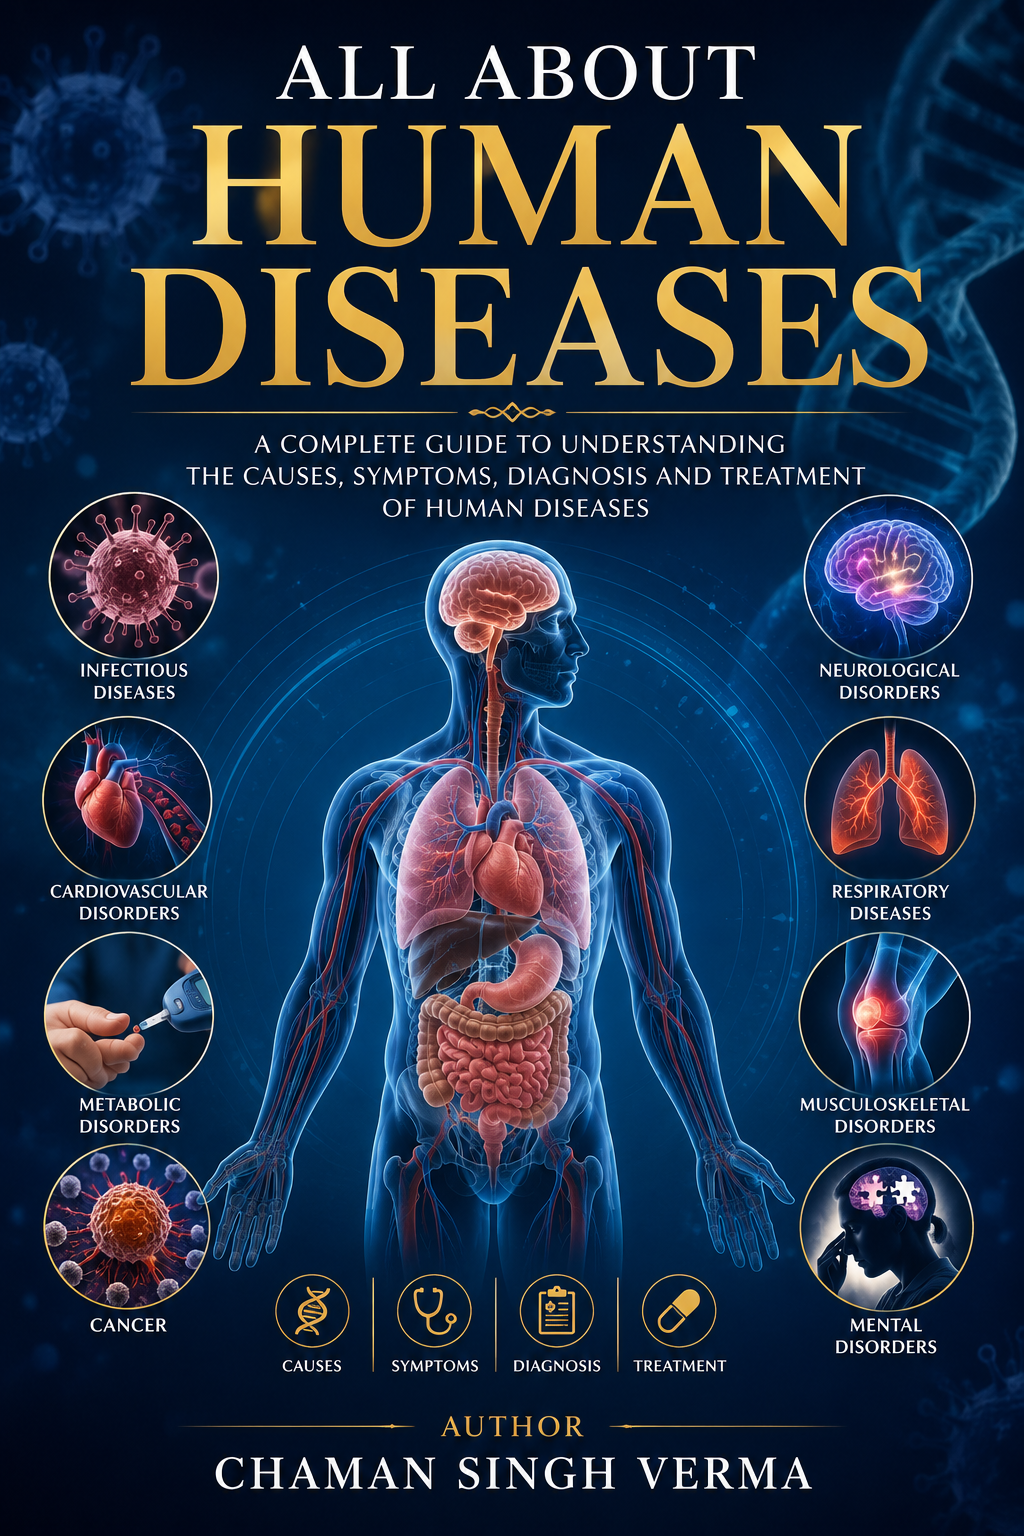
\includepdf[pages=1]{frontpage.png}

\frontmatter

\maketitle
\thispagestyle{empty}

\vfill
\begin{center}
\rule{0.6\textwidth}{0.4pt}\\[12pt]
{\small
This comprehensive report catalogs human diseases organized by the primary
organ or organ system affected. Each chapter provides an overview of the
organ's anatomy and function, followed by detailed entries covering the
most significant diseases---their etiology, pathophysiology, clinical
presentation, diagnosis, and treatment. The report spans all major organ
systems of the human body, from the brain and nervous system to the
reproductive organs, providing a thorough medical reference for students,
educators, and practitioners.}
\\[12pt]
\rule{0.6\textwidth}{0.4pt}
\end{center}
\vfill

\tableofcontents


\mainmatter

% ============================================================
\chapter{Brain and Nervous System Diseases}
\label{ch:brain}
The brain is the command center of the human body, weighing approximately 1.4 kg and containing roughly 86 billion neurons. It controls voluntary and involuntary actions, processes sensory information, governs cognition and emotion, and maintains homeostasis. The brain is protected by the skull, three meningeal layers, and cerebrospinal fluid. Diseases of the brain and nervous system represent some of the most debilitating conditions in medicine, affecting movement, sensation, cognition, and vital functions.

%-------------------------------------------------------------
\section{Brain Tumors}
%-------------------------------------------------------------

%-------------------------------------------------------------

%-------------------------------------------------------------

%-------------------------------------------------------------

Brain tumors represent a heterogeneous group of primary and metastatic central nervous system neoplasms classified by cell of origin, histology, and WHO grade. Primary brain tumors originate within cranial parenchymal cells, meninges, or cranial nerves, whereas metastatic lesions arise from systemic malignancies spreading hematogenously to the neuroaxis. Progressive tumor expansion increases intracranial pressure, producing focal neurological deficits, cognitive decline, and seizures requiring multimodality therapy.

%-------------------------------------------------------------

%-------------------------------------------------------------

%-------------------------------------------------------------

%-------------------------------------------------------------

\label{sec:Brain Tumors}
%-------------------------------------------------------------%-------------------------------------------------------------

\subsection{Glioblastoma}
\index{Glioblastoma}
\label{sec:Glioblastoma}

Glioblastoma is a WHO grade 4 astrocytoma and the most common and aggressive primary malignant brain tumor in adults. The condition results from rapid infiltrative growth with microvascular proliferation and areas of necrosis; the IDH-wildtype molecular profile is characteristic. Clinical features depend on tumor location but typically include progressive headache, seizures, focal neurological deficits, and cognitive changes. Diagnosis is based on MRI showing a ring-enhancing lesion with surrounding edema and mass effect. Management follows the Stupp protocol: maximal safe surgical resection followed by concurrent temozolomide chemotherapy and radiotherapy, then adjuvant temozolomide; MGMT promoter methylation status predicts response to temozolomide; tumor-treating fields (TTFields) have shown incremental survival benefit. Prognosis is poor despite aggressive treatment, with median survival of approximately 15 months.

\subsection{Medulloblastoma}
\index{Medulloblastoma}
\label{sec:Medulloblastoma}
Medulloblastoma is the most common malignant brain tumor of childhood, arising in the cerebellum or posterior fossa, and belongs to the group of embryonal tumors classified into molecular subgroups (WNT, SHH, Group 3, Group 4) with distinct prognoses. The condition results from malignant transformation of primitive neuroectodermal cells. Clinical features include headache, vomiting (especially morning), ataxia, and signs of hydrocephalus from fourth ventricle obstruction. Diagnosis involves MRI showing a posterior fossa mass and cerebrospinal fluid cytology for staging. Management includes maximal surgical resection, craniospinal irradiation, and adjuvant chemotherapy; risk-adapted therapy aims to reduce long-term neurocognitive and endocrine sequelae in survivors. Prognosis varies by molecular subgroup, with the WNT subgroup having the best prognosis.

\subsection{Meningioma}
\index{Meningioma}
\label{sec:Meningioma}
Meningioma is the most common primary intracranial tumor, arising from arachnoid cap cells; it is usually benign (WHO grade 1), slow-growing, and attached to the dura; meningiomas are more common in women and associated with prior radiation, neurofibromatosis type 2, and high progesterone receptor expression. The condition results from neoplastic proliferation of arachnoid cap cells. Most are asymptomatic and discovered incidentally on imaging; symptomatic meningiomas cause headaches, seizures, or focal deficits depending on location. Diagnosis is based on MRI revealing a well-circumscribed, homogeneously enhancing dural-based mass with a dural tail. Management involves observation for small, asymptomatic lesions; surgical resection is the mainstay for symptomatic or growing tumors; atypical (grade 2) and anaplastic (grade 3) meningiomas require adjuvant radiotherapy. Prognosis is excellent for benign meningiomas.

\subsection{Neurofibromatosis Type 1}
\index{Neurofibromatosis Type 1}
\label{sec:Neurofibromatosis Type 1}
Neurofibromatosis type 1 (NF1, von Recklinghausen disease) is an autosomal dominant neurocutaneous disorder caused by mutations in the NF1 gene encoding neurofibromin, a Ras-GTPase tumor suppressor, affecting 1 in 3,000 births. The condition results from loss of neurofibromin function, leading to uncontrolled Ras signaling and increased cell proliferation. Clinical features include caf\'{e}-au-lait spots ($\ge$ 6 spots $>$ 5 mm in children, $>$ 15 mm in adults), axillary and inguinal freckling, Lisch nodules (iris hamartomas), neurofibromas (cutaneous, subcutaneous, plexiform), optic pathway gliomas, osseous dysplasia, and increased risk of malignant peripheral nerve sheath tumors. Diagnosis is based on NIH consensus criteria ($\ge$ 2 of 7 features). Management involves annual ophthalmologic and neurologic monitoring, surgical excision of symptomatic neurofibromas, MEK inhibitor therapy (selumetinib) for symptomatic plexiform neurofibromas, and surveillance for malignancies. Prognosis is variable; life expectancy is reduced by 10--15 years, primarily due to malignancy and cardiovascular disease.

\subsection{Pituitary Adenoma}
\index{Pituitary Adenoma}
\label{sec:Pituitary Adenoma}
Pituitary adenomas are benign neoplasms of the anterior pituitary gland, classified as microadenomas (less than 10 mm) or macroadenomas (10 mm or greater). The condition results from clonal proliferation of pituitary cells. Functioning adenomas secrete excess hormones: prolactinomas (galactorrhea, amenorrhea, hypogonadism), GH-secreting adenomas (acromegaly or gigantism), ACTH-secreting adenomas (Cushing's disease), and TSH-secreting adenomas (central hyperthyroidism); non-functioning adenomas present with mass effects including bitemporal hemianopia from optic chiasm compression, headaches, and hypopituitarism. Clinical features depend on hormone secretion and tumor size. Diagnosis involves hormonal evaluation and MRI of the sella. Management varies: prolactinomas respond to dopamine agonists (cabergoline); other functioning and non-functioning adenomas typically require transsphenoidal surgery, with radiation for residual or recurrent disease. Prognosis is generally favorable.

\subsection{Schwannoma}
\index{Schwannoma}
\label{sec:Schwannoma}
Schwannomas are benign nerve sheath tumors arising from Schwann cells; vestibular schwannomas (acoustic neuromas) are the most common intracranial schwannomas. The condition results from neoplastic proliferation of Schwann cells. Bilateral vestibular schwannomas are pathognomonic of neurofibromatosis type 2. Clinical features of vestibular schwannoma include unilateral sensorineural hearing loss, tinnitus, and imbalance. Diagnosis is based on MRI showing a cerebellopontine angle mass with an ice-cream cone appearance in the internal auditory canal. Management options include observation with serial imaging, stereotactic radiosurgery (Gamma Knife), and microsurgical resection; facial nerve preservation is a key surgical goal. Prognosis is excellent for benign schwannomas.

%-------------------------------------------------------------
\section{Cerebrovascular Diseases}
%-------------------------------------------------------------

%-------------------------------------------------------------

%-------------------------------------------------------------

%-------------------------------------------------------------

%-------------------------------------------------------------

%-------------------------------------------------------------

%-------------------------------------------------------------

%-------------------------------------------------------------

\label{sec:Cerebrovascular Diseases}
%-------------------------------------------------------------%-------------------------------------------------------------

\subsection{Cerebral Aneurysm}
\index{Cerebral Aneurysm}
\label{sec:Cerebral Aneurysm}
A cerebral aneurysm is a focal dilation of a cerebral artery, most commonly at bifurcation sites in the Circle of Willis; saccular (berry) aneurysms are the most prevalent type. The condition results from weakness in the arterial wall. Risk factors include hypertension, smoking, family history, connective tissue disorders (e.g., Ehlers-Danlos syndrome type II, autosomal dominant polycystic kidney disease), and female sex. Most are asymptomatic and discovered incidentally, but rupture causes subarachnoid hemorrhage with high mortality (approximately 40\%). Diagnosis is by CT angiography, MR angiography, or digital subtraction angiography. Management of unruptured aneurysms may involve observation or prophylactic treatment depending on size, location, and patient factors; ruptured aneurysms require urgent surgical clipping or endovascular coiling. Prognosis is good for unruptured aneurysms but poor following rupture.

\subsection{Cerebral Venous Thrombosis}
\index{Cerebral Venous Thrombosis}
\label{sec:Cerebral Venous Thrombosis}
Cerebral venous thrombosis is a thrombosis of the dural venous sinuses or cerebral veins that leads to impaired venous drainage, increased intracranial pressure, and potential venous infarction; it accounts for less than 1\% of all strokes but disproportionately affects young adults and women, particularly those using oral contraceptives or during pregnancy and the puerperium. The condition results from thrombotic occlusion of cerebral veins or dural sinuses. Clinical features vary widely and may include headache, seizures, focal neurological deficits, papilledema, and altered consciousness. Diagnosis requires CT or MR venography showing a filling defect in the venous sinuses. Management consists of anticoagulation (even in the presence of hemorrhagic venous infarction), management of raised intracranial pressure, and treatment of seizures. Prognosis is generally favorable with prompt diagnosis and treatment.

\subsection{Hemorrhagic Stroke}
\index{Hemorrhagic Stroke}
\label{sec:Hemorrhagic Stroke}
Hemorrhagic stroke is a cerebrovascular event resulting from rupture of a blood vessel within the brain, leading to intraparenchymal or subarachnoid hemorrhage. Intracerebral hemorrhage (ICH) is often associated with chronic hypertension, cerebral amyloid angiopathy, vascular malformations, or coagulopathy; subarachnoid hemorrhage (SAH) most commonly results from rupture of a cerebral aneurysm. The condition results from spontaneous rupture of a cerebral blood vessel. Clinical features include sudden severe headache, vomiting, decreased consciousness, and focal neurological deficits that may progress rapidly; SAH presents with thunderclap headache, meningismus, and loss of consciousness. Diagnosis is based on CT head as the initial diagnostic study. Management of ICH focuses on blood pressure control, reversal of anticoagulation, and neurosurgical intervention when indicated; SAH requires urgent neurosurgical clipping or endovascular coiling of the aneurysm with nimodipine to prevent vasospasm. Prognosis depends on hemorrhage location, size, and timeliness of intervention.

\subsection{Ischemic Stroke}
\index{Ischemic Stroke}
\label{sec:Ischemic Stroke}
Ischemic stroke is a focal brain infarction caused by occlusion of a cerebral artery by a thrombus or embolus, accounting for approximately 85\% of all strokes. The condition results from thrombotic or embolic arterial occlusion leading to focal brain ischemia and infarction. Common etiologies include atherosclerotic large-vessel disease, cardioembolism (e.g., atrial fibrillation), small-vessel occlusive disease (lacunar stroke), and cryptogenic causes. Clinical features depend on the vascular territory affected: middle cerebral artery occlusion causes contralateral hemiparesis, hemisensory loss, and aphasia (if dominant hemisphere); posterior circulation strokes produce visual field defects, ataxia, and crossed deficits. Diagnosis involves urgent non-contrast CT to exclude hemorrhage, followed by CT angiography and perfusion imaging. Management includes intravenous thrombolysis with alteplase (within 4.5 hours) and mechanical thrombectomy for large-vessel occlusions (up to 24 hours in selected patients); secondary prevention includes antithrombotic therapy, statins, and risk factor modification. Prognosis depends on infarct size, location, and timeliness of intervention.

\subsection{Transient Ischemic Attack}
\index{Transient Ischemic Attack}
\label{sec:Transient Ischemic Attack}
A transient ischemic attack (TIA) is a temporary episode of neurological dysfunction caused by focal brain, spinal cord, or retinal ischemia without acute infarction; TIAs are critical warning signs, with the risk of subsequent stroke being highest in the first 48 hours (up to 10\%). The condition results from temporary focal ischemia. Clinical features mirror those of ischemic stroke but resolve completely, typically within minutes to hours. Diagnosis involves brain imaging, vascular imaging (carotid ultrasound, CT or MR angiography), cardiac evaluation, and laboratory studies; the ABCD2 score helps stratify short-term stroke risk. Management includes antiplatelet therapy (aspirin, clopidogrel, or combination), statins, antihypertensives, and carotid endarterectomy or stenting for significant ipsilateral carotid stenosis. Prognosis is good with prompt intervention and risk factor modification.

%-------------------------------------------------------------
\section{Demyelinating and White Matter Diseases}
%-------------------------------------------------------------

%-------------------------------------------------------------

%-------------------------------------------------------------

%-------------------------------------------------------------

%-------------------------------------------------------------

%-------------------------------------------------------------

%-------------------------------------------------------------

%-------------------------------------------------------------

\label{sec:Demyelinating and White Matter Diseases}
%-------------------------------------------------------------%-------------------------------------------------------------

\subsection{Central Pontine Myelinolysis}
\index{Central Pontine Myelinolysis}
\label{sec:Central Pontine Myelinolysis}
Central pontine myelinolysis, also known as osmotic demyelination syndrome, is a non-inflammatory demyelinating condition of the pons caused by overly rapid correction of hyponatremia. The condition results from osmotic stress leading to oligodendrocyte damage and demyelination. Clinical features include spastic quadriparesis, pseudobulbar palsy (dysphagia, dysarthria, emotional lability), and in severe cases, locked-in syndrome. Diagnosis is based on MRI showing a characteristic symmetric T2-hyperintense lesion in the central basis pontis. Management is primarily preventive: serum sodium should be corrected at a rate not exceeding 8--10 mmol/L in 24 hours; treatment is supportive once established. Prognosis is variable, with recovery being partial or absent depending on severity.

\subsection{Guillain-Barr\'{e} Syndrome}
\index{Guillain-Barr\'{e} Syndrome}
\label{sec:Guillain-Barré Syndrome}
Guillain-Barr\'{e} syndrome is an acute, immune-mediated polyneuropathy characterized by rapidly progressive, symmetric limb weakness with areflexia; it often follows a respiratory or gastrointestinal infection by 1--4 weeks, with \textit{Campylobacter jejuni}, cytomegalovirus, Epstein-Barr virus, and Zika virus being common triggers. The condition results from an autoimmune attack on peripheral nerves triggered by preceding infection. The most common variant is acute inflammatory demyelinating polyneuropathy (AIDP), while acute motor axonal neuropathy (AMAN) is more prevalent in Asia. Clinical features include rapidly progressive symmetric weakness, areflexia, and possible autonomic dysfunction (tachycardia, blood pressure lability) and respiratory muscle weakness requiring ventilatory support. Diagnosis is based on clinical features and CSF analysis showing albuminocytological dissociation (elevated protein with normal cell count). Management includes intravenous immunoglobulin (IVIg) or plasmapheresis. Prognosis is variable, with most patients recovering; 5--10\% die and 10--20\% have significant residual disability.

%-------------------------------------------------------------
\section{Disorders of Consciousness}
%-------------------------------------------------------------

%-------------------------------------------------------------

%-------------------------------------------------------------

%-------------------------------------------------------------

%-------------------------------------------------------------

%-------------------------------------------------------------

%-------------------------------------------------------------

%-------------------------------------------------------------

\label{sec:Disorders of Consciousness}
%-------------------------------------------------------------%-------------------------------------------------------------

\subsection{Coma}
\index{Coma}
\label{sec:Coma}
Coma is a state of profound unconsciousness in which the patient cannot be aroused and does not respond to external stimuli. The condition results from dysfunction of the ascending reticular activating system in the brainstem or bilateral cerebral hemispheres; common causes include traumatic brain injury, stroke, intracranial hemorrhage, status epilepticus, metabolic encephalopathy, drug intoxication, infections, and hypoxic-ischemic brain injury. Clinical features include unresponsiveness to external stimuli with eyes closed. Diagnosis is based on clinical assessment using the Glasgow Coma Scale (score 3--15), urgent neuroimaging, and laboratory studies. Management targets the underlying cause, with supportive measures including airway management, intracranial pressure monitoring, and prevention of secondary brain injury. Prognosis varies widely depending on the cause and severity of injury.

\subsection{Persistent Vegetative State}
\index{Persistent Vegetative State}
\label{sec:Persistent Vegetative State}
A persistent vegetative state is a condition of wakeful unconsciousness in which the patient has sleep-wake cycles and may open their eyes spontaneously but shows no evidence of awareness of self or environment. The condition results from severe diffuse brain injury, cardiac arrest, or massive stroke. When it persists beyond one month, it is termed persistent; beyond three months for non-traumatic and twelve months for traumatic etiologies, it is termed permanent. Clinical features include spontaneous eye opening with sleep-wake cycles but no purposeful responses. Diagnosis is challenging and may be aided by functional neuroimaging (fMRI) and EEG. Management is supportive; ethical and legal considerations surrounding withdrawal of life-sustaining treatment are complex. Prognosis for recovery of consciousness is poor once permanent criteria are met.

%-------------------------------------------------------------
\section{Epilepsy and Seizure Disorders}
%-------------------------------------------------------------

%-------------------------------------------------------------

%-------------------------------------------------------------

%-------------------------------------------------------------

%-------------------------------------------------------------

%-------------------------------------------------------------

%-------------------------------------------------------------

%-------------------------------------------------------------

\label{sec:Epilepsy and Seizure Disorders}
%-------------------------------------------------------------%-------------------------------------------------------------

\subsection{Epilepsy}
\index{Epilepsy}
\label{sec:Epilepsy}
Epilepsy is a chronic neurological disorder characterized by recurrent, unprovoked seizures resulting from abnormal excessive or synchronous neuronal activity in the brain; it is defined by two or more unprovoked seizures occurring more than 24 hours apart, or one unprovoked seizure with a high recurrence risk. The condition results from genetic, structural (e.g., cortical dysplasia, tumor, stroke), infectious, metabolic, or immune causes. Seizure classification distinguishes focal (partial) from generalized seizures, with further subtypes including absence, tonic-clonic, myoclonic, atonic, and tonic seizures. Clinical features depend on seizure type. Diagnosis relies on clinical history, EEG showing epileptiform discharges, and neuroimaging. Management involves antiseizure medications selected based on seizure type and syndrome classification; drug-resistant epilepsy may be treated with epilepsy surgery, vagus nerve stimulation, or responsive neurostimulation. Prognosis is variable, with many patients achieving seizure control with appropriate therapy.

\subsection{Febrile Seizures}
\index{Febrile Seizures}
\label{sec:Febrile Seizures}
Febrile seizures are the most common seizures in childhood, occurring in 2--5\% of children between 6 months and 5 years of age. The condition results from fever (temperature greater than 38 degrees Celsius) associated with an extracranial infection, in the absence of central nervous system infection or defined electrolyte imbalance. Simple febrile seizures are generalized, last less than 15 minutes, and do not recur within 24 hours; complex febrile seizures are focal, prolonged (greater than 15 minutes), or recurrent. Clinical features include generalized or focal seizure activity triggered by fever. Diagnosis is clinical, after excluding central nervous system infection. Management is supportive; antipyretics prevent recurrence only partially, and prophylactic anticonvulsants are generally not recommended. Prognosis is excellent, with most children outgrowing febrile seizures by age 6.

\subsection{Temporal Lobe Epilepsy}
\index{Temporal Lobe Epilepsy}
\label{sec:Temporal Lobe Epilepsy}
Temporal lobe epilepsy is the most common form of focal epilepsy in adults, often arising from mesial temporal sclerosis (hippocampal sclerosis). The condition results from hippocampal sclerosis, low-grade gliomas, focal cortical dysplasia, or dual pathology. Seizures typically begin with an aura (d\'{e}j\`{a} vu, epigastric rising, fear, olfactory or gustatory hallucinations), followed by impaired awareness, automatisms (lip smacking, hand fumbling), and postictal confusion. Clinical features include focal seizures with impaired awareness. Diagnosis is based on EEG showing temporal interictal epileptiform discharges and MRI revealing hippocampal atrophy and T2/FLAIR signal changes in mesial temporal sclerosis. Management involves antiseizure medications; drug resistance is common, and temporal lobe epilepsy is the most surgically amenable epilepsy, with anterior temporal lobectomy achieving seizure freedom in 60--80\% of selected patients. Prognosis is favorable with surgical treatment for drug-resistant cases.

%-------------------------------------------------------------
\section{Infections of the Brain}
%-------------------------------------------------------------

%-------------------------------------------------------------

%-------------------------------------------------------------

%-------------------------------------------------------------

%-------------------------------------------------------------

%-------------------------------------------------------------

%-------------------------------------------------------------

%-------------------------------------------------------------

\label{sec:Infections of the Brain}
%-------------------------------------------------------------%-------------------------------------------------------------

\subsection{Bacterial Meningitis}
\index{Bacterial Meningitis}
\label{sec:Bacterial Meningitis}
Bacterial meningitis is an acute, life-threatening infection of the leptomeninges and cerebrospinal fluid; the most common causative organisms vary by age: \textit{Streptococcus pneumoniae} and \textit{Neisseria meningitidis} in adults, \textit{Group B Streptococcus} and \textit{Escherichia coli} in neonates, and \textit{Haemophilus influenzae} type b (in unvaccinated populations). The condition results from bacterial invasion of the subarachnoid space. Clinical features include severe headache, high fever, neck stiffness (nuchal rigidity), photophobia, altered mental status, and petechial rash (meningococcal disease); Kernig's and Brudzinski's signs may be positive. Diagnosis requires lumbar puncture showing elevated opening pressure, turbid CSF with neutrophilic pleocytosis, elevated protein, low glucose, and positive Gram stain and culture. Management involves empiric treatment with ceftriaxone plus vancomycin, which should not be delayed; dexamethasone improves outcomes in pneumococcal meningitis. Prognosis depends on the causative organism and timeliness of treatment.

\subsection{Brain Abscess}
\index{Brain Abscess}
\label{sec:Brain Abscess}
A brain abscess is a focal collection of pus within the brain parenchyma, resulting from hematogenous spread, contiguous infection (sinusitis, otitis media, dental infection), or direct inoculation (trauma, neurosurgery); common organisms include \textit{Streptococcus} species, \textit{Staphylococcus aureus}, and anaerobes. The condition results from bacterial infection leading to focal suppuration within brain tissue. Clinical features include headache, fever, focal neurological deficits, seizures, and altered consciousness. Diagnosis is based on MRI with contrast showing a ring-enhancing lesion with surrounding edema and mass effect. Management involves targeted intravenous antibiotics (guided by culture when possible) and, for larger abscesses (greater than 2.5 cm), neurosurgical aspiration or excision. Prognosis has improved significantly with modern imaging and treatment.

\subsection{Neurocysticercosis}
\index{Neurocysticercosis}
\label{sec:Neurocysticercosis}
Neurocysticercosis is the most common parasitic infection of the central nervous system, caused by the larval stage of \textit{Taenia solium} (pork tapeworm); it is endemic in Latin America, Asia, and Africa. The condition results from encystment of larval forms in brain parenchyma, ventricles, or subarachnoid space. Clinical manifestations depend on cyst location and stage and include seizures (the most common presentation worldwide), headache, focal deficits, and hydrocephalus. Diagnosis is supported by neuroimaging showing characteristic cysts (vesicular, colloidal, granular, or calcified stages) and serological testing. Management varies by stage: albendazole and praziquantel for viable cysts with corticosteroid coverage, antiepileptic drugs for seizures, and neurosurgical intervention for hydrocephalus or large symptomatic cysts. Prognosis is generally favorable with appropriate treatment.

\subsection{Viral Encephalitis}
\index{Viral Encephalitis}
\label{sec:Viral Encephalitis}
Viral encephalitis is an inflammation of the brain parenchyma caused by viral infection; herpes simplex virus type 1 (HSV-1) is the most common cause of sporadic fatal encephalitis, typically affecting the temporal and frontal lobes, while other causes include enteroviruses, arboviruses (West Nile, Japanese encephalitis), and varicella-zoster virus. The condition results from direct viral invasion of brain parenchyma. Clinical features include fever, headache, altered consciousness, behavioral changes, seizures, and focal neurological deficits. Diagnosis relies on MRI (temporal lobe involvement in HSV), CSF analysis (lymphocytic pleocytosis, PCR for viral DNA), and EEG. Management involves intravenous acyclovir for HSV encephalitis, which should be initiated empirically. Prognosis is guarded, with significant neurological sequelae in survivors despite treatment.

%-------------------------------------------------------------
\section{Neurodegenerative Diseases}
%-------------------------------------------------------------

%-------------------------------------------------------------

%-------------------------------------------------------------

%-------------------------------------------------------------

%-------------------------------------------------------------

%-------------------------------------------------------------

%-------------------------------------------------------------

%-------------------------------------------------------------

\label{sec:Neurodegenerative Diseases}
%-------------------------------------------------------------%-------------------------------------------------------------

\subsection{Alzheimer's Disease}
\index{Alzheimer's Disease}
\label{sec:Alzheimer's Disease}
Alzheimer's disease is a progressive neurodegenerative disorder and the most common cause of dementia, accounting for 60--70\% of cases. The condition results from the accumulation of amyloid-beta (A$\beta$) plaques between neurons and neurofibrillary tangles composed of hyperphosphorylated tau protein within neurons. Risk factors include advancing age, family history, the apolipoprotein E4 allele, cardiovascular risk factors, and low educational attainment. Clinical features include insidious memory impairment, particularly of recent events, progressing to global cognitive decline, disorientation, language difficulties, and eventual loss of independence. Diagnosis is based on clinical assessment, neuropsychological testing, neuroimaging showing hippocampal atrophy and reduced glucose metabolism on PET, and cerebrospinal fluid biomarkers (A$\beta$42, tau, phospho-tau). Management involves symptomatic treatment with cholinesterase inhibitors (donepezil, rivastigmine, galantamine) and memantine; disease-modifying therapies targeting amyloid remain under investigation. Prognosis is progressive decline with modest benefit from available therapies.

\subsection{Amyotrophic Lateral Sclerosis}
\index{Amyotrophic Lateral Sclerosis}
\label{sec:Amyotrophic Lateral Sclerosis}
Amyotrophic lateral sclerosis is a fatal motor neuron disease characterized by progressive degeneration of both upper and lower motor neurons in the motor cortex, brainstem, and spinal cord. About 10\% of cases are familial, with mutations in SOD1, C9orf72, TARDBP, and FUS genes. The condition results from progressive motor neuron degeneration. Clinical features include focal muscle weakness, atrophy, fasciculations, spasticity, and hyperreflexia; bulbar involvement causes dysarthria and dysphagia. Diagnosis relies on the revised El Escorial criteria, supported by electromyography and exclusion of mimics. Management involves riluzole and edaravone to modestly slow progression, non-invasive ventilation, and multidisciplinary care. Prognosis is poor, with respiratory failure typically causing death within 3--5 years of onset.

\subsection{Dystonia}
\index{Dystonia}
\label{sec:Dystonia}
Dystonia is a movement disorder characterized by sustained or intermittent muscle contractions causing abnormal, often repetitive, movements, postures, or both, with a prevalence of 1 in 3,000. The condition results from dysfunction of the basal ganglia-thalamo-cortical motor circuit, with genetic forms caused by mutations in genes including TOR1A (DYT1, early-onset generalized), THAP1 (DYT6, mixed phenotype), GCH1 (DYT5, dopa-responsive dystonia), and SGCE (DYT11, myoclonus-dystonia). Clinical features vary by distribution: focal (most common, e.g., cervical dystonia/spasmodic torticollis, blepharospasm, oromandibular dystonia, laryngeal dystonia/spasmodic dysphonia, writer's cramp), segmental (involving two contiguous body regions), multifocal, hemidystonia, or generalized. Dystonic movements are typically directional, patterned, and often action-specific, worsened by stress and fatigue, and may be alleviated by sensory tricks (geste antagoniste). Diagnosis is clinical with genetic testing for early-onset or familial cases. Management includes oral medications (trihexyphenidyl, benzodiazepines, baclofen, tetrabenazine), botulinum toxin injections (first-line for focal dystonia), deep brain stimulation of the globus pallidus internus (GPi-DBS, most effective for generalized and cervical dystonia), and levodopa trial for suspected dopa-responsive dystonia. Prognosis: focal dystonia is usually non-progressive after initial spread; generalized dystonia may progress over years but stabilize with treatment.

\subsection{Essential Tremor}
\index{Essential Tremor}
\label{sec:Essential Tremor}
Essential tremor is one of the most common movement disorders, affecting 1\% of the general population and 5\% of individuals over 65 years. The condition results from abnormal oscillatory activity in the cerebello-thalamo-cortical circuit, with genetic heterogeneity (autosomal dominant inheritance in familial cases, ETM1/ETM2 loci). Clinical features include bilateral, symmetric postural and kinetic tremor of the upper limbs (6--12 Hz), which may also involve the head (titubation), voice, chin, or trunk. Tremor is typically absent at rest, worsens with goal-directed movement, and is exacerbated by stress, fatigue, and caffeine. Alcohol consumption temporarily reduces tremor amplitude in 50--70\% of patients. Diagnosis is clinical, based on the Movement Disorder Society consensus criteria and exclusion of other causes (Parkinson disease, dystonic tremor, enhanced physiologic tremor, drug-induced tremor). Management includes first-line treatment with propranolol or primidone, alternative agents (topiramate, gabapentin, benzodiazepines), and for medication-refractory cases, deep brain stimulation of the ventral intermediate nucleus (VIM) of the thalamus or focused ultrasound thalamotomy. Prognosis is benign but slowly progressive; disability from tremor may be significant.

\subsection{Friedreich's Ataxia}
\index{Friedreich's Ataxia}
\label{sec:Friedreich's Ataxia}
Friedreich's ataxia is the most common hereditary ataxia, caused by homozygous GAA trinucleotide repeat expansion in the FXN gene encoding frataxin, with a prevalence of 1 in 50,000. The condition results from frataxin deficiency, leading to mitochondrial iron accumulation, oxidative stress, and impaired energy metabolism, primarily affecting the dorsal root ganglia, posterior columns, corticospinal tracts, and cerebellum. Clinical features include progressive gait and limb ataxia, dysarthria, areflexia, loss of vibratory and proprioceptive sensation, extensor plantar responses, scoliosis, pes cavus, hypertrophic cardiomyopathy, and increased risk of diabetes mellitus. Onset is typically in childhood or adolescence (mean age 10--15 years). Diagnosis is based on clinical criteria and confirmed by FXN genetic testing. Management involves symptomatic treatment: physical therapy for balance and mobility, occupational therapy, speech therapy, and orthopedic management of scoliosis. Cardiac monitoring is essential (echocardiography, ECG). Prognosis is progressive; most patients lose ambulation 10--15 years after symptom onset, with mean survival to age 40--50, primarily due to cardiomyopathy.

\subsection{Frontotemporal Dementia}
\index{Frontotemporal Dementia}
\label{sec:Frontotemporal Dementia}
Frontotemporal dementia encompasses a group of neurodegenerative disorders selectively affecting the frontal and temporal lobes; onset typically occurs between ages 40 and 65, making it a common cause of early-onset dementia. The condition results from accumulation of tau, TDP-43, or FUS proteins. Clinical features include behavioral variant FTD with personality changes, disinhibition, apathy, and executive dysfunction; language variants include semantic dementia (progressive loss of word meaning) and non-fluent or agrammatic primary progressive aphasia. Diagnosis is based on MRI showing disproportionate frontal and temporal lobe atrophy. Management is supportive, focusing on behavioral management, speech therapy, and caregiver support. Prognosis is progressive, with no disease-modifying treatment available.

\subsection{Huntington's Disease}
\index{Huntington's Disease}
\label{sec:Huntington's Disease}
Huntington's disease is an autosomal dominant neurodegenerative disorder caused by a CAG trinucleotide repeat expansion in the huntingtin (HTT) gene on chromosome 4. The condition results from mutant huntingtin protein causing progressive degeneration of neurons, particularly in the caudate nucleus and putamen (striatum). Onset typically occurs between ages 30 and 50, with disease severity correlating inversely with the number of CAG repeats. Clinical features include a triad of motor dysfunction (chorea, dystonia, bradykinesia), cognitive decline (executive dysfunction, dementia), and psychiatric disturbances (depression, irritability, psychosis). Diagnosis is confirmed by genetic testing. Management involves symptomatic treatment with tetrabenazine or deutetrabenazine for chorea, antipsychotics, and antidepressants; genetic counseling is essential. Prognosis is progressive and fatal, with no curative treatment available.

\subsection{Motor Neuron Disease}
\index{Motor Neuron Disease}
\label{sec:Motor Neuron Disease}
Motor neuron disease (MND) is a group of progressive neurodegenerative disorders affecting upper motor neurons (UMNs), lower motor neurons (LMNs), or both, with a lifetime risk of 1 in 300. The spectrum includes amyotrophic lateral sclerosis (ALS, most common, both UMN and LMN), progressive bulbar palsy (PBP, predominantly bulbar onset), progressive muscular atrophy (PMA, predominantly LMN), and primary lateral sclerosis (PLS, predominantly UMN). The condition results from TDP-43 pathology, glutamate excitotoxicity, oxidative stress, mitochondrial dysfunction, and impaired protein degradation, with genetic causes including C9orf72 hexanucleotide repeat expansion, SOD1, TARDBP, FUS, and TBK1 mutations. Clinical features include progressive muscle weakness, wasting, fasciculations, spasticity, hyperreflexia (UMN signs), and bulbar symptoms (dysarthria, dysphagia). ALS presentations include limb-onset (70\%), bulbar-onset (25\%), and respiratory-onset (5\%). Cognitive impairment is present in 30--50\% (frontotemporal dementia in 15\%). Diagnosis is based on revised El Escorial criteria, electromyography showing widespread denervation, and exclusion of mimics. Management involves multidisciplinary care, riluzole (extends survival by 2--3 months), edaravone (slows functional decline in early ALS), noninvasive ventilation for respiratory insufficiency, and symptomatic treatments (sialorrhea, spasticity, pain). Prognosis is uniformly fatal in ALS: median survival 3--5 years from symptom onset, with respiratory failure as the most common cause of death.

\subsection{Multiple Sclerosis}
\index{Multiple Sclerosis}
\label{sec:Multiple Sclerosis}
Multiple sclerosis is a chronic autoimmune demyelinating disease of the central nervous system characterized by inflammatory demyelination and axonal injury occurring at different times and locations; the relapsing-remitting form (RRMS) is most common, while progressive forms (primary progressive, secondary progressive) involve gradual neurological deterioration. The condition results from autoimmune-mediated demyelination. Clinical features include episodic neurological deficits such as optic neuritis, transverse myelitis, brainstem syndromes, and sensory or motor disturbances. Diagnosis is based on MRI revealing periventricular, juxtacortical, infratentorial, and spinal cord T2-hyperintense lesions, often with gadolinium enhancement in active plaques; cerebrospinal fluid may show oligoclonal bands. Management involves disease-modifying therapies including interferons, glatiramer acetate, natalizumab, fingolimod, ocrelizumab, and others; acute relapses are treated with high-dose corticosteroids or plasmapheresis. Prognosis varies widely depending on disease course and treatment response.

\subsection{Parkinson's Disease}
\index{Parkinson's Disease}
\label{sec:Parkinson's Disease}
Parkinson's disease is a chronic, progressive neurodegenerative disorder affecting the dopaminergic neurons of the substantia nigra pars compacta in the midbrain. The condition results from loss of pigmented dopaminergic neurons and the presence of Lewy bodies composed of misfolded alpha-synuclein. Clinical features include cardinal motor manifestations---bradykinesia, resting tremor, rigidity, and postural instability---as well as non-motor symptoms such as anosmia, constipation, REM sleep behavior disorder, depression, and autonomic dysfunction, which often precede motor manifestations by years. Diagnosis is clinical, supported by response to dopaminergic therapy and DaT-SPECT imaging. Management involves dopamine replacement with levodopa/carbidopa, dopamine agonists, MAO-B inhibitors, and COMT inhibitors; advanced disease may be managed with deep brain stimulation of the subthalamic nucleus or globus pallidus interna. Prognosis is progressive, with disease-modifying therapies remaining under investigation.

%-------------------------------------------------------------
\section{Peripheral Nerve Diseases}
%-------------------------------------------------------------

%-------------------------------------------------------------

%-------------------------------------------------------------

%-------------------------------------------------------------

%-------------------------------------------------------------

%-------------------------------------------------------------

%-------------------------------------------------------------

%-------------------------------------------------------------

\label{sec:Peripheral Nerve Diseases}
%-------------------------------------------------------------%-------------------------------------------------------------

\subsection{Bell's Palsy}
\index{Bell's Palsy}
\label{sec:Bell's Palsy}
Bell's palsy is an acute, idiopathic, unilateral facial nerve (cranial nerve VII) paralysis of lower motor neuron type and is the most common cause of acute facial palsy. The condition is thought to result from reactivation of herpes simplex virus type 1. Onset is typically abrupt, with complete facial weakness developing over hours to days. Clinical features include inability to close the affected eye, drooping mouth, hyperacusis, and loss of taste on the anterior two-thirds of the tongue. Diagnosis is clinical, after excluding causes such as Ramsay Hunt syndrome, Lyme disease, and stroke. Management with oral corticosteroids (prednisone) started within 72 hours of onset significantly improves outcomes; eye protection is essential to prevent corneal damage. Prognosis is favorable, with most patients recovering fully within weeks to months.

\subsection{Carpal Tunnel Syndrome}
\index{Carpal Tunnel Syndrome}
\label{sec:Carpal Tunnel Syndrome}
Carpal tunnel syndrome is the most common entrapment neuropathy, caused by compression of the median nerve as it passes through the carpal tunnel in the wrist. Risk factors include repetitive wrist movements, pregnancy, hypothyroidism, diabetes, rheumatoid arthritis, and space-occupying lesions. The condition results from mechanical compression of the median nerve within the carpal tunnel. Clinical features include numbness and tingling in the median nerve distribution (thumb, index, middle, and radial half of the ring finger), nocturnal pain, and weakness of the thenar muscles in advanced cases. Diagnosis is based on clinical examination (Phalen's test, Tinel's sign) and nerve conduction studies confirming delayed median nerve conduction across the wrist. Management begins with wrist splinting (especially at night), ergonomic modifications, and corticosteroid injection; surgical carpal tunnel release is indicated for severe or refractory cases. Prognosis is excellent with appropriate treatment.

\subsection{Charcot-Marie-Tooth Disease}
\index{Charcot-Marie-Tooth Disease}
\label{sec:Charcot-Marie-Tooth Disease}
Charcot-Marie-Tooth disease (CMT) is the most common hereditary peripheral neuropathy, affecting 1 in 2,500 individuals. It comprises a genetically heterogeneous group of disorders classified by nerve conduction velocity and inheritance pattern: CMT1 (demyelinating, NCV <38 m/s, autosomal dominant, most commonly PMP22 duplication), CMT2 (axonal, NCV >38 m/s, autosomal dominant, MFN2 most common), CMTX (X-linked, GJB1 mutations), and CMT4 (autosomal recessive). Clinical features include slowly progressive distal muscle weakness and atrophy (beginning in peroneal muscles, leading to foot drop and steppage gait), pes cavus, hammer toes, distal sensory loss, and diminished or absent deep tendon reflexes. Upper extremity involvement occurs later, producing intrinsic hand muscle weakness and claw hand deformity. Diagnosis is based on clinical examination, nerve conduction studies, and genetic testing (next-generation sequencing panels). Management is supportive: physical and occupational therapy, ankle-foot orthoses for foot drop, surgical correction of foot deformities, and pain management for neuropathic pain. Prognosis is generally good; most patients remain ambulatory with normal life expectancy, though the severity varies widely by subtype.

%-------------------------------------------------------------
\section{Traumatic Brain Injury}
%-------------------------------------------------------------

%-------------------------------------------------------------

%-------------------------------------------------------------

%-------------------------------------------------------------

%-------------------------------------------------------------

%-------------------------------------------------------------

%-------------------------------------------------------------

%-------------------------------------------------------------

\label{sec:Traumatic Brain Injury}
%-------------------------------------------------------------%-------------------------------------------------------------

\subsection{Chronic Traumatic Encephalopathy}
\index{Chronic Traumatic Encephalopathy}
\label{sec:Chronic Traumatic Encephalopathy}
Chronic traumatic encephalopathy is a progressive neurodegenerative disease associated with repetitive head impacts, found predominantly in contact sport athletes, military personnel exposed to blast injuries, and victims of repeated physical abuse. The condition results from accumulation of hyperphosphorylated tau protein in neurons and astrocytes, typically in a perivascular distribution at the depths of cortical sulci. Clinical features include behavioral and mood changes (depression, apathy, irritability, impulsivity), cognitive impairment (progressive dementia), and motor abnormalities (parkinsonism); symptoms typically manifest years to decades after the repetitive head trauma. Diagnosis is currently only confirmed postmortem by neuropathological examination. Management is supportive, as no disease-modifying treatment exists. Prognosis is progressive and incurable; the discovery of chronic traumatic encephalopathy has led to significant changes in sports safety protocols.

\subsection{Concussion}
\index{Concussion}
\label{sec:Concussion}
Concussion is a mild traumatic brain injury caused by a direct blow to the head or a biomechanical force transmitted to the brain, resulting in a transient disturbance of neurological function; it is the most common form of traumatic brain injury. The condition results from a complex neurometabolic cascade involving ionic flux, neurotransmitter release, impaired cerebral blood flow regulation, and axonal injury, without macrostructural damage visible on conventional neuroimaging. Clinical features include headache, dizziness, confusion, amnesia, visual disturbances, sensitivity to light and noise, difficulty concentrating, and emotional lability; loss of consciousness occurs in fewer than 10\% of cases. Diagnosis is clinical; CT head is indicated to exclude intracranial hemorrhage in patients with risk factors (age greater than 65, anticoagulant use, focal neurological signs, persistent vomiting, worsening headache). Management involves physical and cognitive rest for 24--48 hours, followed by a graduated return-to-activity protocol. Prognosis is favorable, although post-concussion syndrome (persistent symptoms beyond 4 weeks) occurs in 10--30\% of patients; second impact syndrome is a rare but potentially fatal complication.

\subsection{Epidural Hematoma}
\index{Epidural Hematoma}
\label{sec:Epidural Hematoma}

An epidural hematoma is a traumatic intracranial hemorrhage accumulating between the inner skull table and the dura mater, most commonly resulting from skull fracture crossing the pterion with laceration of the middle meningeal artery. Clinical features include transient loss of consciousness at injury followed by a lucid interval (lasting hours), after which neurological deterioration ensues with severe headache, contralateral hemiparesis, ipsilateral dilated and unreactive pupil (due to uncal herniation with CN III compression), and Cushing triad (hypertension, bradycardia, irregular respiration). Diagnosis is by non-contrast head CT showing a convex, biconvex (lens-shaped) hyperdense collection that does not cross cranial suture lines. Management requires urgent neurosurgical craniotomy and hematoma evacuation to prevent fatal brain herniation. Prognosis is excellent if evacuated promptly before herniation.

\subsection{Subdural Hematoma}
\index{Subdural Hematoma}
\label{sec:Subdural Hematoma}
A subdural hematoma is a traumatic intracranial bleeding accumulating in the potential space between the dura mater and arachnoid mater, resulting from tearing of bridging veins. Acute subdural hematomas follow high-impact trauma; chronic subdural hematomas occur predominantly in elderly patients and alcoholics, where cerebral atrophy stretches bridging veins, making them susceptible to rupture from minor head trauma. Clinical features include headache, confusion, fluctuating consciousness, and focal neurological deficits, developing over hours in acute cases or weeks/months in chronic cases. Diagnosis is established by non-contrast head CT: acute SDH appears crescent-shaped hyperdense; chronic SDH appears hypodense; SDH crosses suture lines but does not cross dural reflections (falx/tentorium). Management of large or symptomatic hematomas involves surgical evacuation (burr holes or craniotomy); small asymptomatic SDHs are managed conservatively. Prognosis depends on underlying brain injury.

%-------------------------------------------------------------
\section{Vestibular Disorders}
%-------------------------------------------------------------

%-------------------------------------------------------------

%-------------------------------------------------------------

%-------------------------------------------------------------

%-------------------------------------------------------------

%-------------------------------------------------------------

%-------------------------------------------------------------

%-------------------------------------------------------------

\label{sec:Vestibular Disorders}
%-------------------------------------------------------------%-------------------------------------------------------------

\subsection{Vertigo}
\index{Vertigo}
\label{sec:Vertigo}
Vertigo is the sensation of spinning or movement of the self or surroundings when there is no actual movement; it is a symptom, not a disease, and may originate from peripheral (inner ear) or central (brainstem, cerebellar) causes. Peripheral vertigo is more common and results from dysfunction of the vestibular apparatus or nerve; causes include benign paroxysmal positional vertigo, vestibular neuritis, labyrinthitis, and M\'{e}ni\`{e}re's disease. Central vertigo results from brainstem or cerebellar pathology; causes include posterior circulation stroke, vestibular migraine, multiple sclerosis, and cerebellar tumors. Clinical features of peripheral vertigo include severe rotational vertigo with nystagmus (beating away from the affected side), nausea, and vomiting; central vertigo tends to be less severe but may be continuous with diplopia, dysarthria, and limb ataxia. Diagnosis involves detailed history, neurological examination, Dix-Hallpike test for BPPV, and neuroimaging when central causes are suspected. Management depends on the underlying cause: canalith repositioning maneuvers for BPPV, vestibular rehabilitation for vestibular neuritis, and stroke protocols for central vertigo; vestibular suppressants provide symptomatic relief but should be used short-term. Prognosis depends on the underlying cause.


% ============================================================
\chapter{Diseases of the Eyes}
\label{ch:eyes}
The human eye is a complex sensory organ responsible for vision, capable of detecting light across a wide range of intensities and resolving fine detail. Disease of the eye can arise from structural abnormalities, infection, inflammation, degeneration, trauma, or systemic conditions manifesting ocularly. Eye diseases range from common refractive errors to blinding conditions such as glaucoma and age-related macular degeneration.

%-------------------------------------------------------------
\section{Cataract}
%-------------------------------------------------------------

%-------------------------------------------------------------

%-------------------------------------------------------------

%-------------------------------------------------------------

Cataracts are characterized by progressive opacification of the crystalline lens, representing the leading cause of reversible blindness globally. Opacification results from oxidative stress, protein aggregation, metabolic derangements, or mechanical trauma disrupting lens fiber transparency. Surgical phacoemulsification with intraocular lens implantation remains the gold standard treatment with outstanding visual restoration outcomes.

%-------------------------------------------------------------

%-------------------------------------------------------------

%-------------------------------------------------------------

%-------------------------------------------------------------

\label{sec:Cataract}
%-------------------------------------------------------------%-------------------------------------------------------------

\subsection{Age-Related Cataract}
\index{Age-Related Cataract}
\label{sec:Age-Related Cataract}
Age-related cataract is an opacification of the crystalline lens and the leading cause of preventable blindness worldwide, resulting from cumulative oxidative damage to lens proteins. The condition results from aggregation of damaged lens proteins that scatter light. Classification by location includes nuclear (yellowing and hardening of the lens nucleus), cortical (peripheral wedge-shaped opacities), and posterior subcapsular (opacity near the posterior capsule, often associated with steroid use). Clinical features include painless progressive blurring of vision, glare sensitivity, decreased color perception, and dimming of vision. Diagnosis is by slit-lamp examination. Management is surgical: phacoemulsification with implantation of an intraocular lens. Prognosis is excellent, with cataract surgery being one of the most commonly performed and cost-effective surgical procedures globally.

\subsection{Congenital Cataract}
\index{Congenital Cataract}
\label{sec:Congenital Cataract}
Congenital cataract is an opacification of the lens present at or shortly after birth, affecting 1--6 per 10,000 live births. The condition may be idiopathic, hereditary (autosomal dominant most common), or associated with systemic conditions (Down syndrome, congenital rubella, galactosemia, Lowe syndrome, persistent fetal vasculature). The condition results from abnormal lens development or metabolic insult in utero. Clinical features include lens opacity present at birth or in early childhood. Diagnosis is by slit-lamp examination. Management involves urgent surgical removal, ideally within the first few weeks of life for unilateral cases, followed by postoperative visual rehabilitation with patching and corrective lenses. Prognosis depends on timing of intervention and compliance with visual rehabilitation.

%-------------------------------------------------------------
\section{Corneal Diseases}
%-------------------------------------------------------------

%-------------------------------------------------------------

%-------------------------------------------------------------

%-------------------------------------------------------------

Corneal diseases encompass infectious, dystrophic, inflammatory, and degenerative disorders affecting the anterior transparent window of the eye. Pathology compromising corneal avascular clarity or curvature disrupts optical light refraction, causing significant visual impairment and pain. Management ranges from topical antimicrobial and anti-inflammatory therapies to lamellar or penetrating keratoplasty corneal transplantation.

%-------------------------------------------------------------

%-------------------------------------------------------------

%-------------------------------------------------------------

%-------------------------------------------------------------

\label{sec:Corneal Diseases}
%-------------------------------------------------------------%-------------------------------------------------------------

\subsection{Fuchs' Endothelial Dystrophy}
\index{Fuchs' Endothelial Dystrophy}
\label{sec:Fuchs' Endothelial Dystrophy}
Fuchs' endothelial corneal dystrophy is a bilateral, progressive disorder of the corneal endothelium characterized by guttae, endothelial cell loss, and corneal edema; it is autosomal dominant and more common in women. The condition results from progressive endothelial cell dysfunction and loss. Early disease is asymptomatic; as the disease progresses, clinical features include morning blurring that improves through the day, glare, and reduced visual acuity; advanced disease causes persistent corneal edema and bullous keratopathy. Diagnosis is by slit-lamp examination and specular microscopy showing reduced endothelial cell density. Management includes hypertonic saline drops for mild edema and endothelial keratoplasty (DMEK or DSAEK) for advanced disease. Prognosis is excellent with surgical intervention.

\subsection{Keratitis}
\index{Keratitis}
\label{sec:Keratitis}
Keratitis is an inflammation of the cornea that may be infectious or non-infectious. Infectious keratitis can be bacterial, viral (herpes simplex), fungal, or amoebic (\textit{Acanthamoeba}). Bacterial keratitis, the most common type, results from corneal infection, often associated with contact lens use or trauma. Clinical features include pain, redness, tearing, decreased vision, and a corneal infiltrate or ulcer; herpes simplex keratitis may present as epithelial (dendritic ulcer) or stromal disease. Diagnosis involves corneal scraping for Gram stain, culture, and sensitivity. Management requires frequent topical antimicrobial agents appropriate for the suspected organism. Prognosis depends on the causative organism and timeliness of treatment; corneal scarring may require transplantation.

\subsection{Keratoconus}
\index{Keratoconus}
\label{sec:Keratoconus}
Keratoconus is a progressive, non-inflammatory ectatic disorder of the cornea characterized by progressive thinning and steepening, resulting in irregular astigmatism and reduced visual acuity; onset is typically in adolescence or early adulthood. Risk factors include eye rubbing, family history, and associated systemic conditions (Ehlers-Danlos syndrome, Marfan syndrome, Down syndrome). The condition results from structural weakening of the corneal stroma. Clinical features include progressive visual distortion and decreased visual acuity; slit-lamp findings include Munson's sign, Vogt's striae, and corneal iron deposition. Diagnosis is based on corneal topography and tomography. Management progresses from spectacles and rigid gas-permeable contact lenses to corneal crosslinking to halt progression, intrastromal corneal ring segments, and ultimately keratoplasty in advanced cases. Prognosis is variable; corneal crosslinking effectively halts progression.

%-------------------------------------------------------------
\section{Dry Eye Disease}
%-------------------------------------------------------------

%-------------------------------------------------------------

%-------------------------------------------------------------

%-------------------------------------------------------------

%-------------------------------------------------------------

%-------------------------------------------------------------

%-------------------------------------------------------------

%-------------------------------------------------------------

\label{sec:section:Dry Eye Disease}
%-------------------------------------------------------------%-------------------------------------------------------------

\subsection{Dry Eye Disease}
\index{Dry Eye Disease}
\label{sec:Dry Eye Disease}
Dry eye disease is a multifactorial disorder of the ocular surface characterized by loss of homeostasis of the tear film, affecting approximately 5--30\% of the global population, with higher prevalence in the elderly, women, and those in arid or windy environments. The condition results from tear film instability due to aqueous-deficient (reduced lacrimal gland production, as in Sj\"{o}gren's syndrome, aging, or medication side effects) or evaporative causes (meibomian gland dysfunction, lid abnormalities, or environmental factors). Clinical features include dryness, grittiness, burning, foreign body sensation, photophobia, and blurred vision; signs include reduced tear break-up time (less than 10 seconds), Schirmer's test less than 5 mm in 5 minutes, corneal staining, and meibomian gland dropout. Diagnosis is clinical, supported by tear osmolarity testing and inflammatory markers. Management is stepwise: artificial tears, punctal plugs, topical cyclosporine A or lifitegrast, secretagogues, warm compresses and lid hygiene, and environmental modifications. Prognosis is variable, with most patients achieving symptom control with appropriate management.

%-------------------------------------------------------------
\section{Glaucoma}
%-------------------------------------------------------------

%-------------------------------------------------------------

%-------------------------------------------------------------

%-------------------------------------------------------------

Glaucoma is a group of progressive optic neuropathies characterized by characteristic structural changes to the optic nerve head and progressive visual field loss. Elevated intraocular pressure resulting from impaired aqueous humor outflow dynamics represents the primary modifiable risk factor for retinal ganglion cell apoptosis. Early therapeutic lowering of intraocular pressure via topical medications, laser trabeculoplasty, or incisional surgery halts irreversible visual loss.

%-------------------------------------------------------------

%-------------------------------------------------------------

%-------------------------------------------------------------

%-------------------------------------------------------------

\label{sec:Glaucoma}
%-------------------------------------------------------------%-------------------------------------------------------------

\subsection{Glaucoma in Children}
\index{Glaucoma in Children}
\label{sec:Glaucoma in Children}
Primary congenital glaucoma is a condition resulting from developmental abnormality of the trabecular meshwork (goniodysgenesis), causing elevated intraocular pressure from birth or early childhood. The condition results from abnormal development of the aqueous outflow pathways. Clinical features include epiphora, blepharospasm, photophobia, buphthalmos, and corneal edema; juvenile open-angle glaucoma presents in older children and adolescents. Diagnosis is based on examination under anesthesia and tonometry. Management involves early surgical intervention (goniotomy or trabeculotomy); secondary childhood glaucoma may result from aphakia, trauma, uveitis, or steroids. Prognosis depends on early intervention to prevent irreversible optic nerve damage and amblyopia.

\subsection{Primary Angle-Closure Glaucoma}
\index{Primary Angle-Closure Glaucoma}
\label{sec:Primary Angle-Closure Glaucoma}
Primary angle-closure glaucoma is an ophthalmic emergency that occurs when the peripheral iris physically obstructs the trabecular meshwork, blocking aqueous humor drainage and causing a rapid rise in intraocular pressure; it is more common in hyperopic eyes with shallow anterior chambers. The condition results from anatomical predisposition leading to iridotrabecular contact. Clinical features of acute angle closure include severe eye pain, headache, nausea, blurred vision, halos around lights, a mid-dilated fixed pupil, and markedly elevated IOP; chronic angle closure may be asymptomatic until advanced. Diagnosis is based on tonometry and gonioscopy. Management of acute angle closure includes immediate topical and systemic IOP-lowering agents followed by laser peripheral iridotomy; fellow eyes should undergo prophylactic iridotomy. Prognosis is excellent with prompt treatment.

\subsection{Primary Open-Angle Glaucoma}
\index{Primary Open-Angle Glaucoma}
\label{sec:Primary Open-Angle Glaucoma}
Primary open-angle glaucoma is the most common form of glaucoma and a leading cause of irreversible blindness worldwide, characterized by progressive optic nerve damage and visual field loss, typically associated with elevated intraocular pressure. The condition results from increased resistance to aqueous humor outflow through the trabecular meshwork despite an open angle between the iris and cornea. The disease is painless and insidious, often remaining undetected until advanced visual field loss. Clinical features include progressive visual field loss, often beginning peripherally. Diagnosis involves tonometry, gonioscopy, optic disc evaluation (cup-to-disc ratio), automated perimetry, and optical coherence tomography. Management includes topical hypotensive medications (prostaglandin analogs, beta-blockers, alpha-agonists, carbonic anhydrase inhibitors), laser trabeculoplasty, and trabeculectomy or tube shunt surgery for refractory cases. Prognosis is variable, with treatment slowing but not reversing disease progression.

%-------------------------------------------------------------
\section{Inflammatory and Autoimmune Eye Diseases}
%-------------------------------------------------------------

%-------------------------------------------------------------

%-------------------------------------------------------------

%-------------------------------------------------------------

%-------------------------------------------------------------

%-------------------------------------------------------------

%-------------------------------------------------------------

%-------------------------------------------------------------

\label{sec:Inflammatory and Autoimmune Eye Diseases}
%-------------------------------------------------------------%-------------------------------------------------------------

\subsection{Scleritis}
\index{Scleritis}
\label{sec:Scleritis}
Scleritis is a severe inflammation of the sclera that is potentially sight-threatening due to complications such as glaucoma, cataract, and posterior segment inflammation; over 50\% of cases are associated with systemic autoimmune disease, particularly rheumatoid arthritis, granulomatosis with polyangiitis, and relapsing polychondritis. The condition results from immune-mediated inflammation of the sclera. Clinical features include deep, boring eye pain, redness, and decreased vision; anterior scleritis may be diffuse, nodular, or necrotizing; posterior scleritis can mimic orbital tumors. Diagnosis is based on clinical examination and imaging when indicated. Management requires systemic corticosteroids and immunosuppressive agents. Prognosis depends on the severity and underlying systemic disease.

\subsection{Uveitis}
\index{Uveitis}
\label{sec:Uveitis}
Uveitis is an intraocular inflammation involving the uveal tract (iris, ciliary body, choroid), classified by anatomical location as anterior uveitis (iritis or iridocyclitis), intermediate uveitis (pars planitis), posterior uveitis (choroiditis), or panuveitis. The condition results from infectious or autoimmune causes, including HLA-B27-associated conditions (ankylosing spondylitis, reactive arthritis), Beh\c{c}et's disease, sarcoidosis, and infections (herpes, syphilis, tuberculosis). Clinical features of anterior uveitis include eye pain, redness, photophobia, and hypopyon; intermediate uveitis features vitreous cells and floaters; posterior uveitis presents with floaters, visual field defects, or decreased vision. Diagnosis is based on slit-lamp and dilated fundus examination. Management uses topical, periocular, or systemic corticosteroids and steroid-sparing immunosuppressive agents for chronic disease; biologics (anti-TNF agents) are used for refractory cases. Prognosis depends on the underlying cause and severity.

%-------------------------------------------------------------
\section{Ocular Surface Disorders}
%-------------------------------------------------------------

%-------------------------------------------------------------

%-------------------------------------------------------------

%-------------------------------------------------------------

%-------------------------------------------------------------

%-------------------------------------------------------------

%-------------------------------------------------------------

%-------------------------------------------------------------

\label{sec:Ocular Surface Disorders}
%-------------------------------------------------------------%-------------------------------------------------------------

\subsection{Conjunctivitis}
\index{Conjunctivitis}
\label{sec:Conjunctivitis}
Conjunctivitis is an inflammation of the conjunctiva and the most common eye disease worldwide, classified as infectious (viral, bacterial), allergic, or chemical or irritant. Viral conjunctivitis, most commonly caused by adenovirus, results from viral infection of the conjunctiva. Bacterial conjunctivitis results from bacterial infection (S. aureus, S. pneumoniae, H. influenzae, N. gonorrhoeae, C. trachomatis). Clinical features of viral conjunctivitis include acute onset, watery discharge, and preauricular lymphadenopathy; bacterial conjunctivitis presents with purulent discharge and eyelids matted shut; allergic conjunctivitis features bilateral itching, tearing, and stringy mucus. Diagnosis is clinical, with Gram stain and culture used for hyperacute or bacterial cases. Management is etiologic: supportive for viral, topical antibiotics for bacterial, and topical antihistamine or mast cell stabilizers for allergic; gonococcal conjunctivitis requires intramuscular ceftriaxone. Prognosis is excellent with appropriate treatment; untreated gonococcal conjunctivitis can lead to corneal perforation within 24 hours.

%-------------------------------------------------------------
\section{Refractive Errors}
%-------------------------------------------------------------

%-------------------------------------------------------------

%-------------------------------------------------------------

%-------------------------------------------------------------

Refractive errors occur when the optical power of the cornea and crystalline lens fails to focus incoming parallel light rays precisely onto the retina. Mismatches between focal length and axial length produce blurred vision at near or distant ranges. Optical correction via spectacles, contact lenses, or keratorefractive laser procedures restores clear visual acuity.

%-------------------------------------------------------------

%-------------------------------------------------------------

%-------------------------------------------------------------

%-------------------------------------------------------------

\label{sec:Refractive Errors}
%-------------------------------------------------------------%-------------------------------------------------------------

\subsection{Astigmatism}
\index{Astigmatism}
\label{sec:Astigmatism}
Astigmatism is a refractive error caused by irregular curvature of the cornea or lens, resulting in different refractive powers in different meridians. The condition results from irregular corneal or lenticular curvature. Clinical features include blurred or distorted vision at both near and distance. Most astigmatism is corneal and regular. Diagnosis is based on refraction testing. Management involves correction with cylindrical lenses (glasses or contact lenses) or refractive surgery; irregular astigmatism may require rigid gas-permeable contact lenses or scleral lenses. Prognosis is excellent with appropriate correction.

\subsection{Hyperopia}
\index{Hyperopia}
\label{sec:Hyperopia}
Hyperopia is a refractive error that occurs when the axial length of the eye is too short or the refractive power is insufficient, causing light to focus behind the retina. The condition results from insufficient refractive power relative to axial length. Mild hyperopia may be accommodated for, especially in young patients. Clinical features include blurred near vision, eye strain, headaches, and in children, esotropia and amblyopia. Diagnosis is based on refraction testing. Management involves correction with convex (plus) lenses; severe hyperopia in childhood requires early correction to prevent amblyopia and strabismus. Prognosis is excellent with correction.

\subsection{Myopia}
\index{Myopia}
\label{sec:Myopia}
Myopia is the most common refractive error worldwide, affecting approximately 30\% of the global population and approaching 80--90\% in some East Asian countries. The condition results from an axial length of the eye that is too long relative to the refractive power of the cornea and lens, causing light to focus in front of the retina. High myopia (sphere $-6.00$ diopters or greater) increases the risk of retinal detachment, choroidal neovascularization, glaucoma, and cataract. Clinical features include blurred distance vision with preserved near vision. Diagnosis is based on refraction testing. Management involves correction with concave (minus) lenses, contact lenses, or refractive surgery (LASIK, PRK, ICL); atropine eye drops and orthokeratology lenses slow myopia progression in children. Prognosis is excellent with correction.

\subsection{Presbyopia}
\index{Presbyopia}
\label{sec:Presbyopia}
Presbyopia is the age-related loss of accommodation, resulting from hardening of the crystalline lens and decreased ciliary muscle function; it is universal, typically becoming symptomatic after age 40. The condition results from age-related changes in the lens and ciliary muscle. Clinical features include difficulty reading small print, especially in dim light, and the need to hold reading material farther away. Diagnosis is based on clinical history and refraction testing. Management includes reading glasses, bifocal or progressive lenses, monovision contact lens arrangements, and multifocal intraocular lenses; surgical options include corneal inlays, scleral implants, and laser procedures. Prognosis is excellent with appropriate correction.

%-------------------------------------------------------------
\section{Retinal Diseases}
%-------------------------------------------------------------

%-------------------------------------------------------------

%-------------------------------------------------------------

%-------------------------------------------------------------

Retinal diseases involve pathologic processes affecting the neurosensory retina, retinal pigment epithelium, and retinal vascular architecture. Damage to these essential structures disrupts phototransduction pathways, leading to severe vision loss or permanent scotomas. Therapies include intravitreal anti-VEGF microinjections, retinal photocoagulation laser treatment, and vitreoretinal surgical reconstruction.

%-------------------------------------------------------------

%-------------------------------------------------------------

%-------------------------------------------------------------

%-------------------------------------------------------------

\label{sec:Retinal Diseases}
%-------------------------------------------------------------%-------------------------------------------------------------

\subsection{Age-Related Macular Degeneration}
\index{Age-Related Macular Degeneration}
\label{sec:Age-Related Macular Degeneration}
Age-related macular degeneration is the leading cause of irreversible central vision loss in individuals over 50 in developed countries, affecting the macula. The condition results from age-related degenerative changes in the retinal pigment epithelium and photoreceptors; risk factors include age, smoking, family history, and genetic variants (complement factor H). Early AMD is characterized by drusen and pigmentary changes; advanced AMD manifests as either dry (atrophic) AMD with geographic atrophy or wet (neovascular) AMD with choroidal neovascularization. Clinical features include progressive central vision loss and distortion. Diagnosis is based on fundus examination and optical coherence tomography. Management of wet AMD involves anti-VEGF intravitreal injections (ranibizumab, aflibercept, bevacizumab); complement inhibitors are under investigation for dry AMD. Prognosis has improved significantly with anti-VEGF therapy for wet AMD.

\subsection{Diabetic Retinopathy}
\index{Diabetic Retinopathy}
\label{sec:Diabetic Retinopathy}
Diabetic retinopathy is a microvascular complication of diabetes mellitus and a leading cause of blindness in working-age adults. The condition results from chronic hyperglycemia damaging retinal capillaries, causing vascular occlusion, non-perfusion, microaneurysms, hemorrhages, hard exudates, and cotton-wool spots (non-proliferative DR). Progression to proliferative DR involves neovascularization driven by retinal ischemia and VEGF upregulation, with risks of vitreous hemorrhage and tractional retinal detachment; diabetic macular edema can occur at any stage. Clinical features include vision loss, which may be asymptomatic until advanced. Diagnosis involves dilated fundus examination and fundus photography. Management includes optimal glycemic control, anti-VEGF intravitreal injections for diabetic macular edema, focal or grid laser photocoagulation, and panretinal photocoagulation for proliferative disease; regular screening is recommended for all diabetic patients. Prognosis depends on glycemic control and stage at diagnosis.

\subsection{Retinal Detachment}
\index{Retinal Detachment}
\label{sec:Retinal Detachment}
Retinal detachment is a separation of the neurosensory retina from the underlying retinal pigment epithelium, constituting an ophthalmic emergency; rhegmatogenous retinal detachment, the most common type, results from a retinal break allowing vitreous fluid to enter the subretinal space. Risk factors include high myopia, prior cataract surgery, trauma, and lattice degeneration. Tractional retinal detachment occurs in proliferative diabetic retinopathy; exudative retinal detachment results from fluid accumulation without a break. Clinical features include sudden onset of floaters, flashing lights, and a curtain-like visual field defect. Diagnosis is based on dilated fundus examination. Management of rhegmatogenous retinal detachment requires surgical repair with pneumatic retinopexy, scleral buckling, or vitrectomy. Prognosis depends on the type, location, and timeliness of repair.

\subsection{Retinitis Pigmentosa}
\index{Retinitis Pigmentosa}
\label{sec:Retinitis Pigmentosa}
Retinitis pigmentosa is a group of inherited retinal dystrophies characterized by progressive degeneration of photoreceptors, primarily rod cells; most cases are inherited (autosomal dominant, autosomal recessive, or X-linked), with over 80 genes identified. The condition results from genetic mutations causing photoreceptor degeneration. Clinical features include night blindness and progressive peripheral visual field constriction (tunnel vision), eventually affecting central vision; fundoscopy reveals bone-spicule pigmentation, waxy pallor of the optic disc, and attenuated retinal vessels. Diagnosis is based on fundus examination and electroretinography showing diminished or absent responses. Management is supportive; vitamin A supplementation may slow progression in some forms; retinal prostheses and gene therapy (voretigene neparvovec for RPE65-mutated RP) offer emerging therapeutic avenues. Prognosis is progressive with no cure currently available.

\subsection{Retinopathy of Prematurity}
\index{Retinopathy of Prematurity}
\label{sec:Retinopathy of Prematurity}
Retinopathy of prematurity is a vasoproliferative retinal disease affecting premature infants, particularly those born before 32 weeks gestation with low birth weight. The condition results from abnormal vascularization of the developing retina, which can lead to tractional retinal detachment and blindness. The disease is classified by zone, stage, and extent of vascular involvement, with plus disease indicating vascular activity. Clinical features depend on disease severity; most mild ROP regresses spontaneously. Diagnosis is based on screening examinations in at-risk premature infants. Management of severe ROP involves anti-VEGF intravitreal injections or laser photocoagulation of the avascular retina. Prognosis is good with timely screening and treatment; long-term follow-up is necessary due to risks of late sequelae including myopia, strabismus, and retinal detachment.

%-------------------------------------------------------------
\section{Strabismus and Amblyopia}
%-------------------------------------------------------------

%-------------------------------------------------------------

%-------------------------------------------------------------

%-------------------------------------------------------------

%-------------------------------------------------------------

%-------------------------------------------------------------

%-------------------------------------------------------------

%-------------------------------------------------------------

\label{sec:Strabismus and Amblyopia}
%-------------------------------------------------------------%-------------------------------------------------------------

\subsection{Amblyopia}
\index{Amblyopia}
\label{sec:Amblyopia}
Amblyopia is reduced best-corrected visual acuity in one or both eyes resulting from abnormal visual development during the critical period of visual maturation (birth to approximately 8 years); it is the most common cause of monocular vision loss in children. The condition results from strabismus, anisometropia, form deprivation (congenital cataract, ptosis), or bilateral high refractive error, leading to failure of normal neural pathway development in the amblyopic eye. Clinical features include reduced visual acuity that cannot be corrected with lenses. Diagnosis is based on visual acuity testing. Management includes corrective lenses, patching or penalization (atropine drops) of the dominant eye, and treatment of the underlying cause. Prognosis is excellent with early intervention.

\subsection{Strabismus}
\index{Strabismus}
\label{sec:Strabismus}
Strabismus is a misalignment of the visual axes of the two eyes that may be horizontal (esotropia, exotropia) or vertical (hypertropia, hypotropia), and may be constant or intermittent, comitant or non-comitant. The condition results from neuromuscular imbalance of the extraocular muscles; onset in childhood may be accommodative, paralytic, or idiopathic; in adults, acquired strabismus may result from cranial nerve palsies (III, IV, VI), thyroid eye disease, myasthenia gravis, or orbital pathology. Clinical features include visible eye misalignment, which can cause amblyopia in children and diplopia in adults. Diagnosis is based on cover testing and ocular motility examination. Management includes corrective lenses, prisms, occlusion therapy, botulinum toxin injection, and surgical realignment of the extraocular muscles. Prognosis is generally good with appropriate treatment.


% ============================================================
\chapter{Diseases of the Ears}
\label{ch:ears}
The ear is the sensory organ responsible for hearing and balance. It is divided into the outer ear (pinna and external auditory canal), middle ear (tympanic membrane, ossicles, and Eustachian tube), and inner ear (cochlea and vestibular apparatus). Diseases of the ear range from common infections to complex disorders of hearing and equilibrium.

%-------------------------------------------------------------
\section{Inner Ear Diseases}
%-------------------------------------------------------------

%-------------------------------------------------------------

%-------------------------------------------------------------

Inner ear diseases involve pathology of the cochlear and vestibular apparatus located within the bony labyrinth of the temporal bone. Disorders of these intricate structures disrupt auditory transduction and spatial orientation mechanisms, leading to sensorineural hearing loss, vertigo, and dysequilibrium. Etiologies include endolymphatic hydrops, autoimmune inflammatory processes, viral infections, vascular compromise, and ototoxic injury.

%-------------------------------------------------------------

%-------------------------------------------------------------

%-------------------------------------------------------------

%-------------------------------------------------------------

\label{sec:Inner Ear Diseases}
%-------------------------------------------------------------%-------------------------------------------------------------

\subsection{Acoustic Neuroma (Vestibular Schwannoma)}
\label{sec:Acoustic Neuroma (Vestibular Schwannoma)}
Vestibular schwannoma is a benign tumor arising from the Schwann cells of the vestibular portion of cranial nerve VIII and is the most common tumor of the cerebellopontine angle. The condition results from neoplastic proliferation of Schwann cells. Bilateral tumors are pathognomonic of neurofibromatosis type 2. Clinical features include unilateral sensorineural hearing loss, tinnitus, and imbalance; larger tumors may compress adjacent structures causing facial numbness (CN V), facial weakness (CN VII), and brainstem compression. Diagnosis is based on MRI with gadolinium, which is the gold standard. Management options include observation with serial imaging (for small, slow-growing tumors), stereotactic radiosurgery, and microsurgical resection. Prognosis is favorable for small tumors, with hearing preservation as a key goal.

\subsection{Benign Paroxysmal Positional Vertigo}
\label{sec:Benign Paroxysmal Positional Vertigo}
Benign paroxysmal positional vertigo is the most common cause of peripheral vertigo, resulting from displaced otoliths from the utricle into the semicircular canals, most commonly the posterior canal. The condition results from movement of calcium carbonate crystals within the semicircular canals. Clinical features include brief episodes (less than 1 minute) of severe vertigo triggered by head movement, with characteristic nystagmus. Diagnosis is based on the Dix-Hallpike test, which reproduces vertigo and reveals torsional-upbeating nystagmus. Management involves canalith repositioning maneuvers (Epley maneuver for posterior canal BPPV), which are highly effective. Prognosis is excellent, although recurrence occurs in 20--50\% of cases.

\subsection{Labyrinthitis}
\label{sec:Labyrinthitis}
Labyrinthitis is an inflammation of the membranous labyrinth of the inner ear that causes both vestibular and auditory dysfunction. The condition results from viral infection, often following an upper respiratory infection; bacterial labyrinthitis is more severe and can result from otogenic or meningogenic spread. Clinical features include vertigo, nausea, vomiting, hearing loss, and tinnitus. Diagnosis is clinical, supported by audiometry and vestibular testing. Management of viral labyrinthitis involves supportive care (vestibular suppressants, antiemetics, followed by vestibular rehabilitation); bacterial labyrinthitis requires aggressive antibiotic therapy and may require labyrinthectomy. Prognosis is favorable for viral labyrinthitis; bacterial labyrinthitis carries a risk of profound hearing loss.

\subsection{Ménière's Disease}
\label{sec:Ménière's Disease}
Ménière's disease is a chronic inner ear disorder characterized by episodic vertigo, fluctuating sensorineural hearing loss (typically low-frequency), tinnitus, and aural fullness. The condition results from endolymphatic hydrops, although the exact pathogenesis remains debated. Onset is typically unilateral, with progression to bilateral disease in 10--30\% of cases over decades. Clinical features include vertigo episodes lasting minutes to hours that may be incapacitating, associated with nausea and vomiting, along with fluctuating hearing loss, tinnitus, and aural fullness. Diagnosis is clinical, supported by audiometry, vestibular testing, and MRI to exclude other causes. Management includes dietary modification (low sodium, caffeine restriction), betahistine, diuretics, intratympanic gentamicin or corticosteroid for refractory cases, and labyrinthectomy or vestibular nerve section as a last resort. Prognosis is variable, with most patients achieving symptom control with treatment.

\subsection{Sudden Sensorineural Hearing Loss}
\label{sec:Sudden Sensorineural Hearing Loss}
Sudden sensorineural hearing loss is an otologic emergency defined as a loss of at least 30 dB over three contiguous audiometric frequencies within 72 hours. The condition results from idiopathic causes, although viral cochleitis, vascular occlusion, autoimmune inner ear disease, or perilymphatic fistula may be implicated. Clinical features include abrupt unilateral hearing loss, often accompanied by tinnitus, vertigo, and aural fullness. Diagnosis is based on audiometry. Management involves high-dose oral or intratympanic corticosteroids, with prompt treatment within 2 weeks being crucial; hyperbaric oxygen therapy may provide additional benefit. Prognosis is variable, with some cases recovering spontaneously and others sustaining permanent hearing loss.

\subsection{Vestibular Neuritis}
\label{sec:Vestibular Neuritis}
Vestibular neuritis is an acute, isolated episode of severe vertigo caused by inflammation of the vestibular nerve without hearing loss. The condition is thought to be viral in etiology, possibly reactivation of herpes simplex virus. Clinical features include sudden-onset, continuous vertigo lasting days to weeks with severe imbalance and nystagmus beating away from the affected side. Diagnosis is based on clinical examination with the head impulse test showing reduced vestibulo-ocular reflex on the affected side. Management involves short-term vestibular suppressants (benzodiazepines, antihistamines) followed by early vestibular rehabilitation. Prognosis is favorable, with most patients recovering fully over weeks.

%-------------------------------------------------------------
\section{Middle Ear Diseases}
%-------------------------------------------------------------

%-------------------------------------------------------------

%-------------------------------------------------------------

%-------------------------------------------------------------

%-------------------------------------------------------------

%-------------------------------------------------------------

%-------------------------------------------------------------

\label{sec:Middle Ear Diseases}
%-------------------------------------------------------------%-------------------------------------------------------------

\subsection{Acute Otitis Media}
\label{sec:Acute Otitis Media}
Acute otitis media is a bacterial or viral infection of the middle ear that affects 80\% of children by age 3. The condition results from Eustachian tube dysfunction secondary to upper respiratory infection, allowing bacterial or viral entry; the most common pathogens are \textit{Streptococcus pneumoniae}, \textit{Haemophilus influenzae}, and \textit{Moraxella catarrhalis}. Clinical features include ear pain, fever, irritability, and hearing loss; otoscopic examination reveals a bulging, erythematous tympanic membrane with loss of landmarks and possible purulent effusion. Diagnosis is based on clinical and otoscopic examination. Management includes analgesics and observation in mild cases, with amoxicillin as first-line antibiotic therapy for moderate-to-severe disease or treatment failure; recurrent acute otitis media may warrant myringotomy with tympanostomy tube placement. Prognosis is excellent with appropriate treatment.

\subsection{Chronic Otitis Media}
\label{sec:Chronic Otitis Media}
Chronic otitis media is a chronic or recurrent perforation of the tympanic membrane with or without active middle ear infection. The condition results from persistent mucosal inflammation or squamous disease (cholesteatoma), which is an abnormal accumulation of keratinizing squamous epithelium that can erode the ossicles, facial nerve, and bony labyrinth. Clinical features include persistent or recurrent otorrhea through a perforated tympanic membrane, hearing loss, and occasional vertigo; cholesteatoma may cause conductive hearing loss, facial nerve palsy, and intracranial complications. Diagnosis is based on otoscopic examination and temporal bone CT. Management is primarily surgical (tympanoplasty, mastoidectomy). Prognosis depends on the extent of disease and success of surgical intervention.

\subsection{Otosclerosis}
\label{sec:Otosclerosis}
Otosclerosis is a primary bone remodeling disorder of the otic capsule that causes progressive conductive hearing loss, typically bilateral, beginning in the third to fourth decade of life, with a female predominance and genetic component (autosomal dominant with variable penetrance). The condition results from abnormal spongy bone formation (active otosclerosis) that replaces normal endochondral bone, most commonly fixing the footplate of the stapes in the oval window. Clinical features include progressive conductive hearing loss. Diagnosis is suggested by a positive Schwartze sign (red hue of the promontory on otoscopy) and confirmed by audiometry showing conductive or mixed hearing loss. Management involves stapedectomy or stapedotomy with prosthetic stapes replacement, which is highly effective; sodium fluoride may slow disease progression. Prognosis is excellent with surgical intervention.

\subsection{Tympanic Membrane Perforation}
\label{sec:Tympanic Membrane Perforation}
Tympanic membrane perforation is a tear in the eardrum that may result from acute otitis media, trauma (penetrating injury, barotrauma, blast injury), or prior tympanostomy tubes. The condition results from mechanical or infectious disruption of the tympanic membrane. Clinical features include hearing loss, brief otalgia, tinnitus, and otorrhea. Diagnosis is based on otoscopic examination. Management involves observation for small perforations, which often heal spontaneously; larger or persistent perforations may require surgical repair (myringoplasty or tympanoplasty). Prognosis is good, with healing enhanced by keeping the ear dry and avoiding nose blowing.

%-------------------------------------------------------------
\section{Outer Ear Diseases}
%-------------------------------------------------------------

%-------------------------------------------------------------

%-------------------------------------------------------------

Outer ear diseases encompass pathology affecting the pinna (auricle) and the external auditory canal extending to the tympanic membrane. These conditions frequently result from mechanical trauma, environmental exposure, infectious pathogens, or dermatological hypersensitivity reactions. Inflammatory and obstructive disorders of the external canal impair sound wave transmission and cause localized pain, otorrhea, and conductive hearing loss.

%-------------------------------------------------------------

%-------------------------------------------------------------

%-------------------------------------------------------------

%-------------------------------------------------------------

\label{sec:Outer Ear Diseases}
%-------------------------------------------------------------%-------------------------------------------------------------

\subsection{Cerumen Impaction}
\label{sec:Cerumen Impaction}
Cerumen impaction is an accumulation of earwax that causes symptoms or obscures the tympanic membrane, affecting approximately 6\% of the general population and up to 30\% of the elderly. The condition results from overproduction of cerumen or from use of cotton swabs and hearing aids that push cerumen deeper into the canal. Clinical features include hearing loss, aural fullness, tinnitus, and otalgia. Diagnosis is based on otoscopic examination. Management involves manual extraction with a curette, irrigation with warm water, or cerumenolytic agents (dilute hydrogen peroxide, mineral oil, glycerin). Prognosis is excellent with proper removal; avoidance of cotton swabs is recommended for prevention.

\subsection{Chondrodermatitis Nodularis Helicis}
\label{sec:Chondrodermatitis Nodularis Helicis}
Chondrodermatitis nodularis helicis is a painful, inflammatory condition affecting the cartilage of the pinna, most commonly the helix or antihelix. The condition results from necrotizing chondritis with overlying epidermal changes, often triggered by chronic pressure during sleep. Clinical features include a small, exquisitely tender nodule with overlying crusting or ulceration, frequently on the side most affected by sleeping pressure. Diagnosis is based on clinical examination and histopathology. Management includes pressure relief (using a donut-shaped pillow), topical corticosteroids, and intralesional corticosteroid injection; refractory cases may require surgical excision. Prognosis is generally good with appropriate treatment.

\subsection{Otitis Externa}
\label{sec:Otitis Externa}
Otitis externa is an infection of the external auditory canal that commonly affects swimmers and individuals with predisposing factors such as water exposure, cotton-swab use, hearing aids, and humid climates. The condition results from inflammation and infection of the canal skin, most commonly caused by \textit{Pseudomonas aeruginosa} and \textit{Staphylococcus aureus}. Clinical features include ear pain (otalgia), pruritus, otorrhea, and a sensation of ear fullness; examination reveals erythema, edema, and tenderness of the canal wall with purulent debris. In severe cases, infection may spread to the surrounding skin (malignant otitis externa), particularly in diabetics and immunocompromised patients. Diagnosis is based on clinical examination. Management involves thorough canal debridement and topical antimicrobial drops (fluoroquinolones or aminoglycosides with corticosteroids); oral antibiotics are reserved for extensive or invasive disease. Prognosis is excellent with appropriate treatment.

%-------------------------------------------------------------
\section{Tinnitus}
%-------------------------------------------------------------

%-------------------------------------------------------------

%-------------------------------------------------------------

%-------------------------------------------------------------

%-------------------------------------------------------------

%-------------------------------------------------------------

%-------------------------------------------------------------

\label{sec:section:Tinnitus}
Tinnitus is the perception of sound in the absence of an external auditory stimulus, affecting millions of individuals worldwide. It is classified as subjective (audible only to the patient, resulting from aberrant neural activity) or objective (audible to an observer, caused by vascular or muscular turbulence). Management focuses on identifying underlying neuro-otological etiologies, sound therapy, cognitive behavioral interventions, and neurostimulation.

%-------------------------------------------------------------%-------------------------------------------------------------

\subsection{Tinnitus}
\label{sec:Tinnitus}
Tinnitus is the perception of sound in the absence of an external auditory stimulus, affecting approximately 10--15\% of adults, with higher prevalence in the elderly. The condition results from maladaptive neural plasticity in the central auditory pathways following peripheral auditory deafferentation; causes include noise-induced hearing loss (the most common cause), age-related hearing loss, ototoxic medications, M\'{e}ni\`{e}re's disease, vestibular schwannoma, otosclerosis, impacted cerumen, and temporomandibular joint disorders. Clinical features include ringing, buzzing, hissing, roaring, or clicking in one or both ears; tinnitus may be associated with depression, anxiety, and insomnia. Diagnosis is based on thorough history, otoscopic examination, and audiometry to assess for hearing loss; MRI with gadolinium is indicated for asymmetric tinnitus or focal neurological findings. Management includes patient education and reassurance, treatment of reversible causes, hearing aids for those with hearing loss, cognitive-behavioral therapy, sound therapy, and tinnitus retraining therapy. Prognosis is variable, with many patients achieving habituation through appropriate management.


% ============================================================
\chapter{Diseases of the Nose and Sinuses}
\label{ch:nose}
The nose serves as the primary airway for respiration, the organ of olfaction, and a conditioning system that warms, humidifies, and filters inspired air. The paranasal sinuses---maxillary, ethmoid, frontal, and sphenoid---are air-filled cavities lined by respiratory mucosa that drain into the nasal cavity. Diseases of the nose and sinuses are extremely prevalent and include allergic, infectious, inflammatory, structural, and neoplastic conditions.

%-------------------------------------------------------------
\section{Allergic and Inflammatory Conditions}
%-------------------------------------------------------------

%-------------------------------------------------------------

%-------------------------------------------------------------

%-------------------------------------------------------------

%-------------------------------------------------------------

%-------------------------------------------------------------

\label{sec:Allergic and Inflammatory Conditions}
%-------------------------------------------------------------%-------------------------------------------------------------

\subsection{Allergic Rhinitis}
\label{sec:Allergic Rhinitis}
Allergic rhinitis is an IgE-mediated inflammatory condition of the nasal mucosa that affects 10--30\% of the global population. The condition results from exposure to airborne allergens (pollens, dust mites, animal dander, molds) triggering IgE-mediated mast cell degranulation. Seasonal allergic rhinitis (hay fever) correlates with pollen seasons, while perennial allergic rhinitis is year-round. Clinical features include sneezing, nasal congestion, rhinorrhea (clear, watery discharge), nasal pruritus, and nasal obstruction; ocular symptoms (itching, tearing, conjunctival injection) are common. Diagnosis is clinical, supported by skin prick testing or specific serum IgE levels. Management includes allergen avoidance, intranasal corticosteroids (first-line for moderate-to-severe disease), second-generation oral antihistamines, leukotriene receptor antagonists, and allergen immunotherapy for refractory or severe cases. Prognosis is favorable with appropriate treatment, though the condition is chronic.

\subsection{Chronic Rhinosinusitis}
\label{sec:Chronic Rhinosinusitis}
Chronic rhinosinusitis is a symptomatic inflammation of the paranasal sinuses persisting for 12 weeks or longer, classified into CRS with nasal polyps (CRSwNP) and CRS without nasal polyps (CRSsNP). The condition results from persistent mucosal inflammation, often with bacterial biofilms; CRSwNP involves type 2 inflammation with eosinophilic infiltration and IL-5/IL-13 pathways. Clinical features include nasal obstruction, facial pain or pressure, purulent nasal discharge, and hyposmia. Diagnosis requires endoscopic or CT evidence of sinus inflammation. Management includes nasal saline irrigation, intranasal corticosteroids, and antibiotics for acute exacerbations; functional endoscopic sinus surgery (FESS) is indicated for refractory disease; biologic therapies (dupilumab, omalizumab) have shown efficacy for CRSwNP. Prognosis is variable, with many patients requiring long-term management.

\subsection{Nasal Polyps}
\label{sec:Nasal Polyps}
Nasal polyps are soft, pale, edematous masses of inflamed sinonasal mucosa that most commonly arise from the ethmoid sinuses and middle meatus, associated with type 2 inflammation, chronic rhinosinusitis, asthma, aspirin-exacerbated respiratory disease, and cystic fibrosis. The condition results from eosinophilic, IgE-mediated mucosal inflammation. Clinical features include nasal obstruction, anosmia or hyposmia, rhinorrhea, and postnasal drip; large or multiple polyps can cause facial deformity. Diagnosis is by anterior rhinoscopy or nasal endoscopy. Management includes intranasal corticosteroids as first-line therapy, short courses of oral corticosteroids, surgical polypectomy, and dupilumab (anti-IL-4R$\alpha$ monoclonal antibody) for refractory disease. Prognosis is variable, with recurrence being common.

\subsection{Non-Allergic Rhinitis}
\label{sec:Non-Allergic Rhinitis}
Non-allergic rhinitis is a chronic nasal condition that encompasses symptoms without an IgE-mediated mechanism, including vasomotor, drug-induced, hormonal, and gustatory forms. Vasomotor rhinitis results from hypersensitivity of trigeminal nerve endings leading to neurogenic inflammation triggered by environmental factors (temperature changes, strong odors, irritants). Drug-induced rhinitis results from overuse of topical decongestants (rhinitis medicamentosa). Clinical features include clear rhinorrhea and nasal congestion. Diagnosis is by exclusion of allergic and infectious causes. Management includes intranasal corticosteroids, ipratropium bromide spray for rhinorrhea, and avoidance of triggers. Prognosis is variable depending on the ability to avoid triggers.

%-------------------------------------------------------------
\section{Infectious Conditions}
%-------------------------------------------------------------

%-------------------------------------------------------------

%-------------------------------------------------------------

%-------------------------------------------------------------

%-------------------------------------------------------------

%-------------------------------------------------------------

\label{sec:Infectious Conditions}
%-------------------------------------------------------------%-------------------------------------------------------------

\subsection{Acute Bacterial Sinusitis}
\label{sec:Acute Bacterial Sinusitis}
Acute bacterial sinusitis is a bacterial infection of the paranasal sinuses lasting less than 4 weeks, most commonly following a viral upper respiratory infection; the most frequent pathogens are \textit{Streptococcus pneumoniae}, \textit{Haemophilus influenzae}, and \textit{Moraxella catarrhalis}. The condition results from bacterial superinfection after viral mucosal inflammation impairs sinus drainage. Clinical features include facial pain or pressure, nasal obstruction, purulent rhinorrhea, and anosmia; diagnosis requires persistent symptoms for more than 10 days without improvement, worsening after initial improvement, or severe symptoms with high fever and purulent discharge for 3--4 consecutive days. Diagnosis is clinical. Management includes amoxicillin-clavulanate as first-line therapy, with nasal saline irrigation, intranasal corticosteroids, and decongestants as adjunctive measures. Prognosis is excellent with appropriate antibiotic therapy; complications (orbital, intracranial) are rare but serious.

\subsection{Epistaxis}
\label{sec:Epistaxis}
Epistaxis is a nosebleed that affects approximately 60\% of the population at some point, with most bleeds originating from Kiesselbach's plexus on the anterior nasal septum (anterior epistaxis). The condition results from local trauma or systemic factors such as dry air, digital trauma, allergic rhinitis, nasal foreign bodies, anticoagulant use, hypertension, coagulopathy, and hereditary hemorrhagic telangiectasia. Clinical features include bleeding from the anterior or posterior nasal cavity; posterior bleeds from the sphenopalatine artery are less common but more severe. Diagnosis is based on clinical examination. Anterior epistaxis is managed with direct pressure, chemical cauterization (silver nitrate), or anterior nasal packing; posterior epistaxis requires posterior packing, endoscopic sphenopalatine artery ligation, or embolization. Prognosis is good, with most cases resolving with simple measures.

\subsection{Fungal Sinusitis}
\label{sec:Fungal Sinusitis}
Fungal sinusitis encompasses a spectrum of conditions ranging from non-invasive forms (fungal ball, allergic fungal sinusitis) to life-threatening invasive forms (acute invasive fungal rhinosinusitis). Non-invasive forms result from fungal colonization or allergic reaction; invasive forms occur in immunocompromised patients (diabetes with ketoacidosis, neutropenia, transplant recipients) and are caused by Mucorales or \textit{Aspergillus} species. Clinical features of acute invasive disease include rapidly progressive facial pain, nasal congestion, black necrotic eschar, and extension to the orbit and brain. Diagnosis of invasive disease requires tissue biopsy. Management of invasive disease involves aggressive surgical debridement, systemic antifungal therapy (amphotericin B), and reversal of immunosuppression. Prognosis for invasive disease is poor with high mortality.

%-------------------------------------------------------------
\section{Structural Disorders}
%-------------------------------------------------------------

%-------------------------------------------------------------

%-------------------------------------------------------------

%-------------------------------------------------------------

%-------------------------------------------------------------

%-------------------------------------------------------------

\label{sec:Structural Disorders}
%-------------------------------------------------------------%-------------------------------------------------------------

\subsection{Choanal Atresia}
\label{sec:Choanal Atresia}
Choanal atresia is a congenital obstruction of the posterior nasal airway caused by a bony (most common), membranous, or mixed atresia plate, and may be associated with CHARGE syndrome. The condition results from failure of the nasobuccal membrane to rupture during embryonic development. Bilateral choanal atresia presents at birth with cyclic cyanosis (worsening with feeding, improving with crying) and severe respiratory distress; unilateral choanal atresia may present later with unilateral nasal obstruction and rhinorrhea. Diagnosis is confirmed by inability to pass a nasogastric tube and by CT imaging. Management is surgical transnasal or transpalatal repair, ideally in the neonatal period for bilateral disease. Prognosis is good following surgical repair.

\subsection{Deviated Nasal Septum}
\label{sec:Deviated Nasal Septum}
Nasal septal deviation is a misalignment of the cartilaginous or bony septum from the midline that is present to some degree in most individuals. The condition results from developmental or traumatic factors. Clinical features include unilateral or bilateral nasal obstruction, which may be worsened by mucosal swelling during allergic rhinitis or upper respiratory infections; deviation may cause recurrent epistaxis, facial pain, and contribute to obstructive sleep apnea. Diagnosis is by anterior rhinoscopy and CT imaging. Management involves septoplasty for severe symptomatic deviation, which may be combined with turbinate reduction for concurrent turbinate hypertrophy. Prognosis is excellent following surgical correction.

\subsection{Nasal Fracture}
\label{sec:Nasal Fracture}
Nasal fractures are the most common facial fracture, accounting for approximately 40\% of all facial fractures, due to the prominent position of the nose; they result from direct trauma (assault, sports injuries, falls). The condition results from direct impact causing bony or cartilaginous disruption. Clinical features include epistaxis, nasal pain, swelling, ecchymosis, and deformity; nasal septal hematoma may coexist and requires urgent drainage to prevent septal necrosis and saddle-nose deformity. Diagnosis is clinical, supplemented by CT for complex fractures. Management involves closed reduction within 7--10 days of injury; severe or comminuted fractures may require open reduction and internal fixation. Prognosis is good with timely treatment.


% ============================================================
\chapter{Diseases of the Throat and Oral Cavity}
\label{ch:throat}
The throat (pharynx) and oral cavity serve essential functions in respiration, deglutition, speech, and taste. The oral cavity includes the lips, tongue, gingiva, floor of mouth, palate, and tonsils. The pharynx connects the nasal and oral cavities to the larynx and esophagus. Diseases range from common infections to malignant neoplasms.

%-------------------------------------------------------------
\section{Infectious Diseases}
%-------------------------------------------------------------

%-------------------------------------------------------------

%-------------------------------------------------------------

%-------------------------------------------------------------

%-------------------------------------------------------------

%-------------------------------------------------------------

%-------------------------------------------------------------

\label{sec:Infectious Diseases}
%-------------------------------------------------------------%-------------------------------------------------------------

\subsection{Diphtheria}
\label{sec:throat:Diphtheria}
Diphtheria is a serious bacterial infection caused by \textit{Corynebacterium diphtheriae} that produces an exotoxin causing tissue necrosis and systemic toxicity. The condition results from infection with toxigenic strains of \textit{C. diphtheriae}. Clinical features include a tough, gray-white pseudomembrane on the pharynx and tonsils, neck swelling (``bull neck''), fever, and toxic appearance; the exotoxin can cause myocarditis and neuropathy. Diagnosis is by culture on tellurite agar and toxin detection. Management includes diphtheria antitoxin and antibiotics (penicillin or erythromycin). Prognosis has been dramatically improved by vaccination with diphtheria toxoid (as part of DTaP/Tdap), which has made the disease rare in developed countries.

\subsection{Laryngitis}
\label{sec:Laryngitis}
Laryngitis is an inflammation of the larynx that presents with hoarseness (dysphonia), most commonly viral in acute cases. The condition results from vocal cord inflammation due to viral infection, voice overuse (vocal cord nodules), gastroesophageal reflux disease (laryngopharyngeal reflux), smoking, allergies, or chronic infections. Clinical features include hoarseness, sore throat, cough, and sometimes low-grade fever; chronic laryngitis lasts more than 3 weeks. Diagnosis is by laryngoscopy showing vocal cord erythema and edema. Management includes voice rest, hydration, humidification, and addressing underlying causes; persistent hoarseness requires laryngoscopy to exclude vocal cord polyps, cysts, or malignancy. Prognosis is excellent for acute laryngitis, with resolution within 1--2 weeks.

\subsection{Pharyngitis}
\label{sec:Pharyngitis}
Pharyngitis is an inflammation of the pharynx, most commonly caused by viral infections (rhinoviruses, coronaviruses, adenovirus, influenza, Epstein-Barr virus); group A \textit{Streptococcus pyogenes} (GAS) is the most important bacterial cause, accounting for 15--30\% of pharyngitis cases in children and 5--15\% in adults. The condition results from infectious inflammation of the pharyngeal mucosa. Clinical features of GAS pharyngitis include acute onset of sore throat, fever, tonsillar exudates, tender anterior cervical lymphadenopathy, and palatal petechiae, typically without cough. Diagnosis is based on the Centor/McIsaac score, rapid antigen detection testing, and throat culture. Management involves penicillin or amoxicillin for GAS pharyngitis to prevent acute rheumatic fever. Prognosis is excellent with appropriate treatment; complications include peritonsillar abscess and poststreptococcal glomerulonephritis.

\subsection{Tonsillitis}
\label{sec:Tonsillitis}
Tonsillitis is an inflammation of the palatine tonsils, which are lymphoid tissues forming part of Waldeyer's ring, and may be acute (viral or bacterial, with GAS being the most common bacterial cause) or chronic (persistent low-grade infection with recurrent exacerbations). The condition results from infectious inflammation of the tonsillar tissue. Clinical features include sore throat, odynophagia, fever, halitosis, and cervical lymphadenopathy; tonsillar hypertrophy may cause obstructive sleep-disordered breathing. Diagnosis is based on clinical examination. Management of recurrent tonsillitis follows the Paradise criteria for tonsillectomy; peritonsillar abscess (quinsy) requires needle aspiration or incision and drainage with antibiotic therapy. Prognosis is excellent with appropriate treatment.

%-------------------------------------------------------------
\section{Obstructive and Sleep-Related Disorders}
%-------------------------------------------------------------

%-------------------------------------------------------------

%-------------------------------------------------------------

%-------------------------------------------------------------

%-------------------------------------------------------------

%-------------------------------------------------------------

%-------------------------------------------------------------

\label{sec:Obstructive and Sleep-Related Disorders}
%-------------------------------------------------------------%-------------------------------------------------------------

\subsection{Obstructive Sleep Apnea}
\label{sec:throat:Obstructive Sleep Apnea}
Obstructive sleep apnea is a disorder characterized by repetitive episodes of partial or complete upper airway obstruction during sleep, resulting in apneas and hypopneas. Risk factors include obesity, male sex, large neck circumference, retrognathia, tonsillar and adenoid hypertrophy, and craniofacial abnormalities. The condition results from collapse of the pharyngeal airway during sleep. Clinical features include loud snoring, witnessed apneas, excessive daytime sleepiness, morning headaches, and cognitive impairment; untreated OSA increases the risk of hypertension, atrial fibrillation, stroke, heart failure, and metabolic syndrome. Diagnosis is by polysomnography measuring the apnea-hypopnea index (AHI). Management includes continuous positive airway pressure (CPAP), weight loss, oral appliances, and surgical options (uvulopalatopharyngoplasty, maxillomandibular advancement, hypoglossal nerve stimulation). Prognosis is favorable with effective treatment and adherence.

\subsection{Tonsillar Hypertrophy}
\label{sec:Tonsillar Hypertrophy}
Tonsillar hypertrophy is an enlargement of the palatine and adenoid tonsils that is common in children and is the most common cause of obstructive sleep apnea in the pediatric population. The condition results from lymphoid hyperplasia, often in response to recurrent infections. Clinical features include mouth breathing, snoring, restless sleep, recurrent otitis media, and difficulty swallowing; severe hypertrophy may cause failure to thrive and cor pulmonale. Diagnosis is based on clinical examination and history. Management involves tonsillectomy with or without adenoidectomy. Prognosis is excellent following surgical intervention.

%-------------------------------------------------------------
\section{Oral Cavity Diseases}
%-------------------------------------------------------------

%-------------------------------------------------------------

%-------------------------------------------------------------

%-------------------------------------------------------------

%-------------------------------------------------------------

%-------------------------------------------------------------

%-------------------------------------------------------------

\label{sec:Oral Cavity Diseases}
%-------------------------------------------------------------%-------------------------------------------------------------

\subsection{Aphthous Ulcers (Canker Sores)}
\label{sec:Aphthous Ulcers (Canker Sores)}
Aphthous ulcers are recurrent, painful, shallow ulcers of the oral mucosa that affect up to 25\% of the population; they are not contagious and are distinct from cold sores (herpes labialis). The condition results from a multifactorial etiology including local trauma, stress, nutritional deficiencies (iron, folate, B12), hormonal changes, and immune dysregulation. Clinical forms include minor aphthous (most common, small ulcers less than 1 cm, heal without scarring), major aphthous (larger, deeper ulcers, may scar), and herpetiform aphthous (multiple pinpoint ulcers that may coalesce). Diagnosis is clinical. Management is symptomatic, including topical anesthetics (lidocaine), antimicrobial rinses (chlorhexidine), topical corticosteroids (triamcinolone paste), and for severe cases, systemic agents (colchicine, thalidomide, apremilast). Prognosis is good, with lesions healing spontaneously but frequently recurring.

\subsection{Gingivitis and Periodontitis}
\label{sec:Gingivitis and Periodontitis}
Gingivitis is an inflammation of the gingiva without attachment loss, representing the earliest and most common form of periodontal disease, caused by dental plaque biofilm accumulation. Periodontitis extends beyond the gingiva with loss of connective tissue attachment and alveolar bone, leading to pocket formation, gingival recession, tooth mobility, and eventual tooth loss. The condition results from bacterial plaque accumulation and the host inflammatory response. Risk factors include smoking, diabetes mellitus, genetic susceptibility, and immunodeficiency. Clinical features include red, swollen, bleeding gingiva for gingivitis; periodontitis additionally presents with pocket formation, gingival recession, and tooth mobility. Diagnosis is based on clinical examination and probing depths. Management of gingivitis involves oral hygiene instruction and professional cleaning; periodontitis treatment involves scaling and root planing, surgical intervention, and systemic antibiotics for aggressive disease. Prognosis is excellent for gingivitis with proper hygiene; periodontitis requires long-term maintenance.

\subsection{Oral Candidiasis}
\label{sec:Oral Candidiasis}
Oral candidiasis is a fungal infection of the oral mucosa caused by \textit{Candida} species, most commonly \textit{Candida albicans}, with predisposing factors including immunosuppression (HIV/AIDS, chemotherapy), diabetes, denture use, inhaled corticosteroids, xerostomia, and broad-spectrum antibiotics. The condition results from overgrowth of \textit{Candida} organisms in the oral cavity. Clinical features include acute pseudomembranous candidiasis presenting with white, removable plaques on the buccal mucosa, tongue, palate, and oropharynx, revealing an erythematous base when scraped; erythematous (atrophic) and chronic hyperplastic forms also exist. Diagnosis is confirmed by wet mount with potassium hydroxide showing pseudohyphae and blastospores. Management involves topical antifungals (nystatin, clotrimazole) for mild disease or systemic azoles (fluconazole) for moderate-to-severe or refractory disease. Prognosis is excellent with appropriate antifungal therapy.

\subsection{Oral Leukoplakia}
\label{sec:Oral Leukoplakia}
Oral leukoplakia is a white plaque of the oral mucosa that cannot be scraped off and does not correspond to any other diagnosable condition; it is the most common oral premalignant lesion, with a malignant transformation rate of approximately 3--5\%. Risk factors include tobacco use (smoking and smokeless), alcohol consumption, and betel nut chewing. The condition results from chronic mucosal irritation leading to epithelial dysplasia. Homogeneous leukoplakia has a lower malignant potential than non-homogeneous (speckled) leukoplakia. Clinical features include a white plaque on the oral mucosa. Diagnosis requires biopsy to assess for epithelial dysplasia. Management depends on the degree of dysplasia: observation for mild dysplasia, surgical excision for moderate-to-severe dysplasia, and close follow-up for all patients with cessation of risk factors. Prognosis is good with early detection and appropriate management.

\subsection{Oral Lichen Planus}
\label{sec:Oral Lichen Planus}
Oral lichen planus is a chronic inflammatory condition of the oral mucosa mediated by T-cell autoimmune attack on basal keratinocytes, affecting approximately 1--2\% of the population, most commonly middle-aged women. The condition results from autoimmune T-cell-mediated damage to basal keratinocytes. Clinical features include the reticular form with characteristic Wickham striae (white, lacy patches) on the buccal mucosa, tongue, and gingiva, usually asymptomatic; the erosive form causes painful, erythematous ulcerated areas. There is a small (approximately 1\%) risk of malignant transformation. Diagnosis is by biopsy showing a band-like lymphocytic infiltrate at the epithelial-connective tissue interface with basal cell degeneration. Management for symptomatic disease includes topical corticosteroids and calcineurin inhibitors; long-term surveillance is recommended. Prognosis is generally good, but the condition is chronic and requires surveillance for malignant transformation.

\subsection{Oral Squamous Cell Carcinoma}
\label{sec:Oral Squamous Cell Carcinoma}
Oral squamous cell carcinoma is a malignant neoplasm that accounts for over 90\% of oral malignancies, with approximately 370,000 new cases annually worldwide, most commonly arising on the lateral tongue and floor of the mouth. The condition results from malignant transformation of oral epithelial cells, driven by tobacco use, heavy alcohol consumption, betel nut chewing, and HPV infection. Clinical features include a non-healing ulcer, indurated mass, or white or red plaque that may be painless initially; advanced disease causes pain, bleeding, dysphagia, and trismus. Diagnosis is by incisional biopsy with TNM staging. Management of early disease is surgical excision with or without neck dissection; advanced disease requires multimodal therapy with surgery, radiation, and chemotherapy. Prognosis is related to stage at diagnosis, with 5-year survival rates of approximately 80--90\% for stage I and less than 30\% for stage IV.

%-------------------------------------------------------------
\section{Voice Disorders}
%-------------------------------------------------------------

%-------------------------------------------------------------

%-------------------------------------------------------------

Voice disorders, or dysphonia, involve abnormal alterations in vocal pitch, loudness, quality, or vocal effort resulting from laryngeal pathology. Etiologies encompass organic vocal fold lesions (nodules, polyps, granulomas), neurological impairment (vocal fold paralysis), and functional muscle tension dysphonia. Multidisciplinary management involves videostroboscopic evaluation, targeted voice therapy, medical optimization, and micro-laryngeal surgery.

%-------------------------------------------------------------

%-------------------------------------------------------------

%-------------------------------------------------------------

%-------------------------------------------------------------

\label{sec:Voice Disorders}
%-------------------------------------------------------------%-------------------------------------------------------------

\subsection{Vocal Cord Nodules}
\label{sec:Vocal Cord Nodules}
Vocal cord nodules are bilateral, symmetric, callus-like thickenings of the true vocal folds at the junction of the anterior and middle thirds, the point of maximal vibratory impact, and are the most common cause of chronic hoarseness in adults. The condition results from chronic vocal abuse leading to repetitive trauma of the vocal folds. Clinical features include hoarseness, breathy voice, vocal fatigue, and decreased vocal range. Diagnosis is by laryngoscopy or videostroboscopy showing smooth, bilateral masses. Management involves voice therapy as conservative management, with surgical excision reserved for refractory cases. Prognosis is excellent with appropriate voice therapy.

\subsection{Vocal Cord Paralysis}
\label{sec:Vocal Cord Paralysis}
Vocal cord paralysis is a condition resulting from disruption of the recurrent laryngeal nerve, superior laryngeal nerve, or vagus nerve, with the most common cause being iatrogenic (thyroid surgery, thoracic and neck surgery); other causes include tumors, stroke, viral infections, and idiopathic etiology. The condition results from nerve injury leading to loss of vocal fold movement. Clinical features of unilateral paralysis include hoarseness, aspiration, and a breathy voice; bilateral paralysis presents with stridor and respiratory distress. Diagnosis is by flexible laryngoscopy showing an immobile vocal cord. Management includes voice therapy, injection laryngoplasty, medialization thyroplasty for unilateral paralysis, and tracheostomy or posterior cordotomy for bilateral paralysis with airway compromise. Prognosis depends on the underlying cause and severity.


% ============================================================
\chapter{Diseases of the Heart and Cardiovascular System}
\label{ch:heart}
The heart is a muscular organ that pumps blood through the circulatory system, delivering oxygen and nutrients to tissues and removing metabolic waste. Cardiovascular diseases remain the leading cause of death globally, responsible for approximately 18 million deaths annually. This chapter covers diseases of the heart muscle, valves, conduction system, coronary arteries, and peripheral vasculature.

%-------------------------------------------------------------
\section{Cardiac Arrhythmias}
%-------------------------------------------------------------

%-------------------------------------------------------------

%-------------------------------------------------------------

%-------------------------------------------------------------

%-------------------------------------------------------------

%-------------------------------------------------------------

%-------------------------------------------------------------

\label{sec:Cardiac Arrhythmias}
%-------------------------------------------------------------%-------------------------------------------------------------

\subsection{Atrial Fibrillation}
\label{sec:Atrial Fibrillation}

Atrial fibrillation is the most common sustained cardiac arrhythmia, affecting 2--4\% of the adult population and increasing in prevalence with age; risk factors include hypertension, heart failure, valvular disease, obesity, obstructive sleep apnea, hyperthyroidism, and alcohol excess. The condition results from disorganized electrical activity in the atria, leading to irregular and often rapid ventricular response. Clinical features include palpitations, fatigue, dyspnea, and decreased exercise tolerance; complications include thromboembolism (stroke), tachycardia-mediated cardiomyopathy, and impaired quality of life. Diagnosis is by ECG showing absent P waves, irregularly irregular R-R intervals, and variable QRS morphology. Management involves rate control (beta-blockers, calcium channel blockers, digoxin) and rhythm control (antiarrhythmic drugs, cardioversion, catheter ablation); the CHA$_2$DS$_2$-VASc score guides anticoagulation decisions, with direct oral anticoagulants preferred over warfarin for non-valvular atrial fibrillation. Prognosis depends on risk factor management and stroke prevention.

\subsection{Brugada Syndrome}
\label{sec:Brugada Syndrome}
Brugada syndrome is an inherited sodium channelopathy (SCN5A mutation most common) characterized by an ECG pattern of coved ST-segment elevation in the right precordial leads (V1--V2) and an increased risk of ventricular fibrillation and sudden cardiac death, particularly during sleep or at rest; it is more common in men and in Southeast Asian populations. The condition results from mutations in cardiac sodium channels leading to abnormal repolarization. Clinical features include syncope, nocturnal agitated resuscitation, or sudden cardiac death; patients may be asymptomatic. Diagnosis is based on ECG findings, with provocation testing using sodium channel blockers (ajmaline, flecainide) to unmask the pattern when necessary. Management involves implantable cardioverter-defibrillator placement for high-risk patients; fever and certain drugs should be avoided as they can exacerbate the ECG abnormality. Prognosis is excellent in low-risk patients and improved with implantable cardioverter-defibrillator in high-risk patients.

\subsection{Long QT Syndrome}
\label{sec:Long QT Syndrome}
Long QT syndrome is a group of inherited cardiac channelopathies characterized by prolongation of the QT interval on ECG and predisposition to torsades de pointes ventricular arrhythmias and sudden death; over 17 genes have been identified, with LQT1 (KCNQ1), LQT2 (KCNH2), and LQT3 (SCN5A) accounting for the majority. The condition results from mutations in cardiac ion channels affecting ventricular repolarization. Triggers vary by genotype: exercise (LQT1), auditory stimuli and emotional stress (LQT2), and rest or sleep (LQT3). Clinical features include syncope, seizures, and sudden cardiac death. Diagnosis is by ECG (corrected QT interval greater than 470 ms in men, greater than 480 ms in women is highly suggestive), genetic testing, and clinical criteria (Schwartz score). Management includes beta-blockers (nadolol preferred), avoidance of QT-prolonging drugs, and implantable cardioverter-defibrillator for high-risk patients; left cardiac sympathetic denervation is an option for drug-refractory cases. Prognosis is excellent with appropriate management and avoidance of triggers.

\subsection{Sick Sinus Syndrome}
\label{sec:Sick Sinus Syndrome}
Sick sinus syndrome (SSS) is a group of cardiac arrhythmias caused by dysfunction of the sinoatrial node, the heart's primary pacemaker, with an incidence increasing with age, affecting 1 in 600 patients over 65 years. The condition results from age-related degenerative fibrosis of the SA node, ischemia, infiltrative diseases (amyloidosis, sarcoidosis, hemochromatosis), cardiomyopathy, or surgical trauma. Iatrogenic causes include beta-blockers, calcium channel blockers, digoxin, and antiarrhythmic drugs. Clinical features include sinus bradycardia (often profound, <40 bpm), sinus arrest (pauses >3 seconds causing syncope), sinoatrial exit block, and the tachycardia-bradycardia syndrome (alternating paroxysmal atrial tachyarrhythmias, usually atrial fibrillation, with sinus bradycardia). Symptoms include fatigue, lightheadedness, presyncope, syncope (Stokes-Adams attacks), dyspnea on exertion, and palpitations. Diagnosis is based on 12-lead ECG showing bradyarrhythmia, 24-hour Holter monitoring (most useful for correlating symptoms with rhythm), event monitor, and for equivocal cases, electrophysiology study. Management involves permanent pacemaker implantation (dual-chamber or atrial pacing) for symptomatic SSS. Pacemaker therapy resolves symptoms and prevents syncope but does not reduce mortality. Rate-slowing medications for tachycardia-bradycardia syndrome may be used after pacemaker placement. Prognosis is good with appropriate pacing; SSS itself is not life-threatening but can cause significant morbidity from syncope and falls.

\subsection{Ventricular Tachycardia}
\label{sec:Ventricular Tachycardia}
Ventricular tachycardia is a potentially life-threatening arrhythmia originating from the ventricles at a rate of 100--250 beats per minute; it may be monomorphic or polymorphic. The most common cause is structural heart disease, particularly prior myocardial infarction with scar-related reentry. The condition results from abnormal electrical activity in ventricular myocardium. Hemodynamically unstable ventricular tachycardia requires immediate synchronized cardioversion. Clinical features include palpitations, dizziness, syncope, and cardiac arrest. Diagnosis is by ECG. Management of stable monomorphic ventricular tachycardia involves intravenous amiodarone or procainamide followed by catheter ablation; implantable cardioverter-defibrillators are indicated for secondary prevention (survivors of cardiac arrest) and primary prevention in high-risk patients; torsades de pointes is treated with intravenous magnesium. Prognosis depends on the underlying heart disease and effectiveness of prevention.

%-------------------------------------------------------------
\section{Cardiomyopathies}
%-------------------------------------------------------------

%-------------------------------------------------------------

%-------------------------------------------------------------

Cardiomyopathies are a heterogeneous group of myocardial disorders characterized by mechanical or electrical dysfunction of the heart muscle. These conditions frequently lead to inappropriate ventricular hypertrophy, dilation, or restrictive filling dynamics, impairing cardiac output. Etiologies encompass genetic mutations, ischemic injury, metabolic disorders, toxic exposure, and autoimmune inflammatory infiltration.

%-------------------------------------------------------------

%-------------------------------------------------------------

%-------------------------------------------------------------

%-------------------------------------------------------------

\label{sec:Cardiomyopathies}
%-------------------------------------------------------------%-------------------------------------------------------------

\subsection{Dilated Cardiomyopathy}
\label{sec:Dilated Cardiomyopathy}
Dilated cardiomyopathy is a condition characterized by ventricular chamber dilation and systolic dysfunction in the absence of coronary artery disease, valvular disease, or hypertensive heart disease. Causes include familial or genetic factors (mutations in titin, lamin A/C, and other cytoskeletal genes in 30--50\%), viral myocarditis, alcohol, toxins (doxorubicin), peripartum cardiomyopathy, and tachycardia-mediated cardiomyopathy. The condition results from impaired myocardial contractility leading to ventricular dilation. Clinical features include heart failure symptoms. Diagnosis is based on echocardiography showing a dilated left ventricle with reduced ejection fraction; endomyocardial biopsy may be indicated for suspected myocarditis. Management follows guideline-directed medical therapy for heart failure with reduced ejection fraction; anticoagulation may be considered for high thromboembolic risk; genetic counseling and family screening are recommended. Prognosis depends on the underlying cause and response to therapy.

\subsection{Hypertrophic Cardiomyopathy}
\label{sec:Hypertrophic Cardiomyopathy}
Hypertrophic cardiomyopathy is the most common inherited cardiovascular disease, affecting 1 in 500 individuals, characterized by asymmetric left ventricular hypertrophy (typically interventricular septum of 15 mm or greater) in the absence of other loading conditions; it is a leading cause of sudden cardiac death in young athletes. The condition results from mutations in sarcomere proteins (beta-myosin heavy chain, myosin-binding protein C being most common). The pathophysiology involves diastolic dysfunction, dynamic left ventricular outflow tract obstruction (present in 70\%), and myocardial ischemia. Clinical features include exertional dyspnea, chest pain, syncope, and palpitations. Diagnosis is by echocardiography and cardiac MRI. Management includes beta-blockers, calcium channel blockers, and mavacamten for obstructive disease; septal ablation or myectomy is for refractory obstruction; implantable cardioverter-defibrillator is placed for high-risk patients. Prognosis is generally good with appropriate management, though sudden cardiac death risk requires stratification.

\subsection{Myocarditis}
\label{sec:Myocarditis}
Myocarditis is an inflammation of the myocardium, most commonly caused by viral infection (Coxsackievirus B, adenovirus, parvovirus B19, SARS-CoV-2), but also by autoimmune diseases, drugs (immune checkpoint inhibitors), and toxins. The condition results from direct viral injury or immune-mediated myocardial damage. Clinical features range from mild chest pain and myalgias to fulminant heart failure, cardiogenic shock, and sudden death. Diagnosis involves elevated troponin, ECG changes (diffuse ST elevation), echocardiography showing regional or global wall motion abnormalities, and cardiac MRI with Lake Louise criteria; endomyocardial biopsy remains the gold standard for definitive diagnosis. Management is supportive, with guideline-directed medical therapy for heart failure; immunosuppression may be considered in autoimmune or giant cell myocarditis. Prognosis is generally favorable, with most patients recovering, but a subset develops dilated cardiomyopathy.

\subsection{Restrictive Cardiomyopathy}
\label{sec:Restrictive Cardiomyopathy}
Restrictive cardiomyopathy is a condition characterized by impaired ventricular filling due to increased myocardial stiffness with preserved or near-preserved systolic function; causes include amyloidosis (AL and ATTR types), sarcoidosis, hemochromatosis, endomyocardial fibrosis, and infiltrative diseases. The condition results from myocardial infiltration or fibrosis restricting ventricular filling. Clinical features include predominant right-sided heart failure (edema, ascites, hepatomegaly, jugular venous distension). Diagnosis is based on echocardiography showing small to normal-sized ventricles with biatrial enlargement and restrictive filling pattern; cardiac MRI demonstrates late gadolinium enhancement; endomyocardial biopsy confirms diagnosis. Management targets the underlying cause (tafamidis for ATTR amyloidosis, chemotherapy for AL amyloidosis) with diuretics for symptom management. Prognosis varies by etiology.

%-------------------------------------------------------------
\section{Coronary Artery Disease}
%-------------------------------------------------------------

%-------------------------------------------------------------

%-------------------------------------------------------------

%-------------------------------------------------------------

%-------------------------------------------------------------

%-------------------------------------------------------------

%-------------------------------------------------------------

\label{sec:Coronary Artery Disease}
%-------------------------------------------------------------%-------------------------------------------------------------

\subsection{Angina Pectoris}
\label{sec:Angina Pectoris}
Angina pectoris is chest discomfort caused by transient myocardial ischemia without myocardial necrosis. Stable angina occurs predictably with exertion or emotional stress and is relieved by rest or nitroglycerin, reflecting fixed coronary atherosclerotic stenosis; unstable angina occurs unpredictably or at rest and represents acute coronary syndrome without troponin elevation; microvascular angina results from coronary microvascular dysfunction. The condition results from an imbalance between myocardial oxygen supply and demand. Clinical features include chest pressure or discomfort that may radiate to the left arm or jaw. Diagnosis involves ECG (may show ST depression during episodes), stress testing, and coronary angiography for definitive anatomic assessment. Management of stable angina includes antianginals (beta-blockers, calcium channel blockers, nitrates), risk factor modification, and revascularization when medical therapy is inadequate; unstable angina requires urgent antiplatelet therapy, anticoagulation, and early invasive strategy. Prognosis depends on the extent of coronary disease and risk factor control.

\subsection{Ischemic Cardiomyopathy}
\label{sec:Ischemic Cardiomyopathy}
Ischemic cardiomyopathy is myocardial dysfunction resulting from chronic ischemia or prior myocardial infarction, leading to progressive ventricular dilation and heart failure; it is the most common cause of heart failure worldwide. The condition results from myocyte loss, fibrosis, and adverse ventricular remodeling following coronary artery disease. Clinical features include symptoms of heart failure: dyspnea on exertion, orthopnea, paroxysmal nocturnal dyspnea, fatigue, and peripheral edema. Diagnosis is based on echocardiography showing reduced left ventricular ejection fraction (less than 40\%), regional wall motion abnormalities, and mitral regurgitation. Management includes guideline-directed medical therapy (ACE inhibitors, ARBs, ARNI, beta-blockers, mineralocorticoid receptor antagonists, SGLT2 inhibitors, and diuretics); coronary revascularization may improve outcomes in selected patients; advanced therapies include cardiac resynchronization therapy, implantable cardioverter-defibrillators, and cardiac transplantation. Prognosis depends on the extent of myocardial dysfunction and response to therapy.

\subsection{Myocardial Infarction}
\label{sec:Myocardial Infarction}
Myocardial infarction is irreversible myocardial necrosis resulting from prolonged ischemia, most commonly caused by acute thrombotic occlusion of a coronary artery at the site of a ruptured or eroded atherosclerotic plaque. The condition results from complete or near-complete coronary artery occlusion. Clinical features include crushing chest pain, radiation to the left arm or jaw, diaphoresis, nausea, and dyspnea. Diagnosis is based on ECG (ST-elevation MI shows ST-segment elevation; non-ST-elevation MI presents without ST elevation but with elevated cardiac biomarkers) and elevated cardiac troponin. Management of STEMI requires emergent reperfusion therapy with primary percutaneous coronary intervention within 90 minutes or fibrinolysis within 30 minutes of first medical contact; treatment includes dual antiplatelet therapy, anticoagulation, beta-blockers, ACE inhibitors, and statins. Prognosis has improved with timely reperfusion and long-term secondary prevention.

%-------------------------------------------------------------
\section{Heart Failure}
%-------------------------------------------------------------

%-------------------------------------------------------------

%-------------------------------------------------------------

Heart failure is a complex clinical syndrome resulting from structural or functional cardiac impairment that compromises ventricular filling or ejection. Inadequate systemic perfusion activates compensatory neurohormonal pathways (renin-angiotensin-aldosterone system and sympathetic nervous system), driving progressive remodeling. Management combines lifestyle interventions, guideline-directed medical therapy, implantable devices, and advanced mechanical circulatory support.

%-------------------------------------------------------------

%-------------------------------------------------------------

%-------------------------------------------------------------

%-------------------------------------------------------------

\label{sec:Heart Failure}
%-------------------------------------------------------------%-------------------------------------------------------------

\subsection{Acute Decompensated Heart Failure}
\label{sec:Acute Decompensated Heart Failure}
Acute decompensated heart failure is a sudden worsening of heart failure signs and symptoms, most commonly presenting as pulmonary congestion with dyspnea, orthopnea, and crackles on auscultation; it is the leading cause of hospitalization in patients over 65. The condition results from precipitating factors including medication non-adherence, dietary indiscretion, myocardial ischemia, arrhythmias, infections, and anemia. Clinical features include dyspnea at rest, orthopnea, peripheral edema, and signs of pulmonary congestion. Diagnosis is based on clinical assessment, chest imaging, and natriuretic peptide levels. Management involves intravenous loop diuretics for decongestion, vasodilators for hypertensive crisis, and inotropic agents for cardiogenic shock; non-invasive positive pressure ventilation reduces the need for intubation. Prognosis depends on the underlying cause and response to therapy; early post-discharge follow-up and transition-of-care programs reduce readmission rates.

\subsection{Heart Failure with Preserved Ejection Fraction}
\label{sec:Heart Failure with Preserved Ejection Fraction}
Heart failure with preserved ejection fraction accounts for approximately half of heart failure cases and is characterized by symptoms of heart failure with left ventricular ejection fraction of 50\% or greater; it is associated with aging, hypertension, obesity, diabetes mellitus, and atrial fibrillation. The condition results from diastolic dysfunction (impaired myocardial relaxation and increased stiffness), elevated filling pressures, and systemic inflammation. Clinical features include exertional dyspnea, fatigue, and volume overload. Diagnosis is often challenging, requiring integration of symptoms, echocardiography (including diastolic function assessment), elevated natriuretic peptides, and sometimes invasive hemodynamic measurement. Management targets comorbidities, volume management with diuretics, and SGLT2 inhibitors (empagliflozin, dapagliflozin); exercise training and weight management are important non-pharmacological interventions. Prognosis is variable, with similar mortality rates to heart failure with reduced ejection fraction.

\subsection{Heart Failure with Reduced Ejection Fraction}
\label{sec:Heart Failure with Reduced Ejection Fraction}
Heart failure with reduced ejection fraction is a clinical syndrome characterized by symptoms and signs of heart failure with left ventricular ejection fraction of 40\% or less; common etiologies include ischemic heart disease, hypertension, dilated cardiomyopathy, valvular disease, and myocarditis. The condition results from neurohormonal activation (sympathetic nervous system, renin-angiotensin-aldosterone system) that drives disease progression. Clinical features range from dyspnea and fatigue (NYHA class II--IV) to volume overload with congestion. Diagnosis is based on clinical assessment and echocardiography demonstrating reduced left ventricular ejection fraction. Management involves four pillars of guideline-directed medical therapy: ACE inhibitor, ARB, or ARNI; beta-blocker; mineralocorticoid receptor antagonist; and SGLT2 inhibitor; device therapy with implantable cardioverter-defibrillator and cardiac resynchronization therapy reduces sudden death and improves symptoms. Prognosis has improved significantly with modern medical therapy.

%-------------------------------------------------------------
\section{Infective Endocarditis}
%-------------------------------------------------------------

%-------------------------------------------------------------

%-------------------------------------------------------------

%-------------------------------------------------------------

%-------------------------------------------------------------

%-------------------------------------------------------------

%-------------------------------------------------------------

\label{sec:section:Infective Endocarditis}
%-------------------------------------------------------------%-------------------------------------------------------------

\subsection{Infective Endocarditis}
\label{sec:Infective Endocarditis}
Infective endocarditis is an infection of the endocardial surface of the heart, most commonly the heart valves; acute infective endocarditis is caused by virulent organisms (\textit{Staphylococcus aureus}) and progresses rapidly, while subacute disease is caused by less virulent organisms (viridans group streptococci). Risk factors include prosthetic valves, intravenous drug use, structural heart disease, and indwelling catheters. The condition results from microbial infection of damaged or abnormal endocardium. Clinical features include fever, chills, night sweats, malaise, weight loss, new or changing cardiac murmur, splinter hemorrhages, Osler's nodes, Janeway lesions, Roth spots, and splenomegaly. Diagnosis requires modified Duke criteria: major criteria (positive blood cultures, evidence of endocardial involvement on echocardiography) and minor criteria (predisposing condition, fever, vascular phenomena, immunologic phenomena). Management involves prolonged intravenous antibiotics (4--6 weeks) based on culture and sensitivity; surgical intervention is indicated for heart failure, uncontrolled infection, large vegetations, or perivalvular abscess. Prognosis depends on the causative organism, patient factors, and timeliness of intervention.

%-------------------------------------------------------------
\section{Pericardial Disease}
%-------------------------------------------------------------

%-------------------------------------------------------------

%-------------------------------------------------------------

%-------------------------------------------------------------

%-------------------------------------------------------------

%-------------------------------------------------------------

%-------------------------------------------------------------

\label{sec:Pericardial Disease}
%-------------------------------------------------------------%-------------------------------------------------------------

\subsection{Cardiac Tamponade}
\label{sec:Cardiac Tamponade}
Cardiac tamponade is the accumulation of pericardial fluid under pressure, causing compression of the heart and impaired cardiac filling, leading to reduced cardiac output and obstructive shock; causes include malignancy (most common in developed countries), trauma, uremia, infection, aortic dissection, and post-procedural causes. The condition results from rapid or excessive pericardial fluid accumulation. Clinical features include Beck's triad (hypotension, muffled heart sounds, and jugular venous distension) and pulsus paradoxus. Diagnosis is by echocardiography, which shows pericardial effusion with diastolic collapse of the right atrium and right ventricle. Management is emergent pericardiocentesis or surgical pericardiotomy. Prognosis depends on the underlying cause and timeliness of intervention.

\subsection{Constrictive Pericarditis}
\label{sec:Constrictive Pericarditis}
Constrictive pericarditis is a condition in which the pericardium becomes thickened, fibrotic, and calcified, restricting diastolic filling of the heart; common causes include prior cardiac surgery, radiation therapy, tuberculosis, idiopathic pericarditis, and autoimmune disease. The condition results from chronic inflammation leading to pericardial fibrosis and restriction. The pathophysiology mimics restrictive cardiomyopathy but with ventricular interdependence and exaggerated respiratory variation in filling. Clinical features include signs of right heart failure (edema, ascites, hepatomegaly, elevated jugular venous pressure with Kussmaul's sign). Diagnosis involves echocardiography, cardiac MRI (pericardial thickening and late enhancement), and cardiac catheterization (equalization of diastolic pressures). Management is pericardiectomy, which is curative but carries significant surgical morbidity. Prognosis is excellent after successful pericardiectomy.

\subsection{Pericarditis}
\label{sec:Pericarditis}
Pericarditis is an inflammation of the pericardium, the fibrous sac surrounding the heart; acute pericarditis is the most common pericardial disease, with viral etiology being most frequent (Coxsackievirus, echovirus, adenovirus, SARS-CoV-2). Other causes include bacterial infection, uremia, autoimmune diseases, malignancy, and post-MI (Dressler syndrome). The condition results from inflammation of the pericardial layers. Clinical features include sharp, pleuritic chest pain that worsens with inspiration and improves with sitting forward, pericardial friction rub on auscultation, and diffuse ST-segment elevation on ECG. Diagnosis is based on clinical features, ECG, and echocardiography (may show pericardial effusion). Management includes NSAIDs (ibuprofen, aspirin) and colchicine for 3 months; corticosteroids are used for refractory or recurrent cases. Prognosis is generally good, with most cases resolving with treatment.

%-------------------------------------------------------------
\section{Peripheral Vascular Diseases}
%-------------------------------------------------------------

%-------------------------------------------------------------

%-------------------------------------------------------------

%-------------------------------------------------------------

%-------------------------------------------------------------

%-------------------------------------------------------------

%-------------------------------------------------------------

\label{sec:Peripheral Vascular Diseases}
%-------------------------------------------------------------%-------------------------------------------------------------

\subsection{Peripheral Arterial Disease}
\label{sec:Peripheral Arterial Disease}
Peripheral arterial disease is atherosclerotic narrowing of the arteries supplying the extremities, predominantly the lower limbs, resulting in reduced blood flow; it affects approximately 10--15\% of adults over 50 and is a marker of systemic atherosclerosis. The most important risk factor is cigarette smoking, followed by diabetes mellitus, hypertension, hyperlipidemia, and chronic kidney disease. The condition results from atherosclerotic plaque accumulation in peripheral arteries. Most patients are asymptomatic; intermittent claudication (cramping leg pain triggered by exertion and relieved by rest within 10 minutes) is the hallmark symptom; severe disease presents with critical limb ischemia (rest pain, non-healing ulcers, gangrene). Diagnosis is by the ankle-brachial index: a ratio of 0.90 or less is diagnostic. Management includes smoking cessation (most important intervention), antiplatelet therapy, statin therapy, supervised exercise programs, and management of comorbidities; revascularization is indicated for lifestyle-limiting claudication or critical limb ischemia. Prognosis depends on disease severity and risk factor modification.

%-------------------------------------------------------------
\section{Valvular Heart Disease}
%-------------------------------------------------------------

%-------------------------------------------------------------

%-------------------------------------------------------------

%-------------------------------------------------------------

%-------------------------------------------------------------

%-------------------------------------------------------------

%-------------------------------------------------------------

\label{sec:Valvular Heart Disease}
%-------------------------------------------------------------%-------------------------------------------------------------

\subsection{Aortic Dissection}
\label{sec:Aortic Dissection}
Aortic dissection is a life-threatening medical emergency caused by a tear in the aortic intima that allows blood to surge into the aortic media, creating a false lumen. The condition results from chronic hypertension, connective tissue disorders (Marfan syndrome, Ehlers-Danlos syndrome), or bicuspid aortic valve. Clinical features include sudden, severe, tearing or ripping chest pain radiating to the back (interscapular region), asymmetric blood pressure between arms, and neurological deficits. Diagnosis is confirmed urgently by CT angiography of the chest and abdomen or transesophageal echocardiography (TEE). Stanford Type A (ascending aorta) requires immediate emergency surgical repair; Stanford Type B (descending aorta) is managed medically with IV beta-blockers (esmolol, labetalol) to control heart rate and blood pressure unless complications occur. Prognosis is guarded, with high early mortality.

\subsection{Aortic Regurgitation}
\label{sec:Aortic Regurgitation}
Aortic regurgitation is incompetence of the aortic valve allowing diastolic backflow of blood from the aorta into the left ventricle; causes include bicuspid aortic valve, endocarditis, aortic root dilation (Marfan syndrome, aortic dissection, hypertension), and rheumatic disease. The condition results from aortic valve leaflet or aortic root abnormalities. The chronic volume overload leads to left ventricular dilation and eccentric hypertrophy, eventually causing heart failure. Patients may be asymptomatic for years despite severe regurgitation. Clinical signs include a wide pulse pressure, water-hammer pulse, decrescendo diastolic murmur, and de Musset's sign. Diagnosis is by echocardiography. Management involves surgical aortic valve repair or replacement, indicated for symptomatic patients or when left ventricular ejection fraction falls below 50\% or left ventricular end-systolic diameter exceeds 50 mm. Prognosis is excellent after surgical correction.

\subsection{Aortic Stenosis}
\label{sec:Aortic Stenosis}
Aortic stenosis is a narrowing of the aortic valve opening and the most common valvular disease in developed countries; degenerative calcific aortic stenosis is the most common etiology in older adults, while bicuspid aortic valve (present in 1--2\% of the population) is the most common cause in younger patients. The condition results from progressive calcification and restriction of the valve leaflets, causing pressure overload of the left ventricle, compensatory hypertrophy, and eventually heart failure. Clinical features include the classic triad of angina, syncope, and dyspnea. Diagnosis is by echocardiography showing severe aortic stenosis (aortic valve area less than 1.0 cm$^2$, mean gradient greater than 40 mmHg). Management is aortic valve replacement with surgical (SAVR) or transcatheter (TAVR) approaches; TAVR is increasingly preferred in intermediate- and high-risk patients. Prognosis is poor without intervention (mortality 50\% at 2 years after symptom onset) but excellent after successful valve replacement.

\subsection{Coarctation of the Aorta}
\label{sec:Coarctation of the Aorta}
Coarctation of the Aorta is a congenital cardiac anomaly characterized by a discrete constriction of the aortic lumen, most commonly located distal to the origin of the left subclavian artery near the insertion of the ductus arteriosus (juxtaductal). The condition results from ectopic ductal tissue tissue contraction or impaired embryonic aortic arch development. Clinical features include upper extremity hypertension with delayed, weak, or absent femoral pulses and a lower extremity blood pressure gradient ($>10--20$ mmHg lower in legs); patients may present with headache, cold feet, leg claudication, or heart failure. A continuous systolic murmur is best heard over the back. Chest radiograph demonstrates rib notching (due to collateral intercostal arterial enlargement) and the 'figure-3' sign on the aorta. Diagnosis is confirmed by echocardiography or cardiac MRI. Management involves surgical resection with end-to-end anastomosis or balloon angioplasty with stenting. Prognosis is good following early intervention.

\subsection{Hypertension}
\label{sec:Hypertension}
Hypertension is defined as a sustained elevation of systemic arterial blood pressure (systolic $\ge$130 mmHg or diastolic $\ge$80 mmHg per ACC/AHA guidelines). Essential (primary) hypertension accounts for 90--95\% of cases and results from complex interactions between genetic factors, renal sodium retention, sympathetic nervous system hyperreactivity, and vascular smooth muscle hypertrophy. Secondary hypertension (5--10\% of cases) results from renal parenchymal disease, renovascular hypertension, primary aldosteronism, obstructive sleep apnea, or endocrine tumors. Most patients are asymptomatic until end-organ damage occurs. Diagnosis requires average blood pressure measurements from $\ge$2 occasions. Management includes lifestyle modification (DASH diet, sodium restriction, exercise) and first-line pharmacotherapy (ACE inhibitors/ARBs, thiazide diuretics, calcium channel blockers). Prognosis is excellent with early control.

\subsection{Mitral Regurgitation}
\label{sec:Mitral Regurgitation}
Mitral regurgitation (MR) is the retrograde flow of blood from the left ventricle into the left atrium during systole. Primary (organic) MR results from intrinsic valve apparatus pathology, including mitral valve prolapse (myxomatous degeneration), infective endocarditis, or rheumatic heart disease; secondary (functional) MR results from left ventricular remodeling or dilation (ischemic or dilated cardiomyopathy) displacing papillary muscles. Clinical features include exertional dyspnea, fatigue, orthopnea, and atrial fibrillation; physical examination reveals a high-pitched holosystolic (pansystolic) murmur at the apex radiating to the left axilla, S3 gallop, and displaced hyperdynamic apical impulse. Diagnosis is confirmed by transthoracic echocardiography assessing valve anatomy, regurgitant jet volume, and left ventricular function. Management of severe MR includes medical optimization (afterload reduction with ACE inhibitors/ARBs, diuretics) and timely surgical mitral valve repair or replacement prior to irreversible left ventricular dysfunction. Prognosis depends on baseline LV ejection fraction.

\subsection{Mitral Stenosis}
\label{sec:Mitral Stenosis}
Mitral stenosis is a narrowing of the mitral valve orifice, most commonly caused by rheumatic heart disease, with a female predominance. The condition results from progressive fibrosis and fusion of the mitral commissures, leading to elevated left atrial pressure, pulmonary congestion, and eventually pulmonary hypertension and right heart failure. The normal mitral valve area is 4--6 cm$^2$; symptoms typically appear when the area narrows to less than 2 cm$^2$. Clinical features include dyspnea, orthopnea, hemoptysis, and atrial fibrillation. Diagnosis is by echocardiography. Management includes percutaneous mitral balloon valvulotomy for suitable anatomy, surgical commissurotomy, or mitral valve replacement; anticoagulation is indicated for atrial fibrillation or thromboembolism. Prognosis depends on the severity and success of intervention.

\subsection{Mitral Valve Prolapse}
\label{sec:Mitral Valve Prolapse}
Mitral valve prolapse is the most common valvular abnormality, affecting 2--3\% of the population, and involves billowing of one or both mitral valve leaflets into the left atrium during systole, with or without mitral regurgitation. Most cases are idiopathic or associated with myxomatous degeneration; mitral valve prolapse is associated with Marfan syndrome and Ehlers-Danlos syndrome. The condition results from structural abnormality of the mitral valve apparatus. Most patients are asymptomatic and discovered incidentally; clinical features may include palpitations, chest pain, and dysautonomic symptoms. Diagnosis is by echocardiography. Asymptomatic patients with minimal regurgitation require only reassurance; severe regurgitation may require surgical repair. Prognosis is excellent in most cases; complications include mitral regurgitation, infective endocarditis, and rarely, arrhythmias.

\subsection{Peripheral Artery Disease}
\label{sec:Peripheral Artery Disease}
Peripheral artery disease (PAD) is a chronic atherosclerotic occlusion of systemic arteries supplying the lower extremities. The condition results from endothelial dysfunction and atheroma accumulation reducing tissue perfusion. Risk factors include cigarette smoking, diabetes mellitus, hypertension, hyperlipidemia, and advanced age. Clinical features include intermittent claudication (reproducible lower extremity muscle pain precipitated by exertion and relieved by rest), cold extremities, hair loss, thickened toenails, and resting pain or ischemic ulceration/gangrene (critical limb ischemia). Diagnosis is confirmed by an Ankle-Brachial Index (ABI) $<0.90$, with duplex ultrasonography or CT angiography defining anatomical stenosis. Management includes lifestyle modification (smoking cessation, structured exercise program), antiplatelet therapy (aspirin or clopidogrel), statin therapy, cilostazol for claudication, and endovascular angioplasty/stenting or surgical bypass for severe or refractory disease. Prognosis is strongly correlated with coexisting coronary and cerebrovascular disease.

\subsection{Rheumatic Heart Disease}
\label{sec:Rheumatic Heart Disease}
Rheumatic heart disease (RHD) is the chronic valvular damage resulting from acute rheumatic fever, an autoimmune response to group A streptococcal pharyngitis. The condition results from molecular mimicry between streptococcal M protein and human cardiac tissue, leading to pancarditis and chronic fibrotic scarring of heart valves; the mitral valve is affected in over 90\% of cases, leading to mitral stenosis or regurgitation. Clinical features include exertional dyspnea, fatigue, palpitations, and signs of heart failure or stroke secondary to atrial fibrillation. Diagnosis is based on echocardiography showing valvular thickening, commissural fusion, and regurgitation/stenosis. Management includes secondary antibiotic prophylaxis (IM benzathine penicillin G every 3--4 weeks) to prevent recurrent streptococcal infections, medical management of heart failure, and surgical valve repair or replacement. Prognosis depends on valve damage severity.

\subsection{Tricuspid Regurgitation}
\label{sec:Tricuspid Regurgitation}
Tricuspid regurgitation is backflow of blood through the tricuspid valve during systole; functional tricuspid regurgitation (secondary to right ventricular dilation from pulmonary hypertension, left-sided heart disease, or atrial fibrillation) is the most common type. Primary tricuspid regurgitation results from endocarditis, rheumatic disease, carcinoid syndrome, or pacemaker lead infection. The condition results from structural or functional abnormalities of the tricuspid valve apparatus. Clinical features of severe tricuspid regurgitation include right heart failure with peripheral edema, ascites, hepatomegaly, and pulsatile jugular venous distension. Diagnosis is by echocardiography with Doppler. Management targets the underlying cause; surgical valve repair or replacement is considered for severe symptomatic disease. Prognosis depends on the underlying cause and severity.


% ============================================================
\chapter{Diseases of the Lungs and Respiratory System}
\label{ch:lungs}
The lungs are the primary organs of the respiratory system, responsible for gas exchange between the atmosphere and the bloodstream. The respiratory tract is divided into the upper airways (nose, pharynx, larynx) and lower airways (trachea, bronchi, bronchioles, and alveoli). Diseases of the respiratory system include obstructive and restrictive disorders, infections, neoplasms, and vascular conditions.

%-------------------------------------------------------------
\section{Acute Respiratory Infections}
%-------------------------------------------------------------

%-------------------------------------------------------------

%-------------------------------------------------------------

%-------------------------------------------------------------

%-------------------------------------------------------------

%-------------------------------------------------------------

\label{sec:Acute Respiratory Infections}
%-------------------------------------------------------------%-------------------------------------------------------------

\subsection{Acute Bronchitis}
\label{sec:Acute Bronchitis}
Acute bronchitis is an inflammation of the bronchial mucosa, most commonly caused by viral infections (rhinoviruses, coronaviruses, influenza, parainfluenza, adenovirus), accounting for approximately 90\% of cases; bacterial causes include \textit{Mycoplasma pneumoniae}, \textit{Chlamydophila pneumoniae}, and \textit{Bordetella pertussis}. The condition results from infection of the bronchial mucosa leading to inflammation and increased mucus production. Clinical features include acute onset of cough (productive or nonproductive), often following an upper respiratory infection, with or without sputum production, chest discomfort, and low-grade fever; the cough may persist for 2--3 weeks. Diagnosis is clinical, with chest X-ray typically normal (helping to differentiate from pneumonia). Management is symptomatic: rest, hydration, analgesics, cough suppressants for sleep-disturbing cough, and bronchodilators for wheezing; antibiotics are not indicated for most cases. Prognosis is excellent, with resolution in 1--3 weeks.

\subsection{COVID-19}
\label{sec:COVID-19}
Coronavirus disease 2019 (COVID-19) is an infectious disease caused by severe acute respiratory syndrome coronavirus 2 (SARS-CoV-2), first identified in Wuhan, China in December 2019 and declared a pandemic by the WHO in March 2020. SARS-CoV-2 is a betacoronavirus that uses the angiotensin-converting enzyme 2 receptor for cell entry. The condition results from viral infection causing a spectrum of illness from asymptomatic infection to severe pneumonia with acute respiratory distress syndrome, multi-organ failure, and death. Transmission occurs primarily through respiratory droplets and aerosols, with an incubation period of 2--14 days. Clinical features include fever, cough, fatigue, myalgia, anosmia or ageusia, headache, and dyspnea; severe disease features hypoxemia, bilateral pulmonary infiltrates, lymphopenia, elevated inflammatory markers, and cytokine storm; complications include ARDS, thromboembolism, myocarditis, acute kidney injury, neurological manifestations, and multisystem inflammatory syndrome in children. Diagnosis is by RT-PCR testing or rapid antigen tests. Management depends on severity: supportive care for mild disease; dexamethasone, remdesivir, baricitinib, tocilizumab, and anticoagulation for hospitalized patients; long COVID is characterized by persistent symptoms lasting weeks to months after acute infection. Prognosis depends on age, comorbidities, and disease severity; vaccination has significantly reduced severe disease and death.

\subsection{Influenza}
\label{sec:Influenza}
Influenza is an acute respiratory infection caused by influenza viruses (types A and B), belonging to the Orthomyxoviridae family; influenza A viruses are further classified by hemagglutinin and neuraminidase surface antigens, with antigenic drift causing seasonal epidemics and antigenic shift potentially causing pandemics. The condition results from viral infection of the respiratory epithelium. Transmission occurs via respiratory droplets and aerosols, with an incubation period of 1--4 days. Clinical features include abrupt onset of fever, chills, myalgia, headache, malaise, nonproductive cough, sore throat, and nasal congestion; complications include viral or secondary bacterial pneumonia, myocarditis, pericarditis, encephalopathy, myositis, and Reye's syndrome (in children given aspirin). Diagnosis is by rapid influenza diagnostic tests, molecular assays (RT-PCR), or viral culture. Management includes neuraminidase inhibitors (oseltamivir, zanamivir) and cap-dependent endonuclease inhibitor (baloxavir marboxil), most effective when initiated within 48 hours of symptom onset. Prognosis is excellent for most patients; annual influenza vaccination is the most effective preventive measure.

\subsection{Pleurisy}
\label{sec:Pleurisy}
Pleurisy is an inflammation of the pleural membranes causing sharp, stabbing chest pain that worsens with breathing, coughing, or sneezing; causes include viral infections (most common), bacterial pneumonia with parapneumonic effusion, pulmonary embolism, autoimmune diseases, malignancy, tuberculosis, and uremia. The condition results from inflammation of the parietal and visceral pleura. Clinical features include pleuritic chest pain (worse on inspiration, improved by holding breath) and possibly a pleural friction rub on auscultation; pleural effusion may develop. Diagnosis involves chest X-ray, thoracic ultrasound, diagnostic thoracentesis with Light's criteria, and CT chest for underlying pathology. Management targets the underlying cause; pleuritic pain is managed with NSAIDs; large symptomatic effusions may require therapeutic thoracentesis; recurrent pleurisy may necessitate pleurodesis. Prognosis depends on the underlying cause.

%-------------------------------------------------------------
\section{Lung Neoplasms}
%-------------------------------------------------------------

%-------------------------------------------------------------

Lung neoplasms represent the leading cause of cancer-related mortality worldwide, categorized into non-small cell lung cancer (85%) and small cell lung cancer (15%). Inhaled carcinogens, particularly cigarette smoke, induce cumulative genomic mutations leading to uncontrolled bronchial or alveolar epithelial proliferation. Early clinical silent progression delays diagnosis; management relies on surgical resection, platinum-based chemotherapy, targeted molecular therapy, and immunotherapy.

%-------------------------------------------------------------

%-------------------------------------------------------------

%-------------------------------------------------------------

%-------------------------------------------------------------

\label{sec:Lung Neoplasms}
%-------------------------------------------------------------%-------------------------------------------------------------

\subsection{Lung Cancer}
\label{sec:Lung Cancer}
Lung cancer is the leading cause of cancer-related death worldwide, with approximately 1.8 million deaths annually; non-small cell lung cancer accounts for 85\% of cases and includes adenocarcinoma (most common subtype, often in non-smokers, with driver mutations in EGFR, ALK, ROS1, KRAS), squamous cell carcinoma (central, strongly smoking-related), and large cell carcinoma; small cell lung cancer accounts for 15\%, is strongly associated with smoking, and has aggressive behavior with early metastasis. The condition results from malignant transformation of bronchial epithelial cells driven by carcinogen exposure. Clinical features include cough, hemoptysis, dyspnea, chest pain, weight loss, and post-obstructive pneumonia. Diagnosis involves CT-guided biopsy, bronchoscopy, or mediastinoscopy, followed by molecular testing for driver mutations. Management of early-stage disease is surgical resection with adjuvant chemotherapy; advanced disease is treated with platinum-based chemotherapy, immunotherapy, and targeted therapy for driver mutations; small cell lung cancer is treated with chemoradiation and prophylactic cranial irradiation. Prognosis depends on stage, histology, and molecular profile at diagnosis.

\subsection{Mesothelioma}
\label{sec:Mesothelioma}
Malignant pleural mesothelioma is a rare, aggressive tumor arising from the mesothelial cells of the pleura, strongly associated with asbestos exposure (latency 20--40 years); it is classified into epithelioid (most common, better prognosis), sarcomatoid, and biphasic subtypes. The condition results from asbestos fibers causing chronic inflammation and malignant transformation of mesothelial cells. Clinical features include progressive dyspnea, chest pain, weight loss, and pleural effusion. Diagnosis requires CT scan showing circumferential pleural thickening and pleural biopsy. Staging is by the TNM system. Management is palliative in most cases: chemotherapy with pemetrexed and cisplatin is first-line; immunotherapy has shown benefit; surgery may be considered in early-stage disease. Prognosis is poor, with median survival of 12--18 months.

%-------------------------------------------------------------
\section{Obstructive Lung Diseases}
%-------------------------------------------------------------

%-------------------------------------------------------------

%-------------------------------------------------------------

%-------------------------------------------------------------

%-------------------------------------------------------------

%-------------------------------------------------------------

\label{sec:Obstructive Lung Diseases}
%-------------------------------------------------------------%-------------------------------------------------------------

\subsection{Asthma}
\label{sec:Asthma}
Asthma is a heterogeneous chronic inflammatory disease of the airways characterized by wheezing, breathlessness, chest tightness, and cough, particularly at night or in the early morning; triggers include allergens, respiratory infections, exercise, cold air, and irritants. The condition results from IgE-mediated mast cell degranulation, eosinophilic infiltration, goblet cell hyperplasia, smooth muscle hypertrophy, and airway remodeling, leading to variable airflow obstruction and airway hyperresponsiveness. Clinical features include episodic wheezing, breathlessness, chest tightness, and cough. Diagnosis is supported by variable airflow limitation on spirometry (reversibility of more than 12\% and 200 mL in FEV$_1$ after bronchodilator), peak flow variability, and bronchoprovocation testing. Management follows stepwise therapy: inhaled corticosteroids (cornerstone of controller therapy), long-acting beta-agonists, leukotriene receptor antagonists, long-acting muscarinic antagonists, and biologic therapies (anti-IgE, anti-IL5, anti-IL4R$\alpha$) for severe eosinophilic asthma. Prognosis is excellent with appropriate controller therapy.

\subsection{Asthma-COPD Overlap}
\label{sec:Asthma-COPD Overlap}
Asthma-COPD overlap is a condition in which patients share features of both asthma and COPD, including persistent airflow limitation, airway inflammation that is both eosinophilic and neutrophilic, and significant exacerbation burden. The condition results from overlapping pathophysiological mechanisms of both asthma and COPD, with greater morbidity than either disease alone. Clinical features include persistent airflow limitation with variability and significant exacerbation burden. Diagnosis requires a history consistent with asthma (early onset, atopy, variability) combined with risk factors for COPD (smoking, occupational exposures). Management combines inhaled corticosteroids with long-acting bronchodilators; biologic therapies are considered for severe disease. Prognosis is worse than for asthma or COPD alone.

\subsection{Bronchiectasis}
\label{sec:Bronchiectasis}
Bronchiectasis is a permanent, abnormal dilation of the bronchi and bronchioles caused by chronic inflammation and recurrent infection; etiologies include cystic fibrosis, primary ciliary dyskinesia, immunodeficiency, prior severe respiratory infections, and idiopathic causes. The condition results from impaired mucociliary clearance, mucus stasis, chronic bacterial infection, and progressive airway destruction. Clinical features include chronic productive cough with copious purulent sputum, recurrent respiratory infections, hemoptysis, and progressive dyspnea. Diagnosis is by high-resolution CT showing tram-track opacities, signet ring sign, and dilated bronchi. Management includes airway clearance techniques, targeted antibiotics for exacerbations and chronic suppression, bronchodilators, and management of underlying causes; macrolide prophylaxis reduces exacerbation frequency. Prognosis depends on the underlying cause and frequency of exacerbations.

\subsection{Chronic Obstructive Pulmonary Disease}
\label{sec:Chronic Obstructive Pulmonary Disease}
Chronic obstructive pulmonary disease is a common, preventable, and treatable disease characterized by persistent respiratory symptoms and airflow limitation due to airway or alveolar abnormalities, usually caused by significant exposure to noxious particles or gases; cigarette smoking is the predominant risk factor (approximately 80\% of cases). The condition results from chronic inflammation leading to airway remodeling and alveolar destruction; COPD encompasses chronic bronchitis (persistent cough and sputum production) and emphysema (destruction of alveolar walls). Clinical features include progressive dyspnea, chronic cough, sputum production, wheezing, and chest tightness. Diagnosis is by spirometry showing post-bronchodilator FEV$_1$/FVC ratio less than 0.70; GOLD classification stages severity by FEV$_1$. Management includes smoking cessation (most important intervention), bronchodilators, inhaled corticosteroids for frequent exacerbators, pulmonary rehabilitation, long-term oxygen therapy for chronic hypoxemic failure, and lung volume reduction surgery or lung transplantation for advanced disease. Prognosis depends on disease severity, exacerbation frequency, and smoking cessation.

\subsection{Cystic Fibrosis}
\label{sec:Cystic Fibrosis}
Cystic fibrosis is an autosomal recessive disorder caused by mutations in the CFTR gene on chromosome 7, affecting approximately 1 in 2,500 Caucasian individuals. The condition results from a defective chloride channel leading to thick, viscous secretions in multiple organs. Pulmonary manifestations are the primary cause of morbidity and mortality, including chronic obstructive lung disease with bronchiectasis, chronic \textit{Pseudomonas aeruginosa} colonization, and progressive respiratory failure; pancreatic insufficiency causes malabsorption and failure to thrive; other complications include CF-related diabetes, liver disease, sinusitis, and male infertility. Clinical features include chronic cough, recurrent infections, and growth failure. Diagnosis is by newborn screening, sweat chloride testing (greater than 60 mmol/L), and CFTR genotyping. Management includes CFTR modulators that target the underlying protein defect, airway clearance, inhaled mucolytics, and antimicrobials. Prognosis has improved dramatically, with median survival of approximately 50 years in developed countries.

%-------------------------------------------------------------
\section{Pulmonary Vascular Diseases}
%-------------------------------------------------------------

%-------------------------------------------------------------

%-------------------------------------------------------------

%-------------------------------------------------------------

%-------------------------------------------------------------

%-------------------------------------------------------------

\label{sec:Pulmonary Vascular Diseases}
%-------------------------------------------------------------%-------------------------------------------------------------

\subsection{Pulmonary Embolism}
\label{sec:Pulmonary Embolism}
Pulmonary embolism is a potentially life-threatening condition caused by obstruction of the pulmonary arteries, most commonly by deep vein thrombosis of the lower extremities; risk factors include immobility, surgery, malignancy, pregnancy, oral contraceptives, obesity, and inherited thrombophilia. The condition results from thrombotic occlusion of pulmonary arteries. Clinical features range from dyspnea and pleuritic chest pain to hemoptysis, syncope, and hemodynamic instability (massive PE). Diagnosis involves clinical probability assessment (Wells score), D-dimer, and CT pulmonary angiography. Management depends on severity: anticoagulation for hemodynamically stable disease; systemic thrombolysis, catheter-directed therapy, or surgical embolectomy for massive disease with hemodynamic instability; inferior vena cava filters are placed when anticoagulation is contraindicated. Prognosis is excellent with prompt diagnosis and appropriate treatment.

\subsection{Pulmonary Hypertension}
\label{sec:Pulmonary Hypertension}
Pulmonary hypertension is defined as a mean pulmonary artery pressure of 20 mmHg or greater at rest, measured by right heart catheterization; the 2022 classification groups pulmonary hypertension into five categories: Group 1 (pulmonary arterial hypertension), Group 2 (left heart disease), Group 3 (lung disease or hypoxia), Group 4 (chronic thromboembolic disease), and Group 5 (unclear or multifactorial). The condition results from vascular remodeling with intimal fibrosis, medial hypertrophy, and plexiform lesions. Clinical features include progressive dyspnea, fatigue, syncope, and right heart failure. Diagnosis involves echocardiography, right heart catheterization, and evaluation of the underlying cause. Management of pulmonary arterial hypertension includes phosphodiesterase-5 inhibitors, endothelin receptor antagonists, prostacyclin analogs, and soluble guanylate cyclase stimulators; Group 4 disease is treated with pulmonary endarterectomy or balloon pulmonary angioplasty. Prognosis depends on the underlying group and response to therapy.

%-------------------------------------------------------------
\section{Respiratory Infections}
%-------------------------------------------------------------

%-------------------------------------------------------------

%-------------------------------------------------------------

%-------------------------------------------------------------

%-------------------------------------------------------------

%-------------------------------------------------------------

\label{sec:Respiratory Infections}
%-------------------------------------------------------------%-------------------------------------------------------------

\subsection{Community-Acquired Pneumonia}
\label{sec:Community-Acquired Pneumonia}
Community-acquired pneumonia is an acute infection of the lung parenchyma acquired outside of a hospital setting; common pathogens include \textit{Streptococcus pneumoniae} (most common typical bacterial cause), \textit{Haemophilus influenzae}, atypical organisms (\textit{Mycoplasma pneumoniae}, \textit{Chlamydophila pneumoniae}, \textit{Legionella pneumophila}), and respiratory viruses. The condition results from microbial infection of the alveolar spaces leading to consolidation. Clinical features include fever, productive cough, dyspnea, pleuritic chest pain, and malaise. Diagnosis is based on chest X-ray showing consolidation; the CURB-65 score assesses severity and guides disposition. Management includes empiric antibiotics: amoxicillin or macrolides for outpatient mild disease; respiratory fluoroquinolones or beta-lactam plus macrolide for inpatient disease; severe disease requires ICU admission and combination therapy. Prognosis depends on severity and patient factors.

\subsection{Empyema}
\label{sec:Empyema}
Empyema is the accumulation of purulent fluid within the pleural space, most commonly as a complication of pneumonia, thoracic surgery, or trauma; it progresses through exudative, fibrinopurulent, and organizational stages. The condition results from bacterial infection spreading to the pleural space. Clinical features include persistent fever despite appropriate antibiotic therapy for pneumonia, pleuritic chest pain, and dyspnea. Diagnosis is by chest X-ray, ultrasound, and diagnostic thoracentesis showing purulent fluid with low pH, low glucose, high LDH, and positive Gram stain or culture. Management includes chest tube drainage, intrapleural fibrinolytics (alteplase and DNase), VATS decortication for advanced disease, and appropriate antibiotics. Prognosis is good with prompt drainage and appropriate antibiotics.

\subsection{Lung Abscess}
\label{sec:Lung Abscess}
A lung abscess is a necrotizing infection of the lung parenchyma leading to a cavitary lesion containing purulent material; it may be primary (aspiration pneumonia in patients with impaired consciousness, poor dentition, or swallowing disorders) or secondary (bronchial obstruction, hematogenous seeding). The condition results from microbial infection leading to lung tissue necrosis. Common organisms include anaerobic bacteria, \textit{Staphylococcus aureus}, and \textit{Klebsiella pneumoniae}. Clinical features include fever, productive cough with foul-smelling sputum, weight loss, and night sweats. Diagnosis is by chest X-ray showing a thick-walled cavity, often with an air-fluid level. Management requires prolonged intravenous antibiotics (6--8 weeks), bronchoscopic drainage for large or refractory abscesses, and surgical resection as a last resort. Prognosis is good with appropriate antibiotic therapy.

\subsection{Tuberculosis}
\label{sec:Tuberculosis}
Tuberculosis is a chronic infectious disease caused by \textit{Mycobacterium tuberculosis}, transmitted via airborne droplets, and remains one of the leading infectious causes of death worldwide (approximately 1.3 million deaths annually). The condition results from infection with \textit{M. tuberculosis}, which may remain latent or progress to active disease. Primary tuberculosis may be asymptomatic or present with lower lobe infiltrates and hilar lymphadenopathy; reactivation tuberculosis typically affects the upper lobes with cavitary disease, hemoptysis, night sweats, weight loss, and fever. Clinical features of active disease include cough, hemoptysis, fever, night sweats, and weight loss. Diagnosis of active disease requires sputum smear and culture for acid-fast bacilli, nucleic acid amplification testing, and chest imaging; latent infection is detected by tuberculin skin testing or interferon-gamma release assays. Management of drug-susceptible disease involves a 6-month regimen of isoniazid, rifampicin, pyrazinamide, and ethambutol for 2 months, followed by isoniazid and rifampicin for 4 months; multidrug-resistant disease requires prolonged complex regimens. Prognosis is excellent for drug-susceptible disease with appropriate treatment.

%-------------------------------------------------------------
\section{Restrictive Lung Diseases}
%-------------------------------------------------------------

%-------------------------------------------------------------

%-------------------------------------------------------------

%-------------------------------------------------------------

%-------------------------------------------------------------

%-------------------------------------------------------------

\label{sec:Restrictive Lung Diseases}
%-------------------------------------------------------------%-------------------------------------------------------------

\subsection{Asbestosis}
\label{sec:Asbestosis}
Asbestosis is a chronic interstitial lung disease caused by the inhalation of asbestos fibers, typically occurring after occupational exposure (shipbuilding, construction, insulation manufacturing) with a latency period of 20--30 years. The condition results from macrophage phagocytosis of inhaled asbestos fibers, leading to chronic inflammation, fibrogenic growth factor release, and diffuse pulmonary fibrosis. Clinical features include progressive exertional dyspnea, dry cough, end-inspiratory bibasilar crackles, and digital clubbing. Diagnosis is based on occupational history, high-resolution CT showing pleural plaques, lower lobe predominant reticular opacities, and asbestos bodies (ferruginous bodies) on bronchoalveolar lavage or lung biopsy. Management is supportive, including smoking cessation, oxygen therapy, and vaccination; patients are at high risk for bronchogenic carcinoma and malignant mesothelioma. Prognosis is progressive and irreversible.

\subsection{Atelectasis}
\label{sec:Atelectasis}
Atelectasis is the collapse or incomplete expansion of pulmonary parenchyma, leading to impaired gas exchange. The condition results from airway obstruction by mucus plugs, foreign bodies, or tumors (resorptive atelectasis); pleural effusion or pneumothorax (compression atelectasis); or loss of pulmonary surfactant (microatelectasis). It is the most common cause of early postoperative fever (within 24--48 hours). Clinical features include tachypnea, cough, hypoxemia, and decreased breath sounds over the affected region. Diagnosis is by chest radiograph showing opacification with volume loss and tracheal deviation toward the affected side. Management involves incentive spirometry, chest physiotherapy, early postoperative ambulation, and therapeutic bronchoscopy for persistent mucus plugging. Prognosis is excellent when treated promptly.

\subsection{Idiopathic Pulmonary Fibrosis}
\label{sec:Idiopathic Pulmonary Fibrosis}
Idiopathic pulmonary fibrosis is a chronic, progressive, fibrosing interstitial pneumonia of unknown cause, occurring predominantly in older males. The pathology is characterized by usual interstitial pneumonia pattern: patchy, subpleural, basal-predominant fibrosis with honeycombing and fibroblastic foci. The condition results from aberrant wound healing and fibroblast proliferation in the lung parenchyma. Clinical features include insidious-onset exertional dyspnea and dry cough; Velcro-like crackles are heard on auscultation. Diagnosis requires HRCT showing UIP pattern and exclusion of known causes; lung biopsy may be needed when HRCT is inconclusive; pulmonary function tests show a restrictive pattern with reduced DLCO. Management includes antifibrotic therapies (pirfenidone and nintedanib) that slow disease progression; lung transplantation is the only intervention shown to improve survival. Prognosis is poor, with median survival of 3--5 years.

\subsection{Pneumoconiosis}
\label{sec:Pneumoconiosis}
Pneumoconiosis is a group of interstitial lung diseases caused by inhalation of mineral dusts and fibrogenic particles. Asbestosis results from asbestos fiber inhalation, causing basal-predominant interstitial fibrosis and pleural plaques, with a latency period of 10--20 years; silicosis (from silica dust) presents in chronic, accelerated, and acute forms; coal workers' pneumoconiosis results from coal dust exposure; berylliosis is a granulomatous disease from beryllium exposure. The condition results from accumulation of inhaled mineral dusts in the lungs, triggering chronic inflammation and fibrosis. Clinical features include progressive dyspnea and cough. Diagnosis is by history of occupational exposure, HRCT, and pulmonary function tests showing restriction with reduced DLCO. Management involves exposure removal and supportive care. Prognosis depends on the type and duration of exposure; these conditions are largely preventable through occupational safety measures.

\subsection{Pneumothorax}
\label{sec:Pneumothorax}

Pneumothorax is the accumulation of air in the pleural space, leading to partial or complete lung collapse. The condition results from rupture of subpleural apical blebs (primary spontaneous pneumothorax, typically in tall, thin young men), underlying lung disease (secondary spontaneous pneumothorax in COPD, cystic fibrosis), or chest trauma. Tension pneumothorax occurs when a one-way valve mechanism allows air to accumulate continuously under pressure, causing mediastinal shift and hemodynamic collapse. Clinical features include sudden-onset ipsilateral pleuritic chest pain and dyspnea, with hyperresonance and decreased breath sounds on the affected side. Diagnosis is by chest radiograph showing a visceral pleural line without peripheral lung markings; tension pneumothorax is a clinical diagnosis requiring immediate needle decompression at the second intercostal space in the midclavicular line prior to imaging. Management of small spontaneous pneumothoraces involves observation and oxygen administration; larger pneumothoraces require tube thoracostomy (chest tube insertion). Prognosis is good with prompt treatment.

\subsection{Sarcoidosis}
\label{sec:Sarcoidosis}
Sarcoidosis is a multisystem granulomatous disorder of unknown etiology characterized by non-caseating granulomas, most commonly affecting the lungs and intrathoracic lymph nodes; it disproportionately affects young adults, particularly African Americans and Scandinavians. The condition results from an aberrant immune response leading to granuloma formation. Pulmonary involvement (present in 90\% of cases) manifests as cough, dyspnea, and chest pain; extrapulmonary disease involves the skin (erythema nodosum, lupus pernio), eyes (uveitis), joints, heart, and nervous system. Clinical features depend on the organs involved. Diagnosis requires histological demonstration of non-caseating granulomas and exclusion of alternative causes; elevated ACE levels and hypercalcemia support the diagnosis; staging uses chest X-ray (Scadding stages). Management is indicated for symptomatic or progressive disease: corticosteroids are first-line, with methotrexate, azathioprine, or infliximab as steroid-sparing agents. Prognosis is favorable, with many cases resolving spontaneously.

\subsection{Silicosis}
\label{sec:Silicosis}
Silicosis is an occupational pneumoconiosis caused by chronic inhalation of crystalline silicon dioxide (silica) dust in miners, sandblasters, stonecutters, and foundry workers. The condition results from silica particle ingestion by alveolar macrophages, triggering cell death, release of fibrogenic cytokines, and formation of dense hyalinized silicotic nodules. Clinical features include exertional dyspnea, chronic productive cough, and increased susceptibility to pulmonary tuberculosis (silicotuberculosis) due to impaired macrophage function. Diagnosis is supported by chest imaging showing upper lobe eggshell calcification of hilar lymph nodes and nodular opacities. Management is preventive and supportive; oxygen therapy and prompt treatment of mycobacterial infections are essential. Prognosis depends on cumulative silica exposure.


% ============================================================
\chapter{Diseases of the Liver}
\label{ch:liver}
The liver is the largest internal organ, weighing approximately 1.5 kg, and performs over 500 vital functions including metabolism of carbohydrates, lipids, and proteins; synthesis of clotting factors and albumin; detoxification of drugs and toxins; bile production; and storage of vitamins and minerals. Hepatic diseases are diverse, ranging from steatosis and hepatitis to cirrhosis and hepatocellular carcinoma.

%-------------------------------------------------------------
\section{Alcoholic Liver Disease}
%-------------------------------------------------------------

%-------------------------------------------------------------

%-------------------------------------------------------------

%-------------------------------------------------------------

%-------------------------------------------------------------

%-------------------------------------------------------------

\label{sec:section:Alcoholic Liver Disease}
%-------------------------------------------------------------%-------------------------------------------------------------

\subsection{Alcoholic Liver Disease}
\label{sec:Alcoholic Liver Disease}
Alcoholic liver disease is a spectrum of hepatic injury due to excessive alcohol consumption that includes simple steatosis, alcoholic hepatitis, and cirrhosis. Simple steatosis is present in over 90\% of heavy drinkers. The condition results from direct hepatotoxicity of alcohol and its metabolites. Alcoholic hepatitis presents with jaundice, fever, hepatomegaly, and leukocytosis, carrying significant mortality (up to 40\% in severe cases); alcoholic cirrhosis develops in 10--20\% of heavy drinkers. Clinical features depend on the stage of disease. Diagnosis is based on history of significant alcohol intake (typically more than 50 g/day in men, more than 40 g/day in women for more than 5 years), clinical and laboratory findings, and exclusion of other causes. Management centers on complete alcohol abstinence, nutritional support, corticosteroids for severe alcoholic hepatitis, and liver transplantation for end-stage disease. Prognosis is favorable with abstinence but poor with continued drinking.

%-------------------------------------------------------------
\section{Cirrhosis}
%-------------------------------------------------------------

%-------------------------------------------------------------

Cirrhosis represents the irreversible end-stage result of chronic liver injury characterized by diffuse fibrosis, parenchymal necrosis, and regenerative nodule formation. Disruption of hepatic architecture increases portal vascular resistance, precipitating portal hypertension, splenomegaly, ascites, and variceal bleeding. Loss of synthetic and metabolic capacity leads to hepatic encephalopathy, coagulopathy, jaundice, and elevated risk of hepatocellular carcinoma.

%-------------------------------------------------------------

%-------------------------------------------------------------

%-------------------------------------------------------------

%-------------------------------------------------------------

\label{sec:section:Cirrhosis}
%-------------------------------------------------------------%-------------------------------------------------------------

\subsection{Ascites}
\label{sec:Ascites}
Ascites is the accumulation of fluid in the peritoneal cavity and is the most common complication of decompensated cirrhosis. The condition results from portal hypertension (sinusoidal pressure greater than 12 mmHg) and splanchnic arterial vasodilation, leading to neurohormonal activation (RAAS, sympathetic nervous system, ADH) and sodium and water retention. Clinical features include abdominal distension and discomfort. Diagnosis is by clinical examination (shifting dullness, fluid thrill) and abdominal ultrasound; diagnostic paracentesis shows a serum-ascites albumin gradient (SAAG) of 1.1 g/dL or greater, confirming portal hypertension. Management includes sodium restriction (less than 2 g/day), diuretics (spironolactone and furosemide), and large-volume paracentesis for tense ascites; refractory ascites may require transjugular intrahepatic portosystemic shunt (TIPS) or liver transplantation. Prognosis depends on the response to treatment and underlying liver disease severity; spontaneous bacterial peritonitis is a serious complication.

\subsection{Cirrhosis}
\label{sec:Cirrhosis}
Cirrhosis is the end stage of chronic liver disease characterized by diffuse fibrosis and formation of regenerative nodules that distort the hepatic architecture and vasculature, and is the 12th leading cause of death worldwide. The condition results from chronic liver injury due to viral hepatitis (B, C), alcohol, NAFLD/NASH, autoimmune hepatitis, primary biliary cholangitis, primary sclerosing cholangitis, or hereditary hemochromatosis. Cirrhosis may be compensated (no complications) or decompensated (development of ascites, variceal hemorrhage, hepatic encephalopathy, or jaundice). Portal hypertension drives many complications including esophageal and gastric varices, ascites, hepatorenal syndrome, and splenomegaly with hypersplenism. Clinical features depend on the stage and complications. Diagnosis is by liver biopsy, imaging (ultrasound, CT, MRI), and elastography (FibroScan); the MELD score predicts mortality and guides transplant listing. Management includes treatment of the underlying cause (antivirals, alcohol abstinence, weight loss), diuretics for ascites, beta-blockers or band ligation for variceal prophylaxis, lactulose and rifaximin for hepatic encephalopathy, and liver transplantation for end-stage disease. Prognosis depends on the stage and complications, with transplantation offering definitive treatment.

\subsection{Hepatic Encephalopathy}
\label{sec:Hepatic Encephalopathy}
Hepatic encephalopathy is a neuropsychiatric syndrome occurring in patients with advanced liver disease or portosystemic shunting, resulting from accumulation of neurotoxic substances (ammonia being the most important) that are normally cleared by the liver. The condition results from impaired hepatic clearance of neurotoxins, precipitated by infection, gastrointestinal bleeding, constipation, electrolyte imbalances, dehydration, and hepatorenal syndrome. Clinical features range from subtle cognitive impairment (grade 1) to confusion (grade 2), somnolence (grade 3), and coma (grade 4). Diagnosis is clinical, supported by elevated ammonia levels and exclusion of other causes of altered mental status. Management targets precipitating factors and reduces ammonia production and absorption with lactulose (titrated to 2--3 loose stools per day) and rifaximin. Prognosis is related to the severity of underlying liver disease.

%-------------------------------------------------------------
\section{Hepatic Neoplasms}
%-------------------------------------------------------------

%-------------------------------------------------------------

Hepatic neoplasms include primary benign lesions, primary malignant tumors, and secondary metastatic liver deposits originating from gastrointestinal or systemic malignancies. Primary liver cancers, dominated by hepatocellular carcinoma and cholangiocarcinoma, typically arise in the setting of chronic liver inflammation or cirrhosis. Multidisciplinary evaluation integrates multiphasic CT/MRI imaging, tumor biomarkers, surgical resection, local ablative techniques, and liver transplantation.

%-------------------------------------------------------------

%-------------------------------------------------------------

%-------------------------------------------------------------

%-------------------------------------------------------------

\label{sec:Hepatic Neoplasms}
%-------------------------------------------------------------%-------------------------------------------------------------

\subsection{Hepatocellular Carcinoma}
\label{sec:Hepatocellular Carcinoma}
Hepatocellular carcinoma is the most common primary liver cancer and the third leading cause of cancer-related death worldwide, arising predominantly in the setting of chronic liver disease and cirrhosis. Major risk factors include chronic HBV, chronic HCV, alcohol-related liver disease, NAFLD/NASH, and hereditary hemochromatosis. The condition results from malignant transformation of hepatocytes in the setting of chronic liver disease. Clinical features may include abdominal pain, weight loss, and hepatic decompensation. Diagnosis in cirrhotic patients can be made non-invasively with imaging (CT or MRI showing arterial enhancement with washout in the portal venous or delayed phase) using LI-RADS criteria; serum alpha-fetoprotein is a tumor marker. Staging uses the Barcelona Clinic Liver Cancer (BCLC) system. Management depends on stage: curative options include surgical resection, liver transplantation (Milan criteria), and radiofrequency ablation for early-stage disease; intermediate-stage disease is treated with transarterial chemoembolization (TACE); advanced disease is managed with systemic therapy (sorafenib, lenvatinib, atezolizumab plus bevacizumab). Prognosis depends on stage at diagnosis and treatment received.

%-------------------------------------------------------------
\section{Hepatitis}
%-------------------------------------------------------------

%-------------------------------------------------------------

Hepatitis refers to inflammation of the liver parenchyma caused by hepatotropic viruses, toxic substances, metabolic derangements, or autoimmune destruction. Acute hepatocellular injury causes hepatocellular necrosis, elevated serum aminotransferases, and impaired hepatic excretion. Chronic inflammation lasting beyond six months carries significant risk of progressive hepatic fibrosis, cirrhosis, and liver failure.

%-------------------------------------------------------------

%-------------------------------------------------------------

%-------------------------------------------------------------

%-------------------------------------------------------------

\label{sec:Hepatitis}
%-------------------------------------------------------------%-------------------------------------------------------------

\subsection{Autoimmune Hepatitis}
\label{sec:Autoimmune Hepatitis}
Autoimmune hepatitis is a chronic inflammatory liver disease characterized by autoimmune destruction of hepatocytes, predominantly affecting women. The condition results from autoimmune-mediated hepatocyte destruction. Type 1 (positive ANA or anti-smooth muscle antibodies) is more common and occurs at any age; type 2 (positive anti-LKM-1 antibodies) is rarer and typically affects children and young women. Clinical features range from asymptomatic elevation of aminotransferases to acute hepatitis or fulminant failure. Diagnosis requires elevated transaminases, hypergammaglobulinemia (IgG), characteristic autoantibodies, and liver biopsy showing interface hepatitis with plasma cell infiltration. Management involves corticosteroids (prednisone) combined with azathioprine to induce and maintain remission. Prognosis is good with treatment, although lifelong immunosuppression is often necessary.

\subsection{Hepatitis A}
\label{sec:Hepatitis A}
Hepatitis A is an acute, self-limited viral hepatitis transmitted via the fecal-oral route through contaminated food or water or close contact with infected individuals. The condition results from infection with hepatitis A virus (HAV), with an incubation period of 15--50 days. Most infections in children are asymptomatic; adults present with malaise, anorexia, nausea, vomiting, right upper quadrant pain, jaundice, and dark urine. Clinical features include malaise, anorexia, nausea, vomiting, right upper quadrant pain, jaundice, and dark urine. Diagnosis is based on elevated serum aminotransferases (ALT, AST) and confirmed by anti-HAV IgM antibodies. Management is supportive, as no specific antiviral treatment exists; prevention is through vaccination (inactivated virus) and hygiene measures. Prognosis is excellent, as HAV does not cause chronic infection or cirrhosis; fulminant hepatic failure is rare (0.1--0.3\%).

\subsection{Hepatitis B}
\label{sec:Hepatitis B}
Hepatitis B is a major global infection caused by hepatitis B virus (HBV) that affects approximately 296 million chronically infected individuals worldwide. Transmission occurs through percutaneous exposure (needle sharing, needlestick injuries), sexual contact, and perinatal transmission. The condition results from HBV infection, with chronic infection defined by persistence of HBsAg for more than 6 months; chronic hepatitis B carries risks of cirrhosis (15--40\%) and hepatocellular carcinoma (2--5\% per year in cirrhotics). Clinical features of acute infection range from subclinical to fulminant hepatic failure; the natural history follows a spectrum of immune tolerance, immune active phase, inactive carrier state, and reactivation. Diagnosis involves serological testing (HBsAg, anti-HBs, HBeAg, anti-HBe, anti-HBc IgM/IgG) and HBV DNA quantification. Management with nucleos(t)ide analogues (entecavir, tenofovir) or pegylated interferon-alpha is indicated for active disease. Prognosis is improved with antiviral therapy; vaccination is highly effective in preventing infection.

\subsection{Hepatitis C}
\label{sec:Hepatitis C}
Hepatitis C is a viral infection caused by hepatitis C virus (HCV) that affects approximately 58 million people globally and is a leading cause of cirrhosis, liver failure, and hepatocellular carcinoma. Transmission is primarily through blood exposure (intravenous drug use, blood transfusions before screening, needlestick injuries). The condition results from HCV infection, with approximately 75--85\% of acute cases progressing to chronic infection. Chronic hepatitis C follows an indolent course, with 10--20\% developing cirrhosis over 20--30 years; extrahepatic manifestations include cryoglobulinemia, membranoproliferative glomerulonephritis, and B-cell lymphoma. Clinical features of acute infection are usually asymptomatic. Diagnosis involves anti-HCV antibody testing followed by HCV RNA quantification and genotyping. Management with direct-acting antivirals (DAAs) achieves sustained virological response rates exceeding 95\% with 8--12 weeks of oral therapy. Prognosis is excellent with treatment; the WHO has set a goal of hepatitis C elimination by 2030.

\subsection{Hepatitis D}
\label{sec:Hepatitis D}
Hepatitis D is an infection caused by hepatitis D virus (HDV), a defective RNA virus that requires co-infection or superinfection with HBV (using HBsAg for its envelope), affecting approximately 5\% of HBV-infected individuals. The condition results from HDV infection in the presence of HBV. Co-infection results in more severe acute hepatitis and a higher risk of fulminant hepatic failure than HBV alone; superinfection in chronic HBV carriers accelerates progression to cirrhosis and HCC. Clinical features include more severe hepatitis compared with HBV monoinfection. Diagnosis is by anti-HDV antibody testing and HDV RNA quantification. Management involves pegylated interferon-alpha with limited efficacy; bulevirtide has been approved in Europe as an entry inhibitor. Prognosis is worse than HBV monoinfection, although prevention of HBV through vaccination prevents HDV infection.

\subsection{Hepatitis E}
\label{sec:Hepatitis E}
Hepatitis E is an inflammatory liver disease caused by hepatitis E virus (HEV, Orthohepevirus A), a non-enveloped single-stranded RNA virus in the Hepeviridae family, with four major genotypes: genotypes 1 and 2 cause waterborne epidemics in developing countries, and genotypes 3 and 4 cause zoonotic infection (primarily from swine) in developed countries. An estimated 20 million HEV infections occur annually, with 3.3 million symptomatic cases and 44,000 deaths. The condition results from fecal-oral transmission (genotypes 1, 2 through contaminated water) or consumption of undercooked pork or game meat (genotypes 3, 4). HEV replicates in hepatocytes, causing hepatocellular injury and necrosis. Clinical features of acute hepatitis E include jaundice, malaise, anorexia, abdominal pain, hepatomegaly, fever, and elevated transaminases, and are usually self-limited over 4--6 weeks. A distinctive feature is severe disease in pregnancy (genotypes 1, 2), with mortality of 20--30\% in the third trimester, high rates of fulminant hepatic failure, and adverse fetal outcomes (preterm delivery, stillbirth). Chronic HEV infection occurs in immunocompromised individuals (organ transplant recipients, HIV, hematologic malignancy) with genotypes 3, 4, leading to rapidly progressive cirrhosis. Diagnosis is based on serum anti-HEV IgM and HEV RNA detection (PCR). Management is supportive for acute hepatitis E; ribavirin for chronic HEV (12 weeks); reduction of immunosuppression is first-line for transplant recipients. A recombinant HEV vaccine (Hecolin) is licensed in China. Prognosis is excellent for acute HEV in immunocompetent hosts; chronic HEV is treatable with ribavirin.

%-------------------------------------------------------------
\section{Hereditary and Metabolic Liver Diseases}
%-------------------------------------------------------------

%-------------------------------------------------------------

%-------------------------------------------------------------

%-------------------------------------------------------------

%-------------------------------------------------------------

%-------------------------------------------------------------

\label{sec:Hereditary and Metabolic Liver Diseases}
%-------------------------------------------------------------%-------------------------------------------------------------

\subsection{Hereditary Hemochromatosis}
\label{sec:Hereditary Hemochromatosis}
Hereditary hemochromatosis is a group of genetic disorders characterized by excessive intestinal iron absorption and progressive iron deposition in tissues, leading to organ damage; the most common form is type 1 (HFE-related HH), an autosomal recessive disorder caused by mutations in the HFE gene (predominantly C282Y homozygosity), affecting approximately 1 in 200--300 individuals of Northern European descent, though clinical disease develops in only 10--30\% of C282Y homozygotes. The condition results from excessive iron absorption leading to iron deposition in the liver, heart, pancreas, joints, skin, and endocrine glands. Clinical manifestations include hepatomegaly, cirrhosis, hepatocellular carcinoma, diabetes mellitus, cardiomyopathy, arthropathy, hypogonadism, and skin hyperpigmentation. Diagnosis involves elevated serum transferrin saturation (greater than 45\%), elevated serum ferritin, and HFE genotyping; liver biopsy or MRI T2* quantification assesses iron burden. Management involves regular phlebotomy, which is highly effective in preventing complications if initiated early. Prognosis is excellent with early diagnosis and treatment but poor if cirrhosis or cardiomyopathy has developed; first-degree relatives should be screened.

%-------------------------------------------------------------
\section{Metabolic and Fatty Liver Disease}
%-------------------------------------------------------------

%-------------------------------------------------------------

%-------------------------------------------------------------

%-------------------------------------------------------------

%-------------------------------------------------------------

%-------------------------------------------------------------

\label{sec:Metabolic and Fatty Liver Disease}
%-------------------------------------------------------------%-------------------------------------------------------------

\subsection{Non-Alcoholic Fatty Liver Disease}
\label{sec:Non-Alcoholic Fatty Liver Disease}
Non-alcoholic fatty liver disease (NAFLD), now increasingly termed metabolic dysfunction-associated steatotic liver disease (MASLD), is the most common chronic liver disease worldwide, affecting approximately 25\% of the global population, and is strongly associated with metabolic syndrome, obesity, type 2 diabetes mellitus, and dyslipidemia. The condition results from hepatic steatosis due to insulin resistance and metabolic dysfunction. The spectrum ranges from simple steatosis to non-alcoholic steatohepatitis (NASH/MASH), which involves hepatocyte injury, inflammation, and fibrosis, and can progress to cirrhosis and hepatocellular carcinoma. Clinical features are often absent, with elevated transaminases detected incidentally. Diagnosis is by imaging (ultrasound, CT, MRI-PDFF) showing hepatic steatosis and exclusion of other causes; liver biopsy remains the gold standard for staging. Management involves weight loss through diet and exercise (7--10\% body weight reduction), management of metabolic risk factors, vitamin E or pioglitazone for non-diabetic NASH, and resmetirom for NASH with fibrosis. Prognosis depends on the stage of fibrosis.

\subsection{Wilson's Disease}
\label{sec:Wilson's Disease}
Wilson's disease is an autosomal recessive disorder of copper metabolism caused by mutations in the ATP7B gene, with a prevalence of approximately 1 in 30,000. The condition results from impaired biliary copper excretion leading to accumulation of copper in the liver, brain, cornea, and other organs. Hepatic manifestations range from asymptomatic transaminase elevation to acute hepatitis, chronic hepatitis, or cirrhosis; neuropsychiatric features include tremor, dysarthria, dystonia, parkinsonism, personality changes, and depression. Kayser-Fleischer rings (copper deposition in Descemet's membrane of the cornea) are a hallmark finding. Diagnosis involves low serum ceruloplasmin (less than 20 mg/dL), elevated 24-hour urinary copper excretion, and hepatic copper quantification on liver biopsy. Management includes copper chelation (penicillamine, trientine), zinc therapy to block copper absorption, and liver transplantation in fulminant or decompensated disease; screening of first-degree relatives is essential. Prognosis is excellent with early diagnosis and lifelong treatment.

%-------------------------------------------------------------
\section{Vascular Liver Diseases}
%-------------------------------------------------------------

%-------------------------------------------------------------

%-------------------------------------------------------------

%-------------------------------------------------------------

%-------------------------------------------------------------

%-------------------------------------------------------------

\label{sec:Vascular Liver Diseases}
%-------------------------------------------------------------%-------------------------------------------------------------

\subsection{Budd-Chiari Syndrome}
\label{sec:Budd-Chiari Syndrome}
Budd-Chiari syndrome is a hepatic venous outflow obstruction at any level from the small hepatic veins to the junction of the inferior vena cava and right atrium. The most common cause is myeloproliferative neoplasms (particularly polycythemia vera); other causes include antiphospholipid syndrome, paroxysmal nocturnal hemoglobinuria, and oral contraceptive use. The condition results from obstruction of hepatic venous outflow, leading to hepatic congestion, sinusoidal hypertension, and hepatocyte ischemia. Clinical features range from asymptomatic to fulminant hepatic failure; classic features include acute abdominal pain, hepatomegaly, and ascites. Diagnosis is by Doppler ultrasound, CT, or MR venography showing absent or abnormal hepatic venous flow. Management includes anticoagulation, catheter-directed thrombolysis, TIPS for decompression, and liver transplantation for progressive liver failure. Prognosis depends on the cause and severity.

\subsection{Portal Hypertension}
\label{sec:Portal Hypertension}
Portal hypertension is defined as a hepatic venous pressure gradient (HVPG) of 5 mmHg or greater, with clinically significant portal hypertension at HVPG of 10 mmHg or greater; the most common cause is cirrhosis. The condition results from increased resistance to portal blood flow. Consequences include esophageal and gastric varices, ascites, portosystemic collaterals, splenomegaly, and hepatorenal syndrome. Clinical features depend on the complications present. Diagnosis is confirmed by HVPG measurement via right heart catheterization; non-invasive assessment includes platelet count, transient elastography, and endoscopy. Management includes non-selective beta-blockers (propranolol, nadolol) and endoscopic variceal band ligation for primary and secondary prophylaxis of variceal hemorrhage. Prognosis depends on the underlying liver disease and response to treatment.

\subsection{Primary Biliary Cholangitis}
\label{sec:Primary Biliary Cholangitis}
Primary biliary cholangitis (PBC, formerly primary biliary cirrhosis) is a chronic, progressive autoimmune liver disease characterized by granulomatous destruction of intrahepatic interlobular bile ducts, occurring predominantly in women aged 40--60. The condition results from autoimmune-mediated destruction of biliary epithelial cells. Clinical features include fatigue, severe generalized pruritus (often preceding jaundice), hyperpigmentation, and xanthomas. Diagnosis is confirmed by elevated serum alkaline phosphatase, positive antimitochondrial antibodies (AMA, present in $>95\%$ of patients), and liver biopsy showing nonsuppurative destructive cholangitis. Management with ursodeoxycholic acid (UDCA) slows disease progression; obeticholic acid is used in UDCA non-responders; liver transplantation is definitive for end-stage disease. Prognosis is significantly improved with UDCA treatment.

\subsection{Primary Sclerosing Cholangitis}
\label{sec:Primary Sclerosing Cholangitis}
Primary sclerosing cholangitis (PSC) is a chronic cholestatic liver disease characterized by inflammation, fibrotic stricturing, and obliteration of intrahepatic and extrahepatic bile ducts, strongly associated with ulcerative colitis (present in 70--80\% of PSC patients). The condition results from immune-mediated bile duct injury leading to concentric onion-skin fibrosis around bile ducts. Clinical features include fatigue, pruritus, right upper quadrant pain, recurrent acute cholangitis, and progressive jaundice. Diagnosis is established by magnetic resonance cholangiopancreatography (MRCP) or ERCP showing characteristic beaded appearance of bile ducts. Management is supportive; endoscopic balloon dilation or stenting is used for dominant strictures; liver transplantation is the only curative option. PSC carries a 10--15\% lifetime risk of cholangiocarcinoma. Prognosis is guarded without liver transplantation.


% ============================================================
\chapter{Diseases of the Stomach}
\label{ch:stomach}
The stomach is a J-shaped muscular organ that receives food from the esophagus and initiates digestion through secretion of hydrochloric acid, pepsinogen, and intrinsic factor. It has five anatomical regions: the cardia, fundus, body, antrum, and pylorus. Diseases of the stomach include acid-related disorders, inflammatory conditions, infections, and neoplasms.

%-------------------------------------------------------------
\section{Gastric Neoplasms}
%-------------------------------------------------------------

%-------------------------------------------------------------

Gastric neoplasms represent significant gastrointestinal tumors, dominated by gastric adenocarcinoma and gastric mucosa-associated lymphoid tissue (MALT) lymphoma. Chronic inflammation driven by Helicobacter pylori infection or dietary nitrites induces a progressive cascade from chronic gastritis to intestinal metaplasia and dysplasia. Endoscopic screening, surgical gastrectomy, systemic chemotherapy, and targeted HER2/immunotherapy guide clinical management.

%-------------------------------------------------------------

%-------------------------------------------------------------

%-------------------------------------------------------------

%-------------------------------------------------------------

\label{sec:Gastric Neoplasms}
%-------------------------------------------------------------%-------------------------------------------------------------

\subsection{Gastric Adenocarcinoma}
\label{sec:Gastric Adenocarcinoma}
Gastric adenocarcinoma is the fifth most common cancer worldwide and the fourth leading cause of cancer-related death. The two histological subtypes are intestinal (associated with \textit{H.~pylori}, chronic atrophic gastritis, intestinal metaplasia, and dietary factors) and diffuse (associated with CDH1 mutations, affecting younger patients with worse prognosis). The condition results from multifactorial carcinogenesis involving \textit{H.~pylori} infection, high-salt diet, smoking, family history, and pernicious anemia. Clinical features include asymptomatic early disease detected incidentally; advanced disease presents with weight loss, epigastric pain, dysphagia, vomiting, and GI bleeding. Diagnosis is based on upper endoscopy with biopsy, with staging using TNM classification, CT imaging, and laparoscopy for peritoneal assessment. Management involves endoscopic mucosal resection or surgical gastrectomy with lymphadenectomy for early-stage disease; perioperative chemotherapy (FLOT regimen), targeted therapy (trastuzumab for HER2-positive disease), and immunotherapy (nivolumab for PD-L1-positive tumors) for advanced disease. Prognosis is poor for advanced disease but favorable for early-stage disease with appropriate treatment.

\subsection{Gastric Lymphoma}
\label{sec:Gastric Lymphoma}
Gastric lymphoma is the most common extranodal lymphoma. Mucosa-associated lymphoid tissue (MALT) lymphoma accounts for the majority and is strongly associated with \textit{H.~pylori} infection. The condition results from \textit{H.~pylori}-driven lymphoproliferation; high-grade (diffuse large B-cell) lymphoma may arise from low-grade MALT lymphoma or develop de novo. Clinical features include epigastric pain, weight loss, and GI bleeding. Diagnosis is based on endoscopy with deep biopsy and immunohistochemistry. Management involves \textit{H.~pylori} eradication therapy for low-grade MALT lymphoma; antibiotic-refractory or high-grade disease requires chemotherapy (R-CHOP) and/or radiation. Prognosis is favorable for low-grade MALT lymphoma, which may regress completely with eradication therapy alone.

\subsection{Gastrointestinal Stromal Tumor}
\label{sec:Gastrointestinal Stromal Tumor}
Gastrointestinal stromal tumor (GIST) is the most common mesenchymal neoplasm of the GI tract, arising from interstitial cells of Cajal. The stomach is the most common location (60--70\% of GISTs). The condition results from activating mutations in the KIT or PDGFRA receptor tyrosine kinase genes. Clinical features range from incidental discovery to GI bleeding, abdominal pain, or a palpable mass. Diagnosis is based on endoscopy or imaging, confirmed by biopsy showing KIT (CD117) or DOG1 positivity. Management involves surgical resection for localized disease; imatinib (a tyrosine kinase inhibitor) is used for advanced, unresectable, or metastatic disease and as adjuvant therapy for high-risk resected tumors. Prognosis has been significantly improved with targeted tyrosine kinase inhibitor therapy.

%-------------------------------------------------------------
\section{Gastritis}
%-------------------------------------------------------------

%-------------------------------------------------------------

Gastritis refers to histological inflammation of the gastric mucosa caused by infectious organisms, chemical irritants, or autoimmune destruction. Impairment of protective gastric mucosal barrier mechanisms exposes parietal and chief cells to luminal gastric acid and pepsin injury. Therapy targets underlying etiologies through H. pylori eradication regimens, acid suppression with proton pump inhibitors, and avoidance of NSAIDs.

%-------------------------------------------------------------

%-------------------------------------------------------------

%-------------------------------------------------------------

%-------------------------------------------------------------

\label{sec:Gastritis}
%-------------------------------------------------------------%-------------------------------------------------------------

\subsection{Acute Gastritis}
\label{sec:Acute Gastritis}
Acute gastritis is a self-limited inflammation of the gastric mucosa. Common causes include NSAIDs, alcohol, stress (in critically ill patients), and infections; stress-related mucosal disease (SRMD) occurs in critically ill patients, particularly those requiring mechanical ventilation or with coagulopathy. The condition results from disruption of the gastric mucosal barrier by offending agents, typically affecting the fundus and body with potential progression to erosion or ulceration. Clinical features include epigastric pain, nausea, vomiting, and hematemesis. Diagnosis is based on clinical presentation; endoscopy may be performed when indicated. Management involves removal of the offending agent and acid suppression with PPIs or H2 receptor antagonists; prophylaxis is recommended for high-risk ICU patients. Prognosis is excellent with resolution upon removal of the causative factor.

\subsection{Chronic Gastritis}
\label{sec:Chronic Gastritis}
Chronic gastritis is characterized by chronic inflammatory infiltrate in the gastric mucosa. Two main types exist: Type A (autoimmune) gastritis involves the fundus and body and is associated with pernicious anemia and increased risk of gastric carcinoid tumors; Type B (atrophic) gastritis involves the antrum and is the most common form worldwide. The condition results from autoimmune destruction of parietal cells with anti-parietal cell and anti-intrinsic factor antibodies (Type A) or \textit{H.~pylori} infection (Type B). Long-standing \textit{H.~pylori} gastritis can progress through atrophic gastritis, intestinal metaplasia, dysplasia, and gastric adenocarcinoma (Correa cascade). Clinical features include dyspepsia and potential symptoms of vitamin B12 deficiency in Type A. Diagnosis is based on endoscopy with biopsy using the Sydney system for grading. Management involves \textit{H.~pylori} eradication therapy for Type B and vitamin B12 supplementation for Type A. Prognosis depends on the subtype and the presence of precancerous changes.

\subsection{Helicobacter Pylori Infection}
\label{sec:Helicobacter Pylori Infection}
\textit{Helicobacter pylori} is a gram-negative, microaerophilic, spiral bacterium that colonizes the gastric mucosa of approximately half the world's population. It is the primary cause of chronic gastritis, peptic ulcer disease, gastric mucosa-associated lymphoid tissue (MALT) lymphoma, and gastric adenocarcinoma. The condition results from fecal-oral, oral-oral, or gastro-oral transmission, with most infections acquired in childhood; the bacterium uses urease to neutralize gastric acid, flagella to penetrate the mucus layer, and adhesins to attach to epithelial cells, with virulence factors (CagA, VacA) determining disease severity. Clinical features range from asymptomatic colonization to dyspepsia, peptic ulcer disease, and gastric malignancy. Diagnosis is based on urea breath test, stool antigen test, or endoscopic biopsy-based testing (rapid urease test, histology, culture). Management involves PPI-based triple therapy (PPI + amoxicillin + clarithromycin) or bismuth quadruple therapy for 14 days, with confirmation of eradication by urea breath test or stool antigen. Prognosis is excellent with successful eradication; untreated infection carries increased risk of gastric adenocarcinoma.

%-------------------------------------------------------------
\section{Gastroesophageal Reflux Disease}
%-------------------------------------------------------------

%-------------------------------------------------------------

%-------------------------------------------------------------

%-------------------------------------------------------------

%-------------------------------------------------------------

%-------------------------------------------------------------

\label{sec:section:Gastroesophageal Reflux Disease}
%-------------------------------------------------------------%-------------------------------------------------------------

\subsection{Gastroesophageal Reflux Disease}
\label{sec:Gastroesophageal Reflux Disease}
Gastroesophageal reflux disease (GERD) is a chronic condition characterized by symptoms of heartburn and regurgitation caused by reflux of gastric contents into the esophagus, occurring when the lower esophageal sphincter (LES) relaxes inappropriately or transiently. It affects approximately 20--30\% of adults in Western countries weekly. The condition results from transient LES relaxations, reduced basal LES pressure, impaired esophageal acid clearance, and hiatal hernia, with risk factors including obesity, pregnancy, smoking, and certain foods (fatty foods, chocolate, caffeine, alcohol). Clinical features include pyrosis (heartburn), regurgitation of acid or food, dysphagia, odynophagia, chronic cough, laryngitis, and asthma-like symptoms; complications include erosive esophagitis, peptic stricture, Barrett's esophagus (intestinal metaplasia of the esophageal mucosa, a precursor to esophageal adenocarcinoma), and esophageal adenocarcinoma. Diagnosis is primarily clinical; a therapeutic trial of proton pump inhibitors (PPIs) is both diagnostic and therapeutic. Upper endoscopy is indicated for alarm features (dysphagia, weight loss, GI bleeding, anemia) or symptoms persisting despite PPI therapy. Ambulatory pH monitoring (with impedance) is the gold standard for confirming abnormal acid exposure. Management involves lifestyle modifications (weight loss, elevation of the head of the bed, avoidance of trigger foods and late meals), antacids and alginate agents for mild symptoms, H2 receptor antagonists for nocturnal symptoms, and PPIs (omeprazole, lansoprazole, esomeprazole) as the mainstay of therapy for moderate-to-severe disease. Laparoscopic Nissen fundoplication or magnetic sphincter augmentation (LINX device) are surgical options for refractory disease or patient preference to discontinue medical therapy. Endoscopic therapies (transoral incisionless fundoplication, radiofrequency ablation) are alternative options. Prognosis is generally good with appropriate medical or surgical management.

%-------------------------------------------------------------
\section{Gastroparesis}
%-------------------------------------------------------------

%-------------------------------------------------------------

%-------------------------------------------------------------

%-------------------------------------------------------------

%-------------------------------------------------------------

%-------------------------------------------------------------

\label{sec:section:Gastroparesis}
%-------------------------------------------------------------%-------------------------------------------------------------

\subsection{Gastroparesis}
\label{sec:Gastroparesis}
Gastroparesis is delayed gastric emptying in the absence of mechanical obstruction. It affects up to 5\% of diabetic patients, and also occurs post-surgically (particularly after vagotomy or fundoplication), idiopathically, or due to medications (opioids, anticholinergics) and connective tissue disorders (scleroderma). The condition results from impaired gastric motility due to autonomic neuropathy (diabetes), vagal nerve injury, or medication effects. Clinical features include nausea, vomiting of undigested food hours after eating, early satiety, postprandial fullness, and weight loss. Diagnosis is based on gastric emptying scintigraphy (4-hour study showing >10\% retention at 4 hours). Management involves dietary modification (small, frequent, low-fat, low-fiber meals), prokinetic agents (metoclopramide or domperidone), erythromycin (motilin receptor agonist), and gastric electrical stimulation (Enterra therapy) for refractory cases; metoclopramide carries a black box warning for tardive dyskinesia. Prognosis is variable, with symptomatic improvement achievable but cure uncommon.

%-------------------------------------------------------------
\section{Peptic Ulcer Disease}
%-------------------------------------------------------------

%-------------------------------------------------------------

%-------------------------------------------------------------

%-------------------------------------------------------------

%-------------------------------------------------------------

%-------------------------------------------------------------

\label{sec:Peptic Ulcer Disease}
%-------------------------------------------------------------%-------------------------------------------------------------

\subsection{Achalasia}
\label{sec:Achalasia}
Achalasia is a primary esophageal motility disorder characterized by impaired lower esophageal sphincter (LES) relaxation and absent esophageal peristalsis. The condition results from autoimmune degeneration of inhibitory nitrergic ganglion cells in the myenteric (Auerbach) plexus of the esophagus. Clinical features include progressive dysphagia to both solids and liquids, regurgitation of undigested food, chest pain, and weight loss. Diagnosis is confirmed by esophageal manometry showing incomplete LES relaxation and aperistalsis; barium swallow demonstrates a characteristic bird's beak appearance of the distal esophagus. Management options include laparoscopic Heller myotomy with fundoplication, peroral endoscopic myotomy (POEM), pneumatic balloon dilation, and botulinum toxin injection into the LES. Prognosis is good for symptom control, though patients have a slightly increased risk of esophageal squamous cell carcinoma.

\subsection{Barrett Esophagus}
\label{sec:Barrett Esophagus}
Barrett esophagus is a metaplastic condition of the distal esophagus resulting from chronic gastroesophageal reflux disease (GERD). The condition results from chronic acid and bile exposure inducing intestinal metaplasia, where normal stratified squamous epithelium is replaced by non-ciliated columnar epithelium with goblet cells. Clinical features mirror those of GERD (heartburn, regurgitation), though some patients are asymptomatic. Diagnosis requires upper endoscopy showing salmon-pink mucosa extending proximal to the gastroesophageal junction, with histopathological confirmation of intestinal goblet cells. Management includes high-dose proton pump inhibitors (PPIs) and endoscopic surveillance to screen for dysplasia; endoscopic radiofrequency ablation or mucosal resection is indicated for high-grade dysplasia. Barrett esophagus is a major risk factor for esophageal adenocarcinoma (40-fold increased risk).

\subsection{Cholecystitis}
\label{sec:Cholecystitis}
Cholecystitis is inflammation of the gallbladder wall, classified as acute calculous (90\% of cases), acalculous (10\%), or chronic. Acute calculous cholecystitis results from persistent impaction of a gallstone in the cystic duct, causing bile stasis, mucosal ischemia, chemical irritation, and secondary bacterial superinfection (Escherichia coli, Klebsiella, Enterococcus). Acalculous cholecystitis occurs in critically ill patients (burns, trauma, major surgery, prolonged parenteral nutrition). Clinical features include severe steady right upper quadrant (RUQ) or epigastric pain radiating to the right scapula/shoulder, fever, leukocytosis, and a positive Murphy sign (inspiratory arrest on deep palpation of the RUQ). Diagnosis is supported by abdominal ultrasonography showing gallbladder wall thickening ($>4$ mm), pericholecystic fluid, and sonographic Murphy sign; HIDA scan confirms cystic duct obstruction if ultrasound is equivocal. Management includes NPO status, IV fluids, IV broad-spectrum antibiotics, and early laparoscopic cholecystectomy (within 24--72 hours). Complications include gallbladder gangrene, perforation, and emphysematous cholecystitis.

\subsection{Cholelithiasis}
\label{sec:Cholelithiasis}
Cholelithiasis is the presence of solid concretions (gallstones) within the gallbladder lumen, affecting 10--15\% of the adult population. Gallstones are classified as cholesterol stones (80\%, radiolucent, resulting from bile supersaturated with cholesterol, gallbladder hypomotility, and excess bilirubin) or pigment stones (20\%, radiopaque, divided into black stones from chronic hemolysis/cirrhosis and brown stones from biliary tract infection). Risk factors for cholesterol stones include the classic '4 Fs': Female, Fat (obesity), Fertile (multiparity/estrogen therapy), and Forty ($>40$ years). Most gallstones ($>80\%$) are asymptomatic. Symptomatic cholelithiasis presents as biliary colic: episodic right upper quadrant or epigastric dull pain precipitated by fatty meal ingestion, lasting 1--5 hours, without fever or peritoneal signs. Diagnosis is by abdominal ultrasound. Asymptomatic stones require no treatment; symptomatic biliary colic is managed with elective laparoscopic cholecystectomy. Prognosis is excellent following surgery.

\subsection{Duodenal Ulcer}
\label{sec:Duodenal Ulcer}
Duodenal ulcer is the most common type of peptic ulcer, occurring predominantly in the first part of the duodenum (duodenal bulb). \textit{Helicobacter pylori} is the primary cause in 90--95\% of cases, with NSAIDs as the second most common cause. The condition results from acid hypersecretion due to loss of negative feedback from somatostatin-producing D-cells infected by \textit{H.~pylori}. Clinical features include epigastric pain relieved by food and antacids ("hunger pain"), nocturnal pain, and bloating. Diagnosis is based on upper endoscopy. Management involves \textit{H.~pylori} eradication (triple or quadruple therapy for 14 days), PPI therapy, and smoking cessation. Prognosis is favorable; unlike gastric ulcers, duodenal ulcers rarely undergo malignant transformation.

\subsection{Esophageal Varices}
\label{sec:Esophageal Varices}
Esophageal varices are dilated submucosal veins in the lower third of the esophagus resulting from portal hypertension, most commonly caused by liver cirrhosis. The condition results from collateral venous circulation routing portal blood flow from the left gastric (coronary) vein into the systemic azygos vein due to elevated intrahepatic vascular resistance. Unruptured varices are asymptomatic; rupture causes catastrophic upper gastrointestinal hemorrhage presenting with painless hematemesis, melena, hypovolemic shock, and altered consciousness. Diagnosis is by upper gastrointestinal endoscopy showing tortuous blue submucosal vessels. Management of acute variceal hemorrhage requires hemodynamic resuscitation, IV octreotide/somatostatin (to reduce splanchnic blood flow), prophylactic IV ceftriaxone, and urgent endoscopic band ligation (EBL); transjugular intrahepatic portosystemic shunt (TIPS) is indicated for refractory bleeding. Primary prophylaxis includes non-selective beta-blockers (nadolol, propranolol) or elective endoscopic band ligation. Mortality per bleeding episode is 15--20\%.

\subsection{Gastric Ulcer}
\label{sec:Gastric Ulcer}
Gastric ulcer is a mucosal defect extending through the muscularis mucosae into the deeper layers of the gastric wall, most commonly located along the lesser curvature and antrum. \textit{Helicobacter pylori} infection is present in 60--80\% of cases and NSAID use (including aspirin and low-dose aspirin) in most others. The condition results from mucosal injury caused by \textit{H.~pylori} infection, NSAID-induced prostaglandin inhibition, and less commonly Zollinger-Ellison syndrome, Crohn's disease, or CMV infection in immunocompromised patients. Clinical features include epigastric pain aggravated by food (distinguishing it from duodenal ulcers, which improve with food), nausea, vomiting, and early satiety. Diagnosis is based on upper gastrointestinal endoscopy with biopsy to exclude malignancy (all gastric ulcers should be biopsied). Management involves \textit{H.~pylori} eradication when positive, cessation of NSAIDs, and proton pump inhibitors (PPIs) for 8 weeks with repeat endoscopy to confirm healing. Prognosis is generally good with treatment; complications include hemorrhage (most common), perforation, gastric outlet obstruction, and rarely malignant transformation.

\subsection{Peptic Ulcer Bleeding}
\label{sec:Peptic Ulcer Bleeding}
Peptic ulcer bleeding is the most common complication of peptic ulcer disease and the most frequent cause of upper gastrointestinal hemorrhage, accounting for approximately 50\% of all upper GI bleeds. The condition results from erosion of the ulcer into underlying blood vessels. Clinical features range from hematemesis (vomiting of blood, either bright red or "coffee-ground") to melena (black, tarry stools) or occult GI bleeding with iron deficiency anemia. Diagnosis is based on upper endoscopy, which identifies stigmata of recent hemorrhage including active bleeding, visible vessel, adherent clot, and flat pigmented spot. Management involves hemodynamic resuscitation (IV fluids, blood transfusion), intravenous PPI infusion (to raise gastric pH and stabilize clots), and urgent endoscopy (within 24 hours) with endoscopic therapy (injection, thermal coagulation, or hemoclips) for high-risk stigmata. Prognosis is generally favorable with intervention; re-bleeding occurs in 5--10\% of cases and may require repeat endoscopy or angiographic embolization.

\subsection{Peptic Ulcer Disease}
\label{sec:Peptic Ulcer Disease}
Peptic ulcer disease (PUD) involves mucosal defects extending through the muscularis mucosae in the stomach or duodenum. The condition results from mucosal barrier disruption caused primarily by Helicobacter pylori infection (accounting for 70--90\% of duodenal and 60--70\% of gastric ulcers) and chronic nonsteroidal anti-inflammatory drug (NSAID) use. Clinical features include epigastric pain: duodenal ulcer pain typically improves with food ingestion and recurs 2--3 hours later, whereas gastric ulcer pain is often precipitated by meals. Complications include gastrointestinal bleeding, ulcer perforation (presenting with sudden severe pain and pneumoperitoneum), and gastric outlet obstruction. Diagnosis is by upper endoscopy with mucosal biopsy for H. pylori testing. Management includes proton pump inhibitors (PPIs) and H. pylori eradication therapy (quadruple therapy with PPI, bismuth, metronidazole, tetracycline, or triple therapy). Prognosis is excellent with eradication.

\subsection{Zollinger-Ellison Syndrome}
\label{sec:Zollinger-Ellison Syndrome}
Zollinger-Ellison syndrome (ZES) is a rare disorder caused by a gastrin-secreting neuroendocrine tumor (gastrinoma), located most commonly in the duodenum or pancreas (gastrinoma triangle); approximately 25--30\% of cases occur as part of Multiple Endocrine Neoplasia Type 1 (MEN1). The condition results from autonomous hypergastrinemia, causing massive gastric acid hypersecretion and severe recurrent peptic ulceration. Clinical features include refractory or multiple peptic ulcers (often extending to the jejunum), chronic watery diarrhea, and esophagitis. Diagnosis is established by elevated fasting serum gastrin ($>1000$ pg/mL) and confirmed by secretin stimulation test (showing a rise in gastrin $>120$ pg/mL); tumor localization is achieved via somatostatin receptor scintigraphy (OctreoScan) or Ga-68 DOTATATE PET-CT. Management involves high-dose proton pump inhibitors and surgical resection of localized tumors. Prognosis depends on tumor resectability and metastatic status.


% ============================================================
\chapter{Diseases of the Intestines}
\label{ch:intestines}
The intestines are divided into the small intestine (duodenum, jejunum, and ileum) and the large intestine (cecum, colon, rectum, and anal canal). Together, they span approximately 7.5 meters and are responsible for nutrient absorption, water reclamation, and waste elimination. Intestinal diseases include inflammatory conditions, infections, neoplasms, motility disorders, and vascular emergencies.

%-------------------------------------------------------------
\section{Acute Abdominal Emergencies}
%-------------------------------------------------------------

%-------------------------------------------------------------

%-------------------------------------------------------------

%-------------------------------------------------------------

%-------------------------------------------------------------

%-------------------------------------------------------------

%-------------------------------------------------------------

%-------------------------------------------------------------

\label{sec:Acute Abdominal Emergencies}
%-------------------------------------------------------------%-------------------------------------------------------------

\subsection{Appendicitis}
\index{Appendicitis}
\label{sec:Appendicitis}
Appendicitis is inflammation of the vermiform appendix, the most common surgical emergency of the abdomen, with a lifetime risk of approximately 7--8\%. It typically occurs between ages 10 and 30, with a slight male predominance. The condition usually results from luminal obstruction of the appendix by a fecalith, lymphoid hyperplasia, or rarely tumors, leading to increased intraluminal pressure, bacterial overgrowth, ischemia, and perforation. Clinical features include the classic presentation of periumbilical pain that migrates to the right lower quadrant (McBurney's point), accompanied by anorexia, nausea, vomiting, and low-grade fever; however, the classic presentation is present in only 50--60\% of cases. Physical findings include tenderness at McBurney's point, guarding, and rebound tenderness. The Alvarado score (MANTRELS) aids clinical assessment. Diagnosis involves laboratory findings of leukocytosis with left shift and CT abdomen/pelvis as the preferred imaging modality in adults (sensitivity and specificity >95\%); ultrasound may be used as first-line imaging in children and pregnant women. Management is appendectomy (laparoscopic preferred over open), with preoperative IV antibiotics; antibiotics alone may be considered for uncomplicated appendicitis in selected patients, though recurrence rates of 15--40\% exist. Complicated appendicitis (gangrenous, perforated, with abscess or peritonitis) requires IV antibiotics and possibly interval appendectomy. Prognosis is excellent with timely surgical intervention.

%-------------------------------------------------------------
\section{Celiac Disease}
%-------------------------------------------------------------

%-------------------------------------------------------------

%-------------------------------------------------------------

%-------------------------------------------------------------

%-------------------------------------------------------------

%-------------------------------------------------------------

%-------------------------------------------------------------

%-------------------------------------------------------------

\label{sec:section:Celiac Disease}
%-------------------------------------------------------------%-------------------------------------------------------------

\subsection{Celiac Disease}
\index{Celiac Disease}
\label{sec:Celiac Disease}
Celiac disease is an autoimmune enteropathy triggered by ingestion of gluten (gliadin and glutenin proteins found in wheat, barley, and rye) in genetically susceptible individuals (HLA-DQ2 or HLA-DQ8). Prevalence is approximately 1\% worldwide. The condition results from an immune response causing villous atrophy, crypt hyperplasia, and intraepithelial lymphocytosis in the small intestinal mucosa, primarily affecting the duodenum and jejunum. Clinical features vary widely: classical symptoms in children include chronic diarrhea, failure to thrive, and abdominal distension; in adults, diarrhea, weight loss, iron deficiency anemia, and osteoporosis. Dermatitis herpetiformis is the cutaneous manifestation. Many patients are asymptomatic or have extraintestinal manifestations (fatigue, neurological symptoms, liver disease, infertility). Diagnosis requires serological testing (anti-tissue transglutaminase IgA, anti-endomysial antibodies) and duodenal biopsy showing villous atrophy, crypt hyperplasia, and increased intraepithelial lymphocytes; HLA testing helps exclude the diagnosis. Management is a strict lifelong gluten-free diet, which leads to mucosal recovery and symptom resolution. Prognosis is excellent with dietary compliance.

%-------------------------------------------------------------
\section{Colorectal Neoplasms}
%-------------------------------------------------------------

%-------------------------------------------------------------

%-------------------------------------------------------------

%-------------------------------------------------------------

%-------------------------------------------------------------

%-------------------------------------------------------------

%-------------------------------------------------------------

%-------------------------------------------------------------

\label{sec:Colorectal Neoplasms}
%-------------------------------------------------------------%-------------------------------------------------------------

\subsection{Colorectal Adenoma}
\index{Colorectal Adenoma}
\label{sec:Colorectal Adenoma}
Colorectal adenoma is a benign epithelial neoplasm that is a precursor to colorectal cancer through the adenoma-carcinoma sequence. It is classified as tubular, tubulovillous, or villous based on histology, and by the degree of dysplasia (low-grade or high-grade). Risk factors include age (>50), male sex, family history, hereditary polyposis syndromes (FAP, Lynch syndrome), inflammatory bowel disease, obesity, smoking, and high red meat consumption. Most adenomas are asymptomatic and detected through screening colonoscopy. Larger adenomas (>1 cm), villous histology, and high-grade dysplasia carry higher malignant potential. Diagnosis is based on colonoscopy with histopathological evaluation. Management involves endoscopic removal (polypectomy) with surveillance colonoscopy intervals based on polyp number, size, and histology. Prognosis is excellent with complete removal.

\subsection{Colorectal Cancer}
\index{Colorectal Cancer}
\label{sec:Colorectal Cancer}
Colorectal cancer (CRC) is the third most commonly diagnosed cancer worldwide and the second leading cause of cancer-related death. Approximately 70\% of CRCs arise from adenomatous polyps via the chromosomal instability pathway (APC/KRAS/TP53 mutations); Lynch syndrome (hereditary nonpolyposis colorectal cancer, HNPCC) accounts for 2--4\% of cases due to mismatch repair gene mutations. The condition results from accumulated genetic and epigenetic alterations driving malignant transformation. Clinical features vary by location; right-sided colon cancers tend to present with iron deficiency anemia and occult GI bleeding, while left-sided cancers present with altered bowel habits, obstruction, and hematochezia. Diagnosis is based on colonoscopy with biopsy; screening methods include colonoscopy (gold standard), fecal occult blood testing (FIT), and CT colonography. Staging uses TNM classification with CT, MRI (rectal cancer), and PET. Management of localized disease is surgical resection with lymphadenectomy, with adjuvant chemotherapy (FOLFOX, CapeOX) for stage III disease; neoadjuvant chemoradiation is standard for locally advanced rectal cancer. Metastatic CRC is treated with systemic chemotherapy, targeted therapy (bevacizumab [anti-VEGF], cetuximab/panitumumab [anti-EGFR] for RAS wild-type tumors), immunotherapy (pembrolizumab for MSI-high/dMMR tumors), and metastasectomy for selected patients. Prognosis depends on stage at diagnosis.

\subsection{Familial Adenomatous Polyposis}
\index{Familial Adenomatous Polyposis}
\label{sec:Familial Adenomatous Polyposis}
Familial adenomatous polyposis (FAP) is an autosomal dominant condition caused by germline mutations in the APC gene on chromosome 5q21, characterized by the development of hundreds to thousands of adenomatous polyps throughout the colon and rectum, typically beginning in adolescence. The condition results from APC gene mutation leading to uncontrolled cell proliferation. Clinical features include the development of polyps in adolescence; without treatment, CRC develops in virtually 100\% of patients by age 40. Diagnosis is based on colonoscopy showing innumerable polyps and genetic testing. Management involves prophylactic proctocolectomy with ileal pouch-anal anastomosis (IPAA) recommended in the late teens to early twenties. Prognosis is excellent with prophylactic surgery; attenuated FAP (AFAP) has fewer polyps (10--100) and later-onset CRC. Gardner syndrome is a variant with extraintestinal manifestations (osteomas, desmoid tumors, congenital hypertrophy of retinal pigment epithelium).

\subsection{Lynch Syndrome}
\index{Lynch Syndrome}
\label{sec:Lynch Syndrome}
Lynch syndrome (hereditary nonpolyposis colorectal cancer, HNPCC) is an autosomal dominant cancer predisposition syndrome caused by germline mutations in DNA mismatch repair genes (MLH1, MSH2, MSH6, PMS2) or EPCAM deletions. It accounts for 2--4\% of all CRCs, with a lifetime CRC risk of 40--80\%. Associated cancers include endometrial (highest risk after CRC), ovarian, gastric, urinary tract, hepatobiliary, and small bowel cancers. The condition results from defective mismatch repair leading to microsatellite instability (MSI) or mismatch repair deficiency (dMMR). Clinical features include early-onset colorectal cancer and increased risk of multiple primary cancers. Diagnosis is based on Amsterdam criteria, revised Bethesda guidelines, immunohistochemistry of tumor tissue, and germline genetic testing. Management includes surveillance colonoscopy starting at age 20--25 (or 2--5 years before the earliest CRC in the family) every 1--2 years; prophylactic surgery may be considered. Prognosis is improved with surveillance; immunotherapy with pembrolizumab is particularly effective for MSI-high/dMMR cancers.

%-------------------------------------------------------------
\section{Diverticular Disease}
%-------------------------------------------------------------

%-------------------------------------------------------------

%-------------------------------------------------------------

%-------------------------------------------------------------

%-------------------------------------------------------------

%-------------------------------------------------------------

%-------------------------------------------------------------

%-------------------------------------------------------------

\label{sec:Diverticular Disease}
%-------------------------------------------------------------%-------------------------------------------------------------

\subsection{Diverticulitis}
\index{Diverticulitis}
\label{sec:Diverticulitis}
Diverticulitis is inflammation or infection of a diverticulum, occurring when a diverticulum becomes obstructed by fecal material, leading to microperforation and localized inflammation. Clinical features of uncomplicated diverticulitis include left lower quadrant pain, fever, leukocytosis, and altered bowel habits; complicated diverticulitis may involve abscess formation, perforation with peritonitis, fistula formation (colovesical fistula most common), or stricture. Diagnosis is based on CT abdomen/pelvis with contrast, which demonstrates pericolonic fat stranding, wall thickening, and abscess. Management of uncomplicated diverticulitis includes antibiotics (fluoroquinolones + metronidazole, or amoxicillin-clavulanate) and a liquid diet progressing to a high-fiber diet; complicated diverticulitis requires hospitalization, IV antibiotics, and percutaneous drainage for abscesses. Prognosis is good with appropriate treatment; elective colectomy is considered after two or more episodes of complicated diverticulitis or for immunocompromised patients.

\subsection{Diverticulosis}
\index{Diverticulosis}
\label{sec:Diverticulosis}
Diverticulosis is the presence of small, bulging pouches (diverticula) in the wall of the colon, most commonly in the sigmoid colon. It affects over 50\% of individuals over 60 in Western countries. The condition results from increased intraluminal pressure at weak points in the colonic wall where vasa recta penetrate the circular muscle layer, and is strongly associated with low-fiber diets, obesity, and aging. Clinical features include mostly asymptomatic presentation, discovered incidentally on colonoscopy or CT. Diagnosis is based on colonoscopy or imaging. Management includes high-fiber diets and stool softeners for prevention of complications. Prognosis is excellent; most patients remain asymptomatic.

%-------------------------------------------------------------
\section{Functional Gastrointestinal Disorders}
%-------------------------------------------------------------

%-------------------------------------------------------------

%-------------------------------------------------------------

%-------------------------------------------------------------

%-------------------------------------------------------------

%-------------------------------------------------------------

%-------------------------------------------------------------

%-------------------------------------------------------------

\label{sec:Functional Gastrointestinal Disorders}
%-------------------------------------------------------------%-------------------------------------------------------------

\subsection{Irritable Bowel Syndrome}
\index{Irritable Bowel Syndrome}
\label{sec:Irritable Bowel Syndrome}
Irritable bowel syndrome (IBS) is a chronic functional gastrointestinal disorder characterized by recurrent abdominal pain associated with altered bowel habits, in the absence of structural or biochemical abnormalities. It affects approximately 10--15\% of the global population and is more common in women. The condition results from visceral hypersensitivity, altered gastrointestinal motility, gut-brain axis dysfunction, intestinal dysbiosis, low-grade mucosal inflammation, and post-infectious triggers. IBS is subtyped by predominant stool pattern: IBS with constipation (IBS-C), IBS with diarrhea (IBS-D), IBS with mixed bowel habits (IBS-M), and unsubtyped IBS (IBS-U). Clinical features include recurrent abdominal pain, on average at least 1 day per week in the last 3 months, associated with defecation, change in stool frequency, or change in stool form. Diagnosis is based on the Rome IV criteria; alarm features (rectal bleeding, nocturnal symptoms, unintentional weight loss, family history of colorectal cancer, iron deficiency anemia, onset after age 50) warrant further investigation to exclude organic disease. Management is multimodal: dietary modification (low FODMAP diet, soluble fiber supplementation), antispasmodics (hyoscine, dicyclomine, peppermint oil), laxatives for IBS-C (linaclotide, lubiprostone, plecanatide), antidiarrheals for IBS-D (loperamide, eluxadoline, rifaximin), neuromodulators (tricyclic antidepressants, SSRIs), and gut-directed psychological therapies (hypnotherapy, cognitive-behavioral therapy). Prognosis is variable; symptoms are chronic but can be managed with multimodal therapy.

%-------------------------------------------------------------
\section{Inflammatory Bowel Disease}
%-------------------------------------------------------------

%-------------------------------------------------------------

%-------------------------------------------------------------

%-------------------------------------------------------------

%-------------------------------------------------------------

%-------------------------------------------------------------

%-------------------------------------------------------------

%-------------------------------------------------------------

\label{sec:Inflammatory Bowel Disease}
%-------------------------------------------------------------%-------------------------------------------------------------

\subsection{Crohn's Disease}
\index{Crohn's Disease}
\label{sec:Crohn's Disease}
Crohn's disease (CD) is a chronic, relapsing inflammatory bowel disease that can affect any part of the gastrointestinal tract from mouth to anus, though the terminal ileum and colon are most commonly involved. Peak incidence occurs in the second to fourth decades of life, with a bimodal distribution. The condition results from an interplay of genetic susceptibility (over 240 identified loci, with NOD2/CARD15 being the most significant), environmental factors (smoking doubles the risk), and dysregulated immune response, characterized by transmural inflammation, skip lesions, and non-caseating granulomas. Clinical features include chronic diarrhea (often non-bloody), abdominal pain (typically right lower quadrant), weight loss, fatigue, and perianal disease (fistulas, skin tags, abscesses); extraintestinal manifestations include arthritis, erythema nodosum, pyoderma gangrenosum, uveitis, and primary sclerosing cholangitis. Diagnosis involves colonoscopy with biopsies, MR enterography or CT enterography, and serological markers (CRP, fecal calprotectin). Management follows a step-up or top-down approach: 5-aminosalicylates for mild colonic disease, corticosteroids for moderate flares (not for maintenance), immunomodulators (azathioprine, methotrexate), and biologic therapies (anti-TNF [infliximab, adalimumab], anti-integrin [vedolizumab], anti-IL12/23 [ustekinumab], anti-IL23 [risankizumab]). Prognosis is variable; surgery is required in approximately 50\% of patients within 10 years but is not curative.

\subsection{Indeterminate Colitis}
\index{Indeterminate Colitis}
\label{sec:Indeterminate Colitis}
Indeterminate colitis is inflammatory bowel disease confined to the colon where features of both Crohn's disease and ulcerative colitis are present, and definitive classification is not possible even after pathological review. It accounts for 5--15\% of IBD cases. The condition results from overlapping pathological features of both Crohn's disease and ulcerative colitis. Clinical features are those of colonic inflammation without clear distinguishing characteristics. Diagnosis is based on histopathology that cannot definitively classify the disease as either CD or UC. Management follows the same principles as UC and CD, with treatment tailored to the predominant clinical phenotype. Prognosis is variable and depends on the clinical course.

\subsection{Ulcerative Colitis}
\index{Ulcerative Colitis}
\label{sec:Ulcerative Colitis}
Ulcerative colitis (UC) is a chronic inflammatory bowel disease limited to the colon and rectum, characterized by continuous mucosal and submucosal inflammation beginning at the rectum and extending proximally in a continuous fashion. The condition results from a dysregulated immune response to gut microbiota in genetically susceptible individuals; unlike Crohn's disease, it does not involve the small intestine (except for backwash ileitis in pancolitis) and does not cause transmural disease, strictures, or fistulas. Clinical features include bloody diarrhea, urgency, tenesmus, and abdominal cramping; extraintestinal manifestations similar to Crohn's disease include arthritis, erythema nodosum, and primary sclerosing cholangitis (occurring in 2--5\% of UC patients). Diagnosis is based on colonoscopy with biopsies showing continuous inflammation, crypt abscesses, and mucosal ulceration; severity is classified as mild, moderate, or severe based on stool frequency, rectal bleeding, hemoglobin, and CRP. Management includes 5-aminosalicylates (mesalamine) for mild-moderate disease, corticosteroids for flares, immunomodulators, and biologics (anti-TNF, vedolizumab, ustekinumab, tofacitinib [JAK inhibitor]); acute severe UC is a medical emergency treated with IV corticosteroids, with colectomy for refractory disease. Prognosis is variable; total proctocolectomy is curative.

%-------------------------------------------------------------
\section{Intestinal Obstruction}
%-------------------------------------------------------------

%-------------------------------------------------------------

%-------------------------------------------------------------

%-------------------------------------------------------------

%-------------------------------------------------------------

%-------------------------------------------------------------

%-------------------------------------------------------------

%-------------------------------------------------------------

\label{sec:Intestinal Obstruction}
%-------------------------------------------------------------%-------------------------------------------------------------

\subsection{Large Bowel Obstruction}
\index{Large Bowel Obstruction}
\label{sec:Large Bowel Obstruction}
Large bowel obstruction (LBO) is a blockage of the large intestine, less common than SBO. The most common cause in Western countries is colorectal cancer (50--60\%), followed by diverticulitis strictures and volvulus (sigmoid volvulus in elderly/bedridden patients, cecal volvulus in younger patients). The condition results from mechanical or functional obstruction of the colon. Clinical features include progressive abdominal distension, constipation, and eventually nausea and vomiting (late in the course). Diagnosis is based on abdominal X-ray showing a dilated colon with a cutoff point; CT abdomen/pelvis is diagnostic. Management depends on the cause; sigmoid volvulus may be decompressed by sigmoidoscopy; malignant LBO typically requires surgical decompression (colostomy or resection) as a palliative or curative measure depending on disease stage. Prognosis depends on the underlying cause and presence of complications.

\subsection{Small Bowel Obstruction}
\index{Small Bowel Obstruction}
\label{sec:Small Bowel Obstruction}
Small bowel obstruction (SBO) is a partial or complete blockage of the small intestine. The most common cause is adhesions from prior abdominal surgery (60\% of cases); other causes include hernias (inguinal, incisional), malignancy, volvulus, intussusception (in children), inflammatory bowel disease strictures, and gallstone ileus. The condition results from mechanical blockage of intestinal contents. Clinical features include crampy abdominal pain (periumbilical), nausea, vomiting (bilious early, feculent late), abdominal distension, and obstipation. Diagnosis is based on abdominal X-ray showing air-fluid levels and dilated proximal bowel loops with collapsed distal bowel; CT abdomen/pelvis is more sensitive and identifies the transition point and cause. Management includes nasogastric decompression, IV fluid resuscitation, electrolyte correction, and close monitoring; complete obstruction or signs of strangulation (fever, tachycardia, peritoneal signs, metabolic acidosis) require emergent surgical exploration. Prognosis depends on cause and presence of strangulation.

%-------------------------------------------------------------
\section{Short Bowel Syndrome}
%-------------------------------------------------------------

%-------------------------------------------------------------

%-------------------------------------------------------------

%-------------------------------------------------------------

%-------------------------------------------------------------

%-------------------------------------------------------------

%-------------------------------------------------------------

%-------------------------------------------------------------

\label{sec:section:Short Bowel Syndrome}
%-------------------------------------------------------------%-------------------------------------------------------------

\subsection{Anal Fissure}
\index{Anal Fissure}
\label{sec:Anal Fissure}
Anal fissure is a painful linear tear or ulceration in the distal anal canal lining extending from the dentate line to the anal verge. The condition results from trauma caused by passage of hard, dry stool or severe diarrhea, precipitating internal anal sphincter spasm and ischemia of the posterior anal midline (where 90\% of fissures occur due to poor microvascular perfusion). Clinical features include severe, sharp, tearing pain during and after defecation, accompanied by bright red rectal bleeding on toilet paper or stool surface. Physical examination reveals a visible longitudinal fissure; chronic fissures feature a sentinel skin tag and hypertrophied anal papilla. Diagnosis is clinical. Management includes stool softeners, high-fiber diet, warm sitz baths, and topical nitrates (0.2\% nitroglycerin) or calcium channel blockers (2\% diltiazem) to relax the sphincter; lateral internal sphincterotomy is reserved for chronic medically refractory fissures.

\subsection{Short Bowel Syndrome}
\index{Short Bowel Syndrome}
\label{sec:Short Bowel Syndrome}
Short bowel syndrome (SBS) is a malabsorptive condition resulting from surgical resection of a significant portion of the small intestine, leading to insufficient nutrient and fluid absorption. The most common cause is Crohn's disease, followed by mesenteric ischemia, trauma, and malignancy. The condition results from reduced intestinal absorptive surface area; the remaining functional bowel length and the presence or absence of the ileum and colon determine severity. Clinical features include profuse diarrhea, steatorrhea, weight loss, dehydration, electrolyte imbalances, and nutritional deficiencies. Diagnosis is based on surgical history and clinical presentation; adaptation of the remaining bowel occurs over months to years. Management includes parenteral nutrition and fluids, gradual enteral feeding to promote adaptation, antidiarrheal agents, and H2 blockers or PPIs to reduce gastric acid; teduglutide (a GLP-2 analog) promotes intestinal adaptation and may reduce parenteral nutrition dependence. Prognosis depends on the extent of resection and degree of adaptation; intestinal transplantation is reserved for patients with life-threatening complications of parenteral nutrition.


% ============================================================
\chapter{Diseases of the Pancreas}
\label{ch:pancreas}
The pancreas is a retroperitoneal organ with both exocrine (digestive enzyme production) and endocrine (insulin and glucagon secretion) functions. The exocrine pancreas produces approximately 1.5 liters of pancreatic juice daily, containing bicarbonate and digestive enzymes (lipase, amylase, trypsinogen, chymotrypsinogen). The endocrine pancreas consists of the islets of Langerhans, containing beta cells (insulin), alpha cells (glucagon), delta cells (somatostatin), and PP cells (pancreatic polypeptide). Diseases of the pancreas include acute and chronic pancreatitis, diabetes mellitus, and pancreatic cancer.

%-------------------------------------------------------------
\section{Diabetes Mellitus}
%-------------------------------------------------------------

%-------------------------------------------------------------

%-------------------------------------------------------------

%-------------------------------------------------------------

Diabetes mellitus is a chronic metabolic disorder characterized by persistent hyperglycemia resulting from defects in insulin secretion, insulin action, or both. Absolute or relative insulin deficiency disrupts systemic glucose utilization and lipid metabolism. Uncontrolled hyperglycemia drives microvascular (retinopathy, nephropathy, neuropathy) and macrovascular (coronary artery disease, stroke) complications requiring lifelong glycemic control.

%-------------------------------------------------------------

%-------------------------------------------------------------

%-------------------------------------------------------------

%-------------------------------------------------------------

\label{sec:Diabetes Mellitus}
%-------------------------------------------------------------%-------------------------------------------------------------

\subsection{Diabetic Ketoacidosis}
\label{sec:Diabetic Ketoacidosis}
Diabetic ketoacidosis (DKA) is a life-threatening metabolic emergency characterized by hyperglycemia (glucose >250 mg/dL), metabolic acidosis (pH <7.3, bicarbonate <18 mEq/L), and ketosis (elevated ketones in blood and urine). It occurs predominantly in T1DM but can occur in T2DM under significant physiological stress. Precipitants include insulin non-compliance, infections, new-onset diabetes, myocardial infarction, and medications. The condition results from absolute or relative insulin deficiency counteracted by counter-regulatory hormones (glucagon, cortisol, catecholamines), leading to lipolysis, ketone body production (beta-hydroxybutyrate, acetoacetate), and osmotic diuresis causing dehydration and electrolyte depletion. Clinical features include polyuria, polydipsia, nausea, vomiting, abdominal pain, Kussmaul respirations (deep, rapid breathing), and a fruity breath odor. Diagnosis is based on blood glucose, arterial blood gas, serum ketones, and anion gap calculation. Management involves aggressive IV fluid resuscitation, continuous IV insulin infusion, and careful potassium replacement. Prognosis is favorable with prompt treatment; mortality is low in well-managed cases.

\subsection{Gestational Diabetes Mellitus}
\label{sec:Gestational Diabetes Mellitus}
Gestational diabetes mellitus (GDM) is glucose intolerance first recognized during pregnancy, affecting 2--10\% of pregnancies. The condition results from insufficient insulin secretion to overcome pregnancy-related insulin resistance mediated by placental hormones (human placental lactogen, cortisol, progesterone). Risk factors include obesity, advanced maternal age, family history of diabetes, prior GDM, and polycystic ovary syndrome. Clinical features are typically asymptomatic; screening is performed at 24--28 weeks gestation using the 75-g oral glucose tolerance test. Complications for the mother include preeclampsia and increased cesarean delivery rate; fetal/neonatal complications include macrosomia, shoulder dystocia, neonatal hypoglycemia, and long-term risk of obesity and T2DM. Diagnosis is based on the oral glucose tolerance test. Management includes medical nutrition therapy, exercise, and insulin therapy when glycemic targets are not met with lifestyle measures; metformin may be used in select cases. Prognosis is generally favorable; GDM usually resolves postpartum, but women with GDM have a 50\% lifetime risk of developing T2DM and should undergo periodic screening.

\subsection{Hyperosmolar Hyperglycemic State}
\label{sec:Hyperosmolar Hyperglycemic State}
Hyperosmolar hyperglycemic state (HHS) is a metabolic emergency primarily affecting T2DM patients, characterized by extreme hyperglycemia (glucose >600 mg/dL), profound dehydration, hyperosmolality (serum osmolality >320 mOsm/kg), and minimal or absent ketosis. The condition results from sufficient residual insulin to prevent ketogenesis but not to control glucose. Clinical features include severe dehydration, altered mental status, and neurological deficits (seizures, focal deficits). Diagnosis is based on blood glucose, serum osmolality, and absence of significant ketosis. Management involves aggressive fluid resuscitation (initially normal saline), insulin infusion (at lower doses than DKA), and electrolyte replacement. Prognosis is more guarded than DKA; mortality is higher (up to 20\%).

\subsection{Hypoglycemia}
\label{sec:Hypoglycemia}
Hypoglycemia is a blood glucose level below 70 mg/dL, with clinically significant hypoglycemia occurring below 54 mg/dL (Level 2) and severe hypoglycemia (Level 3) being any event requiring external assistance. It is the most common acute complication of diabetes treatment (insulin and sulfonylureas). The condition results from an imbalance between glucose-lowering therapy and glucose supply. Clinical features include adrenergic symptoms (tremor, palpitations, sweating, anxiety) and neuroglycopenic symptoms (confusion, blurred vision, seizures, loss of consciousness). Diagnosis is based on the Whipple triad: symptoms of hypoglycemia, low measured glucose, and resolution of symptoms with glucose correction. Management of mild-moderate hypoglycemia is with rapid-acting oral glucose (15--20 g); severe hypoglycemia requires IV dextrose or glucagon injection. Prognosis is generally excellent with prompt treatment; recurrent hypoglycemia may cause hypoglycemia unawareness, requiring adjustment of insulin regimens.

\subsection{Type 1 Diabetes Mellitus}
\label{sec:Type 1 Diabetes Mellitus}
Type 1 diabetes mellitus (T1DM) is an autoimmune disease characterized by destruction of pancreatic beta cells in the islets of Langerhans, leading to absolute insulin deficiency. It accounts for 5--10\% of diabetes cases. The condition results from autoreactive T cells (with CD8+ cytotoxic T cells being primary effectors) that destroy beta cells, with autoantibodies (anti-GAD65, anti-IA-2, anti-insulin, anti-ZnT8) serving as biomarkers. Genetic susceptibility is associated with HLA-DR3/DR4 and HLA-DQ2/DQ8 haplotypes; environmental triggers (viral infections, early cow's milk exposure) may initiate autoimmunity in predisposed individuals. Clinical features include the classic triad of polyuria, polydipsia, and weight loss, with diabetic ketoacidosis (DKA) as the initial presentation in 30--40\% of children. Diagnosis requires fasting plasma glucose $\geq$126 mg/dL, random glucose $\geq$200 mg/dL with symptoms, HbA1c $\geq$6.5\%, or 2-hour OGTT glucose $\geq$200 mg/dL. Management is lifelong insulin therapy via multiple daily injections (basal-bolus regimen) or continuous subcutaneous insulin pump; continuous glucose monitoring (CGM) and insulin pump systems (closed-loop "artificial pancreas" systems) improve glycemic control. Prognosis depends on glycemic control; microvascular and macrovascular complications determine long-term outcomes. Islet transplantation and Teplizumab (anti-CD3 antibody) are emerging therapies.

\subsection{Type 2 Diabetes Mellitus}
\label{sec:Type 2 Diabetes Mellitus}
Type 2 diabetes mellitus (T2DM) is the most common form of diabetes, accounting for 90--95\% of cases. It is characterized by insulin resistance in peripheral tissues (muscle, liver, adipose tissue) combined with progressive beta-cell dysfunction and relative insulin deficiency. Risk factors include obesity (particularly visceral adiposity), physical inactivity, family history, age >45, ethnicity, history of gestational diabetes, and polycystic ovary syndrome. The pathophysiology involves the "ominous octet"---eight mechanisms contributing to hyperglycemia: decreased insulin secretion, increased glucagon secretion, increased hepatic glucose production, decreased muscle glucose uptake, increased lipolysis, decreased incretin effect, increased renal glucose reabsorption, and neurotransmitter dysfunction. Many patients are asymptomatic and diagnosed on routine screening. Clinical features of advanced disease include polyuria, polydipsia, and weight loss. Diagnosis is based on fasting plasma glucose, HbA1c, or OGTT. Complications include microvascular disease (retinopathy, nephropathy, neuropathy) and macrovascular disease (coronary artery disease, stroke, peripheral arterial disease). Management follows a stepwise approach: lifestyle modification (diet, exercise, weight loss of 5--10\%), metformin as first-line pharmacotherapy, followed by SGLT2 inhibitors, GLP-1 receptor agonists, DPP-4 inhibitors, thiazolidinediones, sulfonylureas, and insulin as needed. Prognosis depends on glycemic control and management of cardiovascular risk factors; cardiovascular benefit is demonstrated with SGLT2 inhibitors and GLP-1 receptor agonists.

%-------------------------------------------------------------
\section{Pancreatic Exocrine Insufficiency}
%-------------------------------------------------------------

%-------------------------------------------------------------

%-------------------------------------------------------------

%-------------------------------------------------------------

%-------------------------------------------------------------

%-------------------------------------------------------------

%-------------------------------------------------------------

%-------------------------------------------------------------

\label{sec:section:Pancreatic Exocrine Insufficiency}
%-------------------------------------------------------------%-------------------------------------------------------------

\subsection{Pancreatic Exocrine Insufficiency}
\label{sec:Pancreatic Exocrine Insufficiency}
Pancreatic exocrine insufficiency (PEI) is the failure of the pancreas to produce sufficient digestive enzymes, leading to maldigestion and malabsorption. Common causes include chronic pancreatitis, cystic fibrosis, pancreatic surgery (Whipple procedure, distal pancreatectomy), and advanced pancreatic cancer. The condition results from loss of pancreatic acinar cell function; lipase deficiency is the most important, leading to steatorrhea. Clinical features include fatty, foul-smelling, floating stools, weight loss, and fat-soluble vitamin deficiencies (A, D, E, K). Diagnosis is based on fecal elastase-1 level (<200 $\mu$g/g indicates moderate insufficiency, <100 $\mu$g/g severe) or 72-hour fecal fat collection. Management is pancreatic enzyme replacement therapy (PERT) with enteric-coated enzyme capsules taken with meals, with dose titrated based on symptoms and nutritional status. Prognosis is good with adequate enzyme replacement.

%-------------------------------------------------------------
\section{Pancreatic Neoplasms}
%-------------------------------------------------------------

%-------------------------------------------------------------

%-------------------------------------------------------------

%-------------------------------------------------------------

%-------------------------------------------------------------

%-------------------------------------------------------------

%-------------------------------------------------------------

%-------------------------------------------------------------

\label{sec:Pancreatic Neoplasms}
%-------------------------------------------------------------%-------------------------------------------------------------

\subsection{Pancreatic Adenocarcinoma}
\label{sec:Pancreatic Adenocarcinoma}
Pancreatic adenocarcinoma is one of the most lethal malignancies, with a 5-year survival rate of approximately 12\%. It is the fourth leading cause of cancer death worldwide. Risk factors include smoking, obesity, chronic pancreatitis, diabetes mellitus (new-onset in an older patient), family history, and BRCA2 mutations. Approximately 80\% of tumors arise in the pancreatic head. The condition results from accumulation of genetic mutations (KRAS, CDKN2A, TP53, SMAD4) driving malignant transformation. Clinical features include painless jaundice (Courvoisier's sign---palpable, non-tender gallbladder), new-onset diabetes, weight loss, epigastric pain radiating to the back, and depression. Diagnosis is based on CT abdomen with pancreatic protocol, CA 19-9 (tumor marker), and endoscopic ultrasound-guided fine needle aspiration for tissue diagnosis. Staging uses the TNM system. Management involves surgical resection (Whipple procedure for head tumors, distal pancreatectomy for body/tail tumors) as the only curative option, possible in only 15--20\% of patients; adjuvant chemotherapy (FOLFIRINOX or gemcitabine/capecitabine) improves survival. Metastatic disease is treated with systemic chemotherapy; molecular profiling may identify targets for precision therapy (BRCA mutations, MSI-high tumors). Prognosis remains poor, with a 5-year survival of approximately 12\%.

\subsection{Pancreatic Neuroendocrine Tumors}
\label{sec:Pancreatic Neuroendocrine Tumors}
Pancreatic neuroendocrine tumors (PanNETs) are neoplasms arising from the islet cells of the pancreas, accounting for 1--2\% of pancreatic neoplasms. They may be functional (hormone-secreting, 40--60\%) or non-functional. Functional PanNETs include insulinoma (most common functional type, presenting with hypoglycemia), gastrinoma (Zollinger-Ellison syndrome with recurrent peptic ulcers), glucagonoma (necrolytic migratory erythema, diabetes, weight loss), VIPoma (watery diarrhea, hypokalemia, achlorhydria), and somatostatinoma (diabetes, steatorrhea, gallstones). The condition results from neoplastic transformation of pancreatic islet cells. Clinical features depend on the hormone secreted; non-functional tumors are often discovered incidentally. Diagnosis involves hormone levels for functional tumors and imaging including CT, MRI, and somatostatin receptor scintigraphy (Octreoscan) or Ga-68 DOTATATE PET/CT. Management is surgical resection for localized disease; metastatic disease is treated with somatostatin analogs (octreotide, lanreotide), targeted therapy (sunitinib, everolimus), PRRT (peptide receptor radionuclide therapy with Lu-177 DOTATATE), and chemotherapy. Prognosis is generally better than pancreatic adenocarcinoma, depending on tumor grade and stage.

%-------------------------------------------------------------
\section{Pancreatitis}
%-------------------------------------------------------------

%-------------------------------------------------------------

%-------------------------------------------------------------

%-------------------------------------------------------------

Pancreatitis is an inflammatory disorder of the exocrine pancreas classified as acute or chronic based on clinical presentation and histological reversibility. Premature intraparenchymal activation of zymogen enzymes triggers autodigestion, local tissue necrosis, systemic inflammatory response, and potential organ failure. Etiologies predominantly include biliary tract obstruction from gallstones, heavy alcohol consumption, hypertriglyceridemia, and genetic risk factors.

%-------------------------------------------------------------

%-------------------------------------------------------------

%-------------------------------------------------------------

%-------------------------------------------------------------

\label{sec:Pancreatitis}
%-------------------------------------------------------------%-------------------------------------------------------------

\subsection{Acute Pancreatitis}
\label{sec:Acute Pancreatitis}
Acute pancreatitis is acute inflammation of the pancreas characterized by sudden onset of severe epigastric pain radiating to the back, often with nausea and vomiting. The two most common causes worldwide are gallstones (40\%) and alcohol excess (30\%); other causes include hypertriglyceridemia (triglycerides >1000 mg/dL), medications (azathioprine, valproic acid, thiazides), hypercalcemia, trauma, ERCP, and genetic factors (PRSS1, SPINK1 mutations). The condition results from premature activation of digestive enzymes within the pancreas, leading to autodigestion and inflammation. Clinical features include characteristic abdominal pain, nausea, and vomiting. Diagnosis requires two of three criteria: characteristic abdominal pain, serum amylase or lipase >3 times the upper limit of normal, and characteristic findings on imaging. Severity is assessed using APACHE II, Ranson's criteria, and modified Marshall score. Management includes aggressive IV fluid resuscitation (lactated Ringer's), pain control, early enteral nutrition, and monitoring for complications; infected pancreatic necrosis may require endoscopic, percutaneous, or surgical necrosectomy. Prognosis is generally favorable; most cases (80\%) are mild and self-limiting. Severe acute pancreatitis is characterized by organ failure (persistent for >48 hours) and/or local complications (necrosis, pseudocyst, abscess).

\subsection{Autoimmune Pancreatitis}
\label{sec:Autoimmune Pancreatitis}
Autoimmune pancreatitis (AIP) is a form of chronic pancreatitis caused by autoimmune inflammation of the pancreatic parenchyma. Type 1 AIP is associated with IgG4-related disease and involves other organs (biliary strictures, retroperitoneal fibrosis, salivary gland enlargement); Type 2 AIP is limited to the pancreas and is associated with inflammatory bowel disease. The condition results from autoimmune-mediated inflammation. Clinical features often mimic pancreatic cancer with painless jaundice, weight loss, and a pancreatic mass. Diagnosis is based on the international consensus diagnostic criteria (ICDC): imaging (sausage-shaped pancreas on CT, delayed enhancement), serology (elevated IgG4 in type 1), histology (lymphoplasmacytic infiltrate with storiform fibrosis), and response to corticosteroids. Management is with oral prednisone, with rituximab for relapsing type 1 AIP. Prognosis is favorable; unlike pancreatic cancer, AIP responds dramatically to corticosteroids.

\subsection{Autoimmune Pancreatitis (AIP)}
\label{sec:Autoimmune Pancreatitis (AIP)}
Autoimmune pancreatitis (AIP) is a distinct form of chronic pancreatitis driven by autoimmune inflammation, classified into Type 1 (IgG4-related disease, systemic involvement with dense IgG4+ plasma cell infiltration and storiform fibrosis) and Type 2 (pancreas-specific, neutrophilic phlebotomy lesions without IgG4 systemic disease). Type 1 AIP affects predominantly older males and presents with painless obstructive jaundice, weight loss, and a diffuse 'sausage-shaped' enlargement of the pancreas with a capsule-like rim on CT/MRI, frequently mimicking pancreatic ductal adenocarcinoma. Diagnosis relies on the International Consensus Diagnostic Criteria (ICDC): elevated serum IgG4 levels ($>2\times$ normal), characteristic parenchymal enlargement, main pancreatic duct narrowing, and IgG4+ plasma cells on core biopsy. AIP demonstrates dramatic responsiveness to systemic corticosteroid therapy (prednisone), avoiding unnecessary pancreaticoduodenectomy (Whipple procedure).

\subsection{Chronic Pancreatitis}
\label{sec:Chronic Pancreatitis}
Chronic pancreatitis is progressive, irreversible morphological changes of the pancreatic parenchyma leading to impairment of exocrine and endocrine function. The most common cause in Western countries is chronic alcohol use (70--80\%); other causes include hereditary pancreatitis (PRSS1 mutations), cystic fibrosis (CFTR mutations), autoimmune pancreatitis, tropical pancreatitis, and idiopathic. The condition results from repeated episodes of pancreatic injury leading to fibrosis, parenchymal atrophy, ductal strictures, and calcifications. Clinical features include chronic epigastric pain (often worse after meals), steatorrhea (exocrine insufficiency), diabetes mellitus (endocrine insufficiency), and weight loss. Diagnosis is based on CT scan showing pancreatic calcifications, ductal dilatation, and parenchymal atrophy; MRCP for ductal morphology; and functional testing (fecal elastase, secretin stimulation). Management includes pancreatic enzyme replacement therapy (PERT), pain management (analgesics, endoscopic drainage of ductal strictures, celiac plexus block), insulin for diabetes, and total pancreatectomy with islet autotransplantation for refractory cases. Prognosis is variable with progressive functional decline.

\subsection{Intraductal Papillary Mucinous Neoplasm (IPMN)}
\label{sec:Intraductal Papillary Mucinous Neoplasm (IPMN)}
Intraductal papillary mucinous neoplasm (IPMN) is a mucin-producing epithelial precursor lesion arising within the main pancreatic duct or branch ducts, characterized by intraductal papillary proliferation, mucin hypersecretion, and progressive cystic ductal ectasia. IPMNs carry variable malignant potential, progressing through low-, intermediate-, and high-grade dysplasia to invasive IPMN-associated adenocarcinoma. Classified by ductal location into main-duct (high malignant risk, $>60\%$), branch-duct (lower risk), and mixed-type. Clinical features present as recurrent acute pancreatitis (due to mucin plugging of the ampulla of Vater) or incidental pancreatic cysts on cross-sectional imaging. Mucin extruding from a gaping 'fish-mouth' ampulla on esophagogastroduodenoscopy is pathognomonic. Management is dictated by Sendai/Fukuoka guidelines: main-duct IPMNs ($>5$ mm duct) undergo surgical resection, whereas branch-duct IPMNs are managed conservatively or resected based on high-risk stigmata (solid nodule, main duct dilation, jaundice).

\subsection{Nesidioblastosis and Congenital Hyperinsulinism}
\label{sec:Nesidioblastosis and Congenital Hyperinsulinism}
Nesidioblastosis (persistent hyperinsulinemic hypoglycemia of infancy) is a rare disorder of pancreatic endocrine cell dysplasia characterized by diffuse hypertrophy, hyperplasia, and neoformation of insulin-producing pancreatic $\beta$-cells from ductal epithelium. Driven by inactivating mutations in ABCC8 or KCNJ11 genes encoding the ATP-sensitive potassium channel ($K_{\text{ATP}}$) in $\beta$-cells, the condition leads to unregulated, continuous insulin secretion unresponsive to blood glucose levels. Clinical features present in neonates or infants with severe, intractable hypoglycemia, lethargy, seizures, and risk of irreversible neurodevelopmental damage. Diagnosis is established by persistent endogenous hyperinsulinemia, elevated C-peptide, and negative sulfonylurea screening during hypoglycemia. Management involves IV glucose, diazoxide ($K_{\text{ATP}}$ channel opener), octreotide, and subtotal or near-total ($95\%$) pancreatectomy for medical treatment failure.

\subsection{Pancreatic Pseudocyst}
\label{sec:Pancreatic Pseudocyst}
Pancreatic pseudocyst is a localized fluid collection rich in pancreatic enzymes, necrotic debris, and tissue fluid enclosed by a non-epithelialized wall of fibrous and granulation tissue, occurring as a late complication ($>4$ weeks) of acute or chronic pancreatitis or pancreatic trauma. Unlike true pancreatic cysts, pseudocysts lack an epithelial lining. Driven by pancreatic ductal disruption, extravasated pancreatic juice digests surrounding tissues until contained by inflammatory adhesions of adjacent organs (stomach, duodenum, transverse mesocolon). Clinical features include persistent abdominal pain, early satiety, nausea, vomiting, and a palpable epigastric mass following an episode of pancreatitis. Complications include infection (abscess formation), gastric outlet obstruction, rupture, and pseudoaneurysm erosion into adjacent vessels. Diagnosis is established by CT or MRI showing a well-circumscribed fluid collection with a mature fibrous wall. Management of asymptomatic pseudocysts is observation; symptomatic or enlarging cysts ($>6$ cm) undergo endoscopic cystogastrostomy, percutaneous drainage, or surgical cystojejunostomy.


% ============================================================
\chapter{Diseases of the Kidneys and Urinary System}
\label{ch:kidneys}
The kidneys are paired retroperitoneal organs responsible for filtering blood, excreting metabolic waste, maintaining fluid and electrolyte balance, regulating blood pressure (via the renin-angiotensin-aldosterone system), and producing erythropoietin and active vitamin D. Each kidney contains approximately one million nephrons. Diseases of the kidneys range from glomerular disorders and tubulointerstitial diseases to structural abnormalities and neoplasms.

%-------------------------------------------------------------
\section{Acute Kidney Injury}
%-------------------------------------------------------------

%-------------------------------------------------------------

%-------------------------------------------------------------

%-------------------------------------------------------------

%-------------------------------------------------------------

%-------------------------------------------------------------

\label{sec:section:Acute Kidney Injury}
%-------------------------------------------------------------%-------------------------------------------------------------

\subsection{Acute Kidney Injury}
\label{sec:Acute Kidney Injury}
Acute kidney injury (AKI) is a rapid decline in kidney function over hours to days, resulting in accumulation of nitrogenous waste products (urea, creatinine) and inability to maintain fluid, electrolyte, and acid-base homeostasis. The KDIGO criteria define AKI as an increase in serum creatinine $\geq$0.3 mg/dL within 48 hours, increase in creatinine to $\geq$1.5 times baseline within 7 days, or urine volume $<$0.5 mL/kg/h for 6 hours. Causes are classified as prerenal (decreased renal perfusion: dehydration, heart failure, sepsis, NSAIDs), intrinsic (acute tubular necrosis from ischemia or nephrotoxins, glomerulonephritis, interstitial nephritis, thrombotic microangiopathy), and postrenal (obstruction: kidney stones, enlarged prostate, pelvic malignancy). The condition results from the specific underlying cause leading to reduced GFR. Clinical features include oliguria or anuria, fluid overload, electrolyte disturbances, and metabolic acidosis. Diagnosis is based on serum creatinine elevation, urine output criteria, urinalysis, and imaging. Management involves addressing the underlying cause, fluid and electrolyte management, and renal replacement therapy (dialysis) for severe cases. Prognosis depends on severity and cause; prerenal azotemia is reversible with restoration of perfusion; ATN typically recovers over days to weeks. Mortality is significant, particularly in hospitalized patients.

%-------------------------------------------------------------
\section{Chronic Kidney Disease}
%-------------------------------------------------------------

%-------------------------------------------------------------

%-------------------------------------------------------------

%-------------------------------------------------------------

%-------------------------------------------------------------

%-------------------------------------------------------------

\label{sec:section:Chronic Kidney Disease}
%-------------------------------------------------------------%-------------------------------------------------------------

\subsection{Chronic Kidney Disease}
\label{sec:Chronic Kidney Disease}
Chronic kidney disease (CKD) is abnormalities of kidney structure or function present for more than 3 months, with health implications. The most common causes are diabetes mellitus (leading cause in developed countries) and hypertension; other causes include glomerulonephritis, polycystic kidney disease, and chronic obstruction. The condition results from progressive loss of nephrons leading to declining GFR. CKD is staged by the glomerular filtration rate (GFR): Stage 1 (GFR $\geq$90 with kidney damage markers), Stage 2 (GFR 60--89), Stage 3a (GFR 45--59), Stage 3b (GFR 30--44), Stage 4 (GFR 15--29), and Stage 5 (GFR $<$15, end-stage renal disease, ESRD). Clinical features are often absent in early stages; advanced disease includes anemia (decreased erythropoietin), bone mineral disease (secondary hyperparathyroidism, vitamin D deficiency, hyperphosphatemia), metabolic acidosis, hyperkalemia, volume overload, and cardiovascular disease. Diagnosis is based on GFR estimation and markers of kidney damage (albuminuria, abnormal imaging, abnormal histology). Management includes BP control (target $<$130/80 with ACE inhibitors/ARBs), glycemic control, SGLT2 inhibitors (dapagliflozin, empagliflozin), dietary modification, and avoidance of nephrotoxins; renal replacement therapy is required for Stage 5 CKD. Prognosis depends on stage and progression rate; cardiovascular disease is the leading cause of death in CKD.

\subsection{End-Stage Renal Disease}
\label{sec:End-Stage Renal Disease}
End-stage renal disease (ESRD) is the final stage of CKD (GFR $<$15 mL/min/1.73 m$^2$) where the kidneys can no longer sustain life without renal replacement therapy. The condition results from progressive nephron loss from any cause of CKD. Clinical features include uremic syndrome: nausea, vomiting, anorexia, pruritus, pericarditis, encephalopathy, peripheral neuropathy, and restless legs syndrome. Diagnosis is based on GFR criteria and clinical manifestations. Management involves dialysis (hemodialysis or peritoneal dialysis) or kidney transplantation; kidney transplantation is the treatment of choice for eligible patients, offering superior survival and quality of life. Post-transplant immunosuppression (tacrolimus, mycophenolate, prednisone) carries risks of infection and malignancy. Prognosis is variable; living donor transplantation provides the best outcomes, while dialysis has a 5-year survival of approximately 40--50\%.

\subsection{Renal Osteodystrophy}
\label{sec:Renal Osteodystrophy}
Renal osteodystrophy is a spectrum of bone disorders that develop in patients with chronic kidney disease (CKD), resulting from disturbances in mineral metabolism, affecting virtually all patients with CKD stage 5. The condition results from phosphate retention, decreased renal production of active vitamin D (calcitriol), hypocalcemia, and secondary hyperparathyroidism. Bone histology subtypes include osteitis fibrosa cystica (high-turnover, from severe hyperparathyroidism), adynamic bone disease (low-turnover, from oversuppression of PTH with calcitriol and calcium-based binders, common in diabetics and the elderly), osteomalacia (defective mineralization, from vitamin D deficiency or aluminum toxicity), and mixed uremic osteodystrophy. Clinical features include bone pain (most commonly in lower back, hips, and legs), proximal muscle weakness, fractures, skeletal deformities, growth retardation in children, and extraosseous calcification (vascular calcification, calciphylaxis). Diagnosis is based on elevated PTH, hyperphosphatemia, hypocalcemia or hypercalcemia, low vitamin D levels, and bone biopsy (gold standard but rarely performed). Management involves phosphate restriction (dietary), phosphate binders (calcium-based, sevelamer, lanthanum carbonate, iron-based binders), active vitamin D analogs (calcitriol, paricalcitol, doxercalciferol), calcimimetics (cinacalcet, etelcalcetide), and optimization of dialysis. Parathyroidectomy for refractory hyperparathyroidism. Prognosis is improved by early recognition and treatment; renal osteodystrophy improves after successful kidney transplantation.

%-------------------------------------------------------------
\section{Glomerular Diseases}
%-------------------------------------------------------------

%-------------------------------------------------------------

%-------------------------------------------------------------

%-------------------------------------------------------------

%-------------------------------------------------------------

%-------------------------------------------------------------

\label{sec:Glomerular Diseases}
%-------------------------------------------------------------%-------------------------------------------------------------

\subsection{Diabetic Nephropathy}
\label{sec:Diabetic Nephropathy}
Diabetic nephropathy is the most common cause of ESRD worldwide, affecting 30--40\% of patients with diabetes mellitus (both T1DM and T2DM). The condition results from hyperglycemia-induced metabolic and hemodynamic changes leading to glomerular hyperfiltration, mesangial expansion, basement membrane thickening, and ultimately nodular glomerulosclerosis (Kimmelstiel-Wilson nodules). Clinical progression includes initial hyperfiltration (increased GFR), microalbuminuria (moderately increased albuminuria), macroalbuminuria (heavily increased albuminuria), declining GFR, and ESRD. Diagnosis is based on persistent albuminuria in the setting of diabetes. Management includes optimal glycemic control, RAAS blockade (ACE inhibitors or ARBs), SGLT2 inhibitors, BP control (target $<$130/80), and finerenone (non-steroidal mineralocorticoid receptor antagonist). Prognosis is improved with early intervention and control of risk factors.

\subsection{Focal Segmental Glomerulosclerosis}
\label{sec:Focal Segmental Glomerulosclerosis}
Focal segmental glomerulosclerosis (FSGS) is a pattern of glomerular injury characterized by segmental sclerosis in some (focal) glomeruli. It is a common cause of nephrotic syndrome in adults. The condition may be primary (idiopathic) or secondary (to obesity, HIV infection, sickle cell disease, drug abuse, or adaptive hyperfiltration); podocyte injury is the central pathological event. Clinical features include proteinuria (often nephrotic-range), hematuria, hypertension, and progressive renal insufficiency. Diagnosis is by renal biopsy, which must include sufficient glomeruli to demonstrate the focal pattern. Management of primary FSGS includes corticosteroids (6 months), calcineurin inhibitors for steroid-resistant cases, and rituximab; secondary FSGS requires treatment of the underlying cause. Prognosis is variable; APOL1 gene variants are associated with increased risk, particularly in individuals of African ancestry.

\subsection{IgA Nephropathy}
\label{sec:IgA Nephropathy}
IgA nephropathy (Berger's disease) is the most common primary glomerulonephritis worldwide, with higher prevalence in East Asia and Southern Europe. The condition results from deposition of galactose-deficient IgA1 in the mesangium, triggering an immune response, mesangial proliferation, and glomerular injury. Clinical features include episodic gross hematuria (often concurrent with upper respiratory infections---"synpharyngitic hematuria"), microscopic hematuria, or proteinuria; some present with nephrotic syndrome or rapidly progressive glomerulonephritis. Diagnosis requires renal biopsy showing mesangial IgA deposition on immunofluorescence; the Oxford Classification (MEST-C scoring) guides prognosis. Management depends on severity: RAAS blockade for proteinuria, SGLT2 inhibitors, and immunosuppression (corticosteroids) for high-risk patients; supportive care includes BP control and smoking cessation. Neflgentan (sodium-glucose cotransporter 2 inhibitor) is an emerging therapy. Prognosis is variable; up to 30\% progress to ESRD within 20 years.

\subsection{Membranous Nephropathy}
\label{sec:Membranous Nephropathy}
Membranous nephropathy (MN) is the most common cause of nephrotic syndrome in non-diabetic adults. The condition results from subepithelial immune complex deposition and thickening of the glomerular basement membrane; approximately 70--80\% of primary MN is caused by autoantibodies against the phospholipase A2 receptor (PLA2R) on podocytes. Secondary causes include malignancy (lung, GI), infections (hepatitis B), autoimmune diseases (lupus), and drugs. Clinical features include nephrotic-range proteinuria, edema, and hypoalbuminemia. Diagnosis is based on renal biopsy with PLA2R antibody serology. Management of primary MN includes conservative management (RAAS blockade) for mild disease and immunosuppression (rituximab, cyclophosphamide, calcineurin inhibitors) for moderate-to-severe or progressive disease. Prognosis is variable; anti-PLA2R antibody levels monitor disease activity and response to treatment.

\subsection{Minimal Change Disease}
\label{sec:Minimal Change Disease}
Minimal change disease (MCD) is the most common cause of nephrotic syndrome in children (70--90\% of cases) and a significant cause in adults (10--15\%). The condition results from podocyte injury with foot process effacement on electron microscopy, with normal light microscopy and immunofluorescence (hence "minimal change"). Most cases are idiopathic, though MCD can be associated with NSAIDs, lymphoma, and infections. Clinical features include sudden onset of nephrotic-range proteinuria (>3.5 g/day), edema, hypoalbuminemia, hyperlipidemia, and lipiduria. Diagnosis is based on renal biopsy demonstrating podocyte foot process effacement on electron microscopy. Management is with corticosteroids (prednisone), to which 90\% of patients respond (steroid-sensitive); frequent relapses or steroid dependence may require second-line agents (calcineurin inhibitors, cyclophosphamide, rituximab). Prognosis is excellent; most patients achieve remission with corticosteroids.

%-------------------------------------------------------------
\section{Kidney Stones}
%-------------------------------------------------------------

%-------------------------------------------------------------

Kidney stones, or nephrolithiasis, result from super-saturation, nucleation, and aggregation of crystalline mineral compounds within the renal pelvis and calyces. Obstruction of the ureteral lumen by displaced calculi causes severe flank pain (renal colic), hematuria, and risk of obstructive uropathy or pyelonephritis. Management includes pain control, medical expulsive therapy, extracorporeal shock wave lithotripsy, ureteroscopy, and preventive dietary optimization.

%-------------------------------------------------------------

%-------------------------------------------------------------

%-------------------------------------------------------------

%-------------------------------------------------------------

\label{sec:Kidney Stones}
%-------------------------------------------------------------%-------------------------------------------------------------

\subsection{Nephrolithiasis}
\label{sec:Nephrolithiasis}
Nephrolithiasis (kidney stones) affects approximately 10\% of the population, with higher prevalence in males and hot climates. Stone types include calcium oxalate (most common, 70--80\%), calcium phosphate, uric acid (associated with hyperuricemia, low urine pH, and metabolic syndrome), struvite (magnesium ammonium phosphate, associated with urease-producing organisms in chronic UTI---"staghorn calculi"), and cystine (rare, hereditary cystinuria). The condition results from supersaturation of stone-forming salts in urine. Risk factors include low fluid intake, high dietary sodium and animal protein, hypercalciuria, hyperoxaluria, hypocitraturia, and hyperuricosuria. Clinical features include renal colic (severe, colicky flank pain radiating to the groin), hematuria, nausea, and urinary urgency. Diagnosis is based on CT abdomen/pelvis without contrast (gold standard for acute evaluation). Management of acute renal colic includes NSAIDs, opioids, antiemetics, and alpha-blockers (medical expulsive therapy). Prevention includes increased fluid intake (>2.5 L/day), dietary modifications, and pharmacotherapy (thiazide diuretics for hypercalciuria, allopurinol for uric acid stones, potassium citrate for hypocitraturia). Prognosis is good with preventive measures; recurrence rates are high without prophylaxis.

%-------------------------------------------------------------
\section{Lower Urinary Tract Disorders}
%-------------------------------------------------------------

%-------------------------------------------------------------

%-------------------------------------------------------------

%-------------------------------------------------------------

%-------------------------------------------------------------

%-------------------------------------------------------------

\label{sec:Lower Urinary Tract Disorders}
%-------------------------------------------------------------%-------------------------------------------------------------

\subsection{Urinary Incontinence}
\label{sec:Urinary Incontinence}
Urinary incontinence is the involuntary loss of urine, affecting approximately 25--45\% of women and 10--25\% of men, with prevalence increasing with age. Types include stress urinary incontinence (SUI, leakage with coughing, sneezing, laughing, or exercise, caused by urethral hypermobility or intrinsic sphincter deficiency), urge urinary incontinence (UUI, involuntary loss of urine preceded by a sudden, strong urge, associated with detrusor overactivity), mixed urinary incontinence (combination of SUI and UUI), and overflow incontinence (continuous dribbling from an overdistended bladder due to bladder outlet obstruction or detrusor underactivity). The condition results from dysfunction of the pelvic floor, urethral sphincter, or detrusor muscle. Risk factors for SUI include vaginal delivery, menopause, obesity, and chronic cough; UUI may be idiopathic or secondary to neurogenic bladder, bladder stones, infection, or malignancy. Clinical features depend on the type of incontinence. Diagnosis is based on history, bladder diary, physical examination (cough stress test, pelvic organ prolapse assessment), urinalysis, and post-void residual volume measurement; urodynamic studies are indicated for refractory cases. Management of SUI includes pelvic floor muscle training (Kegel exercises, first-line), lifestyle modification, vaginal pessaries, and surgical options (mid-urethral sling procedures, colposuspension); management of UUI includes bladder retraining, timed voiding, antimuscarinics, beta-3 agonists (mirabegron, vibegron), and onabotulinumtoxinA for refractory cases; overflow incontinence is managed by treating the underlying obstruction or optimizing bladder emptying. Prognosis is generally favorable with appropriate management tailored to the type of incontinence.

%-------------------------------------------------------------
\section{Polycystic Kidney Disease}
%-------------------------------------------------------------

%-------------------------------------------------------------

%-------------------------------------------------------------

%-------------------------------------------------------------

%-------------------------------------------------------------

%-------------------------------------------------------------

\label{sec:Polycystic Kidney Disease}
%-------------------------------------------------------------%-------------------------------------------------------------

\subsection{Autosomal Dominant Polycystic Kidney Disease}
\label{sec:Autosomal Dominant Polycystic Kidney Disease}
Autosomal dominant polycystic kidney disease (ADPKD) is the most common hereditary kidney disease, affecting 1 in 400--1000 individuals. It is caused by mutations in PKD1 (chromosome 16, 85\% of cases) or PKD2 (chromosome 4, 15\% of cases). The condition results from defective polycystin proteins leading to progressive bilateral renal cyst formation, massive kidney enlargement, declining GFR, and ESRD typically by the fifth to seventh decade. Clinical features include flank pain, hematuria, hypertension, and abdominal distension; extrarenal manifestations include hepatic cysts (most common), intracranial berry aneurysms (5--10\%), cardiac valvular abnormalities, and colonic diverticulosis. Diagnosis is based on imaging (CT or MRI showing $\geq$3 cysts per kidney) and genetic testing. Management includes BP control (ACE inhibitors/ARBs), salt restriction, adequate hydration, and tolvaptan (vasopressin V2 receptor antagonist) to slow cyst growth and kidney function decline. Prognosis is variable; screening of first-degree relatives is recommended.

%-------------------------------------------------------------
\section{Renal and Urologic Neoplasms}
%-------------------------------------------------------------

%-------------------------------------------------------------

%-------------------------------------------------------------

%-------------------------------------------------------------

%-------------------------------------------------------------

%-------------------------------------------------------------

\label{sec:Renal and Urologic Neoplasms}
%-------------------------------------------------------------%-------------------------------------------------------------

\subsection{Bladder Cancer}
\label{sec:Bladder Cancer}
Bladder cancer is the fourth most common cancer in men, with 550,000 new cases/year worldwide. Risk factors include smoking (50\% of cases), occupational exposure (aromatic amines, aniline dyes), chronic cystitis (squamous cell carcinoma), \textit{Schistosoma haematobium} infection (squamous cell in endemic areas), cyclophosphamide, pelvic radiation, and family history. Urothelial (transitional cell) carcinoma accounts for >90\%; squamous cell carcinoma (3--5\%) and adenocarcinoma (1--2\%) are less common. The condition results from multifocal field cancerization with mutations in FGFR3 (low-grade) and p53/Rb (high-grade, CIS). Clinical features include gross, painless hematuria (most common), microscopic hematuria, and irritative voiding symptoms with CIS. Diagnosis is based on cystoscopy (gold standard) with biopsy/resection, urine cytology, FISH (UroVysion), and CT urography. Staging distinguishes non-muscle-invasive (Ta, T1, CIS) from muscle-invasive (T2+) disease. Management of NMIBC includes TURBT with risk-adapted intravesical therapy (mitomycin C, BCG); BCG-unresponsive NMIBC requires radical cystectomy or pembrolizumab. MIBC is treated with neoadjuvant cisplatin-based chemotherapy followed by radical cystectomy with urinary diversion; trimodal therapy is an option for patients unfit for cystectomy. Metastatic disease is treated with platinum-based chemotherapy, checkpoint inhibitors, FGFR inhibitors (erdafitinib for FGFR3-mutant), and antibody-drug conjugates (enfortumab vedotin, sacituzumab govitecan). Prognosis varies by stage: 5-year survival is 96\% for Ta, 70--90\% for T1, 50--60\% for T2, 30--50\% for T3, and <15\% for metastatic.

\subsection{Kidney Cancer (Renal Cell Carcinoma)}
\label{sec:Kidney Cancer}
Renal cell carcinoma (RCC) accounts for 2--3\% of adult malignancies (400,000 cases/year worldwide). Risk factors include smoking, obesity, hypertension, acquired cystic kidney disease, and hereditary syndromes (VHL, hereditary papillary RCC, Birt-Hogg-Dubé, tuberous sclerosis, hereditary leiomyomatosis). Clear cell RCC (75\%) is the most common subtype, followed by papillary (15\%), chromophobe (5\%), and collecting duct carcinoma. The condition results from VHL inactivation leading to HIF accumulation, VEGF overexpression, and angiogenesis in clear cell RCC. Clinical features include the triad of hematuria, flank pain, and palpable abdominal mass (now uncommon; 60\% are found incidentally on imaging); paraneoplastic syndromes include erythrocytosis (EPO), hypercalcemia (PTHrP), hypertension (renin), and Stauffer syndrome (reversible liver dysfunction). Diagnosis is based on CT abdomen with contrast (heterogeneous, enhancing renal mass), MRI for cystic/complex lesions, and renal mass biopsy for small tumors; staging uses the TNM system. Management includes partial nephrectomy (nephron-sparing for T1a, T1b tumors), radical nephrectomy for larger tumors, and ablative therapies for small tumors in elderly patients; advanced disease is treated with tyrosine kinase inhibitors (sunitinib, pazopanib, cabozantinib), immunotherapy (nivolumab + ipilimumab, pembrolizumab + axitinib), mTOR inhibitors (everolimus, temsirolimus), and HIF-2$\alpha$ inhibitors (belzutifan for VHL-associated RCC). Prognosis varies by stage: 5-year survival is 93\% for localized, 72\% regional, and 14\% metastatic.

%-------------------------------------------------------------
\section{Renal Tubular Disorders}
%-------------------------------------------------------------

%-------------------------------------------------------------

%-------------------------------------------------------------

%-------------------------------------------------------------

%-------------------------------------------------------------

%-------------------------------------------------------------

\label{sec:Renal Tubular Disorders}
%-------------------------------------------------------------%-------------------------------------------------------------

\subsection{Fanconi Syndrome}
\label{sec:Fanconi Syndrome}
Fanconi syndrome is generalized dysfunction of the proximal renal tubule, leading to impaired reabsorption of glucose, amino acids, phosphate, bicarbonate, uric acid, and other solutes. Causes include hereditary disorders (cystinosis, Wilson's disease, galactosemia), drugs (ifosfamide, outdated tetracycline, aminoglycosides), multiple myeloma, and heavy metal poisoning. The condition results from impaired proximal tubular transport mechanisms. Clinical features include metabolic acidosis (proximal RTA), hypophosphatemic rickets/osteomalacia, polyuria, and growth retardation in children. Diagnosis is based on laboratory findings of generalized proximal tubular dysfunction. Management addresses the underlying cause and provides supplementation of lost solutes (phosphate, vitamin D, bicarbonate). Prognosis depends on the underlying cause.

\subsection{Renal Tubular Acidosis}
\label{sec:Renal Tubular Acidosis}
Renal tubular acidosis (RTA) is a group of disorders in which the kidneys fail to appropriately acidify the urine despite normal or near-normal GFR. Type 1 (distal) RTA results from impaired hydrogen ion secretion in the collecting duct, causing hyperchloremic metabolic acidosis with inappropriately alkaline urine (pH >5.5); complications include nephrocalcinosis and rickets. Type 2 (proximal) RTA involves impaired bicarbonate reabsorption in the proximal tubule, causing metabolic acidosis with appropriately acidic urine and bicarbonaturia; it is often part of Fanconi syndrome. Type 4 RTA is caused by aldosterone deficiency or resistance, leading to hyperkalemic metabolic acidosis. The condition results from the specific tubular transport defect. Clinical features vary by type and include metabolic acidosis, growth retardation, and nephrocalcinosis. Diagnosis is based on serum electrolytes, urine pH, and acid-base testing. Management includes oral bicarbonate supplementation (Types 1 and 2) and management of hyperkalemia and aldosterone deficiency (Type 4). Prognosis is favorable with appropriate supplementation.

%-------------------------------------------------------------
\section{Tubulointerstitial Diseases}
%-------------------------------------------------------------

%-------------------------------------------------------------

%-------------------------------------------------------------

%-------------------------------------------------------------

%-------------------------------------------------------------

%-------------------------------------------------------------

\label{sec:Tubulointerstitial Diseases}
%-------------------------------------------------------------%-------------------------------------------------------------

\subsection{Acute Interstitial Nephritis}
\label{sec:Acute Interstitial Nephritis}
Acute interstitial nephritis (AIN) is an immune-mediated inflammatory condition of the renal tubules and interstitium, a common cause of AKI in hospitalized patients. The most common cause is drug reaction (antibiotics [penicillins, cephalosporins, fluoroquinolones], NSAIDs, PPIs, diuretics); other causes include infections, autoimmune diseases, and idiopathic. The condition results from a hypersensitivity reaction to the offending agent. Clinical features may include fever, rash, eosinophilia, and eosinophiluria (the classic triad of fever, rash, and arthralgias is uncommon); AKI with sterile pyuria and mild proteinuria should raise suspicion. Diagnosis requires renal biopsy showing lymphocytic infiltration, edema, and tubulitis. Management involves discontinuation of the offending drug; corticosteroids are used for severe or delayed recovery. Prognosis is generally favorable with early identification and drug withdrawal.

\subsection{Chronic Tubulointerstitial Nephritis}
\label{sec:Chronic Tubulointerstitial Nephritis}
Chronic tubulointerstitial nephritis is gradual tubular atrophy and interstitial fibrosis. Causes include chronic analgesic use (NSAIDs, combined analgesics), lithium therapy, heavy metals (lead, cadmium), hyperuricemia, sarcoidosis, and chronic infections. The condition results from prolonged exposure to nephrotoxic agents or chronic inflammation. Clinical features include slowly progressive CKD, often with inability to concentrate urine (polyuria, nocturia) and mild proteinuria. Diagnosis is by renal biopsy showing tubular atrophy, interstitial fibrosis, and chronic inflammatory infiltrate. Management involves removal of the offending agent and management of CKD complications. Prognosis is variable; progression to ESRD may occur with continued exposure.

%-------------------------------------------------------------
\section{Urinary Tract Infections}
%-------------------------------------------------------------

%-------------------------------------------------------------

%-------------------------------------------------------------

%-------------------------------------------------------------

%-------------------------------------------------------------

%-------------------------------------------------------------

\label{sec:Urinary Tract Infections}
%-------------------------------------------------------------%-------------------------------------------------------------

\subsection{Cystitis}
\label{sec:Cystitis}
Cystitis (lower urinary tract infection) is one of the most common bacterial infections, particularly in women (50--60\% of women experience at least one episode). \textit{Escherichia coli} is the causative organism in 80--90\% of cases. The condition results from bacterial colonization and inflammation of the bladder mucosa. Clinical features include dysuria, urinary frequency, urgency, suprapubic pain, and hematuria. Diagnosis is based on urinalysis and urine culture. Management of uncomplicated cystitis in non-pregnant women includes nitrofurantoin, trimethoprim-sulfamethoxazole, or fosfomycin; recurrent cystitis may require prophylactic antibiotics, behavioral modifications, and cranberry products; complicated cystitis (in males, pregnant women, or with structural abnormalities) requires broader-spectrum antibiotics and evaluation for underlying causes. Prognosis is excellent with appropriate antibiotic therapy.

\subsection{Nephritic Syndrome}
\label{sec:Nephritic Syndrome}
Nephritic syndrome is a clinical complex resulting from acute glomerular inflammation characterized by leukocyte infiltration, cellular proliferation, and reactive glomerular capillary wall injury. The condition results from immune complex deposition or antibody binding within the glomerulus, causing a decrease in glomerular filtration rate (GFR) and breakdown of the capillary barrier to red blood cells and protein. Etiologies include poststreptococcal glomerulonephritis (PSGN), IgA nephropathy (Berger disease), lupus nephritis, and anti-GBM disease (Goodpasture syndrome). Clinical features include the classic triad of hematuria ('cola-colored' or dysmorphic RBCs and RBC casts), hypertension (due to fluid retention), and oliguria with mild-to-moderate proteinuria ($<3.5$ g/day) and facial/periorbital edema. Diagnosis is supported by urinalysis showing hematuria and proteinuria, elevated serum creatinine, low serum complement levels (in PSGN and lupus), and definitive renal biopsy. Management involves fluid and sodium restriction, antihypertensive therapy (diuretics, ACE inhibitors), and targeted immunosuppressants (corticosteroids, cyclophosphamide) for rapidly progressive cases. Prognosis depends on underlying histology.

\subsection{Nephrotic Syndrome}
\label{sec:Nephrotic Syndrome}
Nephrotic syndrome is a clinical complex resulting from severe glomerular podocyte effacement and disruption of the charge and size barrier of the glomerular basement membrane. The condition results from primary renal podocytopathies or systemic disease damage to the filtration barrier. Primary etiologies include minimal change disease (most common in children), focal segmental glomerulosclerosis (FSGS, most common in African Americans), and membranous nephropathy (most common in Caucasian adults); secondary etiologies include diabetic nephropathy, amyloidosis, and lupus nephritis. Clinical features include the hallmark tetrad: heavy proteinuria ($>3.5$ g/24 hours or spot urine protein-to-creatinine ratio $>3.5$), hypoalbuminemia ($<3.0$ g/dL), generalized peripheral and periorbital edema (anasarca due to decreased oncotic pressure and secondary sodium retention), and hyperlipidemia with lipiduria ('oval fat bodies' and Maltese cross appearance under polarized light). Complications include deep vein thrombosis/pulmonary embolism (due to urinary loss of antithrombin III) and infection (loss of immunoglobulins). Diagnosis is by 24-hour urine collection or spot ratio, serum chemistries, and renal biopsy. Management includes ACE inhibitors/ARBs (to reduce intraglomerular pressure), loop diuretics, statins, anticoagulation when indicated, and systemic corticosteroids or immunosuppressive agents. Prognosis varies by underlying etiology.

\subsection{Pyelonephritis}
\label{sec:Pyelonephritis}
Pyelonephritis is an infection of the renal parenchyma and renal pelvis, representing an upper urinary tract infection. Acute pyelonephritis typically results from ascending infection from the lower urinary tract, most commonly caused by \textit{E.~coli}. Risk factors include vesicoureteral reflux, urinary obstruction, diabetes, and immunosuppression. Clinical features include high fever, chills, flank pain, nausea, and vomiting; CVA tenderness is present on examination. Diagnosis is based on urinalysis (pyuria, bacteriuria, hematuria) and urine culture; blood cultures are indicated for severe or complicated cases. Management of mild cases is outpatient oral fluoroquinolones or initial IV ceftriaxone followed by oral step-down therapy; severe cases require hospitalization and IV antibiotics. Prognosis is favorable with appropriate antibiotic therapy; chronic pyelonephritis results from recurrent infections and may lead to renal scarring and CKD.

\subsection{Urosepsis}
\label{sec:Urosepsis}
Urosepsis is sepsis originating from the urinary tract, accounting for approximately 25\% of all sepsis cases. It is more common in the elderly, immunocompromised, and those with urological abnormalities. Common pathogens include \textit{E.~coli}, \textit{Klebsiella}, \textit{Pseudomonas}, and \textit{Enterococcus}. The condition results from a dysregulated host response to urinary tract infection leading to life-threatening organ dysfunction. Clinical features include fever, hypotension, altered mental status, and signs of organ dysfunction. Diagnosis is based on clinical criteria for sepsis with urinary source identified. Management follows the Surviving Sepsis Campaign guidelines: early recognition, broad-spectrum IV antibiotics within 1 hour, aggressive fluid resuscitation, vasopressors for septic shock, source control (e.g., decompression of obstructed urinary tract), and organ support. Prognosis is guarded; mortality ranges from 20--40\% depending on severity.


% ============================================================
\chapter{Diseases of the Spleen}
\label{ch:spleen}
The spleen is the largest lymphoid organ in the body, located in the left upper quadrant of the abdomen. It functions as a blood filter, removing old and damaged red blood cells (culling), and plays important roles in immune function, including IgM production, complement activation, and opsonization. The red pulp is responsible for filtering blood, while the white pulp contains lymphoid tissue involved in immune responses. Splenomegaly (enlarged spleen) and hypersplenism are common manifestations of various underlying conditions.

%-------------------------------------------------------------
\section{Asplenia and Functional Asplenia}
%-------------------------------------------------------------

%-------------------------------------------------------------

%-------------------------------------------------------------

%-------------------------------------------------------------

%-------------------------------------------------------------

%-------------------------------------------------------------

\label{sec:Asplenia and Functional Asplenia}
%-------------------------------------------------------------%-------------------------------------------------------------

\subsection{Asplenia}
\label{sec:Asplenia}
Asplenia is the absence of splenic function, which may be congenital (asplenia syndrome, often associated with complex congenital heart disease and situs abnormalities) or acquired (splenectomy, sickle cell disease, celiac disease, inflammatory bowel disease). The condition results from anatomical absence or functional impairment of the spleen, which normally clears encapsulated bacteria through opsonin-dependent phagocytosis. Clinical features include increased risk for overwhelming post-splenectomy infection (OPSI), a fulminant sepsis with 50--70\% mortality. Diagnosis is based on history of splenectomy or conditions causing functional asplenia, confirmed by the presence of Howell-Jolly bodies on blood smear or absence of splenic uptake on nuclear medicine scan. Management involves pneumococcal, meningococcal, and Hib vaccination, prophylactic antibiotics (penicillin V or amoxicillin), and patient education about infection risks. Prognosis is good with preventive measures; OPSI carries high mortality. Functional asplenia (impaired splenic function without anatomical absence) occurs in sickle cell disease (autosplenectomy from repeated splenic infarction), celiac disease, and inflammatory bowel disease.

%-------------------------------------------------------------
\section{Hypersplenism}
%-------------------------------------------------------------

%-------------------------------------------------------------

%-------------------------------------------------------------

%-------------------------------------------------------------

%-------------------------------------------------------------

%-------------------------------------------------------------

\label{sec:section:Hypersplenism}
%-------------------------------------------------------------%-------------------------------------------------------------

\subsection{Hypersplenism}
\label{sec:Hypersplenism}
Hypersplenism is a syndrome of splenic overactivity resulting in cytopenias (one or more of anemia, leukopenia, thrombocytopenia) due to excessive sequestration and destruction of blood cells. It is always secondary to an underlying condition causing splenomegaly. Clinical features include cytopenias with corresponding symptoms (anemia, infection risk, bleeding tendency). Diagnosis is suggested by cytopenias, splenomegaly, and bone marrow showing adequate or hypercellular hematopoiesis. Management is directed at the underlying cause; splenectomy may be considered for severe, symptomatic cytopenias refractory to medical management, though it increases the risk of overwhelming post-splenectomy infection (OPSI). Prognosis depends on the underlying condition and severity of cytopenias.

%-------------------------------------------------------------
\section{Splenic Enlargement (Splenomegaly)}
%-------------------------------------------------------------

%-------------------------------------------------------------

%-------------------------------------------------------------

%-------------------------------------------------------------

%-------------------------------------------------------------

%-------------------------------------------------------------

\label{sec:Splenic Enlargement (Splenomegaly)}
%-------------------------------------------------------------%-------------------------------------------------------------

\subsection{Massive Splenomegaly}
\label{sec:Massive Splenomegaly}
Massive splenomegaly is spleen enlargement extending below the umbilicus or crossing the midline. Common causes in developing countries include malaria, visceral leishmaniasis (kala-azar), schistosomiasis, and myelofibrosis; in Western countries, myeloproliferative neoplasms (chronic myeloid leukemia, polycythemia vera, primary myelofibrosis), lymphomas (hairy cell leukemia, splenic marginal zone lymphoma), and storage diseases (Gaucher disease) are more common. The condition results from the underlying infiltrative, congestive, or neoplastic process. Clinical features include significant symptoms and complications including splenic infarction, portal hypertension, and severe cytopenias from hypersplenism. Diagnosis is based on imaging and identification of the underlying cause. Management is directed at the underlying cause; splenectomy may be required for symptomatic relief or life-threatening complications. Prognosis depends on the underlying etiology.

\subsection{Splenomegaly}
\label{sec:Splenomegaly}
Splenomegaly is enlargement of the spleen beyond its normal size (normally approximately 12 cm in length). It has numerous causes classified as congestive (portal hypertension, heart failure, hepatic vein thrombosis), infectious (malaria, infectious mononucleosis, infective endocarditis, visceral leishmaniasis, tuberculosis), hematologic (hemolytic anemias, myeloproliferative disorders, lymphomas, leukemias, myelofibrosis), inflammatory/autoimmune (sarcoidosis, Felty syndrome, SLE, rheumatoid arthritis), and infiltrative (Gaucher disease, Niemann-Pick disease, amyloidosis). Clinical features depend on the degree of enlargement; mild splenomegaly may be asymptomatic, while massive splenomegaly causes early satiety, left upper quadrant pain, and discomfort, with a firm, smooth spleen on palpation. Diagnosis involves identifying the underlying cause through blood tests, imaging (ultrasound, CT), and bone marrow biopsy when indicated. Management is directed at the underlying condition. Prognosis depends on the underlying etiology.

%-------------------------------------------------------------
\section{Splenic Infarction}
%-------------------------------------------------------------

%-------------------------------------------------------------

%-------------------------------------------------------------

%-------------------------------------------------------------

%-------------------------------------------------------------

%-------------------------------------------------------------

\label{sec:section:Splenic Infarction}
%-------------------------------------------------------------%-------------------------------------------------------------

\subsection{Splenic Infarction}
\label{sec:Splenic Infarction}
Splenic infarction is ischemic necrosis of splenic parenchyma resulting from occlusion of the splenic artery or its branches. The most common cause is embolization from the heart (atrial fibrillation, endocarditis, mural thrombus), followed by hematologic disorders (myeloproliferative disorders, sickle cell disease, thalassemia) and vasculitis. Clinical features include acute left upper quadrant pain, sometimes radiating to the left shoulder (Kehr's sign). Diagnosis is based on CT scan showing wedge-shaped, hypodense, non-enhancing lesions. Management is conservative (analgesics, observation) with treatment of the underlying cause. Prognosis is generally favorable; rarely, complicated infarction (abscess, rupture) may require splenectomy.

%-------------------------------------------------------------
\section{Splenic Neoplasms}
%-------------------------------------------------------------

%-------------------------------------------------------------

Splenic neoplasms comprise primary benign lesions, primary hematolymphoid malignancies (such as splenic marginal zone lymphoma), and secondary metastatic tumors. Because of the spleen's rich vascular structure and phagocytic role, neovascular or lymphoproliferative growth alters splenic filtering function and produces splenomegaly. Evaluation includes abdominal cross-sectional imaging, peripheral blood and bone marrow analysis, and therapeutic or diagnostic splenectomy when indicated.

%-------------------------------------------------------------

%-------------------------------------------------------------

%-------------------------------------------------------------

%-------------------------------------------------------------

\label{sec:Splenic Neoplasms}
%-------------------------------------------------------------%-------------------------------------------------------------

\subsection{Splenic Cysts}
\label{sec:Splenic Cysts}
Splenic cysts are fluid-filled lesions in the spleen, classified as true cysts (with epithelial lining, including congenital, epidermoid, and dermoid cysts) or pseudocysts (without epithelial lining, usually resulting from prior trauma, infarction, or infection). Most are asymptomatic and discovered incidentally on imaging. Clinical features of large cysts include abdominal pain, early satiety, or a palpable mass. Diagnosis is based on imaging. Management is observation for small, asymptomatic cysts; surgical excision (cystectomy or partial splenectomy) or splenectomy for large or symptomatic cysts; percutaneous aspiration and sclerotherapy is an alternative for selected cases. Prognosis is excellent.

\subsection{Splenic Lymphoma}
\label{sec:Splenic Lymphoma}
Splenic lymphoma is involvement of the spleen by systemic lymphoma or, less commonly, primary splenic origin. Splenic marginal zone lymphoma (SMZL) is the most common primary splenic lymphoma, a low-grade B-cell lymphoma. The condition results from lymphoproliferation; hepatitis C virus infection is associated with SMZL in some cases. Hairy cell leukemia is another important splenic lymphoproliferative disorder characterized by the BRAF V600E mutation. Clinical features include massive splenomegaly, lymphocytosis (villous lymphocytes on blood smear in SMZL), and pancytopenia (in hairy cell leukemia). Diagnosis involves bone marrow biopsy, flow cytometry, and CT imaging. Management varies by histology: splenectomy and/or rituximab for SMZL; cladribine or moxetumomab for hairy cell leukemia. Prognosis depends on histologic subtype and disease stage.

%-------------------------------------------------------------
\section{Splenic Rupture and Trauma}
%-------------------------------------------------------------

%-------------------------------------------------------------

%-------------------------------------------------------------

%-------------------------------------------------------------

%-------------------------------------------------------------

%-------------------------------------------------------------

\label{sec:Splenic Rupture and Trauma}
%-------------------------------------------------------------%-------------------------------------------------------------

\subsection{Splenic Rupture}
\label{sec:Splenic Rupture}
Splenic rupture is a life-threatening emergency, most commonly caused by blunt abdominal trauma (motor vehicle accidents, falls, sports injuries). The spleen is the most commonly injured abdominal organ in trauma. The condition may also occur spontaneously in the setting of massive splenomegaly (infectious mononucleosis, hematologic malignancies, myelofibrosis). Clinical features include left upper quadrant pain, peritoneal signs, hemodynamic instability (tachycardia, hypotension), and Kehr's sign (left shoulder pain). Diagnosis is based on focused assessment with sonography for trauma (FAST) and CT scan, which also grades the injury. Management follows Advanced Trauma Life Support (ATLS) principles: hemodynamic resuscitation, splenic grading, and decision between non-operative management (for hemodynamically stable patients with lower-grade injuries) and emergent splenectomy (for hemodynamic instability or high-grade injuries). Prognosis depends on injury severity and timely intervention; post-splenectomy vaccination (pneumococcal, meningococcal, \textit{Haemophilus influenzae} type b) and prophylactic antibiotics are essential to prevent OPSI.


% ============================================================
\chapter{Diseases of the Skin}
\label{ch:skin}
The skin is the largest organ of the body, covering approximately 1.7 m$^2$ and comprising about 16\% of body weight. It consists of three layers: the epidermis (keratinocytes, melanocytes, Langerhans cells), dermis (collagen, elastin, blood vessels, nerves, hair follicles, sweat glands), and hypodermis (subcutaneous fat). The skin serves as a barrier against pathogens, ultraviolet radiation, dehydration, and mechanical injury, and plays roles in thermoregulation, sensation, and immune surveillance. Dermatological diseases are among the most common reasons for medical consultation.

%-------------------------------------------------------------
\section{Acne and Related Disorders}
%-------------------------------------------------------------

%-------------------------------------------------------------

%-------------------------------------------------------------

%-------------------------------------------------------------

%-------------------------------------------------------------

%-------------------------------------------------------------

\label{sec:Acne and Related Disorders}
%-------------------------------------------------------------%-------------------------------------------------------------

\subsection{Acne Vulgaris}
\label{sec:Acne Vulgaris}
Acne vulgaris is a chronic inflammatory disorder of the pilosebaceous unit, affecting up to 85\% of adolescents and young adults. The condition results from four pathogenic factors: follicular hyperkeratinization, increased sebum production (androgen-mediated), \textit{Cutibacterium acnes} (formerly \textit{Propionibacterium acnes}) colonization, and inflammation. Clinical lesions include open comedones (blackheads), closed comedones (whiteheads), papules, pustules, nodules, and cysts; acne predominantly affects the face, chest, and back. Severity is classified as mild (comedonal), moderate (papulopustular), or severe (nodulocystic, conglobata). Diagnosis is clinical. Management depends on severity: topical retinoids (tretinoin, adapalene) and benzoyl peroxide for mild acne; combined topical therapy with topical antibiotics (clindamycin) for moderate acne; oral antibiotics (doxycycline, minocycline), hormonal therapy (combined oral contraceptives, spironolactone for females), and isotretinoin (vitamin A derivative, the only therapy that addresses all four pathogenic factors) for severe acne. Isotretinoin requires iPLEDGE program enrollment due to teratogenicity. Prognosis is generally favorable; many patients improve with age.

\subsection{Rosacea}
\label{sec:Rosacea}
Rosacea is a chronic inflammatory facial dermatosis primarily affecting middle-aged adults with fair skin. The condition results from innate immune dysregulation, neurovascular dysfunction, and \textit{Demodex folliculorum} mite overgrowth; triggers include sunlight, alcohol, spicy foods, hot beverages, and emotional stress. Clinical features present with four subtypes: erythematotelangiectatic (persistent facial erythema, telangiectasia, flushing), papulopustular (erythema with papules and pustules, resembling acne), phymatous (skin thickening, particularly rhinophyma), and ocular (blepharitis, conjunctivitis, keratitis). Diagnosis is clinical. Management includes sun protection, topical metronidazole or azelaic acid, topical ivermectin, oral doxycycline (low-dose, anti-inflammatory), and laser therapy for telangiectasia; severe rhinophyma may require surgical treatment. Prognosis is chronic with flares; treatment provides control but not cure.

%-------------------------------------------------------------
\section{Autoimmune Blistering Diseases}
%-------------------------------------------------------------

%-------------------------------------------------------------

%-------------------------------------------------------------

%-------------------------------------------------------------

%-------------------------------------------------------------

%-------------------------------------------------------------

\label{sec:Autoimmune Blistering Diseases}
%-------------------------------------------------------------%-------------------------------------------------------------

\subsection{Bullous Pemphigoid}
\label{sec:Bullous Pemphigoid}
Bullous pemphigoid (BP) is the most common autoimmune blistering disease, predominantly affecting the elderly (peak incidence 70--80 years). The condition results from IgG autoantibodies targeting BP180 and BP230, components of hemidesmosomes at the dermal-epidermal junction, causing subepidermal blister formation. Clinical features include tense blisters on an erythematous or urticarial base, pruritus, and predominance on the trunk and flexural surfaces; mucosal involvement is uncommon (10--30\%). Diagnosis involves skin biopsy showing subepidermal split with eosinophilic infiltrate, direct immunofluorescence showing linear IgG and C3 at the basement membrane zone, and anti-BP180/BP230 antibodies by ELISA. Management includes potent topical corticosteroids (clobetasol, first-line for localized and generalized disease), systemic corticosteroids for extensive disease, and steroid-sparing agents (doxycycline, azathioprine, mycophenolate, rituximab). Prognosis is generally favorable but may be chronic.

\subsection{Dermatitis Herpetiformis}
\label{sec:Dermatitis Herpetiformis}
Dermatitis herpetiformis (DH) is the cutaneous manifestation of celiac disease, characterized by intensely pruritic, grouped vesicles and papules on an erythematous base, symmetrically distributed on extensor surfaces (elbows, knees, buttocks, back). The condition results from IgA antibody deposition at the dermal papillae, triggered by gluten ingestion; nearly all patients have underlying celiac disease, though gastrointestinal symptoms may be absent. Clinical features include intensely pruritic, grouped vesicles on extensor surfaces. Diagnosis is based on skin biopsy showing granular IgA deposition at the dermal papillae. Management includes a strict gluten-free diet and dapsone (which rapidly controls skin symptoms); sulfapyridine is an alternative for patients intolerant to dapsone. Prognosis is excellent with dietary compliance.

\subsection{Epidermolysis Bullosa}
\label{sec:Epidermolysis Bullosa}
Epidermolysis bullosa (EB) is a group of inherited blistering disorders characterized by mechanical fragility of the skin and mucous membranes, with an overall prevalence of 1 in 50,000. The condition results from mutations in genes encoding structural proteins of the skin, classified by the level of blister formation within the basement membrane zone: EB simplex (EBS, keratin 5/14 mutations, intraepidermal cleavage), junctional EB (JEB, laminin 332/collagen XVII mutations, lamina lucida cleavage), and dystrophic EB (DEB, collagen VII mutations, sublamina densa cleavage). Clinical features include blister formation at sites of minor friction or trauma, ranging from mild acral blistering (EBS) to widespread blistering, scarring, milia, nail dystrophy, and mitten-hand deformities from repeated scarring (severe DEB). Extracutaneous involvement includes oral, esophageal, and laryngeal blistering, corneal erosions, anemia, growth retardation, and increased risk of aggressive squamous cell carcinoma in severe DEB. Diagnosis is based on clinical features, skin biopsy for immunofluorescence mapping, transmission electron microscopy, and genetic testing. Management is multidisciplinary: gentle skin care, wound dressings (non-adherent), prevention and treatment of infection, nutritional support, esophageal dilation for strictures, physical therapy for contractures, and surveillance for squamous cell carcinoma. Emerging therapies include gene therapy (beremagene geperpavec for DEB), protein replacement therapy, and cell-based therapies. Prognosis varies widely: EBS has normal life expectancy; severe JEB and recessive DEB cause significant morbidity and mortality from infection, malnutrition, and aggressive squamous cell carcinoma.

%-------------------------------------------------------------
\section{Connective Tissue Skin Diseases}
%-------------------------------------------------------------

%-------------------------------------------------------------

%-------------------------------------------------------------

%-------------------------------------------------------------

%-------------------------------------------------------------

%-------------------------------------------------------------

\label{sec:Connective Tissue Skin Diseases}
%-------------------------------------------------------------%-------------------------------------------------------------

\subsection{Dermatomyositis}
\label{sec:skin:Dermatomyositis}
Dermatomyositis is an idiopathic inflammatory myopathy with characteristic skin manifestations, affecting both children and adults. The condition results from autoimmune-mediated inflammation of skin and muscle. Cutaneous features include heliotrope rash (violaceous discoloration of the eyelids), Gottron's papules (erythematous to violaceous papules overlying the knuckles), V-sign (erythematous rash on the anterior neck and chest), shawl sign (erythematous rash over shoulders and upper back), mechanic's hands (rough, cracked skin on the fingers), and nail fold capillary changes. Proximal muscle weakness is the hallmark of myopathy. Clinical features include both skin and muscle manifestations; dermatomyositis in adults carries an increased risk of underlying malignancy (ovarian, lung, GI), necessitating age-appropriate cancer screening. Diagnosis involves CK levels, myositis-specific antibodies (anti-Mi-2, anti-MDA5, anti-TIF1-$\gamma$), muscle MRI, EMG, and muscle biopsy. Management includes corticosteroids, steroid-sparing agents (methotrexate, azathioprine, mycophenolate), IVIG, and rituximab. Prognosis is variable; malignancy screening is essential in adults.

\subsection{Systemic Lupus Erythematosus (Skin Manifestations)}
\label{sec:Systemic Lupus Erythematosus (Skin Manifestations)}
Cutaneous lupus erythematosus (CLE) encompasses a spectrum of skin involvement in systemic lupus erythematosus (SLE) or as a primary skin-limited condition. Acute cutaneous lupus presents as a malar (butterfly) rash across the cheeks and bridge of the nose, sparing the nasolabial folds, and is associated with active systemic disease. Subacute cutaneous lupus presents as annular polycyclic or papulosquamous plaques on sun-exposed areas, strongly associated with anti-Ro/SSA antibodies. Chronic cutaneous lupus (discoid lupus) presents as well-demarcated, scaly, erythematous plaques with follicular plugging and atrophic scarring, predominantly on the scalp, face, and ears. The condition results from autoimmune-mediated skin inflammation triggered by UV exposure. Diagnosis is based on clinical appearance, skin biopsy, and serological testing (ANA, anti-Ro/SSA, anti-dsDNA). Management includes sun protection, topical corticosteroids, antimalarials (hydroxychloroquine, first-line), and for refractory disease, immunosuppressants (methotrexate, mycophenolate, belimumab). Prognosis depends on the subtype and systemic involvement.

%-------------------------------------------------------------
\section{Cutaneous Infections}
%-------------------------------------------------------------

%-------------------------------------------------------------

%-------------------------------------------------------------

%-------------------------------------------------------------

%-------------------------------------------------------------

%-------------------------------------------------------------

\label{sec:Cutaneous Infections}
%-------------------------------------------------------------%-------------------------------------------------------------

\subsection{Head Lice (Pediculosis Capitis)}
\label{sec:Head Lice}
Head lice is infestation of the scalp by \textit{Pediculus humanus capitis}, common in school-age children (6--12 million cases/year in the US). Transmission occurs through direct head-to-head contact; fomite transmission is less common. The condition results from louse infestation with eggs (nits) laid at the hair base that hatch in 7--10 days and mature in 2--3 weeks. Clinical features include scalp pruritus (from hypersensitivity to louse saliva), visible nits (0.8 mm, yellow-white, firmly attached to the hair shaft), and less commonly live lice. Diagnosis is by visual inspection with a fine-toothed comb; Wood's lamp shows nits as pale blue. First-line management is permethrin 1\% or pyrethrins (OTC), applied for 10 minutes and repeated in 7--10 days; second-line options include malathion 0.5\% lotion, benzyl alcohol 5\%, spinosad 0.9\%, and ivermectin 0.5\% lotion; oral ivermectin is used for refractory cases. Wet combing is a non-chemical option. All close contacts should be checked; environmental measures include washing bedding in hot water. Prognosis is excellent with appropriate treatment; no-nit policies in schools are not recommended by the AAP/CDC.

\subsection{Impetigo}
\label{sec:Impetigo}
Impetigo is a highly contagious superficial bacterial skin infection, most common in children aged 2--5 years. The condition results from inoculation of bacteria (\textit{Staphylococcus aureus} or \textit{Streptococcus pyogenes}) into minor skin abrasions, insect bites, or areas of dermatitis. It occurs in two forms: non-bullous impetigo (70\% of cases), caused by \textit{S.~aureus} or \textit{S.~pyogenes}, presenting with honey-colored crusted erosions typically on the face and extremities; and bullous impetigo, caused by exfoliative toxin-producing \textit{S.~aureus}, presenting with flaccid, fluid-filled bullae that rupture leaving thin, brown crusts. Complications are rare but include cellulitis, lymphangitis, and post-streptococcal glomerulonephritis (from \textit{S.~pyogenes}). Diagnosis is clinical. Management for localized disease is topical mupirocin or retapamulin ointment; oral antibiotics (cephalexin, flucloxacillin, or dicloxacillin) are indicated for widespread disease, poor response to topical therapy, or lymphadenopathy. Prognosis is excellent with treatment; adequate hygiene is essential to prevent spread.

\subsection{Scabies}
\label{sec:Scabies}
Scabies is a parasitic infestation of the skin caused by the mite \textit{Sarcoptes scabiei var.~hominis}. Transmission occurs through prolonged skin-to-skin contact; fomite transmission is less common but possible. The condition results from the female mite burrowing into the stratum corneum, laying eggs and triggering a delayed type IV hypersensitivity reaction. Clinical features include intensely pruritic (especially nocturnal), papular, and vesicular eruptions in characteristic locations: interdigital web spaces, wrists, elbows, axillae, periumbilical area, waistband, buttocks, and genitalia in males; burrows (thin, linear, grayish-white tracks) are pathognomonic. Crusted (Norwegian) scabies is a highly contagious variant in immunocompromised patients with widespread, thick, hyperkeratotic crusts. Diagnosis is based on clinical examination; dermoscopy may reveal the "delta wing jet" appearance; skin scraping confirms. Management is with topical permethrin 5\% cream (applied to the entire body from neck down, left on for 8--14 hours, repeated in 1 week) or oral ivermectin (200 $\mu$g/kg, repeated in 1--2 weeks); close contacts should be treated simultaneously. Prognosis is excellent with treatment; post-scabetic pruritus may persist for weeks.

\subsection{Tinea Infections}
\label{sec:Tinea Infections}
Tinea infections (dermatophytosis) are superficial fungal infections caused by dermatophytes (Trichophyton, Microsporum, and Epidermophyton species) that infect keratinized tissue. Named by anatomic location: tinea pedis (athlete's foot, the most common, affecting the feet, particularly between toes), tinea corporis (ringworm of the body, annular, erythematous, scaly plaques with central clearing), tinea cruris (jock itch, affecting the groin and inner thighs), tinea capitis (scalp infection, most common in children, may cause alopecia and kerion formation), tinea unguium (onychomycosis, nail thickening, discoloration, and crumbling), and tinea versicolor (caused by \textit{Malassezia} species, actually a pityriasis, presenting with hypo- or hyperpigmented macules on the trunk). Risk factors include warm, moist environments, tight clothing, shared bathing facilities, immunosuppression, and diabetes. Diagnosis is based on KOH preparation showing hyphae and spores, fungal culture, dermoscopy, or Wood's lamp examination. Management depends on location and severity: topical antifungals (terbinafine, clotrimazole, miconazole) for localized tinea corporis, cruris, and pedis; oral antifungals (terbinafine, itraconazole, fluconazole) for tinea capitis, extensive tinea corporis, tinea unguium, and refractory cases. Tinea capitis requires systemic therapy due to follicular involvement. Prognosis is excellent with appropriate antifungal therapy.

\subsection{Wound Infections and Surgical Site Infections}
\label{sec:Wound Infections and Surgical Site Infections}
Wound infections and surgical site infections (SSIs) are infections occurring within 30 days of surgery (or 1 year for implant procedures) at the incision site or in deep tissues, accounting for approximately 20\% of healthcare-associated infections. Risk factors include patient factors (diabetes, obesity, immunosuppression, smoking, malnutrition) and procedural factors (contamination level, operative duration, implant placement). The condition results from bacterial inoculation during or after surgery; most SSIs are caused by \textit{S.~aureus} (including MRSA) and coagulase-negative staphylococci. SSIs are classified as superficial incisional (involving skin and subcutaneous tissue), deep incisional (involving fascia and muscle), or organ/space (involving any part opened or manipulated during surgery). Clinical features include erythema, warmth, swelling, pain, and purulent drainage from the wound. Diagnosis is clinical; wound cultures guide antibiotic therapy. Management involves wound opening and drainage for superficial SSIs, wound packing, and targeted antibiotic therapy; deep SSIs and organ/space infections may require surgical debridement or reoperation. Prognosis is generally favorable with appropriate management; prevention strategies include appropriate antibiotic prophylaxis, skin preparation with chlorhexidine-alcohol, and aseptic technique.

%-------------------------------------------------------------
\section{Eczematous Dermatoses}
%-------------------------------------------------------------

%-------------------------------------------------------------

%-------------------------------------------------------------

%-------------------------------------------------------------

%-------------------------------------------------------------

%-------------------------------------------------------------

\label{sec:Eczematous Dermatoses}
%-------------------------------------------------------------%-------------------------------------------------------------

\subsection{Atopic Dermatitis}
\label{sec:Atopic Dermatitis}
Atopic dermatitis (AD, eczema) is a chronic, relapsing inflammatory skin disease characterized by intense pruritus, xerosis, and eczematous lesions with a characteristic distribution. It affects 10--20\% of children and 3--7\% of adults. The condition results from epidermal barrier dysfunction (filaggrin mutations in 30--50\% of cases), immune dysregulation (Th2-predominant inflammation), and microbial dysbiosis (colonization with \textit{Staphylococcus aureus}); the "atopic march" links AD to food allergy, allergic rhinitis, and asthma. Clinical features vary by age: infantile AD involves the face and extensor surfaces; childhood AD affects flexural areas (antecubital and popliteal fossae); adult AD presents with lichenified plaques on flexural surfaces. Diagnosis is clinical. Management includes regular emollient use, topical corticosteroids (first-line for flares), topical calcineurin inhibitors (tacrolimus, pimecrolimus for sensitive areas), and for moderate-to-severe disease, biologic therapies (dupilumab [anti-IL-4R$\alpha$], tralokinumab [anti-IL-13]) and JAK inhibitors (abrocitinib, baricitinib). Prognosis is variable; the condition tends to improve with age.

\subsection{Contact Dermatitis}
\label{sec:Contact Dermatitis}
Contact dermatitis is inflammation of the skin caused by direct contact with an irritant or allergen. Irritant contact dermatitis (ICD) accounts for 80\% of cases and is caused by direct chemical damage to the skin (soaps, detergents, solvents, acids). Allergic contact dermatitis (ACD) is a type IV delayed hypersensitivity reaction requiring prior sensitization to the allergen. Common allergens include nickel, poison ivy/oak/urushiol, fragrances, preservatives, rubber chemicals, and hair dyes. Clinical features include pruritic, erythematous, vesicular or bullous dermatitis in the distribution of contact. Diagnosis is based on history and patch testing for ACD. Management includes identification and avoidance of the causative agent, topical corticosteroids, and in severe cases, systemic corticosteroids. Prognosis is excellent with avoidance of the offending agent.

\subsection{Nummular Dermatitis}
\label{sec:Nummular Dermatitis}
Nummular (discoid) dermatitis is a chronic inflammatory skin condition presenting as coin-shaped, well-demarcated, erythematous plaques with serous crusting, often on the extremities. It is more common in winter and in patients with dry skin. The condition results from skin barrier disruption and environmental factors. Clinical features include intense pruritus and characteristic coin-shaped lesions. Diagnosis is clinical; KOH preparation distinguishes it from tinea (negative in nummular dermatitis). Management includes potent topical corticosteroids, moisturizers, and avoidance of skin irritants. Prognosis is chronic with flares.

\subsection{Seborrheic Dermatitis}
\label{sec:Seborrheic Dermatitis}
Seborrheic dermatitis is a chronic inflammatory skin condition affecting areas rich in sebaceous glands (scalp, face, chest, back). It is associated with \textit{Malassezia} species (lipophilic yeast) and may be triggered by stress, cold weather, and neurological conditions (Parkinson's disease). In infants, it manifests as "cradle cap" (thick, yellowish scales on the scalp). Clinical features in adults include greasy, yellowish scales on an erythematous base, affecting the scalp (dandruff in mild form), eyebrows, nasolabial folds, and ears. Diagnosis is clinical. Management includes topical antifungal agents (ketoconazole shampoo/cream), low-potency topical corticosteroids, and calcineurin inhibitors. Prognosis is chronic with periodic flares.

%-------------------------------------------------------------
\section{Pigmentary Disorders}
%-------------------------------------------------------------

%-------------------------------------------------------------

%-------------------------------------------------------------

%-------------------------------------------------------------

%-------------------------------------------------------------

%-------------------------------------------------------------

\label{sec:Pigmentary Disorders}
%-------------------------------------------------------------%-------------------------------------------------------------

\subsection{Melasma}
\label{sec:Melasma}
Melasma is a common acquired hyperpigmentation disorder characterized by symmetric, irregular, brown-to-gray-brown macules and patches on sun-exposed areas, predominantly the cheeks, forehead, upper lip, and chin. It predominantly affects women with darker skin phototypes (Fitzpatrick III--VI). The condition results from UV-induced stimulation of melanocytes with increased melanin production and dermal deposition, exacerbated by sun exposure, pregnancy ("chloasma"), oral contraceptives, and hormonal therapies. Diagnosis is clinical; Wood's lamp examination helps classify depth (epidermal, dermal, mixed). Management includes strict sun protection (broad-spectrum sunscreen with iron oxide), topical depigmenting agents (hydroquinone 4\%, tretinoin, azelaic acid, tranexamic acid), and chemical peels. Prognosis is variable; recurrence is common, and combination therapy yields the best results.

\subsection{Oculocutaneous Albinism}
\label{sec:Oculocutaneous Albinism}
Oculocutaneous albinism (OCA) is a group of autosomal recessive disorders characterized by reduced or absent melanin production in the skin, hair, and eyes, with a global prevalence of 1 in 17,000. The condition results from mutations in genes involved in melanin biosynthesis: OCA1 (TYR, tyrosinase deficiency, most severe, absence of pigment), OCA2 (OCA2/P gene, common in Africans, some residual pigment), OCA3 (TYRP1, rufous albinism in Africans), and OCA4 (SLC45A2, common in Japanese). Clinical features include hypopigmentation of skin and hair ranging from white (OCA1) to light yellow or brown (OCA2/3/4), translucent irides, nystagmus, photophobia, reduced visual acuity, foveal hypoplasia, optic nerve misrouting, and strabismus. Patients have markedly increased risk of skin cancer (squamous cell carcinoma, basal cell carcinoma, melanoma) due to lack of UV protection. Diagnosis is clinical with genetic confirmation. Management involves lifelong photoprotection (broad-spectrum sunscreen, protective clothing, UV-protective eyewear), regular dermatologic surveillance for skin cancer, ophthalmologic care for visual impairment (low vision aids, tinted lenses, strabismus surgery), and skin cancer treatment. Prognosis: normal life expectancy with adequate sun protection; cutaneous malignancies are the major cause of morbidity and mortality.

\subsection{Vitiligo}
\label{sec:Vitiligo}
Vitiligo is an acquired autoimmune disorder characterized by selective destruction of melanocytes, resulting in well-demarcated, milky-white macules and patches, affecting 0.5--2\% of the global population. The condition results from autoimmune-mediated melanocyte destruction. It may be segmental (unilateral, dermatomal, often with early onset and stable course) or non-segmental (generalized, bilateral, with variable progression). Loss of pigment may occur in any area but commonly affects the face, hands, elbows, knees, and genitalia. Vitiligo is associated with other autoimmune diseases (thyroid disease, type 1 diabetes, Addison's disease, pernicious anemia); the Koebner phenomenon (new lesions at sites of trauma) may occur. Diagnosis is clinical, supported by Wood's lamp examination. Management includes topical corticosteroids, topical calcineurin inhibitors (tacrolimus, especially for facial lesions), narrowband UVB phototherapy, and for refractory localized disease, surgical melanocyte transplantation; ruxolitinib cream (JAK1/2 inhibitor) has been approved for non-segmental vitiligo. Sun protection is essential. Prognosis is variable; repigmentation is achievable but recurrence may occur.

%-------------------------------------------------------------
\section{Psoriasis}
%-------------------------------------------------------------

%-------------------------------------------------------------

%-------------------------------------------------------------

%-------------------------------------------------------------

%-------------------------------------------------------------

%-------------------------------------------------------------

\label{sec:section:Psoriasis}
Psoriasis is a chronic, immune-mediated inflammatory dermatosis affecting skin, nails, and joints in susceptible individuals. Dysregulated Th17 and Th1 cytokine signaling stimulates rapid keratinocyte hyperproliferation and epidermal hyperplasia. Clinical management follows a stepwise approach utilizing topical agents, phototherapy, conventional oral immunosuppressants, and targeted biologic therapies.

%-------------------------------------------------------------%-------------------------------------------------------------

\subsection{Psoriasis}
\label{sec:Psoriasis}

Psoriasis is a chronic, immune-mediated inflammatory skin disease characterized by well-demarcated, erythematous plaques with silvery-white scales, affecting 2--3\% of the global population. The condition results from dysregulated Th1/Th17 immune responses leading to keratinocyte hyperproliferation (epidermal turnover time reduced from 28 days to 3--5 days). Plaque psoriasis (psoriasis vulgaris) is the most common form, presenting with symmetrically distributed plaques on extensor surfaces (elbows, knees), scalp, and lower back. Other forms include guttate (small, drop-shaped lesions, often post-streptococcal), inverse (flexural areas), pustular, and erythrodermic psoriasis. Nail changes (pitting, onycholysis, oil-drop discoloration) are common; up to 30\% of patients develop psoriatic arthritis. Diagnosis is clinical. Management follows a stepwise approach based on severity: topical therapies (corticosteroids, vitamin D analogues [calcipotriene], topical calcineurin inhibitors) for mild disease; phototherapy (narrowband UVB) for moderate disease; and systemic therapy for moderate-to-severe disease: conventional agents (methotrexate, cyclosporine, acitretin), and biologics targeting specific cytokines (TNF inhibitors, IL-17 inhibitors, IL-23 inhibitors, IL-12/23 inhibitor [ustekinumab]). Prognosis is chronic but can be well-controlled with appropriate therapy.

\subsection{Psoriatic Arthritis}
\label{sec:skin:Psoriatic Arthritis}
Psoriatic arthritis (PsA) is an inflammatory arthropathy associated with psoriasis, affecting 30\% of patients with cutaneous psoriasis. It is a seronegative spondyloarthropathy (negative for rheumatoid factor and anti-CCP antibodies). The condition results from immune-mediated joint inflammation. Five clinical patterns exist: oligoarthritis (most common), polyarthritis, arthritis mutilans (severe, destructive), spondylitis, and dactylitis ("sausage digits"). Extra-articular manifestations include enthesitis (Achilles, plantar fascia), nail changes, eye inflammation, and cardiovascular disease. Diagnosis is based on the CASPAR criteria. Management includes NSAIDs, DMARDs (methotrexate, sulfasalazine), and biologics (TNF inhibitors, IL-17 inhibitors, IL-23 inhibitors, JAK inhibitors, PDE4 inhibitors). Prognosis is improved with early diagnosis and treatment to prevent irreversible joint damage.

%-------------------------------------------------------------
\section{Skin Cancer}
%-------------------------------------------------------------

%-------------------------------------------------------------

Skin cancer represents the most common malignancy in humans, categorized into non-melanoma skin cancers (basal cell carcinoma and squamous cell carcinoma) and cutaneous melanoma. Ultraviolet radiation exposure induces DNA damage and oncogenic mutations in keratinocytes or melanocytes. Early detection, precise dermatopathological staging, surgical excision, and modern immunotherapy achieve excellent long-term survival.

%-------------------------------------------------------------

%-------------------------------------------------------------

%-------------------------------------------------------------

%-------------------------------------------------------------

\label{sec:Skin Cancer}
%-------------------------------------------------------------%-------------------------------------------------------------

\subsection{Actinic Keratosis}
\label{sec:Actinic Keratosis}
Actinic keratosis is a precancerous lesion caused by chronic UV radiation exposure, representing the earliest stage of the squamous cell carcinoma spectrum. The condition results from UV-induced keratinocyte dysplasia. Clinical features include rough, scaly, erythematous papules or plaques on sun-exposed skin (face, scalp, ears, forearms, hands); AKs carry a risk of progression to invasive squamous cell carcinoma (approximately 1\% per lesion per year). Diagnosis is clinical; biopsy may be required to exclude carcinoma. Management options depend on the number and location of lesions: cryotherapy (liquid nitrogen), topical 5-fluorouracil, imiquimod, ingenol mebutate, photodynamic therapy, and field therapy for extensive actinic damage. Prognosis is excellent with treatment; regular skin surveillance is recommended.

\subsection{Basal Cell Carcinoma}
\label{sec:Basal Cell Carcinoma}
Basal cell carcinoma (BCC) is the most common skin cancer worldwide, arising from basal cells of the epidermis. It is strongly associated with cumulative ultraviolet radiation exposure and predominantly affects fair-skinned individuals. BCC is locally invasive but rarely metastasizes. Clinical subtypes include nodular (most common, pearly papule with telangiectasia and central ulceration---"rodent ulcer"), superficial (erythematous, scaly plaque, often on the trunk), and morpheaform (sclerosing, whitish, scar-like). Diagnosis is based on biopsy. Management depends on subtype, size, and location: surgical excision, Mohs micrographic surgery (for high-risk locations such as the face, with highest cure rate of 99\%), electrodesiccation and curettage (for superficial, low-risk lesions), and topical therapy (5-fluorouracil, imiquimod) for superficial BCC; vismodegib and sonidegib (Hedgehog pathway inhibitors) are used for advanced or metastatic BCC. Prognosis is excellent; metastasis is extremely rare.

\subsection{Melanoma}
\label{sec:Melanoma}
Melanoma is the most lethal skin cancer, arising from melanocytes. Although representing only 1\% of skin cancers, it accounts for the majority of skin cancer deaths. Risk factors include UV exposure (intermittent intense exposure and sunburns), fair skin, multiple nevi, atypical nevi, family history, and genetic susceptibility (CDKN2A, CDK4 mutations). The ABCDE criteria aid in identification: Asymmetry, Border irregularity, Color variation, Diameter >6 mm, and Evolution. The four main subtypes are superficial spreading (most common), nodular (most aggressive, may not follow ABCDE), lentigo maligna (on chronically sun-damaged skin), and acral lentiginous (palms, soles, nail beds; most common melanoma in people of color). The condition results from malignant transformation of melanocytes driven by UV-induced and genetic mutations (BRAF V600, NRAS, KIT). Diagnosis requires excisional biopsy with adequate margins; staging uses Breslow thickness, ulceration, mitotic rate, and lymph node status. Management of thin melanoma ($\leq$1 mm) is surgical excision with sentinel lymph node biopsy for those $\geq$0.8 mm or with ulceration; immunotherapy (anti-PD-1 [nivolumab, pembrolizumab], anti-CTLA-4 [ipilimumab], combination therapy) and targeted therapy (BRAF/MEK inhibitors for BRAF V600-mutated melanoma) have revolutionized treatment of advanced melanoma. Prognosis depends on stage at diagnosis; early detection is critical.

\subsection{Squamous Cell Carcinoma}
\label{sec:Squamous Cell Carcinoma}
Cutaneous squamous cell carcinoma (cSCC) is the second most common skin cancer, arising from keratinocytes in the epidermis. Risk factors include cumulative UV exposure, fair skin, immunosuppression (organ transplant recipients have 65-fold increased risk), chronic wounds, and actinic keratoses (precursor lesions). The condition results from UV-induced DNA damage and immunosuppression leading to malignant transformation of keratinocytes. cSCC is more aggressive than BCC, with metastatic potential (2--5\% for primary lesions, higher for recurrent or immunosuppressed patients). Clinical features vary from an erythematous, scaly plaque to a firm, ulcerated nodule. Diagnosis is based on biopsy. Management includes surgical excision, Mohs surgery for high-risk lesions, and radiation therapy for inoperable cases; cemiplimab (anti-PD-1) is approved for advanced cSCC. Prognosis is generally favorable but worse than BCC; metastatic risk is higher in immunocompromised patients.

%-------------------------------------------------------------
\section{Skin Infections}
%-------------------------------------------------------------

%-------------------------------------------------------------

Skin infections comprise a wide range of bacterial, viral, fungal, and parasitic cutaneous invasions affecting the epidermis, dermis, or subcutaneous tissue. Disruption of the epidermal barrier allows opportunistic pathogen entry, triggering localized erythema, edema, purulence, or systemic sepsis. Prompt targeted antimicrobial therapy and surgical drainage of localized abscesses remain fundamental to clinical resolution.

%-------------------------------------------------------------

%-------------------------------------------------------------

%-------------------------------------------------------------

%-------------------------------------------------------------

\label{sec:Skin Infections}
%-------------------------------------------------------------%-------------------------------------------------------------

\subsection{Abscess}
\label{sec:Abscess}
A cutaneous abscess is a localized collection of pus in the dermis or subcutaneous tissue, often caused by \textit{S.~aureus} (including MRSA). The condition results from infection of a hair follicle (folliculitis progressing to furuncle to carbuncle), blocked sweat gland, or direct inoculation. Clinical features include a painful, fluctuant, erythematous nodule with surrounding induration. Diagnosis is clinical. Management is incision and drainage (I\&D), which is the primary intervention; antibiotics are not routinely required for simple abscesses after adequate I\&D but are indicated for surrounding cellulitis, immunocompromised patients, multiple lesions, or facial location. Prognosis is excellent with adequate drainage; recurrent abscesses should prompt evaluation for risk factors (diabetes, HIV, nasal \textit{S.~aureus} carriage, community MRSA).

\subsection{Cellulitis}
\label{sec:Cellulitis}
Cellulitis is a bacterial infection of the dermis and subcutaneous tissue, most commonly caused by \textit{Streptococcus pyogenes} (group A strep) and \textit{Staphylococcus aureus}. Predisposing factors include skin barrier disruption (fissures, insect bites, surgical wounds), edema, chronic venous insufficiency, and immunosuppression. The condition results from bacterial entry through disrupted skin barriers. Clinical features include a well-demarcated area of erythema, warmth, swelling, tenderness, and sometimes lymphangitis and regional lymphadenopathy; the lower extremities are most commonly affected. Complications include abscess formation, necrotizing fasciitis (a surgical emergency), bacteremia, and sepsis. Diagnosis is clinical; wound cultures and blood cultures may guide therapy in severe cases. Management includes oral antibiotics (dicloxacillin, cephalexin, or clindamycin for MRSA coverage) for mild cases and IV antibiotics (ceftriaxone, vancomycin, or daptomycin) for severe disease. Prognosis is excellent with appropriate antibiotic therapy; recurrent cellulitis may require prophylactic antibiotics.

\subsection{Herpes Simplex}
\label{sec:Herpes Simplex}
Herpes simplex virus (HSV) infection causes recurrent, painful vesicular eruptions on an erythematous base. HSV-1 typically causes orolabial herpes (cold sores), while HSV-2 typically causes genital herpes, though there is increasing overlap. The condition results from HSV infection with establishment of latency in sensory ganglia (trigeminal for HSV-1, sacral for HSV-2) and reactivation with stress, illness, UV exposure, or immunosuppression. Primary infection may be asymptomatic or present with fever, malaise, and widespread vesicles (especially in children---gingivostomatitis). Recurrent disease is milder, with clustered vesicles at a consistent site, lasting 7--10 days. Diagnosis is based on clinical examination, viral culture, PCR, or direct fluorescent antibody testing. Management includes topical or oral antivirals (acyclovir, valacyclovir, famciclovir), most effective when started early; suppressive antiviral therapy reduces recurrence frequency. Prognosis is good; recurrences decrease over time in many patients.

\subsection{Herpes Zoster}
\label{sec:Herpes Zoster}
Herpes zoster (shingles) results from reactivation of latent varicella-zoster virus (VZV) in dorsal root or cranial nerve ganglia, typically occurring decades after primary chickenpox infection. The condition results from declining cell-mediated immunity allowing VZV reactivation. Clinical features include a unilateral, dermatomal distribution of painful vesicular eruption, most commonly affecting the thoracic dermatomes; prodromal pain may precede the rash by 1--3 days. Complications include postherpetic neuralgia (PHN, persistent pain for >3 months after rash, most common in patients >50), bacterial superinfection, motor neuropathy, and disseminated zoster in immunocompromised patients; ophthalmic zoster (V1 distribution) requires urgent ophthalmologic evaluation. Diagnosis is clinical; PCR or DFA testing may confirm atypical cases. Management with antivirals (valacyclovir or famciclovir) should be initiated within 72 hours of rash onset. Prognosis is generally favorable; the Shingrix recombinant zoster vaccine is recommended for adults $\geq$50 to prevent herpes zoster and PHN.

\subsection{Molluscum Contagiosum}
\label{sec:Molluscum Contagiosum}
Molluscum contagiosum is a viral skin infection caused by a poxvirus, transmitted by direct contact (including sexual contact) or fomites. The condition results from poxvirus infection of epidermal keratinocytes. Clinical features include 2--5 mm, dome-shaped, flesh-colored papules with central umbilication ("dell"), often with a white waxy core; lesions may be solitary or numerous and can be spread by scratching (autoinoculation). In immunocompromised patients (HIV/AIDS), molluscum can be widespread, large, and refractory to treatment. Diagnosis is clinical; dermoscopy shows a central pore with white amorphous material. Management options include cryotherapy, curettage, topical agents (cantharidin, imiquimod, potassium hydroxide), and mechanical extraction. Prognosis is excellent; self-resolution occurs in immunocompetent individuals within months to years.

\subsection{Warts}
\label{sec:Warts}
Warts (verrucae) are benign epithelial proliferations caused by human papillomavirus (HPV) infection, with over 100 HPV types identified. The condition results from HPV infection of keratinocytes causing hyperkeratosis. Common warts (verruca vulgaris) present as rough, hyperkeratotic papules, typically on the hands and fingers. Plantar warts (verruca plantaris) occur on the soles of the feet, growing inward due to pressure, causing pain with walking. Flat warts (verruca plana) are smooth, flat-topped papules on the face and dorsum of hands. Genital warts (condylomata acuminata) are caused by HPV types 6 and 11. Diagnosis is clinical. Management options include salicylic acid (first-line for common and plantar warts), cryotherapy, cantharidin, imiquimod (for genital warts), and surgical destruction for refractory lesions. Prognosis is excellent; many warts resolve spontaneously within 1--2 years due to cell-mediated immunity.

%-------------------------------------------------------------
\section{Urticaria and Related Disorders}
%-------------------------------------------------------------

%-------------------------------------------------------------

%-------------------------------------------------------------

%-------------------------------------------------------------

%-------------------------------------------------------------

%-------------------------------------------------------------

\label{sec:Urticaria and Related Disorders}
%-------------------------------------------------------------

\subsection{Alopecia Areata}
\label{sec:Alopecia Areata}
Alopecia areata is an autoimmune dermatological disorder characterized by non-scarring patchy hair loss affecting hair-bearing areas of the body, most commonly the scalp and beard area. The condition results from CD8+ T cell-mediated autoimmune attack directed against hair follicles in the anagen (growth) phase, with collapse of hair follicle immune privilege. Clinical features include sudden onset of smooth, round or oval, circumscribed patches of hair loss without erythema or scaling, featuring pathognomonic 'exclamation mark' hairs (short broken hairs tapering near the scalp surface) at active patch margins. Severe variants include alopecia totalis (complete loss of scalp hair) and alopecia universalis (complete loss of all scalp and body hair). Nail changes (pitting, trachyonychia) occur in 10--20\% of patients. Diagnosis is clinical based on characteristic morphology and dermoscopy (trichoscopy). Management includes topical or intralesional corticosteroid injections (triamcinolone acetonide) for localized disease, topical minoxidil, immunotherapy, and oral Janus kinase (JAK) inhibitors (baricitinib, ritlecitinib) for severe diffuse disease. Prognosis is variable; spontaneous regrowth occurs in localized disease, but relapse is common.

\subsection{Pemphigus Vulgaris}
\label{sec:Pemphigus Vulgaris}
Pemphigus vulgaris (PV) is a potentially life-threatening autoimmune blistering disease characterized by IgG autoantibodies against desmoglein 3 (and sometimes desmoglein 1), components of desmosomes that maintain keratinocyte adhesion. The condition results from autoantibody-mediated loss of keratinocyte adhesion leading to intraepidermal blisters (suprabasal acantholysis). Clinical features include mucosal involvement (oral erosions) in 50--70\% of cases, often preceding cutaneous lesions; skin blisters are flaccid, easily ruptured (positive Nikolsky sign), and heal without scarring. Diagnosis requires skin biopsy showing suprabasal acantholysis, direct immunofluorescence showing intercellular IgG and C3 deposition ("chicken-wire" pattern), and detection of anti-desmoglein antibodies by ELISA. Management requires immunosuppression: systemic corticosteroids combined with steroid-sparing agents (azathioprine, mycophenolate, rituximab); rituximab (anti-CD20) has become a first-line treatment, often achieving drug-free remission. Prognosis has improved significantly with modern immunosuppressive therapy.

\subsection{Pilonidal Sinus}
\label{sec:Pilonidal Sinus}
Pilonidal sinus (pilonidal disease) is a chronic inflammatory condition affecting the skin and subcutaneous tissue of the intergluteal cleft (natal cleft), characterized by hair-containing sinus tracts. The condition results from mechanical occlusion of hair follicles in the sacrococcygeal region, leading to follicle rupture, foreign-body granulomatous reaction to entrapped shed hairs, and secondary bacterial infection (Staphylococcus aureus, anaerobes). Risk factors include male sex, hirsutism, deep natal cleft, sedentary lifestyle, and obesity. Clinical features range from an asymptomatic small pit in the natal cleft to an acute pilonidal abscess (severe localized pain, erythema, fluctuating mass, fever) or chronic purulent sinus drainage. Diagnosis is clinical. Management of acute abscess requires prompt incision and drainage; chronic sinus disease is treated with surgical excision or unroofing (lay-open) with primary closure or secondary healing, accompanied by local hair removal.

\subsection{Urticaria}
\label{sec:Urticaria}
Urticaria is a common skin condition characterized by transient, itchy, erythematous wheals (hives) with central clearing, affecting 15--25\% of the population at some point in life. Acute urticaria (duration <6 weeks) is usually caused by IgE-mediated reactions to foods (shellfish, nuts, eggs), medications (antibiotics, NSAIDs), infections (viral URIs), insect stings, or physical stimuli. Chronic urticaria (duration >6 weeks) is idiopathic in 50\% and autoimmune in 30--50\% (IgG autoantibodies against Fc$\varepsilon$RI or IgE). The condition results from mast cell degranulation releasing histamine and other vasoactive mediators, causing dermal edema and vasodilation. Clinical features include well-circumscribed, raised, erythematous wheals with intense pruritus, ranging from a few millimeters to several centimeters. Individual wheals resolve within 24 hours without scarring. Angioedema accompanies 40\% of cases. Diagnosis is by history and physical examination; chronic urticaria requires CBC, ESR, TSH, and autoantibody testing. Management includes first-generation and second-generation H1 antihistamines (cetirizine, fexofenadine, loratadine) as first-line therapy; H2 antihistamines (ranitidine, famotidine) may be added. For refractory chronic urticaria: omalizumab (anti-IgE monoclonal antibody, highly effective), leukotriene receptor antagonists, cyclosporine, or hydroxychloroquine. Short courses of oral corticosteroids for severe exacerbations. Prognosis: acute urticaria resolves with trigger avoidance; chronic urticaria resolves within 1 year in 50\% and within 5 years in 80\%.


% ============================================================
\chapter{Diseases of the Bones and Joints}
\label{ch:bones}
The human skeleton consists of 206 bones connected by joints, providing structural support, movement, mineral storage, and hematopoiesis. Joint diseases are among the most common causes of disability worldwide. This chapter covers metabolic bone diseases, inflammatory arthropathies, degenerative joint diseases, infectious conditions, and bone neoplasms.

%-------------------------------------------------------------
\section{Bone Infections}
%-------------------------------------------------------------

%-------------------------------------------------------------

%-------------------------------------------------------------

%-------------------------------------------------------------

Bone infections, predominantly osteomyelitis and septic arthritis, represent severe inflammatory conditions resulting from microbial invasion of osseous architecture or synovial spaces. Infection occurs via hematogenous seeding, direct inoculation from trauma or surgery, or contiguous spread from adjacent soft tissue infections. Inadequate or delayed treatment can lead to cortical bone necrosis, chronic sinus tract formation, and permanent structural or articular disability.

%-------------------------------------------------------------

%-------------------------------------------------------------

%-------------------------------------------------------------

%-------------------------------------------------------------

\label{sec:Bone Infections}
%-------------------------------------------------------------%-------------------------------------------------------------

\subsection{Osteomyelitis}
\label{sec:Osteomyelitis}
Osteomyelitis is infection of bone, which may be acute or chronic. Hematogenous osteomyelitis (most common in children) typically affects the metaphysis of long bones (femur, tibia, humerus), with \textit{Staphylococcus aureus} as the predominant organism. Contiguous-focus osteomyelitis occurs after direct inoculation (trauma, surgery, open fractures) or spread from adjacent soft tissue infection. The condition results from bacterial infection of bone leading to inflammation, necrosis, and new bone formation. Clinical features in children include localized bone pain, fever, and elevated inflammatory markers; in adults, it more commonly involves the vertebrae (vertebral osteomyelitis/diskitis). Chronic osteomyelitis is characterized by bone necrosis (sequestrum), new bone formation (involucrum), and sinus tracts draining pus. Diagnosis involves blood cultures, inflammatory markers (ESR, CRP), and imaging (MRI is the gold standard for detecting bone edema and abscesses; CT for sequestrum; bone scan). Management requires prolonged antibiotic therapy (6 weeks or more, IV initially then oral step-down) and surgical debridement for chronic or refractory disease. Prognosis is favorable with early diagnosis and appropriate treatment.

\subsection{Septic Arthritis}
\label{sec:Septic Arthritis}
Septic arthritis is infection of a joint, a medical emergency requiring prompt treatment to prevent irreversible articular cartilage destruction. It most commonly affects large joints (knee, hip) and is usually monoarticular. Routes of infection include hematogenous spread (most common), direct inoculation (trauma, surgery, injection), and contiguous spread from adjacent osteomyelitis. \textit{S.~aureus} is the most common organism in adults; \textit{Neisseria gonorrhoeae} in young, sexually active adults; and \textit{Kingella kingae} in children under 4. The condition results from bacterial infection of the joint space. Clinical features include acute joint pain, swelling, warmth, erythema, and reduced range of motion, with systemic signs of infection (fever, chills). Diagnosis requires joint aspiration showing turbid fluid with elevated WBC count (>50,000 cells/$\mu$L with >90\% neutrophils), positive Gram stain and culture. Management involves urgent joint drainage (repeated aspiration, arthroscopic lavage, or open drainage) and IV antibiotics (empiric: vancomycin + ceftriaxone, adjusted based on culture and sensitivity). Prognosis is favorable with prompt treatment; delayed treatment leads to irreversible joint damage.

%-------------------------------------------------------------
\section{Bone Tumors}
%-------------------------------------------------------------

%-------------------------------------------------------------

%-------------------------------------------------------------

%-------------------------------------------------------------

Bone tumors encompass a spectrum of benign and malignant primary neoplasms arising from osteogenic, chondrogenic, fibrogenic, or hematopoietic cell lines within bone architecture. Primary malignant bone tumors disproportionately affect children and young adults during periods of rapid skeletal growth, whereas metastatic bone lesions predominate in older individuals. Definitive diagnosis requires integration of radiographic, histological, and molecular features to guide limb-sparing surgery and systemic therapy.

%-------------------------------------------------------------

%-------------------------------------------------------------

%-------------------------------------------------------------

%-------------------------------------------------------------

\label{sec:Bone Tumors}
%-------------------------------------------------------------%-------------------------------------------------------------

\subsection{Ewing Sarcoma}
\label{sec:Ewing Sarcoma}
Ewing sarcoma is the second most common primary bone malignancy in children and adolescents, arising from primitive neuroectodermal cells. The classic translocation t(11;22)(q24;q12) results in the EWS-FLI1 fusion gene. It typically affects the diaphysis of long bones (femur, tibia, fibula) and the pelvis. The condition results from the EWS-FLI1 fusion gene driving oncogenesis. Clinical features include bone pain, swelling, and a mass, with systemic symptoms (fever, weight loss) that may mimic infection. X-rays show a permeative lytic lesion with "onion skin" periosteal reaction. MRI and CT chest are essential for staging. Diagnosis is confirmed by biopsy with molecular testing for the translocation. Management includes neoadjuvant chemotherapy (vincristine, doxorubicin, cyclophosphamide alternating with ifosfamide/etoposide), local control with surgery and/or radiation therapy, and adjuvant chemotherapy. Prognosis is favorable for localized disease; the 5-year survival rate is approximately 70\%.

\subsection{Multiple Myeloma (Bone Manifestations)}
\label{sec:Multiple Myeloma (Bone Manifestations)}
Multiple myeloma is discussed in detail in Chapter~\ref{ch:blood}. Bone disease is a hallmark feature, present in over 80\% of patients at diagnosis. Myeloma cells produce factors (RANKL, MIP-1$\alpha$) that activate osteoclasts, leading to lytic bone lesions without osteoblastic repair. The most common sites are the spine, skull, ribs, pelvis, and long bones. Clinical features include pathologic fractures, pain, vertebral compression fractures with height loss and kyphosis, and spinal cord compression. Diagnosis of bone disease involves skeletal survey (low sensitivity), CT (high sensitivity for lytic lesions), MRI (detects marrow infiltration), and PET-CT. Management includes bisphosphonates (zoledronic acid, pamidronate) or denosumab to reduce skeletal events, radiation for symptomatic lesions, kyphoplasty/vertebroplasty for compression fractures, and myeloma-directed therapy.

\subsection{Osteosarcoma}
\label{sec:Osteosarcoma}
Osteosarcoma is the most common primary malignant bone tumor (excluding myeloma), with a bimodal age distribution (peak in adolescents during the growth spurt and in older adults). It arises from mesenchymal cells producing osteoid and most commonly affects the metaphysis of long bones (distal femur, proximal tibia, proximal humerus). The condition results from malignant transformation of osteoblast precursors; risk factors include prior radiation, Paget's disease, Li-Fraumeni syndrome, hereditary retinoblastoma, and Bloom syndrome. Clinical features include localized bone pain, swelling, and a palpable mass. X-rays show a destructive lesion with sunburst periosteal reaction and Codman's triangle. Diagnosis is confirmed by biopsy. Management involves neoadjuvant chemotherapy (doxorubicin, cisplatin, high-dose methotrexate), surgical resection (limb-salvage surgery when possible), and adjuvant chemotherapy. Prognosis depends on tumor necrosis after neoadjuvant chemotherapy (>90\% necrosis is a favorable prognostic factor).

%-------------------------------------------------------------
\section{Degenerative Joint Disease}
%-------------------------------------------------------------

%-------------------------------------------------------------

%-------------------------------------------------------------

%-------------------------------------------------------------

%-------------------------------------------------------------

%-------------------------------------------------------------

%-------------------------------------------------------------

%-------------------------------------------------------------

\label{sec:Degenerative Joint Disease}
%-------------------------------------------------------------%-------------------------------------------------------------

\subsection{Osteoarthritis}
\label{sec:Osteoarthritis}
Osteoarthritis (OA) is the most common joint disease worldwide, characterized by progressive articular cartilage degradation, subchondral bone remodeling, osteophyte formation, and synovial inflammation. It affects over 500 million people globally, with prevalence increasing with age. The condition results from mechanical and metabolic factors leading to cartilage breakdown, with risk factors including advancing age, obesity, joint injury, female sex, and genetic predisposition. Clinical features include joint pain (worse with activity and relieved by rest), stiffness (morning stiffness <30 minutes, unlike RA), crepitus, reduced range of motion, and joint enlargement (osteophytes, bony hypertrophy). Weight-bearing joints (knees, hips) and the hands (distal interphalangeal joints---Heberden nodes, proximal interphalangeal joints---Bouchard nodes, first carpometacarpal joints) are most commonly affected. Diagnosis is primarily clinical; X-rays show joint space narrowing, subchondral sclerosis, osteophytes, and subchondral cysts. Management includes patient education, weight loss, exercise, physical therapy, analgesics (acetaminophen, NSAIDs), intra-articular corticosteroid or hyaluronic acid injections, and joint replacement surgery (total knee or hip arthroplasty) for advanced disease. Prognosis is variable; joint replacement provides excellent outcomes for advanced disease.

%-------------------------------------------------------------
\section{Inflammatory Arthropathies}
%-------------------------------------------------------------

%-------------------------------------------------------------

%-------------------------------------------------------------

%-------------------------------------------------------------

%-------------------------------------------------------------

%-------------------------------------------------------------

%-------------------------------------------------------------

%-------------------------------------------------------------

\label{sec:Inflammatory Arthropathies}
%-------------------------------------------------------------%-------------------------------------------------------------

\subsection{Ankylosing Spondylitis}
\label{sec:Ankylosing Spondylitis}
Ankylosing spondylitis (AS) is a chronic inflammatory disease primarily affecting the axial skeleton (sacroiliac joints and spine), representing the prototypical spondyloarthropathy. It predominantly affects young men (20--40 years) and is strongly associated with HLA-B27 (present in 90\% of patients). The condition results from immune-mediated inflammation of the entheses and axial joints. The hallmark is sacroiliitis presenting with inflammatory back pain (insidious onset, morning stiffness >30 minutes, improvement with activity, onset before age 40). Clinical features include progressive spinal involvement leading to syndesmophyte formation, vertebral fusion ("bamboo spine"), and spinal rigidity; peripheral arthritis (hips, shoulders, knees), enthesitis (Achilles tendinitis, plantar fasciitis), anterior uveitis, and aortic regurgitation are associated features. Diagnosis involves clinical assessment, HLA-B27 testing, and imaging (MRI for early sacroiliitis, X-rays showing sacroiliac joint erosions and fusion, syndesmophytes). Management includes NSAIDs (first-line, used continuously), TNF inhibitors (adalimumab, etanercept, infliximab, certolizumab), and IL-17 inhibitors (secukinumab, ixekizumab) for inadequate response; physical therapy is essential. Prognosis is variable; early treatment improves outcomes.

\subsection{Gout}
\label{sec:Gout}
Gout is the most common inflammatory arthropathy, caused by deposition of monosodium urate crystals in joints and soft tissues due to chronic hyperuricemia (serum urate >6.8 mg/dL, the saturation point). It predominantly affects middle-aged men and postmenopausal women. The condition results from chronic hyperuricemia with risk factors including high-purine diet, alcohol (especially beer), obesity, chronic kidney disease, and certain medications (thiazide diuretics). Acute gouty arthritis classically presents as sudden, severe monoarthritis of the first metatarsophalangeal joint (podagra), with intense pain, erythema, warmth, and swelling; recurrent attacks may involve multiple joints. Chronic tophaceous gout causes tophi (urate deposits) in joints, cartilage, and soft tissues. Diagnosis is based on synovial fluid analysis showing needle-shaped, negatively birefringent crystals under polarized light microscopy. Management of acute attacks includes NSAIDs, colchicine (most effective within 12 hours of onset), or corticosteroids; long-term urate-lowering therapy (ULT) with allopurinol or febuxostat (xanthine oxidase inhibitors) or probenecid (uricosuric) is indicated for recurrent gout, tophi, or joint damage, targeting serum urate <6 mg/dL. Prognosis is excellent with effective urate-lowering therapy.

\subsection{Psoriatic Arthritis}
\label{sec:Psoriatic Arthritis}
Psoriatic arthritis (PsA) is discussed in Chapter~\ref{ch:skin} (Skin Diseases). It is an inflammatory arthropathy associated with psoriasis, classified as a seronegative spondyloarthropathy. Five clinical patterns include oligoarthritis, polyarthritis, arthritis mutilans, spondylitis, and dactylitis. Management includes NSAIDs, DMARDs (methotrexate), and biologics (TNF inhibitors, IL-17 inhibitors, IL-23 inhibitors, JAK inhibitors).

\subsection{Reactive Arthritis}
\label{sec:Reactive Arthritis}
Reactive arthritis is an aseptic inflammatory arthritis occurring 1--4 weeks after a genitourinary (usually \textit{Chlamydia trachomatis}) or gastrointestinal (usually \textit{Salmonella}, \textit{Shigella}, \textit{Yersinia}, \textit{Campylobacter}) infection. It is strongly associated with HLA-B27 and classified as a seronegative spondyloarthropathy. The condition results from an immune response to the initial infection triggering joint inflammation. The classic triad is arthritis, urethritis, and conjunctivitis ("can't see, can't pee, can't climb a tree"). Arthritis is typically asymmetric and oligoarticular, affecting large joints of the lower extremities; enthesitis, dactylitis, and oral ulcers are common. Most cases resolve within 3--12 months. Diagnosis is clinical with history of preceding infection. Management includes NSAIDs, intra-articular corticosteroids, and for chronic or severe disease, DMARDs (sulfasalazine) or TNF inhibitors; antibiotics are not helpful once arthritis has developed. Prognosis is generally good; most cases resolve within 3--12 months.

\subsection{Rheumatoid Arthritis}
\label{sec:Rheumatoid Arthritis}
Rheumatoid arthritis (RA) is a chronic, systemic autoimmune disease characterized by symmetric inflammatory synovitis, predominantly affecting the small joints of the hands (metacarpophalangeal and proximal interphalangeal joints) and feet. It affects approximately 0.5--1\% of the population, with a 3:1 female predominance. The condition results from autoantibody production (rheumatoid factor, anti-citrullinated peptide antibodies [anti-CCP]), immune complex deposition, and synovial inflammation leading to pannus formation and progressive joint destruction. Extra-articular manifestations include rheumatoid nodules, interstitial lung disease, vasculitis, scleritis, pericarditis, and accelerated atherosclerosis. Diagnosis requires clinical assessment, serological testing (RF, anti-CCP), and imaging (X-rays showing periarticular osteopenia, joint space narrowing, and erosions; ultrasound or MRI for early detection of synovitis). The 2010 ACR/EULAR classification criteria aid early diagnosis. Management follows a treat-to-target strategy with early initiation of DMARDs: methotrexate (first-line anchor drug), leflunomide, sulfasalazine, and hydroxychloroquine; biologics (TNF inhibitors, IL-6 inhibitors [tocilizumab, sarilumab], T-cell co-stimulation blocker [abatacept], anti-CD20 [rituximab]) and targeted synthetic DMARDs (JAK inhibitors [tofacitinib, baricitinib]) are used for inadequate response. Prognosis is variable but has improved significantly with early aggressive treatment.

%-------------------------------------------------------------
\section{Metabolic Bone Diseases}
%-------------------------------------------------------------

%-------------------------------------------------------------

%-------------------------------------------------------------

%-------------------------------------------------------------

%-------------------------------------------------------------

%-------------------------------------------------------------

%-------------------------------------------------------------

%-------------------------------------------------------------

\label{sec:Metabolic Bone Diseases}
%-------------------------------------------------------------%-------------------------------------------------------------

\subsection{Osteogenesis Imperfecta}
\label{sec:Osteogenesis Imperfecta}
Osteogenesis imperfecta (OI, "brittle bone disease") is a group of genetic disorders primarily caused by mutations in the COL1A1 or COL1A2 genes encoding type I collagen, leading to defective bone formation and increased bone fragility. Severity ranges from perinatal lethal (type II) to mild (type I, most common). The condition results from defective collagen production leading to brittle bones. Clinical features include recurrent fractures with minimal trauma, blue sclerae, dentinogenesis imperfecta (brittle, discolored teeth), hearing loss (conductive, sensorineural, or mixed), and joint hyperlaxity. Diagnosis is clinical, supported by genetic testing and bone densitometry. Management includes bisphosphonates (to reduce fracture frequency), physical therapy, bracing, surgical correction of deformities (intramedullary rodding), and dental management. Prognosis depends on the type; milder forms have a normal life expectancy.

\subsection{Osteoporosis}
\label{sec:Osteoporosis}
Osteoporosis is a systemic skeletal disease characterized by low bone mineral density (BMD) and deterioration of bone microarchitecture, resulting in increased bone fragility and fracture risk. It affects approximately 200 million people worldwide, predominantly postmenopausal women and the elderly. The condition results from an imbalance between bone resorption and bone formation, with risk factors including female sex, advancing age, low body weight, family history, smoking, excessive alcohol, low calcium and vitamin D intake, sedentary lifestyle, and medications (glucocorticoids, aromatase inhibitors, androgen deprivation therapy). Clinical features include fragility fractures commonly at the hip, vertebrae (compression fractures), and distal radius (Colles' fracture). Diagnosis is based on dual-energy X-ray absorptiometry (DXA): T-score $\leq$-2.5 at the hip or spine defines osteoporosis; T-score between -1 and -2.5 is osteopenia. The FRAX tool estimates 10-year fracture risk. Management includes calcium (1000--1200 mg/day) and vitamin D (800--1000 IU/day), weight-bearing exercise, bisphosphonates (alendronate, zoledronic acid, first-line), denosumab (RANKL inhibitor), teriparatide and abaloparatide (parathyroid hormone analogs), and romosozumab (anti-sclerostin antibody). Prognosis is improved with early detection and treatment; fracture risk is significantly reduced with appropriate therapy.

\subsection{Paget's Disease of Bone}
\label{sec:Paget's Disease of Bone}
Paget's disease of bone is a chronic disorder of bone remodeling characterized by excessive osteoclastic bone resorption followed by disordered, chaotic new bone formation, resulting in enlarged, structurally abnormal, weakened bones. It is the second most common metabolic bone disease after osteoporosis, affecting 1--3\% of adults over 55; the pelvis, spine, skull, and femur are most commonly involved. The condition results from abnormal osteoclast activity with increased bone turnover. Most patients are asymptomatic, discovered incidentally by elevated alkaline phosphatase or radiographic findings. Clinical features include bone pain, skeletal deformity, pathologic fractures, and neurological complications (compression of cranial nerves, spinal stenosis, hearing loss from skull base involvement). Diagnosis is based on elevated serum alkaline phosphatase, characteristic radiographic changes (osteolytic, mixed, or osteosclerotic phases, cotton-wool appearance of the skull), and bone scan showing increased uptake. Management with bisphosphonates (zoledronic acid most effective) inhibits osteoclastic activity and normalizes bone turnover. Prognosis is generally good with treatment.

\subsection{Rickets and Osteomalacia}
\label{sec:Rickets and Osteomalacia}
Rickets (in children) and osteomalacia (in adults) are disorders of impaired bone mineralization due to vitamin D deficiency or abnormalities in vitamin D metabolism. The condition results from inadequate vitamin D (produced in the skin upon UV exposure and obtained from diet), which is essential for intestinal calcium absorption, leading to soft, weak bones. Clinical features in children (rickets) include growth retardation, skeletal deformities (bowed legs, knock knees, rachitic rosary, Harrison's groove, frontal bossing), dental abnormalities, and hypocalcemic seizures. Clinical features in adults (osteomalacia) include diffuse bone pain, muscle weakness, increased fracture risk, and pathologic fractures. Diagnosis is based on serum 25-hydroxyvitamin D level (<20 ng/mL indicates deficiency), elevated alkaline phosphatase, low calcium and phosphate, and radiographic findings (widened growth plates, Looser's zones in adults). Management is vitamin D supplementation (ergocalciferol or cholecalciferol) and calcium. Prognosis is excellent with adequate vitamin D replacement.

%-------------------------------------------------------------
\section{Other Bone and Joint Conditions}
%-------------------------------------------------------------

%-------------------------------------------------------------

%-------------------------------------------------------------

%-------------------------------------------------------------

%-------------------------------------------------------------

%-------------------------------------------------------------

%-------------------------------------------------------------

%-------------------------------------------------------------

\label{sec:Other Bone and Joint Conditions}
%-------------------------------------------------------------%-------------------------------------------------------------

\subsection{Achondroplasia}
\label{sec:Achondroplasia}
Achondroplasia is the most common form of disproportionate short stature, caused by a gain-of-function mutation in FGFR3 (most commonly G380R), with an incidence of 1 in 25,000 live births. The condition results from constitutive activation of FGFR3, which negatively regulates endochondral ossification in the growth plate, leading to impaired long bone growth. Clinical features include rhizomelic limb shortening (proximal segments more affected), macrocephaly with frontal bossing, midface hypoplasia, trident hand, genu varum, thoracolumbar kyphosis, and foramen magnum stenosis. Intelligence is normal. Complications include cervicomedullary compression, hydrocephalus, spinal stenosis, and obesity. Diagnosis is based on clinical and radiographic findings with FGFR3 genetic confirmation. Management involves monitoring for hydrocephalus, decompression surgery for spinal stenosis, limb lengthening procedures (controversial), and vosoritide (CNP analog, FDA-approved in 2021) to improve growth velocity. Prognosis is generally good; life expectancy is reduced by 10 years primarily due to cardiovascular complications and spinal stenosis.

\subsection{Fibrous Dysplasia}
\label{sec:Fibrous Dysplasia}
Fibrous dysplasia is a benign bone disorder where normal bone is replaced by fibrous tissue and immature woven bone, caused by postzygotic activating mutations in the GNAS gene. It may be monostotic (single bone, 70--80\%) or polyostotic (multiple bones); the ribs, femur, tibia, and skull are commonly affected. The condition results from GNAS mutation leading to abnormal bone formation. McCune-Albright syndrome is a variant combining polyostotic fibrous dysplasia with caf\'{e}-au-lait spots and endocrine hyperfunction (precocious puberty). Clinical features include bone pain, deformity, or pathologic fracture. Diagnosis is by X-ray showing ground-glass appearance and thinning of the cortex. Management is symptomatic: observation, bisphosphonates for pain, and surgical correction of deformities or fractures. Prognosis is generally good; malignant transformation is rare.

\subsection{Fractures}
\label{sec:Fractures}
A fracture is a break in the continuity of bone. Fractures are classified as open (compound, with skin disruption) or closed (simple), and by pattern (transverse, oblique, spiral, comminuted, greenstick, impacted, avulsion). Common fracture types include distal radius (Colles' fracture), hip (intertrochanteric or subcapital femoral neck), vertebral compression, scaphoid, and clavicle fractures. The condition results from mechanical force exceeding bone strength. Clinical features include pain, deformity, swelling, and loss of function. Diagnosis is by X-rays (at least two views); CT for complex fractures, MRI for occult fractures and ligamentous injury. Management aims for reduction (realigning fracture fragments), fixation (maintaining alignment during healing), and rehabilitation; closed reduction with casting is appropriate for stable, minimally displaced fractures; open reduction with internal fixation (ORIF) is indicated for displaced, unstable, or intra-articular fractures. Prognosis is generally good; hip fractures in the elderly are orthopedic emergencies requiring surgical fixation within 24--48 hours to reduce mortality and complications.

\subsection{Kyphosis}
\label{sec:Kyphosis}
Kyphosis is excessive anterior curvature of the thoracic spine (normal kyphosis 20--45$^\circ$). Causes include Scheuermann's disease (adolescent, with vertebral wedging), osteoporotic compression fractures (elderly women---"dowager's hump"), ankylosing spondylitis, congenital anomalies, and postural causes. The condition results from the specific underlying cause leading to vertebral wedging or collapse. Scheuermann's kyphosis presents in adolescence with rigid thoracic kyphosis and is diagnosed by the presence of >5$^\circ$ of wedging in three or more consecutive vertebrae on X-ray. Clinical features include visible curvature, back pain, and stiffness. Diagnosis is based on physical examination and X-ray. Management ranges from observation and physical therapy for mild cases to bracing and surgery for severe deformities. Prognosis is generally good; most patients function well with conservative management.

\subsection{Scoliosis}
\label{sec:Scoliosis}
Scoliosis is abnormal lateral curvature of the spine (Cobb angle >10$^\circ$). Adolescent idiopathic scoliosis (AIS) is the most common form (80\% of cases), typically presenting in girls during the adolescent growth spurt, with a right thoracic curve. Neuromuscular scoliosis (from cerebral palsy, muscular dystrophy), congenital scoliosis (vertebral anomalies), and syndromic scoliosis (Marfan, Down syndrome) are other forms. The condition results from abnormal spinal development or neuromuscular imbalance. Clinical features include asymmetrical trunk, shoulder height discrepancy, and rib hump on forward bending. Diagnosis is based on physical examination and X-ray with Cobb angle measurement. Management depends on severity: mild curves are monitored; moderate curves (25--40$^\circ$) are treated with bracing; severe curves (>40--50$^\circ$) require surgical correction with posterior spinal instrumentation and fusion. Prognosis is generally favorable with appropriate management; complications include chronic back pain and cardiopulmonary compromise in severe curves.

%-------------------------------------------------------------
\section{Soft Tissue and Overuse Conditions}
%-------------------------------------------------------------

%-------------------------------------------------------------

%-------------------------------------------------------------

%-------------------------------------------------------------

%-------------------------------------------------------------

%-------------------------------------------------------------

%-------------------------------------------------------------

%-------------------------------------------------------------

\label{sec:Soft Tissue and Overuse Conditions}
%-------------------------------------------------------------%-------------------------------------------------------------

\subsection{Adhesive Capsulitis}
\label{sec:Adhesive Capsulitis}
Adhesive capsulitis (frozen shoulder) is a chronic condition characterized by progressive pain and global restriction of passive and active range of motion of the glenohumeral joint, affecting 2--5\% of the population. The condition results from synovial inflammation followed by capsular thickening, pericapsular contracture, and dense fibrotic adhesions leading to severe loss of joint volume. Risk factors include diabetes mellitus (most significant), thyroid dysfunction, cerebrovascular accidents, prolonged shoulder immobilization, and autoimmune disease. Clinical progression follows three overlapping phases: freezing (painful, 2--9 months), frozen (stiffness spredominates, 4--12 months), and thawing (gradual motion recovery, 5--24 months). Diagnosis is clinical based on equal restriction of active and passive external rotation; radiographs rule out glenohumeral osteoarthritis. Management involves physical therapy, intra-articular corticosteroid injections, oral NSAIDs, and manipulation under anesthesia or capsular release for recalcitrant cases.

\subsection{Bursitis}
\label{sec:Bursitis}
Bursitis is inflammation of a bursa, a synovial fluid--filled sac that reduces friction between bones and overlying soft tissues (tendons, muscles, skin). The most commonly affected bursae include the subacromial (shoulder), olecranon (elbow), prepatellar (knee---"housemaid's knee"), and trochanteric (hip---"weaver's bottom"). Risk factors include repetitive motion or prolonged pressure, overuse, trauma, inflammatory conditions (gout, rheumatoid arthritis), and infection (septic bursitis). The condition results from mechanical irritation or infection of the bursa. Clinical features include localized pain, swelling, tenderness, and sometimes erythema and warmth over the affected bursa; the overlying joint typically has a full range of motion, distinguishing bursitis from arthritis. Septic bursitis is more common in the olecranon and prepatellar bursae, often caused by \textit{S.~aureus}, presenting with more intense inflammation, fever, and systemic symptoms. Diagnosis is primarily clinical; ultrasound can confirm bursal fluid collection. Aspiration of bursal fluid is indicated when septic bursitis is suspected. Management of aseptic bursitis includes rest, ice, NSAIDs, and corticosteroid injection; septic bursitis requires bursal aspiration, incision and drainage if needed, and antibiotics. Prognosis is excellent with appropriate treatment.

\subsection{Calcium Pyrophosphate Deposition Disease}
\label{sec:Calcium Pyrophosphate Deposition Disease}
Calcium pyrophosphate deposition disease (CPPD, formerly pseudogout) is a crystal-induced arthropathy resulting from the deposition of calcium pyrophosphate dihydrate (CPP) crystals in articular cartilage (chondrocalcinosis) and synovium. The condition occurs predominantly in elderly individuals ($>60$ years) and is associated with hyperparathyroidism, hemochromatosis, hypomagnesemia, and hypothyroidism. Clinical features include acute monoarthritis or oligoarthritis resembling gout, most commonly affecting the knee, wrist, or symphysis pubis, with swelling, warmth, severe pain, and erythema. Diagnosis is confirmed by synovial fluid aspiration showing weakly positively birefringent, rhomboid-shaped CPP crystals under polarized light microscopy; radiographs demonstrate chondrocalcinosis (linear calcification of articular cartilage). Management of acute attacks includes intra-articular corticosteroid injection, oral NSAIDs, or colchicine. Prognosis is good for acute control.

\subsection{Dupuytren Contracture}
\label{sec:Dupuytren Contracture}
Dupuytren contracture is a progressive fibroproliferative disorder of the palmar fascia resulting in nodule formation and fixed flexion deformities of the digits. The condition results from abnormal myofibroblast proliferation and excessive collagen type III deposition, leading to thickening and shortening of the palmar aponeurosis. Risk factors include Northern European ancestry, male sex, advanced age, positive family history, diabetes mellitus, heavy alcohol consumption, and smoking. Clinical features begin with painless palmar skin pitting and subcutaneous nodules (most commonly over the 4th and 5th rays), progressing to dense fascial cords and fixed flexion contractures at the metacarpophalangeal (MCP) and proximal interphalangeal (PIP) joints (positive Tabletop test). Diagnosis is clinical. Management includes observation for mild non-functional cases, collagenase Clostridium histolyticum injections, needle aponeurotomy, or subtotal palmar fasciectomy for functional impairment ($>30^\circ$ MCP contracture).

\subsection{Hallux Valgus}
\label{sec:Hallux Valgus}
Hallux valgus is a structural deformity of the first ray of the foot characterized by lateral deviation of the hallux (great toe) and medial displacement of the first metatarsal head. The condition results from biomechanical instability of the first metatarsophalangeal (MTP) joint, often exacerbated by constrictive footwear, ligamentous laxity, flat feet (pes planus), or genetic predisposition. Clinical features include a painful exostosis (bunion) over the medial eminence of the first metatarsal head, lateral crowding of second and third toes, metatarsalgia, and difficulty fitting shoes. Diagnosis is confirmed by weight-bearing foot radiographs showing a first MTP angle $>15^\circ$ and an intermetatarsal angle $>9^\circ$. Management begins with wide-toebox shoes, orthotics, and night splints; surgical osteotomy and soft tissue balancing are indicated for severe refractory pain.

\subsection{Morton Neuroma}
\label{sec:Morton Neuroma}
Morton neuroma is a benign perineural fibrotic enlargement of the interdigital plantar nerve, most commonly affecting the third intermetatarsal space between the third and fourth metatarsal heads. The condition results from chronic mechanical compression and repetitive irritation of the nerve beneath the deep transverse metatarsal ligament, leading to epineural and endoneural sclerosis. Clinical features include sharp, burning forefoot pain radiating to the toes, exacerbated by weight-bearing and narrow footwear, often described as 'walking on a marble.' Physical examination reveals a positive Mulder sign (palpable click with forefoot squeeze) and localized intermetatarsal tenderness. Diagnosis is clinical, supported by foot ultrasound or MRI if equivocal. Management includes wide footwear, metatarsal pads, corticosteroid injections, and surgical neurectomy for recalcitrant symptoms.

\subsection{Plantar Fasciitis}
\label{sec:Plantar Fasciitis}
Plantar fasciitis is the most common cause of heel pain in adults, resulting from overuse injury and degeneration of the plantar fascia, a thick band of connective tissue originating from the medial tubercle of the calcaneus and inserting into the toes. It affects approximately 10\% of the population at some point in their life, with peak incidence between ages 40 and 60. The condition results from repetitive microtrauma and degeneration of the plantar fascia. Risk factors include obesity, flat feet, high arches, prolonged standing, running, and tight Achilles tendon. The classic presentation is sharp heel pain with the first steps in the morning or after rest ("start-up pain"), which improves with activity but may worsen with prolonged standing; pain is maximal at the medial heel. Diagnosis is clinical; imaging (X-ray, ultrasound, or MRI) is rarely needed but may show calcaneal spur (present in 50\% of cases but often asymptomatic) or plantar fascia thickening. Management includes rest, activity modification, stretching exercises (calf and plantar fascia), ice massage, orthotics, and night splints; corticosteroid injection may provide short-term relief but should be limited; extracorporeal shockwave therapy is an alternative for refractory cases. Prognosis is excellent; most cases resolve within 6--18 months with conservative management.

\subsection{Trigger Finger}
\label{sec:Trigger Finger}
Trigger finger (stenosing tenosynovitis) is a common tenosynovial disorder characterized by painful catching, snapping, or locking of the digit during flexion and extension. The condition results from a mismatch between the diameter of the flexor digitorum tendon and the narrowed first annular (A1) pulley at the metacarpal head, driven by repetitive microtrauma, tendon nodule formation, and fibrocartilaginous metaplasia. Risk factors include diabetes mellitus, rheumatoid arthritis, thyroid dysfunction, and repetitive hand gripping. Clinical features include localized pain and a palpable tender nodule over the palmar MTP joint, with mechanical clicking or locking of the digit that may require passive manual extension to unlock. Diagnosis is clinical. Management includes activity modification, night splinting, local corticosteroid injection into the tendon sheath (highly effective), and surgical A1 pulley release for refractory cases.


% ============================================================
\chapter{Diseases of the Muscles}
\label{ch:muscles}
Skeletal muscles constitute approximately 40\% of body weight and are responsible for movement, posture, heat generation, and protection of internal organs. Muscle diseases (myopathies) encompass a heterogeneous group of disorders affecting skeletal muscle, characterized by progressive weakness, myalgia, and elevated serum creatine kinase (CK). These conditions may be genetic, autoimmune, infectious, metabolic, or toxic in etiology.

%-------------------------------------------------------------
\section{Channelopathies and Metabolic Myopathies}
%-------------------------------------------------------------

%-------------------------------------------------------------

%-------------------------------------------------------------

%-------------------------------------------------------------

%-------------------------------------------------------------

%-------------------------------------------------------------

%-------------------------------------------------------------

%-------------------------------------------------------------

\label{sec:Channelopathies and Metabolic Myopathies}
%-------------------------------------------------------------%-------------------------------------------------------------

\subsection{McArdle Disease}
\label{sec:McArdle Disease}
McArdle disease (glycogen storage disease type V) is an autosomal recessive metabolic myopathy caused by deficiency of muscle glycogen phosphorylase, the enzyme that breaks down glycogen to glucose-1-phosphate in skeletal muscle. Clinical features include exercise intolerance, muscle pain, and cramping during vigorous activity, often with a "second wind" phenomenon (improvement in symptoms after a brief rest during exercise); rhabdomyolysis may occur with severe exercise. The condition results from PYGM gene mutations leading to inability to mobilize glycogen stores during anaerobic metabolism. Diagnosis is based on elevated serum CK, ischemic forearm exercise test (failure of lactate to rise), and genetic testing (PYGM mutations); muscle biopsy shows glycogen accumulation and absent phosphorylase activity. Management includes exercise conditioning, high-protein diet, and avoidance of strenuous exercise; oral sucrose before exercise may improve exercise capacity. Prognosis is variable but many patients maintain functional independence with lifestyle modifications.

\subsection{Myasthenia Gravis}
\label{sec:Myasthenia Gravis}
Myasthenia gravis (MG) is a neuromuscular junction disorder caused by autoantibodies against components of the postsynaptic acetylcholine receptor (AChR) or, less commonly, muscle-specific kinase (MuSK) or lipoprotein-related protein 4 (LRP4). Prevalence is approximately 20 per 100,000. The condition results from impaired neuromuscular transmission due to antibody-mediated blockade or destruction of AChR. Clinical features include fluctuating, fatigable weakness that worsens with activity and improves with rest; ocular muscles are most commonly affected first (ptosis, diplopia), followed by bulbar muscles (dysphagia, dysarthria, facial weakness), and limb and respiratory muscles. Myasthenic crisis (acute respiratory failure) occurs in 15--20\% of patients. Diagnosis is based on AChR or MuSK antibody testing, edrophonium (Tensilon) test (transient improvement), repetitive nerve stimulation (decremental response), and single-fiber EMG (increased jitter). Thymoma is present in 10--15\% of patients. Management includes acetylcholinesterase inhibitors (pyridostigmine), immunosuppression (prednisone, azathioprine, mycophenolate), thymectomy, and targeted therapies (eculizumab, ravulizumab [complement inhibitors], efgartigimod, rozanolixizumab [FcRn inhibitors]). Prognosis is generally good with treatment, though myasthenic crisis remains a life-threatening complication.

\subsection{Periodic Paralysis}
\label{sec:Periodic Paralysis}
Periodic paralysis is a rare autosomal dominant channelopathy characterized by episodic attacks of muscle weakness or paralysis. Hypokalemic periodic paralysis presents with attacks of flaccid paralysis with low serum potassium, triggered by carbohydrate-rich meals, rest after exercise, or stress. Hyperkalemic periodic paralysis features attacks with elevated potassium, triggered by fasting or exercise. Andersen-Tawil syndrome combines periodic paralysis with cardiac arrhythmias and skeletal developmental abnormalities. The condition results from mutations in ion channel genes (CACNA1S, SCN4A, KCNJ2). Clinical features include attacks lasting hours to days; between attacks, patients may be asymptomatic or have mild fixed weakness. Diagnosis is based on genetic testing, potassium levels during attacks, and provocation testing. Management includes potassium supplementation during attacks and acetazolamide or dichlorphenamide prophylaxis for hypokalemic type; inhaled beta-agonists, glucose, and avoidance of fasting for hyperkalemic type. Prognosis is variable; attacks are typically reversible with appropriate management.

%-------------------------------------------------------------
\section{Inflammatory Myopathies}
%-------------------------------------------------------------

%-------------------------------------------------------------

%-------------------------------------------------------------

%-------------------------------------------------------------

%-------------------------------------------------------------

%-------------------------------------------------------------

%-------------------------------------------------------------

%-------------------------------------------------------------

\label{sec:Inflammatory Myopathies}
%-------------------------------------------------------------%-------------------------------------------------------------

\subsection{Dermatomyositis}
\label{sec:Dermatomyositis}
Dermatomyositis is an idiopathic inflammatory myopathy with characteristic skin manifestations, discussed in Chapter~\ref{ch:skin}. In addition to proximal muscle weakness, it presents with heliotrope rash, Gottron's papules, V-sign, shawl sign, and mechanic's hands. It is mediated by complement attack on intramuscular blood vessels (perifascicular atrophy on biopsy). Adults with dermatomyositis have an increased risk of underlying malignancy, necessitating age-appropriate cancer screening.

\subsection{Inclusion Body Myositis}
\label{sec:Inclusion Body Myositis}
Inclusion body myositis (IBM) is the most common acquired myopathy in adults over 50 and the most common inflammatory myopathy in men. It is characterized by slowly progressive, asymmetric muscle weakness affecting both proximal and distal muscles, with characteristic involvement of wrist and finger flexors (difficulty gripping objects) and quadriceps (difficulty rising from chairs and frequent falls); dysphagia occurs in 30--40\%. The condition results from a combination of inflammatory and degenerative mechanisms. Diagnosis is based on muscle biopsy showing endomysial inflammation, rimmed vacuoles, and intracellular amyloid deposits; CK is only mildly elevated. Management is largely supportive, with physical therapy to prevent falls and maintain function; the disease is refractory to immunosuppressive therapy. Prognosis is slowly progressive with significant functional impairment over time.

\subsection{Polymyositis}
\label{sec:Polymyositis}
Polymyositis is an idiopathic inflammatory myopathy characterized by symmetric proximal muscle weakness and endomysial CD8+ T-cell infiltration of muscle fibers. It primarily affects adults, with a slight female predominance. The condition results from autoimmune-mediated muscle fiber destruction. Clinical features include progressive symmetric proximal muscle weakness (difficulty rising from chairs, climbing stairs, lifting objects overhead), dysphagia, and rarely respiratory muscle weakness. Diagnosis is based on elevated CK (10--50 times normal), EMG showing myopathic changes, MRI showing muscle edema, and definitive muscle biopsy. Muscle-specific autoantibodies (anti-Jo-1, anti-Mi-2, anti-MDA5) may support diagnosis. Management includes corticosteroids and steroid-sparing immunosuppressive agents (methotrexate, azathioprine, mycophenolate); IVIG may be used for refractory disease. Prognosis is variable, with many patients responding to immunosuppression.

%-------------------------------------------------------------
\section{Muscle Injuries and Conditions}
%-------------------------------------------------------------

%-------------------------------------------------------------

%-------------------------------------------------------------

%-------------------------------------------------------------

%-------------------------------------------------------------

%-------------------------------------------------------------

%-------------------------------------------------------------

%-------------------------------------------------------------

\label{sec:Muscle Injuries and Conditions}
%-------------------------------------------------------------%-------------------------------------------------------------

\subsection{Compartment Syndrome}
\label{sec:Compartment Syndrome}
Compartment syndrome is elevated pressure within a closed fascial compartment, compromising tissue perfusion and leading to ischemia and necrosis of muscle and nerves. Acute compartment syndrome is a surgical emergency most commonly caused by fractures (tibial fractures most common), crush injuries, reperfusion injury, or tight casts. Clinical features include pain out of proportion to the injury, worsened by passive stretching of the affected muscles, with tense, swollen compartments; the five P's (pulselessness, paresthesia, paralysis, pallor, poikilothermia) are late signs. Diagnosis is based on clinical examination and compartment pressure measurement (pressures >30 mmHg or within 30 mmHg of diastolic pressure indicate need for fasciotomy). Management is emergent fasciotomy to decompress all affected compartments; delayed treatment leads to irreversible muscle necrosis, contracture (Volkmann's ischemic contracture), and potentially limb loss. Prognosis is excellent with early fasciotomy but poor if treatment is delayed.

\subsection{Fibromyalgia}
\label{sec:Fibromyalgia}
Fibromyalgia is a chronic pain condition characterized by widespread musculoskeletal pain, fatigue, sleep disturbance, cognitive dysfunction ("fibro fog"), and mood disorders, affecting 2--4\% of the population, predominantly women. The condition results from central sensitization (amplified pain processing in the CNS), altered neurotransmitter levels (substance P, serotonin), and abnormal functional connectivity in brain pain networks. Clinical features include chronic widespread pain, tender points (18 defined anatomic sites historically), fatigue, and sleep disturbance. Diagnosis is based on the 2010 ACR criteria using a widespread pain index and symptom severity scale; it is a clinical diagnosis of exclusion with no specific laboratory tests. Management is multimodal: exercise (most evidence-based intervention), cognitive-behavioral therapy, pharmacotherapy (pregabalin, duloxetine, milnacipran, amitriptyline, tramadol), and patient education. Prognosis is variable; symptoms are chronic but functional status can improve with multimodal management.

\subsection{Rhabdomyolysis}
\label{sec:Rhabdomyolysis}
Rhabdomyolysis is a syndrome of acute skeletal muscle necrosis with release of intracellular muscle contents (myoglobin, CK, potassium, phosphate, uric acid) into the circulation. Causes include crush injuries, prolonged immobilization, extreme exertion, seizures, malignant hyperthermia, medications (statins, fibrates, antipsychotics), electrolyte imbalances, infections, and inflammatory myopathies. Clinical features include myalgia, muscle weakness, dark (cola-colored) urine, and edema of affected muscles; complications include acute kidney injury (myoglobin nephrotoxicity), hyperkalemia (cardiac arrhythmias), disseminated intravascular coagulation, and compartment syndrome. Diagnosis is based on elevated CK (typically >5 times the upper limit of normal, often >10,000 IU/L), elevated myoglobin, and elevated transaminases. Management involves aggressive IV fluid resuscitation (target urine output 200--300 mL/h), urinary alkalinization (to prevent myoglobin precipitation), correction of electrolyte abnormalities, and monitoring for complications; renal replacement therapy may be necessary for severe AKI. Prognosis depends on severity and promptness of treatment; most patients recover with adequate hydration.

%-------------------------------------------------------------
\section{Muscular Dystrophies}
%-------------------------------------------------------------

%-------------------------------------------------------------

%-------------------------------------------------------------

%-------------------------------------------------------------

%-------------------------------------------------------------

%-------------------------------------------------------------

%-------------------------------------------------------------

%-------------------------------------------------------------

\label{sec:Muscular Dystrophies}
%-------------------------------------------------------------%-------------------------------------------------------------

\subsection{Becker Muscular Dystrophy}
\label{sec:Becker Muscular Dystrophy}
Becker muscular dystrophy (BMD) is an X-linked recessive disorder caused by in-frame mutations in the dystrophin gene, producing a truncated but partially functional dystrophin protein. It affects approximately 1 in 18,000--30,000 males. The condition results from dystrophin deficiency that is less severe than DMD. Clinical features include proximal muscle weakness with later onset (late childhood to early adulthood) and slower progression compared to DMD; patients may remain ambulatory into their 30s or beyond. Cardiomyopathy is a significant cause of morbidity and mortality, often presenting before significant skeletal muscle weakness. Diagnosis is based on genetic testing and muscle biopsy. Management is similar to DMD, with emphasis on cardiac surveillance and management. Prognosis is better than DMD, with longer ambulation and survival.

\subsection{Duchenne Muscular Dystrophy}
\label{sec:Duchenne Muscular Dystrophy}
Duchenne muscular dystrophy (DMD) is the most common and severe childhood muscular dystrophy, affecting approximately 1 in 3500--5000 live-born males. It is an X-linked recessive disorder caused by mutations in the dystrophin gene (DMD) on Xp21, leading to absence of the dystrophin protein essential for sarcolemmal integrity. Clinical features include progressive proximal muscle weakness beginning between ages 2--5, with Gowers' sign (using hands to "climb up" the thighs when rising from the floor), waddling gait, toe walking, and calf pseudohypertrophy; by age 10--12, most patients lose ambulation. Cardiomyopathy and respiratory failure develop in adolescence. Diagnosis is based on elevated CK (10--100 times normal), genetic testing showing dystrophin mutations, and muscle biopsy showing dystrophic changes with absent dystrophin on immunostaining. Management includes corticosteroids (deflazacort, prednisone) to slow progression, cardiac management (ACE inhibitors, beta-blockers), respiratory support, and newer therapies including exon-skipping agents (eteplirsen, golodirsen, viltolarsen, casimersen for specific mutations) and gene therapy (delandistrogene moxeparvovec). Prognosis is severe, with most patients losing ambulation by age 10--12 and survival into the third decade with respiratory support.

\subsection{Facioscapulohumeral Muscular Dystrophy}
\label{sec:Facioscapulohumeral Muscular Dystrophy}
Facioscapulohumeral muscular dystrophy (FSHD) is an autosomal dominant myopathy caused by contraction of D4Z4 repeats on chromosome 4q35, leading to inappropriate expression of the DUX4 gene. It has a prevalence of approximately 1 in 8000--20,000. Clinical features include initial involvement of facial muscles (inability to fully close the eyes, difficulty whistling, transverse smile) and scapular stabilizers ("scapular winging"), followed by humeral and pelvic girdle muscles; asymmetric involvement is common. Hearing loss and retinal telangiectasias (Coats disease) may occur. Diagnosis is based on genetic testing. Management includes physical therapy and orthopedic interventions (scapular bracing/fusion) and respiratory monitoring; there is no curative treatment. Prognosis is variable, with slowly progressive weakness but usually normal life expectancy.

\subsection{Lambert-Eaton Myasthenic Syndrome (LEMS)}
\label{sec:Lambert-Eaton Myasthenic Syndrome (LEMS)}
Lambert-Eaton myasthenic syndrome (LEMS) is a rare autoimmune disorder of the neuromuscular junction characterized by presynaptic impairment of acetylcholine release. Driven by pathogenic autoantibodies directed against voltage-gated P/Q-type calcium channels (VGCC) on presynaptic motor nerve terminals, the condition reduces calcium influx during nerve action potentials, preventing acetylcholine vesicle exocytosis into the synaptic cleft. Strongly associated with underlying malignancy (paraneoplastic LEMS, 50--60\% of cases, predominantly small cell lung cancer) or primary autoimmune disease. Clinical features present as proximal muscle weakness (affecting lower limbs first, causing difficulty rising from a chair), hyporeflexia or areflexia, and prominent autonomic dysfunction (dry mouth, erectile dysfunction, constipation). A hallmark feature is transient post-exercise facilitation (improvement of strength and reflexes after brief muscle contraction). Diagnosis is confirmed by high-titer serum anti-VGCC antibodies and repetitive nerve stimulation (RNS) demonstrating low baseline compound muscle action potential (CMAP) amplitude with dramatic increment ($>100\%$) following high-frequency stimulation or exercise. Management involves screening for small cell lung cancer, 3,4-diaminopyridine (amifampridine, enhances ACh release), pyridostigmine, and immunosuppression (prednisone, IVIG).

\subsection{Malignant Hyperthermia}
\label{sec:Malignant Hyperthermia}
Malignant hyperthermia (MH) is a life-threatening pharmacogenetic skeletal muscle disorder triggered by exposure to volatile halogenated anesthetic agents (isoflurane, sevoflurane, desflurane) or depolarizing muscle relaxants (succinylcholine) in susceptible individuals. Driven by autosomal dominant gain-of-function mutations in the RYR1 gene (encoding the ryanodine receptor 1 calcium release channel of the sarcoplasmic reticulum) or CACNA1S gene, volatile agents trigger uncontrolled, massive calcium efflux from the sarcoplasmic reticulum into the myoplasm. Persistent intracellular calcium accumulation drives sustained, uncoordinated muscle contractions, hypermetabolism, ATP depletion, and rhabdomyolysis. Clinical features present as rapid masseter muscle spasm (lockjaw), hypercapnia (rising end-tidal CO2, earliest and most sensitive sign), sinus tachycardia, muscle rigidity, severe mixed respiratory/metabolic acidosis, rhabdomyolysis (myoglobinuria), hyperkalemia, and late fulminant hyperthermia ($>42^\circ\text{C}$). Diagnosis is clinical during anesthesia; susceptibility is confirmed by caffeine-halothane contracture test (CHCT) or genetic testing. Management requires immediate discontinuation of triggering agents, hyperventilation with $100\%$ oxygen, administration of IV dantrolene sodium (ryanodine receptor antagonist), active cooling, and aggressive treatment of hyperkalemia and acidosis.

\subsection{Myotonic Dystrophy}
\label{sec:Myotonic Dystrophy}
Myotonic dystrophy (DM) is the most common muscular dystrophy in adults, with an autosomal dominant inheritance pattern. Type 1 (DM1, Steinert disease) results from a CTG trinucleotide repeat expansion in the DMPK gene on chromosome 19; Type 2 (DM2, proximal myotonic myopathy) results from a CCTG expansion in the CNBP gene. Clinical features in DM1 include distal and facial muscle weakness, myotonia (delayed muscle relaxation after contraction), cataracts (posterior subcapsular "Christmas tree" cataracts), cardiac conduction abnormalities, endocrine dysfunction, and cognitive impairment. Genetic anticipation (progressively earlier onset and more severe disease in successive generations) occurs. Diagnosis is based on genetic testing. Management is symptomatic: mexiletine for myotonia, cardiac pacemaker/defibrillator for conduction defects, and management of endocrine and other systemic manifestations. Prognosis is variable, with progressive disability and reduced life expectancy due to cardiac and respiratory complications.


% ============================================================
\chapter{Diseases of the Blood and Hematopoietic System}
\label{ch:blood}
The hematopoietic system produces blood cells (red blood cells, white blood cells, platelets) in the bone marrow and includes the peripheral blood and spleen. Diseases of the blood include anemias, hemoglobinopathies, hemostatic disorders, and hematologic malignancies. These conditions are among the most prevalent diseases worldwide, affecting billions of individuals.

%-------------------------------------------------------------
\section{Anemias}
%-------------------------------------------------------------

%-------------------------------------------------------------

%-------------------------------------------------------------

%-------------------------------------------------------------

Anemias comprise a diverse group of hematological disorders characterized by a reduction in red blood cell mass, hemoglobin concentration, or hematocrit below normal reference limits. This deficiency impairs systemic oxygen delivery to peripheral tissues, precipitating tissue hypoxia and compensatory hemodynamic responses. Etiologies are broadly categorized into impaired erythrocyte production, accelerated erythrocyte destruction (hemolysis), and acute or chronic blood loss.

%-------------------------------------------------------------

%-------------------------------------------------------------

%-------------------------------------------------------------

%-------------------------------------------------------------

\label{sec:Anemias}
%-------------------------------------------------------------%-------------------------------------------------------------

\subsection{Aplastic Anemia}
\label{sec:Aplastic Anemia}
Aplastic anemia is a life-threatening bone marrow failure syndrome characterized by pancytopenia (anemia, leukopenia, thrombocytopenia) with a hypocellular bone marrow. The condition may be acquired (most common), inherited (Fanconi anemia, dyskeratosis congenita), or idiopathic, with acquired causes including autoimmune (T-cell mediated attack on hematopoietic stem cells), infections (hepatitis-associated aplastic anemia, parvovirus B19), drugs and toxins (chloramphenicol, chemotherapy agents, benzene), radiation, and pregnancy. Clinical features include fatigue, pallor (anemia), recurrent infections (neutropenia), and bleeding (thrombocytopenia). Diagnosis requires bone marrow biopsy showing markedly hypocellular marrow with increased fat cells, with severity classified as severe (marrow cellularity $<$25\%, or 25--50\% with $<$30\% residual hematopoiesis and two of three cytopenias: ANC $<$500, platelets $<$20,000, reticulocytes $<$1\%) or very severe (ANC $<$200). Management options include allogeneic hematopoietic stem cell transplantation (curative, preferred for young patients with matched donors) and immunosuppressive therapy (antithymocyte globulin + cyclosporine, effective for older patients), with eltrombopag (thrombopoietin receptor agonist) showing efficacy in combination with immunosuppressive therapy. Prognosis is guarded without treatment but improved with stem cell transplantation.

\subsection{Folate Deficiency Anemia}
\label{sec:Folate Deficiency Anemia}
Folate deficiency anemia is a megaloblastic anemia that is clinically indistinguishable from B12 deficiency anemia but without the neurological manifestations. The condition results from folate (vitamin B9) deficiency, with causes including poor dietary intake (alcoholism, inadequate fruit/vegetable consumption), malabsorption (celiac disease, tropical sprue), increased demand (pregnancy, hemolytic anemias), and medications (methotrexate, trimethoprim, phenytoin). Clinical features include fatigue, pallor, and glossitis. Diagnosis is by macrocytic anemia, low serum folate, and elevated homocysteine (with normal methylmalonic acid, distinguishing it from B12 deficiency). Management involves oral folic acid supplementation (1 mg daily) and addressing the underlying cause. Prognosis is excellent with treatment.

\subsection{Hemolytic Anemias}
\label{sec:Hemolytic Anemias}
Hemolytic anemias are a group of disorders characterized by premature destruction of red blood cells (RBCs), leading to anemia, elevated LDH, indirect hyperbilirubinemia (unconjugated), and reticulocytosis. The condition is classified as intrinsic (membrane disorders: hereditary spherocytosis, hereditary elliptocytosis; enzyme disorders: G6PD deficiency, pyruvate kinase deficiency; hemoglobinopathies: sickle cell disease, thalassemia) or extrinsic (immune: autoimmune hemolytic anemia, hemolytic disease of the newborn; mechanical: microangiopathic hemolytic anemia in TTP/HUS, DIC, prosthetic valves; infectious: malaria, babesiosis). Clinical features include fatigue, jaundice, dark urine, and splenomegaly. Diagnosis involves reticulocyte count, peripheral blood smear, direct antiglobulin test (Coombs test), hemoglobin electrophoresis, and specific tests based on suspected etiology. Management varies by cause and may include transfusions, corticosteroids (for immune hemolysis), splenectomy (for spherocytosis and some other hemolytic anemias), and disease-specific therapies. Prognosis depends on the underlying etiology.

\subsection{Iron Deficiency Anemia}
\label{sec:Iron Deficiency Anemia}
Iron deficiency anemia is a nutritional deficiency disorder that affects approximately 1.2 billion people worldwide, making it the most common nutritional deficiency globally. The condition results from insufficient iron for hemoglobin synthesis, leading to microcytic, hypochromic anemia, with causes including chronic blood loss (menstruation, GI bleeding from peptic ulcers, colorectal cancer, or NSAID use), inadequate dietary intake (vegetarians/vegans), and increased demand (pregnancy, growth). Clinical features include fatigue, pallor, dyspnea on exertion, pica (craving for non-food items like ice or clay), koilonychia (spoon nails), angular cheilitis, and glossitis. Diagnosis is by CBC showing microcytic anemia (low MCV, MCH, MCHC), low serum ferritin (most specific for iron deficiency), low serum iron, elevated TIBC, and low transferrin saturation, with peripheral smear showing hypochromic microcytes, pencil cells, and target cells. Management involves identifying and treating the underlying cause, and iron supplementation (oral ferrous sulfate 325 mg daily, taken with vitamin C to enhance absorption), with IV iron used for intolerance, malabsorption, or chronic kidney disease. Prognosis is excellent with appropriate treatment.

\subsection{Sideroblastic Anemia}
\label{sec:Sideroblastic Anemia}
Sideroblastic anemia is a disorder characterized by defective iron utilization in erythropoiesis, leading to iron accumulation in mitochondria of erythroid precursors and forming ring sideroblasts in the bone marrow. The condition may be hereditary (X-linked sideroblastic anemia, ALAS2 mutation) or acquired (myelodysplastic syndrome, alcohol, lead poisoning, isoniazid, pyridoxine deficiency). Clinical features include symptoms of anemia. Diagnosis shows a dimorphic picture (microcytic and macrocytic cells on peripheral smear), basophilic stippling, and a characteristic ring sideroblast pattern on Prussian blue staining of bone marrow. Management includes pyridoxine (vitamin B6, especially for hereditary forms), blood transfusions, and iron chelation therapy for iron overload, with allogeneic stem cell transplantation potentially curative. Prognosis depends on the underlying cause and response to treatment.

\subsection{Vitamin B12 Deficiency Anemia}
\label{sec:Vitamin B12 Deficiency Anemia}
Vitamin B12 deficiency anemia is a megaloblastic anemia that can cause irreversible neurological damage. The condition results from vitamin B12 (cobalamin) deficiency, with causes including pernicious anemia (autoimmune destruction of gastric parietal cells producing intrinsic factor), malabsorption (gastrectomy, ileal resection, Crohn's disease, bacterial overgrowth, celiac disease), dietary deficiency (strict vegans), and medications (metformin, proton pump inhibitors). Clinical features include fatigue, weakness, jaundice (mild, from ineffective erythropoiesis), glossitis (beefy red tongue), and neurological manifestations (subacute combined degeneration of the spinal cord---demyelination of dorsal columns and lateral corticospinal tracts, peripheral neuropathy, cognitive impairment, depression). Diagnosis is by macrocytic anemia (MCV $>$100 fL), hypersegmented neutrophils on peripheral smear, low serum B12, elevated methylmalonic acid and homocysteine, and elevated LDH. Management involves intramuscular cyanocobalamin or hydroxocobalamin injections, initially daily for one week, then monthly lifelong for pernicious anemia. Prognosis is good with treatment, though neurological damage may be partially irreversible if prolonged.

%-------------------------------------------------------------
\section{Coagulation Disorders}
%-------------------------------------------------------------

%-------------------------------------------------------------

%-------------------------------------------------------------

%-------------------------------------------------------------

%-------------------------------------------------------------

%-------------------------------------------------------------

%-------------------------------------------------------------

%-------------------------------------------------------------

\label{sec:Coagulation Disorders}
%-------------------------------------------------------------%-------------------------------------------------------------

\subsection{Disseminated Intravascular Coagulation}
\label{sec:Disseminated Intravascular Coagulation}
Disseminated intravascular coagulation is an acquired, life-threatening coagulation disorder characterized by systemic activation of coagulation, leading to widespread microvascular thrombosis and consumption of platelets and clotting factors, resulting in a paradoxical bleeding tendency. The condition is always secondary to an underlying condition: sepsis (most common cause), trauma, malignancy, obstetric complications (placental abruption, amniotic fluid embolism), transfusion reactions, and severe liver disease. Clinical features include widespread bleeding (from IV sites, surgical wounds, mucosal surfaces), microvascular thrombosis (organ dysfunction), and hemodynamic instability. Diagnosis is based on clinical findings and laboratory evidence: thrombocytopenia, prolonged PT and aPTT, low fibrinogen, elevated D-dimer and fibrin degradation products, and schistocytes on peripheral smear, with the ISTH DIC score aiding diagnosis. Management targets the underlying cause, with supportive care including platelet and FFP transfusions for active bleeding, cryoprecipitate for fibrinogen $<$100 mg/dL, and heparin for thrombotic predominant DIC. Prognosis depends on the underlying cause and severity.

\subsection{Hemophilia A}
\label{sec:Hemophilia A}
Hemophilia A is an X-linked recessive bleeding disorder caused by deficiency or dysfunction of coagulation factor VIII, affecting approximately 1 in 5000 males. The condition results from factor VIII deficiency, with severity classified by residual factor VIII activity: severe ($<$1\%), moderate (1--5\%), mild (5--40\%). Clinical features include spontaneous hemarthroses (knee, elbow, ankle---leading to chronic hemophilic arthropathy), deep muscle hematomas, retroperitoneal hemorrhage, and prolonged bleeding after surgery or trauma, with intracranial hemorrhage being the leading cause of death. Diagnosis is by prolonged aPTT with normal PT, decreased factor VIII activity, and positive family history. Management involves factor VIII replacement therapy (recombinant or plasma-derived), given prophylactically (for severe hemophilia, typically 3 times weekly) or on-demand for bleeding episodes, with emicizumab (a bispecific antibody bridging factor IXa and factor X) used for prophylaxis. Prognosis has been transformed by factor replacement and gene therapy (valoctocogene roxaparvovec), though inhibitors (neutralizing alloantibodies against factor VIII) develop in 25--30\% of severe hemophilia A and require bypassing agents or immune tolerance induction.

\subsection{Hemophilia B}
\label{sec:Hemophilia B}
Hemophilia B (Christmas disease) is an X-linked recessive bleeding disorder caused by deficiency or dysfunction of coagulation factor IX, accounting for approximately 15\% of hemophilia cases. Clinical features and classification are identical to hemophilia A. Diagnosis is by prolonged aPTT, normal PT, and decreased factor IX activity. Management involves factor IX replacement therapy (recombinant or plasma-derived), with a longer half-life than factor VIII allowing less frequent dosing, and emicizumab is not effective for hemophilia B. Prognosis has improved with gene therapy (etranacogene dezaparvovec), which offers durable factor IX expression and reduction in bleeding episodes.

\subsection{Immune Thrombocytopenic Purpura}
\label{sec:Immune Thrombocytopenic Purpura}
Immune thrombocytopenic purpura is an autoimmune disorder characterized by isolated thrombocytopenia (platelet count $<$100,000/$\mu$L) due to antibody-mediated platelet destruction and impaired megakaryopoiesis. The condition may be primary (idiopathic) or secondary (associated with SLE, antiphospholipid syndrome, infections [HIV, H.~pylori], drugs, lymphoproliferative disorders, or vaccination). Clinical features include petechiae, purpura, mucosal bleeding (epistaxis, gingival bleeding, menorrhagia), and in severe cases, intracranial hemorrhage (rare but life-threatening). Diagnosis is one of exclusion: isolated thrombocytopenia on CBC with normal WBC and hemoglobin, normal peripheral smear (except for thrombocytopenia), and exclusion of other causes. First-line management includes corticosteroids (prednisone or dexamethasone) and IVIG or anti-D immunoglobulin for rapid platelet increase, with second-line therapies including thrombopoietin receptor agonists (romiplostim, eltrombopag, avatrombopag), rituximab, splenectomy, and fostamatinib (SYK inhibitor). Prognosis is generally good, with TPO receptor agonists having largely replaced splenectomy as the preferred second-line therapy.

\subsection{Thrombotic Thrombocytopenic Purpura}
\label{sec:Thrombotic Thrombocytopenic Purpura}
Thrombotic thrombocytopenic purpura (TTP) is a rare, life-threatening thrombotic microangiopathy characterized by microvascular thrombosis, thrombocytopenia, and microangiopathic hemolytic anemia, with an incidence of 3--4 per million. The condition results from severe deficiency of ADAMTS13, a von Willebrand factor (VWF) cleaving protease: immune-mediated (acquired TTP, IgG autoantibodies, adulthood) or congenital (Upshaw-Schulman syndrome, ADAMTS13 gene mutations, childhood). ADAMTS13 deficiency leads to accumulation of ultralarge VWF multimers, causing spontaneous platelet adhesion and microthrombi formation in arterioles and capillaries. Clinical features include the classic pentad: thrombocytopenia (petechiae, purpura, bleeding), microangiopathic hemolytic anemia (fever, pallor, jaundice), neurologic involvement (headache, confusion, seizures, focal deficits, coma), renal involvement (elevated creatinine, hematuria), and fever. Not all five features are present simultaneously; thrombocytopenia and MAHA are sufficient to suspect TTP. Diagnosis is based on peripheral blood smear showing schistocytes (helmet cells, fragmented RBCs), elevated LDH, low haptoglobin, negative direct Coombs test, and ADAMTS13 activity <10\%. Management is a medical emergency: urgent plasma exchange (PLEX, 1--1.5 plasma volume daily) is the cornerstone of therapy, combined with high-dose corticosteroids (prednisone 1 mg/kg). For refractory/relapsed immune TTP: rituximab, caplacizumab (anti-VWF nanobody, blocks platelet adhesion), or immunosuppression (vincristine, cyclophosphamide). Prognosis has improved dramatically: mortality declined from >90\% to 10--20\% with prompt PLEX.

\subsection{Von Willebrand Disease}
\label{sec:Von Willebrand Disease}
Von Willebrand disease is the most common inherited bleeding disorder, affecting up to 1\% of the population. The condition results from quantitative or qualitative defects in von Willebrand factor (VWF), a large multimeric glycoprotein essential for primary hemostasis (platelet adhesion to injured vessel walls) and carrier/stabilizer of factor VIII, with type 1 (partial quantitative deficiency, 70--80\%) being the most common and mildest, type 2 (qualitative deficiency) having various functional abnormalities, and type 3 (complete deficiency) being the most severe. Clinical features include mucocutaneous bleeding: epistaxis, menorrhagia, easy bruising, prolonged bleeding after dental procedures or surgery, and GI bleeding. Diagnosis is by decreased VWF antigen, decreased VWF activity (ristocetin cofactor assay), and decreased or normal factor VIII. Management includes desmopressin (DDAVP, for type 1 and some type 2A patients), VWF-containing factor VIII concentrates (for type 3 or DDAVP non-responders), and antifibrinolytics (tranexamic acid, for mucosal bleeding). Prognosis is generally good with appropriate management.

%-------------------------------------------------------------
\section{Hematologic Malignancies}
%-------------------------------------------------------------

%-------------------------------------------------------------

%-------------------------------------------------------------

%-------------------------------------------------------------

%-------------------------------------------------------------

%-------------------------------------------------------------

%-------------------------------------------------------------

%-------------------------------------------------------------

\label{sec:Hematologic Malignancies}
%-------------------------------------------------------------%-------------------------------------------------------------

\subsection{Acute Lymphoblastic Leukemia}
\label{sec:Acute Lymphoblastic Leukemia}
Acute lymphoblastic leukemia is the most common childhood cancer (peak age 2--5 years), characterized by proliferation of immature lymphoid precursors (blasts) in the bone marrow, with B-cell ALL accounting for approximately 85\% of childhood cases. Clinical features include bone marrow failure: anemia (fatigue, pallor), neutropenia (fever, infections), and thrombocytopenia (bleeding, bruising), along with bone pain, lymphadenopathy, hepatosplenomegaly, and testicular enlargement, with CNS involvement possibly presenting with headache, vomiting, or cranial nerve palsies. Diagnosis is by bone marrow biopsy showing $>$20\% blasts, immunophenotyping (flow cytometry), cytogenetics [hyperdiploidy, t(12;21) ETV6-RUNX1---favorable; t(9;22) BCR-ABL---unfavorable; MLL rearrangements, Philadelphia chromosome-like ALL], and molecular studies. Management is risk-stratified and prolonged (2--3 years): induction (vincristine, corticosteroids, L-asparaginase, $\pm$ anthracyclines), consolidation, interim maintenance, delayed intensification, and maintenance therapy, with CNS-directed therapy (intrathecal chemotherapy, $\pm$ cranial radiation) essential. Prognosis is excellent in children, with cure rates exceeding 90\% in developed countries, though adult ALL has a worse prognosis (40--50\% long-term survival), and CAR-T cell therapy (tisagenlecleucel) and blinatumomab are used for relapsed/refractory B-cell ALL.

\subsection{Acute Myeloid Leukemia}
\label{sec:Acute Myeloid Leukemia}
Acute myeloid leukemia is the most common acute leukemia in adults (median age 68), characterized by clonal proliferation of immature myeloid precursors (blasts) in the bone marrow, with risk factors including prior chemotherapy (alkylating agents, topoisomerase II inhibitors), radiation, myelodysplastic syndrome, and myeloproliferative neoplasms. Clinical features include bone marrow failure (anemia, neutropenia, thrombocytopenia) and symptoms of organ infiltration (hepatosplenomegaly, gum hyperplasia, skin infiltration). Diagnosis requires bone marrow biopsy showing $\geq$20\% blasts, immunophenotyping, cytogenetics (t(15;17) APL---favorable; inv(16), t(8;21)---favorable; complex karyotype, monosomy 5/7---unfavorable), and molecular studies (FLT3, NPM1, CEBPA, IDH1/2, TP53 mutations). Management involves induction chemotherapy (cytarabine + anthracycline [``7+3''] or CPX-351 for secondary AML) followed by consolidation (cytarabine, allogeneic stem cell transplantation for intermediate/high-risk), with acute promyelocytic leukemia (APL, t(15;17), PML-RARA) treated with all-trans retinoic acid (ATRA) + arsenic trioxide with excellent cure rates ($>$90\%). Prognosis is variable depending on cytogenetic and molecular risk factors.

\subsection{Chronic Lymphocytic Leukemia}
\label{sec:Chronic Lymphocytic Leukemia}
Chronic lymphocytic leukemia is the most common leukemia in adults in Western countries, with a median age at diagnosis of 70 years, characterized by accumulation of mature-appearing but functionally incompetent B lymphocytes in the blood, bone marrow, lymph nodes, and spleen. Clinical features include generalized lymphadenopathy, hepatosplenomegaly, fatigue, weight loss, night sweats, and autoimmune complications (autoimmune hemolytic anemia, immune thrombocytopenia), with many patients being asymptomatic and diagnosed incidentally on routine CBC showing lymphocytosis ($>$5000/$\mu$L B lymphocytes). Diagnosis is by flow cytometry showing clonal B cells co-expressing CD5, CD19, CD20 (dim), CD23, with prognostic markers including IGHV mutation status (mutated = favorable, unmutated = unfavorable), TP53 mutations/deletions (very unfavorable), del(13q) (favorable), trisomy 12, and del(11q). Management is indicated for symptomatic or bulky disease, progressive cytopenias, or autoimmune complications, with options including BTK inhibitors (ibrutinib, acalabrutinib, zanubrutinib), BCL-2 inhibitor (venetoclax) plus obinutuzumab, and FCR (fludarabine, cyclophosphamide, rituximab) for young patients with mutated IGHV. Prognosis is generally favorable, with CLL being incurable but highly treatable and many patients having prolonged survival.

\subsection{Essential Thrombocythemia}
\label{sec:Essential Thrombocythemia}
Essential thrombocythemia is a myeloproliferative neoplasm characterized by sustained thrombocytosis (platelet count $>$450,000/$\mu$L) with increased megakaryocyte proliferation, in the absence of other myeloproliferative neoplasms. The condition is driven by JAK2 V617F (50\%), CALR (25--30\%), or MPL (3--5\%) mutations; approximately 10\% are triple-negative. Clinical features may include microvascular symptoms (erythromelalgia, headache, visual disturbances), thrombosis (arterial or venous), or hemorrhage (with very high platelet counts $>$1,000,000/$\mu$L due to acquired von Willebrand syndrome), though many patients are asymptomatic. Diagnosis is based on sustained thrombocytosis with the characteristic mutation profile. Management of low-risk ET involves observation with low-dose aspirin; high-risk ET (age $>$60 or history of thrombosis) requires cytoreduction with hydroxyurea or anagrelide. Prognosis is favorable with appropriate management.

\subsection{Hodgkin Lymphoma}
\label{sec:Hodgkin Lymphoma}
Hodgkin lymphoma is a malignant lymphoid neoplasm characterized by Reed-Sternberg cells (large, binucleated or multinucleated cells with prominent nucleoli) in a background of reactive inflammatory cells, with two major types: classical HL (nodular sclerosis, mixed cellularity, lymphocyte-rich, lymphocyte-depleted---accounting for 95\% of cases) and nodular lymphocyte-predominant HL (NLPHL), with a bimodal age distribution (peaks at 20--30 and $>$60 years). Clinical features typically include painless lymphadenopathy (cervical, supraclavicular, mediastinal), B symptoms (fever $>$38$^\circ$C, drenching night sweats, weight loss $>$10\% in 6 months), and pruritus. Diagnosis requires lymph node biopsy showing Reed-Sternberg cells (CD15+, CD30+, CD45-), with PET-CT used for staging (Lugano classification). Management of early-stage favorable disease involves combined modality therapy (ABVD chemotherapy [doxorubicin, bleomycin, vinblastine, dacarbazine] + involved-field radiation therapy), while advanced-stage disease uses ABVD or escalated BEACOPP with PET-adapted therapy. Prognosis is excellent, with cure rates exceeding 80\%; brentuximab vedotin and checkpoint inhibitors (nivolumab, pembrolizumab) are used for relapsed/refractory disease.

\subsection{Multiple Myeloma}
\label{sec:Multiple Myeloma}
Multiple myeloma is a plasma cell neoplasm that accounts for 1\% of all cancers and 13\% of hematologic malignancies, with a median age at diagnosis of 70 years. The condition results from clonal proliferation of malignant plasma cells in the bone marrow, production of monoclonal immunoglobulin (M-protein), and end-organ damage summarized by the CRAB criteria: Calcium elevation (hypercalcemia), Renal insufficiency, Anemia, and Bone lesions (lytic lesions on imaging). Clinical features include bone pain (vertebral compression fractures, pathologic fractures), fatigue (anemia), recurrent infections (immunoparesis---suppression of normal immunoglobulins), and renal failure. Diagnosis requires $\geq$10\% clonal bone marrow plasma cells plus evidence of end-organ damage (CRAB) or biomarkers of malignancy (bone marrow plasma cells $\geq$60\%, free light chain ratio $\geq$100, or $>$1 focal lesion on MRI). Risk stratification uses the International Staging System (ISS) and revised ISS (R-ISS), with del(17p), t(4;14), and t(14;16) as high-risk cytogenetic abnormalities. Management is risk-adapted and typically involves induction (bortezomib, lenalidomide, dexamethasone---VRd), followed by autologous stem cell transplantation for eligible patients, followed by maintenance therapy (lenalidomide). Prognosis has improved to a median survival of 7--10 years with modern therapy, which includes novel agents such as proteasome inhibitors, immunomodulatory drugs, monoclonal antibodies (daratumumab), bispecific antibodies, and CAR-T cell therapy.

\subsection{Myelodysplastic Syndromes}
\label{sec:Myelodysplastic Syndromes}
Myelodysplastic syndromes are a heterogeneous group of clonal hematopoietic stem cell disorders that predominantly affect the elderly (median age 70--75). The condition is characterized by dysplastic and ineffective hematopoiesis, peripheral cytopenias, and a risk of transformation to acute myeloid leukemia (AML). Clinical features include symptoms of cytopenias: fatigue (anemia), infections (neutropenia), and bleeding (thrombocytopenia). Diagnosis requires bone marrow biopsy showing dysplasia ($\geq$10\% of cells in one or more myeloid lineages), blast percentage ($<$20\%---above 20\% classifies as AML), and cytogenetic/molecular abnormalities (del(5q), del(7q), del(20q), SF3B1, TET2, ASXL1 mutations). Risk stratification uses the International Prognostic Scoring System (IPSS-R, now IPSS-M). Management of low-risk MDS includes supportive care, erythropoiesis-stimulating agents ($\pm$ lenalidomide for del(5q) MDS), and luspatercept, while higher-risk MDS is treated with hypomethylating agents (azacitidine, decitabine). Prognosis depends on risk category, with allogeneic stem cell transplantation being the only curative option, typically for patients $<$75 with a donor.

\subsection{Myelofibrosis}
\label{sec:Myelofibrosis}
Myelofibrosis is a myeloproliferative neoplasm characterized by clonal megakaryocyte proliferation, bone marrow fibrosis (reticulin and/or collagen deposition), extramedullary hematopoiesis (splenomegaly, hepatomegaly), and progressive cytopenias, which may arise de novo (primary MF) or evolve from PV or ET (post-PV/post-ET MF). The condition is driven by JAK2, CALR, or MPL mutations in over 90\% of cases, with ASXL1, EZH2, SRSF2 mutations associated with worse prognosis. Clinical features include massive splenomegaly (early satiety, abdominal discomfort), constitutional symptoms (fatigue, weight loss, night sweats, fever), bone pain, and progressive anemia requiring transfusions. Diagnosis requires bone marrow biopsy showing megakaryocyte proliferation and atypia, reticulin/collagen fibrosis, and exclusion of other causes. The Dynamic International Prognostic Scoring System (DIPSS) and molecular-enhanced versions (MIPSS70) guide treatment. Management options include ruxolitinib (JAK1/2 inhibitor, improves splenomegaly and symptoms), fedratinib (JAK2 inhibitor), momelotinib (JAK1/2 inhibitor with anemia benefit), and allogeneic stem cell transplantation (the only curative option). Prognosis is variable depending on risk category.

\subsection{Non-Hodgkin Lymphoma}
\label{sec:Non-Hodgkin Lymphoma}
Non-Hodgkin lymphoma encompasses a heterogeneous group of over 60 subtypes of lymphoid malignancies not classified as Hodgkin lymphoma, with the most common subtypes including diffuse large B-cell lymphoma (DLBCL, most common NHL overall, aggressive), follicular lymphoma (most common indolent NHL), and mantle cell lymphoma, with risk factors including immunosuppression (HIV/AIDS---Burkitt lymphoma, EBV-associated lymphomas), autoimmune diseases, and \textit{H.~pylori} infection (gastric MALT lymphoma). Clinical features vary by subtype: aggressive lymphomas (DLBCL) present with rapidly growing masses, B symptoms, and organ compromise; indolent lymphomas (follicular) present with waxing and waning painless lymphadenopathy. Diagnosis is by lymph node biopsy with histopathology, immunophenotyping, cytogenetics, and molecular studies. Management of DLBCL is R-CHOP (rituximab, cyclophosphamide, doxorubicin, vincristine, prednisone), with approximately 60--70\% cure rate, while indolent NHL may be observed (watch and wait) or treated with rituximab-based regimens. Prognosis varies widely by subtype.

\subsection{Polycythemia Vera}
\label{sec:Polycythemia Vera}
Polycythemia vera is a Philadelphia chromosome-negative myeloproliferative neoplasm characterized by clonal proliferation of hematopoietic stem cells, predominantly producing excess red blood cells, and often accompanied by leukocytosis and thrombocytosis, with over 95\% of cases harboring the JAK2 V617F mutation (or JAK2 exon 12 mutations). Clinical features include erythromelalgia (burning pain and redness of extremities), pruritus (especially aquagenic---after bathing), headache, plethora, hepatosplenomegaly, and thrombotic or hemorrhagic complications. The WHO 2022 diagnostic criteria require hemoglobin $>$16.5 g/dL in men or $>$16.0 g/dL in women, or increased red cell mass, plus bone marrow biopsy showing hypercellularity with trilineage growth, or JAK2 mutation. Management includes phlebotomy (target hematocrit $<$45\%), low-dose aspirin, and cytoreductive therapy (hydroxyurea for high-risk patients), with ruxolitinib (JAK1/2 inhibitor) used for hydroxyurea-resistant or intolerant disease. Prognosis is generally favorable but carries a risk of transformation to myelofibrosis (10--20\%) or AML (5--10\%).

%-------------------------------------------------------------
\section{Hemoglobinopathies}
%-------------------------------------------------------------

%-------------------------------------------------------------

%-------------------------------------------------------------

%-------------------------------------------------------------

Hemoglobinopathies are genetic disorders affecting the synthesis, structure, or production rate of hemoglobin molecules within erythrocytes. Structural hemoglobin variants result from amino acid substitutions in globin chains, whereas thalassemias arise from quantitative reduction or absent synthesis of specific globin polypeptide chains. These mutations impair oxygen transport dynamics, reduce red cell lifespan, and frequently cause chronic hemolytic anemia and microvascular occlusion.

%-------------------------------------------------------------

%-------------------------------------------------------------

%-------------------------------------------------------------

%-------------------------------------------------------------

\label{sec:Hemoglobinopathies}
%-------------------------------------------------------------%-------------------------------------------------------------

\subsection{Hereditary Spherocytosis}
\label{sec:Hereditary Spherocytosis}
Hereditary spherocytosis is the most common inherited hemolytic anemia in individuals of Northern European descent, affecting approximately 1 in 2000. The condition results from mutations in genes encoding red blood cell membrane proteins (spectrin, ankyrin, band 3, protein 4.2), leading to defective vertical interactions between the membrane and cytoskeleton, producing spherocytic, less deformable RBCs that are trapped and destroyed in the spleen. Clinical features range from asymptomatic (compensated hemolysis) to severe hemolytic anemia with jaundice, splenomegaly, gallstones, and aplastic crisis (parvovirus B19 infection). Diagnosis is by osmotic fragility testing (increased fragility), EMA (eosin-5-maleimide) binding test by flow cytometry (reduced fluorescence), and peripheral smear showing spherocytes. Management ranges from observation and folic acid supplementation to splenectomy (for moderate-to-severe cases, ideally deferred until age 5 to reduce OPSI risk). Prognosis is good with appropriate management.

\subsection{Methemoglobinemia}
\label{sec:Methemoglobinemia}
Methemoglobinemia is a disorder characterized by increased levels of methemoglobin (ferric Hb, Fe$^{3+}$), which is unable to bind oxygen and causes functional anemia, with a normal methemoglobin level <1\% of total hemoglobin. The condition results from either congenital deficiency of cytochrome b5 reductase (NADH-methemoglobin reductase, autosomal recessive, most common congenital cause) or exposure to oxidizing agents (nitrates, nitrites, dapsone, benzocaine, sulfonamides, aniline dyes). Clinical features correlate with methemoglobin levels: 10--20\% causes cyanosis without symptoms; 20--50\% causes headache, dyspnea, tachycardia, and altered mental status; >50\% causes seizures, coma, cardiac arrhythmias, and death. A characteristic finding is chocolate-brown discoloration of blood that does not turn red when exposed to air, and pulse oximetry showing a saturation of approximately 85\% that does not change with oxygen supplementation. Diagnosis is confirmed by co-oximetry (multi-wavelength blood gas analysis) showing elevated methemoglobin. Management includes supplemental oxygen, intravenous methylene blue (1--2 mg/kg over 5 minutes) for symptomatic or severe methemoglobinemia (>20--30\%), which acts as an electron donor to reduce methemoglobin to hemoglobin. Methylene blue ineffective in G6PD deficiency (risk of hemolysis); alternative is ascorbic acid or exchange transfusion. Prognosis is excellent with treatment; untreated severe methemoglobinemia can be fatal.

\subsection{Sickle Cell Disease}
\label{sec:Sickle Cell Disease}
Sickle cell disease is a group of inherited hemoglobinopathies predominantly affecting individuals of African, Mediterranean, Middle Eastern, and Indian descent. The condition results from mutations in the $\beta$-globin gene, leading to production of abnormal hemoglobin S (HbS), with the most common genotype being HbSS (sickle cell anemia, caused by homozygosity for the Glu6Val mutation); deoxygenated HbS polymerizes, causing red blood cells to assume a sickle shape, leading to vaso-occlusion, hemolysis, and end-organ damage. Clinical features include vaso-occlusive crises (acute pain crises, the hallmark of SCD), acute chest syndrome (chest pain, fever, pulmonary infiltrates---a leading cause of hospitalization and death), stroke (both ischemic and hemorrhagic, occurring in up to 20\% of children), avascular necrosis of the femoral head, priapism, splenic sequestration and functional asplenia, delayed growth, and chronic kidney disease. Diagnosis is by hemoglobin electrophoresis and HPLC showing elevated HbS. Management includes hydroxyurea (increases fetal hemoglobin [HbF], reduces crisis frequency), chronic transfusion therapy, pain management for crises, and prophylactic penicillin (for children to prevent \textit{S.~pneumoniae} sepsis), with novel therapies including voxelotor (HbS polymerization inhibitor), crizanlizumab (anti-P-selectin antibody), and L-glutamine (oxidative stress reducer). Prognosis has improved significantly with modern therapies, with allogeneic stem cell transplantation offering cure but limited by donor availability, and gene therapy (lovotibeglogene autotemcel, exagamglogene autotemcel) showing remarkable efficacy in clinical trials.

\subsection{Thalassemia}
\label{sec:Thalassemia}
Thalassemia is a group of inherited hemoglobin disorders characterized by reduced or absent synthesis of $\alpha$- or $\beta$-globin chains, leading to ineffective erythropoiesis and hemolytic anemia. $\beta$-Thalassemia major (Cooley's anemia, homozygous $\beta^0$ mutations) presents in the first year of life with severe anemia, failure to thrive, hepatosplenomegaly, and skeletal deformities (``hair-on-end'' appearance on skull X-ray from marrow expansion). $\beta$-Thalassemia intermedia has milder anemia and may not require regular transfusions. $\alpha$-Thalassemia major (Hb Bart's hydrops fetalis, deletion of all four $\alpha$-globin genes) is uniformly fatal in utero. $\alpha$-Thalassemia trait (deletion of two genes) causes mild microcytic anemia. Diagnosis is by CBC, hemoglobin electrophoresis, and genetic testing. Management of $\beta$-thalassemia major requires lifelong transfusion therapy and iron chelation (deferasirox, deferoxamine, deferiprone) to prevent transfusional iron overload, which causes cardiomyopathy, liver cirrhosis, and endocrinopathies. Prognosis has improved with stem cell transplantation (curative for $\beta$-thalassemia major) and gene therapy (betibeglogene autotemcel).

%-------------------------------------------------------------
\section{Thrombotic Disorders}
%-------------------------------------------------------------

%-------------------------------------------------------------

%-------------------------------------------------------------

%-------------------------------------------------------------

%-------------------------------------------------------------

%-------------------------------------------------------------

%-------------------------------------------------------------

%-------------------------------------------------------------

\label{sec:Thrombotic Disorders}
%-------------------------------------------------------------%-------------------------------------------------------------

\subsection{Deep Vein Thrombosis}
\label{sec:Deep Vein Thrombosis}
Deep vein thrombosis is the formation of a blood clot (thrombus) in a deep vein, most commonly in the lower extremities (iliac, femoral, popliteal veins), affecting approximately 1 in 1000 people annually and being a major cause of morbidity and mortality due to its most feared complication: pulmonary embolism. Risk factors are described by Virchow's triad: venous stasis (immobilization, prolonged travel, paralysis, heart failure), endothelial injury (surgery, trauma, indwelling catheters), and hypercoagulability (malignancy, oral contraceptives, pregnancy, inherited thrombophilia [Factor V Leiden, prothrombin gene mutation], antiphospholipid syndrome). Clinical features include unilateral leg swelling, pain (often described as a dull ache or cramping), warmth, erythema, and palpable cord along the affected vein, though many DVTs are asymptomatic. Diagnosis involves clinical probability assessment (Wells score), D-dimer testing (high negative predictive value), and compression ultrasonography (first-line imaging, showing non-compressibility of the affected vein). Management is anticoagulation: initial therapy with low-molecular-weight heparin (enoxaparin), fondaparinux, or direct oral anticoagulants (DOACs---rivaroxaban, apixaban), followed by long-term anticoagulation for 3--6 months (first unprovoked DVT) or longer depending on risk of recurrence. Prognosis is good with treatment, though complications include post-thrombotic syndrome (chronic venous insufficiency in 20--50\% of patients) and chronic thromboembolic pulmonary hypertension.


% ============================================================
\chapter{Diseases of the Lymphatic and Immune System}
\label{ch:lymph}
The lymphatic system includes lymph nodes, lymphatic vessels, tonsils, spleen, thymus, and bone marrow. It functions in fluid homeostasis, immune surveillance, and fat absorption. The immune system encompasses innate and adaptive immunity, protecting against infections and malignancy. Disorders include autoimmune diseases, immunodeficiencies, and hypersensitivity reactions.

%-------------------------------------------------------------
\section{Autoimmune Diseases}
%-------------------------------------------------------------

%-------------------------------------------------------------

%-------------------------------------------------------------

%-------------------------------------------------------------

%-------------------------------------------------------------

%-------------------------------------------------------------

\label{sec:Autoimmune Diseases}
%-------------------------------------------------------------%-------------------------------------------------------------

\subsection{Antiphospholipid Syndrome}
\label{sec:Antiphospholipid Syndrome}
Antiphospholipid syndrome is an autoimmune thrombophilic disorder characterized by arterial or venous thrombosis and/or pregnancy morbidity in the presence of persistent antiphospholipid antibodies: anticardiolipin antibodies, anti-$\beta$2-glycoprotein I antibodies, and/or lupus anticoagulant, and may be primary (no associated disease) or secondary (associated with SLE). Clinical features include deep vein thrombosis, pulmonary embolism, stroke, myocardial infarction, recurrent pregnancy loss, livedo reticularis, thrombocytopenia, and cardiac valve disease, with catastrophic APS (CAPS) being a rare, life-threatening variant with widespread thrombosis affecting multiple organs simultaneously. Diagnosis requires at least one clinical criterion (thrombosis or pregnancy morbidity) and one laboratory criterion (persistent antiphospholipid antibodies on two occasions $\geq$12 weeks apart). Management is long-term anticoagulation with warfarin (INR target 2--3 for venous thrombosis, 2--3 or 3--4 for arterial thrombosis), with DOACs not recommended for APS. Prognosis depends on the site and severity of thrombosis.

\subsection{Behçet's Disease}
\label{sec:Behçet's Disease}
Behçet's disease is a systemic vasculitis of unknown etiology, characterized by recurrent oral aphthous ulcers (the hallmark feature, present in $>$98\% of patients), genital ulcers, uveitis (which can be sight-threatening), and skin lesions (erythema nodosum, pseudofolliculitis, pathergy), with a predilection for the Silk Road populations (Turkey, Iran, Japan, China), with a prevalence of up to 1 in 250 in Turkey. The condition results from systemic vasculitis. Clinical features also include vascular involvement (arterial aneurysms, venous thrombosis), neurological involvement (neuro-Behçet's with brainstem/diencephalic lesions), gastrointestinal involvement (ileocecal ulcers), and arthritic involvement. Diagnosis is clinical, based on the International Criteria for Behçet's Disease (ICBD), with no pathognomonic laboratory test. Management is tailored to organ involvement: topical agents for oral/genital ulcers, colchicine for mucocutaneous disease, azathioprine or TNF inhibitors for ocular or systemic involvement, and cyclophosphamide for severe vascular or neurological disease. Prognosis is variable depending on organ involvement.

\subsection{Rheumatoid Arthritis}
\label{sec:Rheumatoid Arthritis (Immune)}
Rheumatoid arthritis is discussed in detail in Chapter~\ref{ch:bones}. It is a systemic autoimmune disease primarily affecting joints but with significant extrarticular manifestations involving the immune system. Autoantibodies (rheumatoid factor, anti-CCP) are central to diagnosis and prognosis.

\subsection{Sarcoidosis}
\label{sec:lymph:Sarcoidosis}
Sarcoidosis is discussed in detail in Chapter~\ref{ch:lungs}. It is a multisystem granulomatous disease of unknown etiology affecting the lungs, lymph nodes, skin, eyes, and other organs. Non-caseating granulomas on biopsy are the histological hallmark.

\subsection{Sjögren's Syndrome}
\label{sec:Sjögren's Syndrome}
Sjögren's syndrome is a chronic autoimmune disease characterized by lymphocytic infiltration of exocrine glands (salivary and lacrimal), resulting in dry eyes (keratoconjunctivitis sicca) and dry mouth (xerostomia), predominantly affecting women (9:1), and may be primary (isolated) or secondary (associated with another autoimmune disease, most commonly RA). Clinical features include Sicca symptoms (dry eyes, dry mouth), parotid gland enlargement, dental caries, dysphagia, and extraglandular manifestations (arthritis, interstitial lung disease, renal tubular acidosis, peripheral neuropathy, lymphoma). Diagnosis requires demonstration of glandular inflammation: salivary gland biopsy showing focal lymphocytic sialadenitis (focus score $\geq$1), positive anti-SSA/Ro and anti-SSB/La antibodies, abnormal ocular staining (Schirmer's test, Rose Bengal), and unstimulated salivary flow. Management is symptomatic: artificial tears, pilocarpine or cevimeline (muscarinic agonists to stimulate salivary and lacrimal secretion), and immunosuppression for severe extraglandular manifestations. Prognosis is generally favorable, though patients have a 5--10\% lifetime risk of developing B-cell lymphoma (MALT lymphoma of the parotid gland most common).

\subsection{Systemic Lupus Erythematosus}
\label{sec:Systemic Lupus Erythematosus}
Systemic lupus erythematosus is a chronic, multisystem autoimmune disease characterized by loss of tolerance to self-antigens and production of a wide array of autoantibodies, leading to immune complex deposition and inflammation in multiple organs, predominantly affecting women of childbearing age (9:1 female predominance) and being more common in African Americans, Hispanics, and Asians. The condition results from autoantibody production and immune complex deposition. Clinical features are protean and include malar rash, photosensitivity, oral ulcers, arthritis, serositis (pleuritis, pericarditis), nephritis (lupus nephritis---the most serious manifestation), cytopenias, seizures, and psychosis. The 2019 EULAR/ACR classification criteria require an ANA titer $\geq$1:80 plus weighted criteria across clinical and immunological domains. Diagnosis involves antinuclear antibody (ANA, sensitive but not specific), anti-dsDNA (specific, correlates with nephritis), anti-Smith (highly specific), complement levels (C3, C4 decreased during flares), and renal biopsy for lupus nephritis classification (ISN/RPS). Management includes hydroxychloroquine (cornerstone for all patients, reduces flares and mortality), corticosteroids, and immunosuppressive agents (mycophenolate, azathioprine, cyclophosphamide for severe organ involvement), with newer targeted therapies including belimumab (anti-BLys/BAFF monoclonal antibody), voclosporin, and anifrolumab (anti-type I interferon receptor). Prognosis is variable, with improved outcomes due to early diagnosis and better management.

%-------------------------------------------------------------
\section{Chronic Fatigue Syndrome / Myalgic Encephalomyelitis}
%-------------------------------------------------------------

%-------------------------------------------------------------

%-------------------------------------------------------------

%-------------------------------------------------------------

%-------------------------------------------------------------

%-------------------------------------------------------------

\label{sec:Chronic Fatigue Syndrome / Myalgic Encephalomyelitis}
%-------------------------------------------------------------%-------------------------------------------------------------

\subsection{Chronic Fatigue Syndrome}
\label{sec:Chronic Fatigue Syndrome}
Chronic fatigue syndrome/myalgic encephalomyelitis (CFS/ME) is a complex, debilitating multisystem illness affecting 0.2--0.4\% of the population, with a female predominance. The etiology is unknown but is likely multifactorial, involving post-infectious triggers (EBV, enterovirus, Q fever, Ross River virus), immune dysregulation, neuroendocrine dysfunction, and genetic predisposition, with proposed mechanisms including chronic immune activation, hypothalamic-pituitary-adrenal axis hypofunction, mitochondrial dysfunction, and central sensitization. Clinical features (CDC/Institute of Medicine 2015 diagnostic criteria) include substantial reduction in previous activity level persisting $>$6 months, post-exertional malaise (PEM), unrefreshing sleep, cognitive impairment (brain fog), and orthostatic intolerance, along with additional symptoms such as chronic pain, sore throat, tender lymphadenopathy, and flu-like malaise. Diagnosis is clinical (no biomarkers), requiring ruling out other causes. Management includes symptom management with pacing/activity management (avoiding PEM), and symptom-specific treatments such as sleep hygiene, low-dose naltrexone, and SSRIs. Prognosis is variable, with approximately 5\% recovering fully and most patients experiencing a fluctuating course.

%-------------------------------------------------------------
\section{Hypersensitivity Disorders}
%-------------------------------------------------------------

%-------------------------------------------------------------

%-------------------------------------------------------------

%-------------------------------------------------------------

%-------------------------------------------------------------

%-------------------------------------------------------------

\label{sec:Hypersensitivity Disorders}
%-------------------------------------------------------------%-------------------------------------------------------------

\subsection{Anaphylaxis}
\label{sec:Anaphylaxis}
Anaphylaxis is a severe, life-threatening systemic hypersensitivity reaction (usually IgE-mediated) that occurs rapidly and can involve multiple organ systems. The condition results from exposure to triggers including foods (nuts, shellfish, milk, eggs), insect stings (Hymenoptera), medications (penicillin, NSAIDs), latex, and contrast media. Clinical features include skin involvement (urticaria, angioedema, flushing in 80--90\%), respiratory compromise (laryngeal edema, bronchospasm), cardiovascular collapse (hypotension, distributive shock), gastrointestinal symptoms (nausea, vomiting, diarrhea), and neurological symptoms (anxiety, altered consciousness). Diagnosis is clinical: acute onset (minutes to hours) of skin/mucosal involvement plus respiratory compromise or hypotension after exposure to a likely allergen, with serum tryptase possibly elevated but not required for diagnosis. Management is with intramuscular epinephrine (0.3--0.5 mg of 1:1000 in the mid-ant thigh, repeat every 5--15 minutes as needed), IV fluid resuscitation, H1 and H2 antihistamines, corticosteroids, and inhaled bronchodilators for bronchospasm. Prognosis is excellent with prompt epinephrine administration.

\subsection{Drug Hypersensitivity}
\label{sec:Drug Hypersensitivity}
Drug hypersensitivity reactions are adverse drug reactions with an immunologic basis, representing approximately 5--10\% of all adverse drug reactions. The condition may be immediate (IgE-mediated, occurring within 1--6 hours: urticaria, angioedema, anaphylaxis) or delayed (T-cell mediated, occurring hours to days after exposure: maculopapular exanthema, DRESS syndrome, Stevens-Johnson syndrome, toxic epidermal necrolysis, acute generalized exanthematous pustulosis). Clinical features depend on the type and severity of reaction. Common culprits include beta-lactam antibiotics, sulfonamides, anticonvulsants, and NSAIDs. Diagnosis involves detailed clinical history, skin testing (for IgE-mediated reactions), drug provocation tests, and lymphocyte transformation tests (for delayed reactions). Management includes drug avoidance, acute treatment of reactions, and in some cases, desensitization protocols for essential medications. Prognosis is generally favorable with avoidance of the offending drug.

\subsection{Stevens-Johnson Syndrome and Toxic Epidermal Necrolysis}
\label{sec:Stevens-Johnson Syndrome and Toxic Epidermal Necrolysis}
Stevens-Johnson syndrome and toxic epidermal necrolysis are severe, life-threatening mucocutaneous reactions characterized by extensive keratinocyte apoptosis and epidermal detachment, with SJS affecting $<$10\% of body surface area, SJS/TEN overlap affecting 10--30\%, and TEN affecting $>$30\% BSA. The most common cause is drug hypersensitivity (anticonvulsants [carbamazepine, lamotrigine, phenytoin], allopurinol, sulfonamides, NSAIDs, antibiotics). Clinical features include prodromal fever and malaise, followed by painful, dusky red to purpuric macules that coalesce and progress to epidermal detachment with flaccid blisters and erosion, with mucosal involvement (oral, ocular, genital) present in over 90\%. Diagnosis is clinical. Management requires burn unit or ICU care: fluid resuscitation, wound care, nutritional support, ophthalmological consultation, pain management, and withdrawal of the offending drug, with cyclosporine and IVIG having shown some benefit. Prognosis is guarded, with mortality of 10--30\% for SJS and up to 50\% for TEN.

%-------------------------------------------------------------
\section{Immunodeficiency Disorders}
%-------------------------------------------------------------

%-------------------------------------------------------------

%-------------------------------------------------------------

%-------------------------------------------------------------

%-------------------------------------------------------------

%-------------------------------------------------------------

\label{sec:Immunodeficiency Disorders}
%-------------------------------------------------------------%-------------------------------------------------------------

\subsection{Common Variable Immunodeficiency}
\label{sec:Common Variable Immunodeficiency}
Common variable immunodeficiency is the most common symptomatic primary antibody deficiency, affecting approximately 1 in 25,000--50,000. The condition is characterized by hypogammaglobulinemia (decreased IgG and IgA, with or without decreased IgM), impaired vaccine antibody responses, and increased susceptibility to bacterial infections, particularly sinopulmonary infections (pneumonia, sinusitis, bronchitis). Diagnosis requires exclusion of other causes of hypogammaglobulinemia and is typically made in the second to fourth decade of life. Clinical features include recurrent infections. Complications include bronchiectasis (from recurrent infections), autoimmune cytopenias, granulomatous disease, lymphoproliferation, and increased risk of gastrointestinal and lymphoid malignancies. Management is with immunoglobulin replacement therapy (intravenous or subcutaneous), prophylactic antibiotics, and management of complications. Prognosis is variable but improved with immunoglobulin replacement.

\subsection{DiGeorge Syndrome}
\label{sec:DiGeorge Syndrome}
DiGeorge syndrome (22q11.2 deletion syndrome, velocardiofacial syndrome) is a developmental disorder caused by a microdeletion on chromosome 22q11.2, resulting in developmental abnormalities derived from the third and fourth pharyngeal arches. Clinical features include thymic hypoplasia or aplasia (T-cell immunodeficiency of varying severity), hypoparathyroidism (hypocalcemia), congenital heart defects (tetralogy of Fallot, interrupted aortic arch, truncus arteriosus, ventricular septal defect), characteristic facies (broad nasal bridge, small ears, micrognathia), palatal abnormalities (velopharyngeal insufficiency, cleft palate), and learning difficulties, with the severity of immunodeficiency varying widely. Diagnosis is confirmed by FISH or chromosomal microarray showing 22q11.2 deletion. Management addresses individual manifestations: cardiac surgery, calcium/vitamin D supplementation for hypocalcemia, thymic transplantation for complete aplasia, and developmental/educational support. Prognosis depends on the severity of associated anomalies.

\subsection{Hereditary Angioedema}
\label{sec:Hereditary Angioedema}
Hereditary angioedema (HAE) is an autosomal dominant disorder caused by deficiency (type I, 85\%) or dysfunction (type II, 15\%) of C1 esterase inhibitor (C1-INH), with a prevalence of 1 in 50,000. The condition results from uncontrolled activation of the contact system, leading to excessive bradykinin production, increased vascular permeability, and recurrent episodes of subcutaneous and submucosal edema. Clinical features include recurrent episodes of non-pitting, non-pruritic edema affecting the extremities, face, genitals, trunk, and potentially life-threatening laryngeal edema leading to airway obstruction. Gastrointestinal involvement causes severe abdominal pain, nausea, vomiting, and diarrhea, often misdiagnosed as acute abdomen. Episodes last 2--5 days without treatment. Unlike allergic angioedema, there is no urticaria, pruritus, or response to antihistamines or epinephrine. Diagnosis is based on low C4 levels during attacks (screening test), low C1-INH antigenic levels (type I), low functional C1-INH activity (type II), and C1-INH genetic testing. Management includes on-demand treatment for acute attacks (plasma-derived C1-INH, recombinant C1-INH, icatibant [bradykinin B2 receptor antagonist], ecallantide [kallikrein inhibitor]), short-term prophylaxis prior to procedures (plasma-derived C1-INH or attenuated androgens), and long-term prophylaxis (plasma-derived C1-INH, lanadelumab [monoclonal antibody against plasma kallikrein], berotralstat [oral plasma kallikrein inhibitor], or attenuated androgens: danazol, stanozolol). Prognosis is excellent with appropriate management; before modern therapy, mortality from laryngeal edema was 25--30\%.

\subsection{HIV/AIDS}
\label{sec:HIV/AIDS}
Human immunodeficiency virus (HIV) infection is a progressive immune deficiency caused by HIV-1 (global pandemic) or HIV-2 (West Africa), ultimately leading to acquired immunodeficiency syndrome (AIDS) if untreated. The condition results from targeting of CD4+ T lymphocytes, macrophages, and dendritic cells, with transmission occurring through sexual contact, blood-borne exposure, and vertical transmission (mother to child). Clinical features follow a natural history including acute retroviral syndrome (fever, rash, lymphadenopathy, myalgia 2--4 weeks after infection), clinical latency (chronic infection with asymptomatic period lasting years), and AIDS (CD4 count $<$200 cells/$\mu$L or presence of AIDS-defining opportunistic infections and malignancies). Diagnosis is by fourth-generation HIV antigen/antibody combination immunoassay, with confirmatory testing using HIV-1/HIV-2 differentiation immunoassay and HIV RNA viral load. Management is with antiretroviral therapy (ART), typically a combination of three or more drugs from different classes (NRTIs, NNRTIs, integrase inhibitors, protease inhibitors, entry inhibitors), with goals of viral suppression (undetectable viral load), immune reconstitution (CD4 recovery), and prevention of transmission (U=U: Undetectable = Untransmittable). Prognosis has been transformed by ART, with near-normal life expectancy for adherent patients.

\subsection{Severe Combined Immunodeficiency}
\label{sec:Severe Combined Immunodeficiency}
Severe combined immunodeficiency is a group of rare, life-threatening genetic disorders characterized by severe impairment of both cellular (T-cell) and humoral (B-cell) immunity, with or without natural killer (NK) cell deficiency. The condition results from over 20 genetic causes, with X-linked SCID (IL2RG mutations, most common) and adenosine deaminase (ADA) deficiency being the best known; without treatment, affected infants typically die within the first year of life from severe, recurrent, opportunistic infections. Clinical features include recurrent severe infections, failure to thrive, and persistent diarrhea. Newborn screening detects SCID by measuring T-cell receptor excision circles (TRECs) on dried blood spots, with diagnosis confirmed by lymphocyte subset analysis (flow cytometry), immunoglobulin levels, and genetic testing. Management includes hematopoietic stem cell transplantation (curative, ideally before 3.5 months of age), enzyme replacement therapy (for ADA deficiency), and gene therapy (for X-linked SCID and ADA-SCID). Prognosis is excellent with early transplantation.

%-------------------------------------------------------------
\section{Infectious Mononucleosis}
%-------------------------------------------------------------

%-------------------------------------------------------------

%-------------------------------------------------------------

%-------------------------------------------------------------

%-------------------------------------------------------------

%-------------------------------------------------------------

\label{sec:section:Infectious Mononucleosis}
%-------------------------------------------------------------%-------------------------------------------------------------

\subsection{Infectious Mononucleosis}
\label{sec:Infectious Mononucleosis}
Infectious mononucleosis is an acute lymphoproliferative disorder caused by Epstein-Barr virus (EBV, human herpesvirus 4), primarily affecting adolescents and young adults. The condition results from EBV infecting B lymphocytes, triggering a robust CD8+ T-cell response that produces the characteristic atypical lymphocytosis and many of the clinical manifestations, with transmission through saliva (``kissing disease'') and an incubation period of 4--6 weeks. Clinical features include the classic triad of fever, pharyngitis (with severe exudative tonsillitis), and lymphadenopathy (typically posterior cervical), along with fatigue (often profound and prolonged), hepatosplenomegaly, maculopapular rash (10--15\%, but up to 90\% if amoxicillin or ampicillin is given), periorbital edema, and palatal petechiae. Diagnosis is suggested by lymphocytosis ($>$50\% lymphocytes, with $>$10\% atypical lymphocytes), positive heterophile antibody test (Monospot), and EBV-specific serology (anti-VCA IgM for acute infection, anti-VCA IgG for past infection, anti-EBNA for past infection). Management is symptomatic: rest, hydration, analgesics, and antipyretics, with corticosteroids considered for impending airway obstruction, severe thrombocytopenia, or hemolytic anemia. Prognosis is generally excellent, though splenic rupture is a rare but life-threatening complication.


% ============================================================
\chapter{Diseases of the Endocrine System}
\label{ch:endocrine}
The endocrine system consists of glands that produce hormones---chemical messengers that regulate metabolism, growth and development, reproduction, and homeostasis. Major endocrine organs include the thyroid, parathyroids, adrenal glands, pituitary gland, and endocrine pancreas (discussed in Chapter~\ref{ch:pancreas}). Endocrine disorders include conditions of hormone excess (hyperfunction), hormone deficiency (hypofunction), and autoimmune and neoplastic diseases.

%-------------------------------------------------------------
\section{Adrenal Diseases}
%-------------------------------------------------------------

%-------------------------------------------------------------

%-------------------------------------------------------------

%-------------------------------------------------------------

Adrenal diseases involve secretory dysfunction or neoplastic growth affecting the adrenal cortex or adrenal medulla. Cortical pathology disrupts steroidogenesis of glucocorticoids, mineralocorticoids, and adrenal androgen precursors, whereas medullary lesions alter catecholamine synthesis. Hormonal excess or deficiency syndromes exert profound systemic effects on blood pressure homeostasis, fluid balance, carbohydrate metabolism, and stress response.

%-------------------------------------------------------------

%-------------------------------------------------------------

%-------------------------------------------------------------

%-------------------------------------------------------------

\label{sec:Adrenal Diseases}
%-------------------------------------------------------------%-------------------------------------------------------------

\subsection{Addison's Disease}
\label{sec:Addison's Disease}
Addison's disease (primary adrenal insufficiency) is destruction or dysfunction of the adrenal cortex, leading to deficiency of cortisol, aldosterone, and adrenal androgens. The most common cause in developed countries is autoimmune adrenalitis (often associated with other autoimmune diseases in APS type 2), while tuberculosis remains the most common cause worldwide; other causes include infections (CMV in HIV/AIDS, fungal), adrenal hemorrhage (Waterhouse-Friderichsen syndrome---meningococcal sepsis), metastatic disease, and drugs (ketoconazole, etomidate). Clinical features include fatigue, weight loss, anorexia, nausea, vomiting, abdominal pain, hyperpigmentation (from elevated ACTH and MSH stimulating melanocytes, a hallmark of primary adrenal insufficiency), salt craving, hypotension, and orthostatic dizziness. Diagnosis shows low morning cortisol, elevated ACTH (primary), and failure to suppress cortisol with high-dose dexamethasone. Management is glucocorticoid replacement (hydrocortisone 15--25 mg/day in divided doses) and mineralocorticoid replacement (fludrocortisone 0.05--0.2 mg/day). Prognosis is good with appropriate replacement therapy and education about stress dosing.

\subsection{Adrenal Incidentaloma}
\label{sec:Adrenal Incidentaloma}
Adrenal incidentalomas are adrenal masses discovered incidentally on imaging performed for unrelated reasons, found in approximately 4\% of CT scans. Most are benign, non-functioning cortical adenomas, but they may represent functioning tumors (cortisol-producing adenoma causing subclinical Cushing's syndrome, aldosterone-producing adenoma, pheochromocytoma) or rarely, adrenocortical carcinoma or metastases. The condition results from incidental detection of adrenal masses. Evaluation requires hormonal workup (cortisol after 1 mg dexamethasone suppression test, plasma metanephrines, aldosterone/renin ratio) and imaging characteristics (size, density, enhancement pattern). Management includes surgery for suspicious masses ($>$4 cm, HU $>$10, irregular borders, rapid growth), functioning tumors, and suspected malignancy, with surveillance for indeterminate masses. Prognosis is excellent for benign non-functioning adenomas.

\subsection{Cushing's Syndrome}
\label{sec:Cushing's Syndrome}
Cushing's syndrome results from chronic exposure to excess cortisol, regardless of the cause, with exogenous glucocorticoid use (iatrogenic) being the most common cause overall. Endogenous causes are divided into ACTH-dependent (70--80\%): Cushing's disease (pituitary adenoma secreting ACTH, 70\%) and ectopic ACTH syndrome (small cell lung cancer, bronchial carcinoid); and ACTH-independent (20--30\%): adrenal adenoma, adrenal carcinoma, and bilateral adrenal hyperplasia. Clinical features include central (truncal) obesity, moon facies, dorsocervical fat pad (``buffalo hump''), supraclavicular fat pads, thin extremities, purple striae ($>$1 cm wide), easy bruising, proximal muscle weakness, hypertension, hyperglycemia/diabetes, osteoporosis, menstrual irregularity, hirsutism, and psychiatric disturbances. Diagnosis involves confirmation of hypercortisolism (24-hour urinary free cortisol, late-night salivary cortisol, or 1 mg overnight dexamethasone suppression test) followed by determination of the cause (plasma ACTH, high-dose dexamethasone suppression test, CRH stimulation test, MRI pituitary, CT adrenals, inferior petrosal sinus sampling). Management depends on the cause: transsphenoidal surgery for Cushing's disease, surgical resection of adrenal tumors, chemotherapy for adrenal carcinoma, and ketoconazole or metyrapone for medical management. Prognosis is favorable with successful treatment.

\subsection{Pheochromocytoma}
\label{sec:Pheochromocytoma}
Pheochromocytoma is a catecholamine-secreting tumor arising from chromaffin cells of the adrenal medulla, accounting for 0.1--0.6\% of hypertensive patients, with paragangliomas being extra-adrenal catecholamine-secreting tumors. Approximately 10\% are bilateral, 10\% are extra-adrenal, and 10\% are malignant, with up to 40\% being hereditary (MEN2, von Hippel-Lindau, neurofibromatosis type 1, SDH mutations). Clinical features include the classic triad of episodic headache, sweating, and palpitations with paroxysmal or sustained hypertension. Diagnosis is by plasma free metanephrines or 24-hour urinary metanephrines and catecholamines (high sensitivity), with imaging including CT or MRI of the abdomen and MIBG scan. Management is alpha-adrenergic blockade (phenoxybenzamine or doxazosin) for at least 10--14 days preoperatively, followed by beta-blockade (only after adequate alpha-blockade), volume expansion, and laparoscopic adrenalectomy. Prognosis is excellent after resection for benign disease.

%-------------------------------------------------------------
\section{Parathyroid Diseases}
%-------------------------------------------------------------

%-------------------------------------------------------------

%-------------------------------------------------------------

%-------------------------------------------------------------

%-------------------------------------------------------------

%-------------------------------------------------------------

%-------------------------------------------------------------

%-------------------------------------------------------------

\label{sec:Parathyroid Diseases}
%-------------------------------------------------------------%-------------------------------------------------------------

\subsection{Hyperparathyroidism}
\label{sec:Hyperparathyroidism}
Hyperparathyroidism is characterized by excessive secretion of parathyroid hormone (PTH). Primary hyperparathyroidism (most common) results from a parathyroid adenoma (85\%), hyperplasia (10--15\%), or rarely carcinoma ($<$1\%), causing hypercalcemia which may be asymptomatic or symptomatic: ``bones, stones, abdominal groans, and psychic moans'' (bone pain/pathologic fractures, kidney stones, abdominal pain/pancreatitis/constipation, depression/cognitive dysfunction). Secondary hyperparathyroidism occurs in CKD due to phosphate retention and decreased vitamin D activation. Tertiary hyperparathyroidism occurs after prolonged secondary hyperparathyroidism with autonomous PTH secretion. Diagnosis of primary disease shows elevated calcium with elevated or inappropriately normal PTH. Management is parathyroidectomy for symptomatic patients or those meeting criteria (calcium $>$1 mg/dL above normal, reduced bone density, kidney stones, age $<$50, or renal impairment). Prognosis is excellent with surgical cure.

\subsection{Hypoparathyroidism}
\label{sec:Hypoparathyroidism}
Hypoparathyroidism is characterized by deficient PTH production, leading to hypocalcemia and hyperphosphatemia. The most common cause is accidental damage to or removal of the parathyroid glands during thyroid surgery (iatrogenic hypoparathyroidism), with other causes including autoimmune hypoparathyroidism (in isolation or as part of APS-1, AIRE gene mutation) and genetic causes such as DiGeorge syndrome (22q11.2 deletion). Clinical features of hypocalcemia include perioral and digital paresthesias, carpopedal spasm, tetany (Chvostek's sign---facial muscle twitch with facial nerve tapping; Trousseau's sign---carpopedal spasm with blood pressure cuff inflation), seizures, and cardiac arrhythmias (prolonged QT). Diagnosis is by low PTH with hypocalcemia and hyperphosphatemia. Management is oral calcium supplementation (calcium carbonate or citrate) and active vitamin D analogs (calcitriol). Prognosis is good with appropriate supplementation.

\subsection{Multiple Endocrine Neoplasia}
\label{sec:Multiple Endocrine Neoplasia}
Multiple endocrine neoplasia syndromes are autosomal dominant disorders characterized by tumors in two or more endocrine glands. MEN1 (Wermer syndrome) involves the parathyroids (primary hyperparathyroidism, most common), pancreas (gastrinoma, insulinoma, non-functional tumors), and pituitary (prolactinoma most common), caused by menin gene mutations. MEN2A (Sipple syndrome) involves medullary thyroid carcinoma (nearly 100\% penetrance), pheochromocytoma, and primary hyperparathyroidism, caused by RET proto-oncogene mutations. MEN2B includes medullary thyroid carcinoma, pheochromocytoma, mucosal neuromas, marfanoid habitus, and intestinal ganglioneuromatosis. The condition results from germline mutations in tumor suppressor genes or proto-oncogenes. Clinical features depend on the glands involved. Genetic testing guides prophylactic thyroidectomy in RET mutation carriers (within the first year of life for MEN2B, by age 5 for MEN2A). Prognosis depends on early detection and intervention.

%-------------------------------------------------------------
\section{Pituitary Diseases}
%-------------------------------------------------------------

%-------------------------------------------------------------

%-------------------------------------------------------------

%-------------------------------------------------------------

Pituitary diseases encompass functional hypersecretion, hormone deficiency syndromes, and mass lesions affecting the anterior and posterior pituitary gland. As the master regulator of the endocrine axis, pituitary pathology alters thyroidal, adrenal, gonadal, and somatic growth signaling. Compressive mass lesions in the sella turcica additionally cause optic chiasm compression, visual field deficits, and cranial nerve palsies.

%-------------------------------------------------------------

%-------------------------------------------------------------

%-------------------------------------------------------------

%-------------------------------------------------------------

\label{sec:Pituitary Diseases}
%-------------------------------------------------------------%-------------------------------------------------------------

\subsection{Acromegaly}
\label{sec:Acromegaly}
Acromegaly is a chronic disorder caused by excessive growth hormone (GH) secretion, almost always from a pituitary somatotroph adenoma (95\%), with GH stimulating hepatic production of insulin-like growth factor 1 (IGF-1) which mediates most of the somatic effects, and onset being insidious with a mean delay of 7--10 years between symptom onset and diagnosis. Clinical features include coarsening of facial features, prognathism (jaw protrusion), frontal bossing, enlarged hands and feet, soft tissue swelling, macroglossia, excessive sweating, deepening of the voice, arthropathy, carpal tunnel syndrome, hypertension, diabetes mellitus, sleep apnea, cardiomyopathy, and increased risk of colorectal polyps and cancer. Diagnosis shows elevated age- and sex-matched IGF-1 level and failure to suppress GH below 1 ng/mL after 75-g oral glucose tolerance test, with MRI showing a pituitary macroadenoma in most cases. Management includes transsphenoidal surgery (first-line, curative in 80--90\% of microadenomas), somatostatin analogs (octreotide LAR, lanreotide, pasireotide) for persistent disease, pegvisomant (GH receptor antagonist), and dopamine agonists (cabergoline) for mild cases. Prognosis is improved with early treatment, which reduces cardiovascular morbidity and mortality.

\subsection{Diabetes Insipidus}
\label{sec:Diabetes Insipidus}
Diabetes insipidus is a condition of impaired water homeostasis caused by deficient production (central DI) or action (nephrogenic DI) of antidiuretic hormone (ADH/vasopressin). Central DI results from decreased ADH secretion due to pituitary/hypothalamic disease (tumors, surgery, trauma, infiltrative disease, idiopathic), while nephrogenic DI results from kidney resistance to ADH (lithium use is the most common acquired cause; genetic forms include X-linked aquaporin-2 mutations). Clinical features include polyuria (output $>$3 L/day, often 5--20 L/day), polydipsia, nocturia, and dilute urine (specific gravity $<$1.005, osmolality $<$300 mOsm/kg), with severe dehydration and hypernatremia possibly occurring if water intake is restricted. Diagnosis involves the water deprivation test, with desmopressin administration differentiating central DI (improved urine concentration) from nephrogenic DI (no response). Management of central DI is desmopressin (DDAVP) replacement, while management of nephrogenic DI includes thiazide diuretics, low-salt diet, and avoidance of nephrotoxic agents. Prognosis is good with appropriate management.

\subsection{Hyperprolactinemia}
\label{sec:Hyperprolactinemia}
Hyperprolactinemia is the most common pituitary hormone excess disorder, characterized by elevated serum prolactin levels. Causes include prolactin-secreting pituitary adenomas (prolactinomas, most common), medications (antipsychotics, metoclopramide, domperidone, verapamil), hypothalamic/pituitary stalk compression, primary hypothyroidism (increased TRH stimulates prolactin), chronic renal failure, and chest wall trauma. Clinical features in women include galactorrhea, oligomenorrhea or amenorrhea, infertility, and decreased libido. In men: decreased libido, erectile dysfunction, infertility, gynecomastia, and galactorrhea (rare). Mass effects from macroprolactinomas (>1 cm) include headache, visual field defects (bitemporal hemianopia), and hypopituitarism. Diagnosis is based on confirmed elevated serum prolactin (macroprolactin excluded), MRI pituitary with contrast to identify adenoma, and thyroid function tests to exclude hypothyroidism. Management includes dopamine agonists (cabergoline preferred over bromocriptine due to better efficacy and tolerability) as first-line therapy for symptomatic hyperprolactinemia and prolactinomas, and transsphenoidal surgery for dopamine agonist-resistant or apoplectic macroprolactinomas. Prognosis is excellent; most patients achieve normal prolactin levels with dopamine agonist therapy.

\subsection{Hypopituitarism}
\label{sec:Hypopituitarism}
Hypopituitarism is deficiency in one or more pituitary hormones, with causes including pituitary adenomas (most common), craniopharyngiomas, meningiomas, pituitary surgery/radiation, Sheehan syndrome (postpartum pituitary necrosis from hemorrhage), traumatic brain injury, infiltrative diseases (sarcoidosis, histiocytosis), infections, and autoimmune hypophysitis, with hormones lost in a characteristic order: GH $>$ LH/FSH $>$ TSH $>$ ACTH $>$ prolactin. Clinical manifestations depend on which hormones are deficient: GH deficiency (decreased muscle mass, increased fat), gonadotropin deficiency (amenorrhea, erectile dysfunction, decreased libido), ACTH deficiency (secondary adrenal insufficiency---without hyperpigmentation and with preserved aldosterone), TSH deficiency (central hypothyroidism), and ADH deficiency (central diabetes insipidus). Diagnosis requires dynamic endocrine testing (insulin tolerance test, ACTH stimulation test, GnRH stimulation test) and MRI of the pituitary. Management is hormone replacement for each deficient axis, with hydrocortisone for ACTH deficiency (must be replaced before thyroid hormone to avoid adrenal crisis). Prognosis is good with appropriate replacement.

\subsection{SIADH}
\label{sec:SIADH}
Syndrome of inappropriate antidiuretic hormone secretion (SIADH) is the most common cause of euvolemic hyponatremia, characterized by excessive ADH secretion despite normal or low plasma osmolality. Causes include malignancies (small cell lung cancer most common, producing ectopic ADH), pulmonary disorders (pneumonia, tuberculosis, aspergillosis), CNS disorders (meningitis, encephalitis, stroke, traumatic brain injury), and medications (SSRIs, TCAs, carbamazepine, vincristine, cyclophosphamide). Clinical features depend on the severity and rate of development of hyponatremia: mild (lethargy, confusion, headache), moderate (nausea, vomiting, gait instability), severe (seizures, coma, respiratory arrest). Diagnosis requires hyponatremia (<135 mEq/L), low plasma osmolality (<275 mOsm/kg), inappropriately concentrated urine (urine osmolality >100 mOsm/kg), elevated urine sodium (>40 mEq/L), and exclusion of hypovolemia, hypervolemia, adrenal insufficiency, and hypothyroidism. Management includes fluid restriction (first-line), pharmacotherapy (demeclocycline, vaptans/tolvaptan for refractory cases), and for severe symptomatic hyponatremia, cautious 3\% hypertonic saline with frequent sodium monitoring to avoid osmotic demyelination syndrome. Prognosis relates to the underlying cause; SIADH itself resolves when the causative condition is treated.

%-------------------------------------------------------------
\section{Thyroid Diseases}
%-------------------------------------------------------------

%-------------------------------------------------------------

%-------------------------------------------------------------

%-------------------------------------------------------------

Thyroid diseases represent a broad spectrum of structural and functional disorders of the thyroid gland, ranging from benign nodules and diffuse goiters to thyroiditis and overt neoplasia. Dysregulation of thyroid hormone production alters basal metabolic rate, thermogenesis, cardiovascular dynamics, and neuromuscular irritability. Evaluation combines sensitive serum immunoassay panels, high-resolution thyroid ultrasonography, fine-needle aspiration biopsy, and radionuclide imaging.

%-------------------------------------------------------------

%-------------------------------------------------------------

%-------------------------------------------------------------

%-------------------------------------------------------------

\label{sec:Thyroid Diseases}
%-------------------------------------------------------------%-------------------------------------------------------------

\subsection{Addison Disease}
\label{sec:Addison Disease}
Addison disease (primary adrenal insufficiency) is chronic adrenocortical destruction leading to deficiency of cortisol, aldosterone, and adrenal androgen production. The condition results from autoimmune adrenalitis in Western nations (80\% of cases, often associated with APS-1 or APS-2) and tuberculosis worldwide. Clinical features include fatigue, weight loss, hyperpigmentation of skin folds and palmar creases (due to elevated ACTH and MSH cleavage from POMC), postural hypotension, hyponatremia, hyperkalemia, and cravings for salt. Adrenal crisis is a life-threatening acute presentation with severe hypotension, vomiting, and confusion. Diagnosis is confirmed by low morning serum cortisol with elevated ACTH level, and failure to stimulate cortisol in response to the cosyntropin (synthetic ACTH) test. Management requires lifelong glucocorticoid replacement (hydrocortisone) and mineralocorticoid replacement (fludrocortisone). Prognosis is excellent with adequate replacement therapy.

\subsection{Cushing Syndrome}
\label{sec:Cushing Syndrome}
Cushing syndrome is a clinical state resulting from prolonged exposure to excess systemic glucocorticoids. Exogenous administration of glucocorticoids is the most common cause. Endogenous Cushing syndrome results from Cushing disease (ACTH-secreting pituitary adenoma, 70\% of endogenous cases), ectopic ACTH secretion (e.g., small cell lung carcinoma), or primary adrenal adenoma/carcinoma. Clinical features include central obesity, moon facies, buffalo hump, abdominal purple striae, proximal muscle weakness, skin fragility, hypertension, hyperglycemia, and osteopenia. Diagnosis involves initial screening with 24-hour urinary free cortisol, late-night salivary cortisol, or 1-mg overnight dexamethasone suppression test, followed by plasma ACTH measurement to differentiate ACTH-dependent from ACTH-independent causes. Management is targeted: surgical resection of pituitary or adrenal tumors, discontinuation of exogenous steroids, or medical therapy (ketoconazole, metyrapone). Prognosis is good following successful surgical cure.

\subsection{Graves Disease}
\label{sec:Graves Disease}
Graves disease is an autoimmune disorder and the most common cause of hyperthyroidism (60--80\% of cases), occurring predominantly in women aged 20--50. The condition results from thyroid-stimulating immunoglobulin (TSI/TSHR autoantibodies) binding to and activating the TSH receptor, stimulating unregulated thyroid hormone synthesis and diffuse thyroid hyperplasia. Clinical features include heat intolerance, weight loss despite increased appetite, tachycardia, palpitations, fine tremor, diffuse non-tender goiter with bruit, and specific extrathyroidal manifestations: Graves ophthalmopathy (exophthalmos, proptosis, lid lag due to orbital fibroblast TSHR expression) and pretibial myxedema. Diagnosis is confirmed by suppressed TSH, elevated free T4 and T3, positive TSI antibodies, and diffuse increased radioactive iodine uptake (RAIU). Management includes antithyroid drugs (methimazole, propylthiouracil), radioactive iodine ablation, or thyroidectomy, along with beta-blockers (propranolol) for symptom control. Prognosis is generally favorable.

\subsection{Hashimoto Thyroiditis}
\label{sec:Hashimoto Thyroiditis}
Hashimoto thyroiditis (chronic lymphocytic thyroiditis) is an autoimmune disease and the most common cause of hypothyroidism in iodine-sufficient regions, affecting women 10 times more frequently than men. The condition results from cell-mediated cytotoxicity (CD8+ T cells) and anti-thyroid peroxidase (anti-TPO) and anti-thyroglobulin autoantibodies, leading to lymphocytic infiltration, germinal center formation, Hurthle cell metaplasia, and progressive destruction of thyroid follicles. Clinical features include cold intolerance, weight gain, fatigue, constipation, dry skin, bradycardia, muscle weakness, and a non-tender firm goiter. Patients may experience transient hyperthyroidism (hashitoxicosis) early in the disease due to follicular destruction. Diagnosis is confirmed by elevated serum TSH, low free T4, and high titers of anti-TPO antibodies. Management is lifelong hormone replacement with levothyroxine, adjusted to maintain TSH within normal limits. Prognosis is excellent with proper dosing.

\subsection{Hyperthyroidism}
\label{sec:Hyperthyroidism}
Hyperthyroidism (thyrotoxicosis) is a state of excessive thyroid hormone production, affecting approximately 1--2\% of the population. The most common cause is Graves' disease (an autoimmune condition with thyroid-stimulating immunoglobulins [TSI] that activate the TSH receptor, causing diffuse goiter, ophthalmopathy, and dermopathy), with other causes including toxic multinodular goiter, toxic adenoma (Plummer's disease), subacute thyroiditis (painful, viral), silent thyroiditis, postpartum thyroiditis, and exogenous thyroid hormone ingestion. Clinical features include weight loss, heat intolerance, palpitations, anxiety, tremor, diarrhea, menstrual irregularities, warm moist skin, lid retraction, and diffuse goiter. Diagnosis shows suppressed TSH with elevated free T4 and/or T3. Management options include antithyroid drugs (methimazole---preferred, or propylthiouracil [PTU]---used in first trimester of pregnancy and thyroid storm), radioactive iodine (I-131) ablation, and thyroidectomy, with beta-blockers (propranolol) providing symptomatic relief. Prognosis is good with appropriate treatment.

\subsection{Hypothyroidism}
\label{sec:Hypothyroidism}
Hypothyroidism is a state of deficient thyroid hormone production, affecting approximately 2\% of the population, with higher prevalence in women, the elderly, and iodine-deficient regions. The condition results from various causes, with the most common in iodine-sufficient areas being Hashimoto's thyroiditis (chronic autoimmune thyroiditis, characterized by lymphocytic infiltration and destruction of the thyroid gland with positive anti-TPO and anti-thyroglobulin antibodies), while iodine deficiency is the most common cause worldwide; other causes include post-thyroidectomy or post-radioiodine therapy, external beam radiation, medications (lithium, amiodarone, tyrosine kinase inhibitors), central (pituitary/hypothalamic) hypothyroidism, and congenital hypothyroidism. Clinical features include fatigue, weight gain, cold intolerance, constipation, dry skin, hair loss, bradycardia, delayed relaxation of deep tendon reflexes, and depression, with severe hypothyroidism (myxedema coma) being a medical emergency with hypothermia, altered consciousness, and cardiovascular collapse. Diagnosis is by elevated TSH (primary hypothyroidism) and low free T4. Management is levothyroxine (synthetic T4) replacement, dosed to normalize TSH. Prognosis is excellent with appropriate replacement therapy.

\subsection{Thyroid Nodules and Cancer}
\label{sec:Thyroid Nodules and Cancer}
Thyroid nodules are extremely common, palpable in 4--7\% of adults and incidentally discovered on imaging in up to 50\%, with the vast majority (90--95\%) being benign. Thyroid cancer accounts for approximately 58,000 new cases annually in the US, with papillary thyroid carcinoma being the most common histological type (80\%, with excellent prognosis and 20-year survival $>$95\%), followed by follicular thyroid carcinoma (10--15\%), medullary thyroid carcinoma (5\%, arising from parafollicular C cells and producing calcitonin, associated with MEN2), and anaplastic thyroid carcinoma ($<$1\%, highly aggressive and usually fatal). The condition results from neoplastic transformation of thyroid follicular or parafollicular cells. Clinical features include a palpable thyroid nodule, sometimes with compressive symptoms. The American Thyroid Association (ATA) guidelines guide management based on ultrasound characteristics (TI-RADS classification), size, and risk factors, with fine-needle aspiration (FNA) biopsy being the standard for evaluating suspicious nodules (Bethesda classification for cytology). Management of differentiated thyroid cancer includes total thyroidectomy (or lobectomy for low-risk papillary cancer $<$4 cm), radioactive iodine ablation for intermediate/high-risk disease, and TSH suppression with levothyroxine. Prognosis is excellent for most differentiated thyroid cancers.

\subsection{Thyroiditis}
\label{sec:Thyroiditis}
Thyroiditis encompasses inflammatory conditions of the thyroid gland, with Hashimoto's thyroiditis being the most common cause of hypothyroidism in iodine-sufficient regions. Subacute (de Quervain's) thyroiditis is a painful, granulomatous thyroiditis thought to be viral in etiology, presenting with thyroid pain, tenderness, fever, and thyrotoxicosis followed by hypothyroidism and eventual recovery. Silent (painless) thyroiditis and postpartum thyroiditis are autoimmune conditions presenting with transient thyrotoxicosis followed by hypothyroidism. Acute suppurative thyroiditis is a rare bacterial infection. Drug-induced thyroiditis may be caused by amiodarone, lithium, interferon-alpha, and immune checkpoint inhibitors. The condition results from inflammation of the thyroid gland. Clinical features vary by type. Diagnosis is based on clinical presentation, thyroid function tests, and imaging. Management varies by type: NSAIDs or corticosteroids for subacute thyroiditis, levothyroxine for hypothyroid phases, beta-blockers for symptomatic thyrotoxicosis, and observation for most self-limited forms. Prognosis is generally excellent.


% ============================================================
\chapter{Diseases of the Reproductive Organs}
\label{ch:reproductive}
The reproductive organs include the male reproductive system (testes, epididymis, vas deferens, seminal vesicles, prostate, and penis) and the female reproductive system (ovaries, fallopian tubes, uterus, cervix, vagina, and vulva). Diseases range from benign conditions to malignant neoplasms, hormonal disorders, infections, and structural abnormalities.

%-------------------------------------------------------------
\section{Female Reproductive Diseases}
%-------------------------------------------------------------

%-------------------------------------------------------------

%-------------------------------------------------------------

%-------------------------------------------------------------

%-------------------------------------------------------------

%-------------------------------------------------------------

\label{sec:Female Reproductive Diseases}
%-------------------------------------------------------------%-------------------------------------------------------------

\subsection{Atrophic Vaginitis (Genitourinary Syndrome of Menopause)}
\label{sec:Atrophic Vaginitis}
Atrophic vaginitis, now termed genitourinary syndrome of menopause (GSM), is a chronic progressive condition resulting from estrogen deficiency after menopause, affecting up to 50\% of postmenopausal women. The condition results from estrogen withdrawal leading to thinning of the vaginal epithelium, decreased vaginal secretions, loss of rugae, shortening and narrowing of the vaginal canal, and changes in the vulvar and lower urinary tract tissues. Clinical features include vaginal dryness, burning, itching, dyspareunia, and urinary symptoms (frequency, urgency, recurrent UTIs). Diagnosis is clinical: pale, thin, smooth vaginal mucosa with loss of rugae, elevated vaginal pH ($>$5.0), and maturation index showing predominance of parabasal cells on cytology. Management includes vaginal moisturizers and lubricants for mild symptoms, and low-dose vaginal estrogen therapy for moderate to severe symptoms. Prognosis is excellent with treatment, significantly improving quality of life and sexual function.

\subsection{Cervical Cancer}
\label{sec:Cervical Cancer}
Cervical cancer is the fourth most common cancer in women worldwide, with approximately 600,000 new cases and 340,000 deaths annually, disproportionately affecting low- and middle-income countries. Nearly all cases (99\%) are caused by persistent infection with high-risk human papillomavirus (HPV) types 16 and 18 (responsible for 70\% of cases). The condition results from progression from HPV infection to invasive cancer over 10--20 years. Clinical features include abnormal vaginal bleeding, postcoital bleeding, and pelvic pain. Cervical screening involves Pap smear (cytology) and/or HPV DNA testing, with abnormal results evaluated by colposcopy and biopsy. Pre-invasive lesions (cervical intraepithelial neoplasia, CIN) are treated by excisional procedures (LEEP, cold knife conization). Management of early-stage disease is radical hysterectomy with pelvic lymph node dissection or chemoradiation; advanced disease is treated with concurrent chemoradiation and adjuvant chemotherapy. Prognosis is excellent with early detection, and prevention through HPV vaccination and screening has dramatically reduced incidence.

\subsection{Endometriosis}
\label{sec:Endometriosis}
Endometriosis is defined by the presence of endometrial-like tissue outside the uterus, affecting approximately 10\% of reproductive-age women, with the most common sites being the ovaries (endometriomas---``chocolate cysts''), uterosacral ligaments, pelvic peritoneum, and rectovaginal septum. The pathogenesis is debated, with Sampson's theory of retrograde menstruation being the most widely accepted. Clinical features include chronic pelvic pain (dysmenorrhea, dyspareunia, chronic pelvic pain), infertility (present in 30--50\% of women with endometriosis), and cyclic symptoms. Diagnosis is typically made by laparoscopy with visualization of endometriotic implants and histological confirmation, with MRI useful for deep infiltrating endometriosis. Management includes NSAIDs for pain, combined oral contraceptives, progestins, GnRH agonists/antagonists with add-back therapy, and surgical excision/ablation of endometriotic lesions. Prognosis is variable, with recurrence possible after treatment.

\subsection{Ovarian Cancer}
\label{sec:Ovarian Cancer}
Ovarian cancer is the fifth leading cause of cancer-related death in women, with approximately 313,000 new cases and 207,000 deaths annually worldwide, often diagnosed at an advanced stage due to vague symptoms. Risk factors include BRCA1/2 mutations (lifetime risk 40--60\% and 10--30\%, respectively), family history, nulliparity, early menarche, and late menopause, with protective factors including oral contraceptive use and tubal ligation. The most common histological type is high-grade serous carcinoma (70\%), arising from the fallopian tube epithelium. The condition results from malignant transformation of ovarian or fallopian tube epithelium. Clinical features include abdominal bloating, pelvic/abdominal pain, urinary urgency, and early satiety. CA-125 is a serum tumor marker used for monitoring treatment response. Diagnosis is by imaging, surgical exploration, and histopathology. Management is optimal cytoreductive surgery followed by platinum-based chemotherapy (carboplatin + paclitaxel), with maintenance therapy using PARP inhibitors for BRCA-mutated tumors. Prognosis is generally poor due to late diagnosis.

\subsection{Pelvic Inflammatory Disease}
\label{sec:Pelvic Inflammatory Disease}
Pelvic inflammatory disease is an infection of the female upper genital tract, including the endometrium (endometritis), fallopian tubes (salpingitis), ovaries (oophoritis), and pelvic peritoneum. It is the most common and most serious complication of sexually transmitted infections, with \textit{Chlamydia trachomatis} and \textit{Neisseria gonorrhoeae} being the most common causative organisms. Risk factors include multiple sexual partners, prior PID, younger age, and lack of barrier contraception. The condition results from ascending infection from the lower genital tract. Clinical features include lower abdominal pain (often bilateral), cervical motion tenderness (``chandelier sign''), uterine tenderness, adnexal tenderness, and abnormal cervical/vaginal discharge. Diagnosis is clinical (CDC criteria). Management includes empiric antibiotics covering \textit{N.~gonorrhoeae} and \textit{C.~trachomatis}: ceftriaxone plus doxycycline plus metronidazole. Prognosis is good with prompt treatment, though complications include tubo-ovarian abscess, infertility, and ectopic pregnancy.

\subsection{Polycystic Ovary Syndrome}
\label{sec:Polycystic Ovary Syndrome}
Polycystic ovary syndrome is the most common endocrine disorder in women of reproductive age, affecting 6--12\%. The condition results from insulin resistance (present in 50--70\%), hyperinsulinemia, and relative hyperandrogenism. Clinical features include menstrual irregularity, infertility, hirsutism, acne, obesity (60--80\%), metabolic syndrome, type 2 diabetes mellitus, and increased cardiovascular risk. Diagnosis requires two of three Rotterdam criteria: oligo-ovulation or anovulation, clinical or biochemical hyperandrogenism, and polycystic ovarian morphology on ultrasound, with exclusion of other causes. Management is tailored to goals: combined oral contraceptives for menstrual regulation and hyperandrogenism, metformin or inositol for insulin resistance, letrozole for ovulation induction in infertility, and lifestyle modification. Prognosis is good with appropriate management.

\subsection{Uterine Fibroids}
\label{sec:Uterine Fibroids}
Uterine fibroids (leiomyomas) are the most common benign tumors of the female reproductive tract, affecting up to 80\% of women by age 50, with higher prevalence and symptomatic disease in African American women. The condition results from monoclonal smooth muscle tumors of the myometrium, driven by estrogen and progesterone. Clinical features depend on location (submucosal, intramural, subserosal, pedunculated) and may include abnormal uterine bleeding (menorrhagia leading to iron deficiency anemia), pelvic pain and pressure, urinary frequency, constipation, infertility, and pregnancy complications. Diagnosis is by pelvic ultrasound (usually sufficient) or MRI. Management depends on symptoms and reproductive goals: medical management (combined oral contraceptives, progestins, GnRH agonists, tranexamic acid), uterine artery embolization, myomectomy, and hysterectomy. Prognosis is excellent, with fibroids being benign.

\subsection{Vaginal Cancer}
\label{sec:Vaginal Cancer}
Vaginal cancer is the rarest gynecologic malignancy, with squamous cell carcinoma (70--80\%) being the most common type, often related to HPV infection and preceded by vaginal intraepithelial neoplasia (VAIN). Risk factors include prior cervical cancer/VIN, HPV infection, smoking, and immunosuppression. The condition results from malignant transformation of vaginal epithelium. Clinical features include vaginal bleeding, discharge, dyspareunia, and pelvic pain. Diagnosis is by pelvic examination with biopsy. Management depends on stage and location: radiation therapy (most common treatment) or local excision for small, superficial lesions. Prognosis depends on stage at diagnosis.

\subsection{Vulvar Cancer}
\label{sec:Vulvar Cancer}
Vulvar cancer is a rare malignancy accounting for approximately 5\% of gynecologic cancers, typically affecting postmenopausal women. Squamous cell carcinoma (80--90\%) is the most common histological type, with risk factors including HPV infection (particularly in younger women), lichen sclerosus, vulvar intraepithelial neoplasia (VIN), smoking, and immunosuppression. The condition results from malignant transformation of vulvar epithelium. Clinical features include a vulvar lump, itching, pain, bleeding, and ulceration. Diagnosis requires biopsy of any suspicious lesion. Management is wide local excision with adequate margins, with inguinal lymph node dissection for invasive tumors $>$1 mm. Prognosis is related to stage and lymph node status.

%-------------------------------------------------------------
\section{Male Reproductive Diseases}
%-------------------------------------------------------------

%-------------------------------------------------------------

%-------------------------------------------------------------

%-------------------------------------------------------------

%-------------------------------------------------------------

%-------------------------------------------------------------

\label{sec:Male Reproductive Diseases}
%-------------------------------------------------------------%-------------------------------------------------------------

\subsection{Balanitis and Balanoposthitis}
\label{sec:Balanitis and Balanoposthitis}
Balanitis is inflammation of the glans penis; balanoposthitis additionally involves the foreskin, and is common in uncircumcised men. The condition results from infectious (Candida albicans---most common, bacterial, STIs), irritant (soap, detergent), or dermatologic (lichen planus, psoriasis, contact dermatitis) factors, with diabetes mellitus predisposing to candida balanitis. Clinical features include erythema, edema, pruritus, discharge, dysuria, and tender inguinal lymphadenopathy. Diagnosis is clinical; swab for KOH preparation (candida), bacterial culture, and STI screening. Management includes improved hygiene, topical antifungal (clotrimazole, miconazole) for candida, topical antibiotic/steroid combinations, and addressing underlying causes. Prognosis is excellent with treatment.

\subsection{Benign Prostatic Hyperplasia}
\label{sec:Benign Prostatic Hyperplasia}
Benign prostatic hyperplasia is the most common benign neoplasm in men, characterized by proliferation of stromal and epithelial cells in the transition zone of the prostate, causing urethral obstruction, affecting over 50\% of men by age 60 and up to 90\% by age 85. The condition results from age-related hormonal changes driving prostatic growth. Clinical features include lower urinary tract symptoms (LUTS): urinary frequency, urgency, nocturia, weak stream, hesitancy, straining, incomplete emptying, and dribbling, with acute urinary retention possibly occurring. Diagnosis involves digital rectal examination (DRE) showing smooth, symmetrically enlarged prostate, American Urological Association Symptom Score (AUASS), PSA, urinalysis, post-void residual volume, and uroflowmetry. Management depends on severity: watchful waiting for mild symptoms, alpha-blockers (tamsulosin, alfuzosin) for smooth muscle relaxation, 5-alpha-reductase inhibitors (finasteride, dutasteride) for gland shrinkage in larger prostates, and surgical intervention (TURP, holmium laser enucleation) for refractory cases. Prognosis is excellent with appropriate management.

\subsection{Erectile Dysfunction}
\label{sec:Erectile Dysfunction}
Erectile dysfunction is the persistent inability to achieve or maintain an erection sufficient for satisfactory sexual performance, affecting approximately 50\% of men between ages 40 and 70 to varying degrees. Risk factors include age, cardiovascular disease, diabetes mellitus, hypertension, dyslipidemia, smoking, obesity, depression, and medications, with the most common cause being vasculogenic (arterial insufficiency or veno-occlusive dysfunction), often reflecting subclinical atherosclerosis. The condition results from impaired vascular, neurological, or endocrine function. Clinical features include difficulty achieving or maintaining erections. Evaluation includes sexual history, hormonal testing (testosterone, prolactin, TSH), and cardiovascular risk assessment. First-line management is PDE5 inhibitors (sildenafil, tadalafil, vardenafil, avanafil), with second-line options including vacuum erection devices and intracavernosal injection therapy, and third-line being penile prosthesis implantation. Prognosis is good with appropriate management.

\subsection{Male Infertility}
\label{sec:Male Infertility}
Male infertility is responsible for approximately 40--50\% of couple infertility. Causes include varicocele (most common correctable cause, present in 40\% of infertile men), obstructive azoospermia (congenital absence of the vas deferens---often associated with CFTR mutations, epididymitis, vasectomy), non-obstructive azoospermia (Klinefelter syndrome, Y-chromosome microdeletions, cryptorchidism, prior chemotherapy/radiation), hypogonadotropic hypogonadism (Kallmann syndrome, pituitary tumors), and idiopathic oligozoospermia. The condition results from impaired spermatogenesis or sperm transport. Clinical features include inability to conceive after one year of unprotected intercourse. Evaluation includes semen analysis (WHO 2021 reference values), hormonal evaluation (FSH, LH, testosterone), and scrotal ultrasound. Management depends on the cause: varicocelectomy, assisted reproductive techniques (IUI, IVF with ICSI), surgical sperm retrieval, and treatment of reversible causes. Prognosis varies by etiology.

\subsection{Penile Cancer}
\label{sec:Penile Cancer}
Penile cancer is rare in developed countries (0.5--1 per 100,000) but accounts for up to 10\% of male malignancies in parts of Africa, South America, and Asia where circumcision is less common and HPV prevalence is higher, with squamous cell carcinoma representing $>$95\% of cases. Risk factors include lack of neonatal circumcision, phimosis, poor hygiene, HPV infection (types 16, 18, 45), smoking, and chronic balanoposthitis, with penile intraepithelial neoplasia (PeIN) being the precursor. The condition results from malignant transformation of squamous epithelium. Clinical features include a painless ulcer, mass, or wart-like lesion on the glans, prepuce, or shaft. Diagnosis is by biopsy, with staging using the TNM system. Management of the primary tumor includes topical therapy for PeIN, laser ablation or wide local excision for superficial tumors, and partial or total penectomy for invasive tumors. Prognosis is excellent for organ-confined disease; 5-year survival drops to 50\% with nodal involvement.

\subsection{Penile Fracture}
\label{sec:Penile Fracture}
Penile fracture is a traumatic rupture of the tunica albuginea of the corpus cavernosum, occurring during erectile activity when the penis is forcibly bent, most commonly during vigorous sexual intercourse or masturbation. Clinical features include a sudden snapping sound (audible crack), immediate detumescence, severe pain, and rapid development of swelling and ecchymosis (the ``eggplant deformity''), with urethral injury occurring in 10--20\% of cases. The condition results from traumatic rupture of the tunica albuginea. Diagnosis is clinical. Management is immediate surgical repair: degloving of the penis, evacuation of hematoma, identification and primary closure of the tunical defect. Prognosis is excellent with early surgical repair (erectile function preserved in $>$90\%), while conservative management leads to high rates of erectile dysfunction.

\subsection{Peyronie's Disease}
\label{sec:Peyronie's Disease}
Peyronie's disease is an acquired penile curvature caused by the formation of fibrous plaques in the tunica albuginea of the corpora cavernosa, affecting 3--9\% of men. The condition results from repetitive microtrauma during sexual activity in genetically susceptible individuals, leading to aberrant wound healing and excessive collagen deposition. Clinical features in the chronic phase (after 6--12 months) include stable plaque formation, penile curvature (dorsal, ventral, or lateral), palpable plaque, and often painful erections, with erectile dysfunction coexisting in 30--50\% of cases. Diagnosis is by history and physical examination; ultrasound or MRI can quantify plaque size and calcification. Management for the acute phase includes conservative management with observation, oral therapy, and intralesional collagenase, while chronic stable disease may require traction therapy, vacuum devices, intralesional verapamil or interferon, or surgical correction. Prognosis is variable.

\subsection{Phimosis and Paraphimosis}
\label{sec:Phimosis and Paraphimosis}
Phimosis is the inability to retract the foreskin over the glans penis, a normal finding in uncircumcised boys before age 5 (physiologic phimosis), while pathologic phimosis results from recurrent balanoposthitis, poor hygiene, or lichen sclerosus et atrophicus, causing scarring and a contracted, fibrous preputial ring. Paraphimosis is a urologic emergency in which the retracted foreskin cannot be returned to its normal position, constricting the glans and leading to vascular compromise, edema, and pain, typically occurring after catheterization, sexual activity, or inadequate reduction following examination. The condition results from preputial abnormalities. Clinical features of phimosis include difficulty with urination, recurrent infections, and painful erections; paraphimosis presents with a constricted glans and pain. Diagnosis is clinical. Management of paraphimosis involves gentle manual compression of the edematous glans followed by reduction; elective circumcision is the definitive treatment for pathologic phimosis. Prognosis is excellent with appropriate management.

\subsection{Priapism}
\label{sec:Priapism}
Priapism is a persistent, often painful, penile erection lasting longer than 4 hours unrelated to sexual stimulation. Ischemic (low-flow, veno-occlusive) priapism accounts for $>$95\% of cases and is a urologic emergency requiring prompt intervention to prevent corporal fibrosis and permanent erectile dysfunction. Causes include sickle cell disease (most common cause in children), intracavernosal injections, psychotropic medications, illicit drugs, anticoagulant therapy, and hematologic malignancies. Non-ischemic (high-flow, arterial) priapism results from unregulated arterial inflow, typically from perineal trauma causing arteriocavernosal fistula. The condition results from dysregulation of penile blood flow. Clinical features include a rigid, tender penis with soft glans in ischemic type. Diagnosis involves history, physical examination, and cavernous blood gas analysis. Management of ischemic priapism follows a stepwise approach: corporal aspiration with irrigation, intracavernosal phenylephrine, and surgical shunting. Prognosis depends on promptness of intervention.

\subsection{Prostate Cancer}
\label{sec:Prostate Cancer}
Prostate cancer is the second most commonly diagnosed cancer and the fifth leading cause of cancer-related death in men worldwide. Risk factors include age (rare under 50, risk increases sharply after 65), race (highest incidence in African Americans), family history, and genetic factors (BRCA2 mutations), with most prostate cancers being adenocarcinomas arising in the peripheral zone. The condition results from malignant transformation of prostatic epithelial cells. Clinical features are often asymptomatic in early stages, with advanced disease causing urinary symptoms, hematuria, and bone pain from metastases. Screening involves prostate-specific antigen (PSA) testing and digital rectal examination. Diagnosis is by transrectal or transperineal MRI-guided biopsy, with Gleason score and ISUP grade group guiding risk stratification. Management of low-risk disease may be active surveillance; intermediate-risk disease is treated with radical prostatectomy or radiation therapy; high-risk and metastatic disease require multimodal therapy including androgen deprivation therapy (ADT), radiation, chemotherapy (docetaxel), and novel hormonal agents (abiraterone, enzalutamide). Prognosis is excellent for localized disease and variable for advanced disease.

\subsection{Testicular Cancer}
\label{sec:Testicular Cancer}
Testicular cancer is the most common solid tumor in young men (peak age 15--40) and is highly curable. The vast majority (95\%) are germ cell tumors (GCTs): seminoma (40\%) and non-seminomatous germ cell tumors (NSGCT, 60\%)---embryonal carcinoma, yolk sac tumor, choriocarcinoma, teratoma, and mixed germ cell tumors. Risk factors include cryptorchidism, prior testicular cancer, Klinefelter syndrome, and infertility. The condition results from malignant transformation of germ cells. Clinical features typically include a painless testicular mass, though some present with scrotal pain, hydrocele, or symptoms of metastatic disease. Diagnosis involves scrotal ultrasound (hypoechoic intratesticular mass), serum tumor markers (AFP, $\beta$-hCG, LDH), and CT abdomen/pelvis/chest for staging. Management of stage I seminoma involves surveillance or adjuvant carboplatin; advanced disease is treated with cisplatin-based chemotherapy (BEP---bleomycin, etoposide, cisplatin) with surgery for residual masses. Prognosis is excellent, with cure rates exceeding 95\% for seminoma and 80--90\% for NSGCT.


% ============================================================
\chapter{Diseases of the Breast}
\label{ch:breast}
The breast is a modified sweat gland consisting of glandular tissue (lobules and ducts), fibrous connective tissue, and adipose tissue. It is present in both sexes but is functionally developed in females under hormonal influence. Breast diseases include benign conditions (fibrocystic changes, fibroadenomas, mastitis), pre-malignant conditions, and breast cancer---the most common cancer and second leading cause of cancer-related death in women worldwide.

%-------------------------------------------------------------
\section{Benign Breast Conditions}
%-------------------------------------------------------------

%-------------------------------------------------------------

%-------------------------------------------------------------

%-------------------------------------------------------------

%-------------------------------------------------------------

%-------------------------------------------------------------

%-------------------------------------------------------------

%-------------------------------------------------------------

\label{sec:Benign Breast Conditions}
%-------------------------------------------------------------%-------------------------------------------------------------

\subsection{Fibroadenoma}
\label{sec:Fibroadenoma}
Fibroadenomas are the most common benign breast tumors in young women (ages 15--35). The condition results from estrogen-dependent benign neoplasms composed of fibrous and glandular tissue. Clinical features typically include a solitary, firm, mobile, well-circumscribed, rubbery mass---often described as a ``breast mouse'' due to its mobility---which can grow during pregnancy or hormonal stimulation. Diagnosis is by ultrasound (well-circumscribed, hypoechoic, oval mass with horizontal orientation) and core needle biopsy to confirm. Management includes surgical excision for giant fibroadenomas or those causing symptoms; small, asymptomatic fibroadenomas may be observed. Prognosis is excellent.

\subsection{Fibrocystic Changes}
\label{sec:Fibrocystic Changes}
Fibrocystic changes are the most common benign breast condition, affecting up to 60\% of women at some point. The condition is characterized by breast pain (mastalgia), tenderness, nodularity, and thickening, often fluctuating with the menstrual cycle, and is hormone-dependent, typically worsening in the luteal phase. Histologically, it encompasses a spectrum of findings: cysts (microcystic and macrocystic), fibrosis, adenosis, and epithelial hyperplasia. Clinical features include breast pain and nodularity. Diagnosis is by clinical breast examination, mammography (for women over 40), and ultrasound (to evaluate dominant cysts). Management includes reassurance, well-fitting support bras, NSAIDs, and for severe symptoms, oral contraceptives or tamoxifen. Prognosis is excellent, with no malignant potential.

\subsection{Gynecomastia}
\label{sec:Gynecomastia}
Gynecomastia is benign enlargement of breast tissue in males, caused by an imbalance of estrogen and androgen effects, present in up to 70\% of adolescent males (physiologic gynecomastia, typically resolving within 1--2 years) and up to 65\% of men over 50. Pathological causes include medications (spironolactone, finasteride, cimetidine, chemotherapy, exogenous testosterone/steroids, cannabinoids), liver disease, hypogonadism, hyperthyroidism, Klinefelter syndrome, and obesity (pseudogynecomastia). Clinical features include a palpable, firm, disk-shaped tissue beneath the areola. Diagnosis is by clinical examination and evaluation of hormonal levels. Management includes addressing reversible causes, observation for physiologic or medication-induced gynecomastia, and surgical mastectomy for persistent, symptomatic cases. Prognosis is excellent.

\subsection{Mastitis and Breast Abscess}
\label{sec:Mastitis and Breast Abscess}
Mastitis is inflammation of the breast tissue, most commonly lactational (puerperal) mastitis, occurring in 2--10\% of breastfeeding women. The condition results from bacterial infection, most commonly \textit{Staphylococcus aureus}, introduced through a cracked nipple or cracked skin. Clinical features include a focal area of erythema, warmth, tenderness, and induration, often accompanied by fever and malaise. Diagnosis is clinical. Management includes continued breastfeeding or expression, warm compresses, and antibiotics (dicloxacillin or cephalexin). Breast abscess is a complication of mastitis requiring aspiration or incision and drainage. Prognosis is excellent with appropriate treatment.

\subsection{Phyllodes Tumor}
\label{sec:Phyllodes Tumor}
Phyllodes tumors are rare fibroepithelial neoplasms that can be benign, borderline, or malignant (10--15\% of all phyllodes tumors), typically presenting as large, rapidly growing, painless breast masses, more common in women 40--50 years of age. The condition results from stromal proliferation in fibroepithelial tissue. Histologically, they are distinguished from fibroadenomas by increased stromal cellularity, stromal overgrowth, atypia, and mitotic activity. Clinical features include a rapidly enlarging breast mass. Diagnosis is by core needle biopsy and definitive surgical excision with wide margins ($>$1 cm) is required for all phyllodes tumors, regardless of grade. Prognosis is good with complete excision; malignant phyllodes tumors can metastasize hematogenously.

%-------------------------------------------------------------
\section{Breast Cancer}
%-------------------------------------------------------------

%-------------------------------------------------------------

%-------------------------------------------------------------

%-------------------------------------------------------------

%-------------------------------------------------------------

%-------------------------------------------------------------

%-------------------------------------------------------------

%-------------------------------------------------------------

\label{sec:section:Breast Cancer}
%-------------------------------------------------------------%-------------------------------------------------------------

\subsection{Breast Cancer}
\label{sec:Breast Cancer}
Breast cancer is the most commonly diagnosed cancer worldwide (2.3 million new cases annually) and the second leading cause of cancer-related death in women. Risk factors include female sex, advancing age, family history (particularly BRCA1 and BRCA2 mutations---lifetime risk 45--72\% and 26--43\% respectively), prior breast cancer, early menarche, late menopause, nulliparity, late first pregnancy, obesity (postmenopausal), alcohol use, and prior chest radiation, with protective factors including breastfeeding, physical activity, and early menopause. The majority of breast cancers (70--80\%) are invasive ductal carcinoma (not otherwise specified), with other types including invasive lobular carcinoma (10--15\%), inflammatory breast cancer, Paget's disease of the nipple, and male breast cancer ($<$1\%). The condition results from malignant transformation of breast epithelial cells.

Screening: mammography is recommended biennially for women ages 50--74 (USPSTF) or annually starting at age 40 (American College of Radiology), with earlier and more intensive screening for high-risk individuals including breast MRI.

Clinical features include a painless breast mass, skin changes, nipple discharge, and axillary lymphadenopathy. Diagnosis: diagnostic mammography with ultrasound; core needle biopsy for histopathological evaluation. Molecular subtyping by immunohistochemistry: estrogen receptor (ER), progesterone receptor (PR), HER2, and Ki-67, with four molecular subtypes: luminal A (ER+/PR+, HER2-, low Ki-67---best prognosis), luminal B (ER+, HER2+ or high Ki-67), HER2-enriched (ER-, PR-, HER2+), and triple-negative/basal-like (ER-, PR-, HER2----worst prognosis). Staging uses the TNM system.

Management depends on stage, molecular subtype, and patient factors:
\begin{itemize}[noitemsep]
  \item \textbf{Surgery:} Breast-conserving surgery (lumpectomy) with sentinel lymph node biopsy, or mastectomy (simple, modified radical, or radical). Oncoplastic techniques optimize cosmetic outcomes.
  \item \textbf{Radiation therapy:} Standard after breast-conserving surgery; post-mastectomy radiation for tumors $>$5 cm, node-positive disease, or close margins.
  \item \textbf{Systemic therapy:} Endocrine therapy (tamoxifen for premenopausal; aromatase inhibitors for postmenopausal) for ER+ disease; anti-HER2 therapy (trastuzumab, pertuzumab, T-DM1, T-DXd) for HER2+ disease; chemotherapy (anthracyclines, taxanes) for high-risk disease; CDK4/6 inhibitors for advanced ER+ disease; PARP inhibitors for BRCA-mutated tumors; immune checkpoint inhibitors for triple-negative disease with PD-L1 expression.
\end{itemize}

Prognosis varies by stage: 5-year survival is approximately 99\% for localized disease, 86\% for regional disease, and 31\% for distant metastatic disease.

\subsection{Ductal Carcinoma In Situ (DCIS)}
\label{sec:Ductal Carcinoma In Situ (DCIS)}
Ductal carcinoma in situ (DCIS) is a non-invasive neoplastic proliferation of epithelial cells confined within the mammary ductal-lobular system without penetration of the basement membrane, accounting for 20--25\% of screen-detected breast malignancies. Driven by localized genetic mutations and hormonal stimulation, DCIS is categorized by architectural patterns (comedo, cribriform, papillary, solid), with comedo DCIS presenting central high-grade necrosis and dystrophic calcification. The condition is overwhelmingly asymptomatic and detected on routine screening mammography as microcalcifications (clustered, pleomorphic, or linear branching). Diagnosis is established via stereotactic or ultrasound-guided core needle biopsy. Management involves breast-conserving surgery (lumpectomy) with negative margins ($>2$ mm) followed by radiation therapy and adjuvant tamoxifen/aromatase inhibitors for ER-positive lesions; total mastectomy is indicated for widespread or multicentric disease. Prognosis is excellent, with 20-year disease-specific survival exceeding 98\%.

\subsection{Fat Necrosis of the Breast}
\label{sec:Fat Necrosis of the Breast}
Fat necrosis of the breast is a benign, non-enzymatic inflammatory reaction resulting from focal adipocyte destruction following blunt trauma, breast surgery, core needle biopsy, or radiation therapy. Disrupted adipocytes release neutral triglycerides that undergo enzymatic saponification by tissue lipases, precipitating a foreign-body granulomatous response dominated by lipid-laden macrophages (foam cells), multinucleated giant cells, and peripheral fibrous tissue scarring. Clinical features include a solitary, firm, irregular, tethered breast mass occasionally accompanied by skin dimpling, nipple retraction, or ecchymosis, closely mimicking invasive ductal carcinoma. Diagnosis is confirmed by mammography (showing lipid cysts with eggshell calcifications or spiculated masses) and core needle biopsy when malignant features cannot be excluded. Management is conservative with patient reassurance following definitive diagnosis; symptomatic oil cysts may be aspirated. Prognosis is excellent.

\subsection{Galactocele}
\label{sec:Galactocele}
A galactocele is a benign retention cyst filled with milk or milky fluid, occurring predominantly in lactating women during or immediately following weaning. The condition results from obstruction of a lactiferous duct (secondary to inflammation, inspissated milk secretions, or external compression), leading to proximal ductal dilation and accumulation of fat-rich milk elements. Clinical features include a painless, smooth, mobile, well-circumscribed subareolar mass that may fluctuate in size with breastfeeding. Ultrasound demonstrates a well-marginated oval lesion with acoustic enhancement and a characteristic fat-fluid level. Diagnosis is established by clinical examination, sonography, and fine-needle aspiration yielding milky fluid, which is both diagnostic and therapeutic. Management involves needle aspiration for symptomatic relief; infected galactoceles require antibiotic coverage and drainage. Prognosis is excellent.

\subsection{Idiopathic Granulomatous Mastitis}
\label{sec:Idiopathic Granulomatous Mastitis}
Idiopathic granulomatous mastitis (IGM) is a rare, chronic, non-caseating inflammatory breast disease affecting parous women of childbearing age, typically within five years of lactation. The underlying pathophysiology involves an autoimmune delayed-type hypersensitivity reaction directed against extravasated proteinaceous luminal secretions from damaged ductal epithelium. Clinical features present as a rapidly enlarging, painful, hard, irregular breast mass frequently accompanied by overlying skin erythema, nipple retraction, ulceration, and chronic sterile sinus tract drainage, closely mimicking breast cancer or acute bacterial abscess. Diagnosis requires core needle biopsy demonstrating non-caseating granulomatous inflammation centered on breast lobules, with negative bacterial, fungal, and mycobacterial cultures. Management includes systemic corticosteroids (prednisone), immunosuppressive therapy (methotrexate), and conservative local care; surgical excision is reserved for refractory cases due to high recurrence rates ($20--50\%$).

\subsection{Inflammatory Breast Cancer}
\label{sec:Inflammatory Breast Cancer}
Inflammatory breast cancer is a rare, aggressive form of breast cancer (2--5\% of all breast cancers) characterized by rapid onset of breast swelling, erythema, warmth, edema (``peau d'orange''---orange peel appearance of the skin), and often a palpable mass, resulting from dermal lymphatic invasion by tumor cells. The condition is more common in younger women and African American women, with triple-negative and HER2-positive subtypes being more common than in typical breast cancer. Diagnosis is clinical, usually at an advanced stage (Stage IIIB or higher). Management is neoadjuvant chemotherapy (anthracycline- and taxane-based) followed by mastectomy and post-mastectomy radiation. Prognosis has improved but remains worse than other breast cancers, with 5-year survival approximately 40--50\%.

\subsection{Intraductal Papilloma}
\label{sec:Intraductal Papilloma}
Intraductal papilloma is a benign, focal neoplastic growth of the lactiferous ductal epithelium lining a fibrovascular core, representing the most common cause of spontaneous pathological nipple discharge. Solitary intraductal papillomas arise within major subareolar lactiferous ducts in women aged 30--50 years, whereas multiple papillomas originate in peripheral terminal duct lobular units and confer an increased risk of subsequent breast carcinoma. Torsion of the delicate fibrovascular stalk causes localized ischemia, hemorrhage, and epithelial sloughing. Clinical features present as unilateral, spontaneous, bloody (sanguineous) or serous single-duct nipple discharge, occasionally accompanied by a small subareolar palpable nodule. Diagnosis is established by galactography (ductography), ultrasound, and core needle or microdochectomy biopsy. Management involves complete surgical excision of the involved duct (microdochectomy) to rule out concurrent ductal carcinoma in situ. Prognosis is excellent.

\subsection{Invasive Lobular Carcinoma (ILC)}
\label{sec:Invasive Lobular Carcinoma (ILC)}
Invasive lobular carcinoma (ILC) is the second most common histological subtype of invasive breast cancer, accounting for 10--15\% of all cases. Pathophysiologically, ILC is characterized by loss of cellular adhesion mediated by somatic mutation or promoter hypermethylation of the E-cadherin gene (CDH1). Histologically, dyscohesive tumor cells infiltrate the stroma in a single-file, linear array ('Indian file' pattern) surrounding non-neoplastic ducts without eliciting a marked desmoplastic stroma. Consequently, ILC frequently presents as an ill-defined thickening or subtle induration rather than a discrete palpable mass, leading to delayed mammographic detection and higher rates of multifocality, bilaterality, and advanced stage at presentation. Metastatic dissemination exhibits a unique tropism for the peritoneum, retroperitoneum, gastrointestinal tract, leptomeninges, and ovaries. Diagnosis is by core biopsy. Management includes surgical resection, radiation, and long-term endocrine therapy, as most ILCs are strongly ER/PR-positive. Prognosis is comparable to invasive ductal carcinoma, though late recurrences are more frequent.

\subsection{Lobular Carcinoma In Situ (LCIS)}
\label{sec:Lobular Carcinoma In Situ (LCIS)}
Lobular carcinoma in situ (LCIS) is a non-invasive neoplastic proliferation of small, dyscohesive atypical cells completely filling and expanding the lobules and terminal ductules of the breast. Like invasive lobular carcinoma, LCIS is driven by loss of E-cadherin expression (CDH1 gene inactivation). Unlike DCIS, LCIS does not produce clinical masses or mammographic calcifications and is typically discovered incidentally on core needle biopsy performed for unrelated benign lesions. LCIS functions primarily as a powerful non-palpable, non-calcified biomarker indicating a 9- to 10-fold increased risk of developing invasive carcinoma in either breast (bilateral risk). Diagnosis requires histological confirmation with E-cadherin immunohistochemical staining. Management options include active surveillance with annual screening mammography and MRI, selective estrogen receptor modulators (tamoxifen, raloxifene) for chemoprevention, or bilateral prophylactic mastectomy for high-risk BRCA or family history carriers.

\subsection{Male Breast Cancer}
\label{sec:Male Breast Cancer}
Male breast cancer accounts for less than 1\% of all breast cancers but is increasing in incidence. Risk factors include BRCA2 mutations (most common genetic predisposition), Klinefelter syndrome, radiation exposure, gynecomastia, and liver disease, with a median age at diagnosis of 67 years. The condition results from malignant transformation of breast epithelium in males. Clinical features typically include a painless, subareolar mass, with ER-positive disease being more common than in female breast cancer. Management follows the same principles as female breast cancer: mastectomy with sentinel lymph node biopsy, adjuvant radiation, and endocrine therapy (tamoxifen is first-line for male breast cancer). Prognosis depends on stage at diagnosis.

\subsection{Mammary Duct Ectasia}
\label{sec:Mammary Duct Ectasia}
Mammary duct ectasia (periductal mastitis) is a benign inflammatory condition characterized by progressive dilation, shortening, and periductal fibrosis of the subareolar lactiferous ducts, predominantly affecting multiparous postmenopausal women. The condition results from involutional accumulation and lipid oxidation of ductal secretions, producing ductal rupture, lipid extravasation, and chronic periductal granulomatous inflammation. Clinical features include thick, sticky, pasty green or brownish single- or multiple-duct nipple discharge, subareolar pain, nipple inversion/retraction, and a firm subareolar mass mimicking breast carcinoma. Ultrasound demonstrates dilated, fluid-filled subareolar ducts containing particulate debris. Diagnosis is established by clinical examination, sonography, and biopsy to exclude malignancy. Management is conservative with warm compresses and antibiotics if infected; major duct excision (Hadfield operation) is indicated for persistent, troublesome discharge or severe pain. Prognosis is excellent.

\subsection{Paget's Disease of the Nipple}
\label{sec:Paget's Disease of the Nipple}
Paget's disease of the nipple is a rare presentation of breast cancer (1--3\% of cases) involving the nipple-areolar complex. The condition is characterized by an eczematous or psoriasiform eruption of the nipple, often with pruritus, burning, and nipple discharge, with nearly all cases being associated with an underlying breast carcinoma (in situ or invasive). Histologically, Paget cells (large, pale, intraepidermal adenocarcinoma cells) are found within the epidermis. Diagnosis requires biopsy of the affected nipple. Management typically involves mastectomy with sentinel lymph node biopsy, or breast-conserving surgery if the underlying carcinoma can be adequately excised. Prognosis depends on the stage of the underlying carcinoma rather than the Paget's disease itself.

\subsection{Triple-Negative Breast Cancer (TNBC)}
\label{sec:Triple-Negative Breast Cancer (TNBC)}
Triple-negative breast cancer (TNBC) is a highly aggressive molecular subtype of breast cancer defined by the complete lack of estrogen receptor (ER), progesterone receptor (PR), and human epidermal growth factor receptor 2 (HER2) expression, accounting for 10--20\% of all breast malignancies. TNBC occurs with higher frequency in younger women, women of African descent, and individuals harboring germline BRCA1 mutations. Lacking targeted hormonal or HER2 pathways, TNBC exhibits rapid cellular proliferation (high Ki-67 index), high histological grade, and early hematogenous dissemination, with a peak incidence of visceral (lung, liver) and central nervous system metastases within 3 years of diagnosis. Diagnosis is confirmed by immunohistochemistry ($<1\%$ ER/PR staining) and HER2 FISH testing. Management involves neoadjuvant combination chemotherapy (anthracyclines, taxanes, platinum agents) combined with immune checkpoint inhibitors (pembrolizumab) for PD-L1-positive tumors, followed by definitive surgery and post-neoadjuvant capecitabine or PARP inhibitors (olaparib) for BRCA carriers. Prognosis is worse than receptor-positive subtypes, with a 5-year survival rate of approximately 77\%.


% ============================================================
\chapter{Systemic Autoimmune and Connective Tissue Diseases}
\label{ch:connective_tissue}
Systemic autoimmune and connective tissue diseases encompass a heterogeneous group of disorders characterized by immune dysregulation, autoantibody production, and chronic inflammation affecting multiple organ systems. These conditions include systemic connective tissue diseases (scleroderma, polymyalgia rheumatica, mixed connective tissue disease, relapsing polychondritis, IgG4-related disease, eosinophilic fasciitis), systemic vasculitides affecting vessels of all sizes, and other systemic autoimmune disorders such as adult-onset Still's disease, sarcoidosis, amyloidosis, hemophagocytic lymphohistiocytosis, and periodic fever syndromes. Many share overlapping clinical and serologic features, and a multidisciplinary approach is essential for diagnosis and management.

%-------------------------------------------------------------
\section{Other Systemic Autoimmune Disorders}
%-------------------------------------------------------------

%-------------------------------------------------------------

%-------------------------------------------------------------

%-------------------------------------------------------------

%-------------------------------------------------------------

%-------------------------------------------------------------

%-------------------------------------------------------------

\label{sec:Other Systemic Autoimmune Disorders}
%-------------------------------------------------------------%-------------------------------------------------------------

\subsection{Adult-Onset Still's Disease}
\label{sec:Adult-Onset Still's Disease (AOSD)}
Adult-onset Still's disease is a rare systemic inflammatory disorder of unknown etiology, considered the adult counterpart of systemic juvenile idiopathic arthritis (sJIA), characterized by a classic triad of high-spiking fevers, evanescent salmon-pink rash, and arthralgia/arthritis, with an incidence of 0.16--0.4 per 100,000, a bimodal age distribution (15--25 and 36--46 years), and a slight female predominance. The condition results from dysregulated innate immunity with activation of the inflammasome, leading to overproduction of IL-1, IL-6, IL-18, and other pro-inflammatory cytokines, with macrophage activation being a key feature. Clinical features include quotidian or double-quotidian fevers, an evanescent, salmon-pink, non-pruritic maculopapular rash (Koebner phenomenon), arthralgia and arthritis (initially pauciarticular, may progress to severe destructive polyarthritis, particularly involving wrists and carpal bones---carpal ankylosis is characteristic), sore throat (intense, exudative, a highly distinctive feature), lymphadenopathy and splenomegaly, serositis, and myalgia. Diagnosis is by Yamaguchi criteria, with serum ferritin characteristically markedly elevated (often $>$5--10 times normal, $>$1000 ng/mL), with decreased glycosylated ferritin ($<$20\%). Management is stratified: NSAIDs for mild disease, corticosteroids for moderate disease, and IL-1 inhibitors (anakinra, canakinumab) or IL-6 inhibitors (tocilizumab) for refractory or severe disease. Prognosis is variable; some patients achieve remission, while others have a chronic relapsing course.

\subsection{Amyloidosis}
\label{sec:Amyloidosis}
Amyloidosis is a group of diseases characterized by the extracellular deposition of abnormal, insoluble fibrillar proteins (amyloid) in various tissues and organs, disrupting normal structure and function, with three main types clinically important: AL amyloidosis (immunoglobulin light chain---the most common systemic form, associated with plasma cell dyscrasia/multiple myeloma), AA amyloidosis (secondary/reactive; serum amyloid A protein derived from chronic inflammation), and ATTR amyloidosis (transthyretin; hereditary or wild-type/senile systemic amyloidosis). The incidence of AL amyloidosis is 3--5 per million, typically presenting at age 60--70. Clinical features depend on the organs involved: AL amyloidosis commonly presents with nephrotic syndrome (renal amyloidosis---most common presentation, 70\%), restrictive cardiomyopathy (heart failure with preserved ejection fraction, low-voltage QRS on ECG, thickened ventricular walls on echocardiography with a ``speckled'' appearance), hepatomegaly, peripheral and autonomic neuropathy, macroglossia (tongue enlargement---pathognomonic for AL), periorbital purpura, and carpal tunnel syndrome. Diagnosis requires tissue biopsy with Congo red staining and apple-green birefringence under polarized light---the diagnostic gold standard. Management of AL amyloidosis is anti-plasma cell therapy (similar to multiple myeloma: bortezomib-based regimens, autologous stem cell transplantation in selected patients); AA amyloidosis is treated by controlling the underlying inflammatory condition; ATTR amyloidosis is treated with tafamidis (stabilizes transthyretin, slows neuropathy and cardiomyopathy progression). Prognosis is poor for AL amyloidosis without treatment but has improved significantly with modern therapies.

\subsection{Hemophagocytic Lymphohistiocytosis and Macrophage Activation Syndrome}
\label{sec:Hemophagocytic Lymphohistiocytosis (HLH)}
Hemophagocytic lymphohistiocytosis is a life-threatening syndrome of pathologic immune activation, characterized by uncontrolled proliferation of activated lymphocytes and macrophages (histiocytes) producing a massive cytokine storm (hypercytokinemia: IFN-$\gamma$, IL-1, IL-6, IL-18, TNF). There are two forms: primary (familial) HLH (fHLH), caused by autosomal recessive mutations in genes critical for perforin-mediated cytotoxic function, typically presenting in infancy or early childhood; and secondary HLH (sHLH), triggered by infections (EBV is the most common trigger), malignancies, autoimmune diseases (macrophage activation syndrome, MAS, associated with systemic juvenile idiopathic arthritis [sJIA] and adult-onset Still's disease [AOSD]), and immunosuppression. The incidence of HLH is estimated at 1 per 50,000--100,000 in children. Clinical features include persistent high fever, hepatosplenomegaly, lymphadenopathy, cytopenias (at least two lineages: anemia, thrombocytopenia, neutropenia), skin rash, and neurological symptoms (seizures, altered mental status, meningismus). Diagnosis is by HLH-2004 criteria (five of eight: fever, splenomegaly, cytopenias, hypertriglyceridemia and/or hypofibrinogenemia, hemophagocytosis in bone marrow/spleen/lymph nodes, low or absent NK-cell activity, ferritin $\geq$500 ng/mL, elevated soluble CD25/IL-2R $\geq$2400 U/mL). Management of HLH includes immunosuppression with dexamethasone and etoposide (HLH-94/2004 protocol), with allogeneic hematopoietic stem cell transplantation for familial HLH and refractory cases. Prognosis is poor without treatment but has improved with protocolized therapy.

\subsection{Periodic Fever Syndromes}
\label{sec:Periodic Fever Syndromes}
Periodic fever syndromes (also called autoinflammatory diseases) are a group of inherited disorders of the innate immune system characterized by recurrent, self-limited episodes of fever and systemic inflammation in the absence of autoantibodies or antigen-specific T cells. They are distinct from autoimmune diseases and arise from dysregulation of the inflammasome and IL-1$\beta$ production (the ``IL-1opathies'').

\subsubsection{Familial Mediterranean Fever}
Familial Mediterranean fever is the most common hereditary periodic fever syndrome, caused by mutations in the \textit{MEFV} gene encoding pyrin, a component of the pyrin inflammasome, most prevalent in Mediterranean populations (Armenian, Turkish, Arab, Jewish---carrier frequency 1:5 in Armenians). Clinical features begin in childhood (90\% before age 20) and consist of recurrent, self-limited attacks (12--72 hours) of high fever, serositis (peritonitis---severe abdominal pain resembling acute abdomen, pleuritis, pericarditis), arthritis (usually monoarticular of the lower extremity), and an erysipelas-like erythema on the lower leg, with the diagnostic hallmark being a dramatic response to colchicine. The most serious long-term complication is amyloidosis (AA type) if untreated. Diagnosis is clinical (Tel Hashomer criteria) or by genetic confirmation of biallelic \textit{MEFV} mutations. Management is daily colchicine (0.5--2 mg/day), which prevents attacks and amyloidosis in 95\% of patients, with IL-1 inhibitors (anakinra, canakinumab) used for colchicine-resistant FMF. Prognosis is excellent with colchicine adherence; AA amyloidosis risk is nearly eliminated.

\subsubsection{TNF Receptor-Associated Periodic Syndrome}
TNF receptor-associated periodic syndrome is an autosomal dominant periodic fever syndrome caused by mutations in the \textit{TNFRSF1A} gene encoding the p55 TNF receptor, with approximately 1000 reported cases worldwide, primarily in Northern European populations. Clinical features include prolonged attacks (1--3 weeks, longer than FMF) of fever, severe myalgia (migratory with overlying erythema, a hallmark), arthralgia, abdominal pain, painful conjunctivitis and periorbital edema, erythematous rash, and serositis, with amyloidosis occurring in 10--25\% of untreated patients. Diagnosis is clinical with genetic confirmation of \textit{TNFRSF1A} mutations. Management includes corticosteroids (effective for acute attacks), IL-1 inhibitors (anakinra, canakinumab---first-line for severe disease), and etanercept (TNF receptor fusion protein). Prognosis is variable, with amyloidosis risk reduced with effective anti-IL-1 therapy.

\subsubsection{Cryopyrin-Associated Periodic Syndromes}
Cryopyrin-associated periodic syndromes are a spectrum of autoinflammatory diseases caused by gain-of-function mutations in the \textit{NLRP3} gene encoding cryopyrin (NALP3), a key component of the NLRP3 inflammasome, encompassing three overlapping phenotypes in order of increasing severity: familial cold autoinflammatory syndrome (FCAS---mildest), Muckle-Wells syndrome (MWS---intermediate), and neonatal-onset multisystem inflammatory disease/chronic infantile neurologic cutaneous articular syndrome (NOMID/CINCA---most severe), with an incidence of approximately 1 per 1,000,000. Clinical features include recurrent fever, urticaria-like rash (non-pruritic, cold-induced in FCAS, persistent in MWS/NOMID), arthralgia or arthritis, conjunctivitis/episcleritis, progressive sensorineural hearing loss (in MWS and NOMID), and neurological involvement (aseptic meningitis in NOMID). Diagnosis is clinical with genetic confirmation of \textit{NLRP3} mutations. Management is with IL-1 inhibitors: anakinra, canakinumab (long-acting, FDA-approved for CAPS), and rilonacept (IL-1 trap), which are dramatically effective, normalizing symptoms and inflammatory markers within hours and preventing AA amyloidosis and hearing loss progression.

\subsubsection{Hyper-IgD Syndrome}
Hyper-IgD syndrome (also known as mevalonate kinase deficiency, MKD) is an autosomal recessive periodic fever syndrome caused by mutations in the \textit{MVK} gene encoding mevalonate kinase, an enzyme in the cholesterol biosynthesis pathway, leading to accumulation of mevalonic acid and activation of the inflammasome, with approximately 300 reported cases, predominantly in Northern European populations (especially Dutch). Clinical features begin in infancy and consist of recurrent attacks (3--7 days) of high fever, lymphadenopathy (cervical), abdominal pain, vomiting, diarrhea, arthralgia/arthritis, oral ulcers, and an erythematous macular or urticarial rash, with attacks triggered by vaccinations, infections, stress, or trauma. Diagnosis is confirmed by genetic testing (biallelic \textit{MVK} mutations), with serum IgD elevated (often $>$100 IU/mL) in 80--90\% of patients. Management is supportive during attacks (NSAIDs, corticosteroids), with IL-1 inhibitors and TNF inhibitors used for severe disease. Prognosis is good; attacks decrease in frequency and severity with age, and life expectancy is normal.

\subsection{Sarcoidosis}
\label{sec:Sarcoidosis (Systemic)}
Sarcoidosis is a multisystem granulomatous disease of unknown etiology, characterized by non-caseating granulomas in affected tissues. It is discussed in detail in Chapter~\ref{ch:lungs} (Section~\ref{sec:Sarcoidosis}). Briefly, it most commonly affects the lungs and intrathoracic lymph nodes ($>$90\%), but can involve any organ, including the skin (lupus pernio, erythema nodosum), eyes (uveitis, dry eyes), liver, spleen, heart (arrhythmias, cardiomyopathy, heart failure), central nervous system (neurosarcoidosis---cranial nerve palsies, meningitis, hypothalamic-pituitary involvement), exocrine glands, and bones. The diagnosis requires compatible clinical/radiographic findings, histologic demonstration of non-caseating granulomas, and exclusion of other causes. Management is indicated for organ-threatening or symptomatic disease: corticosteroids are first-line; hydroxychloroquine is used for cutaneous sarcoidosis; methotrexate, leflunomide, mycophenolate, azathioprine, and TNF inhibitors are used for refractory or severe disease. Prognosis is favorable: two-thirds of patients experience spontaneous remission within a decade.

%-------------------------------------------------------------
\section{Small Vessel Vasculitis}
%-------------------------------------------------------------

%-------------------------------------------------------------

%-------------------------------------------------------------

%-------------------------------------------------------------

%-------------------------------------------------------------

%-------------------------------------------------------------

%-------------------------------------------------------------

\label{sec:Small Vessel Vasculitis}
%-------------------------------------------------------------%-------------------------------------------------------------

\subsection{Anti-GBM Disease}
\label{sec:Anti-GBM Disease (Goodpasture Syndrome)}
Anti-glomerular basement membrane disease, also known as Goodpasture syndrome, is a rare, life-threatening small-vessel vasculitis characterized by autoantibodies directed against the non-collagenous domain of the $\alpha$3 chain of type IV collagen ($\alpha$3(IV)NC1), found in the basement membranes of glomeruli and pulmonary alveoli, with an incidence of 0.5--1 per million and a bimodal age distribution (young adults 20--30 years with male predominance, and older adults 60--70 years with female predominance). The condition involves anti-GBM antibodies binding to the target antigen in the GBM and alveolar basement membrane, activating complement and recruiting neutrophils, leading to crescentic glomerulonephritis and alveolar hemorrhage, with genetic susceptibility strongly associated with HLA-DRB1*1501. Clinical features include rapidly progressive glomerulonephritis (hematuria, proteinuria, oliguria, rising creatinine, crescentic GN on biopsy), with or without pulmonary involvement (hemoptysis, dyspnea, alveolar hemorrhage---seen in 60--80\%, more common in smokers and young patients). Diagnosis is based on detection of circulating anti-GBM antibodies by ELISA and kidney biopsy showing linear IgG deposition along the GBM on immunofluorescence (the pathognomonic finding). Management is urgent: high-dose corticosteroids combined with cyclophosphamide and plasmapheresis (daily for 7--14 days to remove pathogenic antibodies). Prognosis depends on the degree of renal impairment at presentation; if dialysis-dependent at diagnosis, renal recovery is rare.

\subsection{Cryoglobulinemic Vasculitis}
\label{sec:Cryoglobulinemic Vasculitis}
Cryoglobulinemic vasculitis is a small-vessel vasculitis caused by immune complexes of cryoglobulins (immunoglobulins that precipitate at temperatures $<$37$^\circ$C and dissolve on rewarming) deposited in vessel walls, classified into three types: type I (monoclonal, associated with lymphoproliferative disorders), type II (mixed monoclonal and polyclonal, most commonly associated with hepatitis C virus---HCV), and type III (polyclonal, associated with autoimmune diseases such as SLE or Sjögren's syndrome). Mixed cryoglobulinemia (types II and III) represents 80\% of cases and is predominantly HCV-associated. Clinical features include palpable purpura (the most common feature, recurrent, involving lower extremities), arthralgias, peripheral neuropathy (symmetric, often painful), membranoproliferative glomerulonephritis (proteinuria, hematuria, hypertension, progressive renal dysfunction), and less commonly, Raynaud's phenomenon, skin ulcers, and digital gangrene. Diagnosis requires detection of serum cryoglobulins (blood collected and transported at 37$^\circ$C), low complement levels (C4 markedly decreased), positive rheumatoid factor, and evidence of HCV infection. Management depends on severity: mild disease is managed with NSAIDs, colchicine, or low-dose corticosteroids; moderate-to-severe disease requires rituximab, often combined with antiviral therapy (direct-acting antivirals for HCV) and plasmapheresis for life-threatening disease. Prognosis depends on the underlying cause and organ involvement.

\subsection{Eosinophilic Granulomatosis with Polyangiitis}
\label{sec:Eosinophilic Granulomatosis with Polyangiitis (EGPA)}
Eosinophilic granulomatosis with polyangiitis is a rare ANCA-associated vasculitis characterized by asthma, eosinophilia, and necrotizing vasculitis of small and medium-sized vessels with extravascular eosinophilic granulomas, with an incidence of 1--3 per million, equal sex distribution, and typically presenting in the fourth to fifth decade. The condition involves a Th2-driven immune response with prominent eosinophil activation and degranulation, ANCA (typically MPO-ANCA, positive in 30--50\%, more commonly in patients with renal and neurologic involvement), and eosinophilic infiltration of tissues. Clinical features evolve through three phases: prodromal (asthma, allergic rhinitis, often years before systemic disease), eosinophilic (peripheral eosinophilia $>$1500/$\mu$L, eosinophilic pneumonia, gastroenteritis), and vasculitic (systemic vasculitis with mononeuritis multiplex---the most common vasculitic manifestation, purpura, glomerulonephritis, cardiomyopathy, and skin nodules), with cardiac involvement (eosinophilic myocarditis, coronary arteritis, heart failure) being the leading cause of death. Diagnosis is based on the 2022 ACR/EULAR criteria. Management is stratified: patients without poor prognostic factors (FFS five-factor score=0) receive corticosteroids alone; patients with poor prognostic factors (FFS $\geq$1) receive corticosteroids plus cyclophosphamide or rituximab. Prognosis depends on cardiac involvement and renal function; 5-year survival exceeds 90\%.

\subsection{Granulomatosis with Polyangiitis}
\label{sec:Granulomatosis with Polyangiitis (GPA)}
Granulomatosis with polyangiitis is an ANCA-associated necrotizing granulomatous vasculitis affecting small and medium-sized vessels, with a predilection for the respiratory tract and kidneys, with an incidence of approximately 2--12 per million, equal sex distribution, and typically presenting in the fourth to sixth decade. The condition involves c-ANCA (cytoplasmic) directed against proteinase 3 (PR3), leading to neutrophil activation, degranulation, and respiratory burst, causing endothelial injury and necrotizing inflammation. The classic triad involves the upper respiratory tract (sinusitis, epistaxis, nasal crusting, saddle nose deformity, subglottic stenosis), lower respiratory tract (cough, hemoptysis, pulmonary nodules and cavitary lesions, alveolar hemorrhage), and kidney (rapidly progressive glomerulonephritis with crescents---pauci-immune on immunofluorescence), with other features including ocular involvement (scleritis, episcleritis, orbital pseudotumor), cutaneous purpura, mononeuritis multiplex, and arthralgias. Diagnosis requires histologic confirmation (nasal, endobronchial, or renal biopsy showing granulomatous inflammation, multinucleated giant cells, and necrotizing vasculitis) or serologic evidence of PR3-ANCA (positive in $>$90\% of active generalized GPA). Management is with high-dose corticosteroids combined with rituximab or cyclophosphamide for induction of remission, with maintenance therapy using rituximab (scheduled infusions every 6 months) or methotrexate/azathioprine. Prognosis has improved dramatically with modern therapy, with 5-year survival exceeding 80\%.

\subsection{IgA Vasculitis}
\label{sec:IgA Vasculitis (Henoch-Schönlein Purpura)}
IgA vasculitis is a small-vessel vasculitis characterized by IgA-dominant immune complex deposition in vessel walls, affecting the skin, joints, gastrointestinal tract, and kidneys, and is the most common vasculitis in children, with an incidence of 3--26 per 100,000 in children versus 0.1--1.8 per 100,000 in adults, with a median age at presentation of 4--6 years in children. The condition involves IgA1 deposition in small vessels with complement activation and leukocytoclasia, with triggers including upper respiratory tract infections. Clinical features include palpable purpura (non-thrombocytopenic, symmetrically distributed over the lower extremities and buttocks---the universal feature), arthritis/arthralgias (oligoarticular, non-erosive, typically of lower extremity joints), gastrointestinal involvement (colicky abdominal pain, nausea, vomiting, intussusception, gastrointestinal bleeding), and renal involvement (IgA nephropathy---hematuria, proteinuria, hypertension, more severe in adults). Diagnosis is clinical, supported by skin or renal biopsy showing leukocytoclastic vasculitis with predominant IgA deposition on immunofluorescence. Management is supportive for mild cases; corticosteroids are used for significant gastrointestinal involvement, orchitis, or severe arthritis. Prognosis is excellent in children (complete recovery in 95\%), with relapses in 30\%.

\subsection{Microscopic Polyangiitis}
\label{sec:Microscopic Polyangiitis (MPA)}
Microscopic polyangiitis is an ANCA-associated necrotizing vasculitis affecting small vessels (capillaries, venules, arterioles), with a predilection for the kidneys and lungs, but without granuloma formation (distinguishing it from GPA), with an incidence of 2--6 per million, a slight male predominance, and typically presenting in the sixth to seventh decade. The condition involves p-ANCA (perinuclear) directed against myeloperoxidase (MPO) in approximately 60--70\% of patients (PR3-ANCA in 20--30\%), with ANCA-induced neutrophil activation leading to necrotizing inflammation of small vessels. Clinical features include rapidly progressive glomerulonephritis (crescentic, pauci-immune: the most common and serious manifestation, present in $>$80\%), pulmonary capillaritis causing diffuse alveolar hemorrhage (hemoptysis, dyspnea, bilateral infiltrates), cutaneous purpura, mononeuritis multiplex, arthralgias, and myalgias. Diagnosis is based on the 2022 ACR/EULAR classification criteria, which emphasize MPO-ANCA positivity, renal involvement, and absence of granulomatous features. Management follows the same principles as GPA: high-dose corticosteroids plus rituximab or cyclophosphamide for induction, followed by maintenance therapy with rituximab, azathioprine, or methotrexate. Prognosis is similar to GPA, with 5-year survival exceeding 75\%.

%-------------------------------------------------------------
\section{Systemic Connective Tissue Diseases}
%-------------------------------------------------------------

%-------------------------------------------------------------

%-------------------------------------------------------------

%-------------------------------------------------------------

%-------------------------------------------------------------

%-------------------------------------------------------------

%-------------------------------------------------------------

\label{sec:Systemic Connective Tissue Diseases}
%-------------------------------------------------------------%-------------------------------------------------------------

\subsection{Ehlers-Danlos Syndrome}
\label{sec:Ehlers-Danlos Syndrome}
Ehlers-Danlos syndrome (EDS) is a heterogeneous group of connective tissue disorders caused by defects in collagen synthesis and processing, with a combined prevalence of 1 in 5,000. The most common subtype, hypermobile EDS (hEDS, 90\%), has unknown genetic basis. Classical EDS (cEDS) results from COL5A1/A2 mutations causing abnormal type V collagen; vascular EDS (vEDS) results from COL3A1 mutations causing abnormal type III collagen. Clinical features vary by subtype: hEDS presents with joint hypermobility, skin hyperextensibility, easy bruising, chronic pain, and recurrent dislocations; cEDS features velvety, hyperextensible skin, atrophic scars, and easy bruising; vEDS presents with thin, translucent skin, characteristic facial appearance (prominent eyes, thin nose, lobeless ears), and life-threatening arterial, intestinal, or uterine rupture. Diagnosis is based on Villefranche classification and genetic testing. Management involves symptomatic treatment: physical therapy for joint instability, pain management, wound care, and cardiovascular surveillance in vEDS. Prognosis is normal for hEDS and cEDS; vEDS has a median survival of 50 years, primarily due to arterial rupture.

\subsection{Eosinophilic Fasciitis (Shulman Syndrome)}
\label{sec:Eosinophilic Fasciitis (Shulman Syndrome)}
Eosinophilic fasciitis is a rare, fibrosing disorder of the fascia characterized by symmetrical, painful swelling and induration of the skin and subcutaneous tissue, with peripheral eosinophilia, with an incidence of approximately 1 per million, equal sex distribution, and typically affecting adults 40--60 years of age. The etiology is unknown, but triggers include vigorous exercise or trauma (in up to 50\%), infections, and medications (statins, antitubercular drugs), with pathophysiology involving inflammation and thickening of the deep fascia, infiltration by lymphocytes, eosinophils, macrophages, and plasma cells, leading to collagen deposition and fibrosis. Clinical features include acute or subacute onset of symmetrical, painful edema and induration of the arms and legs (sparing the hands, feet, and face---a distinguishing feature from systemic sclerosis), with a characteristic ``peau d'orange'' or cobblestone appearance, and the groove sign (linear depression overlying superficial veins) being a pathognomonic finding, with joint contractures developing due to fascial fibrosis. Diagnosis requires a deep incisional biopsy including skin, subcutaneous tissue, fascia, and muscle, showing fasciitis with a mixed inflammatory infiltrate and often eosinophils, with peripheral eosinophilia ($>$5\% or absolute count $>$500/$\mu$L) present in 70--90\%. Management is with corticosteroids (prednisone 0.5--1 mg/kg/day), with methotrexate, mycophenolate, and azathioprine used as steroid-sparing agents. Prognosis is variable; most patients improve with corticosteroids, but joint contractures may persist.

\subsection{IgG4-Related Disease}
\label{sec:IgG4-Related Disease}
IgG4-related disease is a fibroinflammatory condition characterized by tumefactive (mass-like) lesions, lymphoplasmacytic infiltration rich in IgG4-positive plasma cells, storiform fibrosis, and often elevated serum IgG4 levels, affecting virtually any organ with the most common sites being the pancreas (autoimmune pancreatitis type 1), salivary glands (sialadenitis, Mikulicz disease), orbits (dacryoadenitis, orbital pseudotumor), retroperitoneum (retroperitoneal fibrosis), thyroid (Riedel thyroiditis), kidneys (tubulointerstitial nephritis), lymph nodes, lungs, and biliary tree, with an incidence of 1--5 per 100,000, a male predominance (3:1), and typically presenting in the sixth decade. The condition results from a complex interplay of genetic susceptibility, adaptive and innate immune activation, with a Th2-skewed immune response, T follicular helper cells, and overproduction of IL-4, IL-5, IL-13, and TGF-$\beta$, driving IgG4 class switching, eosinophilia, and fibrosis. Clinical features are organ-dependent but commonly include painless swelling of affected organs, obstructive symptoms (jaundice from pancreatic/biliary involvement, hydronephrosis from retroperitoneal fibrosis), and constitutional symptoms (fatigue, weight loss, low-grade fever). Diagnosis requires histologic confirmation: characteristic histopathology (dense lymphoplasmacytic infiltrate with $>$10 IgG4+ plasma cells per high-power field, IgG4+/IgG+ ratio $>$40\%, storiform fibrosis, obliterative phlebitis). Management is with corticosteroids (first-line, highly effective), with rituximab, azathioprine, mycophenolate, and methotrexate used for steroid-refractory or relapsing disease. Prognosis is generally good but relapses are common (30--50\%) during steroid tapering.

\subsection{Marfan Syndrome}
\label{sec:Marfan Syndrome}
Marfan syndrome is an autosomal dominant connective tissue disorder caused by mutations in the FBN1 gene encoding fibrillin-1, affecting 1 in 5,000 individuals. The condition results from abnormal microfibril assembly, leading to reduced structural integrity of connective tissue and dysregulation of TGF-beta signaling. Clinical features include skeletal manifestations (tall stature, arachnodactyly, pectus excavatum or carinatum, scoliosis, joint hypermobility), ocular manifestations (ectopia lentis, myopia, retinal detachment), and cardiovascular manifestations (aortic root dilation, aortic aneurysm, aortic dissection, mitral valve prolapse). Diagnosis is based on the revised Ghent criteria, including systemic score, aortic root diameter Z-score, ectopia lentis, and FBN1 genetic testing. Management involves beta-blockers (atenolol) or losartan to reduce aortic growth rate, serial echocardiography for aortic surveillance, elective aortic root replacement when diameter reaches 50 mm (or earlier with family history of dissection), and lifestyle modification (avoidance of contact sports, isometric exercise). Prognosis has improved dramatically; life expectancy now approaches 70 years with appropriate surveillance and prophylactic surgery, compared to 45 years in the 1970s.

\subsection{Mixed Connective Tissue Disease}
\label{sec:Mixed Connective Tissue Disease}
Mixed connective tissue disease is a distinct systemic autoimmune disorder characterized by overlapping clinical features of systemic lupus erythematosus (SLE), systemic sclerosis (SSc), and polymyositis/dermatomyositis (PM/DM), in the presence of high-titer anti-U1 ribonucleoprotein (anti-RNP) antibodies, with a prevalence of approximately 1--2 per 100,000, a 9:1 female predominance, and typically presenting in the third to fourth decade. The condition results from autoantibodies against U1-RNP, leading to immune complex formation, complement activation, and tissue injury, with prominent endothelial and microvascular involvement. Clinical features evolve over time and commonly include Raynaud's phenomenon ($>$85\%), puffy hands or sclerodactyly, inflammatory arthritis (non-erosive, resembling SLE), myositis (proximal muscle weakness, elevated creatine kinase), esophageal dysmotility, interstitial lung disease (up to 50\%), pulmonary hypertension (the leading cause of death), serositis, and a characteristic malar rash or discoid lupus-like lesions, with renal involvement being less common and less severe than in SLE alone. Diagnosis is based on the presence of anti-U1-RNP antibodies (high-titer) plus clinical features from at least two of the three component diseases (SLE-like, SSc-like, PM/DM-like), with several classification criteria existing (Alarcón-Segovia, Kahn, Sharp). Management is determined by the dominant clinical manifestation: corticosteroids and disease-modifying antirheumatic drugs (DMARDs) for arthritis and serositis; immunosuppressants (mycophenolate, cyclophosphamide) or rituximab for interstitial lung disease; calcium channel blockers and endothelin receptor antagonists for Raynaud's phenomenon and pulmonary hypertension. Prognosis is variable, with pulmonary hypertension being the leading cause of death.

\subsection{Polymyalgia Rheumatica}
\label{sec:Polymyalgia Rheumatica}
Polymyalgia rheumatica is an inflammatory disorder of the elderly, characterized by pain and stiffness of the shoulder and pelvic girdles, affecting individuals over 50 years of age (peak incidence 70--80 years), with a female predominance of 2--3:1. The etiology is unknown, but genetic associations with HLA-DR4 and environmental triggers have been implicated, with pathophysiology involving local inflammation of proximal joints and extra-articular synovial structures, infiltration of macrophages and CD4+ T cells, elevated IL-6 levels, and increased acute-phase reactants. Clinical features include acute or subacute onset of severe morning stiffness lasting over 30 minutes in the shoulders, neck, and hips, with associated myalgia, constitutional symptoms (low-grade fever, fatigue, weight loss), and difficulty raising arms or rising from a chair, with peripheral arthritis (knees, wrists) occurring in 25--50\%. PMR overlaps significantly with giant cell arteritis (GCA): 15--30\% of PMR patients have concurrent GCA, and 40--60\% of GCA patients have PMR symptoms. Diagnosis is clinical, supported by elevated ESR (often $>$50--100 mm/hr) and CRP, with imaging (ultrasound, MRI) showing synovitis, bursitis, and tenosynovitis. Management is with low-to-moderate dose corticosteroids (prednisone 15--25 mg/day), typically with rapid clinical response within 24--48 hours and slow tapering over 12--18 months. Prognosis is good, with most patients achieving remission within 1--3 years.

\subsection{Relapsing Polychondritis}
\label{sec:Relapsing Polychondritis}
Relapsing polychondritis is a rare, immune-mediated disease characterized by recurrent, progressive inflammation and destruction of cartilaginous structures, particularly in the ears, nose, larynx, tracheobronchial tree, and joints, with an incidence of approximately 0.5--3.5 per million, equal sex distribution, and typically presenting in the fifth to sixth decade. The condition results from an autoimmune attack on type II, IX, and XI collagen and other cartilage matrix components, mediated by autoantibodies, T-cell infiltration, and complement activation, with proteoglycan degradation by matrix metalloproteinases contributing to cartilage destruction. Clinical features include auricular chondritis (the most common presenting feature: painful, swollen, erythematous ears sparing the lobule), nasal chondritis (saddle nose deformity), laryngotracheal involvement (subglottic stenosis, hoarseness, stridor, airway collapse---the most life-threatening manifestation), costochondritis, and non-erosive seronegative arthritis, with ocular involvement (episcleritis, scleritis, uveitis) occurring in up to 60\%, audiovestibular involvement (conductive and sensorineural hearing loss, vertigo) being common, and association with other autoimmune diseases (SLE, vasculitis, myelodysplastic syndrome) in 30\%. Diagnosis is clinical, based on McAdam's criteria or Damiani's criteria, with laboratory findings being non-specific. Management includes corticosteroids (rapid symptomatic relief), dapsone (mild cases), and immunosuppressants (methotrexate, mycophenolate, cyclophosphamide) for severe disease. Prognosis is variable, with respiratory involvement being the leading cause of death.

\subsection{Systemic Sclerosis (Scleroderma)}
\label{sec:Systemic Sclerosis (Scleroderma)}
Systemic sclerosis is a chronic autoimmune connective tissue disease characterized by widespread vasculopathy, immune dysregulation, and progressive fibrosis of the skin and internal organs, with an incidence of approximately 1--2 per 100,000, a female-to-male ratio of 4--6:1, and peaking in the fifth decade. The condition results from excessive collagen deposition by activated fibroblasts, driven by endothelial injury, autoimmune inflammation, and transforming growth factor-beta (TGF-$\beta$) signaling. Clinical features include Raynaud's phenomenon (the most frequent initial manifestation, present in over 95\%), and three clinical variants exist: limited cutaneous SSc (lcSSc, skin thickening distal to elbows/knees, formerly CREST syndrome: Calcinosis cutis, Raynaud's phenomenon, Esophageal dysmotility, Sclerodactyly, Telangiectasias), diffuse cutaneous SSc (dcSSc, skin thickening proximal to elbows/knees and trunk, more rapid and severe internal organ involvement), and systemic sclerosis sine scleroderma (Raynaud's phenomenon and internal organ involvement without clinically apparent skin fibrosis). Pulmonary involvement is the leading cause of death: pulmonary fibrosis (more common in dcSSc) presents with dyspnea, cough, and restrictive lung disease; pulmonary hypertension (more common in lcSSc) presents with exertional dyspnea, right heart failure, and carries a poor prognosis. Scleroderma renal crisis (SRC) is a life-threatening complication of dcSSc (incidence 5--10\%), characterized by malignant hypertension, rapidly progressive renal failure, microangiopathic hemolytic anemia, and thrombocytopenia. Other features include gastroesophageal reflux, gastric antral vascular ectasia (watermelon stomach), telangiectasias, and myositis. Diagnosis is clinical, supported by autoantibodies (anti-centromere in lcSSc, anti-Scl-70/anti-topoisomerase I in dcSSc, anti-RNA polymerase III associated with SRC risk), nailfold capillaroscopy, and organ-specific testing (PFTs, echocardiogram, high-resolution CT chest). Management is organ-specific and multidisciplinary: calcium channel blockers, prostacyclin analogs, and endothelin receptor antagonists for Raynaud's phenomenon and pulmonary hypertension; proton pump inhibitors and prokinetics for GI involvement; ACE inhibitors for scleroderma renal crisis (first-line, which has transformed outcomes---SRC mortality has decreased from 80\% to 15--20\%); mycophenolate, cyclophosphamide, and nintedanib for interstitial lung disease; and methotrexate for skin and joint involvement. Prognosis is variable, with the diffuse cutaneous variant having a worse prognosis, and pulmonary involvement being the leading cause of death.

\subsection{Undifferentiated Connective Tissue Disease}
\label{sec:Undifferentiated Connective Tissue Disease}
Undifferentiated connective tissue disease is a diagnosis applied to patients who have clinical and laboratory features suggestive of a systemic autoimmune disease but do not meet classification criteria for a defined connective tissue disease, estimated to account for 10--50\% of patients presenting to rheumatology clinics with early connective tissue disease symptoms, with a female-to-male ratio of approximately 5:1 and onset typically in the third to fifth decade. Clinical features are mild and often limited to a few domains: the most common are arthralgias or non-erosive arthritis (50--80\%), Raynaud's phenomenon (40--60\%), rash (malar-like or photosensitive), oral ulcers, sicca symptoms, serositis, and constitutional symptoms. Laboratory findings typically include a positive ANA (low-to-moderate titer, often speckled or homogeneous pattern). The hallmark of UCTD is that symptoms remain stable and mild over long-term follow-up, with only 10--30\% of patients evolving into a defined connective tissue disease (most commonly SLE or RA) after 3--5 years. Diagnosis is one of exclusion: the patient must have symptoms compatible with a connective tissue disease for at least 1 year without fulfilling any classification criteria. Management is symptomatic: NSAIDs for arthralgias, hydroxychloroquine for constitutional and cutaneous symptoms, calcium channel blockers for Raynaud's phenomenon, and low-dose corticosteroids for severe symptoms. Prognosis is excellent, with most patients maintaining a stable, mild disease course over decades.

%-------------------------------------------------------------
\section{Variable Vessel Vasculitis}
%-------------------------------------------------------------

%-------------------------------------------------------------

%-------------------------------------------------------------

%-------------------------------------------------------------

%-------------------------------------------------------------

%-------------------------------------------------------------

%-------------------------------------------------------------

\label{sec:Variable Vessel Vasculitis}
%-------------------------------------------------------------%-------------------------------------------------------------

\subsection{Behçet's Disease}
\label{sec:Behçet's Disease (Connective Tissue)}
Behçet's disease is a chronic, relapsing systemic vasculitis of unknown etiology capable of affecting vessels of all sizes, with a predilection for the oral and genital mucosa, eyes, skin, and central nervous system. It is discussed in detail in Chapter~\ref{ch:lymph} (Section~\ref{sec:Behçet's Disease}). Briefly, it is characterized by recurrent oral aphthous ulcers, genital ulcers, uveitis, skin lesions (erythema nodosum, pseudofolliculitis, pathergy reaction), vascular involvement (arterial aneurysms, venous thrombosis), and neurological involvement. It is most prevalent along the Silk Road. Diagnosis is clinical (ICBD criteria). Management is tailored to organ involvement: colchicine for mucocutaneous disease, azathioprine, cyclosporine, or TNF inhibitors for ocular disease, and cyclophosphamide for severe vascular/neurological disease.

\subsection{Cogan's Syndrome}
\label{sec:Cogan's Syndrome}
Cogan's syndrome is a rare, chronic inflammatory disorder characterized by non-syphilitic interstitial keratitis and vestibuloauditory symptoms reminiscent of Ménière's disease/hearing loss, associated with systemic vasculitis, typically affecting young adults (median age 25--40 years), with equal sex distribution. The pathophysiology is poorly understood but likely involves a T-cell-mediated and humoral autoimmune response directed against a common antigen in the cornea and inner ear, with approximately 50--70\% of patients having systemic vasculitis that can involve large, medium, or small vessels. Clinical features include ocular involvement (interstitial keratitis---the hallmark, presenting with eye pain, photophobia, blurred vision, conjunctival injection), vestibuloauditory involvement (acute-onset Ménière-like attacks of vertigo, nausea, vomiting, tinnitus, and fluctuating sensorineural hearing loss that can progress to bilateral profound deafness), and systemic vasculitis (constitutional symptoms, skin nodules or purpura, neuropathy, arthritis). Diagnosis is clinical, based on ocular and vestibuloauditory manifestations in the absence of syphilis or other infection. Management is with corticosteroids (high-dose systemic and topical ophthalmic), with methotrexate, azathioprine, cyclophosphamide, rituximab, and TNF inhibitors used for refractory or severe disease. Prognosis is variable: up to 50\% of patients develop significant visual or hearing impairment.

%-------------------------------------------------------------
\section{Vasculitis (Systemic Vasculitides)}
%-------------------------------------------------------------

%-------------------------------------------------------------

%-------------------------------------------------------------

%-------------------------------------------------------------

%-------------------------------------------------------------

%-------------------------------------------------------------

%-------------------------------------------------------------

\label{sec:Vasculitis (Systemic Vasculitides)}
%-------------------------------------------------------------%-------------------------------------------------------------

The systemic vasculitides are a heterogeneous group of disorders characterized by inflammation and necrosis of blood vessel walls, leading to vessel occlusion, ischemia, and end-organ damage. They are classified according to the size of the predominantly affected vessels (large, medium, small, or variable) as established by the 2012 Chapel Hill Consensus Conference (CHCC).

\subsection{Giant Cell Arteritis}
\label{sec:Giant Cell Arteritis}
Giant cell arteritis is the most common primary systemic vasculitis, characterized by granulomatous inflammation of large and medium-sized arteries, with a predilection for the cranial branches of the aorta, particularly the temporal artery, exclusively affecting individuals over 50 years of age (peak incidence 70--80 years), with a female predominance of 2--3:1, and being more common in Northern European descendants. The condition results from a Th1- and Th17-driven inflammatory response targeting the vessel wall, with CD4+ T-cell infiltration, multinucleated giant cells, intimal hyperplasia, and luminal occlusion, with IL-6 being a key driver. Clinical features include new-onset severe headache (the most common symptom, often temporal), scalp tenderness, jaw claudication (pathognomonic), visual disturbances (amaurosis fugax, diplopia, anterior ischemic optic neuropathy leading to irreversible blindness in 15--20\% if untreated), polymyalgia rheumatica symptoms in 40--60\%, fever, weight loss, and an elevated ESR, with aortic involvement (aortitis, aortic aneurysm, aortic dissection) occurring in 10--20\%. Diagnosis requires a high index of suspicion: ESR is almost always markedly elevated ($>$50--100 mm/hr), CRP is elevated, and temporal artery biopsy (TAB, at least 3--5 cm in length) shows granulomatous inflammation with multinucleated giant cells. Management is with high-dose corticosteroids (prednisone 40--60 mg/day or IV methylprednisolone if vision threatened), with tocilizumab (anti-IL-6 receptor) approved for GCA and used as a steroid-sparing agent. Prognosis is good with prompt treatment, though delayed treatment risks irreversible blindness.

\subsection{Kawasaki Disease}
\label{sec:Kawasaki Disease}
Kawasaki disease is an acute, self-limited, systemic vasculitis of medium-sized arteries, primarily affecting children under 5 years of age, with a predilection for the coronary arteries, with the highest incidence in Japan (300 per 100,000 children $<$5 years), and approximately 20--25 per 100,000 in North America and Europe. The etiology is unknown but suspected to involve an infectious trigger in genetically susceptible individuals, leading to an intense innate and adaptive immune response, with pathophysiology involving systemic inflammation, endothelial activation, and infiltration of the vessel wall by neutrophils, lymphocytes, and macrophages, with consequent arteritis that can lead to coronary artery aneurysm formation and thrombosis. Clinical diagnosis requires fever for at least 5 days plus four of five principal features: bilateral conjunctival injection (non-exudative), oral mucosal changes (strawberry tongue, erythematous lips, pharyngeal erythema), polymorphous rash (usually truncal), extremity changes (erythema and edema of hands/feet in acute phase, periungual desquamation in subacute phase), and cervical lymphadenopathy ($>$1.5 cm, typically unilateral). Complications of coronary arteritis include coronary artery aneurysms (occur in 25\% of untreated KD, reduced to $<$5\% with treatment), myocardial infarction, arrhythmias, and sudden death. Echocardiography is essential at diagnosis and follow-up. Management is intravenous immunoglobulin (IVIG, 2 g/kg single dose) plus high-dose aspirin in the acute phase, reduced to low-dose antiplatelet dose after defervescence. Prognosis is excellent with treatment, with coronary artery aneurysm rates reduced to $<$5\%.

\subsection{Polyarteritis Nodosa}
\label{sec:Polyarteritis Nodosa}
Polyarteritis nodosa is a systemic necrotizing vasculitis affecting medium-sized arteries, characterized by inflammation and fibrinoid necrosis of the vessel wall, with aneurysm formation and thrombosis, sparing small vessels (capillaries, venules) and not associated with ANCA, with an incidence of 2--3 per million, a slight male predominance, and affecting all ages. The condition involves immune complex deposition in the arterial wall (especially in HBV-associated PAN), complement activation, and neutrophil recruitment leading to vessel wall necrosis, with approximately 10--20\% of cases associated with chronic hepatitis B virus (HBV) infection. Clinical features include constitutional symptoms (fever, weight loss, myalgia, arthralgia), mononeuritis multiplex (the most characteristic neurological manifestation), livedo reticularis, testicular pain, renal artery involvement (renal infarction, hypertension, but not glomerulonephritis---distinguishing PAN from microscopic polyangiitis), mesenteric ischemia, and cutaneous manifestations (nodules, ulcers, gangrene). Diagnosis requires biopsy of affected tissue showing necrotizing arteritis with fibrinoid necrosis, or angiography showing microaneurysms and irregular stenoses. Management for HBV-negative PAN is high-dose corticosteroids plus cyclophosphamide for severe disease; HBV-associated PAN requires antiviral therapy plus a shorter course of corticosteroids and plasmapheresis. Prognosis is good with treatment, but severe cases can be fatal.

\subsection{Takayasu Arteritis}
\label{sec:Takayasu Arteritis}
Takayasu arteritis is a chronic, granulomatous large-vessel vasculitis affecting the aorta and its major branches, predominantly in young women, with an incidence of 1--2 per million, a 9:1 female predominance, typically presenting between 10--40 years of age, and being more common in Asia, India, and Latin America. The condition results from Th1-mediated granulomatous inflammation, intimal thickening, fibrosis, and stenosis of large elastic arteries, with skip lesions being characteristic. Clinical features occur in two phases: an early systemic phase (non-specific constitutional symptoms: fever, malaise, weight loss, night sweats, arthralgias) and a late occlusive phase (claudication of extremities, absence or asymmetry of pulses---pulseless disease, blood pressure differences between arms, vascular bruits, syncope, stroke, visual disturbances, renovascular hypertension, and aortic regurgitation). Diagnosis is based on the 1990 ACR criteria, with imaging (conventional angiography, CT angiography, or MR angiography) showing stenosis, occlusion, or aneurysm of the aorta and its branches, and PET-CT showing vessel wall FDG avidity in active disease. Management includes high-dose corticosteroids as first-line therapy, with methotrexate, azathioprine, mycophenolate, TNF inhibitors, and tocilizumab used as steroid-sparing agents or for refractory disease. Prognosis is variable; disease is chronic with relapses requiring long-term immunosuppression.


% ============================================================
\chapter{Psychiatric and Mental Health Disorders}
\label{ch:psychiatric}
Psychiatric and mental health disorders encompass a broad range of conditions affecting mood, cognition, behavior, and perception. They are among the leading causes of disability worldwide, with major depressive disorder alone affecting over 280 million people globally. The etiology of psychiatric disorders involves complex interactions between genetic predisposition, neurobiological factors, psychological influences, and environmental stressors. Diagnosis follows criteria from the Diagnostic and Statistical Manual of Mental Disorders, Fifth Edition, Text Revision (DSM-5-TR) or the International Classification of Diseases, 11th Revision (ICD-11).

%-------------------------------------------------------------
\section{Anxiety Disorders}
%-------------------------------------------------------------

%-------------------------------------------------------------

%-------------------------------------------------------------

%-------------------------------------------------------------

Anxiety disorders represent a prevalent class of mental health conditions characterized by excessive, persistent fear, anxiety, and behavioral avoidance. Dysregulation within cortico-striato-thalamo-cortical loops and limbic networks impairs emotion regulation and stress coping mechanisms. Effective management integrates evidence-based psychotherapies (cognitive behavioral therapy) and selective serotonin reuptake inhibitors or SNRIs.

%-------------------------------------------------------------

%-------------------------------------------------------------

%-------------------------------------------------------------

%-------------------------------------------------------------

\label{sec:Anxiety Disorders}
%-------------------------------------------------------------%-------------------------------------------------------------

\subsection{Agoraphobia}
\label{sec:Agoraphobia}
Agoraphobia has a lifetime prevalence of 1--3\%, with a mean age of onset in the late 20s. The condition results from conditioned avoidance behaviors and interoceptive hypersensitivity, with pathophysiology overlapping with panic disorder. Clinical features include marked fear or anxiety about being in situations from which escape might be difficult or help might not be available in the event of panic-like symptoms, with typical feared situations including using public transportation, being in open spaces, being in enclosed spaces, standing in line or being in a crowd, or being outside of the home alone. Diagnosis is by clinical interview. Management includes CBT with in vivo exposure and SSRIs/SNRIs. Prognosis is good with treatment.

\subsection{Generalized Anxiety Disorder (GAD)}
\label{sec:Generalized Anxiety Disorder (GAD)}
Generalized anxiety disorder has a lifetime prevalence of 5--9\% and is twice as common in women. The condition results from hyperactivation of the amygdala, prefrontal cortex dysfunction, reduced GABAergic tone, elevated norepinephrine activity, and serotonergic dysregulation. Clinical features include excessive, uncontrollable worry about multiple domains for at least 6 months, occurring more days than not, with associated symptoms including restlessness, easy fatiguability, difficulty concentrating, irritability, muscle tension, and sleep disturbance, with at least three of these required for diagnosis. Diagnosis is by clinical interview; the GAD-7 scale is a validated screening tool. Management includes pharmacotherapy (SSRIs and SNRIs are first-line, with buspirone as an alternative) and psychotherapy (CBT is first-line). Prognosis is variable; many patients respond to treatment but symptoms may be chronic.

\subsection{Panic Disorder / Panic Attacks}
\label{sec:Panic Disorder / Panic Attacks}
Panic disorder has a lifetime prevalence of 3--5\%, with a mean age of onset in early 20s to 30s. The condition results from a hypersensitive fear network centered on the amygdala, locus coeruleus (noradrenergic dysregulation), and periaqueductal gray, with faulty interoceptive conditioning and catastrophic misinterpretation of somatic sensations. Clinical features include recurrent unexpected panic attacks (discrete periods of intense fear or discomfort that reach a peak within minutes, with at least four of: palpitations, sweating, trembling, shortness of breath, sensations of choking, chest pain, nausea, dizziness, chills or heat sensations, paresthesias, derealization, fear of losing control or dying) plus at least one month of persistent concern about additional attacks. Diagnosis is by clinical interview, ruling out cardiac, pulmonary, and endocrine causes. Management includes pharmacotherapy (SSRIs and SNRIs are first-line) and psychotherapy (CBT with interoceptive exposure is highly effective). Prognosis is good with appropriate treatment.

\subsection{Social Anxiety Disorder (Social Phobia)}
\label{sec:Social Anxiety Disorder (Social Phobia)}
Social anxiety disorder has a lifetime prevalence of 7--13\%, making it one of the most common anxiety disorders, typically beginning in adolescence with peak onset at age 13. The condition results from amygdala hyperreactivity, insula hyperactivity, and altered default-mode network connectivity. Clinical features include marked fear or anxiety about one or more social situations in which the individual is exposed to possible scrutiny by others, with fear of being negatively evaluated, embarrassment, rejection, or offending others, with the fear being out of proportion to the actual threat and persistent (at least 6 months). Physical symptoms (blushing, trembling, sweating, palpitations) are common. Diagnosis is by clinical interview. Management includes SSRIs and SNRIs as first-line pharmacotherapy, and CBT (cognitive restructuring and exposure therapy) as first-line psychotherapy. Prognosis is good with treatment.

\subsection{Specific Phobias}
\label{sec:Specific Phobias}
Specific phobias have a lifetime prevalence of 10--13\%, making them the most common anxiety disorder in the general population. The condition results from conditioned fear responses. Clinical features include marked, persistent (at least 6 months) fear or anxiety about a specific object or situation (e.g., flying, heights, animals, receiving an injection, blood, enclosed spaces), with the phobic stimulus almost invariably provoking an immediate fear response out of proportion to the actual danger. Common subtypes include animal type, natural environment type, blood-injection-injury type (unique vasovagal response with fainting in up to 75\%), situational type, and other type. Diagnosis is by clinical interview. Management of choice is CBT with exposure therapy (systematic desensitization). Prognosis is excellent with treatment.

%-------------------------------------------------------------
\section{Disruptive, Impulse-Control, and Conduct Disorders}
%-------------------------------------------------------------

%-------------------------------------------------------------

%-------------------------------------------------------------

%-------------------------------------------------------------

%-------------------------------------------------------------

%-------------------------------------------------------------

%-------------------------------------------------------------

%-------------------------------------------------------------

\label{sec:Disruptive, Impulse-Control, and Conduct Disorders}
%-------------------------------------------------------------%-------------------------------------------------------------

Disruptive, impulse-control, and conduct disorders include oppositional defiant disorder (ODD), conduct disorder (CD), intermittent explosive disorder (IED), pyromania, and kleptomania.

\textbf{Oppositional Defiant Disorder (ODD):} Prevalence 2--11\%, more common in males before adolescence. Characterized by a pattern of angry/irritable mood, argumentative/defiant behavior, and vindictiveness lasting at least 6 months in children and adolescents. Often a precursor to conduct disorder. Treatment: parent management training, collaborative problem solving, CBT for the child.

\textbf{Conduct Disorder (CD):} Prevalence 2--10\%, male predominance. Characterized by a repetitive and persistent pattern of behavior violating the rights of others or major age-appropriate societal norms---aggression to people and animals, destruction of property, deceitfulness or theft, and serious rule violations. Onset type: childhood-onset (before age 10, more severe, more likely to develop antisocial personality disorder) and adolescent-onset (better prognosis, limited to adolescence). Callous-unemotional traits specify a more severe, treatment-refractory subtype. Treatment: multisystemic therapy (MST), functional family therapy, parent management training---the Oregon model. Pharmacotherapy targets aggression (risperidone, methylphenidate for comorbid ADHD).

\textbf{Intermittent Explosive Disorder (IED):} Prevalence 2--3\%. Recurrent behavioral outbursts representing a failure to control aggressive impulses, resulting in verbal aggression or physical aggression against property, animals, or individuals. The outbursts are grossly out of proportion to the provocation. Treatment: CBT (anger management, cognitive restructuring), SSRIs (fluoxetine), mood stabilizers, and atypical antipsychotics.

\textbf{Kleptomania:} Recurrent failure to resist impulses to steal items not needed for personal use or monetary value, with increasing tension before the theft and pleasure, gratification, or relief during it.

\textbf{Pyromania:} Deliberate and purposeful fire-setting on more than one occasion, with tension or affective arousal before the act and fascination with, interest in, or attraction to fire and its situational contexts.

Both kleptomania and pyromania are rare and typically require specialized CBT (Cue Exposure and Response Prevention---CERP for kleptomania) and SSRIs.

%-------------------------------------------------------------
\section{Dissociative Disorders}
%-------------------------------------------------------------

%-------------------------------------------------------------

%-------------------------------------------------------------

%-------------------------------------------------------------

%-------------------------------------------------------------

%-------------------------------------------------------------

%-------------------------------------------------------------

%-------------------------------------------------------------

\label{sec:Dissociative Disorders}
%-------------------------------------------------------------%-------------------------------------------------------------

\subsection{Dissociative Amnesia}
\label{sec:Dissociative Amnesia}
Dissociative amnesia has a prevalence of 1--3\% in the general population. The condition results from stress-induced disruption of hippocampal and prefrontal memory encoding and retrieval processes, typically associated with trauma (sexual assault, combat, natural disaster, interpersonal violence). Clinical features include inability to recall important autobiographical information, usually of a traumatic or stressful nature, that is inconsistent with ordinary forgetting, with the amnesia possibly being localized, selective, generalized, or systematized. Diagnosis is clinical, with neuroimaging and EEG to rule out organic amnesia. Management includes psychotherapy (psychodynamic, CBT, hypnotherapy) focused on recovery from trauma and integration. Prognosis is good for localized and selective amnesia---memory typically returns spontaneously or with treatment.

\subsection{Dissociative Identity Disorder}
\label{sec:Dissociative Identity Disorder}
Dissociative identity disorder has a prevalence of 1--1.5\% in the general population, though it is frequently underdiagnosed. The condition typically arises from severe, repetitive, early childhood trauma before age 6--9, when the child's personality is still developing and dissociation serves as a psychological defense, with evidence of functional differences between identities on neuroimaging. Clinical features include disruption of identity involving two or more distinct personality states (alter identities), each with its own relatively enduring pattern of perceiving, relating to, and thinking about the environment and self, accompanied by recurrent gaps in the recall of everyday events, important personal information, and/or traumatic events. Diagnosis is by clinical interview (SCID-D). Management is long-term, phase-oriented treatment focusing on safety/stabilization, trauma processing, and identity integration. Prognosis is variable; treatment aims for improved cooperation between identities or integration.

%-------------------------------------------------------------
\section{Eating Disorders}
%-------------------------------------------------------------

%-------------------------------------------------------------

%-------------------------------------------------------------

%-------------------------------------------------------------

Eating disorders are complex psychiatric conditions characterized by severe disturbances in eating behaviors, body image perception, and metabolic regulation. Complex interactions between genetic vulnerability, neurochemical alterations, and sociocultural pressures drive persistent caloric restriction or binge-purge cycles. Multidisciplinary management encompasses nutritional rehabilitation, medical stabilization, individual psychotherapy, and family-based treatment.

%-------------------------------------------------------------

%-------------------------------------------------------------

%-------------------------------------------------------------

%-------------------------------------------------------------

\label{sec:Eating Disorders}
%-------------------------------------------------------------%-------------------------------------------------------------

\subsection{Anorexia Nervosa}
\label{sec:Anorexia Nervosa}
Anorexia nervosa has a lifetime prevalence of 0.5--1\% in women and 0.1--0.3\% in men, with a 10:1 female-to-male ratio, and age of onset typically in adolescence (peak 15--19 years). The condition results from serotonergic and dopaminergic dysregulation, aberrant reward processing, and sociocultural factors (thin-ideal internalization). Clinical features include restriction of energy intake relative to requirements leading to significantly low body weight, intense fear of gaining weight or becoming fat (even when underweight), and disturbance in self-perceived weight or shape, with subtypes including restricting type and binge-eating/purging type. Medical complications include bradycardia, hypotension, hypothermia, osteopenia/osteoporosis, lanugo, cardiac arrhythmias (prolonged QT interval), electrolyte disturbances, refeeding syndrome, and structural brain changes. Diagnosis is by clinical interview. Management includes medical stabilization, nutritional rehabilitation, psychotherapy (family-based treatment for adolescents, CBT-E for adults), and olanzapine for weight gain. Prognosis is variable: 50\% recover, 30\% improve, 20\% remain chronic, with mortality of 5--10\%.

\subsection{Binge-Eating Disorder}
\label{sec:Binge-Eating Disorder}
Binge-eating disorder has a lifetime prevalence of 2--3\% in the general population and is the most common eating disorder, more common in women but with a narrower sex ratio than anorexia and bulimia (3:2 female-to-male). The condition results from altered reward sensitivity (dopamine dysfunction in striatum), impulsivity, and emotional dysregulation. Clinical features include recurrent episodes of binge eating (loss-of-control eating of objectively large amounts of food) without regular compensatory behaviors, associated with eating much more rapidly than normal, eating until uncomfortably full, eating large amounts when not physically hungry, eating alone due to embarrassment, and feeling disgusted/depressed/guilty afterward, occurring at least once a week for 3 months. BED is strongly associated with obesity (60--80\% are obese) and metabolic syndrome. Diagnosis is by clinical interview. Management includes CBT-E, IPT, and lisdexamfetamine (FDA-approved for moderate-to-severe BED). Prognosis is better than for anorexia or bulimia; 50--70\% achieve remission with structured treatment.

\subsection{Bulimia Nervosa}
\label{sec:Bulimia Nervosa}
Bulimia nervosa has a lifetime prevalence of 1--1.5\% in women and 0.5\% in men, with an age of onset in late adolescence to early adulthood. The condition results from altered reward circuitry, deficits in inhibitory control, and interoceptive dysfunction. Clinical features include recurrent episodes of binge eating (eating a large amount of food in a discrete period with a sense of loss of control) followed by recurrent inappropriate compensatory behaviors to prevent weight gain (self-induced vomiting, laxative/diuretic misuse, fasting, excessive exercise), occurring at least once a week for 3 months, with self-evaluation unduly influenced by body shape and weight. Medical complications include electrolyte disturbances (hypokalemic hypochloremic metabolic alkalosis), Russell's sign, parotid gland enlargement, dental erosion, Mallory-Weiss tears, esophageal rupture, and ipecac cardiomyopathy. Diagnosis is by clinical interview. Management includes CBT-E (first-line), IPT (second-line), and SSRI pharmacotherapy (high-dose fluoxetine 60 mg/day is FDA-approved). Prognosis: 50--60\% achieve recovery; relapse rates are moderate.

%-------------------------------------------------------------
\section{Mood Disorders}
%-------------------------------------------------------------

%-------------------------------------------------------------

%-------------------------------------------------------------

%-------------------------------------------------------------

Mood disorders, principally major depressive disorder and bipolar spectrum disorders, involve pervasive dysregulation of affect, energy levels, and vegetative functions. Neurobiological alterations in monoaminergic neurotransmission, neuroplasticity, and neuroendocrine axes contribute to persistent emotional suffering and functional disability. Treatment combines evidence-based psychotherapies, mood-stabilizing medications, antidepressants, and neurostimulation therapies when indicated.

%-------------------------------------------------------------

%-------------------------------------------------------------

%-------------------------------------------------------------

%-------------------------------------------------------------

\label{sec:Mood Disorders}
%-------------------------------------------------------------%-------------------------------------------------------------

\subsection{Bipolar I Disorder}
\label{sec:Bipolar I Disorder}
Bipolar I disorder has a lifetime prevalence of approximately 1\% worldwide, with equal distribution across sexes. The condition results from dysregulation of intracellular signaling pathways (GSK-3, PKC, protein kinase A) and circadian rhythm disruption, with strong genetic factors (80--90\% heritability). Clinical features include at least one lifetime manic episode lasting at least 1 week (or any duration if hospitalization is required), characterized by elevated, expansive, or irritable mood plus increased goal-directed activity or energy, with at least three of the following (four if mood is only irritable): inflated self-esteem or grandiosity, decreased need for sleep, pressured speech, flight of ideas or racing thoughts, distractibility, psychomotor agitation, and excessive involvement in high-risk activities. Diagnosis is by clinical interview using DSM-5-TR criteria. Management of acute mania includes a mood stabilizer plus an atypical antipsychotic or benzodiazepine; lithium remains the gold-standard mood stabilizer with demonstrated antisuicidal effects, with other first-line treatments including valproate and atypical antipsychotics (olanzapine, quetiapine, risperidone, aripiprazole). Prognosis is variable, with most patients requiring long-term maintenance therapy.

\subsection{Bipolar II Disorder}
\label{sec:Bipolar II Disorder}
Bipolar II disorder has a lifetime prevalence of approximately 0.5\%, characterized by one or more hypomanic episodes (distinct period of elevated, expansive, or irritable mood lasting at least 4 consecutive days, plus similar symptoms as mania but of lesser severity, without marked functional impairment or psychosis) and one or more major depressive episodes. The condition results from similar pathophysiological mechanisms as Bipolar I. Clinical features include patients spending significantly more time in depressive episodes than hypomanic episodes, often leading to underdiagnosis. Diagnosis requires the absence of full manic episodes, distinguishing it from Bipolar I. Management includes mood stabilizers (lithium, lamotrigine, valproate) and atypical antipsychotics (quetiapine, which is FDA-approved for bipolar II depression), with careful use of antidepressants with mood stabilizer coverage. Prognosis is variable but generally better than Bipolar I.

\subsection{Cyclothymic Disorder}
\label{sec:Cyclothymic Disorder}
Cyclothymic disorder has a lifetime prevalence of 0.5--1\%, characterized by at least 2 years (1 year in children and adolescents) of numerous periods of hypomanic symptoms that do not meet full criteria for a hypomanic episode and numerous periods of depressive symptoms that do not meet full criteria for a major depressive episode, with symptoms present at least half the time. The condition is often described as a temperamental or personality disposition with mood instability. Clinical features include chronic mood instability without meeting full criteria for hypomanic or depressive episodes. Diagnosis is by clinical interview. Management includes mood stabilizers (lithium, lamotrigine) and psychotherapy (IPSRT, CBT). Prognosis is variable, with up to 30\% of patients eventually developing Bipolar I or Bipolar II disorder.

\subsection{Major Depressive Disorder (MDD)}
\label{sec:Major Depressive Disorder (MDD)}
Major depressive disorder is a prevalent psychiatric disorder with a lifetime prevalence of approximately 15--20\% and a 12-month prevalence of 7\%, twice as common in women as in men, with a peak age of onset of 20--40 years. The condition results from dysregulation of monoamine neurotransmitter systems (serotonin, norepinephrine, dopamine), hypothalamic-pituitary-adrenal (HPA) axis hyperactivity with elevated cortisol, reduced hippocampal volume due to chronic stress-induced neurotoxicity, decreased brain-derived neurotrophic factor (BDNF), and altered functional connectivity in frontolimbic circuits, with genetic factors accounting for 37\% of risk. Clinical features include depressed mood (sadness, emptiness, hopelessness) nearly every day, anhedonia (markedly diminished interest or pleasure in activities), significant weight change, insomnia or hypersomnia, psychomotor agitation or retardation, fatigue, feelings of worthlessness or excessive guilt, diminished concentration, and recurrent thoughts of death or suicidal ideation, with DSM-5-TR criteria requiring at least five of these symptoms (including depressed mood or anhedonia) present during the same two-week period. Diagnosis is by clinical interview using DSM-5-TR criteria, with screening tools including the PHQ-9 and BDI-II. Management is multimodal: pharmacotherapy (SSRIs and SNRIs are first-line), psychotherapy (CBT, IPT), somatic therapies (ECT for severe cases, TMS, ketamine/esketamine for treatment-resistant depression), and lifestyle interventions. Prognosis is variable; many patients respond to treatment but recurrence is common.

\subsection{Persistent Depressive Disorder (Dysthymia)}
\label{sec:Persistent Depressive Disorder (Dysthymia)}
Persistent depressive disorder (dysthymia) is a chronic form of depression with symptoms present most of the day, for more days than not, for at least 2 years (1 year in children and adolescents), with a lifetime prevalence of 3--6\%. The condition is characterized by depressed mood plus at least two of the following: poor appetite or overeating, insomnia or hypersomnia, low energy or fatigue, low self-esteem, poor concentration, or feelings of hopelessness, with symptoms being less severe than MDD but more persistent. Clinical features include being ``depressed for as long as I can remember,'' with double depression referring to MDD superimposed on pre-existing dysthymia. Diagnosis is by clinical interview. Management includes SSRIs/SNRIs (same as MDD) and psychotherapy (CBT, IPT). Prognosis is guarded, with high rates of recurrence, and treatment is often recommended for at least 2 years.

%-------------------------------------------------------------
\section{Neurodevelopmental Disorders}
%-------------------------------------------------------------

%-------------------------------------------------------------

%-------------------------------------------------------------

%-------------------------------------------------------------

%-------------------------------------------------------------

%-------------------------------------------------------------

%-------------------------------------------------------------

%-------------------------------------------------------------

\label{sec:Neurodevelopmental Disorders}
%-------------------------------------------------------------%-------------------------------------------------------------

\subsection{Attention-Deficit/Hyperactivity Disorder (ADHD)}
\label{sec:Attention-Deficit/Hyperactivity Disorder (ADHD)}
Attention-deficit/hyperactivity disorder has a worldwide prevalence of 5--7\% in children and 2.5--3\% in adults, more common in boys in childhood (3:1 ratio) but approaching parity in adulthood. The condition results from striatal and prefrontal dopaminergic and noradrenergic dysregulation, with reduced brain volume in prefrontal cortex, caudate, and cerebellum, delayed cortical maturation, and high genetic heritability (75--80\%). Clinical features include a persistent pattern of inattention, hyperactivity, and impulsivity that interferes with functioning, with three presentations: predominantly inattentive, predominantly hyperactive-impulsive, and combined presentation, with onset before age 12. Diagnosis is clinical, based on detailed developmental history, collateral reports, and behavior rating scales. Management includes pharmacotherapy (stimulants as first-line: methylphenidate and amphetamine formulations; non-stimulants as second-line: atomoxetine, guanfacine, clonidine) and psychosocial interventions (behavioral parent training, CBT, executive function coaching). Prognosis: 50--65\% of children continue to have impairing symptoms into adulthood.

\subsection{Autism Spectrum Disorder (ASD)}
\label{sec:Autism Spectrum Disorder (ASD)}
Autism spectrum disorder has a prevalence of 1--2\% worldwide, with a male-to-female ratio of 3--4:1. The condition results from dysregulation of synaptic pruning and neural connectivity, an imbalance of excitation/inhibition (particularly GABAergic and glutamatergic systems), aberrant brain growth, and alterations in frontotemporal, frontoparietal, and interhemispheric connectivity, with strong genetic factors (heritability 80--90\%). Clinical features include persistent deficits in social communication and social interaction across multiple contexts, and restricted, repetitive patterns of behavior, interests, or activities, with three levels of severity requiring support. Social communication deficits include reduced social-emotional reciprocity, deficits in nonverbal communicative behaviors, and deficits in developing relationships. Restricted, repetitive patterns manifest as stereotyped speech/gait, insistence on sameness, highly restricted fixated interests, and hyper- or hyporeactivity to sensory input. Intellectual disability is present in 30--50\%, and language impairment in 25--30\%. Diagnosis is clinical. Management includes early intensive behavioral intervention (EIBI/ABA), social skills training, speech and language therapy, and pharmacotherapy for comorbid symptoms (atypical antipsychotics for irritability/aggression, SSRIs for anxiety/depression). Prognosis is highly variable; early intervention significantly improves functional outcomes.

%-------------------------------------------------------------
\section{Obsessive-Compulsive and Related Disorders}
%-------------------------------------------------------------

%-------------------------------------------------------------

%-------------------------------------------------------------

%-------------------------------------------------------------

%-------------------------------------------------------------

%-------------------------------------------------------------

%-------------------------------------------------------------

%-------------------------------------------------------------

\label{sec:Obsessive-Compulsive and Related Disorders}
%-------------------------------------------------------------%-------------------------------------------------------------

\subsection{Body Dysmorphic Disorder}
\label{sec:Body Dysmorphic Disorder}
Body dysmorphic disorder has a prevalence of 1.7--2.4\% in the general population, with higher rates in dermatology and cosmetic surgery settings (8--15\%). The condition results from distorted body image perception. Clinical features include a preoccupation with one or more perceived defects or flaws in physical appearance that are not observable or appear only slightly noticeable to others, with repetitive behaviors (mirror checking, excessive grooming, skin picking, reassurance seeking) or mental acts (comparing appearance with others) in response to the appearance concerns, with the preoccupation being time-consuming (at least 1 hour per day). Common concerns involve the skin, hair, nose, eyes, teeth, and weight or muscle size (in muscle dysmorphia). Diagnosis is by clinical interview. Management includes SSRIs at high doses (similar to OCD) and CBT tailored for BDD. Prognosis is chronic without treatment; cosmetic procedures generally do not help.

\subsection{Hoarding Disorder}
\label{sec:Hoarding Disorder}
Hoarding disorder has a prevalence of 2--6\% in the general population, increasing with age (particularly in those over 55). Clinical features include persistent difficulty discarding or parting with possessions, regardless of their actual value, due to a perceived need to save them and distress associated with discarding them, leading to accumulation of possessions that congest and clutter active living areas, causing significant distress or functional impairment including health and safety risks. Diagnosis is by clinical interview. Management includes CBT specifically adapted for hoarding (skills training in decision-making, organizing, categorizing; motivational interviewing; in-home decluttering sessions). Prognosis is variable, with high rates of relapse.

\subsection{Obsessive-Compulsive Disorder (OCD)}
\label{sec:Obsessive-Compulsive Disorder (OCD)}
Obsessive-compulsive disorder has a lifetime prevalence of 2--3\% worldwide, with equal distribution across sexes, mean age of onset of 19.5 years, and a bimodal distribution (early-onset peaking in childhood/adolescence, late-onset peaking in the third decade). The condition results from hyperactivity in the cortico-striato-thalamo-cortical (CSTC) loop, specifically the orbitofrontal cortex, anterior cingulate cortex, and caudate nucleus, with glutamatergic hyperactivity and reduced serotonin function. Clinical features include obsessions (recurrent, persistent, intrusive, and unwanted thoughts, urges, or images) and/or compulsions (repetitive behaviors or mental acts that the individual feels driven to perform), with common obsession themes including contamination, harm, symmetry and order, and taboo thoughts, and common compulsions including washing, checking, counting, repeating, and ordering. Diagnosis is by clinical interview. Management includes pharmacotherapy (SSRIs are first-line, typically at higher doses than for depression, with clomipramine as an effective alternative) and psychotherapy (exposure and response prevention [ERP] is the gold-standard psychotherapy). Prognosis is variable: 30--40\% have a chronic course, 40--50\% have moderate improvement, 10--20\% have refractory disease.

\subsection{Tourette Syndrome}
\label{sec:Tourette Syndrome}
Tourette syndrome is a neurodevelopmental disorder characterized by multiple motor tics and one or more vocal tics persisting for more than one year, with onset before age 18, affecting 0.3--0.8\% of children. The condition results from dysfunction of cortico-striato-thalamo-cortical circuits, involving dopaminergic and GABAergic dysregulation, with genetic contributions (inherited as autosomal dominant with variable penetrance; SLITRK1, HDC, CNTN6 genes implicated). Clinical features include motor tics (eye blinking, facial grimacing, head jerking, shoulder shrugging, complex tics such as hopping, touching, or echopraxia) and vocal tics (throat clearing, grunting, sniffing, coprolalia, palilalia, echolalia). Tics wax and wane in severity, are preceded by premonitory urges, and can be temporarily suppressed. Comorbidities include ADHD (50--60\%), OCD (30--60\%), anxiety, and autism spectrum disorder. Diagnosis is clinical, based on DSM-5-TR criteria. Management includes psychoeducation, habit reversal training and comprehensive behavioral intervention for tics (CBIT), pharmacotherapy for moderate to severe tics (alpha-2 agonists: clonidine, guanfacine as first-line), and antipsychotics (aripiprazole, risperidone, haloperidol) for refractory tics. Prognosis is favorable; most patients experience reduction in tic severity by early adulthood.

%-------------------------------------------------------------
\section{Personality Disorders}
%-------------------------------------------------------------

%-------------------------------------------------------------

%-------------------------------------------------------------

%-------------------------------------------------------------

%-------------------------------------------------------------

%-------------------------------------------------------------

%-------------------------------------------------------------

%-------------------------------------------------------------

\label{sec:Personality Disorders}
%-------------------------------------------------------------%-------------------------------------------------------------

\subsection{Antisocial Personality Disorder (ASPD)}
\label{sec:Antisocial Personality Disorder (ASPD)}
Antisocial personality disorder has a prevalence of 0.5--3\% in the general population, with a male-to-female ratio of 3:1, and is higher in prison populations (50--80\%). The condition results from reduced amygdala volume and reactivity, ventromedial prefrontal cortex dysfunction, reduced autonomic responsivity to distress cues, and reduced gray matter volume in the orbitofrontal cortex and anterior insula, with genetic factors being strong (heritability 50--60\%). Clinical features include a pervasive pattern of disregard for and violation of the rights of others, occurring since age 15, with at least three of the following: failure to conform to social norms, deceitfulness, impulsivity, irritability and aggressiveness, reckless disregard for safety, consistent irresponsibility, and lack of remorse, with the individual being at least 18 years old and having evidence of conduct disorder before age 15. Diagnosis is by clinical interview. Management is challenging---no FDA-approved medications for ASPD, with pharmacotherapy targeting aggression and impulsivity (lithium, valproate, atypical antipsychotics). Prognosis is poor; symptoms may attenuate with age but functional impairment persists.

\subsection{Borderline Personality Disorder (BPD)}
\label{sec:Borderline Personality Disorder (BPD)}
Borderline personality disorder has a prevalence of 1--2.5\% in the general population and 10--20\% in outpatient psychiatric settings. The condition results from a hyperreactive amygdala (heightened emotional sensitivity), impaired prefrontal regulation of emotion, reduced hippocampal and amygdala volumes, and altered oxytocin and endogenous opioid systems, with adverse childhood experiences being strongly associated. Clinical features include a pervasive pattern of instability in interpersonal relationships, self-image, affect, and marked impulsivity, with DSM-5-TR criteria requiring at least five of the following: frantic efforts to avoid real or imagined abandonment, unstable and intense interpersonal relationships (alternating between idealization and devaluation---splitting), marked identity disturbance, impulsivity, recurrent suicidal behavior or non-suicidal self-injury (NSSI), affective instability, chronic feelings of emptiness, inappropriate anger, and transient stress-related paranoid ideation or dissociative symptoms. Diagnosis is by clinical interview. Management includes dialectical behavior therapy (DBT) as first-line psychotherapy, mentalization-based treatment (MBT), and symptom-targeted pharmacotherapy (SSRIs, mood stabilizers, low-dose atypical antipsychotics). Prognosis: 80\% achieve symptomatic remission over 10-year follow-up; suicide risk is 5--10\%.

\subsection{Narcissistic Personality Disorder}
\label{sec:Narcissistic Personality Disorder}
Narcissistic personality disorder has a prevalence of 0.5--1\% in the general population, with a male predominance (60--75\%). The condition may involve exaggerated self-enhancement to compensate for underlying fragile self-esteem, deficits in mentalization, and altered frontolimbic connectivity. Clinical features include a pervasive pattern of grandiosity (in fantasy or behavior), need for admiration, and lack of empathy, with required criteria including at least five of the following: grandiose sense of self-importance, preoccupation with fantasies of unlimited success, belief of being special and unique, need for excessive admiration, sense of entitlement, interpersonal exploitativeness, lack of empathy, envy of others, and arrogant behaviors or attitudes. Vulnerable (covert) narcissism is a subtype characterized by hypersensitivity to evaluation and chronic feelings of shame. Diagnosis is by clinical interview. Management includes psychotherapy (transfer-focused, mentalization-based, schema therapy). Prognosis is variable; grandiosity may diminish with age.

%-------------------------------------------------------------
\section{Schizophrenia Spectrum and Other Psychotic Disorders}
%-------------------------------------------------------------

%-------------------------------------------------------------

%-------------------------------------------------------------

%-------------------------------------------------------------

%-------------------------------------------------------------

%-------------------------------------------------------------

%-------------------------------------------------------------

%-------------------------------------------------------------

\label{sec:Schizophrenia Spectrum and Other Psychotic Disorders}
%-------------------------------------------------------------%-------------------------------------------------------------

\subsection{Delusional Disorder}
\label{sec:Delusional Disorder}
Delusional disorder has a lifetime prevalence of 0.2\%, with a later age of onset (typically 40--60 years) compared to schizophrenia. Clinical features include one or more delusions that persist for at least 1 month, without meeting full criteria for schizophrenia (hallucinations, if present, are not prominent and are related to the delusional theme; negative symptoms are absent; functioning is not markedly impaired). Common subtypes include persecutory (most common), jealous, erotomanic (de Clérambault syndrome), grandiose, and somatic. Diagnosis is by clinical interview. Management includes antipsychotics (low-dose). Prognosis is better overall than schizophrenia.

\subsection{Schizoaffective Disorder}
\label{sec:Schizoaffective Disorder}
Schizoaffective disorder has a lifetime prevalence of 0.3\%. The condition is characterized by an uninterrupted period of illness with concurrent features of schizophrenia (active-phase symptoms of delusions, hallucinations, disorganized speech, negative symptoms) and a major mood episode (depressive or manic) that occurs for the majority of the total duration of the illness. Clinical features require that delusions or hallucinations occur without prominent mood symptoms for at least 2 weeks. Diagnosis is by clinical interview. Management combines antipsychotics and mood stabilizers/antidepressants guided by the predominant mood polarity. Prognosis is intermediate between schizophrenia and mood disorders.

\subsection{Schizophrenia}
\label{sec:Schizophrenia}
Schizophrenia has a lifetime prevalence of 0.3--0.7\%, with a male-to-female ratio of 1.4:1, with men typically presenting earlier (peak onset 20--28 years) than women (peak onset 25--35 years). The condition results from dopaminergic hyperactivity in the mesolimbic pathway (positive symptoms), dopaminergic hypoactivity in the mesocortical pathway (negative symptoms and cognitive deficits), glutamatergic NMDA receptor hypofunction, and widespread gray matter loss, with genetic factors accounting for 80\% of risk. Clinical features include two or more of the following for a significant portion of time during a 1-month period (at least one must be delusions, hallucinations, or disorganized speech): delusions (fixed false beliefs, often bizarre), hallucinations (auditory most common), disorganized speech (loose associations, tangentiality), grossly disorganized or catatonic behavior, and negative symptoms (blunted affect, avolition, alogia, anhedonia, asociality), with continuous signs persisting for at least 6 months. Diagnosis is clinical---no biomarkers are available. Management includes antipsychotics (both first-generation and second-generation, with clozapine being the only FDA-approved medication for treatment-resistant schizophrenia), cognitive-behavioral therapy for psychosis (CBTp), psychosocial interventions, and cognitive remediation therapy. Prognosis is variable: 20--30\% have a good outcome, with a chronic course and functional decline in many, and suicide risk of 5--10\%.

%-------------------------------------------------------------
\section{Sleep-Wake Disorders}
%-------------------------------------------------------------

%-------------------------------------------------------------

%-------------------------------------------------------------

%-------------------------------------------------------------

%-------------------------------------------------------------

%-------------------------------------------------------------

%-------------------------------------------------------------

%-------------------------------------------------------------

\label{sec:Sleep-Wake Disorders}
%-------------------------------------------------------------%-------------------------------------------------------------

Sleep-wake disorders are covered in detail in the sleep disorders chapter (Ch.~\ref{ch:sleep}). Disorders that frequently co-occur with psychiatric conditions include insomnia disorder (50--80\% prevalence in depression, 70--90\% in anxiety disorders), hypersomnolence disorder (comorbid with mood disorders), circadian rhythm sleep-wake disorders (frequent in bipolar disorder), parasomnias (associated with PTSD), and nightmare disorder (hallmark of PTSD, also associated with borderline personality disorder). Screening for sleep disorders is essential in all psychiatric evaluations. CBT for insomnia (CBT-I) is the first-line treatment for chronic insomnia, including in psychiatric populations.

%-------------------------------------------------------------
\section{Somatic Symptom and Related Disorders}
%-------------------------------------------------------------

%-------------------------------------------------------------

%-------------------------------------------------------------

%-------------------------------------------------------------

%-------------------------------------------------------------

%-------------------------------------------------------------

%-------------------------------------------------------------

%-------------------------------------------------------------

\label{sec:Somatic Symptom and Related Disorders}
%-------------------------------------------------------------%-------------------------------------------------------------

\subsection{Illness Anxiety Disorder (Hypochondriasis)}
\label{sec:Illness Anxiety Disorder (Hypochondriasis)}
Illness anxiety disorder has a prevalence of 1--5\% in the general population, with equal distribution across sexes. The condition results from interoceptive amplification, catastrophic misinterpretation, and memory biases for threat-related health information. Clinical features include preoccupation with having or acquiring a serious illness, with somatic symptoms being absent or mild, and high levels of anxiety about health, with the care-seeking type seeking repeated medical evaluations and the care-avoidant type avoiding medical care due to fear of discovering serious illness. Diagnosis is by clinical interview. Management includes CBT with psychoeducation, cognitive restructuring, behavioral experiments, and response prevention. Prognosis: chronic fluctuating course.

\subsection{Somatic Symptom Disorder}
\label{sec:Somatic Symptom Disorder}
Somatic symptom disorder has an estimated prevalence of 5--7\% in the general population and is more common in women. The condition results from hypervigilance to bodily sensations, amplification of normal physiological signals, maladaptive health-related cognitions, and altered brain connectivity in insula, anterior cingulate, and prefrontal cortex. Clinical features include one or more somatic symptoms that are distressing or result in significant disruption of daily life, with excessive thoughts, feelings, or behaviors related to the somatic symptoms manifested by disproportionate and persistent thoughts about the seriousness of symptoms, persistently high level of anxiety about health, or excessive time and energy devoted to these symptoms. Diagnosis is by clinical interview. Management includes CBT (cognitive restructuring, attention retraining, behavioral activation) and pharmacotherapy focusing on comorbid depression and anxiety (SSRIs). Prognosis is chronic but function can improve with treatment.

%-------------------------------------------------------------
\section{Substance-Related and Addictive Disorders}
%-------------------------------------------------------------

%-------------------------------------------------------------

%-------------------------------------------------------------

%-------------------------------------------------------------

%-------------------------------------------------------------

%-------------------------------------------------------------

%-------------------------------------------------------------

%-------------------------------------------------------------

\label{sec:Substance-Related and Addictive Disorders}
%-------------------------------------------------------------%-------------------------------------------------------------

\subsection{Alcohol Use Disorder}
\label{sec:Alcohol Use Disorder}
Alcohol use disorder is one of the most prevalent psychiatric disorders, with a 12-month prevalence of 5--8\% and lifetime prevalence of 20--30\% in the United States, more common in men but increasing in women. The condition results from dysregulation of the brain reward system (mesolimbic dopamine pathway), with chronic alcohol use producing tolerance, withdrawal (GABA receptor downregulation and NMDA receptor upregulation), and sensitization of stress systems, with genetic factors contributing 50--60\% of risk. Clinical features include at least 2 of 11 DSM-5-TR criteria occurring within a 12-month period, including alcohol taken in larger amounts or over longer periods than intended, persistent desire to cut down, craving, recurrent use resulting in failure to fulfill obligations, continued use despite problems, tolerance, and withdrawal. Medical complications include alcoholic hepatitis, cirrhosis, pancreatitis, Wernicke encephalopathy (confusion, ataxia, ophthalmoplegia---treated with IV thiamine), Korsakoff syndrome, alcoholic cardiomyopathy, peripheral neuropathy, and increased cancer risk. Diagnosis is by clinical interview. Management includes detoxification (benzodiazepines for withdrawal prevention), pharmacotherapy for relapse prevention (naltrexone, acamprosate, disulfiram), and psychosocial interventions (CBT, MET, 12-step facilitation). Prognosis: chronic relapsing condition; 30--50\% achieve sustained sobriety with treatment.

\subsection{Opioid Use Disorder}
\label{sec:Opioid Use Disorder}
Opioid use disorder has a lifetime prevalence of approximately 1--2\% and has been a major driver of the opioid epidemic in North America. The condition results from mu-opioid receptor activation in the ventral tegmental area and nucleus accumbens, producing dopamine release and intense euphoria, with chronic use leading to tolerance, severe withdrawal (agitation, myalgias, lacrimation, rhinorrhea, piloerection, yawning, diarrhea, nausea/vomiting, dilated pupils, muscle spasms, intense craving), and hijacking of the reward system, with respiratory depression being the acute lethal risk. Clinical features include a problematic pattern of opioid use (heroin, prescription opioids) leading to clinically significant impairment, with criteria analogous to AUD. Diagnosis is by clinical interview. Management includes medication-assisted treatment (MAT) as standard of care: methadone (full mu-agonist), buprenorphine (partial mu-agonist), and naltrexone (mu-antagonist), along with psychosocial interventions (CBT, contingency management). Overdose prevention includes naloxone distribution. Prognosis: MAT is associated with reduced mortality; relapse rates after detoxification alone exceed 80\% without ongoing medication.

\subsection{Stimulant Use Disorder (Cocaine, Amphetamines)}
\label{sec:Stimulant Use Disorder (Cocaine, Amphetamines)}
Stimulant use disorder affects approximately 0.5--1\% of the population for cocaine and 0.2--0.4\% for amphetamine-type stimulants. The condition results from cocaine blocking dopamine, norepinephrine, and serotonin transporters, and amphetamines additionally promoting neurotransmitter release from presynaptic vesicles, with chronic use leading to dopamine depletion, neurotoxicity, and extensive structural brain changes. Clinical features include a problematic pattern of stimulant use with criteria analogous to other substance use disorders. Medical complications include acute coronary syndrome, myocardial infarction, hemorrhagic stroke, rhabdomyolysis, seizures, hypertension, and for methamphetamine, severe dental decay (meth mouth), pulmonary hypertension, and psychosis. Withdrawal is characterized by dysphoria, anhedonia, fatigue, hypersomnia, hyperphagia, and intense cravings. Diagnosis is by clinical interview. Management includes behavioral interventions as first-line (CBT, contingency management), with no FDA-approved medications for stimulant use disorder. Prognosis: chronic relapsing course; methamphetamine use disorder has particularly high relapse rates.

%-------------------------------------------------------------
\section{Trauma and Stressor-Related Disorders}
%-------------------------------------------------------------

%-------------------------------------------------------------

%-------------------------------------------------------------

%-------------------------------------------------------------

%-------------------------------------------------------------

%-------------------------------------------------------------

%-------------------------------------------------------------

%-------------------------------------------------------------

\label{sec:Trauma and Stressor-Related Disorders}
%-------------------------------------------------------------%-------------------------------------------------------------

\subsection{Acute Stress Disorder}
\label{sec:Acute Stress Disorder}
Acute stress disorder has a variable prevalence (5--20\% depending on trauma type). The condition describes the development of anxiety, dissociative, and other symptoms within 1 month of a traumatic event, with required symptom clusters similar to PTSD (intrusion, negative mood, dissociation, avoidance, and arousal) but with an emphasis on dissociative symptoms. Clinical features last for 3--30 days after trauma; if symptoms persist beyond 1 month, the diagnosis transitions to PTSD. Diagnosis is by clinical interview. Management includes trauma-focused CBT initiated within the first month. Prognosis is variable; approximately 50--80\% of patients with ASD develop PTSD within 6 months.

\subsection{Adjustment Disorder}
\label{sec:Adjustment Disorder}
Adjustment disorder is one of the most commonly diagnosed psychiatric conditions in medical settings, with prevalence of 5--20\% in outpatient mental health clinics and up to 12\% in hospitalized medical patients. Clinical features include the development of emotional or behavioral symptoms in response to an identifiable stressor within 3 months of onset, with marked distress that is out of proportion to the severity of the stressor, or significant functional impairment, not meeting criteria for another mental disorder. Once the stressor is removed, symptoms typically resolve within 6 months. Diagnosis is by clinical interview. Management is primarily supportive psychotherapy, crisis intervention, and stress management. Prognosis is excellent, with most cases resolving with removal of the stressor.

\subsection{Post-Traumatic Stress Disorder (PTSD)}
\label{sec:Post-Traumatic Stress Disorder (PTSD)}
Post-traumatic stress disorder has a lifetime prevalence of 6--8\% in the general population, with higher rates in combat veterans (10--30\%), sexual assault survivors (30--50\%), and first responders (10--20\%), and is twice as common in women. The condition results from an overly responsive amygdala (hypervigilance, exaggerated fear), a hypoactive medial prefrontal cortex (impaired fear extinction), reduced hippocampal volume, dysregulation of the HPA axis, and heightened sympathetic reactivity, with fear conditioning to trauma-related cues failing to extinguish normally. Clinical features require exposure to actual or threatened death, serious injury, or sexual violence, followed by four symptom clusters for at least 1 month: intrusion symptoms (recurrent, involuntary, intrusive memories, distressing dreams, dissociative reactions, flashbacks), avoidance (persistent avoidance of trauma-related stimuli), negative alterations in cognition and mood, and marked alterations in arousal and reactivity (irritable behavior, hypervigilance, exaggerated startle response, sleep disturbance). Diagnosis is by clinical interview using DSM-5-TR criteria. Management includes trauma-focused psychotherapy as first-line (TF-CBT, prolonged exposure, CPT, EMDR) and pharmacotherapy (SSRIs and SNRIs are FDA-approved). Prognosis is chronic in many cases; about 30--40\% recover fully, 30--40\% have partial improvement, and 20--30\% have persistent symptoms.


% ============================================================
\chapter{Systemic Infectious Diseases}
\label{ch:infectious}
Infectious diseases remain a leading cause of morbidity and mortality worldwide, disproportionately affecting low- and middle-income countries. Pathogens include bacteria, viruses, parasites, fungi, and prions, each with distinct mechanisms of transmission, pathogenesis, and clinical manifestations. The emergence of antimicrobial resistance, novel pathogens, and climate-driven expansion of vector-borne diseases pose ongoing challenges to global health.

%-------------------------------------------------------------
\section{Bacterial Infections}
%-------------------------------------------------------------

%-------------------------------------------------------------

%-------------------------------------------------------------

%-------------------------------------------------------------

%-------------------------------------------------------------

%-------------------------------------------------------------

%-------------------------------------------------------------

\label{sec:Bacterial Infections}
%-------------------------------------------------------------%-------------------------------------------------------------

\subsection{Anthrax}
\label{sec:Anthrax}
Anthrax is a zoonotic infection caused by \textit{Bacillus anthracis}, a large, gram-positive, spore-forming, encapsulated rod, endemic in agricultural regions worldwide, acquired through contact with infected animals or animal products, and is a category A bioterrorism agent. The condition results from spores entering through skin (cutaneous), inhalation (pulmonary), or ingestion (gastrointestinal), germinating and producing three virulence factors: protective antigen (PA), lethal factor (LF), and edema factor (EF), with LF being a metalloproteinase that cleaves MAPKKs, disrupting signaling and causing macrophage lysis and cytokine storm. Clinical features include cutaneous anthrax (95\% of natural cases): pruritic papule developing into a painless, ulcerated, black eschar surrounded by significant edema (malignant pustule); inhalational anthrax: initial flu-like symptoms followed abruptly by respiratory failure, hemorrhagic mediastinitis, pleural effusions, and shock; gastrointestinal anthrax: abdominal pain, nausea, vomiting, bloody diarrhea, and bowel perforation. Diagnosis is by culture and Gram stain. Management includes anthrax antitoxin plus antibiotics (ciprofloxacin or doxycycline). Prognosis: cutaneous $<$ 1\% mortality; inhalational 40--80\%; gastrointestinal 25--60\%.

\subsection{Botulism (Clostridium botulinum)}
\label{sec:Botulism}
Botulism is a rare, potentially fatal neuroparalytic disease caused by botulinum neurotoxin (BoNT) produced by \textit{Clostridium botulinum}, with approximately 200 cases per year in the US, including foodborne, infant botulism (most common form in US), wound botulism (injection drug users), and iatrogenic forms. The condition results from BoNT (a zinc-dependent metalloproteinase) cleaving SNARE proteins (SNAP-25, synaptobrevin, syntaxin) at the presynaptic neuromuscular junction, preventing acetylcholine release and causing flaccid paralysis. Clinical features include symmetric, descending flaccid paralysis beginning with cranial nerve palsies (diplopia, dysarthria, dysphonia, dysphagia, ptosis) and progressing to descending symmetric weakness of neck, trunk, and extremities, with no sensory deficits and no fever. Diagnosis is clinical, confirmed by detection of BoNT in serum, stool, or food (mouse bioassay or PCR). Management includes equine heptavalent botulism antitoxin (HBAT) for adults or human botulinum immune globulin (BabyBIG) for infants, with supportive care including mechanical ventilation for respiratory failure. Prognosis: mortality $<$ 5\% with modern intensive care.

\subsection{Brucellosis}
\label{sec:Brucellosis}
Brucellosis is a zoonotic infection caused by gram-negative coccobacilli of the genus \textit{Brucella}, endemic in the Mediterranean basin, Middle East, Central Asia, Africa, and Latin America, with 500,000 new cases annually, and transmission through ingestion of unpasteurized dairy products or direct contact with infected animal tissues. The condition results from \textit{Brucella} surviving and replicating within macrophages by inhibiting phagolysosome fusion and producing a type IV secretion system that modulates the host immune response. Clinical features include acute brucellosis (80\%): undulant fever (evening fever spikes that wax and wane), profuse sweating, chills, malaise, arthralgia, myalgia, and back pain, with focal disease including spondylitis, sacroiliitis, peripheral arthritis, epididymo-orchitis, neurobrucellosis, and endocarditis (leading cause of mortality). Diagnosis is by blood culture, bone marrow culture, serology, and PCR. Management includes doxycycline plus rifampin for 6 weeks (standard), with longer therapy for focal disease. Prognosis is excellent for most cases; mortality $<$ 1\% except for endocarditis (up to 20\%).

\subsection{Cholera (Vibrio cholerae)}
\label{sec:Cholera}
Cholera is an acute diarrheal disease caused by \textit{Vibrio cholerae} serogroups O1 and O139, with 1.3--4 million cases and 21,000--143,000 deaths annually worldwide, primarily in developing countries with poor water sanitation. The condition results from colonization of the small intestine and secretion of cholera toxin (CT), an A-B subunit enterotoxin that ADP-ribosylates Gs protein, constitutively activating adenylate cyclase, increasing cAMP, and causing massive chloride and water secretion into the intestinal lumen. Clinical features include sudden onset of profuse, painless, watery diarrhea (rice-water stools), vomiting, and rapidly progressing dehydration leading to hypovolemic shock, metabolic acidosis, and renal failure within hours in severe cases. Diagnosis is based on stool culture (TCBS agar) or rapid dipstick test in endemic settings. Management involves aggressive rehydration with oral rehydration solution (WHO-ORS) for mild to moderate dehydration, intravenous Ringer's lactate for severe dehydration, and antibiotics (doxycycline, azithromycin, or ciprofloxacin) to reduce duration and volume of diarrhea. Prognosis is excellent with prompt rehydration (mortality $<$ 1\%); without treatment, mortality exceeds 50\%.

\subsection{Diphtheria (Corynebacterium diphtheriae)}
\label{sec:Diphtheria}
Diphtheria is a toxin-mediated disease caused by \textit{Corynebacterium diphtheriae}, a gram-positive bacillus, with sporadic cases in high-income countries and outbreaks persisting in regions with low vaccination coverage, transmission by respiratory droplets or contact with infected skin lesions. The condition results from \textit{C. diphtheriae} colonizing the nasopharynx or skin and producing diphtheria toxin, a potent ADP-ribosyltransferase that inactivates elongation factor 2 (EF-2), inhibiting protein synthesis and causing cell necrosis, with toxin causing local tissue destruction (pseudomembrane formation) and systemic effects (myocarditis, neuritis). Clinical features include respiratory diphtheria: sore throat, dysphagia, low-grade fever, and a characteristic grayish-white, thick, adherent pseudomembrane over the tonsils, pharynx, or larynx, with airway obstruction being the primary local risk, and systemic complications including myocarditis and neuropathy. Diagnosis is clinical, with Gram stain and culture confirmation. Management includes diphtheria antitoxin (equine) administered immediately and antibiotics (erythromycin or penicillin G). Prognosis: mortality 5--10\%, lower with antitoxin.

\subsection{Gas Gangrene (Clostridial Myonecrosis)}
\label{sec:Gas Gangrene}
Gas gangrene is a rapidly progressive, life-threatening infection of skeletal muscle caused by \textit{Clostridium perfringens} (80\% of cases) and other clostridial species, with low incidence but high mortality (20--60\%), occurring post-traumatically or spontaneously (associated with colorectal carcinoma, neutropenic colitis). The condition results from spores germinating in devitalized, hypoxic tissue and producing potent exotoxins, including alpha-toxin (lecithinase, phospholipase C) causing hemolysis, platelet aggregation, increased vascular permeability, and direct myonecrosis. Clinical features include sudden onset of severe pain at the wound site, marked edema, tenderness, and crepitus on palpation, with skin progressing from pale to bronze to purplish-black with hemorrhagic bullae, and systemic toxicity including tachycardia, tachypnea, hypotension, fever, and renal failure. Diagnosis is clinical, with Gram stain showing gram-positive rods and radiographs showing gas in soft tissues. Management requires urgent surgical exploration with extensive debridement, high-dose penicillin G plus clindamycin, and aggressive supportive care. Prognosis: mortality is 100\% without treatment; with treatment, 20--60\%.

\subsection{Leprosy (Hansen's Disease)}
\label{sec:Leprosy}
Leprosy is a chronic granulomatous infection caused by \textit{Mycobacterium leprae}, an obligate intracellular, acid-fast bacillus, with approximately 200,000 new cases reported annually, primarily in India, Brazil, and Indonesia, transmitted through prolonged, close contact with untreated patients, and a long incubation period (2--10 years, up to 40 years). The condition results from \textit{M. leprae} invading Schwann cells and macrophages, with the clinical spectrum correlating with the host immune response, ranging from tuberculoid leprosy (strong cell-mediated immunity, few bacilli) to lepromatous leprosy (weak cell-mediated immunity, numerous bacilli). Clinical features include hypopigmented, anesthetic skin patches, peripheral nerve thickening, and neuropathy, with tuberculoid leprosy presenting with 1--3 well-demarcated anesthetic macules/plaques, and lepromatous leprosy presenting with diffuse, symmetric skin infiltration with numerous nodules and plaques (leonine facies), eyebrow loss, and progressive symmetric peripheral neuropathy. Diagnosis is clinical (anesthetic skin patches, nerve enlargement), with skin slit-smear for acid-fast bacilli. Management includes rifampin, dapsone, and clofazimine (multidrug therapy). Prognosis is excellent with treatment.

\subsection{Leptospirosis}
\label{sec:Leptospirosis}
Leptospirosis is a zoonotic spirochetal infection caused by pathogenic serovars of \textit{Leptospira interrogans} sensu lato, with more than 1 million cases annually worldwide, highest incidence in tropical and subtropical regions, and transmission through contact with water or soil contaminated by urine of infected animals. The condition results from \textit{Leptospira} entering through mucous membranes or abraded skin, multiplying in the bloodstream (leptospiremic phase), then localizing to tissues including liver, kidney, meninges, and eye. Clinical features include anicteric leptospirosis (80--90\%): biphasic illness with Phase 1 (leptospiremic: abrupt fever, rigors, severe headache, myalgia, conjunctival suffusion) and Phase 2 (immune: aseptic meningitis, uveitis, rash); Weil's disease (severe icteric leptospirosis, 5--10\%): jaundice, renal failure, hemorrhage, and myocarditis. Diagnosis is by PCR of blood or urine, culture, and serology. Management includes doxycycline or amoxicillin for mild disease, and ceftriaxone or penicillin G for severe disease. Prognosis is excellent for mild disease, but mortality is higher with Weil's disease.

\subsection{Lyme Disease (Borrelia burgdorferi)}
\label{sec:Lyme Disease}
Lyme disease is a tick-borne spirochetal infection caused by \textit{Borrelia burgdorferi} sensu stricto (US) and \textit{B. afzelii} and \textit{B. garinii} (Europe, Asia), and is the most common vector-borne disease in the United States with approximately 500,000 cases annually, transmitted by \textit{Ixodes} ticks requiring a 24--48 hour blood meal for transmission. The condition results from \textit{B. burgdorferi} being injected into the skin with tick saliva, replicating locally, and disseminating hematogenously. Clinical features occur in three stages: Stage 1 (early localized, 3--30 days): erythema migrans---an expanding annular rash with central clearing (``bull's-eye'' lesion) at the tick bite site, often with fever, fatigue, myalgia, and headache; Stage 2 (early disseminated, weeks to months): multiple secondary erythema migrans lesions, flu-like symptoms, migratory arthralgia, cranial nerve palsies, meningitis, and carditis; Stage 3 (late, months to years): Lyme arthritis, acrodermatitis chronica atrophicans, and neuroborreliosis. Diagnosis is by serology using two-tier testing (EIA followed by Western blot). Management includes doxycycline for early disease, ceftriaxone for neurologic disease, and oral antibiotics for Lyme arthritis. Prognosis is excellent with appropriate antibiotic treatment.

\subsection{Necrotizing Fasciitis}
\label{sec:Necrotizing Fasciitis}
Necrotizing fasciitis is a rapidly progressive, life-threatening infection of the subcutaneous tissue and fascia, with secondary involvement of skin and muscle, with 500--1500 cases annually in the US, higher incidence in immunocompromised patients, diabetics, intravenous drug users, and after trauma or surgery, with mortality of 20--40\%. The condition results from infection spreading along the superficial and deep fascia, causing thrombotic occlusion of perforating blood vessels, leading to ischemic necrosis, with Type I (polymicrobial, 70\%) involving anaerobes and facultative organisms, Type II (monomicrobial, 20\%) involving \textit{Streptococcus pyogenes} and \textit{Staphylococcus aureus}, and Type III (gram-negative, marine-related) involving \textit{Vibrio vulnificus}. Clinical features include pain out of proportion to examination (earliest sign), rapidly spreading erythema and edema, induration, skin discoloration, hemorrhagic bullae, crepitus, and systemic toxicity. Diagnosis is clinical, with surgical exploration being paramount. Management requires urgent, aggressive surgical debridement, empirical broad-spectrum antibiotics, and intensive supportive care. Prognosis is guarded, with mortality heavily dependent on prompt surgical intervention.

\subsection{Pertussis (Whooping Cough)}
\label{sec:Pertussis}
Pertussis is a highly contagious respiratory infection caused by \textit{Bordetella pertussis}, a gram-negative coccobacillus, with 24 million cases and 160,000 deaths annually worldwide, with infants $<$ 6 months having the highest morbidity and mortality, and transmission by respiratory droplets. The condition results from \textit{B. pertussis} adhering to ciliated respiratory epithelial cells and producing pertussis toxin, which ADP-ribosylates G proteins and promotes lymphocytosis, with tracheal cytotoxin damaging ciliated epithelial cells. Clinical features include three stages: Catarrhal (1--2 weeks): mild cough, coryza, low-grade fever---most infectious stage; Paroxysmal (2--8 weeks): severe, paroxysmal coughing fits followed by a high-pitched inspiratory whoop, post-tussive emesis, cyanosis, and fatigue; Convalescent (weeks to months): gradual resolution. Diagnosis is by PCR of nasopharyngeal swab (test of choice). Management includes azithromycin (which does not alter the clinical course if begun after the paroxysmal stage but eradicates the organism). Prognosis is excellent with supportive care, though pneumonia is the most common cause of death in infants.

\subsection{Plague (Yersinia pestis)}
\label{sec:Plague}
Plague is a zoonotic infection caused by \textit{Yersinia pestis}, a gram-negative, bipolar-staining coccobacillus, with 1000--5000 cases annually worldwide, endemic in Madagascar, Democratic Republic of Congo, and Peru, transmitted from infected rodents to humans by fleas, and is a category A bioterrorism agent. The condition results from \textit{Y. pestis} being injected by flea bite, phagocytosed by macrophages, and resisting intracellular killing via a type III secretion system, with virulence factors including the F1 capsular antigen and Yops. Clinical features include bubonic plague (most common, 80\%): sudden fever, chills, headache, and tender, swollen, matted lymph nodes (buboes); septicemic plague: high fever, hypotension, DIC, purpuric rash, and acral necrosis; pneumonic plague: fever, productive cough, hemoptysis, and rapidly progressive respiratory failure. Diagnosis is by Gram stain and culture from bubo aspirate, blood, or sputum. Management includes streptomycin or gentamicin, with alternatives including doxycycline, ciprofloxacin, and levofloxacin. Prognosis: bubonic 5--15\% mortality (treated); septicemic 30--50\%; pneumonic nearly 100\% if untreated $>$ 24 hours.

\subsection{Syphilis (Treponema pallidum)}
\label{sec:Syphilis}
Syphilis is a sexually transmitted infection caused by the spirochete \textit{Treponema pallidum} subspecies \textit{pallidum}, with 8 million new cases globally per year, with incidence rising in high-income countries, particularly among men who have sex with men (MSM). The condition results from \textit{T. pallidum} penetrating mucous membranes or abraded skin through sexual contact or transplacentally, with the organism rapidly disseminating hematogenously and lymphatically. Clinical features occur in four stages: Primary (3--90 days): painless chancre (ulcer with clean base, firm, indurated margins) at the site of inoculation, resolving spontaneously in 3--6 weeks; Secondary (2--8 weeks after primary): disseminated rash (non-pruritic, maculopapular, involving palms and soles), condylomata lata, generalized lymphadenopathy, fever, malaise, and mucocutaneous lesions; Latent: asymptomatic; Tertiary (10--30 years): gummatous disease, cardiovascular syphilis (aortitis, aortic regurgitation), and neurosyphilis (general paresis, tabes dorsalis). Congenital syphilis includes stillbirth, rhinitis (``snuffles''), rash, osteochondritis, and Hutchinson's triad. Diagnosis is by dark-field microscopy and serology (non-treponemal tests for screening, treponemal tests for confirmation). Management is benzathine penicillin G (IM) for primary, secondary, and early latent syphilis, with neurosyphilis requiring aqueous crystalline penicillin G IV. Prognosis is excellent with appropriate treatment.

\subsection{Tetanus (Clostridium tetani)}
\label{sec:Tetanus}
Tetanus is a toxin-mediated disease caused by \textit{Clostridium tetani}, a spore-forming, obligate anaerobic bacillus found in soil and animal feces, with approximately 200,000 cases annually worldwide, primarily in low-income countries with inadequate vaccination, and neonatal tetanus accounting for 50\% of tetanus deaths. The condition results from spores germinating in anaerobic wound conditions, producing tetanospasmin (a zinc-dependent metalloproteinase) that binds to presynaptic nerve terminals, is transported retrogradely to the CNS, and cleaves synaptobrevin-2 (VAMP), preventing release of inhibitory neurotransmitters (GABA, glycine) from Renshaw cells, producing unopposed motor neuron activity. Clinical features include an incubation period of 3--21 days, with trismus (lockjaw) being the earliest sign in 75\% of cases, followed by risus sardonicus, opisthotonos, generalized muscle rigidity, and painful spasms triggered by minimal stimuli, with autonomic instability occurring in severe cases. Diagnosis is clinical. Management includes human tetanus immune globulin (HTIG) to neutralize unbound toxin, wound debridement, metronidazole, and supportive care (benzodiazepines for spasms, magnesium sulfate for autonomic instability). Prognosis: mortality remains 10--60\% in severe cases, but prevention is effective through tetanus toxoid vaccination.

\subsection{Tuberculosis (Extrapulmonary)}
\label{sec:Tuberculosis (Extrapulmonary)}
Extrapulmonary tuberculosis accounts for 15--20\% of all tuberculosis cases, occurring when \textit{Mycobacterium tuberculosis} disseminates from the primary pulmonary focus via lymphatic or hematogenous routes, with risk factors including HIV co-infection, immunosuppression, diabetes, and young age. The condition results from primary infection typically occurring in the lungs, with local containment in granulomas, and reactivation or progressive primary disease leading to dissemination to extrapulmonary sites. Clinical features depend on the site: pleuritic involvement (tuberculous pleural effusion, most common EPTB), lymphatic (scrofula---painless, matted, cervical lymphadenopathy), skeletal (Pott's disease, tuberculous arthritis), central nervous system (tuberculous meningitis), genitourinary (sterile pyuria, flank pain), and miliary TB (diffuse hematogenous dissemination with small granulomas throughout the body). Diagnosis is by acid-fast stain and culture of specimens, PCR/Xpert MTB/RIF, and imaging. Management includes standard 6-month regimen (2 months rifampin, isoniazid, pyrazinamide, ethambutol, then 4 months rifampin, isoniazid), with longer therapy for CNS TB and corticosteroids. Prognosis is excellent with appropriate treatment.

\subsection{Typhoid Fever (Salmonella typhi)}
\label{sec:Typhoid Fever}
Typhoid fever is a systemic febrile illness caused by \textit{Salmonella enterica} serotype Typhi, with 11--21 million cases and 200,000 deaths annually worldwide, endemic in South Asia, Southeast Asia, sub-Saharan Africa, and parts of Latin America, with transmission being fecal-oral through contaminated food or water. The condition results from \textit{S.} Typhi invading intestinal M cells, disseminating to mesenteric lymph nodes, and multiplying within macrophages of the reticuloendothelial system before being released into the bloodstream. Clinical features include an incubation of 7--14 days, with gradual onset of fever (stepwise ladder pattern), headache, malaise, dry cough, abdominal pain, relative bradycardia, rose spots, hepatosplenomegaly, and ``pea soup'' diarrhea or constipation, with intestinal hemorrhage or perforation being the classic complication. Diagnosis is by blood culture, bone marrow culture (gold standard), stool culture, and serology. Management includes azithromycin, ceftriaxone, or fluoroquinolones for uncomplicated disease, with MDR and XDR strains increasing. Prognosis is good with appropriate antibiotics; mortality is 10--30\% without treatment.

%-------------------------------------------------------------
\section{Foodborne and Waterborne Parasites}
%-------------------------------------------------------------

%-------------------------------------------------------------

%-------------------------------------------------------------

%-------------------------------------------------------------

%-------------------------------------------------------------

%-------------------------------------------------------------

%-------------------------------------------------------------

\label{sec:Foodborne and Waterborne Parasites}
%-------------------------------------------------------------%-------------------------------------------------------------

\subsection{Cyclospora cayetanensis}
\label{sec:Cyclospora}
Cyclosporiasis is a diarrheal illness caused by \textit{Cyclospora cayetanensis}, a coccidian protozoan parasite, with outbreaks associated with imported fresh produce from endemic regions (Central and South America, the Caribbean, Southeast Asia). The condition results from ingested sporulated oocysts releasing sporozoites in the small intestine that invade enterocytes, causing villous blunting, crypt hyperplasia, and inflammation of the duodenum and jejunum. Clinical features include an incubation of 1--14 days, with prolonged, relapsing watery diarrhea (explosive, non-bloody), nausea, anorexia, weight loss, abdominal cramps, and profound fatigue, with average illness duration of 5--7 weeks if untreated. Diagnosis is by modified Ziehl-Neelsen acid-fast stain of stool or PCR. Management includes trimethoprim-sulfamethoxazole (TMP-SMX). Prognosis is excellent with treatment.

%-------------------------------------------------------------
\section{Fungal Infections (Systemic)}
%-------------------------------------------------------------

%-------------------------------------------------------------

%-------------------------------------------------------------

%-------------------------------------------------------------

%-------------------------------------------------------------

%-------------------------------------------------------------

%-------------------------------------------------------------

\label{sec:Fungal Infections (Systemic)}
%-------------------------------------------------------------%-------------------------------------------------------------

\subsection{Aspergillosis (Invasive)}
\label{sec:Aspergillosis Invasive}
Invasive aspergillosis is a life-threatening infection caused by \textit{Aspergillus} species, most commonly \textit{A. fumigatus}, and is the most common mold infection in immunocompromised patients, with mortality 30--80\%, and risk factors including prolonged neutropenia, HSCT, SOT, high-dose corticosteroids, and advanced HIV/AIDS. The condition results from conidia (spores) being inhaled and reaching the alveoli; in immunocompromised hosts, conidia germinate into hyphae that invade pulmonary blood vessels (angioinvasion), causing thrombosis, tissue infarction, and hemorrhagic necrosis. Clinical features include invasive pulmonary aspergillosis (most common): fever refractory to antibiotics, cough, pleuritic chest pain, and dyspnea, with chest CT showing nodules with halo sign and air crescent sign. Diagnosis is by culture, galactomannan (GM) antigen, and CT chest. Management includes voriconazole (IV or oral) as first-line, with isavuconazole as an alternative. Prognosis is poor without treatment; mortality 30--80\%.

\subsection{Blastomycosis}
\label{sec:Blastomycosis}
Blastomycosis is a systemic fungal infection caused by \textit{Blastomyces dermatitidis}, a dimorphic fungus endemic to the Ohio and Mississippi River Valleys and the Great Lakes region, with 1--2 cases per 100,000 population in endemic areas. The condition results from conidia being inhaled, converting to broad-based budding yeasts in the alveoli, and disseminating hematogenously. Clinical features include pulmonary blastomycosis: acute pneumonia or chronic pneumonia (resembles TB or lung cancer); extrapulmonary blastomycosis: skin is the most common site (verrucous or ulcerative lesions), bone (lytic lesions, osteomyelitis), and genitourinary (prostatitis, epididymitis). Diagnosis is by culture, direct examination of KOH wet mount (large, broad-based budding yeasts), and antigen testing. Management includes itraconazole for mild-moderate pulmonary disease and liposomal amphotericin B for severe, disseminated, or CNS disease. Prognosis is excellent with treatment.

\subsection{Candida auris}
\label{sec:Candida auris}
\textit{Candida auris} is an emerging multidrug-resistant yeast first identified in 2009, causing invasive infections in healthcare settings, with cases reported on six continents, and risk factors including ICU stay, central venous catheters, mechanical ventilation, total parenteral nutrition, recent surgery, and diabetes. The condition results from \textit{C. auris} forming biofilms on medical devices, with mechanisms of antifungal resistance including mutations in ERG11 (azoles), FKS1 (echinocandins), and overexpression of efflux pumps. Clinical features include colonization often being asymptomatic, with invasive disease including candidemia, wound infections, and deep-seated candidiasis. Diagnosis requires MALDI-TOF mass spectrometry or DNA sequencing, as standard biochemical methods misidentify \textit{C. auris}. Management includes echinocandins as first-line, with central line removal essential. Prognosis: mortality 30--60\%.

\subsection{Candidiasis (Invasive / Systemic)}
\label{sec:Candidiasis Systemic}
Invasive candidiasis encompasses candidemia (bloodstream infection) and deep-seated candidiasis (abscesses, endocarditis, endophthalmitis, osteomyelitis, meningitis), and is the most common healthcare-associated fungal infection, with Candida species being the fourth most common cause of bloodstream infections in hospitalized patients. Risk factors include ICU stay, central venous catheters, total parenteral nutrition, broad-spectrum antibiotics, neutropenia, immunosuppression, surgery, and diabetes. The condition results from \textit{Candida} invading through breach of mucocutaneous barriers, adhering to endothelium, and forming biofilms on medical devices. Clinical features include candidemia: fever refractory to broad-spectrum antibiotics, hypotension, and sepsis, often without localizing signs. Diagnosis is by blood culture and (1,3)-$\beta$-D-glucan (BDG) assay. Management includes echinocandins (caspofungin, micafungin, anidulafungin) as first-line, with central line removal being essential. Prognosis is guarded, with significant mortality in ICU patients.

\subsection{Coccidioidomycosis (Valley Fever)}
\label{sec:Coccidioidomycosis}
Coccidioidomycosis (Valley fever) is a systemic fungal infection caused by \textit{Coccidioides immitis} and \textit{C. posadasii}, dimorphic fungi endemic to the Sonoran Desert (southwestern US, northern Mexico, and parts of Central and South America), with 150,000 infections annually in the US, and incidence increasing due to climate change. The condition results from inhalation of arthroconidia leading to conversion into spherules containing endospores in the lung, with a robust Th1 response controlling infection. Clinical features include acute pulmonary: 60\% asymptomatic, 40\% develop Valley fever (influenza-like illness with fever, cough, chest pain, arthralgia, and erythema nodosum); chronic pulmonary: persistent cough, hemoptysis, cavities; disseminated coccidioidomycosis: skin, bones/joints, and CNS (coccidioidal meningitis---the most feared complication). Diagnosis is by culture, serology, and histopathology. Management includes fluconazole for mild-moderate disease and liposomal amphotericin B for severe disseminated disease. Prognosis is excellent for acute pulmonary disease; meningitis requires lifelong therapy.

\subsection{Cryptococcosis}
\label{sec:Cryptococcosis}
Cryptococcosis is a systemic fungal infection caused by \textit{Cryptococcus neoformans} (primarily in immunocompromised) and \textit{Cryptococcus gattii} (emerging, affects immunocompetent individuals), with 250,000 cases annually worldwide and 180,000 deaths, mostly in HIV/AIDS (CD4 $<$ 100), and cryptococcal meningitis being the leading cause of meningitis in HIV-infected adults in sub-Saharan Africa. The condition results from inhalation of basidiospores, with the polysaccharide capsule being the major virulence factor, inhibiting phagocytosis and suppressing T cell responses. Clinical features include cryptococcal meningitis: subacute headache, fever, nausea, and altered mental status, with elevated intracranial pressure being a major cause of morbidity. Diagnosis is by serum cryptococcal antigen (CrAg) and CSF analysis (India ink stain, CrAg). Management includes induction therapy with liposomal amphotericin B plus flucytosine, followed by consolidation and maintenance with fluconazole. Prognosis has improved with modern antifungal therapy but remains poor in advanced HIV/AIDS.

\subsection{Histoplasmosis}
\label{sec:Histoplasmosis}
Histoplasmosis is a systemic fungal infection caused by \textit{Histoplasma capsulatum}, a dimorphic fungus, endemic to the Ohio and Mississippi River Valleys in the United States, and is the most common endemic mycosis in the US, with infection occurring through inhalation of conidia from soil enriched with bat or bird guano. The condition results from conidia being inhaled, reaching the alveoli, and converting to yeast form at body temperature, with yeasts being phagocytosed by macrophages and surviving within phagolysosomes. Clinical features include acute pulmonary histoplasmosis: asymptomatic (90\%) or self-limited flu-like illness; progressive disseminated histoplasmosis (PDH): fever, weight loss, hepatosplenomegaly, lymphadenopathy, pancytopenia, and mucocutaneous ulcers; and chronic pulmonary histoplasmosis: cavitary lung disease resembling TB. Diagnosis is by culture, histopathology, and \textit{Histoplasma} polysaccharide antigen in urine or serum. Management includes itraconazole for mild-moderate disease and liposomal amphotericin B for severe disease. Prognosis is excellent for mild disease; disseminated disease can be fatal without treatment.

\subsection{Mucormycosis}
\label{sec:Mucormycosis}
Mucormycosis is a rare, rapidly progressive, life-threatening fungal infection caused by molds of the order Mucorales (\textit{Rhizopus}, \textit{Mucor}, \textit{Lichtheimia}, \textit{Cunninghamella}), with incidence increasing with the rising number of immunocompromised patients, and risk factors including diabetic ketoacidosis (DKA), neutropenia, HSCT/SOT, iron overload, and corticosteroid use. The condition results from spores being inhaled (rhinocerebral, pulmonary) or inoculated through skin, with the fungus being angioinvasive, causing thrombosis, tissue infarction, and hemorrhage. Clinical features include rhinocerebral mucormycosis (most common, particularly in DKA): fever, facial or periorbital pain, nasal congestion, black necrotic eschar, proptosis, vision loss, and cranial nerve palsies; pulmonary mucormycosis: fever, cough, hemoptysis, and rapid progression. Diagnosis is by tissue biopsy showing broad, ribbon-like, non-septate hyphae with right-angle branching. Management includes urgent surgical debridement and liposomal amphotericin B as first-line antifungal. Prognosis: rhinocerebral 50\% mortality, pulmonary 60\%, disseminated 80--100\%.

%-------------------------------------------------------------
\section{Parasitic Infections}
%-------------------------------------------------------------

%-------------------------------------------------------------

%-------------------------------------------------------------

%-------------------------------------------------------------

%-------------------------------------------------------------

%-------------------------------------------------------------

%-------------------------------------------------------------

\label{sec:Parasitic Infections}
%-------------------------------------------------------------%-------------------------------------------------------------

\subsection{African Trypanosomiasis (Sleeping Sickness)}
\label{sec:African Trypanosomiasis}
African trypanosomiasis (sleeping sickness) is a protozoan infection caused by \textit{Trypanosoma brucei gambiense} (West African, 98\% of cases, chronic) and \textit{T. b. rhodesiense} (East African, acute), transmitted by the tsetse fly, with fewer than 2000 cases annually, endemic in sub-Saharan Africa. The condition results from trypomastigotes being inoculated by tsetse fly bite, multiplying in the blood, lymph, and interstitial spaces (hemolymphatic stage), with the parasite undergoing antigenic variation by switching its variant surface glycoprotein (VSG) coat, eventually crossing the blood-brain barrier. Clinical features include hemolymphatic stage (Stage 1): chancre at the tsetse fly bite site, intermittent fever, headache, joint pain, generalized lymphadenopathy (Winterbottom's sign), and pruritus; meningoencephalitic stage (Stage 2): progressive confusion, personality changes, daytime somnolence, nighttime insomnia, headache, tremor, ataxia, and finally coma and death. Diagnosis is by microscopic identification of motile trypomastigotes in blood, lymph node aspirate, or CSF. Management depends on staging: Stage 1 is treated with pentamidine or suramin; Stage 2 is treated with nifurtimox-eflornithine combination therapy (NECT) or melarsoprol. Prognosis is good with early treatment; Stage 2 disease has higher mortality.

\subsection{Amebiasis (Entamoeba histolytica)}
\label{sec:Amebiasis}
Amebiasis is an intestinal and extraintestinal infection caused by \textit{Entamoeba histolytica}, a protozoan parasite, with 50 million symptomatic cases and 100,000 deaths annually worldwide, particularly in the Indian subcontinent, sub-Saharan Africa, and Central/South America. The condition results from cysts excysting in the terminal ileum, releasing trophozoites that colonize the large intestine, with \textit{E. histolytica} trophozoites adhering to colonic mucin, secreting cysteine proteinases that degrade extracellular matrix, inducing host cell apoptosis, and invading the colonic epithelium. Clinical features include intestinal amebiasis: amoebic dysentery---bloody mucoid diarrhea (strawberry jelly stools), abdominal pain, tenesmus, and weight loss; extraintestinal amebiasis: amebic liver abscess---most common extraintestinal form with fever, right upper quadrant pain, and ``anchovy paste'' pus. Diagnosis is by fresh stool microscopy (trophozoites with ingested RBCs), antigen detection, PCR, and serology. Management includes tinidazole or metronidazole followed by a luminal agent (paromomycin) to eradicate cysts. Prognosis is excellent with treatment.

\subsection{Chagas Disease (American Trypanosomiasis)}
\label{sec:Chagas Disease}
Chagas disease is a protozoan infection caused by \textit{Trypanosoma cruzi}, transmitted by reduviid (triatomine) bugs (``kissing bugs''), with 6--8 million infected, primarily in Latin America, with increasing cases in the US, Europe, and Japan due to migration. The condition results from metacyclic trypomastigotes entering the skin or mucous membranes, invading macrophages and other nucleated cells, and transforming into amastigotes, with the parasite having a tropism for cardiac muscle, smooth muscle, and autonomic ganglia. Clinical features include acute phase (6--8 weeks, often asymptomatic): Romãna's sign (unilateral, painless palpebral edema and conjunctivitis), fever, lymphadenopathy, hepatosplenomegaly, and occasionally acute myocarditis; indeterminate phase: asymptomatic, positive serology; chronic phase (10--30 years after infection, 30\% progress): Chagas cardiomyopathy---the most common and serious manifestation, megaesophagus, and megacolon. Diagnosis is by microscopic identification of trypomastigotes in blood (acute) or serology (chronic). Management includes benznidazole or nifurtimox for acute and congenital disease, with supportive care for chronic cardiomyopathy. Prognosis is good for acute disease; chronic cardiomyopathy has significant morbidity.

\subsection{Filariasis (Lymphatic Filariasis)}
\label{sec:Filariasis}
Lymphatic filariasis (elephantiasis) is a mosquito-borne nematode infection caused by \textit{Wuchereria bancrofti} (90\% of cases), \textit{Brugia malayi}, and \textit{B. timori}, with 120 million infected, primarily in tropical and subtropical regions, and is the second leading cause of permanent disability worldwide. The condition results from third-stage filariform larvae (L3) being inoculated by mosquito bite, migrating to the lymphatics, and maturing into adult worms in lymphatic vessels and lymph nodes, with the host immune response to dying adult worms causing granulomatous inflammation and lymphatic damage. Clinical features include asymptomatic microfilaremia (most infected individuals), acute filarial fevers (adenolymphangitis with painful lymphadenitis, fever, chills), and chronic manifestations (lymphedema of the leg, scrotal hydrocele, elephantiasis). Diagnosis is by microscopic detection of microfilariae on thick blood smear or antigen detection. Management includes diethylcarbamazine (DEC) and albendazole. Prognosis is good with early treatment; chronic lymphedema requires long-term care.

\subsection{Giardiasis}
\label{sec:Giardiasis}
Giardiasis is a protozoan diarrheal illness caused by the flagellate \textit{Giardia lamblia}, the most common intestinal parasitic infection in the United States and a leading cause of waterborne outbreaks globally, with 300 million cases annually worldwide. The condition results from cysts excysting in the duodenum, releasing trophozoites that adhere to enterocytes via a ventral sucking disk, causing enterocyte damage, microvillus atrophy, and increased intestinal permeability. Clinical features include an incubation of 1--3 weeks, with acute giardiasis presenting with watery, foul-smelling diarrhea (sulfuriferous), abdominal cramps, bloating, flatulence, and steatorrhea, and chronic giardiasis presenting with persistent diarrhea, weight loss, malabsorption, and fatigue. Diagnosis is by microscopy of stool for cysts and trophozoites or antigen detection. Management includes tinidazole or metronidazole. Prognosis is excellent with treatment.

\subsection{Hookworm / Soil-Transmitted Helminths}
\label{sec:Hookworm Soil-Transmitted Helminths}
Soil-transmitted helminths include hookworm (\textit{Ancylostoma duodenale}, \textit{Necator americanus}), roundworm (\textit{Ascaris lumbricoides}), and whipworm (\textit{Trichuris trichiura}), constituting the most common infections of humans globally, with 1.5 billion people infected, endemic in tropical and subtropical regions with poor sanitation. The condition results from hookworm larvae penetrating skin, migrating through the circulation to the lungs, ascending the trachea, and maturing in the small intestine, with adult worms attaching to intestinal mucosa and feeding on blood. Clinical features include hookworm: cutaneous larva currens, iron deficiency anemia (from chronic blood loss), fatigue, pallor, and growth retardation; \textit{Ascaris}: heavy infection causes abdominal pain, malnutrition, and intestinal obstruction; \textit{Trichuris}: dysentery syndrome (bloody, mucoid stools, tenesmus, rectal prolapse). Diagnosis is by stool microscopy with Kato-Katz method. Management includes albendazole or mebendazole. Prognosis is excellent with treatment.

\subsection{Leishmaniasis}
\label{sec:Leishmaniasis}
Leishmaniasis is a protozoan infection caused by \textit{Leishmania} species, transmitted by sandflies, with a clinical spectrum ranging from localized cutaneous disease to lethal visceral leishmaniasis (Kala-azar), with 1.5 million new cases annually and 20,000--30,000 deaths, endemic in tropical and subtropical regions. The condition results from the sandfly injecting promastigotes into the skin, which are phagocytosed by macrophages and convert to amastigotes, replicating intracellularly and spreading to the reticuloendothelial system. Clinical features include visceral leishmaniasis: fever (often double quotidian), weight loss, massive splenomegaly, hepatomegaly, lymphadenopathy, and pancytopenia; cutaneous leishmaniasis: single or multiple painless ulcer(s) at sandfly bite sites with raised, indurated borders; mucocutaneous leishmaniasis: destructive lesions of the nasopharynx. Diagnosis is by microscopic identification of amastigotes in tissue aspirates or biopsies. Management includes liposomal amphotericin B (first-line for visceral), pentavalent antimonials, and miltefosine. Prognosis depends on the clinical form and treatment.

\subsection{Malaria (Plasmodium spp.)}
\label{sec:Malaria}
Malaria is a protozoan infection caused by \textit{Plasmodium} species, transmitted by female \textit{Anopheles} mosquitoes, with five species causing human disease: \textit{P. falciparum} (most virulent, responsible for nearly all deaths), \textit{P. vivax}, \textit{P. ovale}, \textit{P. malariae}, and \textit{P. knowlesi}, with 240 million cases and 600,000 deaths annually, primarily in sub-Saharan Africa. The condition results from sporozoites being injected with mosquito saliva, traveling to the liver and invading hepatocytes (exoerythrocytic schizogony), with merozoites released from the liver invading RBCs and initiating the erythrocytic cycle, with \textit{P. falciparum} modifying RBC surfaces and causing cytoadherence, microvascular obstruction, and end-organ damage. Clinical features include an incubation of 7--30 days, with paroxysms of fever, chills, rigor, and diaphoresis every 48--72 hours depending on species, with uncomplicated malaria presenting with cyclic fever, headache, myalgia, anemia, and splenomegaly, and severe malaria (from \textit{P. falciparum}) presenting with cerebral malaria, severe anemia, acute kidney injury, pulmonary edema, hypoglycemia, metabolic acidosis, DIC, and shock. Diagnosis is by thick and thin blood smears and rapid diagnostic tests. Management includes artemisinin-based combination therapy (ACT) for uncomplicated \textit{P. falciparum}, artesunate IV for severe malaria, and chloroquine plus primaquine for \textit{P. vivax} and \textit{P. ovale}. Prognosis is excellent with prompt treatment; severe malaria has significant mortality.

\subsection{Primary Amebic Meningoencephalitis (Naegleria fowleri)}
\label{sec:Naegleria fowleri}
Primary amebic meningoencephalitis is a rare but nearly always fatal CNS infection caused by \textit{Naegleria fowleri}, a free-living amoeba found in warm freshwater environments, with fewer than 20 cases annually in the United States, primarily in children and young adults with a history of swimming in warm freshwater lakes. The condition results from the trophozoite form invading the olfactory neuroepithelium, migrating along the olfactory nerve, and entering the subarachnoid space, producing a hemorrhagic, necrotizing meningoencephalitis. Clinical features include an incubation of 1--9 days, with fulminant onset of severe frontal headache, fever, nausea, vomiting, and meningismus, with rapid progression to altered mental status, seizures, coma, and death within 3--7 days. Diagnosis is by PCR of CSF. Management includes miltefosine plus fluconazole, azithromycin, and rifampin, with therapeutic hypothermia and management of increased intracranial pressure. Prognosis: survival is extremely rare (fewer than 15 survivors documented worldwide).

\subsection{Schistosomiasis}
\label{sec:Schistosomiasis}
Schistosomiasis (bilharziasis) is a trematode infection caused by blood flukes of the genus \textit{Schistosoma}: \textit{S. haematobium} (urinary), \textit{S. mansoni} (intestinal), \textit{S. japonicum}, \textit{S. intercalatum}, and \textit{S. mekongi} (intestinal), with 200 million infected and 800 million at risk, primarily in sub-Saharan Africa, with transmission through contact with fresh water containing infected snails. The condition results from cercariae penetrating human skin, transforming into schistosomula, migrating to the portal venous system, maturing into adult worms, and producing eggs that become trapped in tissues, causing granulomatous inflammation, fibrosis, organomegaly, and obstruction. Clinical features include acute schistosomiasis (Katayama fever): fever, cough, urticaria, myalgia, and hepatosplenomegaly 2--6 weeks after exposure; chronic \textit{S. haematobium}: hematuria, dysuria, hydronephrosis, and bladder fibrosis, with squamous cell carcinoma as a long-term complication; chronic \textit{S. mansoni} and \textit{S. japonicum}: hepatosplenomegaly, periportal fibrosis (Symmers' pipe-stem fibrosis), portal hypertension, and esophageal varices. Diagnosis is by microscopic identification of eggs in stool or urine. Management includes praziquantel. Prognosis is good with treatment.

\subsection{Tapeworm Infections (Taeniasis / Cysticercosis)}
\label{sec:Tapeworm Infections}
Taeniasis is intestinal infection with adult tapeworms (\textit{Taenia saginata}---beef tapeworm; \textit{Taenia solium}---pork tapeworm; \textit{Diphyllobothrium latum}---fish tapeworm), and cysticercosis is tissue infection with the larval stage of \textit{T. solium}, a leading cause of acquired epilepsy in endemic areas, with taeniasis affecting 50 million people and neurocysticercosis affecting 2.5 million. The condition results from taeniasis: ingestion of raw or undercooked meat containing cysticerci, with the scolex attaching to the intestinal mucosa; cysticercosis: ingestion of \textit{T. solium} eggs, with oncospheres penetrating the intestinal wall, disseminating hematogenously, and encysting in tissues. Clinical features include taeniasis: usually asymptomatic or mild abdominal pain and passage of proglottids; cysticercosis: neurocysticercosis---seizures (most common presentation), headache, focal neurologic deficits, increased intracranial pressure, and hydrocephalus. Diagnosis of taeniasis is by macroscopic or microscopic identification of proglottids in stool; diagnosis of cysticercosis is by neuroimaging showing ring-enhancing cysts. Management includes praziquantel or niclosamide for taeniasis, and albendazole plus corticosteroids for neurocysticercosis. Prognosis is excellent for taeniasis; neurocysticercosis prognosis depends on cyst burden and location.

\subsection{Toxoplasmosis}
\label{sec:Toxoplasmosis}
Toxoplasmosis is a protozoan infection caused by \textit{Toxoplasma gondii}, an obligate intracellular parasite, with approximately 30\% of the global population seropositive, with cats being the definitive host, and humans acquiring infection through ingestion of oocysts or tissue cysts, or transplacentally. The condition results from oocysts or tissue cysts releasing bradyzoites/tachyzoites in the GI tract, with tachyzoites disseminating hematogenously and infecting all nucleated cells, with the host cellular immune response driving tachyzoites into dormant bradyzoite forms within tissue cysts. Clinical features in immunocompetent hosts are usually asymptomatic or self-limited mononucleosis-like illness; immunocompromised hosts (HIV/AIDS) develop toxoplasmic encephalitis---most common cerebral mass lesion in AIDS---presenting with headache, confusion, seizures, and ring-enhancing lesions on MRI; congenital toxoplasmosis presents with the classic triad of chorioretinitis, hydrocephalus, and intracranial calcifications. Diagnosis is by serology, PCR, and MRI for CNS disease. Management includes pyrimethamine plus sulfadiazine plus folinic acid for active disease. Prognosis is excellent for immunocompetent hosts; congenital infection has significant morbidity.

%-------------------------------------------------------------
\section{Prion Diseases}
%-------------------------------------------------------------

%-------------------------------------------------------------

%-------------------------------------------------------------

Prion diseases, or transmissible spongiform encephalopathies, are rare, fatal neurodegenerative conditions caused by misfolded prion proteins ($PrP^{Sc}$). Misfolded proteins induce conformational changes in native cellular prion proteins ($PrP^C$), driving neurotoxic aggregation and vacuolar encephalopathy. Clinical features include rapidly progressive dementia, myoclonus, ataxia, and severe neurological decline, carrying a universally fatal prognosis.

%-------------------------------------------------------------

%-------------------------------------------------------------

%-------------------------------------------------------------

%-------------------------------------------------------------

\label{sec:Prion Diseases}
%-------------------------------------------------------------%-------------------------------------------------------------

\subsection{Creutzfeldt-Jakob Disease (CJD)}
\label{sec:Creutzfeldt-Jakob Disease}
Creutzfeldt-Jakob disease is a rapidly progressive, fatal neurodegenerative disease caused by prions---misfolded, protease-resistant isoforms (PrP$^{Sc}$) of the normal cellular prion protein (PrP$^{C}$), with an incidence of 1--2 per million annually worldwide, median age at onset 60--65 years, with sporadic CJD (sCJD) accounting for 85--90\% of cases, familial CJD (10\%) linked to PRNP mutations, and iatrogenic CJD ($<$1\%) from contaminated surgical instruments. The condition results from PrP$^{Sc}$ converting native PrP$^{C}$ into the misfolded conformation through a template-directed process, leading to exponential accumulation of PrP$^{Sc}$ aggregates, causing vacuolation (spongiform change), neuronal loss, and astrocytosis. Clinical features include rapidly progressive dementia (weeks to months), myoclonus (startle-sensitive, characteristic), cerebellar ataxia, pyramidal and extrapyramidal signs, visual disturbances, and akinetic mutism in the terminal stage, with death typically occurring within 1 year of symptom onset. Diagnosis is by clinical criteria, EEG showing periodic sharp wave complexes (PSWCs), CSF RT-QuIC (specific and sensitive), and MRI showing T2/FLAIR hyperintensity in the basal ganglia and thalamus. Management is palliative. Prognosis is uniformly fatal.

\subsection{Kuru}
\label{sec:Kuru}
Kuru is a prion disease historically endemic among the Fore people of Papua New Guinea, transmitted through ritualistic endocannibalism, with peak incidence in the 1950s--1960s, and the last known case reported in 2009. The disease was the first human prion disease shown to be transmissible (to chimpanzees, by Carleton Gajdusek, 1966). The condition results from the same mechanism as other prion diseases, with the incubation period being inversely related to the dose of infectious material and age at exposure. Clinical features include three stages: ambulant (tremor and progressive ataxia, ``kuru'' means ``to shiver'' in Fore), sedentary (severe ataxia, dysarthria, loss of independent ambulation), and terminal (complete motor incapacity, primitive reflexes, incontinence, and mutism), with emotional lability and inappropriate euphoria (``kuru laughter'') being characteristic. Diagnosis is clinical (historical). Management is palliative. Prognosis: the disease was eliminated by the cessation of endocannibalism.

\subsection{Variant CJD (Mad Cow Disease)}
\label{sec:Variant CJD}
Variant Creutzfeldt-Jakob disease is a prion disease caused by transmission of bovine spongiform encephalopathy (BSE, ``mad cow disease'') to humans through ingestion of BSE-contaminated beef products, with 232 cases reported worldwide, mean age at onset 28 years (much younger than sCJD), and a longer duration (14 months). The condition results from the same mechanism as sCJD (PrP$^{Sc}$ replication and neurotoxicity) but with a distinct prion strain and unique glycoform banding pattern, with PrP$^{Sc}$ also found in lymphoid tissue, unlike sCJD. Clinical features include early psychiatric symptoms (depression, anxiety, withdrawal, hallucinations) predominating for several months, followed by cerebellar ataxia, cognitive decline, myoclonus, choreoathetosis, and akinetic mutism. Diagnosis is by MRI showing the pulvinar sign (bilateral high signal in the posterior thalamus) and tonsil biopsy detecting PrP$^{Sc}$. Management is palliative. Prognosis is uniformly fatal.

%-------------------------------------------------------------
\section{Sepsis and Septic Shock}
%-------------------------------------------------------------

%-------------------------------------------------------------

%-------------------------------------------------------------

%-------------------------------------------------------------

%-------------------------------------------------------------

%-------------------------------------------------------------

%-------------------------------------------------------------

\label{sec:section:Sepsis and Septic Shock}
%-------------------------------------------------------------%-------------------------------------------------------------

\subsection{Sepsis and Septic Shock}
\label{sec:Sepsis and Septic Shock}
Sepsis is life-threatening organ dysfunction caused by a dysregulated host response to infection, with septic shock being a subset with profound circulatory, cellular, and metabolic abnormalities associated with a higher risk of mortality, with an estimated 48.9 million cases and 11 million deaths annually globally. The condition results from infection triggering pathogen-associated molecular patterns (PAMPs) and damage-associated molecular patterns (DAMPs) that bind toll-like receptors (TLRs), leading to release of pro-inflammatory cytokines (TNF-$\alpha$, IL-1, IL-6), neutrophil activation, complement cascade, endothelial injury, and microvascular thrombosis, with mitochondrial dysfunction and immune exhaustion contributing to late mortality. Clinical features include fever or hypothermia, tachycardia, tachypnea, altered mental status, hypotension, oliguria, mottled skin, and evidence of end-organ dysfunction (elevated lactate, acute kidney injury, hepatic dysfunction, thrombocytopenia). Diagnosis is by clinical criteria per Sepsis-3 guidelines (suspected infection plus SOFA score increase of $\ge$ 2 points), with blood cultures, lactate, complete blood count, coagulation profile, renal and hepatic function, procalcitonin, and imaging to identify the source. Management includes early recognition, source control, empirical broad-spectrum antibiotics (within 1 hour of recognition), intravenous fluids (30 mL/kg crystalloids for hypotension), vasopressors (norepinephrine first-line), and supportive care. Prognosis depends on the underlying infection, timeliness of treatment, and patient factors.

%-------------------------------------------------------------
\section{Sexually Transmitted Infections}
%-------------------------------------------------------------

%-------------------------------------------------------------

%-------------------------------------------------------------

%-------------------------------------------------------------

%-------------------------------------------------------------

%-------------------------------------------------------------

%-------------------------------------------------------------

\label{sec:Sexually Transmitted Infections}
%-------------------------------------------------------------%-------------------------------------------------------------

\subsection{Chancroid}
\label{sec:Chancroid}
Chancroid is a sexually transmitted infection caused by \textit{Haemophilus ducreyi}, a fastidious gram-negative coccobacillus, most common in resource-limited settings, and a cofactor for HIV transmission due to genital ulceration. The condition results from \textit{H. ducreyi} entering through microabrasions during sexual contact and producing a cytolethal distending toxin that causes epithelial cell necrosis. Clinical features include an incubation of 4--10 days, with painful, non-indurated genital ulcers with ragged, undermined borders and a purulent, necrotic base, and painful inguinal lymphadenopathy occurring in 50\% of cases. Diagnosis is clinical, with Gram stain showing gram-negative coccobacilli in ``school of fish'' arrangement. Management includes azithromycin, ceftriaxone, ciprofloxacin, or erythromycin. Prognosis is excellent with treatment.

\subsection{Lymphogranuloma Venereum (LGV)}
\label{sec:Lymphogranuloma Venereum}
Lymphogranuloma venereum is a sexually transmitted infection caused by \textit{Chlamydia trachomatis} serovars L1, L2, and L3, which are invasive and disseminate to regional lymph nodes, endemic in Africa, Southeast Asia, and the Caribbean, with outbreaks among MSM in Europe, North America, and Australia. The condition results from LGV serovars infecting epithelial cells and macrophages, then disseminating through lymphatics, causing lymphangitis and perilymphangitis with granulomatous inflammation. Clinical features include an incubation of 3--30 days, with primary stage: painless papule or ulcer at the inoculation site; secondary stage (2--6 weeks): painful inguinal lymphadenopathy with the ``groove sign'' characteristic; tertiary stage: genital elephantiasis and rectal strictures. Diagnosis is by \textit{C. trachomatis} PCR from ulcer, rectal swab, or bubo aspirate, with genotyping distinguishing LGV serovars. Management includes doxycycline 100 mg twice daily for 21 days. Prognosis is excellent with treatment.

\subsection{Non-Gonococcal Urethritis (NGU)}
\label{sec:Non-Gonococcal Urethritis}
Non-gonococcal urethritis is urethral inflammation without \textit{Neisseria gonorrhoeae} infection, the most common urethral syndrome in sexually active men, with \textit{Chlamydia trachomatis} (serovars D--K) accounting for 30--50\% of cases, \textit{Mycoplasma genitalium} (15--25\%), \textit{Trichomonas vaginalis} (5--10\%), and other causes. The condition results from infection of the urethral epithelium triggering a neutrophilic inflammatory response. Clinical features include an incubation of 2--35 days, with dysuria, urethral discharge (mucoid to mucopurulent), and urethral pruritus, with many infections being asymptomatic, and complications including epididymitis, prostatitis, and reactive arthritis. Diagnosis is by first-void urine NAAT for \textit{C. trachomatis}, \textit{N. gonorrhoeae}, \textit{M. genitalium}, and \textit{T. vaginalis}. Management includes azithromycin or doxycycline for chlamydia, with moxifloxacin as second-line for \textit{M. genitalium}. Prognosis is excellent with treatment.

%-------------------------------------------------------------
\section{Tickborne and Vector-Borne Diseases}
%-------------------------------------------------------------

%-------------------------------------------------------------

%-------------------------------------------------------------

%-------------------------------------------------------------

%-------------------------------------------------------------

%-------------------------------------------------------------

%-------------------------------------------------------------

\label{sec:Tickborne and Vector-Borne Diseases}
%-------------------------------------------------------------%-------------------------------------------------------------

\subsection{Eastern Equine Encephalitis}
\label{sec:Eastern Equine Encephalitis}
Eastern equine encephalitis is a rare but severe mosquito-borne viral disease caused by Eastern equine encephalitis virus (EEEV), an alphavirus, and is the most severe arboviral encephalitis in North America, with 5--10 human cases annually in the United States and a case fatality rate of 30--50\%. The condition results from EEEV crossing the blood-brain barrier and infecting neurons, causing neuronal necrosis, perivascular cuffing, and intense neutrophilic inflammation. Clinical features include an incubation of 4--10 days, with a systemic phase (sudden fever, chills, headache, myalgia, malaise) followed by an encephalitic phase (altered mental status, seizures, cranial nerve palsies, and focal deficits), with rapid progression to coma and respiratory failure. Diagnosis is by EEEV-specific IgM in CSF or serum by ELISA. Management is supportive care. Prognosis: 30--50\% mortality; survivors have a high rate (50--80\%) of severe neurologic sequelae.

\subsection{Ehrlichiosis}
\label{sec:Ehrlichiosis}
Ehrlichiosis is a tick-borne illness caused by obligate intracellular bacteria of the family Anaplasmataceae, with human monocytic ehrlichiosis (HME) caused by \textit{Ehrlichia chaffeensis}, transmitted by the Lone Star tick (\textit{Amblyomma americanum}), with over 1500 cases annually in the United States. The condition results from \textit{E. chaffeensis} infecting monocytes and macrophages, forming intracytoplasmic microcolonies (morulae), and inhibiting phagolysosomal fusion. Clinical features include an incubation of 5--14 days, with fever, severe headache, myalgia, malaise, nausea, and rigors, with rash being less common (30\%) than in RMSF, and laboratory findings of leukopenia, thrombocytopenia, and elevated hepatic transaminases being characteristic. Diagnosis is by PCR of blood (high sensitivity in the first week). Management includes doxycycline. Prognosis is excellent with treatment; mortality 1--3\%.

\subsection{Rocky Mountain Spotted Fever}
\label{sec:Rocky Mountain Spotted Fever}
Rocky Mountain spotted fever is a tick-borne illness caused by \textit{Rickettsia rickettsii}, an obligate intracellular gram-negative coccobacillus, and is the most severe tick-borne rickettsial disease in the Americas, with 2000--4000 cases annually in the United States. The condition results from \textit{R. rickettsii} infecting vascular endothelial cells, causing widespread endothelial damage through direct cytotoxicity and immune-mediated injury, leading to increased vascular permeability, edema, coagulation activation, and microvascular thrombosis. Clinical features include an incubation of 2--14 days, with the classic triad of fever, severe headache, and rash appearing on days 2--5, beginning as blanching erythematous macules on the wrists, ankles, and forearms, spreading centripetally to the trunk and palms/soles, with severe complications including encephalitis, acute kidney injury, ARDS, and gangrene. Diagnosis is clinical in endemic areas---treatment should not be delayed for laboratory confirmation. Management includes doxycycline. Prognosis: mortality 20--30\% if untreated; 3--5\% with appropriate treatment.

%-------------------------------------------------------------
\section{Viral Infections}
%-------------------------------------------------------------

%-------------------------------------------------------------

%-------------------------------------------------------------

Viral infections encompass a broad spectrum of human pathogens capable of obligate intracellular replication within host tissues. Viral entry, genomic integration, and cellular lysis or immune-mediated destruction trigger systemic inflammatory responses and tissue injury. Therapeutic strategies rely on preventive vaccination, antiviral medications targeting viral replication enzymes, and supportive care.

%-------------------------------------------------------------

%-------------------------------------------------------------

%-------------------------------------------------------------

%-------------------------------------------------------------

\label{sec:Viral Infections}
%-------------------------------------------------------------%-------------------------------------------------------------

\subsection{Arboviral Encephalitis}
\label{sec:Arboviral Encephalitis}
Arboviral encephalitis encompasses viral infections transmitted by arthropod vectors that cause brain inflammation, with major causes in North America including La Crosse encephalitis, St. Louis encephalitis, and Western equine encephalitis.

\textbf{La Crosse Encephalitis:} Caused by La Crosse virus (bunyavirus), transmitted by \textit{Aedes triseriatus}. It is the most common cause of pediatric arboviral encephalitis in the United States (50--150 cases annually). Clinical features: incubation 5--15 days, with most infections being asymptomatic or mild febrile illness; neuroinvasive disease presents with fever, headache, seizures, altered mental status, and focal deficits. Case fatality rate is less than 1\%.

\textbf{St. Louis Encephalitis:} Caused by St. Louis encephalitis virus (flavivirus), transmitted by \textit{Culex} mosquitoes. Older adults have the highest risk of neuroinvasive disease. Clinical features: incubation 4--21 days, with neuroinvasive disease presenting with fever, headache, nuchal rigidity, altered mental status, tremor, cranial nerve palsies, and hyponatremia. Case fatality rate is 5--15\%.

\textbf{Western Equine Encephalitis:} Caused by Western equine encephalitis virus (alphavirus), transmitted by \textit{Culex} mosquitoes. Infants are most severely affected. Case fatality rate is 3--5\% in children and up to 15\% in adults.

Diagnosis of arboviral encephalitis is by serology (IgM in CSF or serum by ELISA). Management is supportive care. No specific antiviral therapy is available.

\subsection{Chickenpox}
\label{sec:Chickenpox}
Chickenpox (varicella) is a highly contagious primary infection caused by varicella-zoster virus (VZV, human herpesvirus 3), predominantly affecting unvaccinated children. The condition results from airborne respiratory droplet transmission or direct contact with vesicular fluid, with viral replication in nasopharyngeal lymph nodes followed by viremic dissemination to skin and viscera. Clinical features include a brief viral prodrome (fever, malaise, pharyngitis) followed by a characteristic intensely pruritic maculopapular rash that rapidly evolves into clear vesicles on an erythematous base ('dewdrops on a rose petal'), which rupture and crust over 48 hours. Lesions appear in successive crops over 3--5 days, resulting in lesions at all stages of development simultaneously across the body. Complications include secondary bacterial skin infections (Staphylococcus aureus, Streptococcus pyogenes), cerebellar ataxia, pneumonia (more severe in adults), and encephalitis; VZV remains dormant in dorsal root ganglia and may reactivate as herpes zoster later in life. Diagnosis is clinical, confirmed by Tzanck smear (multinucleated giant cells) or PCR of lesion fluid. Management in healthy children is supportive (antipruritics, cool compresses; aspirin is strictly contraindicated due to Reye syndrome); oral acyclovir or valacyclovir is indicated for adolescents, adults, and immunocompromised patients. Live attenuated varicella vaccine provides strong protection.

\subsection{Chikungunya}
\label{sec:Chikungunya}
Chikungunya is a mosquito-borne viral illness caused by chikungunya virus (CHIKV), an alphavirus transmitted by \textit{Aedes aegypti} and \textit{A. albopictus}, with outbreaks in Africa, Asia, the Indian Ocean islands, Europe, and the Americas. The condition results from CHIKV infecting fibroblasts, epithelial cells, and monocytes, activating immune cells that produce cytokines mediating acute fever and severe arthralgia, with the virus persisting in macrophages and synovial tissue, contributing to chronic arthropathy. Clinical features include an incubation of 2--6 days, with abrupt onset of high fever, severe polyarthralgia (symmetric, involving hands, wrists, ankles, knees, and spine), maculopapular rash on trunk and limbs, and myalgia, with chronic arthralgia ($>$ 3 months) occurring in 30--60\% of patients. Diagnosis is by RT-PCR (first 5 days of illness) and serology. Management is supportive (rest, hydration, acetaminophen for fever, NSAIDs for arthralgia after dengue is excluded). Prognosis is good for acute disease; chronic arthralgia can be debilitating.

\subsection{Cytomegalovirus (CMV)}
\label{sec:Cytomegalovirus}
Cytomegalovirus is a beta-herpesvirus that infects 60--90\% of the adult population worldwide, generally asymptomatic in immunocompetent hosts but causes significant disease in immunocompromised patients and congenitally infected neonates, and is the most common congenital infection (0.5--1\% of live births). The condition results from CMV infecting epithelial cells, endothelial cells, fibroblasts, and monocytes, with primary infection followed by lifelong latency and reactivation occurring with immunosuppression. Clinical features depend on the host: immunocompetent host presents with mononucleosis-like syndrome; immunocompromised host (HIV with CD4 $<$ 50, transplant recipients) presents with CMV retinitis, CMV pneumonitis, CMV colitis, and CMV esophagitis; congenital CMV presents with sensorineural hearing loss (most common sequela), microcephaly, intracranial calcifications, chorioretinitis, and hepatosplenomegaly. Diagnosis is by PCR (quantitative) of blood, urine, CSF, or BAL fluid. Management includes ganciclovir or valganciclovir for immunocompromised patients and congenital CMV. Prognosis depends on the host immune status.

\subsection{Dengue Fever}
\label{sec:Dengue Fever}
Dengue fever is a mosquito-borne viral illness caused by dengue virus (DENV 1--4), a flavivirus transmitted by \textit{Aedes aegypti} mosquitoes, with 400 million infections and 100 million symptomatic cases annually, and 40,000 deaths, endemic in tropical and subtropical regions. The condition results from the virus infecting dendritic cells, keratinocytes, and macrophages, with a secondary infection with a different serotype being the primary risk factor for severe dengue (antibody-dependent enhancement, ADE). Clinical features include incubation of 3--14 days, with classic dengue fever presenting with sudden onset high fever, severe headache (retro-orbital), arthralgia and myalgia (``breakbone fever''), maculopapular rash, lymphadenopathy, and leukopenia; severe dengue (dengue hemorrhagic fever/dengue shock syndrome) presents with plasma leakage, severe thrombocytopenia, mucosal bleeding, and shock during the critical phase at defervescence. Diagnosis is by NS1 antigen test, IgM and IgG serology, and RT-PCR. Management is supportive (acetaminophen for fever, avoiding NSAIDs and aspirin due to bleeding risk, fluid resuscitation). Prognosis is excellent for classic dengue; severe dengue has significant mortality without prompt supportive care.

\subsection{Ebola Virus Disease}
\label{sec:Ebola Virus Disease}
Ebola virus disease is a severe, often fatal hemorrhagic fever caused by Ebola virus, with five species: Zaire (most virulent), Sudan, Bundibugyo, Taï Forest, and Reston, with the 2014--2016 West Africa outbreak being the largest (28,646 cases, 11,323 deaths), and transmission through direct contact with blood, secretions, or bodily fluids of infected humans or animals. The condition results from the virus entering through mucosal surfaces or breaks in skin, infecting dendritic cells, macrophages, and monocytes, spreading to lymph nodes, liver, spleen, and adrenal glands, causing profound immunosuppression and release of pro-inflammatory cytokines (cytokine storm), with endothelial cell dysfunction, DIC, and multi-organ failure. Clinical features include an incubation of 2--21 days, with prodrome (sudden fever, severe headache, myalgia, malaise), gastrointestinal phase (severe watery diarrhea, nausea, vomiting, abdominal pain), and systemic phase (multi-organ failure, coagulopathy, hypotension/shock, and neurologic involvement). Diagnosis is by RT-PCR of blood. Management includes supportive care and two FDA-approved monoclonal antibody therapies: mAb114 (ansuvimab) and REGN-EB3. Prognosis: Zaire species 50--80\% mortality without treatment; 33--50\% with supportive care and monoclonal antibodies.

\subsection{Epstein-Barr Virus / Infectious Mononucleosis (Systemic Aspects)}
\label{sec:Epstein-Barr Virus Systemic}
Epstein-Barr virus is a gamma-herpesvirus that infects $>$ 90\% of the global population, with primary infection causing infectious mononucleosis (IM) in adolescents and young adults, and EBV being associated with several malignancies: Burkitt lymphoma, Hodgkin lymphoma, post-transplant lymphoproliferative disorder, nasopharyngeal carcinoma, and gastric carcinoma. The condition results from EBV infecting B lymphocytes via CD21 (CR2) receptor, leading to polyclonal B cell proliferation, with the host T cell response producing the atypical lymphocytosis characteristic of IM. Clinical features include an incubation of 30--50 days, with the classical triad of fever, pharyngitis (severe, exudative), and cervical lymphadenopathy, along with profound fatigue, splenomegaly, hepatomegaly, and rash (especially with ampicillin/amoxicillin administration). Systemic complications include airway obstruction, splenic rupture, hemolytic anemia, thrombocytopenia, myocarditis, and encephalitis. Diagnosis is by atypical lymphocytosis, Monospot test, and EBV-specific antibodies. Management is supportive. Prognosis is excellent for acute IM.

\subsection{Hand, Foot, and Mouth Disease}
\label{sec:Hand, Foot, and Mouth Disease}
Hand, foot, and mouth disease (HFMD) is a highly contagious pediatric viral exanthem caused by enteroviruses, most commonly Coxsackievirus A16 and Enterovirus 71. The condition results from fecal-oral or oral-oral transmission with primary viral replication in pharyngeal and gastrointestinal lymphoid tissue followed by viremic cutaneous and mucosal dissemination. Clinical features include low-grade fever, malaise, and sore throat followed by painful vesiculoulcerative enanthem on the buccal mucosa, tongue, and soft palate, and a non-pruritic, non-tender maculopapular or oval vesicular exanthem on the palms of the hands, soles of the feet, and buttocks. Diagnosis is clinical based on characteristic lesion distribution. Management is supportive with oral fluid hydration and analgesics (aspirin is strictly avoided); severe neurological complications (aseptic meningitis, brainstem encephalitis) may rarely occur with Enterovirus 71.

\subsection{Hantavirus Pulmonary Syndrome}
\label{sec:Hantavirus Pulmonary Syndrome}
Hantavirus pulmonary syndrome is a severe, often fatal respiratory illness caused by hantaviruses, with the primary cause in North America being Sin Nombre virus (SNV), with 800 cases reported in the Americas since 1993, mortality 30--40\%, and transmission through inhalation of aerosolized excreta from infected rodents. The condition results from the virus infecting endothelial cells (particularly in the lungs), causing increased vascular permeability without direct cytotoxicity, mediated by CD8+ T cell activation and cytokine release disrupting endothelial barrier function. Clinical features include an incubation of 9--35 days, with prodrome (3--5 days): fever, myalgia, headache, and gastrointestinal symptoms, followed by rapid onset of cardiopulmonary phase: cough, dyspnea, and respiratory failure from pulmonary edema, often within 24 hours, with hypotension and shock being common. Diagnosis is clinical in endemic areas, confirmed by serology. Management is aggressive supportive care (mechanical ventilation, vasopressors, ECMO in severe cases). Prognosis: mortality 30--40\%.

\subsection{Human Metapneumovirus (hMPV)}
\label{sec:Human Metapneumovirus}
Human metapneumovirus is a single-stranded RNA virus (family Paramyxoviridae) first identified in 2001, causing acute respiratory tract infections across all ages, with the highest burden in young children, older adults, and immunocompromised patients, accounting for 5--15\% of hospitalized respiratory illnesses in children. The condition results from hMPV infecting ciliated epithelial cells, causing syncytia formation, ciliary dysfunction, and epithelial sloughing, with the virus inhibiting type I interferon signaling. Clinical features include an incubation of 3--6 days, with presentation nearly indistinguishable from RSV: infants and young children present with coryza, cough, fever, wheezing, bronchiolitis, and pneumonia; older adults and immunocompromised present with severe lower respiratory tract infection. Diagnosis is by RT-PCR of nasopharyngeal swab or BAL. Management is supportive care. Prognosis is excellent for immunocompetent hosts.

\subsection{Marburg Virus}
\label{sec:Marburg Virus}
Marburg virus disease is a severe hemorrhagic fever caused by Marburg virus, a negative-sense RNA virus (genus \textit{Marburgvirus}), the only filovirus other than Ebola to cause human disease, with outbreaks in Africa, and the reservoir being the Egyptian fruit bat (\textit{Rousettus aegyptiacus}). The condition results from identical pathophysiology to Ebola virus---infection of dendritic cells, macrophages, and monocytes, profound immunosuppression, cytokine storm, endothelial dysfunction, and DIC. Clinical features include an incubation of 2--21 days, with abrupt onset of fever, chills, severe headache, myalgia, and prostration, followed by gastrointestinal phase (severe watery diarrhea, abdominal pain) and hemorrhagic phase (petechiae, ecchymoses, mucosal bleeding, uncontrolled hemorrhage, and multi-organ failure). Diagnosis is by RT-PCR (blood, urine, throat swab). Management is supportive care with no approved specific therapy. Prognosis: mortality 23--80\% depending on outbreak and strain.

\subsection{Measles (Rubeola)}
\label{sec:Measles}
Measles is a highly contagious vaccine-preventable viral illness caused by measles virus, a paramyxovirus, with 140,000 deaths globally in 2018, and one of the most contagious infectious diseases with a basic reproduction number ($R_0$) of 12--18. The condition results from the virus entering through respiratory epithelium, replicating in regional lymph nodes, and causing viremia, spreading to the reticuloendothelial system, with infection causing profound lymphopenia and immunosuppression lasting weeks to months. Clinical features include an incubation of 7--14 days, with prodrome (2--4 days): fever, the three Cs---cough, coryza, conjunctivitis, and Koplik spots (pathognomonic: small, white, bluish-white papules on the buccal mucosa), followed by rash (day 3--5): erythematous, maculopapular, confluent rash beginning on the face and spreading cephalocaudally. Complications include pneumonia (most common cause of death), otitis media, laryngotracheobronchitis, encephalitis, and subacute sclerosing panencephalitis (SSPE). Diagnosis is clinical, confirmed by RT-PCR or IgM serology. Management is supportive with vitamin A. Prognosis is excellent with supportive care; prevention through MMR vaccine is highly effective.

\subsection{Mpox}
\label{sec:Mpox}
Mpox is a viral zoonosis caused by mpox virus, a double-stranded DNA orthopoxvirus closely related to variola virus, formerly called monkeypox, endemic in Central and West Africa, with the 2022 global outbreak involving over 90,000 cases across 110 countries. The condition results from the virus entering through broken skin, respiratory tract, or mucous membranes, replicating at the inoculation site, spreading to regional lymph nodes, and causing viremia. Clinical features include an incubation of 5--21 days, with prodrome (fever, headache, myalgia, lymphadenopathy---hallmark distinguishing mpox from smallpox) followed by rash appearing 1--4 days after fever, progressing from macules to papules, vesicles, pustules, and crusts over 2--4 weeks, with a centrifugal distribution, and anogenital lesions common in the 2022 outbreak. Diagnosis is by PCR of lesion swabs. Management includes tecovirimat (TPOXX) and supportive care. Prognosis is generally good; clade I (Central Africa) is more virulent than clade II (West Africa).

\subsection{Mumps}
\label{sec:Mumps}
Mumps is an acute viral illness caused by mumps virus, a paramyxovirus, with 500,000 cases annually worldwide before widespread vaccination, now less common in vaccinated populations but with outbreaks in close-contact settings. The condition results from the virus entering through respiratory epithelium, replicating in the upper respiratory tract and regional lymph nodes, and causing viremia, with tropism for glandular tissue and the CNS. Clinical features include an incubation of 16--18 days, with prodrome (fever, headache, myalgia, malaise) followed by parotitis (bilateral in 70--90\%): painful, tender swelling of the parotid glands, with complications including orchitis (post-pubertal males, 20--30\%), oophoritis, meningitis, pancreatitis, and sensorineural hearing loss. Diagnosis is clinical, confirmed by RT-PCR of buccal swab or IgM serology. Management is supportive. Prognosis is excellent; prevention through MMR vaccine is highly effective.

\subsection{Norovirus}
\label{sec:Norovirus}
Norovirus is a single-stranded RNA virus (family Caliciviridae) and the leading cause of acute gastroenteritis worldwide, responsible for 685 million cases and 200,000 deaths annually, with all age groups affected and peaks in winter months (``winter vomiting disease''). The condition results from the virus infecting enterocytes of the small intestine, causing blunting and atrophy of intestinal villi, crypt hyperplasia, and increased apoptosis, reducing absorptive capacity. Clinical features include an incubation of 12--48 hours, with sudden onset of nausea, vomiting (more prominent in children), watery diarrhea (non-bloody), abdominal cramps, and low-grade fever, with symptoms typically lasting 24--72 hours. Diagnosis is by RT-PCR of stool. Management is supportive care with oral rehydration therapy. Prognosis is excellent in immunocompetent hosts.

\subsection{Poliomyelitis}
\label{sec:Poliomyelitis}
Poliomyelitis is a highly infectious viral disease caused by poliovirus (serotypes 1, 2, 3) of the \textit{Enterovirus} genus, with endemic transmission persisting in Afghanistan and Pakistan. The condition results from fecal-oral transmission, viral replication in the oropharynx and gut, and hematogenous spread to the central nervous system, where it infects and destroys anterior horn cells of the spinal cord and motor nuclei of the brainstem. Clinical features include asymptomatic infection ($>$ 90\%), abortive poliomyelitis (febrile illness with sore throat, nausea), non-paralytic aseptic meningitis (1--5\%), and paralytic poliomyelitis (0.1--2\%) presenting with asymmetric, flaccid paralysis of lower limbs more than upper limbs, areflexia, without sensory loss. Bulbar paralysis affects cranial nerves and respiratory muscles. Diagnosis is based on stool viral culture, RT-PCR of stool or CSF, and serology. Management is supportive: physical therapy, orthotics, respiratory support for bulbar involvement, and prevention of complications. Prognosis for paralytic poliomyelitis: 10\% die from respiratory paralysis, 30\% recover some function, 60\% have permanent paralysis. Prevention is through OPV (Sabin) or IPV (Salk) vaccination; global eradication is 99.9\% complete.

\subsection{Rabies}
\label{sec:Rabies}
Rabies is a fatal viral encephalitis caused by rabies virus, a single-stranded RNA virus of the genus \textit{Lyssavirus}, with 60,000 deaths annually worldwide, primarily in Asia and Africa, with dogs being the main reservoir and source of transmission (99\% of human cases), and rabies being nearly 100\% fatal after symptom onset. The condition results from the virus being inoculated through saliva of an infected animal, binding to nicotinic acetylcholine receptors at the neuromuscular junction, traveling by retrograde axonal transport to the CNS, and disseminating throughout the central nervous system. Clinical features include an incubation of 20--90 days, followed by a prodrome (fever, malaise, paresthesia at the bite site), then acute neurologic phase: furious rabies (80\%)---hydrophobia, aerophobia, agitated behavior, autonomic instability, hypersalivation, and seizures; or paralytic rabies (20\%)---ascending flaccid paralysis. Diagnosis is clinical, confirmed by RT-PCR of saliva, CSF, or skin biopsy. Management is supportive once symptoms develop; prevention through pre-exposure prophylaxis and post-exposure prophylaxis (immediate wound cleansing, HRIG, and rabies vaccine) is nearly 100\% effective if administered before symptom onset.

\subsection{Rubella}
\label{sec:Rubella}
Rubella (German measles) is a mild viral illness caused by rubella virus, most significant for its teratogenic effects, with less than 1000 cases reported annually in the US since 2004, and transmission by respiratory droplets and transplacentally. The condition results from the virus replicating in the respiratory epithelium and spreading hematogenously; in congenital rubella, the virus infects the placenta and fetus during the first trimester, causing vasculitis and direct cellular damage. Clinical features include an incubation of 14--21 days. Postnatal rubella: low-grade fever, headache, coryza, and post-auricular/occipital lymphadenopathy, with a pink, maculopapular rash beginning on the face and spreading downward. Congenital rubella syndrome (CRS) includes the classic triad: sensorineural hearing loss (most common, 60--80\%), congenital heart disease, and cataracts, occurring with infection in the first 16 weeks of pregnancy. Diagnosis is by RT-PCR or IgM serology. Management is supportive. Prognosis is excellent for postnatal rubella; congenital rubella syndrome causes permanent disability.

\subsection{Scarlet Fever}
\label{sec:Scarlet Fever}
Scarlet fever is an acute systemic infection caused by exotoxin-producing strains of Group A $\beta$-hemolytic Streptococcus (GAS, Streptococcus pyogenes), predominantly affecting children aged 5--15 years. The condition results from pyrogenic exotoxins (SPE-A, B, C) inducing delayed-type cutaneous hypersensitivity in individuals lacking protective antitoxin antibodies. Clinical features include fever, pharyngitis, strawberry tongue (initially white coat with red papillae, progressing to a beefy-red raw appearance), circumoral pallor, and a diffuse erythematous maculopapular rash with a 'sandpaper' texture that blanches on pressure and accentuates in skin folds (Pastia lines), followed by desquamation. Diagnosis is confirmed by rapid antigen detection test or throat culture. Management requires 10 days of oral penicillin V or amoxicillin (or macrolides in penicillin-allergic patients) to eradicate GAS and prevent acute rheumatic fever and poststreptococcal glomerulonephritis.

\subsection{Varicella-Zoster (Systemic Aspects)}
\label{sec:Varicella-Zoster Systemic}
Varicella-zoster virus is a DNA herpesvirus that causes two distinct clinical syndromes: primary infection (varicella/chickenpox) and reactivation (herpes zoster/shingles), with varicella affecting nearly all individuals in unvaccinated populations and herpes zoster affecting 30\% of individuals over a lifetime. The condition results from VZV entering through the respiratory mucosa, replicating in the tonsils and regional lymph nodes, and causing a primary viremia that seeds the reticuloendothelial system, with a secondary viremia disseminating the virus to the skin, after which VZV establishes latency in dorsal root ganglia. Clinical features of varicella include fever, malaise, and a vesicular rash (centripetal---trunk, face, proximal extremities), with systemic complications including varicella pneumonia, encephalitis, hepatitis, myocarditis, and glomerulonephritis. Diagnosis is clinical, confirmed by PCR of vesicular fluid. Management includes acyclovir (initiated within 24 hours of rash) and varicella immune globulin for exposed high-risk individuals. Prognosis is excellent for immunocompetent children; prevention through varicella vaccine and shingles vaccine is highly effective.

\subsection{West Nile Virus}
\label{sec:West Nile Virus}
West Nile virus is a mosquito-borne flavivirus, first isolated in Uganda (1937) and introduced to the United States in 1999, transmitted by \textit{Culex} species mosquitoes with birds as the primary amplifying host, with 2000--5000 cases reported annually in the US. The condition results from the virus being inoculated by mosquito bite, replicating in dendritic cells, and spreading to lymph nodes and blood, crossing the blood-brain barrier and infecting neurons, causing apoptosis and perivascular inflammation. Clinical features include an incubation of 2--14 days, with 80\% being asymptomatic, 20\% developing West Nile fever (acute fever, headache, malaise, myalgia, and maculopapular rash), and less than 1\% developing neuroinvasive disease (meningitis, encephalitis, and acute flaccid paralysis). Diagnosis is by WNV-specific IgM in CSF or serum. Management is supportive. Prognosis is excellent for non-neuroinvasive disease; neuroinvasive disease has significant morbidity and mortality.

\subsection{Yellow Fever}
\label{sec:Yellow Fever}
Yellow fever is a mosquito-borne hemorrhagic fever caused by yellow fever virus (YFV), a flavivirus transmitted by \textit{Aedes} and \textit{Haemogogus} mosquitoes, with 200,000 cases and 30,000 deaths annually in tropical Africa and South America. The condition results from the virus infecting dendritic cells, spreading to lymph nodes and liver, with hepatitis resulting from direct viral cytopathology of hepatocytes (midzonal necrosis, Councilman bodies), and the pathogenesis of hemorrhage including hepatic coagulopathy and thrombocytopenia. Clinical features include an incubation of 3--6 days, with three phases: acute (fever, chills, headache, myalgia, conjunctival injection, Faget's sign), remission (hours to 1 day), and intoxication phase (15--25\% progress): recurrence of fever, jaundice, hepatic failure, renal failure, hemorrhagic manifestations (hematemesis---``black vomit''), and shock. Diagnosis is by RT-PCR or antigen detection and serology. Management is supportive. Prognosis: mortality in the intoxication phase is 20--50\%.

\subsection{Zika Virus}
\label{sec:Zika Virus}
Zika virus is a mosquito-borne flavivirus transmitted primarily by \textit{Aedes aegypti} and \textit{A. albopictus}, with other routes including sexual, vertical, blood transfusion, and laboratory exposure, with major outbreaks in Micronesia (2007), French Polynesia (2013--2014), and South America (2015--2016). The condition results from the virus replicating in dendritic cells and spreading hematogenously, with tropism for neural progenitor cells, inducing apoptosis and impairing neurogenesis---the basis for congenital Zika syndrome. Clinical features include an incubation of 3--14 days, with 80\% being asymptomatic; symptomatic disease presents with self-limited febrile illness with maculopapular rash (pruritic, descending), conjunctivitis (non-purulent), arthralgia, and headache. Congenital Zika syndrome includes microcephaly, intracranial calcifications, ventriculomegaly, and arthrogryposis. Guillain-Barré syndrome is associated with Zika infection. Diagnosis is by RT-PCR of serum or urine within 14 days of symptom onset, with serology for confirmation. Management is supportive. Prognosis is excellent for acute illness in adults; congenital infection has significant morbidity.


% ============================================================
\chapter{Nutritional and Metabolic Disorders}
\label{ch:nutrition}
Nutritional and metabolic disorders encompass a wide spectrum of diseases resulting from deficiencies or excesses of dietary nutrients, impaired metabolism due to enzyme defects, and dysregulation of energy homeostasis. These conditions range from global public health problems affecting billions---such as protein-energy malnutrition, iron deficiency anemia, and iodine deficiency---to rare inborn errors of metabolism with incidences of 1 in 100,000 or fewer. Their manifestations affect virtually every organ system, and early recognition is critical to prevent irreversible sequelae. Nutritional biochemistry and metabolic pathways form the foundation for understanding these disorders, linking dietary intake to cellular function, growth, and development.

%-------------------------------------------------------------
\section{Disorders of Lipid Metabolism}
%-------------------------------------------------------------

%-------------------------------------------------------------

%-------------------------------------------------------------

%-------------------------------------------------------------

%-------------------------------------------------------------

%-------------------------------------------------------------

\label{sec:Disorders of Lipid Metabolism}
%-------------------------------------------------------------%-------------------------------------------------------------

\subsection{Dysbetalipoproteinemia}
\label{sec:Dysbetalipoproteinemia}
Dysbetalipoproteinemia (type III hyperlipoproteinemia, remnant removal disease) is a disorder of chylomicron and VLDL remnant clearance caused by homozygosity for apolipoprotein E2 (apoE2/E2 genotype) in conjunction with a second metabolic hit (obesity, diabetes, hypothyroidism, or estrogen deficiency). Only 1--5\% of individuals with the apoE2/E2 genotype develop the full phenotype, which is otherwise rare (prevalence approximately 1 in 10,000). The condition results from impaired hepatic clearance of remnant lipoproteins due to poor binding of apoE2 to the LDL receptor. Clinical features include both cholesterol and triglyceride elevation (typically in equal proportion, greater than 300 mg/dL), tuberoeruptive xanthomas, and palmar crease xanthomas (pathognomonic). Diagnosis is by ultracentrifugation showing a broad $\beta$-band, VLDL cholesterol-to-total triglyceride ratio greater than 0.30, and apoE genotyping (E2/E2). Management includes lifestyle modification; statins and fibrates are synergistic and often normalize lipids. Prognosis is favorable with treatment.

\subsection{Familial Combined Hyperlipidemia}
\label{sec:Familial Combined Hyperlipidemia}
Familial combined hyperlipidemia (FCHL) is the most common genetic dyslipidemia, with a prevalence of 1--2\% in the general population and up to 10--20\% in patients with premature coronary artery disease. It is a complex oligogenic disorder characterized by overproduction of apolipoprotein B-100 and very-low-density lipoprotein (VLDL) by the liver. Clinical features include premature coronary artery disease, obesity, insulin resistance, and the absence of tendon xanthomas (distinguishing it from FH). The lipid phenotype is variable: affected individuals may have elevated total cholesterol and/or elevated triglycerides. Diagnosis is made in individuals with elevated apolipoprotein B (greater than 120 mg/dL), elevated LDL-C and/or triglycerides, and a family history of premature cardiovascular disease. Management includes lifestyle modification, statins as first-line therapy, with the addition of fibrates for hypertriglyceridemia. Prognosis is favorable with treatment.

\subsection{Familial Hypercholesterolemia}
\label{sec:Familial Hypercholesterolemia}
Familial hypercholesterolemia (FH) is an autosomal codominant disorder of LDL metabolism caused by loss-of-function mutations in the LDLR gene (LDL receptor, 90\% of cases), APOB (apolipoprotein B-100), or gain-of-function mutations in PCSK9. It is the most common monogenic lipid disorder, with a prevalence of 1 in 250 for heterozygous FH (HeFH) and 1 in 300,000 for homozygous FH (HoFH). The condition results from impaired hepatic clearance of LDL particles. Clinical features include tendon xanthomas (Achilles, extensor tendons of the hands), tuberous xanthomas, xanthelasmas, corneal arcus before age 45, and premature atherosclerotic cardiovascular disease; homozygous FH presents in childhood with LDL-C greater than 500 mg/dL, widespread xanthomas, and coronary atherosclerosis before age 20. Diagnosis is by clinical criteria (Dutch Lipid Clinic Network or Simon Broome criteria) supported by genetic testing. Management includes high-dose statins with ezetimibe as first-line for HeFH; PCSK9 inhibitors for inadequate response; for HoFH, all available agents and LDL apheresis are needed. Prognosis is excellent with early diagnosis and treatment.

\subsection{Lipoprotein(a) Disorders}
\label{sec:Lipoprotein(a) Disorders}
Lipoprotein(a) (Lp(a)) disorder is a lipid disorder defined by elevated Lp(a) levels (greater than 50 mg/dL or greater than 125 nmol/L), which is an independent, causal risk factor for atherosclerotic cardiovascular disease and calcific aortic valve stenosis. Lp(a) levels are predominantly genetically determined (by the LPA gene) and are largely unaffected by diet or lifestyle; the prevalence of elevated Lp(a) is approximately 20\% of the population worldwide. The condition results from apolipoprotein(a) component sharing homology with plasminogen and having antifibrinolytic properties, also promoting vascular inflammation and foam cell formation. Clinical features include premature cardiovascular disease and a family history of early heart disease or aortic stenosis, with no other specific clinical findings. Diagnosis is by measurement of Lp(a) mass or molar concentration (once in a lifetime, as levels are stable). Standard lipid-lowering therapies do not significantly lower Lp(a); niacin and PCSK9 inhibitors produce modest reductions; investigational therapies (pelacarsen, olpasiran) reduce Lp(a) by 80--90\%. Management focuses on aggressive control of other cardiovascular risk factors.

%-------------------------------------------------------------
\section{Inborn Errors of Metabolism}
%-------------------------------------------------------------

%-------------------------------------------------------------

%-------------------------------------------------------------

%-------------------------------------------------------------

%-------------------------------------------------------------

%-------------------------------------------------------------

\label{sec:Inborn Errors of Metabolism}
%-------------------------------------------------------------%-------------------------------------------------------------

\subsection{Alkaptonuria --- Ochronosis}
\label{sec:Alkaptonuria}
Alkaptonuria is a rare autosomal recessive disorder caused by deficiency of homogentisate 1,2-dioxygenase (HGD), the enzyme responsible for the breakdown of homogentisic acid (HGA) in the tyrosine degradation pathway. The incidence is approximately 1 in 250,000--1,000,000. The condition results from accumulation of HGA which polymerizes to form a dark brown-black pigment that deposits in connective tissues throughout the body. Clinical features include homogentisic aciduria (urine turns dark brown/black upon exposure to air), ochronosis (bluish-black pigmentation of ears, nose, sclera, and skin), ochronotic arthropathy (progressive degenerative joint disease affecting the spine and large joints), and cardiovascular involvement including aortic valve stenosis and coronary artery calcification. Diagnosis is by elevated urinary homogentisic acid and HGD gene sequencing. Management is symptomatic: nitisinone reduces HGA production and slows disease progression but does not reverse existing ochronosis; pain management, physical therapy, and joint replacement surgery for advanced arthropathy. Prognosis is variable; the disease is progressive.

\subsection{Alpha-1 Antitrypsin Deficiency}
\label{sec:Alpha-1 Antitrypsin Deficiency}
Alpha-1 antitrypsin (AAT) deficiency is an autosomal codominant disorder caused by mutations in the SERPINA1 gene, most commonly the Pi*Z allele, leading to reduced serum levels and accumulation of misfolded AAT in the liver. The incidence is approximately 1 in 2,500--5,000 live births in Northern European populations. The condition results from accumulation of polymerized AAT in hepatocytes causing liver disease and lack of functional AAT in the lungs permitting unchecked proteolytic destruction of alveolar walls. Clinical features include neonatal cholestasis, hepatitis, cirrhosis, and hepatocellular carcinoma (liver disease); early-onset panacinar emphysema particularly in smokers (lung disease); and widespread panniculitis. Diagnosis is by low serum AAT level, phenotyping (Pi*ZZ, Pi*SZ), and genotyping. Management includes intravenous augmentation therapy (weekly infusions of pooled human plasma-derived AAT) to slow lung function decline; smoking cessation is critical; liver transplantation is curative for end-stage liver disease. Prognosis is variable; avoidance of hepatotoxins is essential.

Disorders of lipid metabolism encompass both primary (genetic) and secondary dyslipidemias that contribute substantially to the global burden of atherosclerotic cardiovascular disease. Genetic dyslipidemias result from mutations affecting lipoprotein production, processing, or clearance, while secondary causes include diabetes, hypothyroidism, nephrotic syndrome, cholestasis, and medications. Early identification and aggressive lipid-lowering therapy can substantially modify cardiovascular risk.

\subsection{Galactosemia}
\label{sec:Galactosemia}
Galactosemia is an autosomal recessive disorder of galactose metabolism caused most commonly by deficiency of galactose-1-phosphate uridylyltransferase (GALT), with an incidence of approximately 1 in 30,000--60,000 live births. The condition results from accumulation of galactose-1-phosphate and galactitol when galactose from dietary lactose cannot be converted to glucose. Clinical features present after the initiation of milk feeding with poor feeding, vomiting, diarrhea, failure to thrive, hypoglycemia, jaundice, hepatomegaly, ascites, and liver dysfunction; Escherichia coli neonatal sepsis is a frequent and life-threatening complication; cataracts develop due to galactitol accumulation in the lens. Diagnosis is by newborn screening (elevated total galactose), red blood cell GALT enzyme activity (absent or severely reduced), and genetic testing of the GALT gene. Management involves immediate elimination of dietary lactose and galactose (soy-based or elemental formula) for life. Prognosis is guarded despite treatment; long-term complications including speech apraxia, cognitive deficits, ataxia, tremor, and premature ovarian insufficiency are common.

\subsection{Glycogen Storage Diseases}
\label{sec:Glycogen Storage Diseases}
Glycogen storage diseases (GSDs) are a group of autosomal recessive disorders (except GSD IX, X-linked) resulting from defects in glycogen synthesis, degradation, or glycolysis, leading to abnormal glycogen accumulation. Von Gierke disease (GSD I) is caused by glucose-6-phosphatase deficiency, presenting with severe fasting hypoglycemia, hepatomegaly, growth retardation, lactic acidosis, hyperuricemia, hypertriglyceridemia, and a rounded, doll-like facies; treatment involves continuous nasogastric infusion of uncooked cornstarch. Pompe disease (GSD II) is caused by acid maltase deficiency, a lysosomal storage disorder presenting in infants with hypertrophic cardiomyopathy, macroglossia, hypotonia (floppy baby), and rapidly progressive weakness; enzyme replacement therapy (alglucosidase alfa) improves survival. Cori disease (GSD III) is caused by debranching enzyme deficiency, causing hypoglycemia, hepatomegaly, myopathy, and possible cardiomyopathy. McArdle disease (GSD V) is myophosphorylase deficiency (see Chapter~16, Muscles).

\subsection{Hereditary Hemochromatosis}
\label{sec:nutrition:Hereditary Hemochromatosis}
Hereditary hemochromatosis (HH) is an autosomal recessive disorder of iron metabolism characterized by excessive intestinal absorption of dietary iron, leading to progressive iron overload and organ damage. The most common form (HFE-related, type 1) is caused by the C282Y mutation in the HFE gene, with a prevalence of approximately 1 in 200--300 in Northern European populations. The condition results from the mutation impairing hepcidin production, leading to unregulated ferroportin-mediated iron efflux from enterocytes and macrophages. Clinical features typically manifest in adulthood and include hepatic cirrhosis (most common cause of morbidity), hepatocellular carcinoma (30\% risk with cirrhosis), skin hyperpigmentation (bronze diabetes), diabetes mellitus, hypogonadism, arthropathy (chondrocalcinosis), and cardiomyopathy. Diagnosis is by elevated transferrin saturation (greater than 45\%) and ferritin, confirmatory genetic testing for HFE mutations, and liver biopsy when indicated. Management is therapeutic phlebotomy (weekly until ferritin less than 50 ng/mL, then maintenance); iron chelation is used if phlebotomy is contraindicated. Prognosis is excellent with early diagnosis and treatment.

\subsection{Homocystinuria}
\label{sec:Homocystinuria}
Homocystinuria (classic form) is an autosomal recessive disorder caused by deficiency of cystathionine $\beta$-synthase (CBS), the enzyme that converts homocysteine to cystathionine in the transsulfuration pathway. The incidence is approximately 1 in 200,000--300,000 live births. The condition results from accumulation of homocysteine and methionine, producing a characteristic clinical phenotype resembling Marfan syndrome. Clinical features include tall, thin build, ectopia lentis (downward lens dislocation), myopia, intellectual disability (variable), skeletal abnormalities (scoliosis, pectus excavatum, arachnodactyly, genu valgum), osteoporosis, and a high risk of thromboembolism (the most life-threatening feature). Diagnosis is by elevated total plasma homocysteine (greater than 100 \textmu mol/L), elevated methionine, and low cystine; newborn screening enables early detection. Management involves pyridoxine for responsive patients; pyridoxine-nonresponsive patients require methionine restriction, betaine supplementation, and B12/folate supplementation; antiplatelet therapy reduces thromboembolic risk. Prognosis is favorable with early treatment.

\subsection{Lysosomal Storage Diseases}
\label{sec:Lysosomal Storage Diseases}
Lysosomal storage diseases (LSDs) are a group of over 50 inherited metabolic disorders caused by deficiency of specific lysosomal hydrolases, resulting in progressive accumulation of undegraded substrates within lysosomes. Gaucher disease is caused by glucocerebrosidase deficiency, presenting with hepatosplenomegaly, bone pain (Erlenmeyer flask deformity of the distal femur), anemia, thrombocytopenia, and Gaucher cells; enzyme replacement therapy and substrate reduction therapy are effective. Niemann-Pick disease is caused by sphingomyelinase deficiency (types A and B) causing accumulation of sphingomyelin in macrophages; Type A presents with severe neurovisceral disease and a cherry-red spot on the macula. Fabry disease is an X-linked $\alpha$-galactosidase A deficiency causing accumulation of globotriaosylceramide, presenting with acroparesthesias, angiokeratomas, corneal verticillata, hypohidrosis, progressive renal failure, hypertrophic cardiomyopathy, and stroke; enzyme replacement therapy and oral chaperone therapy slow disease progression. Tay-Sachs disease is caused by hexosaminidase A deficiency, presenting in infancy with progressive neurodegeneration, hypotonia, exaggerated startle response, cherry-red spot, and blindness. Metachromatic leukodystrophy is caused by arylsulfatase A deficiency, causing accumulation of sulfatides with progressive demyelination.

\subsection{Maple Syrup Urine Disease}
\label{sec:Maple Syrup Urine Disease}
Maple syrup urine disease (MSUD) is an autosomal recessive disorder caused by deficiency of the branched-chain $\alpha$-ketoacid dehydrogenase (BCKD) enzyme complex, leading to accumulation of branched-chain amino acids (BCAAs)---leucine, isoleucine, valine---and their corresponding ketoacids. Incidence is approximately 1 in 185,000 live births worldwide, but is higher in certain populations (Mennonite communities, 1 in 380). The condition results from deficiency of the BCKD enzyme complex. Clinical features include the classic (severe) form presenting in the first week of life with poor feeding, lethargy, vomiting, hypertonicity, opisthotonos, seizures, and a characteristic sweet, maple syrup odor of cerumen and urine; progressive neurologic deterioration leads to coma and respiratory failure if untreated. Diagnosis is by newborn screening (elevated leucine/isoleucine) and plasma amino acid analysis showing markedly elevated leucine, isoleucine, valine, and pathognomonic alloisoleucine. Management of acute decompensation includes aggressive fluid resuscitation, high-dose dextrose and insulin to promote anabolism, and dialysis for rapid leucine clearance; chronic management involves dietary restriction of BCAAs, thiamine supplementation (in responsive variants), and vigilant monitoring during intercurrent illness; liver transplantation provides a functional cure. Prognosis is favorable with early treatment.

\subsection{Mucopolysaccharidoses}
\label{sec:Mucopolysaccharidoses}
Mucopolysaccharidoses (MPS) are a group of lysosomal storage disorders caused by deficiency of enzymes required for the degradation of glycosaminoglycans (GAGs), leading to progressive accumulation in tissues. Hurler syndrome (MPS I-H, severe) is caused by $\alpha$-L-iduronidase deficiency, presenting with coarse facies, corneal clouding, hepatosplenomegaly, dysostosis multiplex, cardiac valvular disease, and severe neurodegeneration. Hunter syndrome (MPS II, X-linked) is caused by iduronate-2-sulfatase deficiency, similar to MPS I but without corneal clouding. Sanfilippo syndrome (MPS III) is primarily neurodegenerative with severe behavioral disturbance, sleep disturbance, progressive intellectual decline, and seizures. Diagnosis is by urinary GAG screening with fractionation, enzyme assay, and genetic testing. Treatment includes hematopoietic stem cell transplantation for MPS I-H before age 2.5 years and enzyme replacement therapy for MPS I, II, and IVA. Prognosis is guarded; enzyme replacement improves somatic features but does not cross the blood-brain barrier.

\subsection{Organic Acidemias}
\label{sec:Organic Acidemias}
Organic acidemias are a group of autosomal recessive disorders of amino acid, fatty acid, and carbohydrate catabolism causing accumulation of organic acids in blood and urine. Methylmalonic acidemia (MMA) is caused by deficiency of methylmalonyl-CoA mutase or cobalamin metabolism, presenting in infancy with recurrent episodes of metabolic acidosis, hyperammonemia, hypoglycemia, lethargy, vomiting, hypotonia, and failure to thrive; long-term complications include chronic kidney disease, pancreatitis, and neurologic deficits. Propionic acidemia (PA) is caused by propionyl-CoA carboxylase deficiency, presenting similarly with severe metabolic acidosis, ketosis, hyperammonemia, pancytopenia, and basal ganglia infarction. Isovaleric acidemia (IVA) is caused by isovaleryl-CoA dehydrogenase deficiency, producing a characteristic ``sweaty feet'' odor (isovaleric acid) and presenting with vomiting, metabolic acidosis, lethargy, and pancytopenia. Diagnosis of all organic acidemias is by urine organic acid analysis, plasma acylcarnitine profile, and genetic testing. Management includes protein restriction, carnitine supplementation, and specific therapies (metronidazole for MMA, glycine and carnitine for IVA). Prognosis is variable.

\subsection{Phenylketonuria}
\label{sec:Phenylketonuria}
Phenylketonuria (PKU) is an autosomal recessive disorder of phenylalanine metabolism caused by deficiency of phenylalanine hydroxylase (PAH), the enzyme that converts phenylalanine to tyrosine. The incidence is approximately 1 in 10,000--15,000 live births. The condition results from accumulation of phenylalanine and its metabolites in blood and tissues, causing impaired brain development and function. Clinical features include progressive developmental delay, intellectual disability, microcephaly, seizures, behavioral problems, a characteristic musty odor of urine and skin, and hypopigmentation (fair skin, light hair, blue eyes) due to impaired melanin synthesis. Newborns are asymptomatic at birth. Diagnosis is by newborn screening (elevated phenylalanine greater than 120 \textmu mol/L) confirmed by elevated blood phenylalanine and normal or low tyrosine. Management involves lifelong dietary restriction of phenylalanine (elimination of high-protein foods and use of phenylalanine-free medical formulas); sapropterin (BH4 supplementation) is effective in a subset of patients; pegvaliase is an enzyme substitution therapy for adults with poorly controlled PKU. Prognosis is excellent with early and consistent dietary treatment.

\subsection{Porphyrias}
\label{sec:Porphyrias}
The porphyrias are a group of inherited or acquired disorders of heme biosynthesis caused by deficiency of specific enzymes in the heme biosynthetic pathway, leading to accumulation of porphyrins or their precursors. They are classified as hepatic or erythropoietic. Acute intermittent porphyria (AIP) is caused by porphobilinogen deaminase deficiency (autosomal dominant with low penetrance), the most common acute hepatic porphyria; attacks are precipitated by drugs, fasting, infections, and hormonal changes. Clinical features include severe abdominal pain (90\%), neuropsychiatric symptoms, autonomic dysfunction, and peripheral motor neuropathy; cutaneous photosensitivity is absent. Diagnosis is by elevated urinary porphobilinogen (PBG) and aminolevulinic acid (ALA) during attacks. Management includes removing precipitating factors, high-carbohydrate loading, intravenous hemin, and givosiran for prevention. Porphyria cutanea tarda (PCT) is caused by uroporphyrinogen decarboxylase deficiency, the most common porphyria, associated with alcohol, hepatitis C, estrogen therapy, and hemochromatosis; clinical features include blistering skin lesions on sun-exposed areas; treatment includes phlebotomy or low-dose hydroxychloroquine. Erythropoietic protoporphyria (EPP) is caused by ferrochelatase deficiency, causing photosensitivity in childhood. Prognosis is variable.

\subsection{Urea Cycle Disorders}
\label{sec:Urea Cycle Disorders}
Urea cycle disorders (UCDs) are a group of inborn errors of metabolism caused by deficiency of one of the six enzymes or two transporters involved in hepatic conversion of ammonia to urea. X-linked ornithine transcarbamylase (OTC) deficiency is the most common (incidence 1 in 14,000). The condition results from impaired hepatic conversion of ammonia to urea, leading to hyperammonemia. Clinical features include severe enzyme deficiencies presenting in neonates after 24--72 hours with poor feeding, vomiting, lethargy, tachypnea with respiratory alkalosis, hypothermia, seizures, and rapidly progressive coma; late-onset forms present with recurrent hyperammonemia triggered by protein loads or catabolic stress, manifesting as developmental delay, ataxia, behavioral changes, and headaches. Diagnosis is by plasma ammonia (elevated, often greater than 200 \textmu mol/L), plasma amino acids, urinary orotic acid, and genetic testing. Acute management includes discontinuing protein intake, high-calorie dextrose and lipids to promote anabolism, nitrogen scavengers (IV sodium benzoate and sodium phenylacetate), arginine supplementation, and hemodialysis for severe hyperammonemia. Chronic management includes protein restriction, essential amino acid supplementation, oral nitrogen scavengers, and consideration of orthotopic liver transplantation. Prognosis depends on severity and prompt treatment.

%-------------------------------------------------------------
\section{Mineral Deficiency and Excess Disorders}
%-------------------------------------------------------------

%-------------------------------------------------------------

%-------------------------------------------------------------

%-------------------------------------------------------------

%-------------------------------------------------------------

%-------------------------------------------------------------

\label{sec:Mineral Deficiency and Excess Disorders}
%-------------------------------------------------------------%-------------------------------------------------------------

\subsection{Calcium and Phosphorus Disorders}
\label{sec:Calcium and Phosphorus Disorders}
Calcium and phosphorus disorders encompass a group of mineral disorders resulting from dysregulation of calcium and phosphorus homeostasis, which is tightly regulated by parathyroid hormone (PTH), vitamin D, and calcitonin. Hypocalcemia (total calcium less than 8.5 mg/dL or ionized calcium less than 4.2 mg/dL) results from vitamin D deficiency, hypoparathyroidism, chronic kidney disease, hypomagnesemia, and medications; clinical features include neuromuscular irritability (perioral paresthesias, Chvostek sign, Trousseau sign, carpopedal spasm, tetany), prolonged QT interval, seizures, and laryngospasm. Hypercalcemia (total calcium greater than 10.5 mg/dL) is most commonly due to primary hyperparathyroidism or malignancy; clinical features include ``bones, stones, groans, and psychiatric overtones''---bone pain, nephrolithiasis, polyuria, polydipsia, constipation, nausea, confusion, and shortened QT interval; severe hypercalcemia (greater than 13 mg/dL) is a medical emergency requiring IV fluids, calcitonin, bisphosphonates, and treatment of the underlying cause. Hypophosphatemia (phosphate less than 2.5 mg/dL) causes muscle weakness, rhabdomyolysis, and impaired bone mineralization; hyperphosphatemia (phosphate greater than 4.5 mg/dL) is most common in chronic kidney disease, causing secondary hyperparathyroidism, vascular calcification, and renal osteodystrophy.

\subsection{Copper Deficiency and Excess}
\label{sec:Copper Disorders}
Copper deficiency is a rare mineral deficiency disorder that occurs after gastric bypass surgery, in malabsorption, prolonged parenteral nutrition, excessive zinc intake (zinc induces metallothionein which blocks intestinal copper absorption), and in Menkes disease. The condition results from deficiency of copper, an essential trace element serving as a cofactor for cytochrome c oxidase, superoxide dismutase, lysyl oxidase, dopamine $\beta$-hydroxylase, and ceruloplasmin. Clinical features include microcytic hypochromic anemia (refractory to iron therapy), neutropenia, myeloneuropathy (spastic gait, sensory ataxia, peripheral neuropathy mimicking B12 deficiency), and pancytopenia. Diagnosis is by low serum copper and low ceruloplasmin. Management involves oral copper 2--5 mg/kg/day as copper sulfate. Menkes disease (kinky hair disease) is an X-linked recessive disorder of ATP7A causing impaired intestinal copper absorption, presenting in infancy with progressive neurodegeneration, seizures, hypotonia, failure to thrive, characteristic brittle, depigmented, kinky hair (pili torti), and tortuous cerebral arteries; subcutaneous copper-histidine may improve outcomes if started early, but prognosis is poor. Wilson disease (copper excess) is covered in Chapter~8.

\subsection{Fluoride Excess --- Fluorosis}
\label{sec:Fluorosis}
Fluorosis is a mineral excess disorder caused by chronic excessive intake of fluoride, typically from drinking water with high fluoride content (greater than 1.5 ppm), but also from dental products, fluoride supplements, and industrial exposure. It is endemic in regions of India, China, Africa, and the Middle East. The condition results from fluoride incorporation into hydroxyapatite crystals of bones and teeth. Clinical features include dental fluorosis (chalky white or yellow-brown mottling, pitting, and staining of teeth, occurring when excess fluoride is ingested during tooth development) and skeletal fluorosis (osteosclerosis, bone and joint pain, ligamentous calcification, periosteal bone formation, and spinal rigidity mimicking ankylosing spondylitis; advanced stages lead to crippling deformities, kyphosis, and neurologic complications from spinal canal stenosis). Diagnosis is based on history of high fluoride exposure, radiographic findings (osteosclerosis, periosteal bone apposition, interosseous membrane calcification), and elevated urinary fluoride. Management focuses on prevention: defluoridation of drinking water, use of alternative water sources, and avoidance of fluoride-containing products in endemic areas. Prognosis is good with prevention; no specific treatment exists for established disease.

\subsection{Iodine Deficiency Disorders}
\label{sec:Iodine Deficiency Disorders}
Iodine deficiency disorders are a group of mineral deficiency disorders affecting nearly 2 billion people, particularly in mountainous regions (Himalayas, Andes, Alps), flood-prone river valleys, and areas with iodine-depleted soils. The condition results from deficiency of iodine, an essential component of thyroid hormones (thyroxine, T4; triiodothyronine, T3) required for normal growth, development, and metabolism. Clinical features include goiter (compensatory thyroid enlargement), cretinism (neurologic cretinism with intellectual disability, deaf-mutism, spastic diplegia; myxedematous cretinism with hypothyroidism, growth retardation, coarse facial features), hypothyroidism in older children and adults (fatigue, cold intolerance, weight gain, constipation, dry skin, bradycardia), and pregnancy complications including miscarriage, stillbirth, congenital anomalies, and impaired neurocognitive development. Diagnosis is by low urinary iodine concentration (less than 100 \textmu g/L), elevated TSH, low T4, and goiter on palpation or ultrasound. Management involves universal salt iodization programs for prevention; iodine supplementation (oral potassium iodide 100--200 mg daily) for mild deficiency and levothyroxine for hypothyroidism. Prognosis is excellent with correction of deficiency.

\subsection{Iron Deficiency}
\label{sec:Iron Deficiency}
Iron deficiency is the most common nutritional deficiency worldwide and the leading cause of anemia, affecting approximately 25\% of the global population. The condition results from inadequate dietary iron intake, poor bioavailability (non-heme iron from plant sources), increased demands (pregnancy, growth, menstruation), and chronic blood loss (gastrointestinal bleeding, menorrhagia, hookworm); iron is essential for hemoglobin synthesis, myoglobin, and numerous enzymes involved in electron transport and DNA synthesis. Clinical features manifest as microcytic hypochromic anemia including fatigue, pallor, weakness, dyspnea on exertion, tachycardia, headache, and epithelial changes including koilonychia (spoon nails), glossitis, angular stomatitis, and pagophagia (pica for ice). Diagnosis is by low serum ferritin (gold standard), low serum iron, low transferrin saturation, elevated total iron-binding capacity (TIBC), elevated soluble transferrin receptor, and peripheral smear showing microcytic, hypochromic RBCs with pencil-shaped cells and target cells. Management involves oral iron therapy (ferrous sulfate 325 mg three times daily, equivalent to 195 mg elemental iron per day) as first-line, with response monitored by reticulocytosis at 3--7 days and hemoglobin rise of 1 g/dL per 2--3 weeks; parenteral iron is used for intolerance, severe deficiency, malabsorption, or chronic kidney disease; treatment of the underlying cause is mandatory. Prognosis is excellent with treatment.

\subsection{Selenium Deficiency}
\label{sec:Selenium Deficiency}
Selenium deficiency is a mineral deficiency disorder occurring in regions with low soil selenium content (parts of China, Europe, New Zealand). The condition results from deficiency of selenium, an essential trace element functioning as a component of selenoproteins, including glutathione peroxidases (antioxidant defense), iodothyronine deiodinases (thyroid hormone metabolism), and selenoprotein P (selenium transport). Clinical features include Keshan disease (an endemic dilated cardiomyopathy affecting children and women of childbearing age, presenting with acute or chronic heart failure, cardiomegaly, arrhythmias) and Kashin-Beck disease (an osteoarthropathy presenting with joint pain, stiffness, and deformities of the fingers, knees, and ankles); selenium deficiency also impairs immune function, exacerbates viral virulence, and is associated with infertility and myopathy. Diagnosis is by low serum selenium (less than 50--70 \textmu g/L) and decreased glutathione peroxidase activity. Management involves sodium selenite or selenomethionine 100--200 \textmu g daily. Prognosis is variable.

\subsection{Zinc Deficiency}
\label{sec:Zinc Deficiency}
Zinc deficiency is a mineral deficiency disorder common in low-resource settings due to low dietary intake of animal-source foods and high phytate content (inhibits zinc absorption). At-risk groups include pregnant and lactating women, children (especially with diarrhea), the elderly, vegetarians, and those with malabsorption (acrodermatitis enteropathica---autosomal recessive zinc transporter defect). The condition results from deficiency of zinc, an essential trace element that serves as a cofactor for over 300 enzymes involved in growth, immune function, protein synthesis, wound healing, and DNA synthesis. Clinical features include growth retardation, delayed sexual maturation, hypogonadism, impaired immune function (recurrent infections, especially diarrheal diseases), alopecia, dermatitis (periorificial and acral, vesiculobullous or eczematous---characteristic of acrodermatitis enteropathica), poor wound healing, night blindness, anorexia, dysgeusia, and neuropsychiatric changes. Diagnosis is by low plasma zinc (less than 60--70 \textmu g/dL). Management involves zinc sulfate or acetate 1--3 mg/kg/day (adults: 25--50 mg elemental zinc daily); for acrodermatitis enteropathica, lifelong supplementation is required. Prognosis is excellent with supplementation.

%-------------------------------------------------------------
\section{Obesity and Overweight}
%-------------------------------------------------------------

%-------------------------------------------------------------

%-------------------------------------------------------------

%-------------------------------------------------------------

%-------------------------------------------------------------

%-------------------------------------------------------------

\label{sec:Obesity and Overweight}
%-------------------------------------------------------------%-------------------------------------------------------------

\subsection{Metabolic Syndrome}
\label{sec:Metabolic Syndrome}
Metabolic syndrome is a cluster of interconnected metabolic abnormalities that increase the risk of cardiovascular disease, type 2 diabetes, and all-cause mortality. The NCEP ATP III diagnostic criteria require at least three of the following: central obesity (waist circumference greater than 102 cm in men, 88 cm in women), elevated triglycerides (150 mg/dL or greater), reduced HDL cholesterol (less than 40 mg/dL in men, less than 50 mg/dL in women), elevated blood pressure (130/85 mm Hg or greater), and elevated fasting glucose (100 mg/dL or greater). Central obesity and insulin resistance are considered core pathophysiologic features, resulting from adipose tissue dysfunction and ectopic fat deposition driving insulin resistance, endothelial dysfunction, and a prothrombotic/proinflammatory state. Clinical features include the cluster of metabolic abnormalities without specific symptoms. Diagnosis requires fulfillment of the diagnostic criteria. Management focuses on lifestyle modification and pharmacologic treatment of individual risk factors. Prognosis is variable; metabolic syndrome confers a 2-fold increased risk of cardiovascular events and a 5-fold increased risk of developing type 2 diabetes.

\subsection{Obesity}
\label{sec:Obesity}
Obesity is a chronic, relapsing, multifactorial disease characterized by excessive accumulation of adipose tissue with adverse health consequences. It is defined by a body mass index (BMI) of 30 kg/m\textsuperscript{2} or greater in adults, classified into class I (30--34.9), class II (35--39.9), and class III (40 or higher). The global prevalence has nearly tripled since 1975; over 650 million adults are obese. The condition results from a chronic energy imbalance---caloric intake exceeding energy expenditure---driven by complex interactions of genetic, environmental, behavioral, psychosocial, endocrine, and iatrogenic factors; adipose tissue is an active endocrine organ secreting adipokines (leptin, adiponectin, resistin, TNF$\alpha$, IL-6) contributing to a chronic low-grade inflammatory state. Clinical consequences affect virtually every organ system: type 2 diabetes mellitus, hypertension, dyslipidemia, coronary artery disease, stroke, obstructive sleep apnea, non-alcoholic fatty liver disease, cholelithiasis, osteoarthritis, infertility, depression, and increased risk of multiple cancers. Diagnosis includes BMI measurement, waist circumference, and screening for comorbidities. Management is stepwise: lifestyle intervention (dietary modification, physical activity, behavioral therapy), pharmacotherapy (orlistat, GLP-1 receptor agonists such as semaglutide and liraglutide, naltrexone-bupropion, phentermine-topiramate), and bariatric surgery for class III obesity or class II with comorbidities. Prognosis is variable; sustained weight loss improves or resolves many comorbidities.

\subsection{Sarcopenic Obesity}
\label{sec:Sarcopenic Obesity}
Sarcopenic obesity is a distinct clinical entity characterized by the combination of excess adiposity and low muscle mass and function in the same individual. It is increasingly recognized with aging, but also occurs in the setting of malignancy, chronic disease, and catabolic states. The condition results from a complex interplay of age-related hormonal decline, chronic inflammation, insulin resistance, physical inactivity, and inadequate protein intake. Clinical features include the combination of obesity with low muscle strength and functional decline. Diagnosis requires measurement of body composition (DXA, bioelectrical impedance analysis, CT, or MRI) along with assessment of muscle strength and physical performance. Management includes resistance exercise training, adequate protein intake, vitamin D supplementation, and intentional weight loss through caloric restriction with emphasis on preserving lean mass. Prognosis is guarded; sarcopenic obesity carries additive risks for falls, fractures, physical disability, cardiovascular disease, and mortality.

%-------------------------------------------------------------
\section{Protein-Energy Malnutrition}
%-------------------------------------------------------------

%-------------------------------------------------------------

%-------------------------------------------------------------

%-------------------------------------------------------------

%-------------------------------------------------------------

%-------------------------------------------------------------

\label{sec:Protein-Energy Malnutrition}
%-------------------------------------------------------------%-------------------------------------------------------------

Protein-energy malnutrition (PEM) encompasses a spectrum of disorders arising from inadequate intake of calories, protein, or both. It remains a critical public health problem in low- and middle-income countries, contributing to approximately 45\% of deaths in children under five years globally. PEM increases susceptibility to infections, impairs growth and development, and has lifelong consequences for physical and cognitive function. Climate-related food insecurity, conflict, and poverty are major drivers of its persistence.

\subsection{Kwashiorkor}
\label{sec:Kwashiorkor}
Kwashiorkor is a form of severe protein-energy malnutrition resulting from inadequate protein intake despite relatively preserved caloric intake. It typically occurs in children aged 1--3 years after weaning, particularly when the diet consists predominantly of starchy, low-protein foods. The condition results from hypoalbuminemia due to insufficient dietary protein, leading to decreased plasma oncotic pressure and peripheral edema. Clinical features include bilateral pitting edema (beginning in the feet and ascending), hepatomegaly (fatty liver), thinning and depigmentation of hair (flag sign), a characteristic ``flaky paint'' dermatitis, cheilosis, and stomatitis; affected children appear miserable and apathetic. The presence of edema distinguishes kwashiorkor from marasmus. Diagnosis is clinical, supplemented by low serum albumin (less than 25 g/L). Management follows the WHO protocol: treatment of hypoglycemia and hypothermia, empiric antibiotics, correction of electrolyte imbalances, and staged refeeding; transition from F-75 to F-100 formula is guided by clinical response. Prognosis is good with treatment; edema usually resolves within 1--2 weeks, but long-term cognitive deficits may persist.

\subsection{Marasmic-Kwashiorkor}
\label{sec:Marasmic-Kwashiorkor}
Marasmic-kwashiorkor is a mixed form of severe acute malnutrition combining features of both marasmus (wasting) and kwashiorkor (edema). It occurs when there is deficiency of both total calories and protein. Clinical features include severe wasting accompanied by peripheral edema. Anthropometry shows severe deficits in weight-for-age and weight-for-height, with concurrent pitting edema and low serum albumin. Diagnosis is clinical with anthropometric confirmation. Management follows the same WHO guidelines with emphasis on careful monitoring for fluid overload, refeeding syndrome, and infections. Prognosis is worse than for either pure form alone.

\subsection{Marasmus}
\label{sec:Marasmus}
Marasmus is a form of severe protein-energy malnutrition characterized by inadequate intake of both protein and calories. It is most common in infants and young children in low-resource settings, particularly during the first year of life, and is associated with early weaning, repeated infections, and poverty. The condition results from catabolism of muscle and subcutaneous fat to meet energy needs, leading to profound wasting with relative preservation of serum albumin. Clinical features include severe wasting of muscle and subcutaneous tissue, a ``monkey-like'' facies with prominent eyes, wrinkled skin, irritability, and growth retardation; subcutaneous fat is absent and there is no peripheral edema. Diagnosis is based on anthropometric criteria: weight-for-age less than 60\% of median, weight-for-height less than 70\% of median, or mid-upper arm circumference (MUAC) less than 115 mm in children aged 6--59 months. Management follows the WHO protocol: stabilization with correction of dehydration and electrolyte imbalances (using ReSoMal), empiric antibiotics, micronutrient supplementation, and staged refeeding with F-75 formula followed by F-100 formula; slow, cautious refeeding is required to avoid refeeding syndrome. Prognosis is good with timely treatment, but mortality remains high (20--30\%) in severe cases without adequate care.

%-------------------------------------------------------------
\section{Vitamin Deficiency Disorders}
%-------------------------------------------------------------

%-------------------------------------------------------------

%-------------------------------------------------------------

%-------------------------------------------------------------

%-------------------------------------------------------------

%-------------------------------------------------------------

\label{sec:Vitamin Deficiency Disorders}
%-------------------------------------------------------------%-------------------------------------------------------------

\subsection{Vitamin A Deficiency}
\label{sec:Vitamin A Deficiency}
Vitamin A deficiency (VAD) is a vitamin deficiency disorder that is the leading cause of preventable blindness in children worldwide and a major contributor to morbidity from infections. It is most prevalent in sub-Saharan Africa and South Asia, where diets are low in preformed vitamin A (retinol, retinyl esters) and provitamin A carotenoids. The condition results from inadequate dietary intake of vitamin A, which is essential for retinal photoreceptor function (11-\emph{cis}-retinal in rhodopsin), epithelial integrity, and immune competence. Clinical features include night blindness (nyctalopia) as the earliest symptom, followed by xerophthalmia including conjunctival xerosis, Bitot spots, corneal xerosis, and ultimately keratomalacia causing irreversible blindness; VAD also increases the severity of measles, diarrheal diseases, and respiratory infections. Diagnosis is clinical (ocular signs) and confirmed by serum retinol less than 0.70 \textmu mol/L. Management involves high-dose vitamin A supplementation (200,000 IU orally for children over 12 months, 100,000 IU for 6--12 months, 50,000 IU for infants under 6 months) given on diagnosis, repeated the next day, and at least 2 weeks later; prevention includes dietary diversification, food fortification, and periodic high-dose supplementation. Prognosis is excellent for early stages; corneal involvement may cause irreversible blindness.

\subsection{Vitamin B1 (Thiamine) Deficiency --- Beriberi and Wernicke-Korsakoff Syndrome}
\label{sec:Vitamin B1 Deficiency}
Thiamine (vitamin B1) deficiency is a vitamin deficiency disorder affecting populations consuming polished white rice as a dietary staple, individuals with chronic alcoholism, hyperemesis gravidarum, after bariatric surgery, and in prolonged parenteral nutrition without thiamine supplementation. The condition results from thiamine deficiency; thiamine functions as a cofactor for several enzymes involved in carbohydrate metabolism, including transketolase, pyruvate dehydrogenase, and $\alpha$-ketoglutarate dehydrogenase. Clinical features include two major syndromes: dry beriberi (symmetric peripheral neuropathy with stocking-glove sensory loss, muscle weakness, absent deep tendon reflexes, paresthesias), wet beriberi (high-output heart failure with dilated cardiomyopathy, peripheral vasodilation, edema, tachycardia, warm extremities, bounding pulses, lactic acidosis), and Wernicke encephalopathy (acute neuropsychiatric emergency with confusion, ataxia, and ophthalmoplegia) which may progress to Korsakoff syndrome (irreversible amnestic disorder with anterograde and retrograde amnesia and confabulation). Diagnosis is clinical; whole blood thiamine or erythrocyte transketolase activity may be measured but treatment should not be delayed. Management involves thiamine 100--500 mg IV/IM daily for 5--7 days followed by oral maintenance; Wernicke encephalopathy requires immediate high-dose parenteral thiamine before glucose administration. Prognosis is favorable for beriberi with treatment; Wernicke encephalopathy is reversible with prompt treatment, but Korsakoff syndrome is irreversible.

\subsection{Vitamin B12 (Cobalamin) Deficiency}
\label{sec:Vitamin B12 Deficiency}
Vitamin B12 (cobalamin) deficiency is a vitamin deficiency disorder common in the elderly due to atrophic gastritis and declining intrinsic factor production (food-cobalamin malabsorption). Pernicious anemia is an autoimmune disorder with antibodies against gastric parietal cells and/or intrinsic factor, leading to profound B12 deficiency. Other causes include gastric or ileal resection, Crohn disease, bacterial overgrowth, fish tapeworm (Diphyllobothrium latum) infection, strict vegetarian/vegan diet, and metformin use. The condition results from deficiency of vitamin B12, which is essential for DNA synthesis, myelin formation, and homocysteine metabolism. Clinical features include megaloblastic anemia and the hallmark distinguishing feature from folate deficiency: neurologic involvement (subacute combined degeneration of the spinal cord manifesting as symmetric paresthesias, loss of vibration and proprioception, ataxia, spastic paraparesis, and a positive Romberg sign), peripheral neuropathy, visual disturbances (optic atrophy), memory loss, and psychiatric symptoms. Diagnosis is by low serum B12 (less than 200 pg/mL) with elevated serum methylmalonic acid (MMA) and homocysteine; elevated MMA is the most sensitive indicator. Management involves oral B12 1000--2000 \textmu g daily for deficiency without neurologic involvement; for pernicious anemia, neurologic symptoms, or severe deficiency, parenteral B12 (hydroxocobalamin or cyanocobalamin) 1000 \textmu g IM daily for 1 week, weekly for 4 weeks, then monthly for life. Prognosis is excellent with treatment; hematologic response is rapid (reticulocytosis within 3--5 days, hemoglobin normalization in 6--8 weeks).

\subsection{Vitamin B2 (Riboflavin) Deficiency --- Ariboflavinosis}
\label{sec:Vitamin B2 Deficiency}
Riboflavin (vitamin B2) deficiency (ariboflavinosis) is a vitamin deficiency disorder that is rare in developed countries but occurs in alcoholism, malabsorption syndromes, and populations with limited dairy and meat intake. The condition results from deficiency of riboflavin, a precursor for flavin mononucleotide (FMN) and flavin adenine dinucleotide (FAD), cofactors for numerous redox enzymes. Clinical features include angular stomatitis (cheilosis), glossitis (smooth, magenta-colored tongue), seborrheic dermatitis (nasolabial folds, scrotum, vulva), photophobia, corneal vascularization, and normocytic anemia. Diagnosis is clinical and confirmed by low erythrocyte glutathione reductase activity (EGRAC). Management involves riboflavin 5--10 mg orally daily. Prognosis is excellent; mucocutaneous lesions resolve promptly with treatment.

\subsection{Vitamin B3 (Niacin) Deficiency --- Pellagra}
\label{sec:Vitamin B3 Deficiency}
Niacin (vitamin B3) deficiency (pellagra) is a vitamin deficiency disorder classically associated with diets based on maize (corn), which contains niacin in a bound, non-bioavailable form unless treated with alkali (nixtamalization); it also occurs in alcoholism, carcinoid syndrome, and with isoniazid therapy. The condition results from deficiency of niacin, a precursor for nicotinamide adenine dinucleotide (NAD) and NADP, essential for redox reactions and cellular energy metabolism. Clinical features include the classic triad of dermatitis, dementia, and diarrhea (the ``three D's''); dermatitis is photosensitive, symmetric, with well-demarcated, erythematous, hyperpigmented, scaling plaques in sun-exposed areas (Casal necklace); gastrointestinal involvement includes diarrhea, glossitis, and stomatitis; neuropsychiatric manifestations include depression, apathy, confusion, memory loss, and psychosis. Diagnosis is clinical. Management involves nicotinamide (preferred over niacin to avoid flushing) 100--500 mg orally daily. Prognosis is excellent with treatment; dermatitis and gastrointestinal symptoms improve within days; neurologic symptoms resolve more slowly.

\subsection{Vitamin B6 (Pyridoxine) Deficiency}
\label{sec:Vitamin B6 Deficiency}
Pyridoxine (vitamin B6) deficiency is a vitamin deficiency disorder occurring in alcoholism, chronic renal failure, autoimmune disorders (rheumatoid arthritis), and with medications such as isoniazid, cycloserine, hydralazine, and oral contraceptives. The condition results from deficiency of pyridoxine, which functions as a cofactor (pyridoxal phosphate, PLP) for over 100 enzymes involved in amino acid metabolism, neurotransmitter synthesis, and heme biosynthesis. Clinical features include microcytic hypochromic anemia (sideroblastic anemia with ringed sideroblasts in bone marrow), seborrheic dermatitis, glossitis, cheilosis, peripheral neuropathy, depression, confusion, and in infants, irritability and seizures; homocysteine elevation due to B6 deficiency is a cardiovascular risk factor. Diagnosis is by low plasma PLP levels. Management involves pyridoxine 50--100 mg orally daily; isoniazid-induced deficiency requires 50--100 mg of pyridoxine daily as prophylaxis. Prognosis is excellent with treatment.

\subsection{Vitamin B7 (Biotin) Deficiency}
\label{sec:Vitamin B7 Deficiency}
Biotin (vitamin B7) deficiency is a rare vitamin deficiency disorder because biotin is widely distributed in foods and synthesized by gut microbiota. Causes include high consumption of raw egg whites (avidin binds biotin, preventing absorption), parenteral nutrition without biotin, prolonged antibiotic use, and biotinidase deficiency (an inborn error). The condition results from deficiency of biotin, a cofactor for carboxylase enzymes involved in gluconeogenesis, fatty acid synthesis, and amino acid catabolism. Clinical features include periorificial dermatitis, alopecia, brittle nails, glossitis, conjunctivitis, neurologic symptoms (depression, lethargy, hallucinations, paresthesias), and metabolic acidosis; in biotinidase deficiency, presentation is in infancy with seizures, hypotonia, ataxia, hearing loss, and developmental delay. Diagnosis is by low serum biotin or elevated urinary 3-hydroxyisovaleric acid. Management involves biotin 5--10 mg orally daily (or 10--40 mg daily in biotinidase deficiency). Prognosis is excellent with treatment.

\subsection{Vitamin B9 (Folate) Deficiency}
\label{sec:Vitamin B9 Deficiency}
Folate (vitamin B9) deficiency is one of the most common vitamin deficiencies worldwide. Causes include inadequate dietary intake (especially in the elderly, alcoholics, and those with poor vegetable intake), malabsorption (celiac disease, tropical sprue, inflammatory bowel disease), increased requirements (pregnancy, lactation, hemolytic anemias, malignancy), and medications (methotrexate, trimethoprim, sulfasalazine, phenytoin). The condition results from deficiency of folate, a water-soluble B vitamin essential for one-carbon transfer reactions, DNA synthesis, purine and pyrimidine synthesis, and homocysteine remethylation. Clinical features overlap with vitamin B12 deficiency and include megaloblastic anemia (macrocytic RBCs with oval macrocytes, hypersegmented neutrophils, pancytopenia), glossitis (smooth, beefy red tongue), diarrhea, and infertility; unlike B12 deficiency, folate deficiency does NOT cause neurologic manifestations. Diagnosis is confirmed by serum folate less than 2 ng/mL and elevated homocysteine with normal methylmalonic acid (key to distinguish from B12 deficiency). Management involves folic acid 1--5 mg orally daily; periconceptional folic acid supplementation (400 \textmu g/day) prevents neural tube defects. Prognosis is excellent with treatment; before treating macrocytic anemia, vitamin B12 deficiency must be ruled out or treated concurrently to prevent precipitating subacute combined degeneration.

\subsection{Vitamin C Deficiency --- Scurvy}
\label{sec:Vitamin C Deficiency}
Ascorbic acid (vitamin C) deficiency (scurvy) is a vitamin deficiency disorder that is rare in developed countries but occurs in individuals with severely restricted diets (alcoholics, elderly, psychiatric patients, food faddism), malabsorption, and in infants fed only cow's milk without supplementation. The condition results from deficiency of ascorbic acid, which is essential for collagen synthesis (hydroxylation of proline and lysine in procollagen), carnitine synthesis, neurotransmitter synthesis, and as an antioxidant. Clinical features reflect impaired collagen synthesis: perifollicular hemorrhages, petechiae, ecchymoses, gingival hyperplasia with bleeding, impaired wound healing, hyperkeratosis, coiled hairs (corkscrew hairs), and leg edema; musculoskeletal manifestations include arthralgias, myalgias, and subperiosteal hemorrhages (particularly painful in infants presenting with pseudoparalysis); systemic symptoms include fatigue, irritability, depression, and anemia. Diagnosis is clinical; serum ascorbic acid less than 0.2 mg/dL confirms deficiency. Management involves vitamin C 100--200 mg orally three times daily for 1 week, then 100 mg daily; infantile scurvy responds to 50 mg daily. Prognosis is excellent; clinical improvement occurs within days.

\subsection{Vitamin D Deficiency --- Rickets and Osteomalacia}
\label{sec:Vitamin D Deficiency}
Vitamin D deficiency is a vitamin deficiency disorder resulting from inadequate sunlight exposure, low dietary intake (or lack of fortified foods), malabsorption (celiac disease, cystic fibrosis, short bowel syndrome), renal disease (impaired 1$\alpha$-hydroxylation), obesity (sequestration in adipose tissue), and medications (antiepileptics, rifampin, glucocorticoids). The condition results from deficiency of vitamin D, a fat-soluble secosteroid essential for intestinal calcium absorption, bone mineralization, and calcium homeostasis. Clinical features in children include rickets (defective mineralization of growing bone) with craniotabes, frontal bossing, delayed fontanelle closure, rachitic rosary, Harrison groove, bowing of the legs (genu varum), widened wrists and ankles, myopathy, and hypocalcemic tetany. In adults, osteomalacia presents with bone pain, proximal muscle weakness (waddling gait), and fragility fractures. Diagnosis is by serum 25-hydroxyvitamin D less than 20 ng/mL (50 nmol/L), elevated alkaline phosphatase, low-normal calcium, and low phosphate; radiographs of rickets show cupping, fraying, and widening of the metaphysis; in osteomalacia, Looser zones (pseudofractures) are seen. Management involves vitamin D 2000--5000 IU daily for 12 weeks or 50,000 IU weekly for 8 weeks, followed by maintenance 800--2000 IU daily; correction of calcium and phosphate is essential. Prognosis is excellent with treatment.

\subsection{Vitamin E Deficiency}
\label{sec:Vitamin E Deficiency}
Vitamin E ($\alpha$-tocopherol) deficiency is a rare vitamin deficiency disorder occurring primarily in fat malabsorption syndromes (cystic fibrosis, cholestatic liver disease, abetalipoproteinemia, short bowel syndrome) and in genetic disorders of $\alpha$-tocopherol transfer protein (ataxia with isolated vitamin E deficiency, AVED). The condition results from deficiency of vitamin E, a fat-soluble antioxidant that protects cell membranes from lipid peroxidation. Clinical features include progressive neurologic dysfunction: spinocerebellar degeneration with ataxia, areflexia, loss of vibration and proprioception, ophthalmoplegia, and pigmentary retinopathy; hemolytic anemia may occur in premature infants. Diagnosis is by low plasma $\alpha$-tocopherol corrected for serum lipids. Management involves $\alpha$-tocopherol 800--1200 IU daily orally (or higher doses in severe malabsorption). Prognosis is variable; neurologic deficits may stabilize but are not fully reversible.

\subsection{Vitamin K Deficiency}
\label{sec:Vitamin K Deficiency}
Vitamin K deficiency is a vitamin deficiency disorder leading to impaired hepatic synthesis of functional clotting factors. Causes include inadequate dietary intake (rare in healthy adults), fat malabsorption, liver disease, antibiotic therapy (depleting gut flora), and parenteral nutrition. The condition results from deficiency of vitamin K, a fat-soluble vitamin required for the $\gamma$-carboxylation of glutamic acid residues on coagulation factors II (prothrombin), VII, IX, and X, as well as proteins C and S and bone matrix proteins. Clinical features include vitamin K deficiency bleeding (VKDB) in neonates presenting with bruising, gastrointestinal bleeding, umbilical bleeding, and life-threatening intracranial hemorrhage; in adults, deficiency presents with easy bruising, epistaxis, hematuria, and prolonged prothrombin time (PT) with normal PTT. Diagnosis is by prolonged PT (factor VII has the shortest half-life) that corrects with normal plasma, low factor II, VII, IX, X activity, and normal platelet count and fibrinogen. Management involves vitamin K1 (phylloquinone) 1--10 mg orally or 1--2 mg subcutaneously/IM for adults; VKDB prophylaxis includes 1 mg IM at birth; active bleeding requires fresh frozen plasma (FFP) or prothrombin complex concentrates (PCC) with parenteral vitamin K. Prognosis is excellent with treatment.


% ============================================================
\chapter{Pediatric and Neonatal Diseases}
\label{ch:pediatric}
Pediatric and neonatal diseases encompass a broad spectrum of conditions affecting infants, children, and adolescents. This chapter covers prematurity and its complications, perinatal conditions, congenital anomalies, genetic and chromosomal disorders, common childhood illnesses, and pediatric cancers. Many of these conditions are unique to the developing child or have distinct presentations, diagnostic considerations, and management approaches compared to adult diseases.

%-------------------------------------------------------------
\section{Common Childhood Illnesses}
%-------------------------------------------------------------

%-------------------------------------------------------------

%-------------------------------------------------------------

%-------------------------------------------------------------

%-------------------------------------------------------------

%-------------------------------------------------------------

%-------------------------------------------------------------

%-------------------------------------------------------------

\label{sec:Common Childhood Illnesses}
%-------------------------------------------------------------

\subsection{Neural Tube Defects}
\index{Neural Tube Defects}
\label{sec:Neural Tube Defects}
Neural tube defects (NTDs) are congenital malformations resulting from failure of neural tube closure during the fourth week of embryonic development, classified as open or closed. Incidence is 0.5--1 per 1000 pregnancies; risk is reduced by 50--70\% with periconceptional folic acid supplementation. Spina bifida encompasses a spectrum from spina bifida occulta (vertebral involvement only), meningocele (meningeal herniation), to meningomyelocele (herniation of meninges and spinal cord tissue causing neurologic deficits). Anencephaly is a fatal NTD with absence of the cerebral hemispheres. Diagnosis is by prenatal ultrasound and maternal serum alpha-fetoprotein screening. Management of meningomyelocele includes prenatal or postnatal surgical repair and multidisciplinary care. Prognosis depends on the level and severity of the lesion.

\subsection{Neuroblastoma}
\index{Neuroblastoma}
\label{sec:Neuroblastoma}
Neuroblastoma is the most common extracranial solid tumor in children and the most common malignancy in infants. It arises from the sympathetic nervous system, most commonly in the adrenal medulla (40\%) or paraspinal sympathetic chain. Incidence is 1 in 7000 children; median age at diagnosis is 18 months. Clinical features depend on the site: abdominal mass (adrenal), Horner syndrome (cervical), opsoclonus-myoclonus-ataxia (paraneoplastic), proptosis and periorbital ecchymoses (orbital metastases), and bone pain (skeletal metastases). Diagnosis is by biopsy with histology, MYCN amplification status, and imaging. International Neuroblastoma Risk Group staging classifies tumors as low-risk, intermediate-risk, or high-risk. Treatment varies by risk group: low-risk tumors may be observed or surgically resected; intermediate-risk tumors receive chemotherapy; high-risk tumors require intensive multimodal therapy. Prognosis ranges from excellent (>95\% survival in low-risk) to poor (40--50\% survival in high-risk).

\subsection{Osteosarcoma in Children}
\index{Osteosarcoma in Children}
\label{sec:Osteosarcoma in Children}
Osteosarcoma is the most common primary malignant bone tumor in children and adolescents (see \hyperref[ch:bones]{Chapter~26, Diseases of the Musculoskeletal System} for comprehensive coverage). Peak incidence is during the adolescent growth spurt (ages 10--16), with a predilection for the metaphyses of long bones, most commonly the distal femur, proximal tibia, and proximal humerus. Most childhood osteosarcomas are high-grade. Treatment follows neoadjuvant chemotherapy, surgical resection, and adjuvant chemotherapy, with survival of 60--70\% for localized disease.

\subsection{Patau Syndrome (Trisomy 13)}
\index{Patau Syndrome (Trisomy 13)}
\label{sec:Patau Syndrome}
Patau syndrome is a chromosomal disorder caused by trisomy 13, with an incidence of 1 in 10,000 live births. Clinical features include severe intellectual disability, microcephaly, holoprosencephaly, cleft lip and palate, polydactyly, low-set ears, microphthalmia, and congenital heart disease. Median survival is 3--10 days; less than 10\% survive to age 1 year. Diagnosis is by karyotype. Management is supportive and palliative.

\subsection{Patent Ductus Arteriosus (PDA) in Prematurity}
\index{Patent Ductus Arteriosus (PDA) in Prematurity}
\label{sec:Patent Ductus Arteriosus in Prematurity}
Patent ductus arteriosus (PDA) is the persistent patency of the fetal vascular connection between the descending aorta and the pulmonary artery. In preterm infants, ductal closure is delayed, and a hemodynamically significant PDA occurs in up to 60\% of extremely preterm infants. Left-to-right shunting through the PDA leads to pulmonary overcirculation, increased left ventricular preload, and systemic steal. Clinical features include a continuous murmur, bounding pulses, wide pulse pressure, respiratory deterioration, and hypotension. Diagnosis is by echocardiography. Treatment options include fluid restriction, diuretics, pharmacologic closure with indomethacin or ibuprofen, and surgical ligation for failed medical therapy. Prognosis is favorable with closure.

\subsection{Pediatric Appendicitis}
\index{Pediatric Appendicitis}
\label{sec:Pediatric Appendicitis}
Appendicitis is the most common surgical emergency in children (see \hyperref[ch:intestines]{Chapter~16, Diseases of the Intestines} for comprehensive coverage). In pediatric patients, diagnosis may be more challenging due to atypical presentations, especially in younger children. Clinical features include periumbilical pain migrating to the right lower quadrant, fever, anorexia, nausea and vomiting, and rebound tenderness. Ultrasound is the first-line imaging modality. Treatment is laparoscopic appendectomy with perioperative antibiotics. Prognosis is excellent with timely treatment; young children have higher rates of perforation.

\subsection{Perinatal Asphyxia / Hypoxic-Ischemic Encephalopathy (HIE)}
\index{Perinatal Asphyxia / Hypoxic-Ischemic Encephalopathy (HIE)}
\label{sec:Hypoxic-Ischemic Encephalopathy}
Hypoxic-ischemic encephalopathy (HIE) is brain injury resulting from perinatal asphyxia---impaired cerebral blood flow and oxygen delivery around the time of birth. Incidence is 1--3 per 1000 live births in developed countries. The condition results from primary energy failure (decreased ATP, cellular necrosis) followed by a secondary phase of inflammation, excitotoxicity, and apoptosis hours to days later. Clinical features include low Apgar scores, metabolic acidosis, seizures, hypotonia, abnormal neurological examination, and multi-organ dysfunction. HIE is graded as mild (Sarnat Stage 1), moderate (Stage 2), or severe (Stage 3). Diagnosis is based on perinatal history, blood gas analysis, and amplitude-integrated EEG; MRI within the first week shows characteristic patterns of injury. Treatment is therapeutic hypothermia (33.5$^\circ$C for 72 hours), initiated within 6 hours of birth, which reduces mortality and neurodevelopmental disability. Prognosis depends on severity and timeliness of treatment.

\subsection{Periventricular Leukomalacia (PVL)}
\index{Periventricular Leukomalacia (PVL)}
\label{sec:Periventricular Leukomalacia}
Periventricular leukomalacia (PVL) is ischemic necrosis of the periventricular white matter in preterm infants, resulting from the vulnerability of oligodendrocyte precursor cells to hypoxic-ischemic injury. It occurs in 3--10\% of preterm infants and is a major cause of cerebral palsy, particularly spastic diplegia. The condition results from impaired perfusion in the watershed zone between the anterior, middle, and posterior cerebral arteries. Clinical features include neurodevelopmental impairment, with spastic diplegia as a major consequence. Diagnosis is by cranial ultrasound (cystic echolucencies) or MRI. Management focuses on prevention (avoiding hypotension, hypoxia, and hypocarbia). Prognosis is guarded; long-term outcomes include spastic diplegia, visual impairment, and cognitive deficits.

\subsection{Persistent Pulmonary Hypertension of the Newborn (PPHN)}
\index{Persistent Pulmonary Hypertension of the Newborn (PPHN)}
\label{sec:Persistent Pulmonary Hypertension of the Newborn}
Persistent pulmonary hypertension of the newborn (PPHN) is the failure of the pulmonary vascular resistance to decrease normally after birth, leading to right-to-left shunting across the foramen ovale and ductus arteriosus and profound hypoxemia. Incidence is approximately 2 per 1000 live births. The condition results from failure of the normal postnatal drop in pulmonary vascular resistance. Clinical features include severe hypoxemia out of proportion to the degree of lung disease, with a preductal-to-postductal oxygen saturation gradient. Diagnosis is by echocardiography demonstrating elevated pulmonary artery pressure and right-to-left shunt. Treatment includes optimization of lung inflation, sedation, inotropic support, inhaled nitric oxide, and ECMO for refractory cases. Prognosis depends on the underlying cause and severity.

\subsection{Prader-Willi Syndrome}
\index{Prader-Willi Syndrome}
\label{sec:Prader-Willi Syndrome}
Prader-Willi syndrome (PWS) is a neurogenetic disorder caused by loss of function of the paternal copy of genes on chromosome 15q11-q13, the region imprinted on the maternal allele. Mechanisms include paternal deletion (70\%), maternal uniparental disomy (25\%), and imprinting defects (5\%). Incidence is 1 in 10,000--30,000. Clinical features are biphasic: in infancy, hypotonia, poor feeding, and failure to thrive; in childhood, hyperphagia (insatiable appetite), obesity, short stature, hypogonadism, small hands and feet, and mild to moderate intellectual disability. Diagnosis is by methylation analysis. Management includes growth hormone therapy, strict dietary supervision to prevent obesity, and behavioral interventions.

\subsection{Preterm Birth}
\index{Preterm Birth}
\label{sec:Preterm Birth}
Preterm birth is a perinatal condition defined as delivery before 37 weeks of gestation. It affects approximately 10\% of all pregnancies worldwide and is the leading cause of neonatal morbidity and mortality. Risk factors include multiple gestation, intrauterine infection, cervical insufficiency, prior preterm birth, smoking, and maternal stress. The condition results from multiple pathogenic pathways including infection, inflammation, and uteroplacental ischemia. Clinical features include delivery before 37 weeks, classified as late preterm (34--36 weeks), moderate preterm (32--33 weeks), very preterm (28--31 weeks), and extremely preterm (<28 weeks), with complications inversely related to gestational age. Diagnosis is clinical. Management includes antenatal corticosteroids (betamethasone) to accelerate fetal lung maturation, magnesium sulfate for neuroprotection, and transfer to a facility with a level III NICU; tocolysis may be used to delay delivery for corticosteroid administration. Prognosis depends on gestational age and birth weight.

%-------------------------------------------------------------
\section{Congenital Anomalies}
%-------------------------------------------------------------

%-------------------------------------------------------------

%-------------------------------------------------------------

%-------------------------------------------------------------

%-------------------------------------------------------------

%-------------------------------------------------------------

%-------------------------------------------------------------

%-------------------------------------------------------------

\label{sec:Congenital Anomalies}
%-------------------------------------------------------------

\subsection{Down Syndrome (Trisomy 21)}
\index{Down Syndrome (Trisomy 21)}
\label{sec:Down Syndrome}
Down syndrome is the most common chromosomal disorder, with an incidence of 1 in 700 live births. It is caused by trisomy 21 (94\%), Robertsonian translocation (4\%), or mosaic trisomy 21 (2\%); risk increases with maternal age. Clinical features include flat facial profile, upslanting palpebral fissures, epicanthal folds, Brushfield spots, single transverse palmar crease, hypotonia, joint hyperlaxity, short stature, intellectual disability (mild to moderate), and congenital heart disease (50\%). Associated conditions include hearing loss, hypothyroidism, celiac disease, duodenal atresia, and increased risk of leukemia. Prenatal screening includes first-trimester nuchal translucency and maternal serum markers. Diagnosis is confirmed by karyotype or FISH. Management requires lifelong multidisciplinary care; life expectancy has increased to approximately 60 years.

\subsection{Edwards Syndrome (Trisomy 18)}
\index{Edwards Syndrome (Trisomy 18)}
\label{sec:Edwards Syndrome}
Edwards syndrome is a chromosomal disorder caused by trisomy 18, with an incidence of 1 in 5000 live births. Clinical features include severe intellectual disability, growth restriction, low-set malformed ears, micrognathia, prominent occiput, clenched fists with overlapping fingers, rocker-bottom feet, and congenital heart disease. Median survival is less than 1 year; only 5--10\% survive to age 1 year. Diagnosis is by karyotype. Management is supportive and palliative.

\subsection{Epiglottitis}
\index{Epiglottitis}
\label{sec:Epiglottitis}
Epiglottitis is a rapidly progressive, life-threatening inflammation of the epiglottis and supraglottic structures. Historically caused by Haemophilus influenzae type b (Hib), its incidence has declined dramatically due to the Hib vaccine. Clinical features include abrupt onset of high fever, severe sore throat, drooling, muffled voice (``hot potato'' voice), tripod positioning, and inspiratory stridor. Diagnosis is clinical; lateral neck radiograph shows the ``thumbprint sign'' (enlarged epiglottis). Airway management is the priority: immediate establishment of a secured airway (endotracheal intubation in the operating room). Blood and epiglottic cultures are obtained, and intravenous antibiotics (ceftriaxone or cefotaxime) are initiated. Prognosis is excellent with prompt airway management.

\subsection{Esophageal Atresia / Tracheoesophageal Fistula}
\index{Esophageal Atresia / Tracheoesophageal Fistula}
\label{sec:Esophageal Atresia}
Esophageal atresia (EA) with or without tracheoesophageal fistula (TEF) is a congenital anomaly with incidence of 1 per 3500 live births. The most common type (86\%) is EA with distal TEF (Gross Type C). Clinical presentation includes polyhydramnios (prenatal), excessive drooling, coughing, choking, and cyanosis with feeding. Failure to pass a nasogastric tube beyond 8--10 cm from the gums is diagnostic. Radiography shows a coiled nasogastric tube in the proximal esophageal pouch and gas in the stomach (if distal TEF is present). Associated anomalies include the VACTERL association. Treatment is surgical: primary repair with division of the fistula and end-to-end esophageal anastomosis. Prognosis is excellent for isolated EA/TEF.

\subsection{Ewing Sarcoma in Children}
\index{Ewing Sarcoma in Children}
\label{sec:Ewing Sarcoma in Children}
Ewing sarcoma is the second most common malignant bone tumor in children and adolescents (see \hyperref[ch:bones]{Chapter~26, Diseases of the Musculoskeletal System} for comprehensive coverage). Peak incidence is 10--20 years. It arises in the diaphysis of long bones and flat bones (pelvis, ribs). The hallmark is a t(11;22)(q24;q12) translocation producing the EWSR1-FLI1 fusion gene. Treatment includes chemotherapy, surgical resection, and/or radiation therapy. Survival for localized disease is 70--75\%.

\subsection{Fragile X Syndrome}
\index{Fragile X Syndrome}
\label{sec:Fragile X Syndrome}
Fragile X syndrome is the most common inherited cause of intellectual disability and the most common monogenic cause of autism spectrum disorder. It is caused by a CGG trinucleotide repeat expansion (>200 repeats) in the FMR1 gene on the X chromosome, leading to hypermethylation and gene silencing. Incidence is 1 in 4000 males and 1 in 8000 females. Clinical features in males include intellectual disability, long narrow face, prominent ears, large testes (macroorchidism, postpubertal), joint hypermobility, autistic behaviors, attention deficits, and anxiety. Females may have mild intellectual disability or learning difficulties. Premutation carriers (55--200 repeats) are at risk of FXTAS and FXPOI. Diagnosis is by FMR1 DNA testing. Treatment is supportive and includes behavioral therapies, educational interventions, and pharmacotherapy for associated conditions.

\subsection{Henoch-Sch\"onlein Purpura (IgA Vasculitis)}
\index{Henoch-Sch\"onlein Purpura (IgA Vasculitis)}
\label{sec:Henoch-Schonlein Purpura}
Henoch-Sch\"onlein purpura (HSP) is an IgA-mediated small-vessel vasculitis, the most common vasculitis in children (see \hyperref[ch:connective_tissue]{Chapter~27, Connective Tissue Diseases} for comprehensive coverage). Classic tetrad: palpable purpura (dependent areas), arthritis/arthralgia, abdominal pain, and renal involvement (hematuria, proteinuria). Mean age is 4--6 years. Diagnosis is clinical; skin or renal biopsy shows IgA deposition. Treatment is supportive; corticosteroids are used for severe abdominal pain or significant renal disease. Prognosis is excellent; most cases resolve spontaneously.

\subsection{Hepatoblastoma}
\index{Hepatoblastoma}
\label{sec:Hepatoblastoma}
Hepatoblastoma is the most common malignant liver tumor in children, primarily affecting children under 3 years of age. Clinical features include an asymptomatic abdominal mass, abdominal distension, and occasionally pain, anorexia, and jaundice. Serum alpha-fetoprotein is markedly elevated in >90\% of cases. Diagnosis is by abdominal ultrasound, CT/MRI, and AFP level. Complete surgical resection is the cornerstone of treatment, with neoadjuvant chemotherapy for initially unresectable tumors. Survival is approximately 70--80\% with complete resection and chemotherapy.

\subsection{Hirschsprung Disease}
\index{Hirschsprung Disease}
\label{sec:Hirschsprung Disease}
Hirschsprung's disease is a congenital disorder of enteric nervous system development characterized by absence of parasympathetic ganglion cells in the myenteric and submucosal plexuses of the distal colon, with an incidence of 1 in 5,000 live births. The condition results from failure of neural crest cell migration during embryogenesis, most commonly involving the rectosigmoid colon (80\%); long-segment disease extends more proximally. RET proto-oncogene mutations account for 50\% of familial cases. Clinical features include failure to pass meconium within 48 hours of birth (in 90\% of term infants), abdominal distension, bilious vomiting, and chronic constipation. On physical examination, the anal canal is empty and the rectum is tight on digital examination, with explosive expulsion of stool upon withdrawal of the examining finger. Diagnosis is based on rectal biopsy showing absence of ganglion cells and hypertrophied acetylcholinesterase-positive nerve trunks; anorectal manometry shows absence of the rectoanal inhibitory reflex. Management involves surgical resection of the aganglionic segment with pull-through procedure (Swenson, Duhamel, or Soave technique), performed in the neonatal period or after initial colostomy. Prognosis is excellent; most children achieve normal bowel function, though some experience enterocolitis, constipation, or fecal incontinence.

\subsection{Human Metapneumovirus (hMPV)}
\index{Human Metapneumovirus (hMPV)}
\label{sec:pediatric:Human Metapneumovirus}
Human metapneumovirus (hMPV) is a paramyxovirus closely related to respiratory syncytial virus (RSV), discovered in 2001, yet ubiquitous---virtually all children seroconvert by age 5. The condition results from hMPV infecting respiratory epithelium causing syncytia formation, ciliary dysfunction, airway obstruction, and inflammation. Clinical features range from mild URI to severe lower respiratory tract disease (bronchiolitis, croup, pneumonia); severe disease is most common in premature infants, those with cardiopulmonary disease, and immunocompromised children. Diagnosis is by multiplex PCR. Treatment is supportive care; no licensed vaccine or specific antiviral therapy is available. Prognosis is excellent for immunocompetent children.

\subsection{Hypertrophic Pyloric Stenosis}
\index{Hypertrophic Pyloric Stenosis}
\label{sec:Hypertrophic Pyloric Stenosis}
Hypertrophic pyloric stenosis (HPS) is progressive thickening of the pyloric muscle causing gastric outlet obstruction. It occurs in 2--4 per 1000 live births, more commonly in males (4:1) and firstborn infants. The condition results from hypertrophy and hyperplasia of the pyloric circular muscle. Clinical features include presentation at 3--6 weeks of age with non-bilious, projectile vomiting after feeds; infants remain hungry after vomiting. Diagnosis is by physical examination (palpable olive-shaped mass in the right upper quadrant) and ultrasound (thickened pyloric muscle). Metabolic alkalosis with hypochloremia and hypokalemia results from loss of gastric acid. Treatment is pyloromyotomy (Ramstedt procedure) after correction of fluid and electrolyte abnormalities. Prognosis is excellent.

%-------------------------------------------------------------
\section{Genetic and Chromosomal Disorders}
%-------------------------------------------------------------

%-------------------------------------------------------------

%-------------------------------------------------------------

%-------------------------------------------------------------

%-------------------------------------------------------------

%-------------------------------------------------------------

%-------------------------------------------------------------

%-------------------------------------------------------------

\label{sec:Genetic and Chromosomal Disorders}
%-------------------------------------------------------------

\subsection{Intraventricular Hemorrhage (IVH)}
\index{Intraventricular Hemorrhage (IVH)}
\label{sec:Intraventricular Hemorrhage}
Intraventricular hemorrhage (IVH) is bleeding into the germinal matrix and ventricular system of the brain, occurring almost exclusively in preterm infants (<32 weeks gestation). Incidence is 15--25\% in very low birth weight infants. The condition results from fragility of the highly vascularized germinal matrix, which is susceptible to rupture from fluctuations in cerebral blood flow. Clinical features may include apnea, bradycardia, seizures, bulging fontanel, hypotension, and anemia. Diagnosis is by cranial ultrasound. IVH is graded on a scale of I--IV. Management is supportive; prevention is paramount and includes antenatal corticosteroids, delayed cord clamping, and avoidance of rapid volume expansion or hypotension. Prognosis depends on the grade of hemorrhage.

\subsection{Intussusception}
\index{Intussusception}
\label{sec:Intussusception}
Intussusception is the telescoping of one segment of the intestine into an adjacent segment, most commonly ileocecal. It is the most common cause of intestinal obstruction in children aged 3 months to 3 years. The classic triad (not always present) is colicky abdominal pain, vomiting, and red-currant jelly stools (late sign). A sausage-shaped mass may be palpable in the right upper quadrant. Ultrasound demonstrates a target sign or pseudokidney sign. Treatment is non-surgical reduction by air enema under fluoroscopic guidance, which is successful in 80--95\% of cases. Surgical reduction is required for perforation, peritonitis, or failed pneumatic reduction. Prognosis is excellent with early treatment.

\subsection{Kawasaki Disease}
\index{Kawasaki Disease}
\label{sec:pediatric:Kawasaki Disease}
Kawasaki disease is an acute, self-limited vasculitis of unknown etiology that predominantly affects children under 5 years (see \hyperref[ch:connective_tissue]{Chapter~27, Connective Tissue Diseases} for comprehensive coverage). Diagnostic criteria include fever for $\ge$5 days plus four of five features: bilateral conjunctival injection, oral mucosal changes, polymorphous rash, extremity changes, and cervical lymphadenopathy ($\ge$1.5 cm). The most serious complication is coronary artery aneurysms, which develop in 20--25\% of untreated cases. Treatment is intravenous immunoglobulin (IVIG, 2 g/kg) and high-dose aspirin. Prognosis is excellent with prompt treatment; the risk of coronary aneurysms is reduced to less than 5\%.

\subsection{Klinefelter Syndrome (47,XXY)}
\index{Klinefelter Syndrome (47,XXY)}
\label{sec:Klinefelter Syndrome}
Klinefelter syndrome is a chromosomal disorder caused by the presence of an extra X chromosome (47,XXY), with an incidence of 1 in 650 live-born males. Clinical features include tall, eunuchoid habitus, gynecomastia, small testes, azoospermia (infertility), sparse body hair, and low testosterone. Intellectual development is usually normal but verbal and language delays are common. Diagnosis is by karyotype. Management includes testosterone replacement therapy beginning at puberty, breast reduction surgery for gynecomastia, and assisted reproductive technology for infertility.

\subsection{Meconium Aspiration Syndrome}
\index{Meconium Aspiration Syndrome}
\label{sec:Meconium Aspiration Syndrome}
Meconium aspiration syndrome (MAS) occurs when meconium-stained amniotic fluid is aspirated into the fetal airways before or during delivery, causing airway obstruction, pneumonitis, surfactant inactivation, and pulmonary vasoconstriction. It occurs in 1--3\% of all deliveries with meconium-stained fluid. Clinical features include respiratory distress at birth, tachypnea, grunting, retractions, cyanosis, and barrel-shaped chest. Chest radiograph shows coarse, patchy infiltrates, hyperinflation, and atelectasis. Management includes immediate endotracheal suctioning of non-vigorous infants, supplemental oxygen, surfactant therapy, inhaled nitric oxide for pulmonary hypertension, and ECMO for severe refractory cases. The routine practice of intrapartum suctioning for all meconium-stained infants is no longer recommended for vigorous infants. Prognosis is favorable with appropriate management.

\subsection{Necrotizing Enterocolitis (NEC)}
\index{Necrotizing Enterocolitis (NEC)}
\label{sec:Necrotizing Enterocolitis}
Necrotizing enterocolitis (NEC) is a devastating intestinal inflammatory disease of premature infants, with an incidence of 5--10\% in very low birth weight infants. The condition results from a dysregulated inflammatory response to intestinal microbes leading to transmural necrosis, most commonly affecting the terminal ileum and proximal colon. Clinical features include abdominal distension, feeding intolerance, bloody stools, lethargy, and temperature instability. Pneumatosis intestinalis (gas in the bowel wall) on abdominal radiograph is a hallmark sign. Diagnosis is clinical with radiographic confirmation. Treatment includes bowel rest, nasogastric decompression, broad-spectrum antibiotics, and supportive care; surgical intervention is required for perforation or progressive disease. Prognosis is guarded; mortality ranges from 20--50\%.

\subsection{Neonatal Abstinence Syndrome}
\index{Neonatal Abstinence Syndrome}
\label{sec:Neonatal Abstinence Syndrome}
Neonatal abstinence syndrome (NAS) is a postnatal drug withdrawal syndrome in newborns exposed to opioids or other substances in utero. Incidence has risen dramatically with the opioid epidemic. The condition results from chronic fetal exposure to opioids downregulating CNS opioid receptors; abrupt cessation at birth causes neurotransmitter dysregulation and autonomic dysfunction. Clinical features develop within 24--72 hours of birth and include CNS irritability (high-pitched cry, tremors, hypertonia, seizures), autonomic dysfunction (sweating, fever, yawning, sneezing, mottling), and GI dysfunction (poor feeding, vomiting, diarrhea). Diagnosis relies on maternal history with the Finnegan Neonatal Abstinence Scoring System quantifying severity. Treatment: non-pharmacologic care (rooming-in, breastfeeding if mother is on MAT, swaddling, low-stimulation environment) is first-line; pharmacologic therapy includes oral morphine, methadone, or buprenorphine. Prognosis is favorable with treatment; long-term outcomes include increased risk of developmental delays.

\subsection{Neonatal Hypoglycemia}
\index{Neonatal Hypoglycemia}
\label{sec:Neonatal Hypoglycemia}
Neonatal hypoglycemia is defined as plasma glucose <45--50 mg/dL in the first 48 hours of life, though the precise threshold associated with neurodevelopmental impairment remains debated. It occurs in 5--15\% of all newborns and up to 50\% of infants of diabetic mothers. Clinical features are nonspecific: jitteriness, irritability, lethargy, seizures, apnea, poor feeding, and hypothermia. Diagnosis requires timely glucose measurement. Management includes early feeding, intravenous dextrose, and monitoring of glucose levels; persistent or severe hypoglycemia requires evaluation for hyperinsulinism, fatty acid oxidation disorders, and other metabolic diseases. Prognosis is favorable with timely treatment.

\subsection{Neonatal Jaundice / Hyperbilirubinemia / Kernicterus}
\index{Neonatal Jaundice / Hyperbilirubinemia / Kernicterus}
\label{sec:Neonatal Jaundice}
Neonatal jaundice (hyperbilirubinemia) is the yellow discoloration of the skin and sclerae due to elevated serum bilirubin, occurring in 60--80\% of term and nearly all preterm newborns. Physiologic jaundice results from increased bilirubin production, immature hepatic conjugation, and decreased bilirubin excretion. Pathologic jaundice is defined by onset <24 hours of age, rapid rise (>5 mg/dL/day), elevated direct bilirubin, or persistence beyond 2 weeks; causes include hemolytic disease, sepsis, Crigler-Najjar syndrome, Gilbert syndrome, biliary atresia, and breast milk jaundice. Unconjugated bilirubin is neurotoxic; at high levels it crosses the blood-brain barrier and causes bilirubin-induced neurologic dysfunction and kernicterus. Diagnosis includes total and direct serum bilirubin, blood type and Coombs test, G6PD screening, and evaluation for sepsis. Management depends on gestational age, risk factors, and bilirubin level: phototherapy is first-line; exchange transfusion for severe cases or signs of acute bilirubin encephalopathy. Prognosis is favorable with timely treatment.

\subsection{Neonatal Sepsis (Early-Onset and Late-Onset)}
\index{Neonatal Sepsis (Early-Onset and Late-Onset)}
\label{sec:Neonatal Sepsis}
Neonatal sepsis is a systemic bacterial infection in the first 28 days of life. Early-onset sepsis (<72 hours of age) results from vertical transmission from the maternal genital tract, most commonly Group B Streptococcus and Escherichia coli. Late-onset sepsis (>72 hours of age) is nosocomial or community-acquired, with Coagulase-negative staphylococci, S. aureus, E. coli, and Klebsiella being common pathogens. Clinical features are nonspecific: temperature instability, respiratory distress, apnea, bradycardia, feeding intolerance, lethargy, irritability, and seizures. Diagnosis includes blood culture (gold standard), complete blood count, C-reactive protein, and lumbar puncture. Management includes empiric broad-spectrum antibiotics and supportive care; preventative intrapartum antibiotic prophylaxis for GBS-colonized women has significantly reduced early-onset sepsis incidence. Prognosis depends on prompt recognition and treatment.

%-------------------------------------------------------------
\section{Pediatric Cancers}
%-------------------------------------------------------------

%-------------------------------------------------------------

%-------------------------------------------------------------

%-------------------------------------------------------------

Pediatric cancers represent a distinct spectrum of malignancies arising from embryonic cells and mesodermal primitive tissue lines in infants, children, and adolescents. Unlike adult epithelial carcinomas, childhood cancers are dominated by leukemias, brain tumors, lymphomas, and embryonal solid tumors (neuroblastoma, Wilms tumor). Multimodal risk-stratified therapy combines intensive chemotherapy, specialized surgical protocols, and modern radiation strategies to maximize cure rates.

%-------------------------------------------------------------

%-------------------------------------------------------------

%-------------------------------------------------------------

%-------------------------------------------------------------

\label{sec:Pediatric Cancers}
%-------------------------------------------------------------

\subsection{Respiratory Distress Syndrome (RDS)}
\index{Respiratory Distress Syndrome (RDS)}
\label{sec:Respiratory Distress Syndrome}
Respiratory distress syndrome (RDS), also known as hyaline membrane disease, is a pulmonary disorder of prematurity caused by surfactant deficiency in preterm infants. Incidence is inversely proportional to gestational age: approximately 50\% of infants born at 28--30 weeks and nearly all infants born before 26 weeks develop RDS. The condition results from deficiency of surfactant, a phospholipoprotein complex produced by type II pneumocytes that reduces alveolar surface tension. Clinical features include tachypnea, grunting, nasal flaring, intercostal retractions, and cyanosis within minutes to hours after birth. Diagnosis is clinical with chest radiograph showing a characteristic ground-glass appearance with air bronchograms. Prevention includes antenatal corticosteroids. Treatment consists of intratracheal surfactant replacement therapy (beractant, poractant alfa) and respiratory support (nasal continuous positive airway pressure or mechanical ventilation). Prognosis has dramatically improved with surfactant replacement.

\subsection{Retinoblastoma}
\index{Retinoblastoma}
\label{sec:Retinoblastoma}
Retinoblastoma is the most common intraocular malignancy in children, with an incidence of 1 in 15,000--20,000 live births. It arises from primitive retinal cells and is caused by biallelic inactivation of the RB1 tumor suppressor gene. Retinoblastoma occurs in heritable (40\%) and non-heritable (60\%) forms; heritable retinoblastoma involves a germline RB1 mutation with younger age at presentation, bilateral involvement, and increased risk of second malignancies. Clinical features include leukocoria (white pupillary reflex, the most common presenting sign), strabismus, decreased vision, and orbital inflammation. Diagnosis is by ophthalmologic examination under anesthesia. Treatment depends on the extent of disease: intra-arterial chemotherapy, laser photocoagulation, cryotherapy, brachytherapy, systemic chemotherapy, or enucleation. Prognosis is excellent; survival exceeds 95\% in developed countries.

\subsection{Retinopathy of Prematurity (ROP)}
\index{Retinopathy of Prematurity (ROP)}
\label{sec:pediatric:Retinopathy of Prematurity}
Retinopathy of prematurity (ROP) is a vasoproliferative disorder of the developing retina in preterm infants (see \hyperref[ch:eyes]{Chapter~23, Diseases of the Eye} for comprehensive coverage). The condition results from disruption of normal retinal vascularization, with an initial phase of vessel loss followed by pathologic neovascularization. Risk factors include low gestational age (<30 weeks), low birth weight (<1500 g), and supplemental oxygen therapy. Screening by indirect ophthalmoscopy is performed for at-risk preterm infants. Treatment includes laser photocoagulation and intravitreal bevacizumab for severe disease (Type 1 ROP). Prognosis depends on severity and timeliness of treatment.

\subsection{Rhabdomyosarcoma}
\index{Rhabdomyosarcoma}
\label{sec:Rhabdomyosarcoma}
Rhabdomyosarcoma (RMS) is the most common soft tissue sarcoma in children, with an incidence of 4.5 per million children under age 20. It arises from primitive mesenchymal cells with skeletal muscle differentiation. Two major histologic subtypes: embryonal RMS (60\%, more favorable prognosis) and alveolar RMS (20\%, more aggressive). Clinical features depend on the site: a rapidly growing mass, proptosis (orbital), nasal obstruction (parameningeal), or scrotal or vaginal mass. Diagnosis is by biopsy with immunohistochemistry. Treatment is multimodal: chemotherapy, surgical resection, and radiation therapy. Prognosis is 70--80\% survival for low-risk and intermediate-risk, but <50\% for high-risk disease.

\subsection{Rotavirus}
\index{Rotavirus}
\label{sec:Rotavirus}
Rotavirus is the leading cause of severe acute gastroenteritis in infants and young children worldwide before vaccine introduction. Transmission is fecal-oral. The condition results from the virus infecting enterocytes of small intestinal villi, causing cell death, villous atrophy, and malabsorptive diarrhea. Clinical features: incubation period of 1--3 days, acute onset of fever, vomiting followed by profuse watery diarrhea lasting 3--8 days; severe dehydration is the major complication. Diagnosis is clinical; stool antigen detection or PCR is used for confirmation. Treatment: aggressive oral rehydration therapy and zinc supplementation; no antivirals are available. Prevention: live attenuated oral rotavirus vaccines (Rotarix, RotaTeq) have reduced rotavirus hospitalizations by 80--90\%. Prognosis is excellent with appropriate rehydration.

\subsection{Turner Syndrome (45,X)}
\index{Turner Syndrome (45,X)}
\label{sec:Turner Syndrome}
Turner syndrome is a chromosomal disorder resulting from complete or partial monosomy X (45,X, 45,X/46,XX mosaicism, or structural X abnormalities), with an incidence of 1 in 2500 live-born females. Clinical features include short stature, webbed neck, low posterior hairline, shield chest, cubitus valgus, lymphedema of hands and feet at birth, and gonadal dysgenesis (streak gonads, primary amenorrhea, infertility). Associated conditions include coarctation of the aorta, bicuspid aortic valve, horseshoe kidney, sensorineural hearing loss, hypothyroidism, and celiac disease. Intelligence is typically normal. Diagnosis is by karyotype. Management includes recombinant growth hormone therapy for short stature, estrogen replacement for pubertal induction, and ongoing surveillance for associated comorbidities.

\subsection{Viral Exanthems}
\index{Viral Exanthems}
\label{sec:Viral Exanthems}
Viral exanthems are rashes associated with systemic viral infections, most common in childhood. Measles, rubella, and mumps are covered in \hyperref[ch:infectious]{Chapter~20, Infectious Diseases}. Roseola infantum (sixth disease) is caused by human herpesvirus 6 (HHV-6) and less commonly HHV-7, with peak incidence at 6--24 months, presenting with high fever for 3--5 days followed by defervescence and a rose-colored maculopapular rash. Erythema infectiosum (fifth disease) is caused by parvovirus B19, with peak incidence at 5--14 years, presenting with a ``slapped cheek'' facial erythema followed by a lacy reticular rash. Hand-foot-and-mouth disease is caused by enteroviruses, most commonly Coxsackievirus A16 and Enterovirus 71, with peak incidence in children under 5 years, presenting with fever and vesicular rash on hands, feet, and oral mucosa.

\subsection{Williams Syndrome}
\index{Williams Syndrome}
\label{sec:Williams Syndrome}
Williams syndrome (Williams-Beuren syndrome) is a neurodevelopmental disorder caused by a microdeletion on chromosome 7q11.23, encompassing the ELN (elastin) gene. Incidence is 1 in 7500--10,000. Clinical features include distinctive facial appearance (elfin facies), supravalvular aortic stenosis, peripheral pulmonary stenosis, hypercalcemia in infancy, hyperacusis, and a characteristic cognitive profile (strong verbal skills, friendly extroverted personality, but poor visuospatial skills). Diagnosis is by FISH or chromosomal microarray for the 7q11.23 deletion. Management includes cardiac monitoring, dietary calcium restriction during infancy, and educational and behavioral support.

\subsection{Wilms Tumor (Nephroblastoma)}
\index{Wilms Tumor (Nephroblastoma)}
\label{sec:Wilms Tumor}
Wilms tumor is the most common renal malignancy in children, with an incidence of 1 in 10,000 children and median age at diagnosis of 3.5 years. It is associated with genetic syndromes such as WAGR complex, Denys-Drash syndrome, and Beckwith-Wiedemann syndrome. Clinical features include a palpable abdominal mass, abdominal pain, hematuria (15--20\%), and hypertension. Diagnosis is by abdominal ultrasound and CT scan, which shows an intrarenal mass with heterogeneous density. Treatment involves a multidisciplinary approach: neoadjuvant chemotherapy followed by nephrectomy or primary nephrectomy followed by chemotherapy. Prognosis is excellent, with 5-year survival >90\% for localized disease.

%-------------------------------------------------------------
\section{Perinatal Conditions}
%-------------------------------------------------------------

%-------------------------------------------------------------

%-------------------------------------------------------------

%-------------------------------------------------------------

%-------------------------------------------------------------

%-------------------------------------------------------------

%-------------------------------------------------------------

%-------------------------------------------------------------

\label{sec:Perinatal Conditions}
%-------------------------------------------------------------

\subsection{Congenital Diaphragmatic Hernia}
\index{Congenital Diaphragmatic Hernia}
\label{sec:Congenital Diaphragmatic Hernia}
Congenital diaphragmatic hernia (CDH) is the herniation of abdominal contents into the thoracic cavity through a defect in the diaphragm, most commonly the left posterolateral foramen of Bochdalek. Incidence is 1 per 2500 live births. CDH causes pulmonary hypoplasia and pulmonary hypertension, which determine prognosis. Clinical features at birth include respiratory distress, scaphoid abdomen, and decreased breath sounds on the affected side. Diagnosis is confirmed by a nasogastric tube in the chest on radiograph. Management includes immediate endotracheal intubation (avoid bag-mask ventilation), nasogastric decompression, and gentle ventilation strategies; surgical repair is performed after physiologic stabilization. Overall survival is approximately 70--80\%.

\subsection{Congenital Heart Disease (Overview)}
\index{Congenital Heart Disease (Overview)}
\label{sec:Congenital Heart Disease}
Congenital heart disease (CHD) is the most common congenital anomaly, affecting approximately 1\% of live births. CHD encompasses a wide spectrum of structural cardiac defects (see \hyperref[ch:heart]{Chapter~12, Diseases of the Heart} for comprehensive coverage). Septal defects (ASD, VSD, AVSD) allow left-to-right shunting, leading to pulmonary overcirculation and, over time, pulmonary hypertension and Eisenmenger syndrome; small defects may close spontaneously, while larger defects require surgical or transcatheter closure. Tetralogy of Fallot is the most common cyanotic CHD, consisting of VSD, overriding aorta, right ventricular outflow tract obstruction, and right ventricular hypertrophy; surgical repair is performed in infancy. Transposition of the great arteries creates parallel circulations incompatible with life without mixing; the arterial switch operation is performed in the first week of life. Coarctation of the aorta presents with hypertension in the upper extremities and diminished femoral pulses; treatment is surgical resection or balloon angioplasty. Hypoplastic left heart syndrome requires staged surgical palliation (Norwood, Glenn, Fontan procedures) or heart transplantation.

\subsection{Congenital Hip Dysplasia}
\index{Congenital Hip Dysplasia}
\label{sec:Congenital Hip Dysplasia}
Developmental dysplasia of the hip (DDH) encompasses a spectrum from mild acetabular dysplasia to frank dislocation of the femoral head from the acetabulum. Incidence is 1--3 per 1000 live births. Clinical screening includes the Ortolani and Barlow maneuvers. Diagnosis is confirmed by ultrasound (for infants <6 months) or radiography (for older infants). Treatment for infants under 6 months is a Pavlik harness to maintain hip flexion and abduction; for older infants or failed Pavlik treatment, closed or open reduction with a spica cast is required. Prognosis is excellent with early treatment; untreated DDH leads to osteoarthritis and limb-length discrepancy.

\subsection{Congenital Talipes Equinovarus (Clubfoot)}
\index{Congenital Talipes Equinovarus (Clubfoot)}
\label{sec:Congenital Talipes Equinovarus}
Congenital talipes equinovarus (clubfoot) is a congenital deformity of the foot characterized by four components: equinus, varus, adductus, and cavus. Incidence is 1 per 1000 live births, more common in males (2:1), and 50\% are bilateral. The etiology is multifactorial. Diagnosis is primarily clinical at birth. The Ponseti method is the standard of care: serial manipulation and long-leg casting for 6--8 weeks, followed by percutaneous Achilles tenotomy, and then a foot abduction brace. Prognosis is excellent with adherence to bracing; surgical release is reserved for resistant or neglected cases.

\subsection{Cri-du-Chat Syndrome}
\index{Cri-du-Chat Syndrome}
\label{sec:Cri-du-Chat Syndrome}
Cri-du-chat syndrome is a chromosomal disorder caused by deletion of the short arm of chromosome 5 (5p-), with an incidence of 1 in 15,000--50,000 live births. The name derives from the characteristic high-pitched, cat-like cry in infancy due to laryngeal hypoplasia. Clinical features include microcephaly, round face, widely spaced eyes, epicanthal folds, low-set ears, hypotonia, severe intellectual disability, and congenital heart disease. Most cases are de novo deletions. Diagnosis is by karyotype or chromosomal microarray. Management is supportive with early intervention therapies.

\subsection{Croup (Laryngotracheobronchitis)}
\index{Croup (Laryngotracheobronchitis)}
\label{sec:Croup}
Croup is a viral infection of the upper airway causing subglottic edema and obstruction, most commonly caused by parainfluenza virus types 1 and 3. It predominantly affects children 6 months to 3 years of age. Clinical features include abrupt onset of a barking ``seal-like'' cough, inspiratory stridor, hoarseness, and respiratory distress, often worse at night. Diagnosis is clinical; neck radiograph may show the ``steeple sign'' (subglottic narrowing). Treatment includes a single dose of oral or intramuscular dexamethasone (0.6 mg/kg) for mild to moderate croup and nebulized epinephrine for moderate to severe croup. Prognosis is excellent.

\subsection{Cryptorchidism (Undescended Testis)}
\index{Cryptorchidism (Undescended Testis)}
\label{sec:Cryptorchidism}
Cryptorchidism is the absence of one or both testes from the scrotum, occurring in 3\% of full-term and 30\% of preterm male newborns. The condition results from failure of testicular descent. Spontaneous descent occurs in most cases within the first 3--6 months of life. Diagnosis is by physical examination; ultrasound or laparoscopy may be used for nonpalpable testes. Treatment is surgical orchiopexy, optimally performed between 6--18 months of age, to preserve fertility, reduce the risk of testicular torsion, and allow for scrotal examination. Undescended testes are associated with impaired spermatogenesis and increased risk of testicular malignancy; early orchiopexy does not eliminate the cancer risk but facilitates self-examination.

%-------------------------------------------------------------
\section{Prematurity and Its Complications}
%-------------------------------------------------------------

%-------------------------------------------------------------

%-------------------------------------------------------------

%-------------------------------------------------------------

%-------------------------------------------------------------

%-------------------------------------------------------------

%-------------------------------------------------------------

%-------------------------------------------------------------

\label{sec:Prematurity and Its Complications}
%-------------------------------------------------------------

\subsection{Acute Lymphoblastic Leukemia (ALL) in Children}
\index{Acute Lymphoblastic Leukemia (ALL) in Children}
\label{sec:Acute Lymphoblastic Leukemia in Children}
ALL is the most common childhood cancer (25\% of all pediatric malignancies) and the most common leukemia in children (see \hyperref[ch:blood]{Chapter~10, Diseases of the Blood} for comprehensive coverage). Peak incidence is 2--5 years. The majority of childhood ALL is B-cell precursor (B-ALL), and 25\% have the t(12;21) translocation (ETV6-RUNX1 fusion) which confers a favorable prognosis. Clinical features include pallor, fatigue, fever, bone pain, petechiae, bruising, and hepatosplenomegaly. Treatment involves risk-stratified chemotherapy with 5-year survival rates >90\% in children.

\subsection{Acute Otitis Media}
\index{Acute Otitis Media}
\label{sec:Acute Otitis Media in Children}
Acute otitis media (AOM) is the most common bacterial infection in children (see \hyperref[ch:ears]{Chapter~24, Diseases of the Ear} for comprehensive coverage). It affects 80\% of children by age 3, with peak incidence at 6--24 months. Pathogens include Streptococcus pneumoniae, Haemophilus influenzae (nontypeable), and Moraxella catarrhalis. Clinical features include otalgia, fever, irritability, and bulging tympanic membrane with decreased mobility. Diagnosis requires acute onset of symptoms and middle ear effusion on otoscopy. Treatment includes observation (watchful waiting for children >6 months with mild symptoms) or antibiotics (amoxicillin first-line). Prognosis is excellent.

\subsection{Ambiguous Genitalia / Disorders of Sex Development}
\index{Ambiguous Genitalia / Disorders of Sex Development}
\label{sec:Ambiguous Genitalia}
Disorders of sex development (DSD) are congenital conditions in which the development of chromosomal, gonadal, or anatomic sex is atypical. Incidence is approximately 1 in 4500 live births. DSD is classified by karyotype: 46,XX DSD (most commonly congenital adrenal hyperplasia due to 21-hydroxylase deficiency), 46,XY DSD (androgen insensitivity syndrome, 5-alpha-reductase deficiency, gonadal dysgenesis), and sex chromosome DSD (Turner syndrome, Klinefelter syndrome, mixed gonadal dysgenesis). Clinical features include atypical genitalia at birth. Evaluation includes karyotype, hormone levels, imaging, and genitourinary anatomy assessment. Management requires a multidisciplinary team; salt-wasting congenital adrenal hyperplasia is a life-threatening emergency requiring glucocorticoid and mineralocorticoid replacement. Prognosis depends on the specific diagnosis.

\subsection{Angelman Syndrome}
\index{Angelman Syndrome}
\label{sec:Angelman Syndrome}
Angelman syndrome is a neurogenetic disorder caused by loss of function of the maternal copy of the UBE3A gene on chromosome 15q11-q13. Mechanisms include maternal deletion (70\%), paternal uniparental disomy (2--3\%), imprinting defects (3--5\%), and UBE3A mutations (10\%). Incidence is 1 in 12,000--20,000. Clinical features include severe intellectual disability, ataxia, seizures, frequent laughter, happy demeanor, hand-flapping, and absent speech; microcephaly develops after age 2 years. Diagnosis is by methylation analysis of the 15q11-q13 region. Management is supportive, with antiepileptic drugs for seizures and physical/occupational therapy.

\subsection{Brain Tumors in Children}
\index{Brain Tumors in Children}
\label{sec:Brain Tumors in Children}
Brain tumors are the most common solid tumors in children and the second most common pediatric malignancy after leukemia. They differ significantly from adult brain tumors in histology and location. Medulloblastoma is an embryonal tumor of the cerebellum, most common in children aged 3--8 years, presenting with symptoms of increased intracranial pressure, ataxia, and cranial nerve deficits; treatment involves surgical resection, craniospinal radiation, and chemotherapy, with 5-year survival of approximately 70--80\%. Pilocytic astrocytoma is the most common glioma in children, a low-grade (WHO Grade I) tumor typically occurring in the cerebellum, optic pathway, hypothalamus, and brainstem; complete surgical resection is curative, with 90--95\% survival. Ependymoma arises from ependymal cells lining the ventricles, most commonly in the posterior fossa; treatment is maximal safe surgical resection followed by focal radiation, with 5-year survival of 50--70\%. Brainstem glioma, most commonly diffuse intrinsic pontine glioma (DIPG), is a devastating high-grade glioma of the pons in children aged 5--10 years presenting with rapidly progressive cranial neuropathies, ataxia, and long-tract signs; radiation provides temporary palliation, and median survival is less than 1 year.

\subsection{Bronchiolitis (RSV)}
\index{Bronchiolitis (RSV)}
\label{sec:Bronchiolitis}
Bronchiolitis is the most common lower respiratory tract infection in infants, caused most frequently by respiratory syncytial virus (RSV). It affects nearly all children by age 2, with peak incidence at 2--6 months. The condition results from inflammation, edema, and necrosis of the bronchiolar epithelium, leading to airway obstruction, air trapping, and atelectasis. Clinical features include coryza, cough, tachypnea, wheezing, crackles, and respiratory distress; apnea is a presenting sign in young infants (<2 months). Diagnosis is clinical; RSV rapid antigen testing or PCR confirms the etiology. Treatment is primarily supportive: supplemental oxygen, nasal suctioning, and hydration. Palivizumab (RSV monoclonal antibody) is used for prophylaxis in high-risk infants. Prognosis is excellent with supportive care.

\subsection{Bronchopulmonary Dysplasia (BPD)}
\index{Bronchopulmonary Dysplasia (BPD)}
\label{sec:Bronchopulmonary Dysplasia}
Bronchopulmonary dysplasia (BPD) is a chronic lung disease of prematurity, defined as the need for supplemental oxygen or respiratory support at 36 weeks postmenstrual age. Incidence is 30--50\% in extremely preterm infants. The condition results from the combined effects of pulmonary immaturity, mechanical ventilation, oxygen toxicity, and inflammation, leading to impaired alveolarization and dysregulated vascular development. Clinical features include persistent oxygen requirement, tachypnea, retractions, and wheezing. Diagnosis is clinical. Management includes optimizing nutrition (high-calorie feeds), fluid restriction, diuretics, bronchodilators, and systemic corticosteroids in severe cases. Prognosis is variable; long-term complications include reactive airway disease, pulmonary hypertension, and increased risk of respiratory infections.

\subsection{Cleft Lip and Palate}
\index{Cleft Lip and Palate}
\label{sec:Cleft Lip and Palate}
Cleft lip and palate are among the most common congenital anomalies (1 per 700 live births), resulting from failure of fusion of the maxillary and medial nasal processes (cleft lip) or the palatal shelves (cleft palate). Clinical features include feeding difficulties, speech abnormalities, hearing loss, and dental anomalies. Diagnosis is clinical at birth. Treatment requires a multidisciplinary team approach: surgical repair (cheiloplasty at 3--6 months, palatoplasty at 9--18 months), speech therapy, orthodontic intervention, and management of associated otologic issues. Prognosis is excellent with appropriate multidisciplinary care.


% ============================================================
\chapter{Obstetric and Gynecologic Conditions}
\label{ch:obstetric}
Obstetric and gynecologic conditions encompass a wide spectrum of disorders affecting the female reproductive system across the lifespan, from menarche through pregnancy, the puerperium, and menopause. Pregnancy-related hypertensive and hemorrhagic disorders remain leading causes of maternal morbidity and mortality worldwide. Gynecologic infections, menstrual disorders, and malignancies require careful distinction from normal physiological variants.

%-------------------------------------------------------------
\section{Gynecologic Cancers (Overview)}
%-------------------------------------------------------------

%-------------------------------------------------------------

%-------------------------------------------------------------

%-------------------------------------------------------------

%-------------------------------------------------------------

%-------------------------------------------------------------

%-------------------------------------------------------------

%-------------------------------------------------------------

\label{sec:Gynecologic Cancers (Overview)}
%-------------------------------------------------------------%-------------------------------------------------------------

\subsection{Cervical Cancer}
\label{sec:obstetric:Cervical Cancer}
Cervical cancer screening with Pap smear and HPV co-testing remains the cornerstone of prevention. HPV vaccination (targeting ages 11--12, with catch-up through age 26) has the potential to nearly eliminate cervical cancer globally. Management of abnormal screening results follows the ASCCP risk-based management consensus guidelines.

\subsection{Endometrial / Uterine Cancer}
\label{sec:Endometrial Cancer}
Endometrial cancer is the most common gynecologic malignancy in developed countries. Risk factors include unopposed estrogen exposure, Lynch syndrome, advanced age, and nulliparity. Two broad histologic types exist: type I (endometrioid adenocarcinoma, 80\%, estrogen-driven, good prognosis) and type II (serous carcinoma, clear cell carcinoma, not estrogen-driven, poor prognosis). Clinical presentation is postmenopausal bleeding (90\% present with bleeding). Diagnosis is by endometrial biopsy. Treatment for early-stage disease is total hysterectomy with bilateral salpingo-oophorectomy; progestin therapy may be used for fertility-sparing management. Prognosis is generally good: 5-year survival is 95\% for stage I disease.

\subsection{Gestational Trophoblastic Disease}
\label{sec:Gestational Trophoblastic Disease}
Gestational trophoblastic disease (GTD) encompasses a spectrum of disorders arising from abnormal trophoblast proliferation, ranging from benign hydatidiform mole to malignant choriocarcinoma. Hydatidiform mole is classified as complete (46,XX, entirely paternal genome, risk of malignant transformation 15--20\%) or partial (69,XXY, triploid, risk 1--5\%). Incidence is 1 in 1000 pregnancies in Western countries. Clinical features include vaginal bleeding, exaggerated uterine size for dates, hyperemesis gravidarum, and elevated $\beta$-hCG. Ultrasonography shows a characteristic ``snowstorm'' pattern in complete mole. Treatment is suction dilation and curettage with serial $\beta$-hCG monitoring. Gestational trophoblastic neoplasia (GTN) is diagnosed when $\beta$-hCG plateaus or rises after molar evacuation; low-risk GTN is treated with single-agent methotrexate or actinomycin D; high-risk GTN requires multi-agent chemotherapy. Prognosis is excellent, with cure rates exceeding 90\% for low-risk and 80--85\% for high-risk disease.

\subsection{Ovarian Cancer}
\label{sec:obstetric:Ovarian Cancer}
Risk-reducing bilateral salpingo-oophorectomy (RRSO) is recommended for women at high risk (BRCA1 carriers by age 35--40, BRCA2 carriers by age 40--45). Oral contraceptive use reduces ovarian cancer risk by 50\% after five years of use. Screening with CA-125 and transvaginal ultrasound is not recommended for average-risk women but may be considered for high-risk women beginning age 30--35.

\subsection{Vaginal Cancer}
\label{sec:obstetric:Vaginal Cancer}
Clear cell adenocarcinoma of the vagina is a rare variant associated with in utero diethylstilbestrol (DES) exposure, affecting women born between 1940 and 1970.

\subsection{Vulvar Cancer}
\label{sec:obstetric:Vulvar Cancer}
Early recognition and biopsy of suspicious vulvar lesions (ulceration, pigmentation changes, persistent pruritus or pain) are critical for diagnosis at an early stage.

%-------------------------------------------------------------
\section{Gynecologic Infections}
%-------------------------------------------------------------

%-------------------------------------------------------------

%-------------------------------------------------------------

%-------------------------------------------------------------

%-------------------------------------------------------------

%-------------------------------------------------------------

%-------------------------------------------------------------

%-------------------------------------------------------------

\label{sec:Gynecologic Infections}
%-------------------------------------------------------------%-------------------------------------------------------------

\subsection{Bacterial Vaginosis}
\label{sec:Bacterial Vaginosis}
Bacterial vaginosis (BV) is a gynecologic infection and the most common cause of vaginal discharge in reproductive-age women, affecting 20--50\% depending on population. It is a polymicrobial dysbiosis characterized by a reduction in hydrogen peroxide-producing \textit{Lactobacillus} species and overgrowth of anaerobic bacteria. Clinical features include a thin, homogenous, gray-white vaginal discharge with a fishy odor (especially after intercourse or menses), but 50\% of women are asymptomatic. Diagnosis is by Amsel criteria ($\ge$3 of: thin white discharge, pH >4.5, positive whiff test, clue cells on saline wet mount) or Nugent score. BV in pregnancy is associated with preterm labor, PROM, and postpartum endometritis. Treatment is metronidazole (500 mg BID for 7 days or 2 g single dose) or clindamycin cream. Recurrence is common.

\subsection{Cervicitis (Chlamydia, Gonorrhea)}
\label{sec:Cervicitis}
Cervicitis is inflammation of the uterine cervix, most commonly caused by \textit{Chlamydia trachomatis} and \textit{Neisseria gonorrhoeae}. Clinical features include mucopurulent endocervical discharge, cervical friability, and intermenstrual or postcoital bleeding; many infections are asymptomatic. Untreated cervicitis can ascend to cause PID, tubal factor infertility, ectopic pregnancy, and neonatal infection. Screening with NAAT is recommended for sexually active women under 25. Treatment for chlamydia: azithromycin 1 g single dose or doxycycline 100 mg BID for 7 days; treatment for gonorrhea: ceftriaxone 500 mg IM single dose. Partner treatment and test-of-cure are indicated. Prognosis is favorable with treatment.

\subsection{Genital Herpes (HSV)}
\label{sec:Genital Herpes}
Genital herpes is caused by herpes simplex virus type 2 (HSV-2, most cases) and type 1 (HSV-1, increasing proportion). In the obstetric context, the primary concern is neonatal herpes transmission during vaginal delivery in women with active primary or recurrent genital lesions. The risk of neonatal transmission is 25--60\% with primary infection during the third trimester and less than 2\% with recurrent infection. Management at onset of labor: if active lesions or prodromal symptoms are present, cesarean delivery is recommended. For women with a history of recurrent genital herpes, suppressive acyclovir or valacyclovir is given from 36 weeks to delivery.

\subsection{Genital Warts (HPV)}
\label{sec:Genital Warts}
Genital warts are caused by low-risk human papillomavirus types 6 and 11. In the obstetric context, genital warts may increase in size and number during pregnancy. Treatment options in pregnancy include cryotherapy, trichloroacetic acid (TCA), or surgical removal; podophyllin, podofilox, and imiquimod are contraindicated. Cesarean delivery is reserved for cases where warts cause mechanical obstruction of the birth canal.

\subsection{Pelvic Inflammatory Disease}
\label{sec:obstetric:Pelvic Inflammatory Disease}
Pelvic inflammatory disease (PID) is a gynecologic infection recognized as the most common preventable cause of infertility and ectopic pregnancy worldwide. It is primarily sexually transmitted, with \textit{Chlamydia trachomatis} and \textit{Neisseria gonorrhoeae} as the predominant pathogens. The CDC-recommended treatment regimen includes ceftriaxone 500 mg IM plus doxycycline 100 mg BID for 14 days, with metronidazole for anaerobic coverage. All sexual partners should be treated.

\subsection{Trichomoniasis}
\label{sec:Trichomoniasis}
Trichomoniasis is a sexually transmitted infection caused by the protozoan \textit{Trichomonas vaginalis}, affecting approximately 170 million people worldwide. Clinical features in women include a diffuse, yellow-green, frothy, purulent vaginal discharge with a pungent odor, vulvar pruritus, dysuria, and dyspareunia; most men are asymptomatic. Trichomoniasis is associated with adverse pregnancy outcomes and increased HIV acquisition. Diagnosis is by saline wet mount showing motile trichomonads (50--70\% sensitivity), culture, or NAAT. Treatment is metronidazole 2 g single dose or tinidazole 2 g single dose, with partner treatment essential. Prognosis is favorable with treatment.

\subsection{Vulvovaginal Candidiasis}
\label{sec:Vulvovaginal Candidiasis}
Vulvovaginal candidiasis (VVC) is a fungal infection caused by \textit{Candida} species, with \textit{Candida albicans} responsible for 80--90\% of cases. Clinical features include intense vulvar pruritus, burning, vaginal soreness, dyspareunia, thick white ``cottage cheese'' discharge, vulvar erythema, fissures, and edema. Diagnosis is by saline and 10\% KOH wet mount showing pseudohyphae and budding yeast, or by culture. Treatment of uncomplicated VVC: single oral dose of fluconazole 150 mg or topical azoles. Complicated VVC requires extended therapy. Recurrent VVC ($\ge$4 episodes/year) requires maintenance therapy with fluconazole 150 mg weekly for 6 months. Prognosis is favorable with treatment.

%-------------------------------------------------------------
\section{Hemorrhagic Disorders of Pregnancy}
%-------------------------------------------------------------

%-------------------------------------------------------------

%-------------------------------------------------------------

%-------------------------------------------------------------

%-------------------------------------------------------------

%-------------------------------------------------------------

%-------------------------------------------------------------

%-------------------------------------------------------------

\label{sec:Hemorrhagic Disorders of Pregnancy}
%-------------------------------------------------------------%-------------------------------------------------------------

\subsection{Ectopic Pregnancy}
\label{sec:Ectopic Pregnancy}
Ectopic pregnancy occurs when a fertilized ovum implants outside the uterine cavity, most commonly in the fallopian tube (95\%), but also in the cervix, ovary, abdominal cavity, or previous cesarean scar. The incidence is 1--2\% of all pregnancies. The condition results from impaired tubal function or anatomy preventing normal embryo transport. Clinical features include amenorrhea, vaginal bleeding, and unilateral lower abdominal pain; ruptured ectopic pregnancy presents with sudden severe pain, syncope, hemorrhagic shock, and peritonitis. Diagnosis is by serum $\beta$-hCG and transvaginal ultrasound (empty uterine cavity, adnexal mass, free fluid); a discriminatory zone of $\beta$-hCG >2000 IU/L with no intrauterine pregnancy suggests ectopic pregnancy. Management depends on stability: stable patients with small ectopic may be treated with methotrexate; unstable patients require laparoscopic salpingectomy or salpingotomy. Prognosis is favorable with early diagnosis; ruptured ectopic pregnancy is life-threatening.

\subsection{Placenta Previa}
\label{sec:Placenta Previa}
Placenta previa is the implantation of the placenta over or near the internal cervical os, occurring in approximately 1 in 200 pregnancies at term. The condition results from abnormal trophoblast implantation in the lower uterine segment. Clinical features include painless vaginal bleeding in the second or third trimester, typically after 28 weeks gestation. Diagnosis is by transvaginal ultrasound; placenta previa is classified as complete, partial, marginal, or low-lying. Management for asymptomatic women is conservative: pelvic rest, avoidance of intercourse and vaginal exams, and elective cesarean delivery at 36--37 weeks. Massive hemorrhage may require emergency cesarean delivery, transfusion, and potentially hysterectomy. Prognosis is favorable with planned cesarean delivery.

\subsection{Placental Abruption}
\label{sec:Placental Abruption}
Placental abruption (abruptio placentae) is the premature separation of the normally implanted placenta from the uterine wall before delivery, occurring in approximately 1\% of pregnancies. The condition results from rupture of decidual spiral arteries, causing retroplacental hematoma formation and further separation. Clinical features include vaginal bleeding (80\%, though 20\% have concealed abruption), sudden sustained abdominal pain, uterine hypertonicity (``wooden'' uterus), fetal distress, and signs of hypovolemic shock that may appear out of proportion to visible blood loss. Diagnosis is primarily clinical; ultrasound has limited sensitivity (50\%). Management depends on severity and gestational age: mild abruption at term is managed by delivery; severe abruption requires immediate cesarean delivery with massive transfusion protocol. Prognosis depends on severity; complications include DIC, hemorrhagic shock, acute kidney injury, and fetal death (10--20\%).

\subsection{Postpartum Hemorrhage}
\label{sec:Postpartum Hemorrhage}
Postpartum hemorrhage (PPH) is defined as blood loss >500 mL after vaginal delivery or >1000 mL after cesarean delivery. It is the leading cause of maternal mortality worldwide, accounting for 25\% of maternal deaths. Causes are categorized by the ``four Ts'': Tone (uterine atony---70--80\% of cases), Trauma (lacerations, episiotomy, uterine rupture), Tissue (retained placenta, placenta accreta), and Thrombin (coagulopathy). Clinical features include excessive bleeding after delivery with signs of hemodynamic compromise. Diagnosis is clinical. Management follows a systematic protocol: step 1---medical management (uterine massage, oxytocin, methergine, misoprostol, carboprost); step 2---mechanical measures (uterine balloon tamponade, compression sutures); step 3---surgical intervention (laparotomy, uterine artery ligation, hysterectomy). Concurrent management includes aggressive fluid resuscitation, transfusion of blood products, and monitoring for DIC. Prognosis depends on prompt recognition and treatment.

\subsection{Uterine Rupture}
\label{sec:Uterine Rupture}
Uterine rupture is a complete disruption of all layers of the uterine wall, occurring in 0.5--1\% of women with a prior cesarean delivery attempting vaginal birth after cesarean (VBAC). It is a catastrophic obstetric emergency. The condition results from disruption of a uterine scar or traumatic delivery. Clinical features include acute onset fetal distress (fetal bradycardia most common sign---70\%), cessation of uterine contractions, loss of station of the presenting part, severe abdominal pain, and maternal hypovolemic shock. Diagnosis is often made at laparotomy. Management is immediate emergency laparotomy for delivery of the fetus and repair of the uterus; hysterectomy may be required for extensive rupture. Prognosis depends on prompt intervention; fetal mortality is 6--10\% with timely treatment.

\subsection{Vasa Previa}
\label{sec:Vasa Previa}
Vasa previa is a rare hemorrhagic disorder of pregnancy (1 in 2500 pregnancies) in which fetal blood vessels from the umbilical cord traverse the fetal membranes overlying the internal cervical os, unsupported by the placenta or umbilical cord. Fetal mortality without prenatal diagnosis is 50--60\%. Clinical features include painless vaginal bleeding at amniotomy or with spontaneous rupture of membranes, accompanied by acute fetal distress due to fetal exsanguination. Prenatal diagnosis by color Doppler ultrasound allows planned cesarean delivery at 34--35 weeks to prevent catastrophic hemorrhage. Prognosis is excellent with prenatal diagnosis.

%-------------------------------------------------------------
\section{Hypertensive Disorders of Pregnancy}
%-------------------------------------------------------------

%-------------------------------------------------------------

%-------------------------------------------------------------

%-------------------------------------------------------------

%-------------------------------------------------------------

%-------------------------------------------------------------

%-------------------------------------------------------------

%-------------------------------------------------------------

\label{sec:Hypertensive Disorders of Pregnancy}
%-------------------------------------------------------------%-------------------------------------------------------------

\subsection{Chronic Hypertension in Pregnancy}
\label{sec:Chronic Hypertension in Pregnancy}
Chronic hypertension in pregnancy is defined as hypertension predating pregnancy or diagnosed before 20 weeks of gestation. It affects 1--5\% of pregnancies. Women with chronic hypertension are at increased risk of superimposed preeclampsia (25\%), placental abruption, preterm birth, and fetal growth restriction. Management includes antihypertensives (labetalol, nifedipine, methyldopa) for BP $\ge$160/100 mmHg; ACE inhibitors and ARBs are contraindicated in pregnancy due to fetotoxicity. Prognosis is generally favorable with appropriate management.

\subsection{Eclampsia}
\label{sec:Eclampsia}
Eclampsia is a hypertensive disorder of pregnancy defined as the occurrence of generalized tonic-clonic seizures in a woman with preeclampsia that cannot be attributed to other causes. It occurs in 1 in 2000 deliveries in developed countries and more frequently in resource-limited settings. Seizures may occur antepartum (38\%), intrapartum (18\%), or postpartum (44\%). Clinical features include generalized tonic-clonic seizures in the setting of preeclampsia. Diagnosis is clinical. Management is a medical emergency: magnesium sulfate (4--6 g IV loading dose followed by 1--2 g/hour infusion) is the first-line anticonvulsant, superior to diazepam or phenytoin; airway protection, seizure precautions, and antihypertensive therapy are essential. Definitive treatment is delivery after maternal stabilization. Prognosis is favorable with prompt treatment; magnesium toxicity is treated with calcium gluconate.

\subsection{Gestational Hypertension}
\label{sec:Gestational Hypertension}
Gestational hypertension is a hypertensive disorder of pregnancy defined as new-onset hypertension (systolic BP $\ge$140 mmHg or diastolic BP $\ge$90 mmHg) after 20 weeks of gestation in the absence of proteinuria or other features of preeclampsia. It affects 6--8\% of pregnancies. The condition results from pregnancy-induced vasospasm and endothelial dysfunction. Clinical features include elevated blood pressure after 20 weeks without proteinuria. Diagnosis requires new-onset hypertension after 20 weeks in the absence of proteinuria or end-organ dysfunction. Management includes close monitoring of blood pressure and fetal surveillance; antihypertensive therapy is initiated for persistent BP $\ge$160/105 mmHg using labetalol, nifedipine, or methyldopa. Prognosis is favorable; blood pressure typically normalizes by 12 weeks postpartum, though approximately 25\% of women progress to preeclampsia.

\subsection{HELLP Syndrome}
\label{sec:HELLP Syndrome}
HELLP syndrome is a serious complication of severe preeclampsia characterized by Hemolysis, Elevated Liver enzymes, and Low Platelets. It occurs in 0.5--0.9\% of pregnancies and in 10--20\% of women with severe preeclampsia. The condition results from microvascular endothelial damage leading to platelet activation, microangiopathic hemolytic anemia, and hepatocellular necrosis. Clinical features include right upper quadrant or epigastric pain (65\%), nausea and vomiting (50\%), and headache (30\%). The Tennessee classification requires all three criteria: hemolysis (LDH >600 U/L, schistocytes on smear, bilirubin >1.2 mg/dL), elevated liver enzymes (AST $\ge$70 U/L), and low platelets (<100,000/$\mu$L). Management is delivery, which usually results in disease resolution; corticosteroids may improve platelet count temporarily; plasma exchange may be considered for persistent postpartum HELLP. Prognosis is favorable with delivery; differential diagnosis includes acute fatty liver of pregnancy, TTP, and HUS.

\subsection{Preeclampsia}
\label{sec:Preeclampsia}
Preeclampsia is a multisystem disorder of pregnancy characterized by hypertension and proteinuria developing after 20 weeks, affecting 2--8\% of pregnancies worldwide. It is a leading cause of maternal death, preterm birth, and intrauterine growth restriction. The condition results from abnormal placental implantation with inadequate spiral artery remodeling, placental ischemia, systemic endothelial dysfunction, and an imbalance of angiogenic factors (elevated soluble Flt-1, reduced PlGF). Clinical features include hypertension and proteinuria, with severe features including BP $\ge$160/110 mmHg, thrombocytopenia, elevated liver enzymes, serum creatinine >1.1 mg/dL, and persistent cerebral symptoms. Diagnosis requires BP $\ge$140/90 mmHg on two occasions four hours apart plus proteinuria $\ge$300 mg/24 hours; in the absence of proteinuria, new-onset hypertension with thrombocytopenia, renal insufficiency, impaired liver function, pulmonary edema, or cerebral symptoms may be diagnostic. Management of term preeclampsia is delivery; preterm preeclampsia is managed expectantly with antihypertensives, magnesium sulfate for seizure prophylaxis, and corticosteroids for fetal lung maturity; low-dose aspirin initiated before 16 weeks reduces risk in high-risk women. Prognosis is generally favorable with appropriate management.

%-------------------------------------------------------------
\section{Menstrual and Hormonal Disorders}
%-------------------------------------------------------------

%-------------------------------------------------------------

%-------------------------------------------------------------

%-------------------------------------------------------------

%-------------------------------------------------------------

%-------------------------------------------------------------

%-------------------------------------------------------------

%-------------------------------------------------------------

\label{sec:Menstrual and Hormonal Disorders}
%-------------------------------------------------------------%-------------------------------------------------------------

\subsection{Abnormal Uterine Bleeding}
\label{sec:Abnormal Uterine Bleeding}
Abnormal uterine bleeding (AUB) is any deviation from normal menstrual volume, duration, or regularity. The PALM-COEIN classification system provides standardized terminology: structural causes include Polyp, Adenomyosis, Leiomyoma, Malignancy and hyperplasia; non-structural causes include Coagulopathy, Ovulatory dysfunction, Endometrial, Iatrogenic, and Not yet classified. Clinical features include abnormal menstrual bleeding pattern. Diagnosis includes complete blood count, serum hCG to exclude pregnancy, TSH, prolactin, and pelvic ultrasound; hysteroscopy and endometrial biopsy are indicated for persistent AUB. Treatment depends on the cause: hormonal therapy, tranexamic acid, NSAIDs, or surgical management. Prognosis depends on the underlying cause.

\subsection{Amenorrhea (Primary, Secondary)}
\label{sec:Amenorrhea}
Amenorrhea is the absence of menstruation. Primary amenorrhea is the absence of menarche by age 15 with normal secondary sexual development, or by age 13 with no secondary sexual characteristics. Causes include hypothalamic/pituitary disorders, gonadal disorders (Turner syndrome, Swyer syndrome, premature ovarian insufficiency), and outflow tract obstruction (imperforate hymen, M\"ullerian agenesis). Secondary amenorrhea is the absence of menstruation for three months or more in a woman with previously normal cycles; the most common cause is pregnancy, with other causes including functional hypothalamic amenorrhea, PCOS, hyperprolactinemia, premature ovarian insufficiency, and Asherman syndrome. Diagnosis includes $\beta$-hCG, prolactin, TSH, FSH, and estrogen levels; progestin challenge test and MRI for pituitary lesions or outflow tract anomalies. Management depends on the underlying cause.

\subsection{Dysmenorrhea}
\label{sec:Dysmenorrhea}
Dysmenorrhea is painful menstrual cramps, the most common gynecologic complaint, affecting 50--80\% of reproductive-age women. Primary dysmenorrhea occurs without organic pelvic pathology, typically beginning within a few years of menarche, caused by excessive endometrial prostaglandin production leading to myometrial hypercontractility and uterine ischemia. Clinical features include cramping lower abdominal pain radiating to the back and thighs, beginning just before or at the onset of menstruation and lasting 1--3 days. Secondary dysmenorrhea is due to underlying pathology (endometriosis, adenomyosis, uterine fibroids, pelvic inflammatory disease). Diagnosis is clinical; secondary dysmenorrhea requires pelvic ultrasound to identify underlying causes. Treatment of primary dysmenorrhea includes NSAIDs and combined oral contraceptives. Prognosis is favorable.

\subsection{Endometriosis}
\label{sec:obstetric:Endometriosis}
Endometriosis is the most common cause of chronic pelvic pain and a leading cause of infertility. Beyond first-line therapies (NSAIDs, combined oral contraceptives), surgical excision of deeply infiltrating endometriosis may be necessary for pain refractory to medical management. GnRH agonists or antagonists with add-back therapy are used for moderate to severe disease. Dienogest and norethindrone acetate are effective progestin-only options. Treatment of endometriosis-associated infertility includes laparoscopic excision followed by IVF.

\subsection{Menopause / Perimenopause}
\label{sec:Menopause}
Menopause is the permanent cessation of menstruation for 12 consecutive months, occurring at a median age of 51 years. Perimenopause typically begins 4--8 years before menopause and is characterized by variable cycle length, vasomotor symptoms (hot flashes, night sweats), sleep disruption, and mood changes. The pathophysiology involves ovarian follicular depletion with declining inhibin B and anti-M\"ullerian hormone, followed by rising FSH and declining estradiol. Long-term consequences of estrogen deficiency include genitourinary syndrome of menopause, bone loss, and increased cardiovascular risk. Management: menopausal hormone therapy (MHT) with estrogen alone or estrogen plus progestin is the most effective treatment for vasomotor symptoms; non-hormonal options include SSRIs/SNRIs, gabapentin, and fezolinetant. Prognosis is favorable; the benefits and risks of MHT are related to age at initiation, formulation, and duration.

\subsection{Polycystic Ovary Syndrome}
\label{sec:obstetric:Polycystic Ovary Syndrome}
Polycystic ovary syndrome (PCOS) is the most common cause of anovulatory infertility and oligomenorrhea. Key management considerations include endometrial protection from unopposed estrogen: annual ultrasound assessment of endometrial thickness and biopsy if indicated, with progestins or combined oral contraceptives for cycle regulation. Long-term health risks include a 3--7-fold increased risk of endometrial cancer, 50--70\% lifetime risk of metabolic syndrome, and increased cardiovascular risk.

\subsection{Premature Ovarian Insufficiency}
\label{sec:Premature Ovarian Insufficiency}
Premature ovarian insufficiency (POI) is the loss of ovarian function before age 40, characterized by amenorrhea, elevated FSH (>40 IU/L), and low estradiol. It affects 1\% of women under 40. Causes are idiopathic (70--90\%), genetic, autoimmune, and iatrogenic. Clinical features include oligomenorrhea or amenorrhea, infertility, vasomotor symptoms, vaginal dryness, and psychological distress. POI has significant long-term health consequences due to prolonged estrogen deficiency: osteoporosis, cardiovascular disease, and cognitive decline. Management includes MHT (estrogen plus progestin continued until the average age of menopause), calcium and vitamin D supplementation, and fertility counseling. Prognosis is favorable with hormone replacement.

\subsection{Premenstrual Syndrome / Premenstrual Dysphoric Disorder}
\label{sec:PMS PMDD}
Premenstrual syndrome (PMS) is a cyclical symptom complex occurring in the luteal phase of the menstrual cycle, affecting 20--30\% of reproductive-age women. Symptoms include emotional (irritability, anxiety, depression, mood swings), physical (breast tenderness, bloating, fatigue, headaches), and behavioral changes that resolve within days of menstruation. Premenstrual dysphoric disorder (PMDD) is a severe form affecting 3--8\%, characterized by marked affective lability, irritability, depressed mood, and anxiety, causing significant functional impairment. The pathophysiology involves abnormal central nervous system response to normal cyclical fluctuations of estrogen and progesterone. Diagnosis uses DSM-5 criteria requiring prospective daily symptom charting across two cycles. First-line treatment for PMDD includes SSRIs given continuously or during the luteal phase only; other options include combined oral contraceptives and GnRH agonists for severe refractory cases. Prognosis is favorable with treatment.

%-------------------------------------------------------------
\section{Pregnancy Loss}
%-------------------------------------------------------------

%-------------------------------------------------------------

%-------------------------------------------------------------

%-------------------------------------------------------------

Pregnancy loss encompasses spontaneous abortion (miscarriage), ectopic pregnancy, recurrent pregnancy loss, and stillbirth occurring prior to viability. Etiologies include chromosomal abnormalities, uterine structural anomalies, maternal endocrine dysfunction, thrombophilias, and systemic maternal illness. Prompt evaluation requires ultrasound verification, serial beta-hCG monitoring, surgical or medical management, and compassionate psychological support.

%-------------------------------------------------------------

%-------------------------------------------------------------

%-------------------------------------------------------------

%-------------------------------------------------------------

\label{sec:Pregnancy Loss}
%-------------------------------------------------------------%-------------------------------------------------------------

\subsection{Recurrent Pregnancy Loss}
\label{sec:Recurrent Pregnancy Loss}
Recurrent pregnancy loss (RPL) is traditionally defined as two or more consecutive pregnancy losses before 20 weeks, affecting 1--2\% of couples. Evaluation is recommended after two losses and includes parental karyotyping, uterine evaluation, antiphospholipid antibody testing, and thyroid function tests. The cause remains unexplained in 50\%. Management addresses identified causes: surgical correction of uterine septum, anticoagulation for antiphospholipid syndrome, and thyroid hormone replacement for hypothyroidism; for unexplained RPL, progesterone supplementation and supportive care are associated with improved outcomes. Prognosis is variable.

\subsection{Septic Abortion}
\label{sec:Septic Abortion}
Septic abortion is a miscarriage or induced abortion complicated by infection of the uterine cavity and its contents, typically following unsafe abortion procedures. It remains a significant cause of maternal mortality in regions with restricted abortion access. Causative organisms include a mix of aerobic and anaerobic bacteria from the lower genital tract. Clinical features include fever, chills, foul-smelling vaginal discharge, lower abdominal pain, uterine tenderness, and signs of sepsis. Diagnosis is clinical with blood cultures and pelvic imaging. Treatment requires IV broad-spectrum antibiotics and prompt surgical evacuation of retained products of conception. Prognosis is favorable with prompt treatment.

\subsection{Spontaneous Abortion (Miscarriage)}
\label{sec:Spontaneous Abortion}
Spontaneous abortion, or miscarriage, is the loss of a pregnancy before 20 weeks, occurring in 10--20\% of clinically recognized pregnancies. Approximately 80\% occur in the first trimester. The most common cause (50--60\%) is chromosomal abnormalities, most often autosomal trisomies. Clinical features include vaginal bleeding with or without cramping, passage of tissue, and cervical dilation. Ultrasound evaluation determines type: threatened, inevitable, incomplete, complete, missed, or anembryonic pregnancy. Management options include expectant management, medical management (misoprostol), or surgical evacuation (dilation and curettage) for hemodynamic instability, infection, or incomplete evacuation. Prognosis is generally favorable; most early miscarriages are isolated events.

\subsection{Stillbirth (Intrauterine Fetal Demise)}
\label{sec:Stillbirth}
Stillbirth is defined as fetal death at $\ge$20 weeks (or $\ge$28 weeks by WHO definition), occurring in 1 in 160 deliveries in the United States. Causes include placental abruption, umbilical cord accidents, intrauterine infection, placental insufficiency, congenital anomalies, and maternal conditions. A cause is identified in 60--80\% of cases with thorough evaluation including fetal autopsy, placental pathology, and karyotype. Management after diagnosis is induction of labor; psychological support and counseling are critical components of care.

%-------------------------------------------------------------
\section{Pregnancy-Related Conditions}
%-------------------------------------------------------------

%-------------------------------------------------------------

%-------------------------------------------------------------

%-------------------------------------------------------------

%-------------------------------------------------------------

%-------------------------------------------------------------

%-------------------------------------------------------------

%-------------------------------------------------------------

\label{sec:Pregnancy-Related Conditions}
%-------------------------------------------------------------%-------------------------------------------------------------

\subsection{Gestational Diabetes Mellitus (Obstetric Focus)}
\label{sec:obstetric:Gestational Diabetes Mellitus}
Gestational diabetes mellitus (GDM) is a pregnancy-related condition requiring coordinated obstetric care given its implications for pregnancy outcomes. Universal screening is performed at 24--28 weeks using a 75-g oral glucose tolerance test (OGTT). Poor glycemic control in GDM is associated with an increased risk of preeclampsia, polyhydramnios, preterm labor, and cesarean delivery. Fetal surveillance includes ultrasound monitoring for macrosomia and amniotic fluid index. Intrapartum management includes close monitoring of maternal glucose to maintain normoglycemia, reducing the risk of neonatal hypoglycemia. Postpartum testing (75-g OGTT at 6--12 weeks) is essential as up to 50\% of women with GDM develop type 2 diabetes within 10 years.

\subsection{Hyperemesis Gravidarum}
\label{sec:Hyperemesis Gravidarum}
Hyperemesis gravidarum (HG) is severe, persistent nausea and vomiting during pregnancy causing weight loss (>5\% of prepregnancy weight), dehydration, electrolyte abnormalities, and ketonuria. It affects 0.5--2\% of pregnancies, distinguishing it from the more common (70--80\%) mild nausea and vomiting of pregnancy. The pathophysiology involves elevated hCG, estrogen, and progesterone, with a potential genetic predisposition (mutation in GDF15 gene). Clinical features include severe nausea and vomiting leading to weight loss and dehydration. Diagnosis is clinical. Treatment includes non-pharmacologic measures (dietary modifications, ginger, acupressure), antiemetics (doxylamine/pyridoxine combination as first-line, ondansetron, metoclopramide, promethazine), IV fluid and electrolyte repletion, and thiamine supplementation to prevent Wernicke encephalopathy. Prognosis is favorable with treatment; severe cases requiring parenteral nutrition are rare.

\subsection{Intrauterine Growth Restriction}
\label{sec:Intrauterine Growth Restriction}
Intrauterine growth restriction (IUGR), also termed fetal growth restriction (FGR), is defined as an estimated fetal weight below the 10th percentile for gestational age, often subclassified as symmetric (early onset, involving all biometric parameters) and asymmetric (late onset, with head sparing). It affects 5--10\% of pregnancies. Causes include maternal factors (hypertension, preeclampsia, chronic kidney disease, malnutrition, smoking, alcohol, illicit drugs), placental factors (abnormal placentation, infarction, velamentous cord insertion), and fetal factors (aneuploidy, congenital infections, multiple gestation). Clinical features include subnormal fetal growth on serial ultrasound. Diagnosis relies on accurate gestational dating and serial ultrasound measurement of fetal biometry, estimated fetal weight, and amniotic fluid volume; umbilical artery Doppler velocimetry identifies fetuses at highest risk. Management includes antenatal surveillance and delivery when fetal maturity is achieved or when the risks of continued in utero existence outweigh neonatal risks. Prognosis depends on the underlying cause and gestational age at delivery.

\subsection{Multiple Gestation Complications}
\label{sec:Multiple Gestation Complications}
Multiple gestation (twins 3\%, higher order multiples less common) carries increased risks of preterm birth, IUGR, preeclampsia, gestational diabetes, and placenta previa. Zygosity and chorionicity determine specific complications. Monochorionic diamniotic (MCDA) twins share a single placenta with potential vascular anastomoses, predisposing to twin-twin transfusion syndrome (TTTS, 10--15\% of MCDA twins). TTTS is diagnosed by polyhydramnios (recipient twin) and oligohydramnios (donor twin), staged by the Quintero staging system (I--V). Without treatment, severe TTTS has 80--90\% fetal mortality. Treatment includes laser photocoagulation of communicating placental vessels or serial amnioreduction. Selective intrauterine growth restriction and twin reversed arterial perfusion sequence are additional complications. Monoamniotic twins are at risk for cord entanglement and require close surveillance with planned cesarean delivery at 32--34 weeks.

\subsection{Placenta Accreta Spectrum}
\label{sec:Placenta Accreta Spectrum}
Placenta accreta spectrum (PAS) is abnormal placental adherence to the myometrium due to a deficient decidual layer, classified by depth of invasion: accreta, increta, and percreta. Incidence has risen dramatically with increasing cesarean rates, now 1 in 500--1000 pregnancies. The strongest risk factor is placenta previa in the setting of prior cesarean delivery. Clinical features include difficulty with placental separation at delivery. Prenatal diagnosis by ultrasound and MRI allows planned management. Management is controversial but increasingly favors conservative approaches when possible: planned cesarean hysterectomy with the placenta left in situ, or delayed hysterectomy after uterine artery embolization. Massive transfusion protocols and multidisciplinary teams are essential. Prognosis depends on depth of invasion and preparedness.

\subsection{Polyhydramnios and Oligohydramnios}
\label{sec:Polyhydramnios and Oligohydramnios}
Polyhydramnios is an excessive volume of amniotic fluid, defined by an amniotic fluid index (AFI) >24 cm or a deepest vertical pocket >8 cm, occurring in 1--2\% of pregnancies. Causes include idiopathic (50--60\%), maternal diabetes (10--15\%), fetal anomalies impairing swallowing, and twin-twin transfusion syndrome. Oligohydramnios is deficient amniotic fluid (AFI <5 cm or deepest vertical pocket <2 cm), affecting 1--2\% of pregnancies. Causes include fetal anomalies (renal agenesis, posterior urethral valves, obstructive uropathy), preterm PROM, placental insufficiency, and post-term pregnancy. Severe oligohydramnios in the second trimester causes pulmonary hypoplasia (Potter sequence) and limb compression deformities. Management depends on etiology and gestational age.

\subsection{Premature Rupture of Membranes}
\label{sec:Premature Rupture of Membranes}
Premature rupture of membranes (PROM) is rupture of the amniotic sac before the onset of labor. PROM at term ($\ge$37 weeks) occurs in 8\% of pregnancies and is managed with induction if labor does not ensue spontaneously within 12--24 hours. Preterm PROM (PPROM, <37 weeks) occurs in 3\% of pregnancies and is associated with ascending infection, chorioamnionitis, and preterm delivery. The condition results from weakening of the fetal membranes. Clinical features include fluid leakage from the vagina. Diagnosis is based on history, sterile speculum examination (pooling of fluid, positive Nitrazine test, ferning pattern on microscopy). Management of PPROM remote from term includes antenatal corticosteroids, antibiotics to prolong latency, and close surveillance for infection; delivery is indicated for chorioamnionitis, non-reassuring fetal status, or at 34--37 weeks. Prognosis depends on gestational age at delivery.

\subsection{Preterm Labor and Preterm Birth}
\label{sec:Preterm Labor and Preterm Birth}
Preterm labor is defined as regular uterine contractions causing cervical change between 20 and 36 weeks 6 days of gestation. Preterm birth (delivery before 37 weeks) affects 10\% of pregnancies worldwide and is the leading cause of neonatal mortality and morbidity. The pathophysiology involves multiple pathways: infection/inflammation (40\% of early preterm births), uteroplacental ischemia, uterine overdistension, and immunologically mediated rejection. Clinical features include regular contractions with cervical change before 37 weeks. Diagnosis requires documented cervical change on exam; transvaginal ultrasound measurement of cervical length (<25 mm at 20--24 weeks is high risk) and fetal fibronectin testing help stratify risk. Acute management includes antenatal corticosteroids for fetal lung maturity (24--34 weeks), magnesium sulfate for fetal neuroprotection (24--32 weeks), and tocolysis to delay delivery for 48 hours to allow corticosteroid benefit. Prognosis depends on gestational age at delivery.

\subsection{Rh Incompatibility / Hemolytic Disease of the Newborn}
\label{sec:Rh Incompatibility}
Rh incompatibility occurs when an Rh-negative mother carries an Rh-positive fetus, leading to maternal sensitization and production of anti-Rh(D) IgG antibodies that cross the placenta and cause hemolytic disease of the fetus and newborn (HDFN). Sensitization occurs most commonly at delivery but also with miscarriage, ectopic pregnancy, invasive prenatal procedures, and trauma. Clinical features range from mild hemolytic anemia to severe hydrops fetalis. Diagnosis includes positive direct antiglobulin test on cord blood, elevated bilirubin, and anemia. Management is prophylactic: Rh-immune globulin (RhoGAM, 300 $\mu$g) is administered at 28 weeks and within 72 hours of delivery of an Rh-positive infant; affected fetuses with severe anemia are treated with intrauterine transfusion. Prognosis is excellent with prophylaxis; prevention has reduced HDFN incidence by 90\%.

%-------------------------------------------------------------
\section{Puerperal Complications}
%-------------------------------------------------------------

%-------------------------------------------------------------

%-------------------------------------------------------------

%-------------------------------------------------------------

%-------------------------------------------------------------

%-------------------------------------------------------------

%-------------------------------------------------------------

%-------------------------------------------------------------

\label{sec:Puerperal Complications}
%-------------------------------------------------------------%-------------------------------------------------------------

\subsection{Bartholin Cyst}
\label{sec:Bartholin Cyst}
Bartholin cyst (and Bartholin abscess) results from fluid accumulation secondary to obstruction of the main duct of the greater vestibular (Bartholin) gland located at the 4 and 8 o'clock positions of the posterior vaginal introitus. The condition results from ductal occlusion caused by local inflammation, trauma, thickened mucus, or prior infection (Neisseria gonorrhoeae, Chlamydia trachomatis, Escherichia coli). Uninfected cysts present as painless, unilateral labial swellings. Secondary bacterial infection causes a Bartholin abscess, characterized by rapid onset of severe localized vulvar pain, dyspareunia, erythema, and a fluctuant mass. Diagnosis is clinical based on characteristic anatomic location; biopsy is indicated in women $>40$ years to rule out rare Bartholin gland carcinoma. Management of asymptomatic small cysts is conservative; symptomatic cysts or abscesses require incision and drainage with Word catheter placement or marsupialization to maintain ductal patency.

\subsection{Mastitis (Puerperal)}
\label{sec:Mastitis}
Puerperal mastitis is a common puerperal complication affecting 2--10\% of breastfeeding women, usually within the first six weeks postpartum. It presents with localized breast erythema, warmth, induration, and systemic symptoms (fever, myalgias). Management includes continued breastfeeding or milk expression to prevent milk stasis, supportive bras, and antibiotics (dicloxacillin or cephalexin). Breast abscess (5--10\% of cases) requires ultrasound-guided aspiration or incision and drainage. Prognosis is favorable.

\subsection{Postpartum Cardiomyopathy}
\label{sec:Postpartum Cardiomyopathy}
Peripartum cardiomyopathy (PPCM) is an idiopathic dilated cardiomyopathy presenting with left ventricular systolic dysfunction (LVEF <45\%) in the last month of pregnancy through five months postpartum, occurring in 1 in 1000--4000 pregnancies. The pathophysiology involves oxidative stress, a 16-kDa prolactin cleavage fragment (vasoinhibin) that impairs cardiac microvascular function, and inflammation. Clinical features include dyspnea, orthopnea, paroxysmal nocturnal dyspnea, peripheral edema, cough, and signs of left heart failure. Diagnosis is by echocardiogram showing left ventricular dilation and reduced ejection fraction. Treatment is standard heart failure therapy adjusted for pregnancy and lactation; bromocriptine may be used in some centers. Prognosis varies: 50--60\% recover LVEF to $\ge$50\% within 6 months.

\subsection{Postpartum Depression}
\label{sec:Postpartum Depression}
Postpartum depression (PPD) is a major depressive episode with onset within 4--6 weeks of childbirth (DSM-5 specifies peripartum onset). It is the most common complication of the puerperium, affecting 10--15\% of postpartum women. The pathophysiology involves a rapid drop in estrogen and progesterone after delivery, altered hypothalamic-pituitary-adrenal axis function, genetic predisposition, and psychosocial factors. Clinical features include persistent sadness, anhedonia, crying spells, fatigue, sleep and appetite disturbance, feelings of worthlessness, difficulty bonding with the infant, and in severe cases, thoughts of harming self or baby. Diagnosis is by clinical assessment using the Edinburgh Postnatal Depression Scale (EPDS, score $\ge$10). Treatment includes psychotherapy and antidepressant medication (SSRIs---sertraline and fluoxetine are first-line); for postpartum psychosis (rare, 1--2 per 1000 deliveries), emergency psychiatric care is required. Prognosis is favorable with treatment.

\subsection{Postpartum Endometritis}
\label{sec:Postpartum Endometritis}
Postpartum endometritis is infection of the decidua and myometrium after delivery, most commonly following cesarean delivery (5--30\%, versus 1--3\% after vaginal delivery). The condition results from ascending infection from the lower genital tract, most commonly polymicrobial with aerobes and anaerobes. Clinical features include fever (typically within 24--72 hours of delivery), tachycardia, uterine tenderness, and foul-smelling lochia. Diagnosis is clinical. Treatment is IV broad-spectrum antibiotics (clindamycin plus gentamicin is the standard regimen); if no response within 48 hours, add ampicillin for enterococcal coverage. Prognosis is favorable with antibiotics.

\subsection{Postpartum Thyroiditis}
\label{sec:Postpartum Thyroiditis}
Postpartum thyroiditis (PPT) is an autoimmune inflammation of the thyroid gland occurring within the first year after delivery, affecting 5--10\% of women. It is caused by a rebound of immune activity after the relative immunosuppression of pregnancy resolves, in susceptible women who are positive for thyroid peroxidase (TPO) antibodies. Clinical features include a transient thyrotoxic phase (4--8 weeks, 30\% of cases) followed by a hypothyroid phase (4--12 weeks, 40\%), with 25\% remaining hypothyroid permanently. Diagnosis is based on TSH and TPO antibody testing. The thyrotoxic phase is managed symptomatically with beta-blockers (not antithyroid drugs); the hypothyroid phase is treated with levothyroxine. Prognosis is favorable; recurrence in subsequent pregnancies is common.


% ============================================================
\chapter{Geriatric Medicine and Aging-Related Disorders}
\label{ch:geriatric}
Geriatric medicine addresses the unique health needs of older adults, a population that is growing rapidly worldwide. By 2050, the global population aged 60 and older is expected to exceed 2.1 billion. Aging is a complex biological process characterized by progressive loss of physiological integrity, leading to impaired function and increased vulnerability to disease. This chapter covers the biology of aging, geriatric syndromes, falls and mobility, cognitive disorders, polypharmacy, incontinence, sensory loss, osteoporosis, cardiovascular aging, and end-of-life care---all through a geriatric lens emphasizing function, independence, and quality of life.

%-------------------------------------------------------------
\section{Biology of Aging}
%-------------------------------------------------------------

%-------------------------------------------------------------

%-------------------------------------------------------------

The biology of aging encompasses progressive, intrinsic physiological changes occurring across organ systems over time. Processes include cellular senescence, genomic instability, telomere attrition, impaired proteostasis, and mitochondrial dysfunction that diminish physiological reserve. These biological hallmarks increase susceptibility to frailty, multimorbidity, altered pharmacokinetics, and functional decline in older adults.

%-------------------------------------------------------------

%-------------------------------------------------------------

%-------------------------------------------------------------

%-------------------------------------------------------------

\label{sec:Biology of Aging}
%-------------------------------------------------------------%-------------------------------------------------------------

\subsection{Cellular Senescence}
\label{sec:Cellular Senescence}

Cellular senescence is a state of irreversible cell cycle arrest in response to various stressors including telomere shortening, DNA damage, oncogene activation, and oxidative stress. Senescent cells accumulate in multiple tissues with age and secrete a complex mixture of pro-inflammatory cytokines, chemokines, growth factors, and matrix metalloproteinases---the senescence-associated secretory phenotype (SASP). The SASP drives chronic inflammation, disrupts tissue architecture, and contributes to age-related diseases. Key pathways include p53/p21\verb|^|CIP1 and p16\verb|^|INK4a/Rb. Mouse studies demonstrate that selective elimination of senescent cells (using senolytic agents such as dasatinib plus quercetin, or fisetin) attenuates age-related pathology and extends healthspan. Senolytics are being actively investigated in human clinical trials for frailty, osteoarthritis, and other conditions.

\subsection{Frailty as a Syndrome}
\label{sec:Frailty as a Syndrome}

Frailty is a clinically recognizable state of increased vulnerability to stressors resulting from age-related decline in physiological reserve across multiple organ systems. It predicts adverse outcomes including falls, hospitalization, institutionalization, and death, independent of chronological age and comorbidity. Frailty is a dynamic process that can improve or worsen over time, making early detection and intervention clinically important.

\subsection{Theories of Aging}
\label{sec:Theories of Aging}

Numerous theories attempt to explain the molecular and cellular basis of aging. The \textbf{telomere shortening theory} posits that progressive shortening of telomeres---the protective caps at chromosome ends---with each cell division eventually triggers replicative senescence or apoptosis. Telomerase, the enzyme that elongates telomeres, is silenced in most somatic cells. The \textbf{free radical theory} (Harman, 1956) proposes that reactive oxygen species (ROS) generated by mitochondrial metabolism cause cumulative oxidative damage to DNA, proteins, and lipids, driving cellular aging. The \textbf{mitochondrial theory} extends this concept, focusing on the accumulation of mitochondrial DNA mutations and impaired oxidative phosphorylation with age. The \textbf{epigenetic theory} emphasizes age-related changes in DNA methylation, histone modification, and chromatin remodeling that alter gene expression patterns without changing the DNA sequence. Epigenetic clocks (e.g., Horvath clock) use DNA methylation patterns to estimate biological age. \textbf{Inflammaging} describes the chronic, low-grade, sterile inflammatory state that characterizes aging, driven by activation of the innate immune system, accumulation of damage-associated molecular patterns (DAMPs), and dysregulation of cytokine networks (elevated IL-6, TNF-alpha, CRP). This promotes many age-related diseases including atherosclerosis, diabetes, dementia, and frailty.

%-------------------------------------------------------------
\section{Cardiovascular Aging}
%-------------------------------------------------------------

%-------------------------------------------------------------

%-------------------------------------------------------------

%-------------------------------------------------------------

%-------------------------------------------------------------

%-------------------------------------------------------------

%-------------------------------------------------------------

\label{sec:Cardiovascular Aging}
%-------------------------------------------------------------%-------------------------------------------------------------

\subsection{Aortic Stenosis}
\label{sec:geriatric:Aortic Stenosis}
Calcific (degenerative) aortic stenosis (AS) is the most common valvular heart disease in older adults, affecting 3--5\% of those over 75. It is characterized by progressive thickening, fibrosis, and calcification of the aortic valve cusps, driven by lipid deposition, inflammation, and osteogenic differentiation of valvular interstitial cells. Once symptomatic (classic triad: dyspnea, angina, syncope), prognosis without intervention is poor (50\% mortality at 2 years). In older adults, transcatheter aortic valve replacement (TAVR) has largely replaced surgical aortic valve replacement and is the standard of care for most elderly patients, with excellent outcomes and shorter recovery times.

\subsection{Atrial Fibrillation in the Elderly}
\label{sec:Atrial Fibrillation in the Elderly}
Atrial fibrillation (AF) prevalence increases from 2\% in adults under 65 to 15--20\% in those over 80. Geriatric-specific management challenges include higher thromboembolic risk, increased bleeding risk, renal impairment affecting DOAC dosing, high rates of polypharmacy, and increased risk of falls complicating anticoagulation decisions. Anticoagulation for stroke prevention is indicated for most older adults with AF, using DOACs in preference to warfarin due to lower intracranial hemorrhage risk. Rate control is the default strategy in older adults, reserving rhythm control for symptomatic patients despite adequate rate control.

\subsection{Heart Failure with Preserved Ejection Fraction}
\label{sec:geriatric:Heart Failure with Preserved Ejection Fraction}
Heart failure with preserved ejection fraction (HFpEF, EF $\ge$50\%) is the predominant heart failure phenotype in older adults, especially older women with hypertension, diabetes, obesity, and atrial fibrillation. Pathophysiology includes left ventricular diastolic dysfunction, systemic inflammation, pulmonary hypertension, and chronotropic incompetence. Clinical presentation is dyspnea on exertion, exercise intolerance, and fluid overload. Diagnosis requires clinical signs/symptoms of HF, preserved LVEF, and evidence of diastolic dysfunction or elevated filling pressures. Management includes diuretics for volume overload, blood pressure control, SGLT2 inhibitors, and management of comorbidities. Prognosis is variable.

\subsection{Hypertension in the Elderly}
\label{sec:Hypertension in the Elderly}

Hypertension affects over 70\% of adults aged 65 and older. The predominant form in older adults is isolated systolic hypertension (ISH), defined as systolic BP $\ge$130 mmHg with diastolic BP <80 mmHg, resulting from age-related arterial stiffening. ISH confers significant risk for stroke, coronary artery disease, heart failure, and cognitive decline. The SPRINT trial demonstrated that intensive systolic BP lowering to <120 mmHg reduced cardiovascular events and mortality in adults over 75, though with increased risk of orthostatic hypotension, electrolyte abnormalities, and acute kidney injury. Current guidelines recommend a target of <130/80 mmHg for most older adults, but treatment decisions should be individualized based on frailty, falls risk, polypharmacy, and life expectancy. First-line agents include thiazide diuretics, calcium channel blockers, and ACE inhibitors/ARBs. Initial doses should be low with gradual up-titration.

%-------------------------------------------------------------
\section{Cognitive and Neurologic Disorders of Aging}
%-------------------------------------------------------------

%-------------------------------------------------------------

%-------------------------------------------------------------

%-------------------------------------------------------------

%-------------------------------------------------------------

%-------------------------------------------------------------

%-------------------------------------------------------------

\label{sec:Cognitive and Neurologic Disorders of Aging}
%-------------------------------------------------------------%-------------------------------------------------------------

\subsection{Alzheimer Disease}
\label{sec:Alzheimer Disease}
Alzheimer disease (AD) is a progressive neurodegenerative disorder and the most common cause of dementia (60--80\% of cases), with prevalence doubling every 5 years after age 65. In the geriatric population, AD presents with a higher burden of comorbidity, polypharmacy, and functional dependence. Late-onset AD (>65 years) is distinguished from early-onset AD by its sporadic nature, strong association with the APOE epsilon-4 allele, and slower progression. Clinical features include progressive memory loss, impaired executive function, language difficulties, and behavioral and psychological symptoms of dementia (BPSD: agitation, aggression, psychosis, depression, apathy). Diagnosis is clinical based on history, examination, and cognitive testing. Management includes non-pharmacological approaches first (person-centered care, environmental modification, structured routines); antipsychotics carry a black box warning for increased mortality in elderly dementia patients and should be used only for severe, refractory symptoms. Prognosis is progressive and ultimately fatal; end-of-life considerations include advance care planning and hospice referral.

\subsection{Delirium}
\label{sec:Delirium}

Delirium is an acute, fluctuating disturbance in attention, awareness, and cognition, caused by an underlying medical condition, intoxication, or medication side effect. It is a medical emergency affecting 10--30\% of hospitalized older adults and up to 50\% of postoperative patients. Delirium is associated with increased mortality, longer hospital stays, functional decline, and incident dementia. Three subtypes exist: hyperactive (agitation, restlessness), hypoactive (withdrawal, lethargy, reduced speech---often missed or misdiagnosed as depression), and mixed. The Confusion Assessment Method (CAM) is the most widely used diagnostic tool: acute onset and fluctuating course, plus inattention, plus either disorganized thinking or altered level of consciousness. Predisposing factors include advanced age, dementia, sensory impairment, polypharmacy, and multiple comorbidities. Precipitating factors include infection, electrolyte disturbance, surgery, psychoactive medications, pain, sleep deprivation, and urinary retention. Prevention is paramount (the Hospital Elder Life Program---HELP). Pharmacologic treatment (haloperidol or atypical antipsychotics) is reserved for severe agitation that threatens safety. Prognosis is variable; delirium is associated with increased mortality and functional decline.

\subsection{Dementia with Lewy Bodies}
\label{sec:Dementia with Lewy Bodies}
Dementia with Lewy bodies (DLB) is a progressive neurodegenerative disorder accounting for 5--15\% of dementia cases. Core clinical features include fluctuating cognition with pronounced variations in attention and alertness, recurrent well-formed visual hallucinations (often detailed, involving people or animals), and parkinsonism (bradykinesia, rigidity, gait disorder). REM sleep behavior disorder (RBD) is a supportive feature, often predating dementia onset by years. In the geriatric population, DLB patients are extremely sensitive to neuroleptics (neuroleptic sensitivity reaction---severe parkinsonism, sedation, autonomic instability, increased mortality), which should be avoided. Management includes cholinesterase inhibitors (rivastigmine is FDA-approved for DLB), avoidance of anticholinergic medications, and low-dose levodopa for parkinsonism. Prognosis is progressive.

\subsection{Frontotemporal Dementia}
\label{sec:geriatric:Frontotemporal Dementia}
Frontotemporal dementia (FTD) is a group of neurodegenerative disorders characterized by progressive dysfunction of the frontal and temporal lobes. Although typically presenting at a younger age (45--65 years), FTD can occur in older adults. The behavioral variant (bvFTD) presents with early and progressive changes in personality, social conduct, and executive function---disinhibition, apathy, loss of empathy, compulsive behaviors, and hyperorality. Language variants include non-fluent/agrammatic primary progressive aphasia (PPA) and semantic variant PPA. Approximately 30--50\% of FTD is familial, with mutations in MAPT (tau), GRN (progranulin), and C9orf72. There is no disease-modifying therapy. Management is symptomatic and supportive, focusing on behavior management (SSRIs for disinhibition), caregiver support, and addressing safety and legal concerns. Prognosis is progressive.

\subsection{Mild Cognitive Impairment}
\label{sec:Mild Cognitive Impairment}

Mild cognitive impairment (MCI) is an intermediate state between normal cognitive aging and dementia, characterized by objective cognitive decline (typically memory---amnestic MCI---or other domains) that is greater than expected for age and education but does not significantly impair functional independence. Prevalence is 10--20\% in adults aged 65 and older. The condition results from underlying neurodegenerative pathology, with the APOE epsilon-4 allele as a major genetic risk factor. Annual conversion rate to dementia is 5--15\%, with amnestic MCI conferring highest risk for Alzheimer disease. Clinical features include subjective cognitive complaints with objective deficits on testing. Proposed biomarkers include CSF amyloid-beta 42 (decreased), phosphorylated tau (increased), amyloid PET, and tau PET. Management includes cardiovascular risk factor control, physical exercise, cognitive stimulation, treatment of depression and sleep disorders, and avoidance of anticholinergic medications; no pharmacotherapy is approved for MCI. Prognosis is variable; annual conversion rate to dementia is 5--15\%.

\subsection{Normal Pressure Hydrocephalus}
\label{sec:Normal Pressure Hydrocephalus}

Normal pressure hydrocephalus (NPH) is a potentially reversible cause of dementia and gait impairment, characterized by the classic triad of gait apraxia (magnetic gait---feet appear glued to the floor), cognitive decline (subcortical pattern), and urinary incontinence (late symptom). Prevalence increases with age: up to 5--6\% of nursing home residents. Ventriculomegaly is present on brain imaging without significant cortical atrophy, and lumbar puncture opening pressure is normal ($\leq$20 cm HH$_2$O). The condition results from impaired CSF absorption. Clinical features include the triad of gait apraxia, cognitive decline, and urinary incontinence. Diagnosis is supported by clinical improvement after high-volume lumbar puncture (CSF tap test) and Evans index >0.3. Treatment is ventriculoperitoneal shunt placement, which improves gait in 70--80\% of appropriately selected patients. Prognosis is favorable with treatment; patient selection is critical for good outcomes.

\subsection{Parkinson Disease}
\label{sec:Parkinson Disease}
Parkinson disease (PD) is a progressive neurodegenerative disorder affecting 1--2\% of adults over 65. In the geriatric population, PD is associated with higher rates of postural instability, falls, dementia, dysphagia, and medication complications (motor fluctuations, dyskinesias, psychosis). Geriatric-specific considerations include management of orthostatic hypotension (common with levodopa and age-related autonomic dysfunction), careful use of dopamine agonists (increased risk of impulse control disorders, hallucinations, and sedation in older adults), and switching to levodopa monotherapy when possible. Deep brain stimulation (DBS) is effective but requires careful patient selection in older adults. Falls are a major concern, and physical therapy (LSVT BIG, balance training) is essential. Prognosis is progressive.

\subsection{Vascular Dementia}
\label{sec:Vascular Dementia}
Vascular dementia (VaD) is a progressive neurodegenerative disorder and the second most common dementia, resulting from cerebrovascular disease---large vessel infarcts (multi-infarct dementia), small vessel disease (subcortical ischemic vascular dementia), strategic single infarcts, cerebral amyloid angiopathy, or CADASIL. In the geriatric patient, hypertension, diabetes, atrial fibrillation, and smoking are the main modifiable risk factors. Clinical features include stepwise deterioration, patchy cognitive deficits (executive function disproportionately affected), focal neurological signs, and often a history of stroke or TIA. Vascular dementia frequently coexists with Alzheimer disease (mixed dementia). Brain MRI shows white matter hyperintensities, lacunar infarcts, and atrophy. Management focuses on vascular risk factor control (strict blood pressure control, antiplatelet therapy, statins, glycemic control) and symptomatic treatment of cognitive symptoms. Prognosis is progressive; geriatric patients require careful blood pressure management to avoid orthostatic hypotension and falls.

%-------------------------------------------------------------
\section{Falls and Mobility Disorders}
%-------------------------------------------------------------

%-------------------------------------------------------------

%-------------------------------------------------------------

%-------------------------------------------------------------

%-------------------------------------------------------------

%-------------------------------------------------------------

%-------------------------------------------------------------

\label{sec:Falls and Mobility Disorders}
%-------------------------------------------------------------%-------------------------------------------------------------

\subsection{Falls in the Elderly}
\label{sec:Falls in the Elderly}

Falls are the leading cause of fatal and non-fatal injuries in adults aged 65 and older. Approximately 30\% of community-dwelling older adults fall each year, increasing to 50\% in those over 80. Risk factors are classified as intrinsic (muscle weakness, gait/balance impairment, visual impairment, cognitive impairment, orthostatic hypotension, polypharmacy) and extrinsic (environmental hazards). Clinical features include fall-related injuries, fear of falling, and functional decline. The STEADI toolkit recommends annual fall screening. Prevention is multifactorial: strength and balance exercises (Tai Chi, Otago Exercise Programme), medication review and deprescribing, vitamin D supplementation, vision optimization, home hazard modification, and hip protectors for high-risk individuals. Prognosis is variable; multifactorial intervention reduces falls by 20--30\%.

\subsection{Fear of Falling}
\label{sec:Fear of Falling}

Fear of falling is a common psychological consequence occurring in 20--60\% of older adults after a fall, and can occur even without a history of falls. It leads to activity restriction, social isolation, and deconditioning (the ``post-fall syndrome''), paradoxically increasing the risk of future falls and functional decline. Assessment uses the Falls Efficacy Scale---International (FES-I) or the Activities-specific Balance Confidence (ABC) Scale. Management includes cognitive-behavioral therapy, graded exposure to feared activities, balance training (Tai Chi, yoga), and addressing the underlying physical deficits that perpetuate fear. Prognosis is favorable with appropriate intervention.

\subsection{Gait Disorders}
\label{sec:Gait Disorders}

Gait disorders affect 15\% of adults aged 60 and over and 80\% of those over 85. Common patterns include:
\begin{itemize}[noitemsep]
  \item \textbf{Parkinsonian gait:} Shuffling, reduced step length, decreased arm swing, festination (accelerating steps), freezing, and difficulty initiating gait. Associated with Parkinson disease and atypical parkinsonian disorders.
  \item \textbf{Hemiparetic gait:} Unilateral leg weakness with circumduction (leg swings in a semicircle), foot drop, and arm held in flexion. Seen in stroke and other unilateral brain lesions.
  \item \textbf{Ataxic gait:} Wide-based, unsteady, staggering, with inconsistent step width. Cerebellar etiology (stroke, tumor, alcohol-related, multiple system atrophy). Also seen in sensory ataxia (impaired proprioception from peripheral neuropathy or dorsal column disease) where vision partially compensates (positive Romberg sign).
  \item \textbf{Neuropathic gait} (steppage gait): Foot drop with high-stepping to clear the toe, often slapping of the foot. Caused by peripheral neuropathy (diabetic, alcoholic, Charcot-Marie-Tooth), L5 radiculopathy, or common peroneal nerve palsy.
  \item \textbf{Senile gait} (cautious gait): Slightly wide-based, shorter steps, reduced arm swing, mild stooped posture, and general caution. It may represent normal aging or a prodrome of neurological disease.
\end{itemize}
Evaluation includes history (onset, falls, neurological symptoms, medications), physical examination (neurological, musculoskeletal, vascular), and gait observation. Management addresses underlying cause, assistive devices (canes, walkers), physical therapy (gait training, balance exercises), and fall prevention strategies.

%-------------------------------------------------------------
\section{Frailty and Geriatric Syndromes}
%-------------------------------------------------------------

%-------------------------------------------------------------

%-------------------------------------------------------------

%-------------------------------------------------------------

%-------------------------------------------------------------

%-------------------------------------------------------------

%-------------------------------------------------------------

\label{sec:Frailty and Geriatric Syndromes}
%-------------------------------------------------------------%-------------------------------------------------------------

\subsection{Failure to Thrive}
\label{sec:Failure to Thrive}

Failure to thrive (FTT) in older adults is a geriatric syndrome of unintentional weight loss (>5\% in 6--12 months), decreased appetite, poor nutrition, and functional decline, often accompanied by social withdrawal and depression. It is multifactorial, resulting from medical (malignancy, dementia, depression, infection, hyperthyroidism, malabsorption, dysphagia), social (isolation, poverty, caregiver loss), and psychological (bereavement, delirium) causes. Clinical features include weight loss, poor appetite, functional decline, and social withdrawal. Diagnosis is clinical with identification of underlying causes. Treatment targets underlying causes, nutritional supplementation, appetite stimulants (megestrol acetate, mirtazapine), and social support. Prognosis depends on the underlying cause.

\subsection{Frailty}
\label{sec:Frailty}

Frailty is a geriatric syndrome of increased vulnerability to stressors resulting from age-related decline in physiological reserve across multiple organ systems. It affects a significant proportion of older adults. Two major conceptual frameworks guide frailty assessment. The \textbf{Fried Frailty Phenotype} (2001) defines frailty by the presence of three or more of five criteria: unintentional weight loss (>10 lb in one year), self-reported exhaustion, weakness (low grip strength), slow gait speed, and low physical activity; pre-frailty is defined as one or two criteria. The \textbf{Frailty Index} (Rockwood and Mitnitski) accumulates deficits across multiple domains as a ratio of deficits present to total deficits assessed (typically 30--70 items). The condition results from age-related decline in physiologic reserve, with sarcopenia as a core biological substrate. Clinical features include unintentional weight loss, exhaustion, weakness, slow gait speed, and low physical activity. Diagnosis uses the Fried Frailty Phenotype (three or more of five criteria) or the Frailty Index (>0.25 indicates frailty). Management includes resistance and aerobic exercise, protein-calorie supplementation, vitamin D, reduction of polypharmacy, and comprehensive geriatric assessment (CGA). Prognosis is variable; frailty is a dynamic process that can improve or worsen over time.

\subsection{Malnutrition in the Elderly}
\label{sec:Malnutrition in the Elderly}

Malnutrition is a geriatric syndrome affecting 15--60\% of hospitalized older adults and 30--50\% of nursing home residents. The condition results from physiologic changes (reduced olfaction and taste, delayed gastric emptying), social factors (isolation, poverty, inability to shop/cook), dentition problems, dysphagia, polypharmacy, depression, and dementia. Clinical features include weight loss, poor nutritional intake, and functional decline. Diagnosis uses the Mini Nutritional Assessment (MNA) as a validated screening tool. Management includes dietary counseling, oral nutritional supplements, texture-modified foods for dysphagia, treatment of depression, dental care, and in severe cases, enteral nutrition. Prognosis is variable; consequences include impaired immune function, delayed wound healing, muscle wasting, falls, and increased mortality.

\subsection{Pressure Ulcers}
\label{sec:Pressure Ulcers}

Pressure ulcers (bedsores, decubitus ulcers) are localized injury to skin and underlying tissue caused by prolonged pressure, shear, or friction, most commonly over bony prominences (sacrum, heels, greater trochanters, ischial tuberosities). Prevalence is 5--15\% in hospitalized patients and up to 25\% in long-term care. Risk factors include immobility, malnutrition, incontinence, sensory loss, advanced age, and comorbidities such as diabetes and peripheral vascular disease. Clinical features range from non-blanchable erythema (Stage 1) to full-thickness tissue loss with exposed bone/tendon/muscle (Stage 4), with stages defined by the National Pressure Injury Advisory Panel (NPIAP). Diagnosis is clinical with staging. Prevention is paramount: risk assessment (Braden Scale), pressure-redistribution surfaces, regular repositioning every 2 hours, nutritional support, and skin care. Treatment includes wound debridement, moisture management, infection control, negative-pressure wound therapy, and surgical flap closure for advanced cases. Prognosis is variable; healing depends on the stage and underlying patient condition.

\subsection{Sarcopenia}
\label{sec:Sarcopenia}

Sarcopenia is a geriatric syndrome defined as the progressive, generalized loss of skeletal muscle mass, strength, and function with aging, with prevalence of 5--13\% in adults aged 60--70 years and up to 50\% in those over 80. The condition results from neural denervation of motor units, reduced anabolic signaling (growth hormone, IGF-1, testosterone), increased catabolic cytokines (IL-6, TNF-alpha), mitochondrial dysfunction, and inadequate protein intake. Clinical features include low muscle mass, weakness, and functional decline. The European Working Group on Sarcopenia in Older People (EWGSOP2) defines sarcopenia by low muscle strength (grip strength <27 kg men, <16 kg women) plus low muscle quantity/quality and confirmed by low physical performance (gait speed $\leq$0.8 m/s). Treatment is resistance exercise (2--3 times weekly, progressive overload) plus adequate protein intake ($\ge$1.2 g/kg/day) and vitamin D (800 IU/day); testosterone replacement may be considered in hypogonadal men. Prognosis is variable; early intervention can improve outcomes.

%-------------------------------------------------------------
\section{Geriatric Palliative and End-of-Life Care}
%-------------------------------------------------------------

%-------------------------------------------------------------

%-------------------------------------------------------------

%-------------------------------------------------------------

%-------------------------------------------------------------

%-------------------------------------------------------------

%-------------------------------------------------------------

\label{sec:Geriatric Palliative and End-of-Life Care}
%-------------------------------------------------------------%-------------------------------------------------------------

\subsection{Advance Care Planning}
\label{sec:Advance Care Planning}

Advance care planning (ACP) is the ongoing process of discussing values, goals, and preferences for future medical care with patients and their surrogates before the patient loses decision-making capacity. Components include designation of a healthcare proxy, advance directives, do-not-resuscitate (DNR) orders, do-not-intubate (DNI) orders, and Physician Orders for Life-Sustaining Treatment (POLST forms). ACP reduces unwanted hospitalizations, improves goal-concordant care, and reduces distress for families and surrogates. In older adults with dementia, ACP should be initiated early in the disease course while the patient retains decisional capacity. Serious illness conversations should address prognosis, expected functional decline, goals of care, and specific treatment preferences.

\subsection{Ethical Issues}
\label{sec:Ethical Issues}

Geriatric care raises complex ethical challenges:
\begin{itemize}[noitemsep]
  \item \textbf{Decision-making capacity:} Capacity is task-specific and can be assessed using the Aid to Capacity Evaluation (ACE) tool. A patient with capacity can understand relevant information, appreciate the situation and its consequences, reason about treatment options, and communicate a choice. Incapacity requires surrogate decision-making based on substituted judgment or best interests.
  \item \textbf{Informed consent:} Must be obtained from patients with capacity; for those lacking capacity, consent is obtained from the legally authorized representative.
  \item \textbf{Truth-telling:} Geriatric patients should be informed of their diagnosis and prognosis in a sensitive, individualized manner. Withholding information (therapeutic privilege) is rarely justified.
  \item \textbf{Euthanasia and assisted dying:} Medical assistance in dying (MAiD) is legal in several jurisdictions. In Canada, MAiD is available to adults with a grievous and irremediable medical condition causing enduring suffering, with a reasonably foreseeable natural death. Advance requests for MAiD in dementia require careful ethical and legal consideration.
  \item \textbf{Elder abuse and neglect:} Affects 10--15\% of older adults, including physical, emotional, financial abuse, and neglect. Clinicians have an ethical and legal duty to report suspected abuse to adult protective services.
\end{itemize}

\subsection{Hospice Care}
\label{sec:Hospice Care}

Hospice care is a model of interdisciplinary, palliative care for patients with terminal illness and a life expectancy of 6 months or less (certified by two physicians), focused on comfort and quality of life rather than curative treatment. Hospice is provided in the home, nursing home, or hospice facility. Eligibility for common geriatric conditions: dementia (Functional Assessment Staging---FAST stage 7), heart failure, COPD, and cancer. The interdisciplinary team includes physicians, nurses, social workers, chaplains, volunteers, and bereavement counselors. Despite its benefits, hospice is underused in older adults; median length of stay is 18 days, and 30\% of patients die within 7 days of enrollment. Earlier referral improves outcomes and family satisfaction.

\subsection{Pain Management in the Elderly}
\label{sec:Pain Management in the Elderly}

Chronic pain affects 50--75\% of older adults, most commonly from osteoarthritis, degenerative spine disease, neuropathic conditions, and musculoskeletal disorders. Pain is often under-recognized and under-treated in older adults, especially those with cognitive impairment (use of PAINAD scale or Abbey Pain Scale for non-verbal patients). The WHO analgesic ladder guides treatment, but geriatric-specific cautions apply:
\begin{itemize}[noitemsep]
  \item \textbf{Acetaminophen (paracetamol):} First-line for musculoskeletal pain; maximum 3000 mg/day to avoid hepatotoxicity.
  \item \textbf{NSAIDs:} Avoid chronic use in older adults due to gastrointestinal, renal, and cardiovascular risks; use lowest dose, shortest duration if unavoidable, with PPI for GI protection.
  \item \textbf{Topical analgesics:} Lidocaine patches, topical NSAIDs (diclofenac), capsaicin---preferred for localized pain with minimal systemic side effects.
  \item \textbf{Opioids:} Reserved for moderate-to-severe pain not responding to non-opioid therapies; start low, go slow; monitor for constipation, sedation, respiratory depression, and falls.
  \item \textbf{Gabapentinoids (gabapentin, pregabalin):} Effective for neuropathic pain; renally dosed; associated with sedation, dizziness, falls.
  \item \textbf{Adjuvants:} SNRIs (duloxetine) and TCAs (nortriptyline preferred over amitriptyline for lower anticholinergic burden) for neuropathic pain and fibromyalgia.
\end{itemize}

%-------------------------------------------------------------
\section{Incontinence}
%-------------------------------------------------------------

%-------------------------------------------------------------

%-------------------------------------------------------------

Geriatric incontinence encompasses urinary and fecal involuntary leakage, significantly affecting quality of life, dignity, and independence in older adults. Etiologies involve complex interactions between detrusor muscle dysfunction, pelvic floor weakness, neurological impairment, and environmental factors. Multimodal management combines behavioral retraining, pelvic muscle therapy, targeted pharmacological agents, and supportive environmental modifications.

%-------------------------------------------------------------

%-------------------------------------------------------------

%-------------------------------------------------------------

%-------------------------------------------------------------

\label{sec:Incontinence}
%-------------------------------------------------------------%-------------------------------------------------------------

\subsection{Fecal Incontinence}
\label{sec:Fecal Incontinence}

Fecal incontinence (FI)---involuntary loss of solid or liquid stool---affects 10--20\% of community-dwelling older adults and up to 50\% of nursing home residents. Causes include impaired anal sphincter function (obstetric trauma, surgical injury, age-related degeneration), reduced rectal sensation (diabetes, spinal cord injury, fecal impaction with overflow), diarrhea, and cognitive/mobility impairment. Diagnosis uses the St. Mark's (Vaizey) score to quantify severity. Management includes dietary modification (fiber supplementation for formed stool, avoidance of dietary triggers), scheduled toilet routines, pelvic floor rehabilitation, antidiarrheal medications, anal plugs, and surgical options for severe refractory cases. Addressing constipation and fecal impaction in institutionalized patients is critical.

\subsection{Urinary Incontinence}
\label{sec:geriatric:Urinary Incontinence}
Urinary incontinence (UI) is a geriatric syndrome affecting 30--60\% of older adults, increasing with age and more common in women. Types include stress (leakage with coughing, sneezing, laughing---urethral hypermobility or intrinsic sphincter deficiency), urge (overactive bladder---leakage with sudden strong urge to void, due to detrusor overactivity), overflow (incomplete bladder emptying with continuous dribbling---often from outlet obstruction or detrusor underactivity), functional (inability to reach toilet due to mobility impairment, cognitive deficit, or environmental barriers), and mixed. In the geriatric population, transient causes must be excluded (DIAPPERS mnemonic: Delirium, Infection, Atrophic urethritis/vaginitis, Pharmaceuticals, Psychological, Excess urine output, Restricted mobility, Stool impaction). Diagnosis includes history, bladder diary, post-void residual by ultrasound, urinalysis, and cough stress test. Management includes behavioral therapy (pelvic floor exercises, bladder training, scheduled voiding, fluid management), medications (antimuscarinics or beta-3 agonists for overactive bladder), absorbent products, pessaries, and surgical options for refractory cases. Prognosis is variable.

%-------------------------------------------------------------
\section{Osteoporosis and Bone Health}
%-------------------------------------------------------------

%-------------------------------------------------------------

%-------------------------------------------------------------

%-------------------------------------------------------------

%-------------------------------------------------------------

%-------------------------------------------------------------

%-------------------------------------------------------------

\label{sec:Osteoporosis and Bone Health}
%-------------------------------------------------------------%-------------------------------------------------------------

\subsection{Age-Related Bone Loss}
\label{sec:Age-Related Bone Loss}
Osteoporosis is a systemic skeletal disorder characterized by low bone mass and microarchitectural deterioration of bone tissue, leading to increased fracture risk. It affects 10--20\% of women over 50 and 4--5\% of men; prevalence increases steeply with age. The condition results from an imbalance between bone resorption and bone formation, driven by estrogen deficiency, secondary hyperparathyroidism, decreased mechanical loading, and reduced anabolic hormone levels. Diagnosis is by dual-energy X-ray absorptiometry (DXA): a T-score of $\leq$-2.5 defines osteoporosis; -1.0 to -2.5 defines osteopenia. The FRAX tool estimates 10-year fracture probability. Treatment includes calcium and vitamin D supplementation, weight-bearing exercise, fall prevention, bisphosphonates (first-line), denosumab, teriparatide, and romosozumab. Prognosis is favorable with treatment.

\subsection{Hip Fracture}
\label{sec:Hip Fracture}

Hip fracture is one of the most devastating injuries in older adults, with a 1-year mortality of 20--30\% and up to 50\% of survivors losing independent mobility. The incidence increases exponentially with age, doubling every 5--6 years after age 65. Osteoporotic hip fractures typically result from a fall from standing height or less. Anatomically, hip fractures are classified as femoral neck (intracapsular) or intertrochanteric (extracapsular). Management requires urgent orthopedic consultation, surgical repair within 24--48 hours (associated with reduced mortality and complications), and comprehensive perioperative care including pain management, delirium prevention, thromboprophylaxis, infection prophylaxis, early mobilization, nutritional support, and osteoporosis treatment. Post-operative rehabilitation with physical therapy is essential for functional recovery. Prognosis is guarded; 1-year mortality is 20--30\%.

%-------------------------------------------------------------
\section{Polypharmacy and Adverse Drug Reactions}
%-------------------------------------------------------------

%-------------------------------------------------------------

%-------------------------------------------------------------

%-------------------------------------------------------------

%-------------------------------------------------------------

%-------------------------------------------------------------

%-------------------------------------------------------------

\label{sec:Polypharmacy and Adverse Drug Reactions}
%-------------------------------------------------------------%-------------------------------------------------------------

\subsection{Beers Criteria / STOPP/START Criteria}
\label{sec:Beers Criteria / STOPP/START Criteria}

Two major tools guide prescribing in older adults. The \textbf{Beers Criteria} (American Geriatrics Society, updated 2023) lists potentially inappropriate medications (PIMs) to avoid or use with caution in older adults, including anticholinergics, benzodiazepines, Z-drugs, NSAIDs, sulfonylureas, and PPIs. The \textbf{STOPP/START criteria} are a European alternative that identifies PIMs (STOPP) and potential prescribing omissions (START---e.g., missing statin in diabetes with cardiovascular disease, missing bisphosphonate after osteoporotic fracture). Both criteria reduce inappropriate prescribing and ADRs when integrated into clinical practice.

\subsection{Drug Interactions in the Elderly}
\label{sec:Drug Interactions in the Elderly}

Age-related physiological changes alter pharmacokinetics (absorption, distribution---increased body fat, decreased total body water, decreased albumin---metabolism, and elimination---reduced renal function) and pharmacodynamics (increased sensitivity to CNS-active drugs, anticholinergics, anticoagulants). Common drug-drug interactions in older adults include warfarin---NSAIDs (increased bleeding risk), warfarin---amiodarone (increased INR), ACE inhibitors---spironolactone (hyperkalemia), SSRIs---NSAIDs (GI bleeding), and opioids---benzodiazepines (respiratory depression). Management includes maintaining an up-to-date medication list, using a single pharmacy and prescriber when possible, prioritizing drug-drug interaction checking, and avoiding high-risk combinations.

\subsection{Medication Non-Adherence}
\label{sec:Medication Non-Adherence}

Medication non-adherence affects 40--60\% of older adults, contributing to poor disease control, increased hospitalizations, and mortality. Barriers include cognitive impairment (forgetting doses), complex regimens (multiple pills, multiple daily doses), cost, transportation difficulties, poor provider-patient communication, lack of understanding of medication purpose, and side effects. Interventions include simplifying regimens (once-daily dosing, combination pills), medication organizers (blister packs, pillboxes), caregiver involvement, clear written instructions, technology-based reminders, and addressing polypharmacy through deprescribing.

\subsection{Polypharmacy}
\label{sec:Polypharmacy}

Polypharmacy---commonly defined as the concurrent use of five or more medications---affects 40--70\% of older adults. It is associated with increased risk of adverse drug reactions (ADRs), drug-drug interactions, medication non-adherence, falls, cognitive impairment, hospitalization, and mortality. Factors driving polypharmacy include multimorbidity, multiple prescribers, lack of medication reconciliation, and prescribing cascades (where ADRs are misinterpreted as new medical conditions and treated with additional medications). Management requires regular medication review, deprescribing (systematic process of discontinuing potentially inappropriate medications), and the use of explicit criteria to guide prescribing decisions.

%-------------------------------------------------------------
\section{Sensory Impairment in Aging}
%-------------------------------------------------------------

%-------------------------------------------------------------

%-------------------------------------------------------------

%-------------------------------------------------------------

%-------------------------------------------------------------

%-------------------------------------------------------------

%-------------------------------------------------------------

\label{sec:Sensory Impairment in Aging}
%-------------------------------------------------------------%-------------------------------------------------------------

\subsection{Age-Related Macular Degeneration}
\label{sec:geriatric:Age-Related Macular Degeneration}
Age-related macular degeneration (AMD) is the leading cause of irreversible central vision loss in adults over 65. Dry (nonexudative) AMD accounts for 85--90\% of cases, characterized by drusen, retinal pigment epithelium atrophy, and photoreceptor degeneration. Wet (exudative/neovascular) AMD is less common but more aggressive, driven by choroidal neovascularization. In older adults, AMD severely impacts quality of life---loss of reading, face recognition, and driving independence---and is associated with depression and falls. Management for dry AMD includes the AREDS2 formulation (vitamins C and E, lutein/zeaxanthin, zinc) for intermediate disease; wet AMD is treated with intravitreal anti-VEGF injections. Prognosis is guarded; low-vision rehabilitation is essential for all stages.

\subsection{Presbycusis}
\label{sec:Presbycusis}
Presbycusis is age-related hearing loss affecting two-thirds of adults over 70. It is a sensorineural hearing loss, typically bilateral, symmetrical, and high-frequency (above 2000 Hz), resulting from degeneration of cochlear hair cells, stria vascularis, and spiral ganglion neurons. In older adults, untreated hearing loss is associated with cognitive decline (increased dementia risk), social isolation, depression, and falls. Management includes hearing aids (rehabilitative benefit is well established), cochlear implants for severe-to-profound loss, communication strategies, and treating cerumen impaction (common, easily reversible cause of hearing loss in older adults). Prognosis is favorable with amplification.

\subsection{Presbyopia and Cataracts}
\label{sec:Presbyopia and Cataracts}
Presbyopia is the age-related loss of accommodation resulting from lens hardening, affecting virtually all adults over 45, corrected with reading glasses, bifocals, or progressive lenses. Cataracts---opacification of the crystalline lens---affect 50\% of adults over 75 and are the leading cause of reversible vision loss worldwide, classified by location: nuclear sclerotic (most common, progressive myopic shift), cortical (spoke-like opacities), and posterior subcapsular (associated with corticosteroid use, diabetes, and radiation). Surgical removal with intraocular lens (IOL) implantation is definitive treatment, with phacoemulsification being the standard technique, yielding >95\% improvement in visual acuity. Prognosis is excellent.


% ============================================================
\chapter{Toxicology, Poisoning, and Environmental Medicine}
\label{ch:toxicology}
Toxicology is the study of adverse effects of chemical, physical, or biological agents on living organisms. Poisoning---accidental or intentional---accounts for millions of emergency department visits and thousands of deaths annually worldwide. Environmental medicine expands this scope to include occupational and environmental exposures. This chapter covers the general approach to the poisoned patient, pharmaceutical overdoses, drugs of abuse, heavy metal toxicity, environmental and occupational exposures, and envenomations.

%-------------------------------------------------------------
\section{Drugs of Abuse}
%-------------------------------------------------------------

%-------------------------------------------------------------

%-------------------------------------------------------------

%-------------------------------------------------------------

Drugs of abuse encompass psychoactive substances capable of inducing chemical dependency, neurotoxicity, and acute toxidrome syndromes. Repeated administration alters central dopaminergic reward pathways and neurotransmitter receptor sensitivity, driving compulsive drug seeking. Management of acute toxicity involves toxidrome recognition, specific antidote administration, intensive supportive care, and long-term addiction treatment.

%-------------------------------------------------------------

%-------------------------------------------------------------

%-------------------------------------------------------------

%-------------------------------------------------------------

\label{sec:Drugs of Abuse}
%-------------------------------------------------------------%-------------------------------------------------------------

\subsection{Alcohol Intoxication and Withdrawal}
\label{sec:Alcohol Intoxication and Withdrawal}
Alcohol (ethanol) is the most widely used psychoactive substance. Intoxication produces dose-dependent CNS depression: disinhibition, ataxia, slurred speech, nystagmus, impaired judgment, and at higher levels, stupor, coma, and respiratory depression. Hypoglycemia (from inhibition of gluconeogenesis) is a critical consideration. Management of intoxication is supportive: monitoring, IV fluids, dextrose (if hypoglycemic), thiamine (100 mg IV) to prevent Wernicke encephalopathy, and consideration of co-ingestants. Alcohol withdrawal syndrome occurs after reduction or cessation of chronic heavy alcohol use, typically starting 6--12 hours after last drink. Clinical features range from mild withdrawal (tremor, anxiety, tachycardia, hypertension) to delirium tremens (profound confusion, agitation, hallucinations, autonomic hyperactivity), with withdrawal seizures (generalized tonic-clonic) occurring 12--48 hours after cessation. Treatment: benzodiazepines are first-line, administered using a symptom-triggered protocol (CIWA-Ar scale); severe DTs may require ICU admission. Prognosis is favorable with appropriate management.

\subsection{Cannabis Toxicity and Cannabinoid Hyperemesis Syndrome}
\label{sec:Cannabis Toxicity}
Cannabis is the most commonly used illicit substance worldwide. Acute intoxication produces euphoria, relaxation, impaired short-term memory, altered judgment, conjunctival injection, tachycardia, and increased appetite. Severe effects include acute psychosis, panic attacks, and in high doses (especially edibles), severe sedation, ataxia, and hypotension. Cannabis hyperemesis syndrome (CHS) is a complication of chronic heavy cannabis use, characterized by cyclic episodes of severe nausea, vomiting, and abdominal pain, relieved by compulsive hot showers or baths. Diagnosis is clinical. Treatment: cessation of cannabis is curative; for acute episodes, hot showers, topical capsaicin cream, benzodiazepines, haloperidol, metoclopramide, and ondansetron. Prognosis is favorable with cannabis abstinence.

\subsection{Hallucinogen Toxicity}
\label{sec:Hallucinogen Toxicity}
LSD (lysergic acid diethylamide) and psilocybin are serotonin 5-HT\textsubscript{2A} receptor agonists producing altered perception, synesthesias, depersonalization, emotional lability, and hallucinations (typically visual). Physiological effects include dilated pupils, tachycardia, hypertension, hyperthermia, and diaphoresis. Acute adverse events include bad trips (anxiety, panic, dysphoria), psychosis, flashbacks, and serotonin syndrome. Phencyclidine (PCP) is a dissociative anesthetic acting as an NMDA receptor antagonist. Toxicity produces nystagmus (horizontal, vertical, or rotatory---diagnostic clue), hypertension, tachycardia, hyperthermia, psychosis, violent behavior, rhabdomyolysis, and seizures. Treatment: benzodiazepines for agitation, antipsychotics for psychosis (caution: haloperidol may lower seizure threshold), and supportive care. Large-volume fluid resuscitation for rhabdomyolysis.

\subsection{MDMA (Ecstasy) Toxicity}
\label{sec:MDMA Toxicity}
MDMA (3,4-methylenedioxymethamphetamine) is a recreational empathogen with stimulant and hallucinogenic properties. It promotes serotonin release and inhibits reuptake. Clinical features include euphoria, increased energy, empathy, and sensory enhancement, but also hyperthermia (often severe), hyponatremia (from SIADH plus excessive water intake), seizures, rhabdomyolysis, DIC, acute liver failure, and serotonin syndrome. Hyponatremia can be severe (Na <120 mEq/L) and cause cerebral edema. Treatment: supportive care---cooling for hyperthermia, hypertonic saline for severe hyponatremia with neurologic symptoms, benzodiazepines for agitation and seizures, cyproheptadine for serotonin syndrome. Prognosis is favorable with appropriate treatment.

\subsection{Novel Synthetic Drugs}
\label{sec:Novel Synthetic Drugs}
Synthetic cannabinoids (Spice, K2) are full agonists at CB1 and CB2 receptors with higher potency and longer half-life than THC. Toxicity: severe agitation, psychosis, seizures, hyperthermia, acute kidney injury, myocardial infarction, and stroke. Synthetic cathinones (bath salts; MDPV, methylone, mephedrone, alpha-PVP) are potent dopamine, norepinephrine, and serotonin reuptake inhibitors and releasers. Toxicity: severe agitation, psychosis, violent behavior, hyperthermia, hyponatremia, serotonin syndrome, rhabdomyolysis, DIC, and cardiovascular collapse. Fentanyl analogs (carfentanil, acetylfentanyl, furanylfentanyl) are ultra-potent opioids, up to 10,000 times more potent than morphine. Toxicity: rapid-onset respiratory depression and death. Treatment: aggressive sedation with benzodiazepines, active cooling, and supportive care; large doses of naloxone may be required for fentanyl analogs. Prognosis is variable.

\subsection{Stimulant Overdose (Cocaine, Methamphetamine)}
\label{sec:Stimulant Overdose}
Cocaine is a dopamine, norepinephrine, and serotonin reuptake inhibitor; methamphetamine promotes release of these monoamines. Both produce a sympathetic storm: hypertension, tachycardia, mydriasis, hyperthermia, psychomotor agitation, psychosis, coronary vasospasm, myocardial infarction, aortic dissection, stroke, rhabdomyolysis, acute kidney injury, and seizures. Cocaine also has sodium channel blockade causing QRS widening. Hyperthermia is the strongest predictor of mortality. Treatment: benzodiazepines (high-dose IV) for agitation and sympathetic hyperactivity, active cooling for hyperthermia, calcium channel blockers or phentolamine for refractory hypertension, and nitroglycerin for cocaine-induced coronary vasospasm. Beta-blockers should be avoided in acute cocaine toxicity due to unopposed alpha-adrenergic stimulation. Prognosis is variable.

%-------------------------------------------------------------
\section{Envenomation and Bites}
%-------------------------------------------------------------

%-------------------------------------------------------------

%-------------------------------------------------------------

%-------------------------------------------------------------

%-------------------------------------------------------------

%-------------------------------------------------------------

%-------------------------------------------------------------

%-------------------------------------------------------------

\label{sec:Envenomation and Bites}
%-------------------------------------------------------------%-------------------------------------------------------------

\subsection{Hymenoptera Stings}
\label{sec:Hymenoptera Stings}
Hymenoptera (bees, wasps, hornets, fire ants) cause local pain, erythema, and swelling from venom components. The major concern is immediate hypersensitivity (IgE-mediated anaphylaxis) in sensitized individuals. Anaphylaxis presents with urticaria, angioedema, bronchospasm, laryngeal edema, hypotension, and cardiovascular collapse occurring within minutes to 1 hour after sting. Diagnosis is clinical. Treatment for anaphylaxis: intramuscular epinephrine (0.3--0.5 mg, 1:1,000, anterolateral thigh) is first-line; adjunctive includes antihistamines, corticosteroids, and IV fluids. Venom immunotherapy (VIT) for patients with a history of anaphylaxis provides 80--98\% protection from future reactions. Prognosis is favorable with prompt treatment.

\subsection{Mammalian Bites}
\label{sec:Mammalian Bites}
Mammalian bites (dog, cat, human) are common and carry risk of infection. Dog bites cause significant crush injury and laceration; pathogens include Pasteurella canis, Staphylococcus aureus, Streptococcus species, and anaerobes. Cat bites create deep puncture wounds carrying bacteria into closed spaces; pathogens include Pasteurella multocida, Staphylococcus, Streptococcus, and Bartonella henselae. Human bites carry high risk of infection from oral flora including Eikenella corrodens, Streptococcus, Staphylococcus, and anaerobes. Management: wound irrigation, debridement of devitalized tissue, assessment of deep structure involvement; primary closure is generally avoided for high-risk wounds except facial wounds. Antibiotic prophylaxis for high-risk wounds. Rabies prophylaxis indicated for bites from unvaccinated or unknown-source wild animals. Tetanus prophylaxis as indicated. Prognosis is favorable with appropriate wound management.

\subsection{Marine Envenomation}
\label{sec:Marine Envenomation}
Jellyfish envenomation: nematocysts discharge venom containing toxins causing local pain, erythema, and in severe cases (box jellyfish---Chironex fleckeri), cardiovascular collapse and death within minutes. Treatment: rinse with vinegar (5\% acetic acid) to inactivate undischarged nematocysts; remove tentacles with forceps; hot water immersion (45\textdegree C, 20 minutes) inactivates venom. For box jellyfish, antivenom is used for severe cases. Stonefish (Synanceia) envenomation produces excruciating pain, local swelling, hypotension, arrhythmias, and rarely death. Treatment: hot water immersion (45\textdegree C for 30--90 minutes denatures the heat-labile toxin); antivenom is available. Cone snail (Conus) venom contains conotoxins causing neuromuscular blockade, bulbar palsy, and respiratory failure. Treatment is supportive with airway support and ventilation as needed. Prognosis is favorable with prompt treatment.

\subsection{Scorpion Stings}
\label{sec:Scorpion Stings}
Centruroides sculpturatus (bark scorpion) is the only medically significant scorpion in North America. Venom is a sodium channel toxin causing prolonged neuronal depolarization and excessive autonomic and somatic motor activity. Clinical features: immediate local pain, paresthesias, involuntary muscle spasms, cranial nerve dysfunction (nystagmus, opsoclonus, hypersalivation, tongue fasciculations, dysphagia), respiratory distress, and seizures. Children are at highest risk for severe toxicity. Diagnosis is clinical. Management: supportive care, benzodiazepines for agitation and muscle spasms. Anascorp (Centruroides immune F(ab')2 antivenom) is highly effective, with resolution of symptoms within 1--4 hours. Prognosis is favorable with antivenom administration.

\subsection{Snake Envenomation}
\label{sec:Snake Envenomation}
Clinically significant snake envenomation is classified by family: Viperidae (vipers, pit vipers---rattlesnakes, copperheads, cottonmouths) and Elapidae (cobras, kraits, mambas, coral snakes, sea snakes). Viperidae venom contains hemotoxins causing local tissue destruction, coagulopathy, and thrombocytopenia. Elapidae venom contains neurotoxins causing neuromuscular blockade with descending paralysis, ptosis, bulbar palsy, respiratory failure, and sometimes minimal local symptoms. Sea snakes cause myotoxicity with generalized myalgia, myoglobinuria, and acute kidney injury. Clinical evaluation uses crotalid envenomation severity grading. Diagnosis is clinical with lab evaluation (CBC, PT/PTT, INR, fibrinogen, D-dimer, creatinine, CK). Management: supportive care, wound management, tetanus prophylaxis, and antivenom (Crotalidae polyvalent immune Fab for North American pit vipers). Prognosis is favorable with timely antivenom administration.

\subsection{Spider Bites}
\label{sec:Spider Bites}
Clinically significant spider bites in North America include black widow (Latrodectus) and brown recluse (Loxosceles). Black widow venom contains alpha-latrotoxin, causing massive release of acetylcholine and norepinephrine. Clinical features: local pinprick sensation, then severe muscle pain and cramping, rigidity, diaphoresis, nausea, vomiting, hypertension, tachycardia, and rarely respiratory compromise. Treatment: supportive care, benzodiazepines for muscle spasms, and latrodectus antivenom for severe cases. Brown recluse venom contains sphingomyelinase D, causing dermonecrotic injury, hemolysis, and coagulopathy. Clinical features: initially painless bite, then over 6--12 hours erythema, blister, and necrosis forming an eschar over 1--2 weeks. Systemic loxoscelism includes fever, chills, nausea, arthralgias, hemolytic anemia, thrombocytopenia, DIC, acute kidney injury. Treatment: wound care, supportive care for hemolysis and renal failure. Prognosis is generally favorable.

%-------------------------------------------------------------
\section{Environmental and Occupational Medicine}
%-------------------------------------------------------------

%-------------------------------------------------------------

%-------------------------------------------------------------

%-------------------------------------------------------------

%-------------------------------------------------------------

%-------------------------------------------------------------

%-------------------------------------------------------------

%-------------------------------------------------------------

\label{sec:Environmental and Occupational Medicine}
%-------------------------------------------------------------%-------------------------------------------------------------

\subsection{Altitude Sickness}
\label{sec:Altitude Sickness}
Altitude illness occurs at elevations above 2,500 m (8,000 ft) due to decreased barometric pressure and hypoxia. The condition results from compensatory hyperventilation, increased sympathetic tone, and pulmonary and cerebral vasoconstriction and vasodilation; inadequate acclimatization leads to three syndromes. Acute mountain sickness (AMS) is the most common form: headache, nausea, dizziness, anorexia, fatigue, and sleep disturbance. Diagnosis uses the Lake Louise Score. Treatment: acetazolamide for prophylaxis and mild treatment; descent for persistent symptoms. High-altitude cerebral edema (HACE) is a life-threatening progression with ataxia, altered mental status, hallucinations, seizures, and coma. Treatment: immediate descent, supplemental oxygen, dexamethasone. High-altitude pulmonary edema (HAPE) is non-cardiogenic pulmonary edema with cough, dyspnea at rest, cyanosis, and crackles. Treatment: immediate descent, supplemental oxygen, nifedipine or phosphodiesterase-5 inhibitors. Prognosis is favorable with prompt descent.

\subsection{Carbon Monoxide Poisoning}
\label{sec:Carbon Monoxide Poisoning}
Carbon monoxide (CO) is an odorless, colorless gas produced by incomplete combustion of carbon-based fuels. The condition results from CO binding to hemoglobin with 240 times greater affinity than oxygen, forming carboxyhemoglobin (COHb), which shifts the oxygen dissociation curve to the left, impairing oxygen delivery and utilization; CO also binds to myoglobin and cytochrome c oxidase. Clinical features: headache (most common), nausea, dizziness, confusion, dyspnea, blurred vision, loss of consciousness, and seizures; severe poisoning causes coma, respiratory failure, cardiovascular collapse, and death. Neurologic sequelae include acute encephalopathy and delayed neuropsychiatric syndrome (DNS). Diagnosis is by COHb level. Treatment: 100\% normobaric oxygen; hyperbaric oxygen therapy (HBOT) is indicated for severe poisoning and may prevent DNS. Prognosis is favorable with prompt treatment.

\subsection{Cyanide Toxicity}
\label{sec:Cyanide Toxicity}
Cyanide is a rapidly acting poison from industrial sources, smoke inhalation, and certain plants. The condition results from cyanide binding to cytochrome c oxidase (complex IV of the mitochondrial electron transport chain), inhibiting cellular respiration and causing histotoxic hypoxia. Clinical features: rapid onset (seconds to minutes) of altered mental status, seizures, coma, trismus, hyperventilation, hypotension, bradycardia, ventricular arrhythmias, and cardiovascular collapse; classic sign is bright red venous blood. Diagnosis is clinical, especially in smoke inhalation victims; elevated lactate suggests cyanide toxicity. Management: hydroxocobalamin (5 g IV) is first-line, binding cyanide to form nontoxic cyanocobalamin; sodium thiosulfate provides substrate for rhodanese to convert cyanide to thiocyanate. Prognosis is favorable with rapid treatment.

\subsection{Drowning (Submersion Injury)}
\label{sec:Drowning}
Drowning is respiratory impairment from submersion or immersion in a liquid medium. It is a leading cause of unintentional injury death worldwide, particularly in children under 5 years. The condition results from initial breath-holding and panic, laryngospasm (10--15\% dry drowning---no aspiration), then aspiration of water, surfactant washout, pulmonary edema, and hypoxemia. Clinical features: respiratory distress, coughing, tachypnea, cyanosis, foam from mouth/nose, altered mental status, seizures, cardiac arrest; the primary determinant of outcome is duration of anoxia. Diagnosis is by history of submersion, clinical presentation, chest X-ray, and arterial blood gas. Management: immediate rescue, CPR if pulseless, airway management, positive pressure ventilation, supplemental oxygen, and rewarming for hypothermic victims. Prognosis is better in children and those with submersion time <10 minutes and rapid resuscitation.

\subsection{Electrical Injury and Lightning Strike}
\label{sec:Electrical Injury}
Electrical injuries from high-voltage (>1,000 V) and low-voltage (<1,000 V, typically household 110--240 V) sources cause damage via thermal burns, direct cellular injury, and electroporation of cell membranes. Current follows the path of least resistance: nerves and blood vessels are most affected, followed by muscle, then skin and bone. Clinical features: cutaneous burns (entry/exit wounds---may be deceptively small), muscle necrosis, rhabdomyolysis, compartment syndrome, cardiac arrhythmias, neurological injury, and fractures. Lightning strike produces a massive direct current (DC) shock of up to 30 million volts and 30,000 amps. Clinical features: cardiac arrest, respiratory arrest, confusion, amnesia, kerauonographic markings, tympanic membrane rupture, and cataracts. Diagnosis is by history and physical examination. Management: advanced cardiac life support, fluid resuscitation, surgical fasciotomy for compartment syndrome, and wound care. Prognosis is variable; lightning strike patients in cardiac arrest may be salvageable with prolonged resuscitation.

\subsection{Haff Disease}
\label{sec:Haff Disease}
Haff disease is a rare syndrome of rhabdomyolysis occurring within 24 hours of consuming certain freshwater or marine fish or crustaceans. The etiology is an unknown toxin (possibly a heat-stable palytoxin-like compound from algae/dinoflagellates that accumulates in the food chain). Clinical features: sudden onset of severe myalgia, muscle tenderness, weakness, dark urine (myoglobinuria), and elevated serum creatine kinase (CK, often >10,000 IU/L) within 6--24 hours of fish consumption, without fever, neurologic deficits, or rash. Diagnosis is clinical with CK elevation, urinalysis (heme-positive without RBCs), and history of recent fish consumption. Management: aggressive IV fluids (target urine output >200 mL/hour), monitoring for acute kidney injury and compartment syndrome, and correction of electrolyte abnormalities. Prognosis is excellent; most patients recover within days without long-term sequelae if treated promptly.

\subsection{Harmful Algal Blooms}
\label{sec:Harmful Algal Blooms}
Harmful algal blooms (HABs) are caused by toxin-producing cyanobacteria (blue-green algae) and marine algae that accumulate in freshwater lakes, ponds, and coastal waters during warm weather. Cyanobacteria produce multiple toxin classes: hepatotoxins (microcystins, nodularins), neurotoxins (anatoxin-a, saxitoxin), and dermatoxins (lyngbyatoxin). Exposure occurs through recreational water contact, drinking contaminated water, or consumption of toxin-accumulating shellfish. Clinical features: contact---dermatitis, conjunctivitis, allergic rhinitis; ingestion---acute gastroenteritis, hepatotoxicity, neurotoxicity; inhalation---asthma-like symptoms. Diagnosis is clinical with history of exposure to water with visible algal blooms. Management: supportive---decontamination, IV fluids for GI losses, respiratory support for neurotoxic effects. No specific antidotes exist. Prevention includes avoiding water contact where blooms are visible. Climate change is increasing HAB frequency, duration, and geographic range.

\subsection{Heat Stroke and Hyperthermia}
\label{sec:Heat Stroke}
Heat stroke is a life-threatening condition characterized by core body temperature >40\textdegree C (104\textdegree F) with CNS dysfunction. Two forms: classic (nonexertional)---affects elderly, infants, and those in heat waves; and exertional---affects athletes, military personnel, and laborers. The condition results from failure of thermoregulatory mechanisms with overwhelming heat production or impaired heat dissipation, causing direct cellular injury, endotoxemia, systemic inflammatory response, and multiorgan failure. Clinical features: hyperthermia, anhydrosis in classic heat stroke (skin hot and dry), CNS dysfunction (confusion, ataxia, delirium, seizures, coma), tachycardia, hypotension, and circulatory collapse. Diagnosis: core temperature >40\textdegree C with CNS dysfunction after ruling out other causes. Management: rapid cooling---evaporative cooling, ice packs, cold IV fluids, and ice water immersion; aggressive IV fluids; benzodiazepines for uncontrolled shivering or seizures. Prognosis depends on promptness of treatment.

\subsection{Hydrogen Sulfide Toxicity}
\label{sec:Hydrogen Sulfide Toxicity}
Hydrogen sulfide (H\textsubscript{2}S) is a colorless gas with a characteristic rotten egg odor (rapid olfactory fatigue occurs, rendering odor unreliable), encountered in sewers, manure pits, oil and gas drilling, and pulp mills. The condition results from H\textsubscript{2}S inhibiting cytochrome c oxidase (identical mechanism to cyanide), causing histotoxic hypoxia. Clinical features: acute exposure causes conjunctivitis, respiratory tract irritation, pulmonary edema, loss of consciousness (knockdown---immediate collapse), seizures, and death; chronic low-level exposure causes headache, fatigue, olfactory dysfunction, and cognitive impairment. Diagnosis is clinical. Management: immediate removal from exposure, nitrite therapy to induce methemoglobinemia, hyperbaric oxygen, and supportive care. Prognosis depends on severity of exposure.

\subsection{Hypothermia}
\label{sec:Hypothermia}
Hypothermia is defined as core temperature below 35\textdegree C (95\textdegree F), classified as mild (32--35\textdegree C), moderate (28--32\textdegree C), and severe (<28\textdegree C). Causes include environmental exposure, cold-water immersion, alcohol intoxication, hypothyroidism, hypoglycemia, and trauma. The condition results from initial sympathetic activation (shivering, vasoconstriction, tachycardia) transitioning to progressive depression of all organ systems as temperature drops. Clinical features: mild hypothermia: intact shivering, confusion, ataxia, dysarthria; moderate hypothermia: cessation of shivering, progressive bradycardia, hyporeflexia, paradoxical undressing, obtundation; severe hypothermia: coma, apnea, ventricular arrhythmias, asystole. The classic ECG finding is the Osborn wave (J wave). Diagnosis is by core temperature measurement. Management: passive external rewarming for mild hypothermia; active external rewarming for moderate hypothermia; active internal rewarming (warmed IV fluids, ECMO) for severe hypothermia. Prognosis is favorable with appropriate rewarming.

\subsection{Methyl Parathion and Other Organophosphate Insecticides}
\label{sec:Methyl Parathion}
Methyl parathion is a highly toxic organophosphate insecticide (WHO class Ia---extremely hazardous) used in agriculture. Like other organophosphates, it irreversibly inhibits acetylcholinesterase, causing cholinergic crisis (SLUDGE syndrome plus miosis, bronchorrhea, bronchospasm, bradycardia, muscle fasciculations, weakness, seizures, coma). It is particularly dangerous because it is rapidly absorbed through skin. Diagnosis is clinical with low RBC/plasma cholinesterase activity (<50\% of normal). Treatment: atropine (to block muscarinic symptoms), pralidoxime (2-PAM, to reactivate AChE), diazepam for seizures, and decontamination. Prognosis: recovery is usually complete if treated early; delayed neurotoxicity (organophosphate-induced delayed neuropathy/OPIDN) can occur weeks later.

\subsection{Organophosphate and Carbamate Insecticide Poisoning}
\label{sec:Organophosphate Poisoning}
Organophosphate (OP) and carbamate insecticides inhibit acetylcholinesterase (AChE) at cholinergic synapses, causing accumulation of acetylcholine and excessive muscarinic, nicotinic, and CNS stimulation. OPs bind irreversibly (aging occurs within 24--48 hours); carbamates bind reversibly. Clinical features: cholinergic crisis---SLUDGE syndrome (Salivation, Lacrimation, Urination, Defecation, GI upset, Emesis) plus miosis, bronchospasm, bronchorrhea, bradycardia, excessive sweating, muscle fasciculations, weakness, paralysis, seizures, and CNS depression. Diagnosis is clinical with RBC AChE activity for confirmation. Management: immediate decontamination, atropine (1--4 mg IV, doubled every 5--10 minutes) to block muscarinic effects, pralidoxime (2-PAM, 1--2 g IV) to reactivate AChE if given before aging, and benzodiazepines for seizures. Prognosis is favorable with early treatment.

\subsection{Radiation Sickness (Acute Radiation Syndrome)}
\label{sec:Radiation Sickness}
Acute radiation syndrome (ARS) results from high-dose whole-body or significant partial-body ionizing radiation exposure (>1 Gy). The condition results from radiation causing DNA damage (double-strand breaks), cell death in rapidly dividing tissues (bone marrow, GI tract, skin), and free-radical generation. Clinical phases: prodromal phase (0--48 hours): nausea, vomiting, diarrhea, anorexia; latent phase: transient symptom improvement; manifest illness phase depends on dose: hematopoietic syndrome (1--6 Gy): pancytopenia, infection, hemorrhage, anemia; gastrointestinal syndrome (6--10 Gy): severe diarrhea, fluid loss, mucosal necrosis, sepsis; cerebrovascular/cardiovascular syndrome (>10--20 Gy): hypotension, cerebral edema, convulsions, coma, death. Diagnosis is based on history of radiation exposure, absolute lymphocyte count decline, and cytogenetic analysis. Treatment: supportive care (reverse isolation, antimicrobial prophylaxis, blood product support), cytokines (G-CSF, GM-CSF) for neutropenia, and treatment of internal contamination. Prognosis is poor for doses >6 Gy.

%-------------------------------------------------------------
\section{General Approach to the Poisoned Patient}
%-------------------------------------------------------------

%-------------------------------------------------------------

%-------------------------------------------------------------

%-------------------------------------------------------------

%-------------------------------------------------------------

%-------------------------------------------------------------

%-------------------------------------------------------------

%-------------------------------------------------------------

\label{sec:General Approach to the Poisoned Patient}
%-------------------------------------------------------------%-------------------------------------------------------------

\subsection{Antidotes Overview}
\label{sec:Antidotes Overview}
Key antidotes include:
\begin{itemize}[noitemsep]
  \item \textbf{Naloxone:} Opioid receptor antagonist; 0.04--2 mg IV/IM/IN for respiratory depression from opioids; may repeat or infuse.
  \item \textbf{N-Acetylcysteine (NAC):} Replenishes hepatic glutathione for acetaminophen toxicity; IV (20-hour protocol) or oral (72-hour protocol) within 8--10 hours.
  \item \textbf{Flumazenil:} GABA\textsubscript{A} receptor antagonist for benzodiazepine overdose; used with extreme caution due to risk of seizures in mixed overdoses or chronic benzodiazepine users.
  \item \textbf{Fomepizole:} Alcohol dehydrogenase inhibitor for methanol and ethylene glycol poisoning; preferred over ethanol.
  \item \textbf{Physostigmine:} Acetylcholinesterase inhibitor for anticholinergic toxidrome (pure anticholinergic delirium, supraventricular tachycardia); contraindicated in TCA overdose.
  \item \textbf{Digoxin Immune Fab (Digibind):} Antibody fragments that bind digoxin for life-threatening digoxin toxicity.
  \item \textbf{Glucagon:} Positive chronotrope/inotrope via cAMP activation for beta-blocker and calcium channel blocker overdose.
  \item \textbf{Hydroxocobalamin:} Vitamin B\textsubscript{12a} that binds cyanide; first-line antidote for cyanide poisoning.
  \item \textbf{Atropine:} Antimuscarinic for organophosphate poisoning and symptomatic bradycardia.
  \item \textbf{Pralidoxime (2-PAM):} Reactivates acetylcholinesterase in organophosphate poisoning.
  \item \textbf{Octreotide:} Somatostatin analog used for hypoglycemia from sulfonylurea overdose.
  \item \textbf{Sodium bicarbonate:} Alkalinizes serum to treat TCA-induced QRS widening and salicylate toxicity.
\end{itemize}

\subsection{Initial Stabilization and Decontamination}
\label{sec:Initial Stabilization}
The poisoned patient is managed using an ABCDE (Airway, Breathing, Circulation, Disability, Exposure/Decontamination) approach. Airway assessment is critical in patients with decreased level of consciousness (GCS <8 often requires intubation). Breathing support with supplemental oxygen and monitoring of pulse oximetry and end-tidal CO\textsubscript{2} is essential for agents causing respiratory depression. Circulation involves IV access, continuous cardiac monitoring, blood pressure support with IV fluids, and vasopressors if needed. Disability assessment includes mental status (AVPU/GCS), pupil size, and glucose measurement. Decontamination includes removal of contaminated clothing, skin decontamination with soap and water, and gastrointestinal decontamination with activated charcoal (1 g/kg, within 1--2 hours of ingestion for most toxins). Gastric lavage is rarely indicated (only for life-threatening ingestions within 1 hour). Whole-bowel irrigation may be used for sustained-release preparations, iron, lithium, and body packers.

\subsection{Toxicokinetics and Toxicodynamics}
\label{sec:Toxicokinetics and Toxicodynamics}
Toxicokinetics describes the absorption, distribution, metabolism, and elimination of toxins. Absorption occurs via ingestion (most common), inhalation, dermal contact, or injection. Distribution depends on protein binding, lipid solubility, and volume of distribution (V\textsubscript{d}). Metabolism primarily occurs in the liver via Phase I (cytochrome P450 oxidation, reduction, hydrolysis) and Phase II (glucuronidation, sulfation, acetylation, glutathione conjugation) reactions. Elimination is via renal, hepatic (biliary), or pulmonary routes. Toxicodynamics describes the molecular mechanisms by which toxins produce their effects---receptor binding (opioids, benzodiazepines), enzyme inhibition (organophosphates, cyanide), ion channel blockade (TCA, calcium channel blockers), or mitochondrial toxicity (acetaminophen NAPQI, cyanide).

%-------------------------------------------------------------
\section{Heavy Metal Toxicity}
%-------------------------------------------------------------

%-------------------------------------------------------------

%-------------------------------------------------------------

%-------------------------------------------------------------

%-------------------------------------------------------------

%-------------------------------------------------------------

%-------------------------------------------------------------

%-------------------------------------------------------------

\label{sec:Heavy Metal Toxicity}
%-------------------------------------------------------------%-------------------------------------------------------------

\subsection{Arsenic Poisoning}
\label{sec:Arsenic Poisoning}
Arsenic is a naturally occurring metalloid found in groundwater, rice, and some industrial products. The condition results from inorganic arsenic (trivalent arsenite) inhibiting pyruvate dehydrogenase, disrupting the Kreb's cycle and oxidative phosphorylation, and impairing DNA repair. Acute arsenic poisoning presents with severe gastrointestinal symptoms (vomiting, profuse watery diarrhea), hypotension, cardiac dysfunction, acute kidney injury, and death within 24 hours. Subacute/chronic toxicity presents with peripheral neuropathy, Mee's lines (transverse white bands on fingernails), diffuse hyperpigmentation, palmar-plantar hyperkeratosis, and squamous cell carcinoma. Diagnosis is by 24-hour urine arsenic level. Treatment: dimercaprol (BAL) or succimer (DMSA) for acute symptomatic poisoning. Prognosis depends on severity and timing of treatment.

\subsection{Cadmium Toxicity}
\label{sec:Cadmium Toxicity}
Cadmium is a heavy metal used in batteries, pigments, electroplating, and fertilizers, with a biological half-life of 15--30 years. The condition results from cadmium accumulating in the kidneys and bone, impairing renal tubular reabsorption and causing osteomalacia. Acute inhalation exposure causes chemical pneumonitis and pulmonary edema. Chronic exposure causes renal tubular damage, Itai-Itai disease (severe osteomalacia, bone pain, and fractures with renal tubular dysfunction), hypertension, and lung cancer. Diagnosis: 24-hour urine and blood cadmium levels. Treatment: removal from exposure; chelation is generally ineffective and BAL is contraindicated. Prognosis depends on chronicity of exposure.

\subsection{Iron Overdose}
\label{sec:Iron Overdose}
Iron overdose is a leading cause of poisoning death in children under 6 years due to accidental ingestion of prenatal iron supplements. Toxic dose: elemental iron >20 mg/kg; severe toxicity >60 mg/kg. The condition results from free iron catalyzing hydroxyl radical formation via the Fenton reaction, causing lipid peroxidation, mitochondrial dysfunction, and metabolic acidosis. Clinical stages: Stage 1 (0--6 hours): nausea, vomiting, abdominal pain, diarrhea, hematemesis, hematochezia; Stage 2 (6--24 hours): apparent recovery; Stage 3 (12--48 hours): metabolic acidosis, seizures, coma, shock, coagulopathy, hepatic necrosis, pulmonary edema; Stage 4 (2--4 weeks): gastrointestinal obstruction from strictures. Diagnosis is by serum iron level and abdominal X-ray. Treatment: aggressive IV fluids, deferoxamine (IV iron chelator) for metabolic acidosis, shock, or iron level >500 mcg/dL, and whole-bowel irrigation for retained tablets. Prognosis depends on severity.

\subsection{Lead Poisoning (Plumbism)}
\label{sec:Lead Poisoning}
Lead poisoning (plumbism) is a cumulative toxicant affecting multiple organ systems. Sources include lead-based paint (most common in children), contaminated water, soil, industrial exposure, traditional cosmetics, and imported products. The condition results from lead impairing heme synthesis, disrupting calcium homeostasis, and causing oxidative stress; in children, lead crosses the blood-brain barrier and impairs neuronal migration, synaptogenesis, and myelination. No safe blood lead level exists; the CDC reference level is 3.5 mcg/dL. Clinical features in children include asymptomatic (most cases), neurocognitive deficits, developmental delay, and at very high levels: encephalopathy, seizures, coma, and death. In adults: peripheral neuropathy, abdominal pain, arthralgias, fatigue, headache, hypertension, nephropathy, and anemia. Diagnosis is by venous blood lead level. Treatment includes removal from exposure source and chelation therapy: succimer (DMSA, oral) for asymptomatic children with levels $\ge$45 mcg/dL; BAL plus calcium disodium EDTA for severe toxicity. Prognosis is favorable with early intervention.

\subsection{Mercury Toxicity}
\label{sec:Mercury Toxicity}
Mercury exists in three forms: elemental (metallic), inorganic (mercurous/mercuric salts), and organic (methylmercury). Elemental mercury: inhaled vapor is absorbed (80\%); causes acute pneumonitis, pulmonary edema, and chronic neurotoxicity (tremor, erethism---emotional lability, pathological shyness, memory loss). Inorganic mercury: ingestion of mercuric chloride causes corrosive gastroenteritis, acute tubular necrosis, and nephrotic syndrome. Acrodynia (Pink disease) is a hypersensitivity reaction in children. Organic mercury (methylmercury): bioaccumulates in fish; causes Minamata disease (severe neurological syndrome: paresthesias, ataxia, dysarthria, visual field constriction, hearing loss) and is a potent teratogen. Diagnosis: blood and urine mercury levels. Treatment: cessation of exposure; succimer (DMSA) is the preferred chelator for elemental and inorganic mercury. Prognosis depends on form and severity of exposure.

%-------------------------------------------------------------
\section{Pharmaceutical Overdoses}
%-------------------------------------------------------------

%-------------------------------------------------------------

%-------------------------------------------------------------

%-------------------------------------------------------------

%-------------------------------------------------------------

%-------------------------------------------------------------

%-------------------------------------------------------------

%-------------------------------------------------------------

\label{sec:Pharmaceutical Overdoses}
%-------------------------------------------------------------%-------------------------------------------------------------

\subsection{Acetaminophen (Paracetamol) Overdose}
\label{sec:Acetaminophen Overdose}
Acetaminophen overdose is the most common pharmaceutical overdose in the United States and the leading cause of acute liver failure. A toxic dose in adults is typically >7.5--10 g (or >150 mg/kg). The condition results from depletion of hepatic glutathione and accumulation of the toxic metabolite N-acetyl-p-benzoquinone imine (NAPQI), which covalently binds to hepatocyte proteins, causing centrilobular hepatic necrosis. Clinical features progress through four phases: Phase I (0--24 hours): nausea, vomiting, malaise, pallor; Phase II (24--72 hours): right upper quadrant pain, elevated transaminases, PT/INR prolongation; Phase III (72--96 hours): peak hepatotoxicity, hepatic encephalopathy, coagulopathy, jaundice, acute liver failure; Phase IV (4 days--2 weeks): recovery or progression to death. Diagnosis is by serum acetaminophen level at >4 hours post-ingestion plotted on the Rumack-Matthew nomogram. Management involves N-acetylcysteine (NAC), which replenishes glutathione and provides substrate for non-toxic sulfate conjugation, most effective if started within 8--10 hours. Prognosis depends on timely treatment; the King's College Criteria guide liver transplantation decisions.

\subsection{Benzodiazepine Overdose}
\label{sec:Benzodiazepine Overdose}
Benzodiazepine overdose is a pharmaceutical overdose involving positive allosteric modulators of GABA\textsubscript{A} receptors. The condition results from excessive GABAergic inhibition producing CNS depression. Clinical features include drowsiness, slurred speech, ataxia, and coma; respiratory depression is mild in pure benzodiazepine overdose but is synergistic with ethanol, opioids, and other CNS depressants. Diagnosis is clinical; urine drug screens have limited utility. Management is supportive care (airway protection, respiratory support); flumazenil, a GABA\textsubscript{A} receptor antagonist, is reserved for pure benzodiazepine overdose with severe respiratory depression and is contraindicated in chronic benzodiazepine users or mixed ingestions due to risk of seizures. Prognosis is favorable with supportive care.

\subsection{Beta-Blocker Overdose}
\label{sec:Beta-Blocker Overdose}
Beta-blocker overdose (propranolol most lethal, also atenolol, metoprolol, sotalol) is a pharmaceutical overdose causing bradycardia, hypotension, and decreased myocardial contractility. Propranolol also has sodium channel blockade contributing to QRS widening and seizures; sotalol causes QT prolongation and torsades de pointes. The condition results from beta-adrenergic receptor blockade. Clinical features include bradyarrhythmias, low cardiac output, pulmonary edema, hypoglycemia, seizures, and altered mental status. Diagnosis is clinical. Management includes IV fluids, atropine, glucagon (5--10 mg IV bolus, then 1--10 mg/hour infusion) which increases cyclic AMP via non-adrenergic activation of adenylate cyclase, high-dose insulin euglycemia therapy, vasopressors, and calcium salts. Prognosis is variable.

\subsection{Calcium Channel Blocker Overdose}
\label{sec:CCB Overdose}
Calcium channel blocker (CCB) overdose (verapamil, diltiazem, nifedipine, amlodipine, and other dihydropyridines) is a highly lethal pharmaceutical overdose. The condition results from CCBs inhibiting L-type calcium channels in cardiac myocytes, vascular smooth muscle, and pancreatic beta cells, leading to negative chronotropy, dromotropy, and inotropy with vasodilation. Clinical features include hypotension, bradycardia (or reflex tachycardia with dihydropyridines), atrioventricular block, junctional rhythms, asystole, hyperglycemia, metabolic acidosis, and altered mental status. Diagnosis is clinical. Management includes aggressive fluid resuscitation, calcium salts to overcome calcium channel blockade, and high-dose insulin euglycemia therapy (the most effective treatment). Prognosis is guarded; vasopressors and ECMO may be needed.

\subsection{Digoxin Toxicity}
\label{sec:Digoxin Toxicity}
Digoxin toxicity is a pharmaceutical overdose involving a cardiac glycoside that inhibits Na+/K+-ATPase, increasing intracellular calcium and enhancing cardiac contractility. Toxicity occurs with therapeutic excess (most common, especially with renal impairment, hypokalemia, hypomagnesemia, hypercalcemia, or drug interactions) or acute overdose. Clinical features include gastrointestinal (nausea, vomiting, anorexia), neurological (visual disturbances---yellow-green halos, blurred vision, confusion), and cardiac manifestations including any bradyarrhythmia, atrial tachycardia with block, accelerated junctional rhythm, and bidirectional ventricular tachycardia (pathognomonic); hyperkalemia is a marker of severe acute toxicity. Diagnosis is clinical with ECG findings and serum digoxin level. Management includes digoxin immune Fab (Digibind) as the definitive antidote for life-threatening arrhythmias or hyperkalemia. Prognosis is favorable with timely administration of Fab fragments.

\subsection{Lithium Toxicity}
\label{sec:Lithium Toxicity}
Lithium toxicity is a pharmaceutical overdose involving a monovalent cation used for bipolar disorder with a narrow therapeutic index (0.6--1.2 mEq/L). Toxicity occurs from acute ingestion, acute-on-chronic overdose, or chronic accumulation (often due to dehydration, renal impairment, or drug interactions). The condition results from lithium substituting for sodium in excitable cells, altering neurotransmitter release, and impairing renal concentrating ability. Clinical features: acute toxicity presents with gastrointestinal symptoms and mild neurologic symptoms (tremor, ataxia, nystagmus); chronic toxicity presents predominantly with neurotoxicity (confusion, dysarthria, ataxia, hyperreflexia, clonus, parkinsonism), with severe cases progressing to seizures, coma, and permanent cerebellar injury. Diagnosis is by serum lithium level (interpreted with caution---chronic toxicity can occur at therapeutic levels). Management includes IV fluids (normal saline) to correct volume depletion and enhance lithium clearance; hemodialysis is indicated for severe toxicity. Prognosis is favorable with prompt treatment; chronic toxicity may cause permanent neurologic injury.

\subsection{Metformin Overdose}
\label{sec:Metformin Overdose}
Metformin overdose is an uncommon but highly lethal pharmaceutical overdose due to metformin-associated lactic acidosis (MALA). The condition results from metformin inhibiting gluconeogenesis and complex I of the mitochondrial electron transport chain, leading to impaired lactate clearance and increased anaerobic metabolism, with predisposing factors including renal impairment, hepatic dysfunction, hypoperfusion, sepsis, and concurrent use of contrast dye. Clinical features include nausea, vomiting, abdominal pain, diarrhea, profound lactic acidosis (pH <7.1, lactate >20 mmol/L), hypotension, hypothermia, altered mental status, and acute kidney injury. Diagnosis is by elevated serum metformin level and severe lactic acidosis with elevated lactate-to-pyruvate ratio. Management includes supportive care and early hemodialysis or continuous venovenous hemofiltration as definitive treatment. Prognosis is guarded; severe MALA has mortality exceeding 30--50\%.

\subsection{Opioid Overdose}
\label{sec:Opioid Overdose}
Opioid overdose is a leading cause of poisoning death, driven by prescription opioids, heroin, and illicit fentanyl analogs. The condition results from mu-opioid receptor agonism in the brainstem producing respiratory depression, miosis (pinpoint pupils), and CNS depression leading to coma. Clinical features include the classic triad of coma, miosis, and respiratory depression. Diagnosis is clinical. Management involves airway management and naloxone (0.04--2 mg IV, 0.4--2 mg IM, or 2--4 mg IN) as the antidote; naloxone has a short half-life (30--90 minutes) that may require repeat doses or continuous infusion. Patients should be observed for at least 4--6 hours after the last naloxone dose. Prognosis is favorable with timely intervention.

\subsection{Salicylate (Aspirin) Overdose}
\label{sec:Salicylate Overdose}
Salicylate overdose is a pharmaceutical overdose that can be acute or chronic (chronic toxicity more dangerous with higher mortality). The condition results from salicylates uncoupling oxidative phosphorylation, stimulating the respiratory center, inhibiting Kreb's cycle enzymes, and increasing metabolic acid production. Clinical features include tinnitus (earliest symptom), hyperventilation, nausea, vomiting, hyperthermia, diaphoresis, and tachycardia; as toxicity progresses, mixed acid-base disorders emerge (respiratory alkalosis followed by concurrent metabolic acidosis); severe toxicity includes altered mental status, seizures, coma, and pulmonary edema. Diagnosis is by serum salicylate level. Management includes activated charcoal, IV fluids with dextrose, bicarbonate therapy (goal urine pH 7.5--8.0) to enhance renal elimination, and hemodialysis for severe toxicity. Prognosis is favorable with appropriate treatment.

\subsection{SSRI Overdose and Serotonin Syndrome}
\label{sec:SSRI Overdose}
Selective serotonin reuptake inhibitor (SSRI) overdose is generally less toxic than TCA overdose. SSRIs cause mild CNS depression, nausea, vomiting, and tachycardia. Citalopram and escitalopram are associated with QT prolongation (dose-dependent). Serotonin syndrome is a potentially life-threatening condition caused by excessive serotonergic activity, most commonly from SSRI in combination with MAOIs, linezolid, methylene blue, dextromethorphan, tramadol, meperidine, or MDMA. The triad is altered mental status, autonomic hyperactivity, and neuromuscular abnormalities. Clinical features include clonus, hyperreflexia, tremor, myoclonus, hyperthermia, diaphoresis, tachycardia, hypertension, and agitation. Diagnosis is clinical using the Hunter Serotonin Toxicity Criteria. Management includes discontinuation of serotonergic agents, supportive care (cooling, IV fluids, benzodiazepines), and cyproheptadine for moderate to severe cases. Prognosis is favorable with early recognition and treatment.

\subsection{Theophylline Overdose}
\label{sec:Theophylline Overdose}
Theophylline overdose is a pharmaceutical overdose causing severe neurological and cardiovascular toxicity. Theophylline is a phosphodiesterase and adenosine receptor antagonist, leading to increased catecholamine release and beta-adrenergic stimulation. Clinical features: acute toxicity presents with nausea, vomiting, hypokalemia, hypophosphatemia, hyperglycemia, metabolic acidosis, tremor, agitation, and seizures (often refractory); cardiovascular effects include sinus tachycardia, atrial fibrillation, ventricular tachycardia, and hypotension. Diagnosis is by serum theophylline level. Management includes multidose activated charcoal (MDAC, 0.5 g/kg every 2--4 hours), beta-blockers for hemodynamically significant tachycardia, and hemodialysis for severe toxicity. Prognosis is favorable with appropriate treatment.

\subsection{Tricyclic Antidepressant (TCA) Overdose}
\label{sec:TCA Overdose}
TCA overdose (amitriptyline, nortriptyline, imipramine, desipramine, doxepin) is a highly lethal pharmaceutical overdose due to cardiovascular and neurological toxicity. The condition results from sodium channel blockade (class IA antiarrhythmic effect) slowing Phase 0 depolarization and prolonging QRS duration, alpha-adrenergic blockade causing hypotension, anticholinergic effects, and GABA\textsubscript{A} antagonism lowering seizure threshold. Clinical features include altered mental status (often rapid onset coma), anticholinergic toxidrome, seizures, and cardiac arrhythmias, with the most specific finding being QRS widening >100 ms. Diagnosis is clinical and by ECG. Management includes airway protection, sodium bicarbonate (1--2 mEq/kg IV bolus) for QRS >100 ms or hemodynamically significant arrhythmias, benzodiazepines for seizures, and vasopressors (norepinephrine preferred) for refractory hypotension. Prognosis is favorable with early aggressive treatment.


% ============================================================
\chapter{Sleep Medicine and Sleep Disorders}
\label{ch:sleep}
Sleep is a reversible behavioral state of perceptual disengagement from the environment, essential for physical restoration, cognitive processing, memory consolidation, metabolic homeostasis, and immune function. Sleep medicine encompasses the full spectrum of disorders affecting sleep architecture, circadian timing, breathing during sleep, excessive daytime sleepiness, abnormal movements, and undesirable behaviors during sleep. Nearly one-third of the adult population reports sleep complaints, with insomnia and obstructive sleep apnea representing the most prevalent disorders. Assessment of sleep disorders begins with a comprehensive sleep history covering bedtime routines, sleep latency, night awakenings, snoring, witnessed apneas, leg sensations, morning symptoms, daytime sleepiness (Epworth Sleepiness Scale), naps, caffeine and alcohol use, medications, and psychosocial stressors. Objective testing includes actigraphy, polysomnography (PSG), multiple sleep latency test (MSLT), and maintenance of wakefulness test (MWT).

%-------------------------------------------------------------
\section{Central Disorders of Hypersomnolence}
%-------------------------------------------------------------

%-------------------------------------------------------------

%-------------------------------------------------------------

%-------------------------------------------------------------

%-------------------------------------------------------------

%-------------------------------------------------------------

%-------------------------------------------------------------

%-------------------------------------------------------------

\label{sec:Central Disorders of Hypersomnolence}
%-------------------------------------------------------------%-------------------------------------------------------------

The central disorders of hypersomnolence are characterized by primary dysfunction of the central nervous system mechanisms regulating sleep and wakefulness, resulting in excessive daytime sleepiness (EDS) that is not attributable to other sleep disorders, medical conditions, or medication effects. Evaluation requires objective testing with polysomnography and the multiple sleep latency test (MSLT) to distinguish among narcolepsy type 1, narcolepsy type 2, idiopathic hypersomnia, and Kleine-Levin syndrome. MSLT is performed following an overnight polysomnogram of at least 6 hours, with five nap opportunities at 2-hour intervals measuring sleep latency and REM onset.

A mean sleep latency of $\le$8 minutes is considered pathologic. The presence of two or more sleep-onset REM periods (SOREMs) suggests narcolepsy. CSF hypocretin-1 measurement can confirm narcolepsy type 1 when clinical features are equivocal. HLA-DQB1*06:02 testing has limited diagnostic value due to high prevalence in the general population (12--25\%).

\subsection{Idiopathic Hypersomnia}
\label{sec:Idiopathic Hypersomnia}
Idiopathic hypersomnia is a disorder of excessive daytime sleepiness despite normal or prolonged nighttime sleep, with prolonged sleep inertia (severe difficulty awakening, confusion, grogginess, sometimes referred to as sleep drunkenness) and non-restorative naps. The prevalence is approximately 5--10 per 100,000. The condition results from unknown pathophysiology, with hypotheses including altered GABA-A receptor function, increased endogenous sleep-promoting substances, or dysfunction of wake-promoting circuits. Clinical features include excessive daytime sleepiness, prolonged sleep inertia, and non-restorative naps. Diagnosis requires MSLT showing mean sleep latency $\le$8 minutes with fewer than two SOREMs, or total 24-hour sleep time of >660 minutes on polysomnography or actigraphy, with exclusion of narcolepsy, sleep-disordered breathing, insufficient sleep syndrome, and other causes. Management includes wake-promoting agents (modafinil, armodafinil, pitolisant, solriamfetol), sodium oxybate, and clarithromycin. Prognosis is chronic; response to treatment is often less robust than in narcolepsy.

\subsection{Kleine-Levin Syndrome}
\label{sec:Kleine-Levin Syndrome}
Kleine-Levin syndrome (recurrent hypersomnia) is a rare disorder characterized by recurrent episodes of severe hypersomnia (16--20 hours of sleep per day), lasting days to weeks, with onset typically during adolescence. Prevalence is estimated at 1--2 per million, with a male predominance (2:1). The condition results from unknown pathophysiology, with proposed mechanisms including autoimmune or parainfectious inflammation in the hypothalamus. Clinical features include recurrent episodes of severe hypersomnia accompanied by hyperphagia, hypersexuality, mood changes, cognitive impairment, and sometimes psychotic features; between episodes, patients have normal sleep, cognition, and function. Diagnosis is clinical using ICSD-3 criteria. Management during episodes includes stimulants (modafinil, methylphenidate) for sleepiness, lithium for episode prevention, and mood stabilizers (valproate, lamotrigine). Prognosis is favorable; the disease typically resolves spontaneously over 8--14 years.

\subsection{Narcolepsy Type 1}
\label{sec:Narcolepsy Type 1}
Narcolepsy type 1 (narcolepsy with cataplexy) is a chronic neurological disorder characterized by excessive daytime sleepiness, cataplexy (sudden, transient episodes of bilateral skeletal muscle weakness triggered by strong emotions), sleep paralysis, hypnagogic hallucinations, and fragmented nighttime sleep. The prevalence is approximately 25--50 per 100,000 individuals, with onset peaking in adolescence and young adulthood. The condition results from autoimmune-mediated destruction of hypocretin (orexin)-producing neurons in the lateral hypothalamus, leading to severely decreased or absent CSF hypocretin-1 levels; genetic susceptibility is strongly linked to HLA-DQB1*06:02 (present in >90\% of cases). Clinical features include excessive daytime sleepiness, cataplexy (brief episodes of bilateral weakness provoked by laughter or surprise), sleep paralysis, and hypnagogic hallucinations. Diagnosis requires polysomnography followed by MSLT demonstrating mean sleep latency $\le$8 minutes and two or more SOREM naps, plus either cataplexy or CSF hypocretin-1 deficiency. Management includes scheduled naps, wake-promoting agents (modafinil, armodafinil, pitolisant, solriamfetol), anti-cataplexy agents (sodium oxybate, antidepressants), and sodium oxybate for both EDS and cataplexy. Prognosis is chronic but symptoms can be controlled with appropriate therapy.

\subsection{Narcolepsy Type 2}
\label{sec:Narcolepsy Type 2}
Narcolepsy type 2 is a chronic neurological disorder characterized by excessive daytime sleepiness and objective findings on MSLT (mean sleep latency $\le$8 minutes with two or more SOREMs) but without cataplexy and with normal CSF hypocretin-1 levels. It represents 15--25\% of narcolepsy cases. Clinical features are generally less severe than type 1; some patients may eventually develop cataplexy and transition to type 1. Diagnosis requires polysomnography followed by MSLT demonstrating the characteristic findings without cataplexy. Management focuses on wake-promoting agents (modafinil, armodafinil, pitolisant, solriamfetol) and behavioral sleep hygiene. Prognosis is chronic but manageable.

%-------------------------------------------------------------
\section{Circadian Rhythm Sleep-Wake Disorders}
%-------------------------------------------------------------

%-------------------------------------------------------------

%-------------------------------------------------------------

%-------------------------------------------------------------

%-------------------------------------------------------------

%-------------------------------------------------------------

%-------------------------------------------------------------

%-------------------------------------------------------------

\label{sec:Circadian Rhythm Sleep-Wake Disorders}
%-------------------------------------------------------------%-------------------------------------------------------------

Circadian rhythm sleep-wake disorders (CRSWDs) result from a persistent or recurrent pattern of sleep disruption caused by alteration of the endogenous circadian timing system or misalignment between the internal circadian rhythm and the external environment. Patients present with insomnia, excessive daytime sleepiness, or both, with significant distress or impairment. Diagnosis requires at least 7 days (preferably 14 days) of actigraphy and sleep diaries to characterize the timing and pattern of sleep. Dim-light melatonin onset (DLMO) is the gold-standard biomarker for circadian phase assessment.

\subsection{Advanced Sleep-Wake Phase Disorder}
\label{sec:Advanced Sleep-Wake Phase Disorder}
Advanced sleep-wake phase disorder (ASWPD) is a circadian rhythm sleep-wake disorder characterized by sleep-wake timing that is several hours earlier than desired, with sleep onset between 6:00--9:00 PM and spontaneous awakening between 2:00--5:00 AM. It is less common than DSWPD, affecting approximately 1\% of the population, predominantly older adults (though familial cases with PER2 or PER3 gene mutations exist). The condition results from a short intrinsic circadian period (<24 hours) or an exaggerated phase-advance response to morning light. Clinical features include early evening sleepiness and early morning awakening. Diagnosis is by sleep diaries and actigraphy. Management involves bright light therapy in the evening to phase-delay the circadian clock and low-dose melatonin upon early morning awakening. Prognosis is favorable with treatment compliance.

\subsection{Delayed Sleep-Wake Phase Disorder}
\label{sec:Delayed Sleep-Wake Phase Disorder}
Delayed sleep-wake phase disorder (DSWPD) is a circadian rhythm sleep-wake disorder characterized by a stable delay of the sleep-wake phase relative to the desired or required schedule, with sleep onset typically after 1:00--3:00 AM and wake times in the late morning or early afternoon. Prevalence is 1--3\% in adults and 7--16\% in adolescents, making it the most common circadian rhythm disorder. The condition results from an abnormally long intrinsic circadian period, reduced phase-advance capacity, or a hypo-responsive phase-advance mechanism to morning light. Clinical features include severe difficulty falling asleep at conventional times but normal sleep once initiated when allowed to follow the endogenous schedule. Diagnosis is by clinical history, sleep diaries, actigraphy, and dim-light melatonin onset measurement. Management includes timed bright light therapy in the morning, low-dose melatonin (0.5--3 mg) administered 5--6 hours before target bedtime, and consistent sleep-wake scheduling; chronotherapy may be considered in refractory cases. Prognosis is favorable with treatment compliance.

\subsection{Irregular Sleep-Wake Rhythm Disorder}
\label{sec:Irregular Sleep-Wake Rhythm Disorder}
Irregular sleep-wake rhythm disorder (ISWRD) is a circadian rhythm sleep-wake disorder presenting as a fragmented, disorganized sleep-wake pattern with at least three distinct sleep episodes within a 24-hour period, without a clear circadian rhythm. It is most common in patients with neurodegenerative disorders (Alzheimer disease, dementia), traumatic brain injury, intellectual disability, and in institutionalized elderly populations. The condition results from degeneration of the SCN or reduced photic input. Clinical features include multiple sleep episodes throughout the day and night with no dominant sleep period. Diagnosis requires actigraphy or sleep diaries over at least 7 days. Management focuses on increasing daytime bright light exposure, structured daytime activities and social schedules, evening melatonin, and avoidance of nighttime light; combination therapy (bright light plus melatonin plus structured activity) is most effective. Prognosis is variable and depends on the underlying condition.

\subsection{Jet Lag Disorder}
\label{sec:Jet Lag Disorder}
Jet lag disorder is a temporary circadian misalignment caused by rapid travel across multiple time zones. Symptoms include difficulty initiating or maintaining sleep at the destination bedtime, daytime fatigue, impaired cognitive performance, gastrointestinal disturbances, and general malaise. Severity correlates with the number of time zones crossed (typically three or more) and direction of travel (eastward travel is more difficult because it requires phase-advancing, which is harder than phase-delaying). The condition results from the circadian system adapting at a rate of approximately one time zone per day. Clinical features include sleep disturbance and daytime impairment following rapid transmeridian travel. Diagnosis is clinical. Management includes controlled light exposure (seek morning light when traveling east, evening light when traveling west), melatonin (0.5--5 mg at destination bedtime), and short-term use of hypnotics for sleep initiation. Prognosis is favorable; symptoms resolve as the circadian system adapts.

\subsection{Non-24-Hour Sleep-Wake Rhythm Disorder}
\label{sec:Non-24-Hour Sleep-Wake Rhythm Disorder}
Non-24-hour sleep-wake rhythm disorder (N24) is a circadian rhythm sleep-wake disorder characterized by a sleep-wake cycle that is desynchronized from the 24-hour day, typically running at a period longer than 24 hours (free-running), with each day sleep onset and wake time drifting progressively later by 30--60 minutes. It occurs in 50--80\% of blind individuals (due to lack of photic entrainment of the SCN) and rarely in sighted individuals. The condition results from absence of light perception to entrain the circadian clock. Clinical features include a progressive daily delay in sleep-wake timing cycling through the 24-hour day. Diagnosis requires at least 14 days of actigraphy or sleep diaries demonstrating a circadian period other than 24 hours. Management in blind individuals includes melatonin (0.5--10 mg at desired bedtime) and tasimelteon (approved for N24 in blind people); in sighted individuals, treatment includes morning light therapy and evening melatonin. Prognosis is chronic but manageable.

\subsection{Shift Work Sleep Disorder}
\label{sec:Shift Work Sleep Disorder}
Shift work sleep disorder (SWSD) is a circadian rhythm sleep-wake disorder affecting individuals whose work schedules overlap with the typical sleep period (night shifts, early morning shifts, rotating shifts), causing circadian misalignment with resultant insomnia, excessive sleepiness, or both. Approximately 20--30\% of shift workers meet criteria. The condition results from a misalignment between the endogenous circadian timing system and the work-rest schedule. Clinical features include difficulty initiating or maintaining sleep during the available sleep period and excessive sleepiness during work hours. Diagnosis is clinical with sleep diaries. Management strategies include strategic napping before or during shifts, bright light exposure during work, controlled light avoidance during the commute home, fixed sleep scheduling in a dark/cool room, melatonin at the desired bedtime, and wake-promoting agents (modafinil, armodafinil, or caffeine) for night-shift alertness. Prognosis is favorable with appropriate management; chronic misalignment increases risks of cardiovascular disease, metabolic syndrome, and depression.

%-------------------------------------------------------------
\section{Insomnia}
%-------------------------------------------------------------

%-------------------------------------------------------------

%-------------------------------------------------------------

%-------------------------------------------------------------

Insomnia is a prevalent sleep disorder characterized by persistent difficulty initiating or maintaining sleep, or experiencing non-restorative sleep despite adequate opportunity. Neurobiological hyperarousal involving heightened sympathetic tone and hypothalamic-pituitary-adrenal axis activation disrupts normal sleep-wake regulation. Cognitive behavioral therapy for insomnia (CBT-I) represents first-line therapy, supported by short-term pharmacotherapy when appropriate.

%-------------------------------------------------------------

%-------------------------------------------------------------

%-------------------------------------------------------------

%-------------------------------------------------------------

\label{sec:Insomnia}
%-------------------------------------------------------------%-------------------------------------------------------------

\subsection{Acute/Short-Term Insomnia}
\label{sec:Acute Short-Term Insomnia}
Acute insomnia is a sleep disturbance lasting less than three months, typically triggered by a specific stressor (acute medical illness, hospitalization, surgery, bereavement, work stress, jet lag). It is extremely common, affecting 30--50\% of adults annually. The condition results from transient hyperarousal and maladaptive behavioral responses (extended time in bed, napping, irregular sleep schedules). Clinical features include difficulty initiating or maintaining sleep that is temporally linked to an identifiable stressor. Diagnosis is clinical. Management involves sleep hygiene, stimulus control, and short-term pharmacotherapy limited to 1--2 weeks to prevent progression to chronic insomnia. Prognosis is favorable; most cases resolve spontaneously when the stressor resolves.

\subsection{Chronic Insomnia Disorder}
\label{sec:Chronic Insomnia Disorder}
Chronic insomnia disorder is a sleep disorder defined by persistent difficulty initiating sleep, maintaining sleep, or early morning awakening with inability to return to sleep, despite adequate opportunity for sleep, occurring at least three nights per week for at least three months, with significant daytime impairment (fatigue, mood disturbance, cognitive dysfunction, or reduced performance). The prevalence is 6--10\% in the general population, with females affected 1.5--2 times more frequently than males. Risk factors include advanced age, female sex, shift work, medical and psychiatric comorbidities, and genetic predisposition. The condition results from hyperarousal of the hypothalamic-pituitary-adrenal axis (elevated cortisol, ACTH), increased high-frequency EEG activity during sleep, activation of the sympathetic nervous system, and maladaptive conditioning (negative associations with the sleep environment). Clinical features include difficulty falling asleep, frequent awakenings, early morning awakening, and daytime impairment. Diagnosis is clinical based on ICSD-3 and DSM-5 criteria, supplemented by sleep diaries and actigraphy; polysomnography is not routinely indicated but may evaluate comorbid sleep disorders. Management involves cognitive behavioral therapy for insomnia (CBT-I) as first-line therapy---stimulus control, sleep restriction, cognitive restructuring, and sleep hygiene education---with pharmacotherapy (melatonin, ramelteon, orexin receptor antagonists, benzodiazepine receptor agonists, trazodone, doxepin) as adjunctive treatment. Prognosis is favorable with CBT-I; long-term outcomes favor CBT-I over medication alone.

\subsection{Idiopathic Insomnia}
\label{sec:Idiopathic Insomnia}
Idiopathic insomnia is a lifelong form of insomnia with onset in infancy or early childhood, without identifiable triggers, and in the absence of medical, psychiatric, or environmental causes. It is rare, representing less than 5\% of insomnia cases. The condition results from a hypothesized primary abnormality in the sleep-wake regulatory system, such as dysfunction of the VLPO or an imbalance between sleep-promoting and arousal-promoting systems. Clinical features include objectively reduced total sleep time on polysomnography and persistent hyperarousal. Diagnosis is clinical, with polysomnography used to rule out other sleep disorders. Management involves CBT-I as first-line therapy, though efficacy may be limited; pharmacotherapy (hypnotics, sedating antidepressants) is often required long-term. Prognosis is persistence across the lifespan.

\subsection{Insomnia in the Context of Medical/Psychiatric Disorders}
\label{sec:Insomnia in the Context of Medical Psychiatric Disorders}
Insomnia comorbid with medical or psychiatric conditions is a sleep disorder that represents the most common presentation of insomnia in clinical practice. Psychiatric disorders---particularly major depressive disorder, generalized anxiety disorder, panic disorder, and post-traumatic stress disorder---are the strongest risk factors, with bidirectional relationships. The condition results from the underlying medical or psychiatric disorder and its effects on sleep regulation. Clinical features include difficulty initiating or maintaining sleep in the presence of a comorbid condition. Diagnosis is clinical, with identification of the underlying medical or psychiatric disorder. Management involves treatment of the underlying condition, CBT-I adapted for the specific comorbidity, and cautious use of hypnotics mindful of drug-disease and drug-drug interactions; depression with comorbid insomnia may benefit from sedating antidepressants (trazodone, mirtazapine, amitriptyline). Prognosis depends on the course of the underlying condition.

\subsection{Psychophysiologic Insomnia}
\label{sec:Psychophysiologic Insomnia}
Psychophysiologic insomnia is a subtype of chronic insomnia characterized by a learned, conditioned arousal to sleep-related stimuli, such that the bed and bedroom environment become associated with frustration, worry, and heightened alertness rather than sleep. Patients often sleep better away from home (paradoxical improvement in novel environments). The condition results from physiologic hyperarousal with elevated metabolic rate, heart rate, and cortisol at sleep onset, combined with cognitive patterns including excessive preoccupation with sleep, catastrophic thinking about sleep loss, and performance anxiety. Clinical features include difficulty sleeping in one's own bed but improved sleep in novel environments. Diagnosis is clinical. Management involves stimulus control therapy (reassociating the bed with sleep), sleep restriction therapy (consolidating sleep window to improve sleep efficiency), and cognitive restructuring to reduce maladaptive beliefs about sleep. Prognosis is favorable with appropriate behavioral therapy.

%-------------------------------------------------------------
\section{Parasomnias}
%-------------------------------------------------------------

%-------------------------------------------------------------

%-------------------------------------------------------------

%-------------------------------------------------------------

%-------------------------------------------------------------

%-------------------------------------------------------------

%-------------------------------------------------------------

%-------------------------------------------------------------

\label{sec:Parasomnias}
%-------------------------------------------------------------%-------------------------------------------------------------

Parasomnias are undesirable physical events or experiences that occur during entry into sleep, within sleep, or during arousal from sleep. They are categorized by the sleep stage of origin: NREM-related parasomnias (disorders of arousal), REM-related parasomnias, and other parasomnias. Diagnosis relies on detailed clinical history from both the patient and bed partner, supported by polysomnography with synchronized video recording (vPSG) when episodes are frequent, potentially injurious, atypical, or when differentiation from nocturnal seizures is required.

\subsection{NREM Parasomnias: Confusional Arousals}
\label{sec:Confusional Arousals}
Confusional arousals are episodes of mental confusion, disorientation, and inappropriate behavior (slow speech, fumbling, ineffective actions) upon arousal from NREM sleep, typically N3. Episodes are more common in children. The condition results from incomplete arousal from slow-wave sleep. Clinical features include confusion and disorientation upon awakening without the complex mobility of sleepwalking or the intense autonomic activation of sleep terrors. Severe confusional arousal in adults is associated with obstructive sleep apnea, shift work, and psychiatric illness. Diagnosis is clinical. Management addresses underlying sleep-disordered breathing and triggers; clonazepam may be used in severe cases. Prognosis is favorable.

\subsection{NREM Parasomnias: Sleep Terrors}
\label{sec:Sleep Terrors}
Sleep terrors (pavor nocturnus) are dramatic arousals from NREM slow-wave sleep, characterized by sudden sitting up, piercing screams, intense autonomic activation (tachycardia, tachypnea, mydriasis, sweating), and behavioral expressions of intense fear. Peak prevalence is in children ages 1.5--7 years (1--6\%). The condition results from incomplete arousal from deep NREM sleep. Clinical features include episodes lasting 1--10 minutes with the individual inconsolable, confused, and potentially thrashing violently, followed by return to sleep with no recall of the event. Diagnosis is clinical. Management includes reassurance, parental education, safety measures, and clonazepam for severe cases. Prognosis is favorable; most children outgrow the condition.

\subsection{NREM Parasomnias: Sleep-Related Eating Disorder}
\label{sec:Sleep-Related Eating Disorder}
Sleep-related eating disorder (SRED) is a disorder involving recurrent episodes of involuntary eating and drinking during partial arousals from NREM sleep, with impaired awareness and variable amnesia for the events. Prevalence is 1--3\% in the general population, higher in women. The condition results from abnormal arousal from NREM sleep and is strongly associated with other NREM parasomnias and hypnotic use (particularly zolpidem). Clinical features include consumption of unusual or dangerous items during the night with subsequent weight gain, dental injury, and potential ingestion of toxic substances. Diagnosis is clinical. Management includes discontinuation of triggering hypnotics, treatment of comorbid sleep apnea or restless legs syndrome, topiramate (50--200 mg nightly), and safety measures. Prognosis is favorable with appropriate treatment.

\subsection{NREM Parasomnias: Sleepwalking}
\label{sec:Sleepwalking}
Sleepwalking (somnambulism) is a disorder of arousal from NREM sleep, typically arising from N3 (slow-wave) sleep during the first third of the night. Prevalence is 10--30\% in children and 2--4\% in adults. The condition results from incomplete arousal from slow-wave sleep, with genetic factors playing a strong role. Clinical features include complex, semi-purposeful behaviors ranging from sitting up to walking and performing routine activities without conscious awareness, with a blank stare and amnesia for the event. Triggers include sleep deprivation, fever, alcohol, stress, and sedative-hypnotic use. Diagnosis is clinical; polysomnography is indicated for atypical, frequent, or potentially injurious episodes. Management includes safety precautions, avoidance of triggers, scheduled awakening before typical episode time, and pharmacotherapy (clonazepam, diazepam) for frequent or injurious episodes. Prognosis is favorable; most children outgrow the condition.

\subsection{Other Parasomnias: Exploding Head Syndrome}
\label{sec:Exploding Head Syndrome}
Exploding head syndrome is a parasomnia characterized by episodes of loud imagined noises (explosion, gunshot, crashing cymbals) or a sensation of violent explosion inside the head, occurring at the transition from wakefulness to sleep (hypnagogic) or from sleep to wakefulness. It is relatively common (10--15\% of young adults). The condition results from a transient delay in the normal inhibition of the auditory system during sleep onset. Clinical features include frightening but painless auditory sensations lasting seconds. Diagnosis is clinical. Management involves reassurance; clomipramine and calcium channel blockers have been used in severe cases. Prognosis is benign.

\subsection{Other Parasomnias: Sleep Enuresis}
\label{sec:Sleep Enuresis}
Sleep enuresis (bedwetting) is involuntary voiding of urine during sleep, occurring at least twice per week for at least three months, in children over age 5. Prevalence decreases with age: 15\% at age 5, 5\% at age 10, and 1--2\% by age 15, with a male predominance. The condition results from a mismatch between nocturnal bladder capacity and overnight urine production, impaired arousal from sleep in response to bladder fullness, and in some cases, nocturnal polyuria due to insufficient antidiuretic hormone secretion. Primary enuresis (never dry for an extended period) is more common than secondary enuresis (relapse after $\ge$6 months of dryness). Diagnosis includes urinalysis to exclude diabetes mellitus, diabetes insipidus, and urinary tract infection. Management includes behavioral interventions (voiding before bed, limiting evening fluids, reward systems, bedwetting alarms), desmopressin for nocturnal polyuria, and anticholinergics for bladder overactivity; combination therapy may benefit refractory cases. Prognosis is favorable; most children outgrow the condition.

\subsection{Other Parasomnias: Sleep-Related Hallucinations}
\label{sec:Sleep-Related Hallucinations}
Sleep-related hallucinations are vivid, dream-like perceptual experiences occurring at sleep onset (hypnagogic) or upon awakening (hypnopompic), involving visual, auditory, tactile, or kinetic sensations. They are common in the general population (25--40\% of young adults) and typically benign. The condition results from intrusion of REM sleep imagery into wakefulness; pathological sleep-related hallucinations are hallmark features of narcolepsy type 1 and can occur in Parkinson disease. Clinical features include multimodal hallucinations with intact reality testing. Diagnosis requires exclusion of narcolepsy and distinction from psychotic disorders. Management involves reassurance for benign cases and treatment of underlying narcolepsy or neurodegenerative disease when present. Prognosis is benign in isolation.

\subsection{REM Parasomnias: Nightmare Disorder}
\label{sec:Nightmare Disorder}
Nightmare disorder is a parasomnia involving recurrent, vividly realistic, dysphoric dreams that awaken the individual from REM sleep, typically during the second half of the night, with rapid return to full alertness and clear recall of the frightening content. Prevalence is 2--8\% in adults and 10--50\% in children. The condition results from abnormal processing of emotional memories during REM sleep and is associated with PTSD, anxiety, borderline personality disorder, and certain medications (beta-blockers, SSRIs). Clinical features include recurrent nightmares causing sleep avoidance and daytime fatigue. Diagnosis is clinical. Management includes imagery rehearsal therapy (IRT), prazosin (an alpha-1 adrenergic antagonist) for PTSD-related nightmares, and treatment of comorbid psychiatric disorders. Prognosis is favorable with treatment.

\subsection{REM Parasomnias: Recurrent Isolated Sleep Paralysis}
\label{sec:Recurrent Isolated Sleep Paralysis}
Recurrent isolated sleep paralysis is a parasomnia consisting of episodes of inability to perform voluntary movements at sleep onset (hypnagogic) or upon awakening (hypnopompic), with preserved consciousness and awareness of the environment. Prevalence is 8--50\% depending on population, higher in those with anxiety, panic disorder, and sleep deprivation. The condition results from a dissociation between REM sleep atonia and conscious awareness. Clinical features include episodes lasting seconds to minutes, often accompanied by terrifying hallucinations (intruder, pressure on the chest), and the ability to terminate episodes by external stimulation or strong voluntary effort to move a small muscle group. Diagnosis is clinical. Management includes reassurance and sleep hygiene. Prognosis is benign.

\subsection{REM Parasomnias: REM Sleep Behavior Disorder}
\label{sec:REM Sleep Behavior Disorder}
REM sleep behavior disorder (RBD) is a parasomnia characterized by loss of the normal muscle atonia of REM sleep, allowing patients to act out their dreams, often with violent or injurious behaviors. Prevalence is 1--2\% in the general population, with a strong male predominance (>80\% of cases), typically occurring after age 50. The condition results from dysfunction of the brainstem REM-atonia circuits (sublaterodorsal nucleus in the pons). Critically, idiopathic RBD is a highly specific prodromal marker for synucleinopathies: 80--90\% of patients will eventually develop Parkinson disease, dementia with Lewy bodies, or multiple system atrophy, with a mean latency of 10--15 years. Clinical features include dream-enactment behaviors (punching, kicking, jumping out of bed) corresponding to aggressive dream content. Diagnosis is clinical with polysomnography demonstrating elevated chin EMG tone during REM. Management includes safety measures, clonazepam (first-line, 0.5--2 mg nightly), and melatonin (3--15 mg) as an effective alternative. Prognosis is chronic; the condition is manageable but carries a high risk of eventual neurodegenerative disease.

%-------------------------------------------------------------
\section{Physiology of Sleep}
%-------------------------------------------------------------

%-------------------------------------------------------------

%-------------------------------------------------------------

%-------------------------------------------------------------

%-------------------------------------------------------------

%-------------------------------------------------------------

%-------------------------------------------------------------

%-------------------------------------------------------------

\label{sec:Physiology of Sleep}
%-------------------------------------------------------------%-------------------------------------------------------------

\subsection{Circadian Rhythm Regulation}
\label{sec:Circadian Rhythm Regulation}
Circadian rhythms are endogenous near-24-hour biological cycles regulated by the suprachiasmatic nucleus (SCN) of the anterior hypothalamus. The SCN receives photic input from intrinsically photosensitive retinal ganglion cells (ipRGCs containing melanopsin) via the retinohypothalamic tract and coordinates peripheral clocks throughout the body via neuroendocrine (melatonin, cortisol) and autonomic outputs. Melatonin, synthesized and released by the pineal gland during darkness, is the principal hormonal signal for sleep onset and phase shifting. Cortisol exhibits a reciprocal pattern, with nadir around midnight and peak upon awakening (cortisol awakening response). The circadian system interacts homeostatically with the sleep-wake drive (Process C and Process S): adenosine accumulation during wakefulness drives homeostatic sleep pressure (Process S), while circadian alerting signals (Process C) counterbalance this pressure to maintain consolidated wakefulness. The two-process model explains the timing and intensity of sleep under normal and sleep-deprived conditions. Circadian misalignment occurs when the endogenous clock is desynchronized from the external light-dark cycle or social schedule.

\subsection{Sleep Architecture Across the Lifespan}
\label{sec:Sleep Architecture Across the Lifespan}
Sleep architecture is the pattern of sleep stages that changes dramatically across the lifespan. Newborns spend approximately 50\% of sleep time in active (REM-like) sleep with an ultradian cycle of 50--60 minutes, and total sleep duration averages 16--18 hours daily. By age 5, REM proportion declines to adult levels (20--25\%), and N3 sleep reaches its peak in childhood. During adolescence, a physiologic phase delay emerges (delayed melatonin onset), coupled with reduced slow-wave sleep. Young adults exhibit well-defined sleep cycles with 20--25\% REM, 45--55\% N2, and 15--25\% N3. Aging is associated with progressive decline in slow-wave sleep (especially N3), increased sleep fragmentation, increased N1 and wake after sleep onset (WASO), decreased total sleep time, phase advancement of circadian rhythms, and reduced amplitude of the melatonin rhythm. The prevalence of sleep disorders such as insomnia, sleep-disordered breathing, and REM sleep behavior disorder increases with age.

\subsection{Sleep Stages (NREM N1--N3, REM)}
\label{sec:Sleep Stages}
Sleep is a reversible behavioral state divided into non-rapid eye movement (NREM) and rapid eye movement (REM) sleep, alternating in approximately 90-minute cycles throughout the night. NREM sleep comprises three stages. N1 (Stage 1) is the lightest stage, representing the transition from wakefulness, characterized by theta rhythm (4--7 Hz) on EEG, slow rolling eye movements, and easy arousal. N2 (Stage 2) is the predominant sleep stage, occupying approximately 45--55\% of total sleep time in adults, characterized by sleep spindles (12--14 Hz bursts) and K-complexes on EEG with decreased heart rate and core body temperature. N3 (Stage 3), or slow-wave sleep, is characterized by high-amplitude, low-frequency delta waves (0.5--4 Hz), a high arousal threshold, and the greatest anabolic and restorative functions, including growth hormone secretion, immune cytokine release, and synaptic downscaling. REM sleep is characterized by rapid, conjugate eye movements, skeletal muscle atonia (except diaphragm and extraocular muscles), desynchronized low-voltage mixed-frequency EEG, and vivid dreaming. Autonomic instability during REM produces fluctuating heart rate, blood pressure, and respiration. The transition from wakefulness to sleep involves activation of the ventrolateral preoptic nucleus (VLPO) in the hypothalamus, which inhibits arousal-promoting brainstem nuclei (locus coeruleus, raphe nuclei, tuberomammillary nucleus). The flip-flop switch model describes the mutual inhibition between the VLPO and the monoaminergic arousal systems, ensuring rapid and stable state transitions.

%-------------------------------------------------------------
\section{Sleep-Related Breathing Disorders}
%-------------------------------------------------------------

%-------------------------------------------------------------

%-------------------------------------------------------------

%-------------------------------------------------------------

%-------------------------------------------------------------

%-------------------------------------------------------------

%-------------------------------------------------------------

%-------------------------------------------------------------

\label{sec:Sleep-Related Breathing Disorders}
%-------------------------------------------------------------%-------------------------------------------------------------

Sleep-related breathing disorders encompass a spectrum of conditions characterized by abnormal respiration during sleep, including obstructive sleep apnea, central sleep apnea syndromes, sleep-related hypoventilation disorders, and sleep-related hypoxemia disorder. These conditions produce intermittent hypoxia, hypercapnia, sleep fragmentation, and autonomic dysregulation, contributing to significant cardiovascular, metabolic, and neurocognitive morbidity. Diagnosis requires polysomnography with detailed respiratory monitoring (oronasal thermistor, nasal pressure transducer, thoracic and abdominal respiratory inductance plethysmography, pulse oximetry, and capnography).

\subsection{Central Sleep Apnea}
\label{sec:Central Sleep Apnea}
Central sleep apnea (CSA) is a sleep-related breathing disorder characterized by recurrent episodes of absent or reduced respiratory effort during sleep due to instability of the central respiratory control system, without airway obstruction. CSA affects 5--10\% of patients referred for sleep studies and is frequently comorbid with heart failure and neurological conditions. The condition results from increased chemosensitivity (high loop gain), prolonged circulation time (Cheyne-Stokes respiration in heart failure), hypobaric hypoxia-induced hyperventilation and hypocapnia (high-altitude periodic breathing), opioid-induced respiratory depression, or brainstem lesions. Clinical features include fragmented sleep, nocturnal dyspnea, and excessive daytime sleepiness. Diagnosis requires polysomnography demonstrating five or more central apneas or hypopneas per hour with no evidence of obstruction. Management involves treatment of underlying conditions, supplemental oxygen, positive airway pressure (CPAP, bilevel, or adaptive servo-ventilation), acetazolamide, and gradual acclimatization for high-altitude periodic breathing. Prognosis depends on the underlying cause; optimization of cardiac function is essential in heart failure patients.

\subsection{Complex Sleep Apnea}
\label{sec:Complex Sleep Apnea}
Complex sleep apnea (treatment-emergent central sleep apnea) is a sleep-related breathing disorder defined by the emergence or persistence of CSA during PAP therapy in patients initially diagnosed with OSA. It occurs in 5--15\% of patients initiating CPAP therapy, particularly those with cardiovascular disease, opioid use, or high loop gain physiology. The condition results from PAP-induced elimination of the obstructive component, unmasking a latent central ventilatory instability. Clinical features include persistent respiratory events despite adequate PAP therapy for OSA. Diagnosis requires polysomnography on PAP demonstrating central events. Management involves continued PAP adherence, as many cases resolve spontaneously within 3--6 months; persistent cases may require switching to adaptive servo-ventilation or bilevel PAP with a backup rate. Prognosis is generally favorable.

\subsection{Obesity Hypoventilation Syndrome}
\label{sec:Obesity Hypoventilation Syndrome}
Obesity hypoventilation syndrome (OHS, Pickwickian syndrome) is a sleep-related breathing disorder defined by the triad of obesity (BMI $\ge$30 kg/m$^2$), awake daytime hypercapnia (PaCO$_2$ >45 mmHg) without other causes, and sleep-disordered breathing (90\% have OSA). Prevalence among obese individuals is 10--20\%, with higher rates in severe obesity. The condition results from mechanical loading of the respiratory system (reduced chest wall compliance, diaphragmatic restriction), blunted central respiratory drive (decreased chemosensitivity to hypercapnia and hypoxia), and leptin resistance leading to impaired ventilatory stimulation. Clinical features include obesity, hypersomnolence, dyspnea on exertion, morning headache, cor pulmonale (right heart failure), and pulmonary hypertension. Diagnosis requires arterial blood gas showing awake hypercapnia, polysomnography, and exclusion of other causes of hypoventilation (neuromuscular disease, COPD, hypothyroidism). Management involves positive airway therapy (CPAP or bilevel PAP), weight loss (medical or bariatric surgery), and supplemental oxygen if needed. Prognosis is guarded; untreated OHS is associated with significantly increased cardiovascular morbidity and mortality.

\subsection{Obstructive Sleep Apnea}
\label{sec:Obstructive Sleep Apnea}
Obstructive sleep apnea (OSA) is a sleep-related breathing disorder characterized by recurrent episodes of partial or complete pharyngeal collapse during sleep, resulting in apnea (breathing cessation $\ge$10 seconds) or hypopnea (reduced airflow with desaturation or arousal), causing intermittent hypoxia, hypercapnia, intrathoracic pressure swings, and sleep fragmentation. Prevalence is 15--30\% of men and 10--20\% of women in the general population, with marked increases in obesity. The condition results from anatomic narrowing of the pharyngeal airway (obesity, craniofacial abnormalities, macroglossia, tonsillar hypertrophy) combined with reduced dilator muscle activity of the genioglossus during sleep and a low arousal threshold. Clinical features include loud snoring, witnessed apneas, gasping or choking awakenings, nocturia, morning headache, excessive daytime sleepiness, fatigue, cognitive impairment, and irritability. Diagnosis is by attended in-laboratory polysomnography (gold standard) or home sleep apnea testing (HSAT) in uncomplicated adults, with severity classified by the apnea-hypopnea index (AHI): mild (AHI 5--15/hr), moderate (AHI 15--30/hr), and severe (AHI >30/hr). Management involves positive airway pressure (PAP) therapy (continuous PAP, auto-CPAP, bilevel PAP) as first-line treatment, mandibular advancement devices for mild-to-moderate OSA, hypoglossal nerve stimulation therapy, positional therapy, weight loss and lifestyle modification, and upper airway surgery for patients with surgically correctable anatomy or PAP intolerance. Prognosis is favorable with treatment; untreated OSA is associated with hypertension, atrial fibrillation, heart failure, coronary artery disease, stroke, and type 2 diabetes.

%-------------------------------------------------------------
\section{Sleep-Related Movement Disorders}
%-------------------------------------------------------------

%-------------------------------------------------------------

%-------------------------------------------------------------

%-------------------------------------------------------------

%-------------------------------------------------------------

%-------------------------------------------------------------

%-------------------------------------------------------------

%-------------------------------------------------------------

\label{sec:Sleep-Related Movement Disorders}
%-------------------------------------------------------------%-------------------------------------------------------------

Sleep-related movement disorders are characterized by relatively simple, usually stereotyped movements that disturb sleep or its onset. These conditions are distinct from parasomnias in that the movements are typically simple and repetitive rather than complex behaviors. Diagnosis relies on clinical history, and polysomnography with bilateral anterior tibialis EMG (and additional muscle groups as indicated) provides objective confirmation.

\subsection{Periodic Limb Movement Disorder}
\label{sec:Periodic Limb Movement Disorder}
Periodic limb movement disorder (PLMD) is a sleep-related movement disorder characterized by recurrent, stereotypical, involuntary movements of the lower extremities during sleep, most commonly involving dorsiflexion of the great toe, fanning of the toes, and flexion of the ankle, knee, or hip, occurring at intervals of 5--90 seconds. Prevalence increases with age, affecting 10--30\% of adults over 60, but is much lower as a primary diagnosis. The condition results from unknown pathophysiology, likely related to dopaminergic dysfunction. Clinical features include sleep fragmentation from movements associated with microarousals, leading to daytime impairment. Diagnosis requires polysomnography demonstrating a periodic limb movement index (PLMI) >15 per hour in adults (>5 in children) with clinically significant sleep disturbance, in the absence of RLS or other explanatory disorders. Management is indicated only when PLMS are associated with sleep disturbance and includes alpha-2-delta ligands (gabapentin, pregabalin) preferred over dopamine agonists due to augmentation risk. Prognosis is chronic but manageable.

\subsection{Propriospinal Myoclonus at Sleep Onset}
\label{sec:Propriospinal Myoclonus at Sleep Onset}
Propriospinal myoclonus at sleep onset is a rare sleep-related movement disorder characterized by sudden, brief, involuntary jerks of the axial muscles occurring during the transition from wakefulness to sleep. The condition results from myoclonus originating in the spinal cord and propagating rostrally and caudally via propriospinal pathways. Clinical features include jerks triggered by voluntary attempts to relax or fall asleep, severely delaying sleep onset and resulting in sleep-onset insomnia. Diagnosis requires polygraphic EMG recording across multiple spinal segments and polysomnography, with differentiation from hypnic jerks (physiologic sleep starts) and epileptic myoclonus. Management is challenging; clonazepam, levetiracetam, and other anticonvulsants have been used with variable success. Prognosis is variable; some patients experience spontaneous improvement, while others require long-term pharmacotherapy.

\subsection{Restless Legs Syndrome}
\label{sec:Restless Legs Syndrome}
Restless legs syndrome (RLS, Willis-Ekbom disease) is a sensorimotor disorder characterized by an irresistible urge to move the legs, usually accompanied by uncomfortable sensations (creeping, crawling, pulling, aching, or tingling), that begins or worsens during periods of rest or inactivity, is partially or completely relieved by movement, occurs predominantly in the evening or night, and is not better explained by another condition. Prevalence is 5--10\% in adults of European descent, 2--4\% in Asian populations, and increases with age, affecting women 2:1 over men. The condition results from brain iron deficiency (reduced iron content in substantia nigra and striatal dopamine receptors) and dopaminergic dysfunction, with genetic associations (BTBD9, MEIS1, MAP2K5). Secondary RLS is caused by iron deficiency anemia, pregnancy, end-stage renal disease, peripheral neuropathy, and medications (SSRIs, antihistamines, antipsychotics). Clinical features include an irresistible urge to move the legs with uncomfortable sensations that worsen at rest and improve with movement. Diagnosis is clinical using the five essential IRLSSG diagnostic criteria; serum ferritin levels should be checked (goal >75 $\mu$g/L). Management includes non-pharmacologic measures (moderate exercise, avoidance of alcohol and caffeine in the evening), correction of iron deficiency, first-line pharmacotherapy with alpha-2-delta calcium channel ligands (gabapentin, pregabalin---preferred due to lower augmentation risk), and dopamine agonists (pramipexole, ropinirole, rotigotine) for refractory cases. Prognosis is chronic but manageable; augmentation is the most significant complication of dopaminergic therapy.

\subsection{Sleep-Related Bruxism}
\label{sec:Sleep-Related Bruxism}
Sleep-related bruxism is a sleep-related movement disorder characterized by repetitive jaw-muscle activity during sleep, manifesting as tooth grinding or clenching, often associated with rhythmic masticatory muscle activity (RMMA). Prevalence is 8--12\% in adults and 15--30\% in children, decreasing with age. The condition results from sleep-related activation of the brainstem masticatory central pattern generator, triggered by spontaneous microarousals and possibly modulated by autonomic activation; risk factors include anxiety, stress, sleep-disordered breathing, alcohol, smoking, and certain medications (SSRIs, amphetamines). Clinical features include audible tooth grinding, jaw pain or fatigue, temporal headaches, tooth wear, tooth sensitivity, and temporomandibular joint pain. Diagnosis is clinical; polysomnography with masseter EMG is the gold standard. Management includes occlusal splints for tooth protection, stress reduction, treatment of comorbid OSA, botulinum toxin injections for severe cases, and avoidance of exacerbating substances. Prognosis is generally manageable; severe untreated bruxism can result in tooth fracture and TMJ disorders.

\subsection{Sleep-Related Rhythmic Movement Disorder}
\label{sec:Sleep-Related Rhythmic Movement Disorder}
Sleep-related rhythmic movement disorder (RMD) is a sleep-related movement disorder involving stereotypical, repetitive movements of large muscle groups occurring primarily during the transition from wakefulness to sleep or during NREM sleep. The most common forms are head banging, head rolling, and body rocking. Prevalence is up to 60\% in infants (physiologic), declining to less than 1\% in adults. The condition results from unknown pathophysiology; in adults, it is associated with neurodevelopmental disorders, anxiety, and OSA. Clinical features include rhythmic movements at a frequency of 0.5--2 Hz lasting less than 15 minutes. Diagnosis is clinical; polysomnography with synchronized video recording is indicated when injury is suspected or to rule out seizure. Management is primarily reassurance and safety measures; clonazepam, hypnotics, or behavioral therapy may be used in persistent or injurious adult cases. Prognosis is benign; most children outgrow the condition.


% ============================================================
\chapter{Pain Medicine and Headache Disorders}
\label{ch:pain}

%-------------------------------------------------------------
\section{Chronic Pain Syndromes}
%-------------------------------------------------------------

%-------------------------------------------------------------

%-------------------------------------------------------------

%-------------------------------------------------------------

%-------------------------------------------------------------

%-------------------------------------------------------------

%-------------------------------------------------------------

%-------------------------------------------------------------

\label{sec:Chronic Pain Syndromes}
%-------------------------------------------------------------\label{sec:Chronic Pain Syndromes}

\subsection{Other Primary Headache Disorders}
\label{sec:Other Primary Headache Disorders}

Primary cough headache is a primary headache disorder brought on by coughing, straining, or Valsalva maneuver, typically bilateral, sudden-onset, lasting 1 second to 30 minutes, with a prevalence of approximately 1\%. Secondary causes (Chiari malformation, intracranial hypertension) must be excluded by MRI. Indomethacin is first-line treatment. Prognosis is favorable.

Primary exertional headache is a primary headache disorder precipitated by any form of exercise, typically bilateral, pulsating, lasting 5 minutes to 48 hours, more common in hot weather, at high altitude, and in patients with a history of migraine. Treatment includes ergonovine, indomethacin, or triptans taken prior to exercise. Prognosis is favorable.

Primary stabbing headache is a primary headache disorder presenting with brief, sharp, stabbing pains (``ice pick headache'') lasting 1--10 seconds, occurring in single stabs or a series, confined to the first division of the trigeminal nerve. Indomethacin is first-line. Prognosis is favorable.

Hypnic headache (``alarm clock headache'') is a rare primary headache disorder in patients over 50 years of age, with attacks strictly sleep-related, awakening the patient at a consistent time (typically 1--3 hours after sleep onset), bilateral, dull, lasting 15--180 minutes, without autonomic features. Caffeine, lithium, or indomethacin are used. Prognosis is generally favorable.

\subsection{Paroxysmal Hemicrania}
\label{sec:Paroxysmal Hemicrania}
Paroxysmal hemicrania is a trigeminal autonomic cephalalgia characterized by strictly unilateral, severe pain attacks lasting 2--30 minutes, occurring several to many times per day (typically >5/day). Onset is typically in adulthood, with a slight female predominance. The condition results from activation of the trigeminovascular system with hypothalamic dysfunction. Clinical features include unilateral pain with ipsilateral autonomic features identical to cluster headache. Diagnosis requires a therapeutic trial of indomethacin; the defining feature is absolute response to indomethacin (75--150 mg/day). Management involves indomethacin with gastrointestinal protection. Prognosis is favorable with treatment; episodic and chronic forms exist.

\subsection{Phantom Limb Pain}
\label{sec:Phantom Limb Pain}
Phantom limb pain is pain perceived in a body part that has been amputated. It occurs in 60--80\% of amputees, typically within the first week after amputation, and persists in 50--80\% at 2 years. The condition results from peripheral neuroma formation with ectopic discharges, spinal cord reorganization, and cortical reorganization (invasion of the deafferented somatosensory cortex by adjacent cortical inputs). Clinical features include pain perceived in the absent limb, distinct from residual limb pain and non-painful phantom limb sensations. Diagnosis is clinical. Management is challenging; first-line treatments include gabapentin, pregabalin, TCAs, and tramadol; non-pharmacological approaches include mirror therapy, graded motor imagery, and virtual reality therapy. Prognosis is variable; treatment is often challenging.

\subsection{Physical and Rehabilitation Approaches}
\label{sec:Physical and Rehabilitation Approaches}

Physical therapy is essential for chronic pain management. Therapeutic exercise includes range of motion, stretching, strengthening, and aerobic conditioning. Graded activity programs gradually increase activity levels based on time rather than pain, countering fear-avoidance behavior. Manual therapy (joint mobilization, soft tissue mobilization, myofascial release) addresses musculoskeletal dysfunction. Modalities such as transcutaneous electrical nerve stimulation (TENS), ultrasound, heat, cold, and traction provide short-term symptomatic relief. Occupational therapy focuses on activity modification, ergonomics, energy conservation, and adaptive equipment to improve function in daily activities.

\subsection{Post-Traumatic Headache}
\label{sec:Post-Traumatic Headache}
Post-traumatic headache (PTH) is a secondary headache disorder and the most common symptom following traumatic brain injury (TBI), affecting 30--90\% of patients. It is classified as acute (<3 months) or persistent ($\ge$3 months). The condition results from a neurometabolic cascade after TBI including axonal injury, excitotoxicity, mitochondrial dysfunction, altered cerebral blood flow, and activation of the trigeminovascular system. Clinical features most commonly mimic migraine or tension-type headache. Diagnosis is clinical with history of TBI. Management follows standard primary headache guidelines with amitriptyline, topiramate, and gabapentin commonly used; physical therapy for associated cervical dysfunction is essential. Prognosis is variable; most improve within 3--6 months but some remain symptomatic for years.

\subsection{Postherpetic Neuralgia}
\label{sec:Postherpetic Neuralgia}
Postherpetic neuralgia (PHN) is neuropathic pain persisting for $\ge$3 months after the resolution of herpes zoster (shingles) rash. It occurs in 10--20\% of patients with herpes zoster, increasing to >30\% in patients over 60 years of age. The condition results from peripheral and central sensitization from varicella-zoster virus reactivation in the dorsal root ganglia, leading to nerve damage, inflammation, and neuronal hyperexcitability. Clinical features include burning, aching, electric, and lancinating pain with allodynia and hyperalgesia in a dermatomal distribution (most commonly thoracic). Diagnosis is clinical. First-line pharmacotherapy includes topical lidocaine 5\% patches, pregabalin, gabapentin, and TCAs; second-line includes tramadol, capsaicin 8\% patches, and opioid analgesics. Prognosis is variable; prevention is the best treatment, with herpes zoster vaccination (recombinant zoster vaccine) reducing the incidence of PHN by approximately 90\%.

%-------------------------------------------------------------
\section{Headache Disorders --- Primary Headaches}
%-------------------------------------------------------------

%-------------------------------------------------------------

%-------------------------------------------------------------

%-------------------------------------------------------------

%-------------------------------------------------------------

%-------------------------------------------------------------

%-------------------------------------------------------------

%-------------------------------------------------------------

\label{sec:Headache Disorders --- Primary Headaches}
%-------------------------------------------------------------\label{sec:Headache Disorders Primary Headaches}

Headache disorders are among the most common disorders of the nervous system. Primary headaches are those in which the headache itself is the disorder, not a symptom of an underlying disease.

\subsection{Cervicogenic Headache}
\label{sec:Cervicogenic Headache}
Cervicogenic headache is a secondary headache originating from bony or soft tissue structures of the cervical spine. The condition results from convergence of cervical afferents (C1--C3) with trigeminal afferents in the trigeminocervical complex. Clinical features include unilateral pain starting in the neck or occiput and spreading to the frontotemporal region, precipitated or worsened by specific neck movements or sustained head postures, with reduced range of motion and tenderness over upper cervical facets or occipital nerve. Diagnosis is supported by temporary relief with anesthetic block of the C2--3 nerve root or greater occipital nerve. Management includes physical therapy, occipital nerve block, radiofrequency ablation, and optimization of ergonomics. Prognosis is variable and depends on the underlying pathology.

\subsection{Chronic Low Back Pain}
\label{sec:Chronic Low Back Pain}
Chronic low back pain (cLBP) is pain in the lower back persisting for $\ge$3 months. It is the leading cause of years lived with disability worldwide, with a lifetime prevalence of 60--80\%. Most cases are non-specific (no identifiable structural pathology). The condition results from a biopsychosocial interaction of biological factors (structural pathology, inflammation), psychological factors (catastrophizing, fear-avoidance beliefs, depression), and social factors (occupational demands, disability compensation). Clinical features include pain in the lower back that may radiate to the legs (sciatica), with or without neurological deficits. Diagnosis is clinical; red flags for serious pathology include age >50 or <20, recent trauma, unexplained weight loss, fever, night pain, history of cancer, and progressive neurological deficits. Initial management includes education, activity modification, NSAIDs, and muscle relaxants; first-line pharmacotherapy is NSAIDs, with TCAs, SNRIs, and gabapentinoids as adjuncts; non-pharmacological treatments include physical therapy, manual therapy, acupuncture, cognitive behavioral therapy, and graded activity programs; interventional procedures include epidural steroid injections, facet joint injections, and spinal cord stimulation. Prognosis is variable; most cases improve with conservative management.

\subsection{Chronic Neck Pain}
\label{sec:Chronic Neck Pain}
Chronic neck pain has a point prevalence of 10--15\% and a lifetime prevalence of 50--70\%. It is more common in women and office workers. The condition results from mechanical neck pain (poor posture, prolonged computer use), cervical spondylosis, cervical radiculopathy, or myofascial pain. Clinical features include pain in the neck that may radiate to the shoulders or arms. Diagnosis is clinical. Management parallels chronic low back pain: physical therapy, manual therapy, exercise, NSAIDs, and muscle relaxants; cervical epidural steroid injections and selective nerve root blocks are used for radicular pain. Prognosis is variable.

\subsection{Chronic Pain vs Acute Pain}
\label{sec:Chronic Pain vs Acute Pain}

Acute pain is a direct physiological response to a noxious stimulus or injury, with a reversible time course proportional to tissue healing (typically days to weeks). It serves an adaptive, protective function and resolves with treatment of the underlying cause. Chronic pain is pain persisting beyond normal tissue healing time (typically >3 months) or pain associated with a chronic condition. It is maladaptive, often lacks a clear protective function, and involves neuroplastic changes in the peripheral and central nervous systems. Chronic pain affects approximately 20--30\% of the adult population worldwide. Management requires a biopsychosocial approach rather than a purely biomedical one.

\subsection{Chronic Pelvic Pain}
\label{sec:Chronic Pelvic Pain}
Chronic pelvic pain (CPP) is persistent or recurrent pain in the pelvic region lasting $\ge$6 months in women (and $\ge$3--6 months in men). In women, estimated prevalence is 15--25\%. The condition results from various causes: in women, endometriosis, interstitial cystitis, chronic pelvic inflammatory disease, pelvic adhesions, adenomyosis, and pelvic floor myofascial pain; in men, chronic prostatitis and pudendal neuralgia. Clinical features include persistent or recurrent pelvic pain. Diagnosis requires a multidisciplinary approach including gynecological, urological, gastroenterological, and pain medicine evaluation. Management is directed at the identified cause; pelvic floor physical therapy is highly effective for pelvic floor myofascial dysfunction; pharmacotherapy includes NSAIDs, gabapentinoids, TCAs, and hormonal therapy for endometriosis. Prognosis is variable.

\subsection{Cluster Headache}
\label{sec:Cluster Headache}
Cluster headache is a trigeminal autonomic cephalalgia (TAC) characterized by strictly unilateral, severe to very severe pain in the orbital, supraorbital, temporal, or any combination of these areas, lasting 15--180 minutes if untreated, with attacks occurring from once every other day to 8 times per day. Prevalence is approximately 0.1\%, with a male predominance (3:1). The condition results from activation of the posterior hypothalamic gray matter and the trigeminovascular system. Clinical features include unilateral burning, boring, or stabbing pain with ipsilateral autonomic features (conjunctival injection, lacrimation, nasal congestion, rhinorrhea, miosis, ptosis, eyelid edema) and restlessness or agitation during attacks. Episodic cluster headache occurs in bouts with remission periods; chronic cluster headache has attacks for >1 year without remission. Diagnosis is clinical based on ICHD-3 criteria. Acute treatment includes subcutaneous sumatriptan, intranasal zolmitriptan, and high-flow oxygen. Transitional therapy uses short-course oral corticosteroids or greater occipital nerve block. Preventive therapy includes verapamil, lithium, topiramate, and valproic acid. Prognosis is chronic but attacks can be prevented during bouts with appropriate therapy.

\subsection{Complex Regional Pain Syndrome}
\label{sec:Complex Regional Pain Syndrome}
Complex regional pain syndrome (CRPS) is a painful condition characterized by disproportionate pain, sensory changes, vasomotor dysfunction, sudomotor dysfunction, and trophic changes in a limb. CRPS Type I occurs without a definable nerve lesion, typically after trauma or immobilization; CRPS Type II occurs with a definable major nerve injury. The incidence is 5--26 per 100,000 person-years, with a female-to-male ratio of 3--4:1. The condition results from multifactorial pathophysiology including peripheral and central sensitization, sympathetic nervous system dysregulation, neurogenic inflammation, and altered somatosensory processing. Clinical features are organized into four domains: sensory (allodynia, hyperalgesia), vasomotor (temperature asymmetry, skin color changes), sudomotor/edema, and motor/trophic (decreased range of motion, weakness, tremor, dystonia). Diagnosis is clinical using the Budapest diagnostic criteria. Management is most effective when initiated early and includes a multidisciplinary approach with physical therapy, pharmacotherapy (gabapentinoids, TCAs, bisphosphonates), and interventional procedures (sympathetic nerve blocks, spinal cord stimulation). Prognosis is variable; early treatment improves outcomes but up to 20\% of patients have persistent disability.

\subsection{Diabetic Peripheral Neuropathic Pain}
\label{sec:Diabetic Peripheral Neuropathic Pain}
Diabetic peripheral neuropathy (DPN) is a neuropathic pain condition affecting approximately 50\% of patients with diabetes mellitus, with 15--25\% of these patients experiencing neuropathic pain. The condition results from hyperglycemia-induced metabolic pathways (polyol pathway flux, advanced glycation end products, oxidative stress, protein kinase C activation) leading to axonal degeneration, demyelination, and loss of small and large nerve fibers. Clinical features include bilateral, symmetric, stocking-glove distribution of burning, tingling, shooting, and electric sensations, often worse at night, with reduced sensation, absent ankle reflexes, and allodynia. Diagnosis is clinical. First-line pharmacotherapy includes duloxetine, pregabalin, gabapentin, and TCAs. Prognosis is chronic; pain management does not reverse the underlying neuropathy but improves quality of life; glycemic control is essential for prevention and slowing progression.

%-------------------------------------------------------------
\section{Headache Disorders --- Secondary Headaches}
%-------------------------------------------------------------

%-------------------------------------------------------------

%-------------------------------------------------------------

%-------------------------------------------------------------

%-------------------------------------------------------------

%-------------------------------------------------------------

%-------------------------------------------------------------

%-------------------------------------------------------------

\label{sec:Headache Disorders --- Secondary Headaches}
%-------------------------------------------------------------\label{sec:Headache Disorders Secondary Headaches}

Secondary headaches are caused by an underlying disorder. They require prompt recognition as many causes are life-threatening.

\subsection{Fibromyalgia}
\label{sec:Fibromyalgia Fibromyalgia}

See Chapter \ref{ch:muscles}, Section \ref{sec:Fibromyalgia}. From a pain medicine perspective, fibromyalgia is the prototypical nociplastic pain condition involving central sensitization, dysfunctional descending pain modulation, and aberrant connectivity within the default mode network and salience network. Management emphasizes a multimodal approach: pharmacotherapy (duloxetine 60--120 mg/day, milnacipran 100--200 mg/day, pregabalin 150--600 mg/day---the three FDA-approved agents), graded aerobic exercise, cognitive behavioral therapy, sleep hygiene, and patient education. Opioids are ineffective and should be avoided.

\subsection{Glossopharyngeal Neuralgia}
\label{sec:Glossopharyngeal Neuralgia}
Glossopharyngeal neuralgia is a rare neuropathic pain disorder characterized by paroxysmal, severe, stabbing pain in the posterior pharynx, tonsillar fossa, base of tongue, and deep ear (cranial nerves IX and X). It may be caused by neurovascular compression of the glossopharyngeal nerve. Clinical features include attacks triggered by swallowing, coughing, talking, or yawning, which can be associated with bradycardia, syncope, or asystole due to vagal activation. Diagnosis is clinical. Management includes carbamazepine or oxcarbazepine as first-line; surgical options include microvascular decompression or percutaneous radiofrequency rhizotomy. Prognosis is favorable with treatment.

\subsection{Headache Attributed to Giant Cell Arteritis}
\label{sec:Headache Giant Cell Arteritis}

See Chapter \ref{ch:connective_tissue}, Section \ref{sec:Giant Cell Arteritis}.

\subsection{Headache Attributed to Intracranial Hypertension}
\label{sec:Headache Intracranial Hypertension}
Idiopathic intracranial hypertension (IIH, pseudotumor cerebri) is a secondary headache disorder characterized by elevated intracranial pressure without identifiable cause. The annual incidence is 0.5--3 per 100,000, rising to 12--20 per 100,000 in obese women of childbearing age. The condition results from impaired CSF absorption at the arachnoid granulations or elevated cerebral venous sinus pressure. Clinical features include daily, diffuse, pressure-like headache worse in the morning or with Valsalva, transient visual obscurations, pulsatile tinnitus, and papilledema; visual loss is the most serious complication. Diagnosis requires elevated opening pressure on lumbar puncture (>25 cm H2O) with normal CSF composition, normal neuroimaging, and no alternative cause. Management includes weight loss, acetazolamide, and serial ophthalmological monitoring; refractory cases may require optic nerve sheath fenestration or CSF shunting. Prognosis is variable; visual loss occurs in 10--25\% of patients.

\subsection{Headache Attributed to Intracranial Hypotension}
\label{sec:Headache Intracranial Hypotension}
Spontaneous intracranial hypotension (SIH) is a secondary headache disorder caused by spontaneous CSF leak, typically at the spinal level (thoracic or cervical). The condition results from CSF leak causing low CSF volume and pressure. Clinical features include orthostatic headache worse within seconds to minutes of upright posture and improving with recumbency, with associated neck pain, nausea, tinnitus, and dizziness. Diagnosis is by clinical presentation and MRI showing diffuse pachymeningeal enhancement, brain sagging, and subdural fluid collections. Management is conservative initially (bed rest, caffeine); epidural blood patch is the definitive treatment for persistent symptoms, with success rates of 80--90\%. Prognosis is favorable with treatment.

Post-dural puncture headache (PDPH) is a secondary headache disorder complicating lumbar puncture, spinal anesthesia, or epidural anesthesia, occurring in 1--30\% of cases. The condition results from persistent CSF leak through the dural puncture site. Clinical features include orthostatic headache typically fronto-occipital, with onset within 24--72 hours after dural puncture. Diagnosis is clinical. Management includes conservative measures for mild cases and epidural blood patch for moderate to severe cases. Prognosis is favorable.

\subsection{Headache Attributed to Sinusitis}
\label{sec:Headache Sinusitis}

See Chapter \ref{ch:nose}, Section \ref{sec:Chronic Rhinosinusitis}.

\subsection{Headache in Brain Tumors}
\label{sec:Headache Brain Tumors}

See Chapter \ref{ch:brain}, Section \ref{sec:Brain Tumors}.

\subsection{Hemicrania Continua}
\label{sec:Hemicrania Continua}
Hemicrania continua is a trigeminal autonomic cephalalgia presenting as a continuous, strictly unilateral headache of moderate intensity, with superimposed exacerbations of severe pain, present for >3 months without remission. Prevalence is approximately 0.1\% of headache clinic populations, with a female predominance. Clinical features include continuous unilateral headache with ipsilateral cranial autonomic features during exacerbations and a sense of restlessness or agitation. Diagnosis is clinical; it is exquisitely responsive to indomethacin (75--150 mg/day), with continuous pain resolving within 24--72 hours of starting therapy. Management involves indomethacin with gastrointestinal and renal monitoring. Prognosis is favorable with treatment.

\subsection{Interventional Pain Management}
\label{sec:Interventional Pain Management}

Epidural steroid injections (ESI) deliver corticosteroids into the epidural space to reduce inflammation and provide pain relief for radicular pain from disc herniation, spinal stenosis, or nerve root compression. Transforminal ESI targets specific nerve roots; interlaminar ESI provides a more diffuse effect. Complications include infection, hematoma, dural puncture, nerve injury, and intravascular injection. Fluoroscopic guidance is standard.

Peripheral nerve blocks involve injection of local anesthetic (with or without corticosteroid) around a peripheral nerve to interrupt nociceptive transmission. Common blocks include greater occipital nerve (headache), suprascapular nerve (shoulder pain), pudendal nerve (pelvic pain), and intercostal nerve (chest wall pain).

Radiofrequency ablation (RFA) applies heat generated by radiofrequency energy to produce a thermocoagulation lesion on a specific nerve, providing sustained pain relief (3--12 months). Applications include facet joint denervation (medial branch RFA for chronic axial low back pain and neck pain), sacroiliac joint denervation (lateral branch RFA), genicular nerve RFA for knee osteoarthritis, and pulsed RFA for occipital neuralgia.

Spinal cord stimulation (SCS) involves implanting electrodes in the epidural space to deliver electrical stimulation to the dorsal columns, modulating pain transmission via the gate control theory. Indications include failed back surgery syndrome, complex regional pain syndrome, painful diabetic neuropathy, and refractory angina. Modern SCS uses paresthesia-based (traditional) or paresthesia-free (high-frequency, burst) stimulation. Candidates undergo a trial period (5--7 days) before permanent implantation.

Intrathecal drug delivery (implanted pump) delivers medications directly into the cerebrospinal fluid, bypassing the blood-brain barrier and achieving high analgesic concentrations with lower systemic doses. Indications include cancer pain, severe spasticity (baclofen), and chronic non-cancer pain refractory to other treatments. Medications used include morphine, hydromorphone, ziconotide, clonidine, bupivacaine, and baclofen (for spasticity).

%-------------------------------------------------------------
\section{Neuropathic Pain Syndromes}
%-------------------------------------------------------------

%-------------------------------------------------------------

%-------------------------------------------------------------

%-------------------------------------------------------------

%-------------------------------------------------------------

%-------------------------------------------------------------

%-------------------------------------------------------------

%-------------------------------------------------------------

\label{sec:Neuropathic Pain Syndromes}
%-------------------------------------------------------------\label{sec:Neuropathic Pain Syndromes}

\subsection{Medication Overuse Headache}
\label{sec:Medication Overuse Headache}
Medication overuse headache (MOH), also called rebound headache, is a secondary headache disorder resulting from frequent or excessive use of acute headache medications. It is the most common cause of chronic daily headache, affecting 1--2\% of the general population. The condition results from frequent use of acute headache medications, particularly combination analgesics, triptans, opioids, and barbiturates. Clinical features include headache on $\ge$15 days per month with a causal relationship to medication overuse. Diagnosis requires ICHD-3 criteria. Management involves withdrawal of the overused medication (abruptly for triptans and simple analgesics, gradually for opioids and barbiturates), bridging therapy during withdrawal, and concurrent initiation of preventive therapy. Prognosis is favorable with treatment; relapse rates are 30--40\% within the first year.

\subsection{Migraine}
\label{sec:Migraine}

Migraine is a primary headache disorder affecting approximately 15\% of the global population (1 billion people), with a female-to-male ratio of 3:1. It is the second leading cause of years lived with disability worldwide. The condition results from cortical spreading depression (CSD)---a wave of neuronal depolarization followed by prolonged suppression of cortical activity---triggering the trigeminovascular system with release of calcitonin gene-related peptide (CGRP), causing vasodilation and neurogenic inflammation; genetic factors play a role, with familial hemiplegic migraine linked to mutations in CACNA1A, ATP1A2, and SCN1A. Clinical features include recurrent, unilateral (60\%), pulsating headache of moderate to severe intensity, lasting 4--72 hours, associated with nausea, vomiting, photophobia, and phonophobia; migraine with aura involves transient focal neurological symptoms preceding or accompanying the headache; chronic migraine is defined by headache on $\ge$15 days per month for >3 months. Diagnosis is clinical based on ICHD-3 criteria. Acute management involves NSAIDs or triptans for mild to moderate attacks and triptans, lasmiditan, or gepants for moderate to severe attacks. Preventive therapy is indicated for $\ge$4 migraine days per month and includes beta-blockers, amitriptyline, topiramate, candesartan, onabotulinumtoxin A for chronic migraine, and CGRP monoclonal antibodies. Prognosis is variable; migraine is a chronic condition with episodic attacks that can be managed but not cured.

\subsection{Myofascial Pain Syndrome}
\label{sec:Myofascial Pain Syndrome}
Myofascial pain syndrome (MPS) is a chronic pain syndrome characterized by the presence of trigger points---hyperirritable, taut bands of skeletal muscle that are painful on palpation and produce referred pain. The condition results from dysfunctional motor endplates with excessive acetylcholine release, sustained sarcomere contraction, local ischemia, and release of inflammatory mediators. Clinical features include regional pain (not widespread like fibromyalgia), with active trigger points causing spontaneous pain and latent trigger points painful only with palpation; common sites include the trapezius, levator scapulae, masseter, and gluteal muscles. Diagnosis is clinical. Management includes trigger point injections (dry needling or with local anesthetic), spray and stretch, physical therapy, posture correction, and ergonomic modifications; botulinum toxin injections may be used for refractory cases. Prognosis is favorable with treatment.

\subsection{New Daily Persistent Headache}
\label{sec:New Daily Persistent Headache}
New daily persistent headache (NDPH) is a primary headache disorder characterized by a sudden-onset headache that becomes continuous within 24 hours and persists for >3 months. The condition results from unclear pathophysiology, with triggers including a viral or flu-like illness (40--50\%), stressful life event, surgery, or travel. Clinical features include bilateral, pressing/tightening, moderate intensity pain; the onset is clearly remembered by the patient (``a thunderclap headache that never went away''). Diagnosis requires rigorous exclusion of secondary causes (subarachnoid hemorrhage, cerebral venous sinus thrombosis, meningitis, intracranial hypotension). Management is challenging, involving a multidisciplinary approach with amitriptyline, gabapentin, topiramate, and physical therapy. Prognosis is variable; the self-limiting subtype typically resolves within 2 years, while the refractory form causes significant disability.

\subsection{Nociception}
\label{sec:Nociception}

Nociception is the neural process of encoding noxious stimuli and involves four phases:
\begin{itemize}[noitemsep]
  \item \textbf{Transduction:} Noxious stimuli (mechanical, thermal, chemical) are converted into electrical signals at peripheral nociceptors (free nerve endings of A-delta and C fibers). Ion channels including TRPV1 (heat, capsaicin), TRPM8 (cold, menthol), TRPA1 (irritants), ASIC (acid), P2X (ATP), and voltage-gated sodium channels (NaV1.7, NaV1.8) mediate transduction.
  \item \textbf{Transmission:} The electrical signal propagates along primary afferent neurons to the dorsal horn of the spinal cord. Fast, sharp pain is carried by thinly myelinated A-delta fibers (5--30 m/s). Slow, dull, burning pain is carried by unmyelinated C fibers (0.5--2 m/s). Second-order neurons cross the midline and ascend via the spinothalamic tract to the thalamus. Third-order neurons project to the somatosensory cortex (sensory-discriminative component) and limbic system (affective-motivational component).
  \item \textbf{Modulation:} Descending pathways from the periaqueductal gray (PAG), rostral ventromedial medulla (RVM), and locus coeruleus modulate nociceptive transmission at the dorsal horn via endogenous opioids (endorphins, enkephalins, dynorphins), serotonin, and norepinephrine. This system is the basis for the analgesic effects of opioids, TCAs, and SNRIs.
  \item \textbf{Perception:} The conscious experience of pain, influenced by attention, emotion, past experience, and context. This explains the variability in pain experience across individuals and situations.
\end{itemize}

\subsection{Non-Opioid Analgesics}
\label{sec:Non-Opioid Analgesics}

Acetaminophen (paracetamol) is a centrally acting analgesic with weak anti-inflammatory effects. Its mechanism involves inhibition of cyclooxygenase (COX) in the central nervous system and interaction with the serotonergic system. It is effective for mild to moderate pain, particularly musculoskeletal pain and osteoarthritis. Maximum daily dose is 4,000 mg (3,000 mg in patients with hepatic impairment, older adults, or chronic alcohol use). Hepatotoxicity occurs at doses exceeding 4,000 mg/day or with acute overdose.

NSAIDs include non-selective COX inhibitors (ibuprofen, naproxen, diclofenac, ketorolac, indomethacin) and selective COX-2 inhibitors (celecoxib, etoricoxib). They are effective for nociceptive pain with an inflammatory component. Mechanism is inhibition of COX-1 and COX-2, reducing prostaglandin synthesis. Adverse effects include gastrointestinal ulceration and bleeding (especially with COX-1 inhibition), renal impairment (reduced prostaglandin-mediated renal blood flow), cardiovascular risk (increased in both COX-2 selective and non-selective NSAIDs), and platelet inhibition (non-selective NSAIDs). GI protection with proton pump inhibitors is recommended for patients on chronic NSAID therapy or with risk factors.

\subsection{Occipital Neuralgia}
\label{sec:Occipital Neuralgia}
Occipital neuralgia is a neuropathic pain disorder characterized by paroxysmal, stabbing, or shooting pain in the distribution of the greater, lesser, or third occipital nerves (posterior scalp, from occiput to vertex). It may be caused by entrapment of the occipital nerves by cervical muscles or by trauma, cervical arthritis, or C1--C2 pathology. Clinical features include pain accompanied by tenderness over the occipital nerve and paresthesias or dysesthesia in the affected distribution. Diagnosis is supported by temporary relief with local anesthetic block of the occipital nerve. Management includes nerve blocks with local anesthetic and corticosteroid (therapeutic and diagnostic), physical therapy, and medications (gabapentin, pregabalin, TCAs); for refractory cases, pulsed radiofrequency ablation or occipital nerve stimulation may be considered. Prognosis is variable.

\subsection{Opioid Analgesics}
\label{sec:Opioid Analgesics}

Opioids are agonists at mu, kappa, and delta opioid receptors in the central and peripheral nervous systems. They produce analgesia, euphoria, sedation, constipation, respiratory depression, nausea, and miosis. Morphine is the prototypic mu-opioid receptor agonist, effective for moderate to severe pain. It undergoes hepatic metabolism to morphine-3-glucuronide (M3G, inactive for analgesia but neuroexcitatory) and morphine-6-glucuronide (M6G, active, more potent than morphine). Hydromorphone is a semi-synthetic opioid 5--10 times more potent than morphine, with similar efficacy and safety profile. Fentanyl is a highly potent synthetic opioid (100 times more potent than morphine) with rapid onset and short duration of action, available in IV, transdermal, intranasal, and transmucosal formulations. The transdermal fentanyl patch provides continuous delivery for 72 hours and is not recommended for opioid-na{\"i}ve patients. Oxycodone is a semi-synthetic opioid available as immediate-release and extended-release formulations, often combined with acetaminophen or naloxone. Methadone is a synthetic opioid with mu-receptor agonism and NMDA receptor antagonism. It has a long and variable half-life (15--60 hours) requiring cautious titration due to risk of accumulation and QT prolongation (ECG monitoring recommended). Tapentadol is a mu-opioid receptor agonist and norepinephrine reuptake inhibitor, effective for both nociceptive and neuropathic pain. Buprenorphine is a partial mu-opioid receptor agonist and kappa-receptor antagonist, with a ceiling effect for respiratory depression. It is available in sublingual, buccal, transdermal, and implantable formulations. It may be used for chronic pain (especially in patients with opioid use disorder) and has a favorable safety profile.

\subsection{Opioid Therapy Risks}
\label{sec:Opioid Therapy Risks}

Tolerance is the reduced analgesic effect with repeated use, requiring dose escalation to maintain pain relief. It results from mu-receptor desensitization, upregulation of adenylyl cyclase, and NMDA receptor activation. Tolerance develops more slowly for analgesia than for respiratory depression, euphoria, and sedation.

Physical dependence is a state of adaptation manifested by a withdrawal syndrome when the opioid is discontinued, the dose is reduced, or an opioid antagonist is administered. Withdrawal symptoms are unpleasant but not life-threatening (except in neonates) and include anxiety, irritability, mydriasis, lacrimation, rhinorrhea, piloerection, diaphoresis, myalgias, arthralgias, abdominal cramping, diarrhea, nausea, and vomiting. Withdrawal is managed by gradual dose tapering.

Addiction (opioid use disorder, OUD) is a chronic, relapsing neurobiological disease characterized by impaired control over opioid use, compulsive use, continued use despite harm, and craving. The prevalence of OUD among patients prescribed opioids for chronic pain is estimated at 8--12\%. Risk factors include personal or family history of substance use disorder, younger age, untreated psychiatric conditions, and history of childhood abuse or trauma. Monitoring tools include prescription drug monitoring programs, urine drug testing, and risk assessment instruments (Opioid Risk Tool, Screener and Opioid Assessment for Patients with Pain). Risk mitigation strategies include avoiding high-dose therapy (morphine milligram equivalents >90 mg/day is associated with increased risk of overdose), avoiding concurrent benzodiazepine use, providing naloxone education and prescription, and establishing treatment agreements.

Opioid-induced hyperalgesia (OIH) is a paradoxical increase in pain sensitivity caused by opioid exposure, distinct from tolerance. It presents as worsening pain despite increasing opioid dose, with diffuse pain that extends beyond the original pain site. The mechanism involves activation of central glutamatergic systems (NMDA receptors), descending facilitation from the RVM, and increased dynorphin and substance P in the spinal cord. Management includes opioid dose reduction, rotation to a different opioid (methadone or buprenorphine), addition of NMDA receptor antagonists (ketamine, methadone), and non-opioid analgesic optimization.

%-------------------------------------------------------------
\section{Pain Management Principles}
%-------------------------------------------------------------

%-------------------------------------------------------------

%-------------------------------------------------------------

%-------------------------------------------------------------

%-------------------------------------------------------------

%-------------------------------------------------------------

%-------------------------------------------------------------

%-------------------------------------------------------------

\label{sec:Pain Management Principles}
%-------------------------------------------------------------\label{sec:Pain Management Principles}

\subsection{Psychological Approaches}
\label{sec:Psychological Approaches}

Cognitive behavioral therapy (CBT) is the most evidence-based psychological treatment for chronic pain. It aims to identify and modify maladaptive thoughts (catastrophizing, fear-avoidance beliefs) and behaviors (activity avoidance, pain behaviors) through cognitive restructuring, behavioral activation, graded exposure, and relaxation techniques. The goal is improved function and quality of life, not necessarily pain elimination. Biofeedback uses physiological monitoring (EMG, heart rate variability, skin conductance, breathing) to teach patients voluntary control of physiological processes that contribute to pain and stress. Mindfulness-based stress reduction (MBSR) and acceptance and commitment therapy (ACT) cultivate present-moment awareness, acceptance of pain, and value-driven behavior. These approaches reduce pain-related distress and improve function and are recommended as part of multimodal chronic pain treatment.

\subsection{SUNCT and SUNA}
\label{sec:SUNCT SUNA}
Short-lasting Unilateral Neuralgiform headache attacks with Conjunctival Injection and Tearing (SUNCT) and Short-lasting Unilateral Neuralgiform headache attacks with cranial autonomic symptoms (SUNA) are trigeminal autonomic cephalalgias characterized by brief, stabbing, burning, or electric shock-like pain in the orbital, supraorbital, or temporal region. They are more common in men (1.5--2:1), with onset typically after age 50. Clinical features include attacks lasting 1--600 seconds (typically 5--240 seconds) occurring 1--200 times per day. Diagnosis is clinical. Management includes lamotrigine as first-line for prevention, with gabapentin, topiramate, and carbamazepine as alternatives; surgical options are reserved for refractory cases. Prognosis is variable; the condition is often refractory to treatment.

\subsection{Temporomandibular Joint Disorders}
\label{sec:Temporomandibular Joint Disorders}
Temporomandibular joint disorders (TMD/TMJ) encompass a group of conditions affecting the temporomandibular joint, masticatory muscles, and associated structures. Prevalence is 5--12\%, with a female predominance (4:1) and peak incidence in reproductive years. The condition results from multifactorial causes including occlusal factors, parafunctional habits, trauma, psychosocial stress, and genetic predisposition. Clinical features include jaw pain, clicking or crepitus, limited mouth opening, locking, headache, and ear pain. Diagnosis is clinical with palpation of TMJ and muscles and range of motion assessment; imaging is reserved for atypical presentations. Conservative management is first-line: patient education, self-management, physical therapy, occlusal splints, and NSAIDs; for persistent pain, TCAs, muscle relaxants, trigger point injections, or botulinum toxin may be used. Prognosis is favorable with conservative management.

\subsection{Tension-Type Headache}
\label{sec:Tension-Type Headache}
Tension-type headache (TTH) is a primary headache disorder and the most prevalent headache disorder, with a lifetime prevalence of 30--78\%. It is more common in women and peaks in the 30--40 age range. The condition results from peripheral myofascial pain mechanisms in episodic TTH and central sensitization in chronic TTH, with muscle tenderness (pericranial, cervical, shoulder girdle) as a prominent feature. Clinical features include bilateral, pressing/tightening, non-pulsating headache of mild to moderate intensity, lasting 30 minutes to 7 days, not aggravated by routine physical activity, and not associated with nausea or vomiting. Diagnosis is clinical based on ICHD-3 criteria. Acute management includes simple analgesics (ibuprofen, naproxen, acetaminophen, aspirin). Preventive therapy for chronic TTH includes amitriptyline, mirtazapine, or venlafaxine; non-pharmacological approaches include physical therapy, relaxation training, biofeedback, and cognitive behavioral therapy. Prognosis is favorable; episodic TTH typically resolves with treatment.

\subsection{Trigeminal Autonomic Cephalalgias}
\label{sec:Trigeminal Autonomic Cephalalgias}

The trigeminal autonomic cephalalgias (TACs) are a group of primary headache disorders characterized by unilateral trigeminal distribution of pain with ipsilateral cranial autonomic features. They include cluster headache, paroxysmal hemicrania, SUNCT/SUNA, and hemicrania continua. The unifying pathophysiology involves activation of the trigeminovascular system and cranial parasympathetic outflow from the superior salivatory nucleus, with dysfunction of the hypothalamic network. Differential diagnosis among TACs is based on attack duration, frequency, periodicity, and response to indomethacin.

\subsection{Trigeminal Neuralgia}
\label{sec:Trigeminal Neuralgia}
Trigeminal neuralgia (TN, tic douloureux) is a neuropathic pain disorder characterized by brief, electric shock-like, stabbing, or shooting paroxysmal pain in one or more divisions of the trigeminal nerve (typically V2 and V3). Prevalence is 0.01--0.03\%, with a female predominance (2:1) and peak onset after age 50. The condition results from neurovascular compression of the trigeminal nerve root entry zone by a blood vessel (most commonly the superior cerebellar artery), leading to focal demyelination and ephaptic transmission; secondary TN may be caused by multiple sclerosis, tumors, or arteriovenous malformations. Clinical features include attacks lasting a fraction of a second to 2 minutes triggered by trivial stimuli (light touch, chewing, talking, toothbrushing), with no pain between attacks. Diagnosis is clinical with MRI identifying neurovascular compression. Management includes carbamazepine (200--1200 mg/day) as first-line, with a highly specific response that is itself diagnostic, or oxcarbazepine as an alternative; for refractory cases, surgical options include microvascular decompression (80--90\% long-term pain-free), stereotactic radiosurgery, or percutaneous rhizotomy. Prognosis is favorable with treatment; microvascular decompression addresses the underlying cause.

\subsection{Types of Pain}
\label{sec:Types of Pain}

Pain is classified into three mechanistic categories:
\begin{itemize}[noitemsep]
  \item \textbf{Nociceptive Pain:} Arises from activation of nociceptors by actual or threatened tissue damage. It is typically well-localized and proportional to the degree of tissue injury. Subtypes include somatic pain (sharp, aching, from skin, muscle, bone) and visceral pain (cramping, gnawing, poorly localized, from internal organs). Responds to NSAIDs and opioids.
  \item \textbf{Neuropathic Pain:} Caused by a lesion or disease of the somatosensory nervous system. Characterized by burning, shooting, electric shock-like pain, often with allodynia (pain from normally non-painful stimuli) and hyperalgesia (increased pain from normally painful stimuli). Examples include diabetic neuropathy, postherpetic neuralgia, trigeminal neuralgia. Responds to gabapentinoids, TCAs, SNRIs.
  \item \textbf{Nociplastic Pain (Central Sensitization):} Pain arising from altered nociception despite no clear evidence of actual or threatened tissue damage or disease of the somatosensory system. Defined by the IASP in 2017. Features include widespread pain, fatigue, sleep disturbance, mood disturbance, and hyperalgesia/allodynia. Central sensitization involves increased excitability of spinal and supraspinal neurons. Examples include fibromyalgia, chronic tension-type headache, and some chronic back pain. Responds to multimodal therapy including TCAs, SNRIs, exercise, and CBT.
\end{itemize}

\subsection{WHO Analgesic Ladder}
\label{sec:WHO Analgesic Ladder}

The WHO analgesic ladder, originally developed for cancer pain, is a stepwise framework for analgesic selection:
\begin{itemize}[noitemsep]
  \item \textbf{Step 1:} Non-opioid analgesics (acetaminophen, NSAIDs), with or without adjuvant analgesics, for mild pain (pain score 1--3/10).
  \item \textbf{Step 2:} Weak opioids (codeine, tramadol) or low-dose strong opioids plus non-opioids and adjuvants for moderate pain (pain score 4--6/10).
  \item \textbf{Step 3:} Strong opioids (morphine, oxycodone, hydromorphone, fentanyl, methadone) plus non-opioids and adjuvants for severe pain (pain score 7--10/10).
\end{itemize}
The ladder emphasizes regular, around-the-clock dosing with breakthrough analgesia as needed, tailored to individual patient response and side effect profile. While developed for cancer pain, it has been adapted for chronic non-cancer pain with the recognition that psychosocial factors, functional goals, and risk of opioid misuse require additional consideration.

%-------------------------------------------------------------
\section{Pain Physiology}
%-------------------------------------------------------------

%-------------------------------------------------------------

%-------------------------------------------------------------

%-------------------------------------------------------------

%-------------------------------------------------------------

%-------------------------------------------------------------

%-------------------------------------------------------------

%-------------------------------------------------------------

\label{sec:Pain Physiology}
%-------------------------------------------------------------\label{sec:Pain Physiology}

Pain is defined by the International Association for the Study of Pain (IASP) as ``an unpleasant sensory and emotional experience associated with, or resembling that associated with, actual or potential tissue damage.'' It serves as a protective mechanism but becomes pathological when it persists beyond tissue healing.

\subsection{Adjuvant Analgesics}
\label{sec:Adjuvant Analgesics}

Adjuvant analgesics are medications whose primary indication is not pain but have analgesic properties in specific pain conditions.

Gabapentinoids (gabapentin, pregabalin) bind to the alpha-2-delta subunit of voltage-gated calcium channels, reducing excitatory neurotransmitter release. They are first-line for neuropathic pain. Gabapentin is titrated from 300 mg to 900--3600 mg/day in three divided doses. Pregabalin is dosed at 150--600 mg/day in two to three divided doses. Side effects include sedation, dizziness, ataxia, peripheral edema, and weight gain. Dose adjustment is required in renal impairment.

Tricyclic antidepressants (TCAs)---amitriptyline, nortriptyline, desipramine---inhibit reuptake of serotonin and norepinephrine, and block sodium channels and NMDA receptors. They are effective for neuropathic pain, fibromyalgia, chronic tension-type headache, and migraine prevention. Doses for pain (10--150 mg at bedtime) are lower than those for depression. Side effects include anticholinergic effects (dry mouth, constipation, urinary retention, blurred vision), sedation, weight gain, and QT prolongation (caution in cardiac disease).

Serotonin-norepinephrine reuptake inhibitors (SNRIs)---duloxetine, venlafaxine, milnacipran---are effective for diabetic peripheral neuropathy, fibromyalgia, and chronic musculoskeletal pain. Duloxetine is FDA-approved for diabetic peripheral neuropathy (60--120 mg/day), fibromyalgia (60--120 mg/day), and chronic MSK pain. Venlafaxine (150--225 mg/day) has a similar profile.

Lidocaine patichtes (5\%) are topical agents effective for postherpetic neuralgia and localized neuropathic pain. The patch is applied to the painful area for 12 hours on, 12 hours off. Systemic absorption is minimal.

Capsaicin is a TRPV1 agonist that depletes substance P from peripheral nociceptors. Low-dose capsaicin creams and high-dose capsaicin 8\% patches (applied in clinic under medical supervision for 30--60 minutes) are effective for postherpetic neuralgia and peripheral neuropathic pain.

Ketamine is an NMDA receptor antagonist with potent analgesic and antihyperalgesic properties. Sub-anesthetic doses (IV infusion 0.1--0.5 mg/kg/hour) are used in acute pain (postoperative, opioid-tolerant patients, complex regional pain syndrome) and refractory chronic pain. The mechanism involves blockade of central sensitization.

\subsection{Atypical Facial Pain}
\label{sec:Atypical Facial Pain}
Persistent idiopathic facial pain (PIFP, formerly atypical facial pain) is a persistent facial pain that does not fit the diagnostic criteria for any other cranial neuralgia or headache disorder. The condition results from poorly understood pathophysiology, possibly involving central sensitization and dysfunction of descending pain modulatory systems. Clinical features include daily or nearly continuous deep, poorly localized, aching or burning pain that may cross the midline. Diagnosis requires exclusion of dental and neurological causes after thorough investigation including imaging. Management is multimodal: TCAs, SNRIs, gabapentin, pregabalin, and cognitive behavioral therapy. Prognosis is variable; invasive procedures are generally not recommended.

\subsection{Central Post-Stroke Pain}
\label{sec:Central Post-Stroke Pain}
Central post-stroke pain (CPSP, Dejerine-Roussy syndrome) is a central neuropathic pain condition arising from a cerebrovascular lesion (ischemic or hemorrhagic) affecting the spinothalamic tract or thalamocortical projections. It occurs in 1--12\% of stroke survivors, with onset typically within 1--6 months after the stroke. The condition results from the lesion in the somatosensory pathway. Clinical features include burning, aching, pricking, and freezing sensations contralateral to the lesion, with prominent allodynia and hyperalgesia to cold stimuli. Diagnosis is clinical with confirmatory neuroimaging identifying the lesion in the appropriate somatosensory pathway. First-line pharmacotherapy includes amitriptyline and lamotrigine; gabapentin, pregabalin, and duloxetine are also used. Prognosis is variable; opioids are generally ineffective for central neuropathic pain.


% ============================================================

% --- Back matter ---
\backmatter

\chapter*{Abbreviations Used}
\addcontentsline{toc}{chapter}{Abbreviations Used}
\noindent
\begin{tabularx}{\textwidth}{lX}
\toprule
\textbf{Abbreviation} & \textbf{Full Form} \\
\midrule
DNA  & Deoxyribonucleic acid \\
RNA  & Ribonucleic acid \\
CT   & Computed tomography \\
MRI  & Magnetic resonance imaging \\
ECG/EKG & Electrocardiogram \\
EEG  & Electroencephalogram \\
EMG  & Electromyography \\
ANA  & Antinuclear antibody \\
HIV  & Human immunodeficiency virus \\
HPV  & Human papillomavirus \\
TNF  & Tumor necrosis factor \\
IL   & Interleukin \\
Ig   & Immunoglobulin \\
CBC  & Complete blood count \\
CMP  & Comprehensive metabolic panel \\
TSH  & Thyroid-stimulating hormone \\
ACTH & Adrenocorticotropic hormone \\
BMR  & Basal metabolic rate \\
GFR  & Glomerular filtration rate \\
FEV1 & Forced expiratory volume in 1 second \\
\bottomrule
\end{tabularx}

\clearpage
\printindex
\end{document}
